\documentclass[12pt,twoside, french]{StyleThese}

\newif\iflong
\longtrue


\usepackage{ifthen}  


%%%%%%%%%%%%%%%%%%%%%%%%%%%%%%%%%%%%%%%%%%
% The Legrand Orange Book
% Structural Definitions File
% Version 2.0 (9/2/15)
%
% Original author:
% Mathias Legrand (legrand.mathias@gmail.com) with modifications by:
% Vel (vel@latextemplates.com)
% 
% This file has been downloaded from:
% http://www.LaTeXTemplates.com
%
% License:
% CC BY-NC-SA 3.0 (http://creativecommons.org/licenses/by-nc-sa/3.0/)
%
%%%%%%%%%%%%%%%%%%%%%%%%%%%%%%%%%%%%%%%%%

%----------------------------------------------------------------------------------------
%	VARIOUS REQUIRED PACKAGES AND CONFIGURATIONS
%----------------------------------------------------------------------------------------


\usepackage[top=7cm,bottom=3cm,left=3cm,right=3cm,headsep=10pt,a4paper]{geometry} % Page margins

\usepackage{graphicx} % Required for including pictures
\graphicspath{{Pictures/}} % Specifies the directory where pictures are stored

\usepackage{lipsum} % Inserts dummy text

\usepackage{tikz} % Required for drawing custom shapes

\usepackage[french]{babel} % English language/hyphenation

\usepackage{enumitem} % Customize lists
\setlist{nolistsep} % Reduce spacing between bullet points and numbered lists

\usepackage{booktabs} % Required for nicer horizontal rules in tables

\usepackage{xcolor} % Required for specifying colors by name
\definecolor{ocre}{RGB}{243,102,25} % Define the orange color used for highlighting throughout the book

%----------------------------------------------------------------------------------------
%	FONTS
%----------------------------------------------------------------------------------------

\usepackage{avant} % Use the Avantgarde font for headings
%\usepackage{times} % Use the Times font for headings
\usepackage{mathptmx} % Use the Adobe Times Roman as the default text font together with math symbols from the Sym­bol, Chancery and Com­puter Modern fonts

\usepackage{microtype} % Slightly tweak font spacing for aesthetics
\usepackage[utf8]{inputenc} % Required for including letters with accents
\usepackage[T1]{fontenc} % Use 8-bit encoding that has 256 glyphs

%----------------------------------------------------------------------------------------
%	BIBLIOGRAPHY AND INDEX
%----------------------------------------------------------------------------------------

\usepackage{csquotes}
\usepackage[backref=true,refsection=chapter,sorting=none, style=alphabetic,citestyle=numeric,sorting=nyt,sortcites=true,autopunct=true,autolang=hyphen,hyperref=true,abbreviate=false,backref=true,backend=biber,defernumbers=true]{biblatex}
\addbibresource{These.bib} % BibTeX bibliography file
\defbibheading{bibempty}{}

\usepackage{calc} % For simpler calculation - used for spacing the index letter headings correctly
\usepackage{makeidx} % Required to make an index
\makeindex % Tells LaTeX to create the files required for indexing

%----------------------------------------------------------------------------------------
%	MAIN TABLE OF CONTENTS
%----------------------------------------------------------------------------------------

\usepackage{titletoc} % Required for manipulating the table of contents

\contentsmargin{0cm} % Removes the default margin

% Part text styling
\titlecontents{part}[0cm]
{\addvspace{20pt}\centering\large\bfseries}
{}
{}
{}

% Chapter text styling
\titlecontents{chapter}[1.25cm] % Indentation
{\addvspace{12pt}\large\sffamily\bfseries} % Spacing and font options for chapters
{\color{ocre!60}\contentslabel[\Large\thecontentslabel]{1.25cm}\color{ocre}} % Chapter number
{\color{ocre}}  
{\color{ocre!60}\normalsize\;\titlerule*[.5pc]{.}\;\thecontentspage} % Page number

% Section text styling
\titlecontents{section}[1.25cm] % Indentation
{\addvspace{3pt}\sffamily\bfseries} % Spacing and font options for sections
{\contentslabel[\thecontentslabel]{1.25cm}} % Section number
{}
{\hfill\color{black}\thecontentspage} % Page number
[]

% Subsection text styling
\titlecontents{subsection}[1.25cm] % Indentation
{\addvspace{1pt}\sffamily\small} % Spacing and font options for subsections
{\contentslabel[\thecontentslabel]{1.25cm}} % Subsection number
{}
{\ \titlerule*[.5pc]{.}\;\thecontentspage} % Page number
[]

% List of figures
\titlecontents{figure}[0em]
{\addvspace{-5pt}\sffamily}
{\thecontentslabel\hspace*{1em}}
{}
{\ \titlerule*[.5pc]{.}\;\thecontentspage}
[]

% List of tables
\titlecontents{table}[0em]
{\addvspace{-5pt}\sffamily}
{\thecontentslabel\hspace*{1em}}
{}
{\ \titlerule*[.5pc]{.}\;\thecontentspage}
[]

%----------------------------------------------------------------------------------------
%	MINI TABLE OF CONTENTS IN PART HEADS
%----------------------------------------------------------------------------------------

% Chapter text styling
\titlecontents{lchapter}[0em] % Indenting
{\addvspace{15pt}\large\sffamily\bfseries} % Spacing and font options for chapters
{\color{ocre}\contentslabel[\Large\thecontentslabel]{1.25cm}\color{ocre}} % Chapter number
{}  
{\color{ocre}\normalsize\sffamily\bfseries\;\titlerule*[.5pc]{.}\;\thecontentspage} % Page number

% Section text styling
\titlecontents{lsection}[0em] % Indenting
{\sffamily\small} % Spacing and font options for sections
{\contentslabel[\thecontentslabel]{1.25cm}} % Section number
{}
{}

% Subsection text styling
\titlecontents{lsubsection}[.5em] % Indentation
{\normalfont\footnotesize\sffamily} % Font settings
{}
{}
{}

%----------------------------------------------------------------------------------------
%	PAGE HEADERS
%----------------------------------------------------------------------------------------

\usepackage{fancyhdr} % Required for header and footer configuration

\pagestyle{fancy}
\renewcommand{\chaptermark}[1]{\markboth{\sffamily\normalsize\bfseries\chaptername\ \thechapter.\ #1}{}} % Chapter text font settings
\renewcommand{\sectionmark}[1]{\markright{\sffamily\normalsize\thesection\hspace{5pt}#1}{}} % Section text font settings
\fancyhf{} \fancyhead[LE,RO]{\sffamily\normalsize\thepage} % Font setting for the page number in the header
\fancyhead[LO]{\rightmark} % Print the nearest section name on the left side of odd pages
\fancyhead[RE]{\leftmark} % Print the current chapter name on the right side of even pages
\renewcommand{\headrulewidth}{0.5pt} % Width of the rule under the header
\addtolength{\headheight}{2.5pt} % Increase the spacing around the header slightly
\renewcommand{\footrulewidth}{0pt} % Removes the rule in the footer
\fancypagestyle{plain}{\fancyhead{}\renewcommand{\headrulewidth}{0pt}} % Style for when a plain pagestyle is specified

% Removes the header from odd empty pages at the end of chapters
\makeatletter
\renewcommand{\cleardoublepage}{
\clearpage\ifodd\c@page\else
\hbox{}
\vspace*{\fill}
\thispagestyle{empty}
\newpage
\fi}

%----------------------------------------------------------------------------------------
%	THEOREM STYLES
%----------------------------------------------------------------------------------------

\usepackage{amsmath,amsfonts,amssymb,amsthm} % For math equations, theorems, symbols, etc

\newcommand{\intoo}[2]{\mathopen{]}#1\,;#2\mathclose{[}}
\newcommand{\ud}{\mathop{\mathrm{{}d}}\mathopen{}}
\newcommand{\intff}[2]{\mathopen{[}#1\,;#2\mathclose{]}}
\newtheorem{notation}{Notation}[chapter]

% Boxed/framed environments
\newtheoremstyle{ocrenumbox}% % Theorem style name
{0pt}% Space above
{0pt}% Space below
{\normalfont}% % Body font
{}% Indent amount
{\small\bf\sffamily\color{ocre}}% % Theorem head font
{\;}% Punctuation after theorem head
{0.25em}% Space after theorem head
{\small\sffamily\color{ocre}\thmname{#1}\nobreakspace\thmnumber{\@ifnotempty{#1}{}\@upn{#2}}% Theorem text (e.g. Theorem 2.1)
\thmnote{\nobreakspace\the\thm@notefont\sffamily\bfseries\color{black}---\nobreakspace#3.}} % Optional theorem note
\renewcommand{\qedsymbol}{$\blacksquare$}% Optional qed square

\newtheoremstyle{blacknumex}% Theorem style name
{5pt}% Space above
{5pt}% Space below
{\normalfont}% Body font
{} % Indent amount
{\small\bf\sffamily}% Theorem head font
{\;}% Punctuation after theorem head
{0.25em}% Space after theorem head
{\small\sffamily{\tiny\ensuremath{\blacksquare}}\nobreakspace\thmname{#1}\nobreakspace\thmnumber{\@ifnotempty{#1}{}\@upn{#2}}% Theorem text (e.g. Theorem 2.1)
\thmnote{\nobreakspace\the\thm@notefont\sffamily\bfseries---\nobreakspace#3.}}% Optional theorem note

\newtheoremstyle{blacknumbox} % Theorem style name
{0pt}% Space above
{0pt}% Space below
{\normalfont}% Body font
{}% Indent amount
{\small\bf\sffamily}% Theorem head font
{\;}% Punctuation after theorem head
{0.25em}% Space after theorem head
{\small\sffamily\thmname{#1}\nobreakspace\thmnumber{\@ifnotempty{#1}{}\@upn{#2}}% Theorem text (e.g. Theorem 2.1)
\thmnote{\nobreakspace\the\thm@notefont\sffamily\bfseries---\nobreakspace#3.}}% Optional theorem note

% Non-boxed/non-framed environments
\newtheoremstyle{ocrenum}% % Theorem style name
{5pt}% Space above
{5pt}% Space below
{\normalfont}% % Body font
{}% Indent amount
{\small\bf\sffamily\color{ocre}}% % Theorem head font
{\;}% Punctuation after theorem head
{0.25em}% Space after theorem head
{\small\sffamily\color{ocre}\thmname{#1}\nobreakspace\thmnumber{\@ifnotempty{#1}{}\@upn{#2}}% Theorem text (e.g. Theorem 2.1)
\thmnote{\nobreakspace\the\thm@notefont\sffamily\bfseries\color{black}---\nobreakspace#3.}} % Optional theorem note
\renewcommand{\qedsymbol}{$\blacksquare$}% Optional qed square
\makeatother

% Defines the theorem text style for each type of theorem to one of the three styles above
\newcounter{dummy} 
\numberwithin{dummy}{section}
\theoremstyle{ocrenumbox}
\newtheorem{theoremeT}[dummy]{Theorem}
\newtheorem{problem}{Problem}[chapter]
\newtheorem{exerciseT}{Exercise}[chapter]
\theoremstyle{blacknumex}
\newtheorem{exampleT}{Example}[chapter]
\theoremstyle{blacknumbox}
\newtheorem{vocabulary}{Vocabulary}[chapter]
\newtheorem{definitionT}{Definition}[section]
\newtheorem{corollaryT}[dummy]{Corollary}
\theoremstyle{ocrenum}
\newtheorem{proposition}[dummy]{Proposition}

%----------------------------------------------------------------------------------------
%	DEFINITION OF COLORED BOXES
%----------------------------------------------------------------------------------------

\RequirePackage[framemethod=default]{mdframed} % Required for creating the theorem, definition, exercise and corollary boxes

% Theorem box
\newmdenv[skipabove=7pt,
skipbelow=7pt,
backgroundcolor=black!5,
linecolor=ocre,
innerleftmargin=5pt,
innerrightmargin=5pt,
innertopmargin=5pt,
leftmargin=0cm,
rightmargin=0cm,
innerbottommargin=5pt]{tBox}

% Exercise box	  
\newmdenv[skipabove=7pt,
skipbelow=7pt,
rightline=false,
leftline=true,
topline=false,
bottomline=false,
backgroundcolor=ocre!10,
linecolor=ocre,
innerleftmargin=5pt,
innerrightmargin=5pt,
innertopmargin=5pt,
innerbottommargin=5pt,
leftmargin=0cm,
rightmargin=0cm,
linewidth=4pt]{eBox}	

% Definition box
\newmdenv[skipabove=7pt,
skipbelow=7pt,
rightline=false,
leftline=true,
topline=false,
bottomline=false,
linecolor=ocre,
innerleftmargin=5pt,
innerrightmargin=5pt,
innertopmargin=0pt,
leftmargin=0cm,
rightmargin=0cm,
linewidth=4pt,
innerbottommargin=0pt]{dBox}	

% Corollary box
\newmdenv[skipabove=7pt,
skipbelow=7pt,
rightline=false,
leftline=true,
topline=false,
bottomline=false,
linecolor=gray,
backgroundcolor=black!5,
innerleftmargin=5pt,
innerrightmargin=5pt,
innertopmargin=5pt,
leftmargin=0cm,
rightmargin=0cm,
linewidth=4pt,
innerbottommargin=5pt]{cBox}

% Creates an environment for each type of theorem and assigns it a theorem text style from the "Theorem Styles" section above and a colored box from above
\newenvironment{theorem}{\begin{tBox}\begin{theoremeT}}{\end{theoremeT}\end{tBox}}
\newenvironment{exercise}{\begin{eBox}\begin{exerciseT}}{\hfill{\color{ocre}\tiny\ensuremath{\blacksquare}}\end{exerciseT}\end{eBox}}				  
\newenvironment{definition}{\begin{dBox}\begin{definitionT}}{\end{definitionT}\end{dBox}}	
\newenvironment{example}{\begin{exampleT}}{\hfill{\tiny\ensuremath{\blacksquare}}\end{exampleT}}		
\newenvironment{corollary}{\begin{cBox}\begin{corollaryT}}{\end{corollaryT}\end{cBox}}	

%----------------------------------------------------------------------------------------
%	REMARK ENVIRONMENT
%----------------------------------------------------------------------------------------

\newenvironment{remark}{\par\vspace{10pt}\small % Vertical white space above the remark and smaller font size
\begin{list}{}{
\leftmargin=35pt % Indentation on the left
\rightmargin=25pt}\item\ignorespaces % Indentation on the right
\makebox[-2.5pt]{\begin{tikzpicture}[overlay]
\node[draw=ocre!60,line width=1pt,circle,fill=ocre!25,font=\sffamily\bfseries,inner sep=2pt,outer sep=0pt] at (-15pt,0pt){\textcolor{ocre}{R}};\end{tikzpicture}} % Orange R in a circle
\advance\baselineskip -1pt}{\end{list}\vskip5pt} % Tighter line spacing and white space after remark

%----------------------------------------------------------------------------------------
%	SECTION NUMBERING IN THE MARGIN
%----------------------------------------------------------------------------------------

\makeatletter
\renewcommand{\@seccntformat}[1]{\llap{\textcolor{ocre}{\csname the#1\endcsname}\hspace{1em}}}                    
\renewcommand{\section}{\@startsection{section}{1}{\z@}
{-4ex \@plus -1ex \@minus -.4ex}
{1ex \@plus.2ex }
{\normalfont\large\sffamily\bfseries}}
\renewcommand{\subsection}{\@startsection {subsection}{2}{\z@}
{-3ex \@plus -0.1ex \@minus -.4ex}
{0.5ex \@plus.2ex }
{\normalfont\sffamily\bfseries}}
\renewcommand{\subsubsection}{\@startsection {subsubsection}{3}{\z@}
{-2ex \@plus -0.1ex \@minus -.2ex}
{.2ex \@plus.2ex }
{\normalfont\small\sffamily\bfseries}}                        
\renewcommand\paragraph{\@startsection{paragraph}{4}{\z@}
{-2ex \@plus-.2ex \@minus .2ex}
{.1ex}
{\normalfont\small\sffamily\bfseries}}

%----------------------------------------------------------------------------------------
%	PART HEADINGS
%----------------------------------------------------------------------------------------

% numbered part in the table of contents
\newcommand{\@mypartnumtocformat}[2]{%
\setlength\fboxsep{0pt}%
\noindent\colorbox{ocre!20}{\strut\parbox[c][.7cm]{\ecart}{\color{ocre!70}\Large\sffamily\bfseries\centering#1}}\hskip\esp\colorbox{ocre!40}{\strut\parbox[c][.7cm]{\linewidth-\ecart-\esp}{\Large\sffamily\centering#2}}}%
%%%%%%%%%%%%%%%%%%%%%%%%%%%%%%%%%%
% unnumbered part in the table of contents
\newcommand{\@myparttocformat}[1]{%
\setlength\fboxsep{0pt}%
\noindent\colorbox{ocre!40}{\strut\parbox[c][.7cm]{\linewidth}{\Large\sffamily\centering#1}}}%
%%%%%%%%%%%%%%%%%%%%%%%%%%%%%%%%%%
\newlength\esp
\setlength\esp{4pt}
\newlength\ecart
\setlength\ecart{1.2cm-\esp}
\newcommand{\thepartimage}{}%
\newcommand{\partimage}[1]{\renewcommand{\thepartimage}{#1}}%
\def\@part[#1]#2{%
\ifnum \c@secnumdepth >-2\relax%
\refstepcounter{part}%
\addcontentsline{toc}{part}{\texorpdfstring{\protect\@mypartnumtocformat{\thepart}{#1}}{\partname~\thepart\ ---\ #1}}
\else%
\addcontentsline{toc}{part}{\texorpdfstring{\protect\@myparttocformat{#1}}{#1}}%
\fi%
\startcontents%
\markboth{}{}%
{\thispagestyle{empty}%
\begin{tikzpicture}[remember picture,overlay]%
\node at (current page.north west){\begin{tikzpicture}[remember picture,overlay]%	
\fill[ocre!20](0cm,0cm) rectangle (\paperwidth,-\paperheight);
\node[anchor=north] at (4cm,-3.25cm){\color{ocre!40}\fontsize{220}{100}\sffamily\bfseries\@Roman\c@part}; 
\node[anchor=south east] at (\paperwidth-1cm,-\paperheight+1cm){\parbox[t][][t]{8.5cm}{
\printcontents{l}{0}{\setcounter{tocdepth}{1}}%
}};
\node[anchor=north east] at (\paperwidth-1.5cm,-3.25cm){\parbox[t][][t]{15cm}{\strut\raggedleft\color{white}\fontsize{30}{30}\sffamily\bfseries#2}};
\end{tikzpicture}};
\end{tikzpicture}}%
\@endpart}
\def\@spart#1{%
\startcontents%
\phantomsection
{\thispagestyle{empty}%
\begin{tikzpicture}[remember picture,overlay]%
\node at (current page.north west){\begin{tikzpicture}[remember picture,overlay]%	
\fill[ocre!20](0cm,0cm) rectangle (\paperwidth,-\paperheight);
\node[anchor=north east] at (\paperwidth-1.5cm,-3.25cm){\parbox[t][][t]{15cm}{\strut\raggedleft\color{white}\fontsize{30}{30}\sffamily\bfseries#1}};
\end{tikzpicture}};
\end{tikzpicture}}
\addcontentsline{toc}{part}{\texorpdfstring{%
\setlength\fboxsep{0pt}%
\noindent\protect\colorbox{ocre!40}{\strut\protect\parbox[c][.7cm]{\linewidth}{\Large\sffamily\protect\centering #1\quad\mbox{}}}}{#1}}%
\@endpart}
\def\@endpart{\vfil\newpage
\if@twoside
\if@openright
\null
\thispagestyle{empty}%
\newpage
\fi
\fi
\if@tempswa
\twocolumn
\fi}

%----------------------------------------------------------------------------------------
%	CHAPTER HEADINGS
%----------------------------------------------------------------------------------------

% A switch to conditionally include a picture, implemented by  Christian Hupfer
\newif\ifusechapterimage
\usechapterimagetrue
\newcommand{\thechapterimage}{}%
\newcommand{\chapterimage}[1]{\ifusechapterimage\renewcommand{\thechapterimage}{#1}\fi}%
\def\@makechapterhead#1{%
{\parindent \z@ \raggedright \normalfont
\ifnum \c@secnumdepth >\m@ne
\if@mainmatter
\begin{tikzpicture}[remember picture,overlay]
\node at (current page.north west)
{\begin{tikzpicture}[remember picture,overlay]
\node[anchor=north west,inner sep=0pt] at (0,0) {\ifusechapterimage\includegraphics[width=\paperwidth]{\thechapterimage}\fi};
\draw[anchor=west] (\Gm@lmargin,-9cm) node [line width=2pt,rounded corners=15pt,draw=ocre,fill=white,fill opacity=0.5,inner sep=15pt]{\strut\makebox[22cm]{}};
\draw[anchor=west] (\Gm@lmargin+.3cm,-9cm) node {\huge\sffamily\bfseries\color{black}\thechapter. #1\strut};
\end{tikzpicture}};
\end{tikzpicture}
\else
\begin{tikzpicture}[remember picture,overlay]
\node at (current page.north west)
{\begin{tikzpicture}[remember picture,overlay]
\node[anchor=north west,inner sep=0pt] at (0,0) {\ifusechapterimage\includegraphics[width=\paperwidth]{\thechapterimage}\fi};
\draw[anchor=west] (\Gm@lmargin,-9cm) node [line width=2pt,rounded corners=15pt,draw=ocre,fill=white,fill opacity=0.5,inner sep=15pt]{\strut\makebox[22cm]{}};
\draw[anchor=west] (\Gm@lmargin+.3cm,-9cm) node {\huge\sffamily\bfseries\color{black}#1\strut};
\end{tikzpicture}};
\end{tikzpicture}
\fi\fi\par\vspace*{270\p@}}}

%-------------------------------------------

\def\@makeschapterhead#1{%
\begin{tikzpicture}[remember picture,overlay]
\node at (current page.north west)
{\begin{tikzpicture}[remember picture,overlay]
\node[anchor=north west,inner sep=0pt] at (0,0) {\ifusechapterimage\includegraphics[width=\paperwidth]{\thechapterimage}\fi};
\draw[anchor=west] (\Gm@lmargin,-9cm) node [line width=2pt,rounded corners=15pt,draw=ocre,fill=white,fill opacity=0.5,inner sep=15pt]{\strut\makebox[22cm]{}};
\draw[anchor=west] (\Gm@lmargin+.3cm,-9cm) node {\huge\sffamily\bfseries\color{black}#1\strut};
\end{tikzpicture}};
\end{tikzpicture}
\par\vspace*{270\p@}}
\makeatother

%----------------------------------------------------------------------------------------
%	HYPERLINKS IN THE DOCUMENTS
%----------------------------------------------------------------------------------------

\usepackage{hyperref}
\hypersetup{hidelinks,colorlinks=false,breaklinks=true,urlcolor= ocre,bookmarksopen=false,pdftitle={Title},pdfauthor={Author}}
\usepackage{bookmark}
\bookmarksetup{
open,
numbered,
addtohook={%
\ifnum\bookmarkget{level}=0 % chapter
\bookmarksetup{bold}%
\fi
\ifnum\bookmarkget{level}=-1 % part
\bookmarksetup{color=ocre,bold}%
\fi
}
}


\usepackage{amsmath,amssymb}             % AMS Math
\usepackage[french]{babel}
%\usepackage[latin1]{inputenc}
%\usepackage[T1]{fontenc}
\usepackage[utf8]{inputenc}

\usepackage[T1]{fontenc}

\usepackage[left=1.5in,right=1.3in,top=1.1in,bottom=1.1in,includefoot,includehead,headheight=13.6pt]{geometry}
\renewcommand{\baselinestretch}{1.05}

% Table of contents for each chapter

\usepackage[nottoc, notlof, notlot]{tocbibind}
\usepackage[french]{minitoc}
\setcounter{minitocdepth}{2}
\mtcindent=15pt
% Use \minitoc where to put a table of contents

\usepackage{aecompl}

% Jean j'ai commenté ca pour le mettre dans these.tex
% Glossary / list of abbreviations
%\usepackage[intoc]{nomencl}
%\renewcommand{\nomname}{Liste des Abréviations}
%\makenomenclature



%\usepackage{glossaries}
%\makeglossaries

%\newglossaryentry{computer}
%{
%  name=computer,
%  description={is a programmable machine that receives input,
%               output in a useful format}
%}

%%%%%% GLOSSAIRE %%%%%%%%%






% My pdf code

\usepackage{ifpdf}

\ifpdf
  \usepackage[pdftex]{graphicx}
  \DeclareGraphicsExtensions{.jpg}
  \usepackage[pagebackref,hyperindex=true]{hyperref}
\else
  \usepackage{graphicx}
  \DeclareGraphicsExtensions{.ps,.eps}
  \usepackage[dvipdfm,pagebackref,hyperindex=true]{hyperref}
\fi

\graphicspath{{.}{images/}}

%nicer backref links
\renewcommand*{\backref}[1]{}
\renewcommand*{\backrefalt}[4]{%
\ifcase #1 %
(Non cité.)%
\or
(Cité en page~#2.)%
\else
(Cité en pages~#2.)%
\fi}
\renewcommand*{\backrefsep}{, }
\renewcommand*{\backreftwosep}{ et~}
\renewcommand*{\backreflastsep}{ et~}

% Links in pdf
\usepackage{color}
\definecolor{linkcol}{rgb}{0,0,0.4} 
\definecolor{citecol}{rgb}{0.5,0,0} 

% Change this to change the informations included in the pdf file

\hypersetup
{
bookmarksopen=true,
pdftitle="Création et utilisation d'atlas anatomiques numériques pour la radiothérapie",
pdfauthor="Jean POURROY", %auteur du document
pdfsubject="Segmentation d'images par atlas et création d'atlas", %sujet du document
%pdftoolbar=false, %barre d'outils non visible
pdfmenubar=true, %barre de menu visible
pdfhighlight=/O, %effet d'un clic sur un lien hypertexte
colorlinks=true, %couleurs sur les liens hypertextes
pdfpagemode=None, %aucun mode de page
pdfpagelayout=SinglePage, %ouverture en simple page
pdffitwindow=true, %pages ouvertes entierement dans toute la fenetre
linkcolor=linkcol, %couleur des liens hypertextes internes
citecolor=citecol, %couleur des liens pour les citations
urlcolor=linkcol%couleur des liens pour les url
}

% definitions.
% -------------------

\setcounter{secnumdepth}{3}
\setcounter{tocdepth}{2}

% Some useful commands and shortcut for maths:  partial derivative and stuff

\newcommand{\pd}[2]{\frac{\partial #1}{\partial #2}}
\def\abs{\operatorname{abs}}
\def\argmax{\operatornamewithlimits{arg\,max}}
\def\argmin{\operatornamewithlimits{arg\,min}}
\def\diag{\operatorname{Diag}}
\newcommand{\eqRef}[1]{(\ref{#1})}

\usepackage{rotating}                    % Sideways of figures & tables
%\usepackage{bibunits}
%\usepackage[sectionbib]{chapterbib}          % Cross-reference package (Natural BiB)
%\usepackage{natbib}                  % Put References at the end of each chapter
                                         % Do not put 'sectionbib' option here.
                                         % Sectionbib option in 'natbib' will do.
\usepackage{fancyhdr}                    % Fancy Header and Footer

% \usepackage{txfonts}                     % Public Times New Roman text & math font
  
%%% Fancy Header %%%%%%%%%%%%%%%%%%%%%%%%%%%%%%%%%%%%%%%%%%%%%%%%%%%%%%%%%%%%%%%%%%
% Fancy Header Style Options

\pagestyle{fancy}                       % Sets fancy header and footer
\fancyfoot{}                            % Delete current footer settings

%\renewcommand{\chaptermark}[1]{         % Lower Case Chapter marker style
%  \markboth{\chaptername\ \thechapter.\ #1}}{}} %

%\renewcommand{\sectionmark}[1]{         % Lower case Section marker style
%  \markright{\thesection.\ #1}}         %

\fancyhead[LE,RO]{\bfseries\thepage}    % Page number (boldface) in left on even
% pages and right on odd pages
\fancyhead[RE]{\bfseries\nouppercase{\leftmark}}      % Chapter in the right on even pages
\fancyhead[LO]{\bfseries\nouppercase{\rightmark}}     % Section in the left on odd pages

\let\headruleORIG\headrule
\renewcommand{\headrule}{\color{black} \headruleORIG}
\renewcommand{\headrulewidth}{1.0pt}
\usepackage{colortbl}
\arrayrulecolor{black}

\fancypagestyle{plain}{
  \fancyhead{}
  \fancyfoot{}
  \renewcommand{\headrulewidth}{0pt}
}

\usepackage{MyAlgorithm}
\usepackage[noend]{MyAlgorithmic}

%%% Clear Header %%%%%%%%%%%%%%%%%%%%%%%%%%%%%%%%%%%%%%%%%%%%%%%%%%%%%%%%%%%%%%%%%%
% Clear Header Style on the Last Empty Odd pages
\makeatletter

\def\cleardoublepage{\clearpage\if@twoside \ifodd\c@page\else%
  \hbox{}%
  \thispagestyle{empty}%              % Empty header styles
  \newpage%
  \if@twocolumn\hbox{}\newpage\fi\fi\fi}

\makeatother
 
%%%%%%%%%%%%%%%%%%%%%%%%%%%%%%%%%%%%%%%%%%%%%%%%%%%%%%%%%%%%%%%%%%%%%%%%%%%%%%% 
% Prints your review date and 'Draft Version' (From Josullvn, CS, CMU)
\newcommand{\reviewtimetoday}[2]{\special{!userdict begin
    /bop-hook{gsave 20 710 translate 45 rotate 0.8 setgray
      /Times-Roman findfont 12 scalefont setfont 0 0   moveto (#1) show
      0 -12 moveto (#2) show grestore}def end}}
% You can turn on or off this option.
% \reviewtimetoday{\today}{Draft Version}
%%%%%%%%%%%%%%%%%%%%%%%%%%%%%%%%%%%%%%%%%%%%%%%%%%%%%%%%%%%%%%%%%%%%%%%%%%%%%%% 

\newenvironment{maxime}[1]
{
\vspace*{0cm}
\hfill
\begin{minipage}{0.5\textwidth}%
%\rule[0.5ex]{\textwidth}{0.1mm}\\%
\hrulefill $\:$ {\bf #1}\\
%\vspace*{-0.25cm}
\it 
}%
{%

\hrulefill
\vspace*{0.5cm}%
\end{minipage}
}

\let\minitocORIG\minitoc
\renewcommand{\minitoc}{\minitocORIG \vspace{1.5em}}

\usepackage{multirow}

\newenvironment{bulletList}%
{ \begin{list}%
	{$\bullet$}%
	{\setlength{\labelwidth}{25pt}%
	 \setlength{\leftmargin}{30pt}%
	 \setlength{\itemsep}{\parsep}}}%
{ \end{list} }

\newtheorem{definition}{Définition}
\renewcommand{\epsilon}{\varepsilon}

% centered page environment

\newenvironment{vcenterpage}
{\newpage\vspace*{\fill}\thispagestyle{empty}\renewcommand{\headrulewidth}{0pt}}
{\vspace*{\fill}}



\usepackage{setspace} % pour last page

\usepackage[titletoc]{appendix}% https://ctan.org/pkg/appendix


\usepackage{subcaption} %subfigure
%\usepackage{subfig}
%\setlength{\biblabelsep}{0pt}


%citation avec \say
\usepackage{dirtytalk}

\usepackage{csquotes} % https://tex.stackexchange.com/questions/229638/package-biblatex-warning-babel-polyglossia-detected-but-csquotes-missing


%lettre grec: mu
\usepackage{amssymb}

%% TABLEAU %%
\usepackage{booktabs}
\usepackage{graphicx}
\usepackage[table,xcdraw]{xcolor}

\usepackage{multicol}

\DeclareUnicodeCharacter{0301}{*************************************}



%%% TEMPLATE POUR PARTIE EN BLEU
\iffalse
        \usepackage{fourier}% change to lmodern if fourier is no available
        \usepackage{tikz}
        \usepackage[explicit]{titlesec}
        
        \definecolor{mybluei}{RGB}{0,173,239}
        \definecolor{myblueii}{RGB}{63,200,244}
        \definecolor{myblueiii}{RGB}{199,234,253}
        
        \renewcommand\thepart{\arabic{part}}
        
        \newcommand\partnumfont{% font specification for the number
          \fontsize{380}{130}\color{myblueii}\selectfont%
        }
        
        \newcommand\partnamefont{% font specification for the name "PART"
          \normalfont\color{white}\scshape\small\bfseries 
        }
        
        \titleformat{\part}
          {\normalfont\huge\filleft}
          {}
          {20pt}
          {\begin{tikzpicture}[remember picture,overlay]
          \fill[myblueiii] 
            (current page.north west) rectangle ([yshift=-13cm]current page.north east);   
          \node[
              fill=mybluei,
              text width=2\paperwidth,
              rounded corners=6cm,
              text depth=18cm,
              anchor=center,
              inner sep=0pt] at (current page.north east) (parttop)
            {\thepart};%
          \node[
              anchor=south east,
              inner sep=0pt,
              outer sep=0pt] (partnum) at ([xshift=-20pt]parttop.south) 
            {\partnumfont\thepart};
          \node[
              anchor=south,
              inner sep=0pt] (partname) at ([yshift=2pt]partnum.south)   
          {\partnamefont PART};
          \node[
              anchor=north east,
              align=right,
              inner xsep=0pt] at ([yshift=-0.5cm]partname.east|-partnum.south) 
          {\parbox{.7\textwidth}{\raggedleft#1}};
          \end{tikzpicture}%
          }
\fi

%WORK
\iffalse
% standard incantations
\usepackage[T1]{fontenc}
\usepackage[utf8]{inputenc}
\usepackage{lmodern}
% glossary
\usepackage[xindy]{glossaries} 
\usepackage[index]{glossaries}
%%%%%%%%%%%%%%%%%%%%%%%%%%%%%%%%%%%%%%%%%%%%%%%%%%
% GLOSSAIRE AVEC DEFINITION
% Si Glossaire + Accronyme:
% - Linker avec gls
% - Dans le texte utiliser \gls{accronyme}
%%%%%%%%%%%%%%%%%%%%%%%%%%%%%%%%%%%%%%%%%%%%%%%%%%


    \newglossaryentry{benchmark}{
        name={benchmark},
        description={ Code, ou un ensemble de codes, permettant de mesurer la performance d'une solution et d'en vérifier ses fonctionnalités.},
        plural={benchmarks},
    }
    
    \newglossaryentry{bottleneck}{
        name={goulot d'étranglement},
        description={ },
        plural={un goulots d'étranglement (\textit{bottleneck}) désigne la partie matérielle d'une architecture responsable de la limitation des performances d'un code.},
        first={goulot d'étranglement (bottleneck)},
        plural={bottlenecks}
    }
    
           
    \newglossaryentry{compteur}{
        name={compteur matériel},
        description={Les compteurs matériels de performance (ou \textit{hardware counters}) désignent les registres matériels du processeur utilisé pour enregistrés et compter les évènements matériels et logiciels arrivant sur la microarchitecture (voir PMU).},
        plural={compteurs matériels},
        first={compteurs matériels (\textit{hardware counters})}
    }
    
    
    
    \newglossaryentry{computebound}{
        name={compute bound},
        description={Le terme "limité par le calcul" (\textit{compute bound}) fait référence à une application (ou fonction) dont le temps d'exécution est principalement déterminé par la performance de calcul du processeur. Lorsqu'un code n'est pas \textit{compute bound} il est généralement \gls{memorybound}.}
    }
    
    \newglossaryentry{exascale}{
        name={exascale},
        description={désigne la nouvelle génération de plateforme capable d'exécuter un \gls{exaFLOPS} ($10^{18}$ opérations à virgule flottante par seconde)},
        plural={exascales}
    }
    
    \newglossaryentry{FLOPSG}{
      name={FLOPS},
      description={Unité de mesure du nombre d'opérations à virgule flottante par seconde. Cette mesure est couramment utilisée pour quantifier la performance d'un système informatique.},
    }    
    
    \newglossaryentry{FMAG}{
      name={FMA},
      description={instruction processeur réalisant une addition et une multiplication entre trois valeurs a, b et c tel que $a = a + b * c$. L'unité matérielle responsable de l'exécution d'une telle instruction s'appelle un multiplicateur-accumulateur (MAC)},
    }
    
    \newglossaryentry{FPUG}{
      name={FPU},
      description={Une unité de calcul à virgule flottante Floating Point Unit) est une partie d'un processeur, spécialement conçue pour effectuer des opérations sur des nombres à virgule flottante.}
    }
     
     \newglossaryentry{framework}{
        name={framework},
        description={ infrastructure logicielle désignant un ensemble de composants logiciels établissant les fondations d'un logiciel.},
        plural={frameworks},
    }
       
    \newglossaryentry{hotspot}{
        name={hot spot},
        description={ Désigne une région d'un programme où une grande proportion d'instructions sont exécutées pendant l'exécution d'une application.},
        plural={hot spots},
        first={points chauds (hot spots)}
    }
    
    \newglossaryentry{HPCG}{
        name={HPC},
        description={Le but du HPC est de paralléliser des applications scientifiques à destination de ressources informatiques telles que les supercalculateurs},
        first={Calcul Haute Performance (HPC)}
    }
    
    \newglossaryentry{kernel}{
        name={kernel},
        description={Un noyau de calcul (\textit{kernel}) est une partie de code restreinte d'une application, qui remplit une fonction clairement définie. En \gls{HPC}, les \textit{kernels} sont des zones de codes de calculs intensifs responsables de la majorité du temps d'exécution d'une application.},
        first={noyaux de calcul (kernels)},
        plural={kernels}
    }
    
    
    \newglossaryentry{memorybound}{
        name={memory bound},
        description={Le terme "limité par la mémoire" (\textit{memory bound}) fait référence à une application (ou fonction) dont le temps d'exécution est principalement déterminé par la performance du système mémoire. Lorsqu'un code n'est pas \textit{memory bound} il est généralement \gls{computebound}.}
    }
    
    
    \newglossaryentry{memorygap}{
        name={memory gap},
        description={Traduit l'écart de performance entre la performance des processeurs et celle du système mémoire.},
    }
    
    \newglossaryentry{miss}{
        name={miss},
        description={Un défaut de cache (ou \textit{miss}) est un événement se produisant lorsqu'une donnée à accéder n'est pas présente dans la mémoire cache du processeur. Celle-ci doit alors être chargée depuis la mémoire principale.},
        first={défaut de cache (miss)}
    }
    
    \newglossaryentry{MPIG}{
        name={MPI},
        description={Standard de communication pour des programmes parallèles sur des systèmes à mémoire distribuée}
    }
    
    
    \newglossaryentry{PMUG}{
        name={PMU},
        description={La PMU est un matériel du processeur responsable de mesurer la performance de celui-ci à l'aide de compteurs matériels spécialisés (\textit{hardware counters}).},
        %first={Calcul Haute Performance (HPC)}
    }
    
    \newglossaryentry{prelecteur}{
        name={prélecteur mémoire},
        description={Dispositif matériel du processeur permettant d'anticiper les accès mémoire en chargeant les données (ou les instructions) depuis la mémoire vers le processeur (en mémoire cache) avec qu'elles ne soient réellement utilisées. Ce mécanisme, aussi appelé \textit{memory prefetcher}, permet de réduire la latence d'accès.},
        plural={prélecteurs},
    }
    
    \newglossaryentry{stride}{
        name={stride},
        description={Certains algorithmes réalisent des accès mémoires en accédant aux données par des sauts, de taille régulière, en entre deux adresses mémoire. Ces sauts sont appelés des strides.},
        plural={strides},
    }
    

       \newglossaryentry{thread}{
        name={thread},
        description={ou processus léger ou tâche est similaire à un processus. Les threads d'un même processus se partagent le même espace mémoire.},
        plural={threads},
        first={processus léger (thread)},
        firstplural={processus légers (threads)}
    }
    
  
  
    





%%%%%%%%%%%%%%%%%%%%%%%%%%%%%%%%%%%%%%%%%%%%%%%%%%
% ACCRONYME
%%%%%%%%%%%%%%%%%%%%%%%%%%%%%%%%%%%%%%%%%%%%%%%%%%

    \newglossaryentry{ALU}{
        type=\acronymtype, 
        name={ALU}, 
        description={\textit{Arithmetic Logic Unit} ou unité arithmétique et logique}, 
        first={unité arithmétique et logique (ALU)}
    }

    \newglossaryentry{ASIC}{
        type=\acronymtype, 
        name={ASIC}, 
        description={\textit{Application-Specific Integrated Circuit} ou circuit intégré propre à une application}, 
        first={circuit intégré propre à une application (ASIC)}
    }

    \newglossaryentry{DSP}{
        type=\acronymtype, 
        name={DSP}, 
        description={\textit{Digital Signal Processor} ou processeur de signal numérique}, 
        first={processeur de signal numérique (DSP)}
    }
  
    \newglossaryentry{exaFLOPS}{
        type=\acronymtype, 
        name={exaFLOPS}, 
        description={$10^{18}$ FLOPS}, 
        first={$10^{18}$ FLOPS (un exaFLOPS)}
    }
    
  
    
    \newglossaryentry{IPC}{
        type=\acronymtype, 
        name={IPC}, 
        description={Instructions Par Cycle}, 
        first={instructions réalisées par cycle d'horloge (IPC)}
    }
    
    \newglossaryentry{FLOP}{
        type=\acronymtype, 
        name={FLOP}, 
        description={\textit{Floating Point Operation} ou opération à virgule flottante}, 
        first={opérations à virgule flottante (FLOP)}
    }
    
    \newglossaryentry{FLOPS}{
        type=\acronymtype, 
        name={FLOPS}, 
        description={\textit{Floating Point Operation per Second} ou nombre d'opérations à virgule flottante par seconde (FLOP/s)}, first={opérations à virgule flottante par seconde (FLOPS)}
    }
    
    \newglossaryentry{FMA}{
        type=\acronymtype, 
        name={FMA}, 
        description={\textit{Fused Multiply-Add} ou multiplication-addition fusionnées (\textit{voir glossaire}:\gls{FMAG})}, first={une multiplication et une addition fusionnées (FMA)}
    }
    
    \newglossaryentry{FPU}{
      type=\acronymtype,
      name={FPU},
      description={\textit{Floating Point Unit} ou unité de calcul à virgule flottante (\textit{voir glossaire}:\gls{FPUG})},
      first={unité de calcul à virgule flottante (FPU)}
    }
    
    \newglossaryentry{FPGA}{
        type=\acronymtype, 
        name={FPGA}, 
        description={\textit{Field Programmable Gate Arrays} ou réseaux logiques programmables}, 
        first={réseaux logiques programmables (FPGA)}
    }
    
    \newglossaryentry{GPU}{
        type=\acronymtype, 
        name={GPU}, 
        description={\textit{Graphics Processing Unit} ou processeur graphique}, 
        first={processeurs graphiques (GPU)}
    }
    
    \newglossaryentry{HPC}{
        type=\acronymtype, 
        name={HPC}, 
        description={\textit{High Performance Computing} ou Calcul Haute Performance (\textit{voir glossaire}:\gls{HPCG})}, 
        first={Calcul Haute Performance (HPC)}
    }

    \newglossaryentry{MPI}{
        type=\acronymtype, 
        name={MPI}, 
        description={\textit{Message Passing Interface} ou interface de passage de message (\textit{voir glossaire}:\gls{MPIG})}, 
        first={interface de passage de messages (MPI)}
    }
    
    \newglossaryentry{PMU}{
        type=\acronymtype, 
        name={PMU}, 
        description={\textit{Performance Monitoring Unit} ou unité de suivi de performance (\textit{voir glossaire}:\gls{PMUG})}, 
        first={Performance Monitoring Unit (PMU)}
    }
    
    
    
    
    
    %%%%%%%%%%%% SYMBOLE %%%%%%%%%%%
 
 \glsxtrnewsymbol[description={nombre d’opérations à virgule flottante (FLOP) exécuté par cycle}]
    {flopcycle}
    {\texttt{FLOP}$_\texttt{cycle}$}

    
 \glsxtrnewsymbol[description={performance de calcul maximale mesurée d'une unité de calcul, mesurée en FLOPS}]
    {flopsmax}
    {\texttt{FLOPS}$_\texttt{max}$}
   
    
\glsxtrnewsymbol[description={performance de calcul théorique d'une unité de calcul, mesurée en FLOPS}]
    {flopspeak}
    {\texttt{FLOPS}$_\texttt{peak}$}

  

 \glsxtrnewsymbol[description={débit mémoire maximale mesuré du bus mémoire, mesuré en GB/s}]
    {memorymax}
    {\texttt{MEMORY}$_\texttt{max}$}
      
 \glsxtrnewsymbol[description={débit mémoire théorique du bus mémoire, mesuré en GB/s}]
    {memorypeak}
    {\texttt{MEMORY}$_\texttt{peak}$}
       
\glsxtrnewsymbol[
    description={ l'intensité opérationnelle d'un kernel correspond au ratio entre le nombre d'opérations exécutées et la quantité de données transférées nécessaire.}]
    {oikernel}
    {\texttt{OI}$_\texttt{kernel}$}
   
\glsxtrnewsymbol[
    description={ L'équilibre arithmétique d'une architecture}]
    {equilibrearchi}
    {\texttt{EQUILIBRE}$_\texttt{architecture}$}
   

\glsxtrnewsymbol[
    description={Temps optimal calculé pour exécuter un kernel}]
    {tempsoptimal}
    {\texttt{TEMPS}$_\texttt{optimal}$}
   


 

%\newabbreviation[category=common]{debs}{DEBS}{Distributed Event-Based System}

%\newabbreviation[category=common]{p2p}{P2P}{Peer-to-Peer}

%\newabbreviation[category=common]{http}{HTTP}{Hypertext Transfer Protocol}
\makeglossaries
\fi

%WORK 2
\iffalse
\usepackage{imakeidx}
\usepackage[]{hyperref}
\usepackage[abbreviations, xindy,acronym]{glossaries-extra}
\makeglossaries
%%%%%%%%%%%%%%%%%%%%%%%%%%%%%%%%%%%%%%%%%%%%%%%%%%
% GLOSSAIRE AVEC DEFINITION
% Si Glossaire + Accronyme:
% - Linker avec gls
% - Dans le texte utiliser \gls{accronyme}
%%%%%%%%%%%%%%%%%%%%%%%%%%%%%%%%%%%%%%%%%%%%%%%%%%


    \newglossaryentry{benchmark}{
        name={benchmark},
        description={ Code, ou un ensemble de codes, permettant de mesurer la performance d'une solution et d'en vérifier ses fonctionnalités.},
        plural={benchmarks},
    }
    
    \newglossaryentry{bottleneck}{
        name={goulot d'étranglement},
        description={ },
        plural={un goulots d'étranglement (\textit{bottleneck}) désigne la partie matérielle d'une architecture responsable de la limitation des performances d'un code.},
        first={goulot d'étranglement (bottleneck)},
        plural={bottlenecks}
    }
    
           
    \newglossaryentry{compteur}{
        name={compteur matériel},
        description={Les compteurs matériels de performance (ou \textit{hardware counters}) désignent les registres matériels du processeur utilisé pour enregistrés et compter les évènements matériels et logiciels arrivant sur la microarchitecture (voir PMU).},
        plural={compteurs matériels},
        first={compteurs matériels (\textit{hardware counters})}
    }
    
    
    
    \newglossaryentry{computebound}{
        name={compute bound},
        description={Le terme "limité par le calcul" (\textit{compute bound}) fait référence à une application (ou fonction) dont le temps d'exécution est principalement déterminé par la performance de calcul du processeur. Lorsqu'un code n'est pas \textit{compute bound} il est généralement \gls{memorybound}.}
    }
    
    \newglossaryentry{exascale}{
        name={exascale},
        description={désigne la nouvelle génération de plateforme capable d'exécuter un \gls{exaFLOPS} ($10^{18}$ opérations à virgule flottante par seconde)},
        plural={exascales}
    }
    
    \newglossaryentry{FLOPSG}{
      name={FLOPS},
      description={Unité de mesure du nombre d'opérations à virgule flottante par seconde. Cette mesure est couramment utilisée pour quantifier la performance d'un système informatique.},
    }    
    
    \newglossaryentry{FMAG}{
      name={FMA},
      description={instruction processeur réalisant une addition et une multiplication entre trois valeurs a, b et c tel que $a = a + b * c$. L'unité matérielle responsable de l'exécution d'une telle instruction s'appelle un multiplicateur-accumulateur (MAC)},
    }
    
    \newglossaryentry{FPUG}{
      name={FPU},
      description={Une unité de calcul à virgule flottante Floating Point Unit) est une partie d'un processeur, spécialement conçue pour effectuer des opérations sur des nombres à virgule flottante.}
    }
     
     \newglossaryentry{framework}{
        name={framework},
        description={ infrastructure logicielle désignant un ensemble de composants logiciels établissant les fondations d'un logiciel.},
        plural={frameworks},
    }
       
    \newglossaryentry{hotspot}{
        name={hot spot},
        description={ Désigne une région d'un programme où une grande proportion d'instructions sont exécutées pendant l'exécution d'une application.},
        plural={hot spots},
        first={points chauds (hot spots)}
    }
    
    \newglossaryentry{HPCG}{
        name={HPC},
        description={Le but du HPC est de paralléliser des applications scientifiques à destination de ressources informatiques telles que les supercalculateurs},
        first={Calcul Haute Performance (HPC)}
    }
    
    \newglossaryentry{kernel}{
        name={kernel},
        description={Un noyau de calcul (\textit{kernel}) est une partie de code restreinte d'une application, qui remplit une fonction clairement définie. En \gls{HPC}, les \textit{kernels} sont des zones de codes de calculs intensifs responsables de la majorité du temps d'exécution d'une application.},
        first={noyaux de calcul (kernels)},
        plural={kernels}
    }
    
    
    \newglossaryentry{memorybound}{
        name={memory bound},
        description={Le terme "limité par la mémoire" (\textit{memory bound}) fait référence à une application (ou fonction) dont le temps d'exécution est principalement déterminé par la performance du système mémoire. Lorsqu'un code n'est pas \textit{memory bound} il est généralement \gls{computebound}.}
    }
    
    
    \newglossaryentry{memorygap}{
        name={memory gap},
        description={Traduit l'écart de performance entre la performance des processeurs et celle du système mémoire.},
    }
    
    \newglossaryentry{miss}{
        name={miss},
        description={Un défaut de cache (ou \textit{miss}) est un événement se produisant lorsqu'une donnée à accéder n'est pas présente dans la mémoire cache du processeur. Celle-ci doit alors être chargée depuis la mémoire principale.},
        first={défaut de cache (miss)}
    }
    
    \newglossaryentry{MPIG}{
        name={MPI},
        description={Standard de communication pour des programmes parallèles sur des systèmes à mémoire distribuée}
    }
    
    
    \newglossaryentry{PMUG}{
        name={PMU},
        description={La PMU est un matériel du processeur responsable de mesurer la performance de celui-ci à l'aide de compteurs matériels spécialisés (\textit{hardware counters}).},
        %first={Calcul Haute Performance (HPC)}
    }
    
    \newglossaryentry{prelecteur}{
        name={prélecteur mémoire},
        description={Dispositif matériel du processeur permettant d'anticiper les accès mémoire en chargeant les données (ou les instructions) depuis la mémoire vers le processeur (en mémoire cache) avec qu'elles ne soient réellement utilisées. Ce mécanisme, aussi appelé \textit{memory prefetcher}, permet de réduire la latence d'accès.},
        plural={prélecteurs},
    }
    
    \newglossaryentry{stride}{
        name={stride},
        description={Certains algorithmes réalisent des accès mémoires en accédant aux données par des sauts, de taille régulière, en entre deux adresses mémoire. Ces sauts sont appelés des strides.},
        plural={strides},
    }
    

       \newglossaryentry{thread}{
        name={thread},
        description={ou processus léger ou tâche est similaire à un processus. Les threads d'un même processus se partagent le même espace mémoire.},
        plural={threads},
        first={processus léger (thread)},
        firstplural={processus légers (threads)}
    }
    
  
  
    





%%%%%%%%%%%%%%%%%%%%%%%%%%%%%%%%%%%%%%%%%%%%%%%%%%
% ACCRONYME
%%%%%%%%%%%%%%%%%%%%%%%%%%%%%%%%%%%%%%%%%%%%%%%%%%

    \newglossaryentry{ALU}{
        type=\acronymtype, 
        name={ALU}, 
        description={\textit{Arithmetic Logic Unit} ou unité arithmétique et logique}, 
        first={unité arithmétique et logique (ALU)}
    }

    \newglossaryentry{ASIC}{
        type=\acronymtype, 
        name={ASIC}, 
        description={\textit{Application-Specific Integrated Circuit} ou circuit intégré propre à une application}, 
        first={circuit intégré propre à une application (ASIC)}
    }

    \newglossaryentry{DSP}{
        type=\acronymtype, 
        name={DSP}, 
        description={\textit{Digital Signal Processor} ou processeur de signal numérique}, 
        first={processeur de signal numérique (DSP)}
    }
  
    \newglossaryentry{exaFLOPS}{
        type=\acronymtype, 
        name={exaFLOPS}, 
        description={$10^{18}$ FLOPS}, 
        first={$10^{18}$ FLOPS (un exaFLOPS)}
    }
    
  
    
    \newglossaryentry{IPC}{
        type=\acronymtype, 
        name={IPC}, 
        description={Instructions Par Cycle}, 
        first={instructions réalisées par cycle d'horloge (IPC)}
    }
    
    \newglossaryentry{FLOP}{
        type=\acronymtype, 
        name={FLOP}, 
        description={\textit{Floating Point Operation} ou opération à virgule flottante}, 
        first={opérations à virgule flottante (FLOP)}
    }
    
    \newglossaryentry{FLOPS}{
        type=\acronymtype, 
        name={FLOPS}, 
        description={\textit{Floating Point Operation per Second} ou nombre d'opérations à virgule flottante par seconde (FLOP/s)}, first={opérations à virgule flottante par seconde (FLOPS)}
    }
    
    \newglossaryentry{FMA}{
        type=\acronymtype, 
        name={FMA}, 
        description={\textit{Fused Multiply-Add} ou multiplication-addition fusionnées (\textit{voir glossaire}:\gls{FMAG})}, first={une multiplication et une addition fusionnées (FMA)}
    }
    
    \newglossaryentry{FPU}{
      type=\acronymtype,
      name={FPU},
      description={\textit{Floating Point Unit} ou unité de calcul à virgule flottante (\textit{voir glossaire}:\gls{FPUG})},
      first={unité de calcul à virgule flottante (FPU)}
    }
    
    \newglossaryentry{FPGA}{
        type=\acronymtype, 
        name={FPGA}, 
        description={\textit{Field Programmable Gate Arrays} ou réseaux logiques programmables}, 
        first={réseaux logiques programmables (FPGA)}
    }
    
    \newglossaryentry{GPU}{
        type=\acronymtype, 
        name={GPU}, 
        description={\textit{Graphics Processing Unit} ou processeur graphique}, 
        first={processeurs graphiques (GPU)}
    }
    
    \newglossaryentry{HPC}{
        type=\acronymtype, 
        name={HPC}, 
        description={\textit{High Performance Computing} ou Calcul Haute Performance (\textit{voir glossaire}:\gls{HPCG})}, 
        first={Calcul Haute Performance (HPC)}
    }

    \newglossaryentry{MPI}{
        type=\acronymtype, 
        name={MPI}, 
        description={\textit{Message Passing Interface} ou interface de passage de message (\textit{voir glossaire}:\gls{MPIG})}, 
        first={interface de passage de messages (MPI)}
    }
    
    \newglossaryentry{PMU}{
        type=\acronymtype, 
        name={PMU}, 
        description={\textit{Performance Monitoring Unit} ou unité de suivi de performance (\textit{voir glossaire}:\gls{PMUG})}, 
        first={Performance Monitoring Unit (PMU)}
    }
    
    
    
    
    
    %%%%%%%%%%%% SYMBOLE %%%%%%%%%%%
 
 \glsxtrnewsymbol[description={nombre d’opérations à virgule flottante (FLOP) exécuté par cycle}]
    {flopcycle}
    {\texttt{FLOP}$_\texttt{cycle}$}

    
 \glsxtrnewsymbol[description={performance de calcul maximale mesurée d'une unité de calcul, mesurée en FLOPS}]
    {flopsmax}
    {\texttt{FLOPS}$_\texttt{max}$}
   
    
\glsxtrnewsymbol[description={performance de calcul théorique d'une unité de calcul, mesurée en FLOPS}]
    {flopspeak}
    {\texttt{FLOPS}$_\texttt{peak}$}

  

 \glsxtrnewsymbol[description={débit mémoire maximale mesuré du bus mémoire, mesuré en GB/s}]
    {memorymax}
    {\texttt{MEMORY}$_\texttt{max}$}
      
 \glsxtrnewsymbol[description={débit mémoire théorique du bus mémoire, mesuré en GB/s}]
    {memorypeak}
    {\texttt{MEMORY}$_\texttt{peak}$}
       
\glsxtrnewsymbol[
    description={ l'intensité opérationnelle d'un kernel correspond au ratio entre le nombre d'opérations exécutées et la quantité de données transférées nécessaire.}]
    {oikernel}
    {\texttt{OI}$_\texttt{kernel}$}
   
\glsxtrnewsymbol[
    description={ L'équilibre arithmétique d'une architecture}]
    {equilibrearchi}
    {\texttt{EQUILIBRE}$_\texttt{architecture}$}
   

\glsxtrnewsymbol[
    description={Temps optimal calculé pour exécuter un kernel}]
    {tempsoptimal}
    {\texttt{TEMPS}$_\texttt{optimal}$}
   


 

%\newabbreviation[category=common]{debs}{DEBS}{Distributed Event-Based System}

%\newabbreviation[category=common]{p2p}{P2P}{Peer-to-Peer}

%\newabbreviation[category=common]{http}{HTTP}{Hypertext Transfer Protocol}
\newacronym{gcd}{GCD}{Greatest Common Divisor}
\newacronym{lcm}{LCM}{Least Common Multiple}

\glssetcategoryattribute{common}{dualindex}{true}
\setabbreviationstyle[common]{long-short-desc}
\makeglossaries
\makeindex
\fi


%\usepackage{hyperref}  %pour autoref todo mis dans l'autre

%%%%% GLOSSAIRE %%%%%%%
%\usepackage[nopostdot,  style=long,  toc, seeautonumberlist,acronym, nogroupskip]{glossaries}
\usepackage[nopostdot,  style=long,  toc, seeautonumberlist,acronym, automake,symbols,nogroupskip]{glossaries-extra}


\makeglossaries
%%%%%%%%%%%%%%%%%%%%%%%%%%%%%%%%%%%%%%%%%%%%%%%%%%
% GLOSSAIRE AVEC DEFINITION
% Si Glossaire + Accronyme:
% - Linker avec gls
% - Dans le texte utiliser \gls{accronyme}
%%%%%%%%%%%%%%%%%%%%%%%%%%%%%%%%%%%%%%%%%%%%%%%%%%


    \newglossaryentry{benchmark}{
        name={benchmark},
        description={ Code, ou un ensemble de codes, permettant de mesurer la performance d'une solution et d'en vérifier ses fonctionnalités.},
        plural={benchmarks},
    }
    
    \newglossaryentry{bottleneck}{
        name={goulot d'étranglement},
        description={ },
        plural={un goulots d'étranglement (\textit{bottleneck}) désigne la partie matérielle d'une architecture responsable de la limitation des performances d'un code.},
        first={goulot d'étranglement (bottleneck)},
        plural={bottlenecks}
    }
    
           
    \newglossaryentry{compteur}{
        name={compteur matériel},
        description={Les compteurs matériels de performance (ou \textit{hardware counters}) désignent les registres matériels du processeur utilisé pour enregistrés et compter les évènements matériels et logiciels arrivant sur la microarchitecture (voir PMU).},
        plural={compteurs matériels},
        first={compteurs matériels (\textit{hardware counters})}
    }
    
    
    
    \newglossaryentry{computebound}{
        name={compute bound},
        description={Le terme "limité par le calcul" (\textit{compute bound}) fait référence à une application (ou fonction) dont le temps d'exécution est principalement déterminé par la performance de calcul du processeur. Lorsqu'un code n'est pas \textit{compute bound} il est généralement \gls{memorybound}.}
    }
    
    \newglossaryentry{exascale}{
        name={exascale},
        description={désigne la nouvelle génération de plateforme capable d'exécuter un \gls{exaFLOPS} ($10^{18}$ opérations à virgule flottante par seconde)},
        plural={exascales}
    }
    
    \newglossaryentry{FLOPSG}{
      name={FLOPS},
      description={Unité de mesure du nombre d'opérations à virgule flottante par seconde. Cette mesure est couramment utilisée pour quantifier la performance d'un système informatique.},
    }    
    
    \newglossaryentry{FMAG}{
      name={FMA},
      description={instruction processeur réalisant une addition et une multiplication entre trois valeurs a, b et c tel que $a = a + b * c$. L'unité matérielle responsable de l'exécution d'une telle instruction s'appelle un multiplicateur-accumulateur (MAC)},
    }
    
    \newglossaryentry{FPUG}{
      name={FPU},
      description={Une unité de calcul à virgule flottante Floating Point Unit) est une partie d'un processeur, spécialement conçue pour effectuer des opérations sur des nombres à virgule flottante.}
    }
     
     \newglossaryentry{framework}{
        name={framework},
        description={ infrastructure logicielle désignant un ensemble de composants logiciels établissant les fondations d'un logiciel.},
        plural={frameworks},
    }
       
    \newglossaryentry{hotspot}{
        name={hot spot},
        description={ Désigne une région d'un programme où une grande proportion d'instructions sont exécutées pendant l'exécution d'une application.},
        plural={hot spots},
        first={points chauds (hot spots)}
    }
    
    \newglossaryentry{HPCG}{
        name={HPC},
        description={Le but du HPC est de paralléliser des applications scientifiques à destination de ressources informatiques telles que les supercalculateurs},
        first={Calcul Haute Performance (HPC)}
    }
    
    \newglossaryentry{kernel}{
        name={kernel},
        description={Un noyau de calcul (\textit{kernel}) est une partie de code restreinte d'une application, qui remplit une fonction clairement définie. En \gls{HPC}, les \textit{kernels} sont des zones de codes de calculs intensifs responsables de la majorité du temps d'exécution d'une application.},
        first={noyaux de calcul (kernels)},
        plural={kernels}
    }
    
    
    \newglossaryentry{memorybound}{
        name={memory bound},
        description={Le terme "limité par la mémoire" (\textit{memory bound}) fait référence à une application (ou fonction) dont le temps d'exécution est principalement déterminé par la performance du système mémoire. Lorsqu'un code n'est pas \textit{memory bound} il est généralement \gls{computebound}.}
    }
    
    
    \newglossaryentry{memorygap}{
        name={memory gap},
        description={Traduit l'écart de performance entre la performance des processeurs et celle du système mémoire.},
    }
    
    \newglossaryentry{miss}{
        name={miss},
        description={Un défaut de cache (ou \textit{miss}) est un événement se produisant lorsqu'une donnée à accéder n'est pas présente dans la mémoire cache du processeur. Celle-ci doit alors être chargée depuis la mémoire principale.},
        first={défaut de cache (miss)}
    }
    
    \newglossaryentry{MPIG}{
        name={MPI},
        description={Standard de communication pour des programmes parallèles sur des systèmes à mémoire distribuée}
    }
    
    
    \newglossaryentry{PMUG}{
        name={PMU},
        description={La PMU est un matériel du processeur responsable de mesurer la performance de celui-ci à l'aide de compteurs matériels spécialisés (\textit{hardware counters}).},
        %first={Calcul Haute Performance (HPC)}
    }
    
    \newglossaryentry{prelecteur}{
        name={prélecteur mémoire},
        description={Dispositif matériel du processeur permettant d'anticiper les accès mémoire en chargeant les données (ou les instructions) depuis la mémoire vers le processeur (en mémoire cache) avec qu'elles ne soient réellement utilisées. Ce mécanisme, aussi appelé \textit{memory prefetcher}, permet de réduire la latence d'accès.},
        plural={prélecteurs},
    }
    
    \newglossaryentry{stride}{
        name={stride},
        description={Certains algorithmes réalisent des accès mémoires en accédant aux données par des sauts, de taille régulière, en entre deux adresses mémoire. Ces sauts sont appelés des strides.},
        plural={strides},
    }
    

       \newglossaryentry{thread}{
        name={thread},
        description={ou processus léger ou tâche est similaire à un processus. Les threads d'un même processus se partagent le même espace mémoire.},
        plural={threads},
        first={processus léger (thread)},
        firstplural={processus légers (threads)}
    }
    
  
  
    





%%%%%%%%%%%%%%%%%%%%%%%%%%%%%%%%%%%%%%%%%%%%%%%%%%
% ACCRONYME
%%%%%%%%%%%%%%%%%%%%%%%%%%%%%%%%%%%%%%%%%%%%%%%%%%

    \newglossaryentry{ALU}{
        type=\acronymtype, 
        name={ALU}, 
        description={\textit{Arithmetic Logic Unit} ou unité arithmétique et logique}, 
        first={unité arithmétique et logique (ALU)}
    }

    \newglossaryentry{ASIC}{
        type=\acronymtype, 
        name={ASIC}, 
        description={\textit{Application-Specific Integrated Circuit} ou circuit intégré propre à une application}, 
        first={circuit intégré propre à une application (ASIC)}
    }

    \newglossaryentry{DSP}{
        type=\acronymtype, 
        name={DSP}, 
        description={\textit{Digital Signal Processor} ou processeur de signal numérique}, 
        first={processeur de signal numérique (DSP)}
    }
  
    \newglossaryentry{exaFLOPS}{
        type=\acronymtype, 
        name={exaFLOPS}, 
        description={$10^{18}$ FLOPS}, 
        first={$10^{18}$ FLOPS (un exaFLOPS)}
    }
    
  
    
    \newglossaryentry{IPC}{
        type=\acronymtype, 
        name={IPC}, 
        description={Instructions Par Cycle}, 
        first={instructions réalisées par cycle d'horloge (IPC)}
    }
    
    \newglossaryentry{FLOP}{
        type=\acronymtype, 
        name={FLOP}, 
        description={\textit{Floating Point Operation} ou opération à virgule flottante}, 
        first={opérations à virgule flottante (FLOP)}
    }
    
    \newglossaryentry{FLOPS}{
        type=\acronymtype, 
        name={FLOPS}, 
        description={\textit{Floating Point Operation per Second} ou nombre d'opérations à virgule flottante par seconde (FLOP/s)}, first={opérations à virgule flottante par seconde (FLOPS)}
    }
    
    \newglossaryentry{FMA}{
        type=\acronymtype, 
        name={FMA}, 
        description={\textit{Fused Multiply-Add} ou multiplication-addition fusionnées (\textit{voir glossaire}:\gls{FMAG})}, first={une multiplication et une addition fusionnées (FMA)}
    }
    
    \newglossaryentry{FPU}{
      type=\acronymtype,
      name={FPU},
      description={\textit{Floating Point Unit} ou unité de calcul à virgule flottante (\textit{voir glossaire}:\gls{FPUG})},
      first={unité de calcul à virgule flottante (FPU)}
    }
    
    \newglossaryentry{FPGA}{
        type=\acronymtype, 
        name={FPGA}, 
        description={\textit{Field Programmable Gate Arrays} ou réseaux logiques programmables}, 
        first={réseaux logiques programmables (FPGA)}
    }
    
    \newglossaryentry{GPU}{
        type=\acronymtype, 
        name={GPU}, 
        description={\textit{Graphics Processing Unit} ou processeur graphique}, 
        first={processeurs graphiques (GPU)}
    }
    
    \newglossaryentry{HPC}{
        type=\acronymtype, 
        name={HPC}, 
        description={\textit{High Performance Computing} ou Calcul Haute Performance (\textit{voir glossaire}:\gls{HPCG})}, 
        first={Calcul Haute Performance (HPC)}
    }

    \newglossaryentry{MPI}{
        type=\acronymtype, 
        name={MPI}, 
        description={\textit{Message Passing Interface} ou interface de passage de message (\textit{voir glossaire}:\gls{MPIG})}, 
        first={interface de passage de messages (MPI)}
    }
    
    \newglossaryentry{PMU}{
        type=\acronymtype, 
        name={PMU}, 
        description={\textit{Performance Monitoring Unit} ou unité de suivi de performance (\textit{voir glossaire}:\gls{PMUG})}, 
        first={Performance Monitoring Unit (PMU)}
    }
    
    
    
    
    
    %%%%%%%%%%%% SYMBOLE %%%%%%%%%%%
 
 \glsxtrnewsymbol[description={nombre d’opérations à virgule flottante (FLOP) exécuté par cycle}]
    {flopcycle}
    {\texttt{FLOP}$_\texttt{cycle}$}

    
 \glsxtrnewsymbol[description={performance de calcul maximale mesurée d'une unité de calcul, mesurée en FLOPS}]
    {flopsmax}
    {\texttt{FLOPS}$_\texttt{max}$}
   
    
\glsxtrnewsymbol[description={performance de calcul théorique d'une unité de calcul, mesurée en FLOPS}]
    {flopspeak}
    {\texttt{FLOPS}$_\texttt{peak}$}

  

 \glsxtrnewsymbol[description={débit mémoire maximale mesuré du bus mémoire, mesuré en GB/s}]
    {memorymax}
    {\texttt{MEMORY}$_\texttt{max}$}
      
 \glsxtrnewsymbol[description={débit mémoire théorique du bus mémoire, mesuré en GB/s}]
    {memorypeak}
    {\texttt{MEMORY}$_\texttt{peak}$}
       
\glsxtrnewsymbol[
    description={ l'intensité opérationnelle d'un kernel correspond au ratio entre le nombre d'opérations exécutées et la quantité de données transférées nécessaire.}]
    {oikernel}
    {\texttt{OI}$_\texttt{kernel}$}
   
\glsxtrnewsymbol[
    description={ L'équilibre arithmétique d'une architecture}]
    {equilibrearchi}
    {\texttt{EQUILIBRE}$_\texttt{architecture}$}
   

\glsxtrnewsymbol[
    description={Temps optimal calculé pour exécuter un kernel}]
    {tempsoptimal}
    {\texttt{TEMPS}$_\texttt{optimal}$}
   


 

%\newabbreviation[category=common]{debs}{DEBS}{Distributed Event-Based System}

%\newabbreviation[category=common]{p2p}{P2P}{Peer-to-Peer}

%\newabbreviation[category=common]{http}{HTTP}{Hypertext Transfer Protocol}
%\newacronym{gcd}{GCD}{Greatest Common Divisor}
\newacronym{lcm}{LCM}{Least Common Multiple}


\usepackage{mfirstuc}%capital
\renewcommand{\glsnamefont}[1]{\textbf{\capitalisewords{#1}}} %Captial + bold pour glossaire

%%%%% INDEX %%%%%%%%%%%
\usepackage{imakeidx}%Index compris par overleaf
\makeindex


%A chaque lien d'un mot avec sa référence dans le glosssaire
%On veut aussi mettre à jour l'index
%\iffalse
 \let\oldGls\gls
 \renewcommand{\gls}[1]{%
    \ifglsused{#1}{%
        \oldGls{#1}%
    }{%
        \oldGls{#1}%
        \index{\glsentryfirst{#1}}%
    }%
 }
%\fi


\usepackage[many]{tcolorbox}

\usepackage{tikz}
%\usepackage{pgfplots}

\usetikzlibrary{arrows,automata}

\setcounter{tocdepth}{3}
\setcounter{secnumdepth}{3} %TODO 3, ou 2 ?




\newcommand{\CD}[1]{\emph{\color{red} #1}}




\addto\extrasfrench{%
    \renewcommand{\equationautorefname}{équation}
    \renewcommand{\subsectionautorefname}{section}
    \renewcommand{\subsubsectionautorefname}{section}   
    \renewcommand{\figureautorefname}{figure}
    \renewcommand{\itemautorefname}{point}
    \renewcommand{\lstlistingautorefname}{extrait}
    \renewcommand{\lstlistingname}{Extrait}
    \renewcommand{\tableautorefname}{tableau}
    \renewcommand{\tablename}{Tableau}
}

\newcommand{\aref}[1]{\hyperref[#1]{Annexe \ref{#1}}}


\usepackage{listings} %citer du code

\lstset{
    escapeinside={(*}{*)}
} %pour mettre en gras un ligne (*\bfseries coucou *)




%%%%%%%%%% MATH%%%%%%%%%%%%%%%%%%%
\usepackage{empheq} %eq centrée



%%%%%%%%%%%%%%%%%%%%% POUR LE CODE %%%%%%%%%%%
\usepackage{listings}
\usepackage{color}
\usepackage{float}

%New colors defined below
\definecolor{codegreen}{rgb}{0,0.6,0}
\definecolor{codegray}{rgb}{0.5,0.5,0.5}
\definecolor{codepurple}{rgb}{0.58,0,0.82}
\definecolor{backcolour}{rgb}{0.95,0.95,0.95}

%Code listing style named "mystyle"
\lstdefinestyle{mystyle}{
  backgroundcolor=\color{backcolour},   commentstyle=\color{codegreen},
  keywordstyle=\color{blue},
  numberstyle=\tiny\color{codegray},
  stringstyle=\color{codepurple},
  basicstyle=\footnotesize,
  breakatwhitespace=false,         
  breaklines=true,                 
  captionpos=b,                    
  keepspaces=true,                 
  numbers=left,                    
  numbersep=5pt,                  
  showspaces=false,                
  showstringspaces=false,
  showtabs=false,                  
  tabsize=2
}

%"mystyle" code listing set
\lstset{style=mystyle}

%%%%%%%%%%%%%%%%%%%%%%%%%%%%%%%%%%%%%%%%%%%%%%%%%%%%%%%





\newtcolorbox{fancyquotes}{%
    enhanced jigsaw, 
    breakable,      % allow page breaks
    frame hidden,   % hide the default frame
    left=0cm,       % left margin
    right=0cm,      % right margin
    overlay={%
        \node [scale=8,
            text=black,
            inner sep=0pt,] at ([xshift=-1cm,yshift=-1cm]frame.north west){``}; 
        \node [scale=8,
            text=black,
            inner sep=0pt,] at ([xshift=1cm]frame.south east){''};  
            },
        % paragraph skips obeyed within tcolorbox
                parbox=false,
}


%%% ENS PARIS SACLAY %%%
%
%\documentclass[a4paper]{article}
%\usepackage[utf8]{inputenc}
%\usepackage{helvet}
%\renewcommand{\familydefault}{\sfdefault}
\usepackage{geometry}
\geometry{
	left=25mm,
	top=15mm,
	right=20mm,
	bottom=20mm
}
\usepackage{xcolor}
\definecolor{bordeau}{rgb}{0.3515625,0,0.234375}
\usepackage[absolute,overlay]{textpos}
\usepackage{graphicx}
\usepackage{lipsum}


\iflong
\label{form}
%%%%%%%%%%%%%%%%%%%%%%%%%%%%%%%%%%%%%%%%%%%%%%%%%%%%%%%%%%%%%%%%%%%%%%%%%%%%%%%%%%%%%%%%%%%%%%%%%%%%%%%%%%%%%%%%%%%%%%%%%%%%%%%%%%%%%%%%%%%%%%%%%%%%%%%%%%%%%%%%%%%%%%%
%%%%%%%%%%%%%%%%%%%%%%%%%%%%%%%%%%%%%%%%%%%%%%%%%%%%%%%%%%%%%%%%%%%%%%%%%%%%%%%%%%%%%%%%%%%%%%%%%%%%%%%%%%%%%%%%%%%%%%%%%%%%%%%%%%%%%%%%%%%%%%%%%%%%%%%%%%%%%%%%%%%%%%%
%%% Formulaire / Form
%%% Remplacer les paramètres des \newcommand par les informations demandées / Replace \newcommand parameters by asked informations
%%%%%%%%%%%%%%%%%%%%%%%%%%%%%%%%%%%%%%%%%%%%%%%%%%%%%%%%%%%%%%%%%%%%%%%%%%%%%%%%%%%%%%%%%%%%%%%%%%%%%%%%%%%%%%%%%%%%%%%%%%%%%%%%%%%%%%%%%%%%%%%%%%%%%%%%%%%%%%%%%%%%%%%
%%%%%%%%%%%%%%%%%%%%%%%%%%%%%%%%%%%%%%%%%%%%%%%%%%%%%%%%%%%%%%%%%%%%%%%%%%%%%%%%%%%%%%%%%%%%%%%%%%%%%%%%%%%%%%%%%%%%%%%%%%%%%%%%%%%%%%%%%%%%%%%%%%%%%%%%%%%%%%%%%%%%%%%


    \newcommand{\PhDTitle}{\textbf{Titre de la thèse (sur plusieurs lignes si nécessaire, 4 voire 5)}} 	%% Titre de la thèse / Thesis title
    \newcommand{\PhDname}{\textbf{Jean Pourroy}} 															%% Civilité, nom et prénom /  Civility, first name and name 
    \newcommand{\NNT}{20XXSACLXXXX} 															%% Numéro National de Thèse (donnée par la bibliothèque à la suite du 1er dépôt)/ National Thesis Number (given by the Library after the first deposit)
    
    \newcommand{\ecodoctitle}{Mathématiques Hadamard} 													%% Nom de l'ED. Voir site de l'Université Paris-Saclay / Full name of Doctoral School. See Université Paris-Saclay website
    \newcommand{\ecodocacro}{EDMH}																%% Sigle de l'ED. Voir site de l'Université Paris-Saclay / Acronym of the Doctoral School. See Université Paris-Saclay website
    \newcommand{\ecodocnum}{574} 																%% Numéro de l'école doctorale / Doctoral School number
    \newcommand{\PhDspeciality}{Mathématiques appliquées} 										%% Spécialité de doctorat / Speciality 
    \newcommand{\PhDworkingplace}{l'École normale supérieure de Cachan} 										%% Établissement de préparation / PhD working place : l'Université Paris-Sud, l'Université de Versailles-Saint-Quentin-en-Yvelines, l'Université d'Evry-Val-d'Essonne, l'Institut des sciences et industries du vivant et de l'environnement (AgroParisTech), CentraleSupélec,l'Ecole normale supérieure de Cachan, l'Ecole Polytechnique, l'Ecole nationale supérieure de techniques avancées, l'Ecole nationale de la statistique et de l’administration économique, HEC Paris, l'Institut d'optique théorique et appliquée, Télécom ParisTech, Télécom SudParis   
    \newcommand{\defenseplace}{Cachan} 											%% Ville de soutenance / Place of defense
    \newcommand{\defensedate}{DATE} 															%% Date de soutenance / Date of defense
    
    %%% Établissement / Institution
    %%% Si la thèse a été produite dans le cadre d'une co-tutelle, commenter la partie "Pas de co-tutelle" et décommenter la partie "Co-tutelle" / If the thesis has been prepared in guardianship, comment the part "Pas de co-tutelle" and uncomment the part "Co-tutelle"
    
    	%%%%%%%%%%%%%%%%%%%%%%%%%
    	%%% Pas de co-tutelle %%%
    	%%%%%%%%%%%%%%%%%%%%%%%%%
    
    %\newcommand{\logoEtt}{blank}																%% NE PAS MODIFIER / DO NOT MODIFY
    %\newcommand{\vpostt}{0.1} 																	%% NE PAS MODIFIER / DO NOT MODIFY
    %\newcommand{\hpostt}{6}																		%% NE PAS MODIFIER / DO NOT MODIFY
    %\newcommand{\logoEt}{etab} 																	%% Logo de l'établissement de soutenance. Indiquer le sigle / Institution logo. Indicate the acronym : AGRO, CENTSUP, ENS, ENSAE, ENSTA, HEC, IOGS, TPT, TSP, UEVE, UPSUD, UVSQ, X 
    %\newcommand{\vpos}{0.1}																		%% À modifier au besoin pour aligner le logo verticalement / If needed, modify to align logo vertilcally
    %\newcommand{\hpos}{11}																		%% À modifier au besoin pour aligner le logo horizontalement / If needed, modify to align logo horizontaly
    
    		%%%%%%%%%%%%%%%%%%
    		%%% Co-tutelle %%%
    		%%%%%%%%%%%%%%%%%%
    
    \newcommand{\logoEt}{HPE} 																%% Logo de l'université partenaire. Placer le fichier .png dans le répertoire '/media/etab' et indiquer le nom du fichier sans l'extension / Logo of partner university. Place the .png file in the directory '/media/etab' and point the file name without the extension
    \newcommand{\vpos}{0.8}																	%% À modifier au besoin pour aligner les logos verticalement / If needed, modify to align logos vertilcally
    \newcommand{\hpos}{10.6}																		%% À modifier au besoin pour aligner les logos horizontalement / If needed, modify to align logos horizontaly
    \newcommand{\logoEtt}{ENS}  																%% Logo de l'établissement de soutenance. Le nom du fichier correspond au sigle de l'établissement /  Institution logo. Filename correspond to institution acronym : AGRO, CENTSUP, ENS, ENSAE, ENSTA, HEC, IOGS, TPT, TSP, UEVE, UPSUD, UVSQ, X 
    \newcommand{\vpostt}{0.8} 																	%% À modifier au besoin pour aligner les logos verticalement / If needed, modify to align logos vertilcally
    \newcommand{\hpostt}{5.5}																	%% À modifier au besoin pour aligner les logos horizontalement / If needed, modify to align logos horizontaly
    
    
    %%% JURY
    
    % Lors du premier dépôt de la thèse le nom du président n’est pas connu, le choix du président se fait par les membres du Jury juste avant la soutenance. La précision est apportée sur la couverture lors du second dépôt / Choice of the jury's president is made during the defense. Thus, it must be specified onlly for the second file deposition in ADUM.
    % Tous les membres du juty listés doivent avoir été présents lors de la soutenance / All the jury members listed here must have been present during the defense.
    
    %%% Membre n°1 (Président) / Member n°1 (President)
    \newcommand{\jurynameA}{Prénom Nom}
    \newcommand{\juryadressA}{Statut, Établissement (Unité de recherche)}
    \newcommand{\juryroleA}{Président}
    
    %%% Membre n°2 (Rapporteur) / Member n°2 (President)
    \newcommand{\jurynameB}{Prénom Nom}
    \newcommand{\juryadressB}{Statut, Établissement (Unité de recherche)}
    \newcommand{\juryroleB}{Rapporteur}
    
    %%% Membre n°3 (Rapporteur) / Member n°3 (President)
    \newcommand{\jurynameC}{Prénom Nom}
    \newcommand{\juryadressC}{Statut, Établissement (Unité de recherche)}
    \newcommand{\juryroleC}{Rapporteur}
    
    %%% Membre n°4 (Examinateur) / Member n°4 (President)
    \newcommand{\jurynameD}{Prénom Nom}
    \newcommand{\juryadressD}{Statut, Établissement (Unité de recherche)}
    \newcommand{\juryroleD}{Examinateur}
    
    %%% Membre n°5 (Directeur de thèse) / Member n°5 (Thesis supervisor)
    \newcommand{\jurynameE}{Prénom Nom}
    \newcommand{\juryadressE}{Statut, Établissement (Unité de recherche)}
    \newcommand{\juryroleE}{Directeur de thèse}
    
    %%% Membre n°6 (Co-directeur de thèse) / Member n°6 (Thesis co-supervisor)
    \newcommand{\jurynameF}{Prénom Nom}
    \newcommand{\juryadressF}{Statut, Établissement (Unité de recherche)}
    \newcommand{\juryroleF}{Co-directeur de thèse}
    
    %%% Membre n°7 (Invité) / Member n°7 (Guest)
    \newcommand{\jurynameG}{Prénom Nom}
    \newcommand{\juryadressG}{Statut, Établissement (Unité de recherche)}
    \newcommand{\juryroleG}{Invité}
    
    %%% Membre n°8 (Invité) / Member n°8 (Guest)
    \newcommand{\jurynameH}{Prénom Nom}
    \newcommand{\juryadressH}{Statut, Établissement (Unité de recherche)}
    \newcommand{\juryroleH}{Invité}
    
    %% Il est possible d'ajouter des membres supplémentaires selon le même modèle / More jury members can be added according to the same model
    
    
    % 4E DE COUVERTURE
    
    %%%%%%%%%%%%%%%%%%%%%%%%%%%%%%%%%%%%%%%%%%%%%%%%%%%%%%%%%%%%%%%%%%%%%%%%%%%%%%%%%%%%%%%%%%%%%%%%%%%%%%%%%%%%%%%%%%%%%%%%%%%%%%%%%%%%%%%%%%%%%%%%%%%%%%%%%%%%%%%%%%%%%%%
    %%%%%%%%%%%%%%%%%%%%%%%%%%%%%%%%%%%%%%%%%%%%%%%%%%%%%%%%%%%%%%%%%%%%%%%%%%%%%%%%%%%%%%%%%%%%%%%%%%%%%%%%%%%%%%%%%%%%%%%%%%%%%%%%%%%%%%%%%%%%%%%%%%%%%%%%%%%%%%%%%%%%%%%
    %%% Formulaire / Form
    %%% Remplacer les paramètres des \newcommand par les informations demandées / Replace \newcommand parameters by asked informations
    %%%%%%%%%%%%%%%%%%%%%%%%%%%%%%%%%%%%%%%%%%%%%%%%%%%%%%%%%%%%%%%%%%%%%%%%%%%%%%%%%%%%%%%%%%%%%%%%%%%%%%%%%%%%%%%%%%%%%%%%%%%%%%%%%%%%%%%%%%%%%%%%%%%%%%%%%%%%%%%%%%%%%%%
    %%%%%%%%%%%%%%%%%%%%%%%%%%%%%%%%%%%%%%%%%%%%%%%%%%%%%%%%%%%%%%%%%%%%%%%%%%%%%%%%%%%%%%%%%%%%%%%%%%%%%%%%%%%%%%%%%%%%%%%%%%%%%%%%%%%%%%%%%%%%%%%%%%%%%%%%%%%%%%%%%%%%%%%
    
    \newcommand{\logoEd}{EDMH}																		%% Logo de l'école doctorale. Indiquer le sigle / Doctoral school logo. Indicate the acronym : 2MIB; AAIF; ABIES; BIOSIGNE; CBMS; EDMH; EDOM; EDPIF; EDSP; EOBE; INTERFACES; ITFA; PHENIICS; SDSV; SDV; SHS; SMEMAG; SSMMH; STIC
    \newcommand{\PhDTitleFR}{titre (en français)}													%% Titre de la thèse en français / Thesis title in french
    \newcommand{\keywordsFR}{3 à 6 mots clés}														%% Mots clés en français, séprarés par des , / Keywords in french, separated by ,
    \newcommand{\abstractFR}{\lipsum[1-3]}															%% Résumé en français / abstract in french
    
    \newcommand{\PhDTitleEN}{titre (en anglais)}													%% Titre de la thèse en anglais / Thesis title in english
    \newcommand{\keywordsEN}{3 à 6 mots clés}														%% Mots clés en anglais, séprarés par des , / Keywords in english, separated by ,
    \newcommand{\abstractEN}{\lipsum[1-3]}															%% Résumé en anglais / abstract in english
    
\fi    
    
    
    \label{layout}
    %%%%%%%%%%%%%%%%%%%%%%%%%%%%%%%%%%%%%%%%%%%%%%%%%%%%%%%%%%%%%%%%%%%%%%%%%%%%%%%%%%%%%%%%%%%%%%%%%%%%%%%%%%%%%%%%%%%%%%%%%%%%%%%%%%%%%%%%%%%%%%%%%%%%%%%%%%%%%%%%%%%%%%%
    %%%%%%%%%%%%%%%%%%%%%%%%%%%%%%%%%%%%%%%%%%%%%%%%%%%%%%%%%%%%%%%%%%%%%%%%%%%%%%%%%%%%%%%%%%%%%%%%%%%%%%%%%%%%%%%%%%%%%%%%%%%%%%%%%%%%%%%%%%%%%%%%%%%%%%%%%%%%%%%%%%%%%%%
    %%% Mise en page / Page layout      
    %%% NE RIEN MODIFIER EXCEPTÉ LA PARTIE CONCERNANT LE JURY (voir \label{jury}) SI BESOIN / DO NOT MODIFY EXCEPT SECTION CONCERNING JURY (see \label{jury}) IF NEEDED
    %%%%%%%%%%%%%%%%%%%%%%%%%%%%%%%%%%%%%%%%%%%%%%%%%%%%%%%%%%%%%%%%%%%%%%%%%%%%%%%%%%%%%%%%%%%%%%%%%%%%%%%%%%%%%%%%%%%%%%%%%%%%%%%%%%%%%%%%%%%%%%%%%%%%%%%%%%%%%%%%%%%%%%%
    %%%%%%%%%%%%%%%%%%%%%%%%%%%%%%%%%%%%%%%%%%%%%%%%%%%%%%%%%%%%%%%%%%%%%%%%%%%%%%%%%%%%%%%%%%%%%%%%%%%%%%%%%%%%%%%%%%%%%%%%%%%%%%%%%%%%%%%%%%%%%%%%%%%%%%%%%%%%%%%%%%%%%%%
    
    



%\renewcommand*{\backref}[1]{}
%\renewcommand*{\backrefalt}[4]{%
%    %\ifcase #1 (Not cited.)%
%    \ifcase #1 %
%    \or        (Cited on page~#2.)%
%    \else      (Cited on pages~#2.)%
%    \fi}

%\includeonly{chapter/PART-StateOfTheArt/CHAPTER-2-edl-hpc}
%\includeonly{chapter/PART-contributions/PART-contributions}



%%%%  %   %     %           %             %             %   %   % %%%%%
%%%%  %   %     %           %   DOCUMENT  %             %   %   % %%%%%
%%%%  %   %     %           %             %             %   %   % %%%%%
%%%%  %   %     %           %             %             %   %   % %%%%%
    

\begin{document}

    
 

    \iflong
    
    
        \begin{titlepage}

%%%%%%%%%%%%%%%%%%%%%%%%%%%%%%%%%%%%%%%%%%%%%%%%%%%%%%%%%%%%%%%%%%%%%%%%%%%%%%%%%%%%%%%%%%%%%%%%%%%%%%%%%%%%%%%%%%%%%%%%%%%%%%%%%%%%%%%%%%%%%%%%%%%%%%%%%%%%%%%%%%%%%%%
%%%%%%%%%%%%%%%%%%%%%%%%%%%%%%%%%%%%%%%%%%%%%%%%%%%%%%%%%%%%%%%%%%%%%%%%%%%%%%%%%%%%%%%%%%%%%%%%%%%%%%%%%%%%%%%%%%%%%%%%%%%%%%%%%%%%%%%%%%%%%%%%%%%%%%%%%%%%%%%%%%%%%%%
%%% Modèle pour la 1ère de couverture des thèses préparées à l'Université Paris-Saclay, basé sur le modèle produit par Guillaume BRIGOT / Template for back cover of thesis made at Université Paris-Saclay, based on the template made by Guillaume BRIGOT
%%% Mis à jour par Aurélien ARNOUX (École polytechnique)/ Updated by Aurélien ARNOUX (École polytechnique)
%%% Les instructions concernant chaque donnée à remplir sont données en bloc de commentaire / Rules to fill this file are given in comment blocks
%%% ATTENTION Ces informations doivent tenir sur une seule page une fois compilées / WARNING These informations must contain in no more than one page once compiled
%%%%%%%%%%%%%%%%%%%%%%%%%%%%%%%%%%%%%%%%%%%%%%%%%%%%%%%%%%%%%%%%%%%%%%%%%%%%%%%%%%%%%%%%%%%%%%%%%%%%%%%%%%%%%%%%%%%%%%%%%%%%%%%%%%%%%%%%%%%%%%%%%%%%%%%%%%%%%%%%%%%%%%%
%%% Version du 19 juillet 2018 (Merci à Hadrien VROYLANDT (Univ. Paris-Sud) pour ses suggestions et corrections)
%%%%%%%%%%%%%%%%%%%%%%%%%%%%%%%%%%%%%%%%%%%%%%%%%%%%%%%%%%%%%%%%%%%%%%%%%%%%%%%%%%%%%%%%%%%%%%%%%%%%%%%%%%%%%%%%%%%%%%%%%%%%%%%%%%%%%%%%%%%%%%%%%%%%%%%%%%%%%%%%%%%%%%%



%\begin{document}


%\thispagestyle{empty}

%\color{bordeau} \hfill \vfill \tiny \ecodocnum


\begin{textblock}{5}(0,0)
	\textblockcolour{bordeau}
	%\vspace{10mm}
	
\includegraphics [scale=1]{media/bande.png}
	\vspace{300mm}
\end{textblock}

\begin{textblock}{1}(0.6,9.5)
	
	{\rotatebox{90}{\color{white}{\fontsize{50}{60}\selectfont \textbf{Thèse de doctorat}}}}
\end{textblock}

\begin{textblock}{1}(0.6,3)
	\Large{\rotatebox{90}{\color{white}{NNT : \NNT}}}
\end{textblock}


                            

\begin{textblock}{1}(\hpostt,\vpostt)
	\textblockcolour{white}
	\includegraphics[scale=0.10]{media/etab/\logoEtt.png}
\end{textblock}

\begin{textblock}{1}(\hpos,\vpos)
	\textblockcolour{white}
		\includegraphics[scale=0.28]{media/etab/\logoEt.png}	
\end{textblock}

%\vspace{6cm}
%% Texte
\begin{textblock}{10.3}(5.4,3)
	\textblockcolour{white}
	
	\color{bordeau}
	%\begin{center}  
	\begin{flushright}
		    \huge{\PhDTitle} \bigskip %% Titre de la thèse 
		\vskip 0.2in
		\color{black} %% Couleur noire du reste du texte
		    \Large {Thèse de doctorat de l'Université Paris-Saclay} \\
		            préparée à \PhDworkingplace \\ \bigskip
		\vskip 0.15in
		    Ecole doctorale n$^{\circ}$\ecodocnum ~\ecodoctitle ~(\ecodocacro)  \\
		    \Large{Spécialité de doctorat: \PhDspeciality} \bigskip %% Spécialité 
		\vskip 0.15in
		    \normalsize{Thèse présentée et soutenue à \defenseplace, le \defensedate, par} \bigskip
		\vskip 0.15in
		    \huge{\textbf{\textsc{\PhDname}}} %% Nom du docteur
		\vskip 0.2in
		\bigskip
	\end{flushright}
	
	%\end{center}
	\color{black}
	%% Jury
	\begin{flushleft}
		
		\small Composition du Jury :
	\end{flushleft}
	%% Members of the jury

	\small
	%\begin{center}
	\newcolumntype{L}[1]{>{\raggedright\let\newline\\\arraybackslash\hspace{0pt}}m{#1}}
	\newcolumntype{R}[1]{>{\raggedleft\let\newline\\\arraybackslash\hspace{0pt}}lm{#1}}
	
	\label{jury} 																				%% Mettre à jour si des membres ont été ajoutés ou retirés / Update if members have been added or removed
	\begin{flushleft}
	\begin{tabular}{@{} L{9.5cm} R{4.5cm}}
		\jurynameA  \\ \juryadressA & \juryroleA \\[5pt]
		\jurynameB  \\ \juryadressB & \juryroleB \\[5pt]
		\jurynameC  \\ \juryadressC & \juryroleC \\[5pt]
		\jurynameD  \\ \juryadressD & \juryroleD \\[5pt]
		\jurynameE  \\ \juryadressE & \juryroleE \\[5pt]
		\jurynameF  \\ \juryadressF & \juryroleF \\[5pt]
		\jurynameG  \\ \juryadressG & \juryroleG \\[5pt]
		\jurynameH  \\ \juryadressH & \juryroleH \\[5pt]
	\end{tabular} 
	\end{flushleft}   
	%\end{center}
\end{textblock}

\end{titlepage}
\sloppy

\titlepage


%\end{document}
        
        \dominitoc
        \pagenumbering{roman}
        
        \phantom {} 
        
        \cleardoublepage
        
        
        
        % .______       _______     _______. __    __  .___  ___.  _______  %
        % |   _  \     |   ____|   /       ||  |  |  | |   \/   | |   ____| %
        % |  |_)  |    |  |__     |   (----`|  |  |  | |  \  /  | |  |__    %
        % |      /     |   __|     \   \    |  |  |  | |  |\/|  | |   __|   %
        % |  |\  \----.|  |____.----)   |   |  `--'  | |  |  |  | |  |____  %
        % | _| `._____||_______|_______/     \______/  |__|  |__| |_______| %
        
        %\pagestyle{empty}
        
        %%% Logo de l'école doctorale. Le nom du fichier correspond au sigle de l'ED / Doctoral school logo. Filename correspond to doctoral school acronym
        %%% Les noms valides sont / Valid names are : 2MIB; AAIF; ABIES; BIOSIGNE; CBMS; EDMH; EDOM; EDPIF; EDSP; EOBE; INTERFACES; ITFA; PHENIICS; SDSV; SDV; SHS; SMEMAG; SSMMH; STIC
        \begin{textblock*}{0mm}(16mm,3mm)
        	\noindent\includegraphics[height=24mm]{media/ed/\logoEd.jpeg}
        \end{textblock*}
        
        
        
        %%%Titre de la thèse en français / Thesis title in french
        \section*{Résumé}
        \hfill \break
        \begin{center}
        \fcolorbox{bordeau}{white}{\parbox{0.95\textwidth}{
        {\bf Titre:} \PhDTitleFR 
        \medskip
        
        %%%Mots clés en français, séprarés par des ; / Keywords in french, separated by ;
        {\bf Mots clés:} \keywordsFR 
        \vspace{-2mm}
        
        %%% Résumé en français / abstract in french
        \begin{multicols}{2}
        {\bf Résumé:} 
        \abstractFR 
        \end{multicols}
        }}
        \end{center}
        
        \vspace*{0mm}
        
        %%%Titre de la thèse en anglais / Thesis title in english
        \clearpage
        \section*{Abstract}
        \hfill \break
        \begin{center}
        \fcolorbox{bordeau}{white}{\parbox{0.95\textwidth}{
        {\bf Title:} \PhDTitleEN 
        
        \medskip
        
        %%%Mots clés en anglais, séprarés par des ; / Keywords in english, separated by ;
        {\bf Keywords:}  \keywordsEN %%3 à 6 mots clés%%
        \vspace{-2mm}
        \begin{multicols}{2}
        	
        %%% Résumé en anglais / abstract in english
        {\bf Abstract:} 
        \abstractEN
        \end{multicols}
        }}
        \end{center}
        
        
        %\begin{textblock*}{161mm}(10mm,270mm)
        %\color{bordeau}
        %{\bf\noindent Université Paris-Saclay	         }
        %
        %\noindent Espace Technologique / Immeuble Discovery 
        %
        %\noindent Route de l’Orme aux Merisiers RD 128 / 91190 Saint-Aubin, France 
        %\end{textblock*}
        %
        %\begin{textblock*}{20mm}(182mm,255mm)
        %
\includegraphics[width=20mm]{media/UPSACLAY-petit.png}
        %\end{textblock*}
        
        
        
        
        
        %.___  ___.  _______ .______        ______  __  
        %|   \/   | |   ____||   _  \      /      ||  | %
        %|  \  /  | |  |__   |  |_)  |    |  ,----'|  | %
        %|  |\/|  | |   __|  |      /     |  |     |  | %
        %|  |  |  | |  |____ |  |\  \----.|  `----.|  | %
        %|__|  |__| |_______|| _| `._____| \______||__| %
        
        \clearpage
        \section*{Remerciements}
        \hfill \break
        
        
        A faire en dernier :-)

    \fi        
        
        
        
        % .___________.  ______     ______  %
        % |           | /  __  \   /      | %
        % `---|  |----`|  |  |  | |  ,----' %
        %     |  |     |  |  |  | |  |      %
        %     |  |     |  `--'  | |  `----. %
        %     |__|      \______/   \______| %


\tableofcontents
\adjustmtc


%   _______  __        ______        _______.     _______.  % 
%  /  _____||  |      /  __  \      /       |    /       |  % 
% |  |  __  |  |     |  |  |  |    |   (----`   |   (----`  % 
% |  | |_ | |  |     |  |  |  |     \   \        \   \      % 
% |  |__| | |  `----.|  `--'  | .----)   |   .----)   |     % 
%  \______| |_______| \______/  |_______/    |_______/      % 
\setlength{\glsdescwidth}{.75\hsize}
\renewcommand*{\arraystretch}{1.4}% espace entre chaque definition default is 1

\printglossary[type=main]           % Glossaire
\glsunsetall
%\adjustmtc
\printglossary[type=\acronymtype]   % Acronymes
\glsresetall
%\adjustmtc

\glsunsetall

\printglossary[type=symbols,style=long,title={Notations}]
\glsresetall
\adjustmtc



%  ______  __    __       ___      .______   .___________. _______ .______       % 
% /      ||  |  |  |     /   \     |   _  \  |           ||   ____||   _  \      % 
%   ,----'|  |__|  |    /  ^  \    |  |_)  | `---|  |----`|  |__   |  |_)  |     % 
%   |     |   __   |   /  /_\  \   |   ___/      |  |     |   __|  |      /      % 
%   `----.|  |  |  |  /  _____  \  |  |          |  |     |  |____ |  |\  \----. % 
% \______||__|  |__| /__/     \__\ | _|          |__|     |_______|| _| `._____| % 

\mainmatter

\adjustmtc

%\bibliographystyle{StyleThese}

  \glsaddall
  
    %% INTRO %%
    \iflong
        \chapter{Introduction} \label{chap:intro}

Le domaine du \gls{HPC} participe activement à l'amélioration des connaissances scientifiques et à l'évolution de nos sociétés. Il peut permettre de développer de nouveaux produits ou de nouvelles énergies (voitures, avions, recherche nucléaire) et de rendre nos vies plus sécurisées en prévoyant précisément des catastrophes naturelles. Une grande majorité des objets avec lesquels nous interagissons tous les jours sont le produit de simulations numériques réalisées sur des plateformes constituées de milliers de ressources informatiques (processeurs, mémoire, stockage, réseau) formant un supercalculateur. Ces simulations numériques ont des applications dans de nombreux domaines :
\begin{itemize}
    \item Dans le domaine de la physique, les expérimentations réalisées au Grand Collisionneur de Hadrons (LHC) demandent de grandes puissances de calculs pour analyser les données générées chaque seconde par 600 millions de collisions. Grâce à une plateforme distribuée entre plusieurs pays formant un supercalculateur doté d'un million de cœurs et d'un exabyte de stockage ($10^{18}$ octets), d'importantes découvertes peuvent être réalisées comme celle du boson de Higgs \cite{Belyaev2017}. 
    \item Dans le domaine de la santé, le Living Heart Project \cite{Baillargeon2014} a pour objectif de modéliser un coeur pour aider à comprendre son fonctionnement. Depuis 2017, les fabricants peuvent utiliser cette modélisation pour tester un nouveau traitement avant de l'utiliser sur un patient.
    \item Dans des domaines comme l'aéronautique (maximiser le portage des ailes), la recherche d'hydrocarbures (modélisation 3D des fonds marins), la météorologie…

\end{itemize}

De nombreuses avancées ont pu être réalisées grâce à l'élaboration de supercalculateurs toujours plus puissants. En effet, leur performance a pu évoluer linéairement ces 30 dernières années. Une montre connectée récente possède une puissance de calcul supérieure à la plateforme la plus puissante développée en 1985 (Cray-2), alors utilisée dans le domaine nucléaire. Aujourd'hui, le développement de plateformes plus performantes est une nécessité pour analyser les grands volumes de données générées par les objets connectés. Ces analyses utilisent des algorithmes d'apprentissage par machine demandant une grande puissance de calcul et pouvant nécessiter des réponses rapides (voiture connectée). Si la société veut continuer à profiter de nouvelles améliorations, comme la médecine personnalisée ou l'étude du réchauffement climatique, la performance des supercalculateurs doit continuer à évoluer.


\section{Supercalculateur exascale}

Actuellement, le défi de l'industrie des semi-conducteurs est la construction d'une plateforme capable d'exécuter $10^{18}$ opérations par seconde nommée supercalculateur exascale. L'accès à une telle plateforme permettra alors d'exécuter les applications actuelles sept fois plus rapidement (ou sept fois plus complexes) que les systèmes pétaflopiques actuels. L'obtention du premier supercalculateur exascale est très convoitée et représente un symbole de réussite pour son acquéreur (pays, université, entreprise), ainsi que pour l'entreprise qui aura réalisé sa construction. L'industrie du HPC, mais aussi les nations, se sont donc lancées dans cette course effrénée en y allouant des moyens considérables. Nous pouvons notamment citer les investissements réalisés par les États-Unis (PathForward, 400 millions d'euros) ou l'Union européenne  (EuroHPC, 486 millions d'euros). Ces projets sont réalisés en partenariat avec des entreprises privées du domaine HPC apportant une somme analogue à chacun d'entre eux.


    \subsection{Les défis d'Exascale}

        Pour comprendre la complexité des défis à relever pour construire une plateforme exascale, le classement du Top500 peut être consulté. Le Top500 classe deux fois par an les 500 supercalculateurs les plus puissants de la planète à l'aide d'une application de calcul intensif (HPL). Existant depuis 1993, il permet d'avoir une bonne idée de la façon dont les performances des supercalculateurs évoluent (voir \autoref{fig:top500_evolution_intro}).
        
        
        \begin{figure}[b!]
            \center
            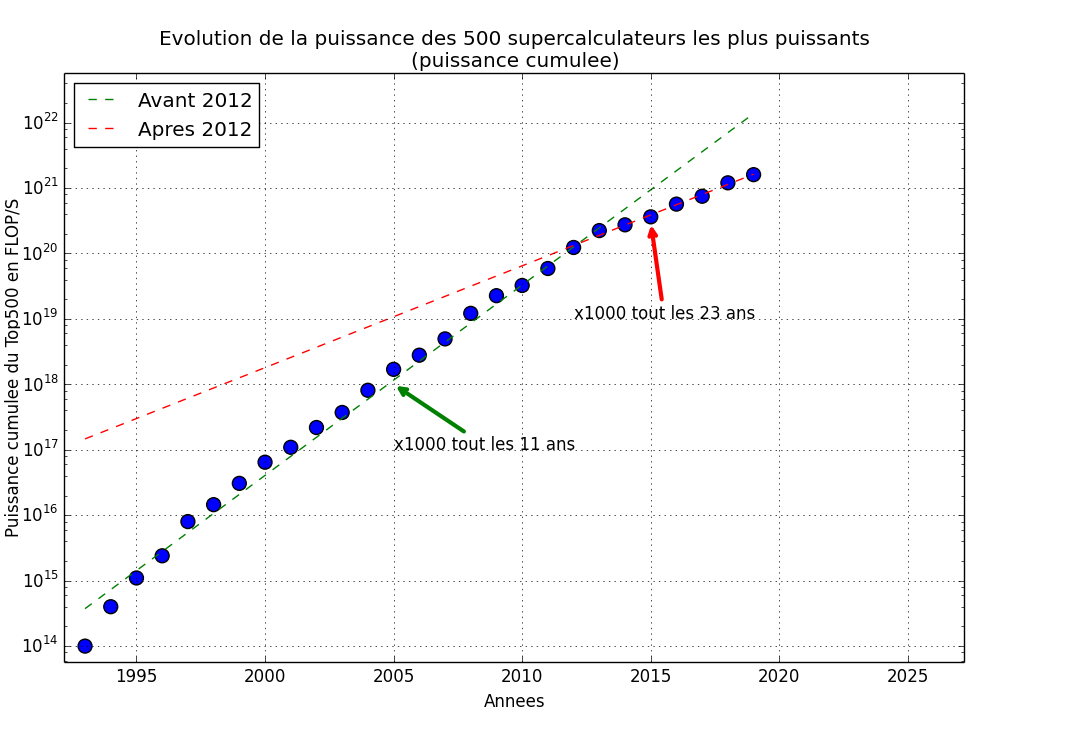
\includegraphics[width=14cm]{images/top500_evolution.png}
            \caption{\label{fig:top500_evolution_intro} Évolution de la performance cumulée des 500 supercalculateurs les plus puissants au monde, mesurée en FLOPS à l'aide du benchmark HPL (\textbf{todo accronyme}).}
        \end{figure}
        
        Nous remarquons sur la \autoref{fig:top500_evolution_intro} que la performance des supercalculateurs a évolué d'un facteur 1000 tous les 11 ans pendant près de 20 ans. Durant cette période, les processeurs ont pu profiter de nombreuses évolutions technologiques : augmentation du nombre de transistors et de la fréquence des processeurs, augmentation du nombre de coeurs ou encore l'implémentation d'une hiérarchie mémoire accélérant les accès aux données.
        Pour atteindre une puissance d'un exaflops, nous pouvons ainsi nous demander s'il ne suffirait simplement d'attendre les prochaines générations de processeurs et d'augmenter le nombre de serveurs formant un supercalculateur. Malheureusement, nous constatons à partir de 2012 un ralentissement de l'évolution des performances des supercalculateurs. Il faudra maintenant attendre 23 ans pour voir leur performance évoluer du même facteur 1000.
        Ce ralentissement est dû à un ensemble de contrainte qu'il n'est plus possible d'éviter, dont les deux principales sont la fin de la validité de loi de Moore, qui prévoyait l'augmentation du nombre de transistors chaque année, et la fin de la loi de Dennard, qui assurait l'augmentation les fréquences de chaque nouvelle génération de processeur.  De plus, les systèmes mémoires et les capacités de traitement des processeurs ont évolué de façon inégale. Lorsque la performance calculatoire augmentait de 50\% chaque année, le débit mémoire n'augmentait que de 23\%. Ce déséquilibre entre ces deux parties fondamentales de l'architecture Von Neumann a donné naissance au mur de la mémoire. À cause de cette inégalité d'évolution, les supercalculateurs modernes ne parviennent à extraire qu'une fraction des performances théoriques des architectures. Celle-ci  est parfois inférieure à 10\% \textbf{todo citer [Can+10]}.
        
        En plus des freins présentés ci-dessus, de nombreux défis supplémentaires doivent être relevés afin de poursuivre le rythme d'évolution des performances des supercalculateurs. Plusieurs études \cite{Sutter2005b, bergman2008exascale, Lucas2014, HPE2016} prédisent depuis plusieurs années les principales difficultés rencontrées pour développer une plateforme exascale : l'efficacité énergétique, les technologies d'interconnexion et mémoires, la gestion des données, la résistance aux erreurs… 
        Le principal défi est celui de l'énergie. Avec les technologies actuelles, un supercalculateur exascale consommerait plusieurs centaines de mégawatts, équivalent à la consommation électrique d'une ville comme Antibes (75 875 habitants). Pour des raisons de coût et de faisabilité, l'objectif de l'industrie HPC est de construire une plateforme exascale consommant entre 20 et 30 MW. Le challenge est donc de construire une plateforme sept fois plus puissante que le supercalculateur le plus puissant actuel, tout en étant trois fois plus efficace énergétiquement. Le déplacement des données à l'intérieur (entre la mémoire et le processeur) et à l'extérieur (entre deux serveurs) sont les principales opérations consommatrices d'énergie. Cette consommation peut être en partie expliquée par la complexité des microarchitectures, mais aussi par les technologies d'interconnexion utilisées. Cette complexité due aux nombreuses améliorations qu'ont connues les processeurs (hiérarchies mémoire, pipeline, d'unité de préchargement mémoire) est aussi à l'origine de la difficulté des applications à extraire plus d'une fraction des performances théoriques disponibles.
        

    \subsection{Les opportunités}


        L'incapacité des technologies actuelles à réaliser efficacement des calculs et l'explosion du nombre de données à traiter nécessite de repenser les matériels utilisés et l'architecture des systèmes informatiques. Heureusement de nouvelles technologies sont développées et peuvent permettre à l'industrie d'implémenter cette vision du calcul extrême.
        La première opportunité vient du développement de nouvelles technologies mémoires permettant de combler la différence d'évolution de performance constatée entre les processeurs et les mémoires. La faiblesse des débits mémoires et la consommation électrique du système mémoire obligent les architectures à évoluer drastiquement. La première solution est de rapprocher ces espaces mémoire des zones de calculs en plaçant la mémoire sur les puces de calculs (On Package Memory) ou en réalisant les calculs directement en mémoire (In Memory Computing).  La seconde solution est de développer de nouvelles technologies mémoires afin de combler le trou séparant les caractéristiques des mémoires DRAM et des disques de stockage flash. Pour cela des technologies NVRAM (non-volatile RAM) sont développées en s'appuyant notamment sur de nouvelles technologies mémoires SCM (storage class memory).
        Afin d'améliorer le débit des bus mémoire et d'interconnexion, des technologies photoniques sont actuellement développées. La principale qualité de ces technologies est d'être indépendant de la distance et de permettre d'atteindre des débits élevés. Bien que la génération d'un signal optique ou électronique nécessite la même énergie, celle-ci n'évolue que faiblement avec la distance de communication. Le coût énergétique d'un accès mémoire local est alors proche de celui d'un accès distant. 
        Ces nouvelles technologies, associées aux méthodes de co-design, qui associent les utilisateurs et les fabricants, vont permettre de développer de nouvelles architectures ultra-optimisées pour certains algorithmes.  L'utilisation d'architectures hétérogènes dans une même plateforme a été démocratisée par l'utilisation massive des GPU et doit être poursuivie avec de nouvelles architectures très différentes de celles actuellement utilisées : les accélérateurs produits par Google (TPU), NEC (SX-Aurora), ou encore Pezy (PEZY-SC2). 
        Afin de faciliter l'intégration de ces nouvelles technologies (mémoires, processeurs) provenant de différents constructeurs, de nouveaux protocoles doivent être développés. Un tel protocole est en cour de développement et propose un protocole de communication très simplifié utilisant une sémantique mémoire \verb=load/store=. Nommé Gen-Z, ce protocole est développé par 70 des plus grandes sociétés des technologies de l'information (IT). Il permettra d'adresser un espace mémoire mille fois plus grand que notre espace numérique actuel et interconnecter 16 millions d'objets sur une même fabric. Les premières versions d'architecture Gen-Z permettront d'atteindre des débits mémoires de plusieurs téraoctets par seconde contre quelques centaines de gigaoctets actuellement.

\section{Travail de thèse}

    
    Pour subvenir au besoin de puissance grandissant et ne pouvant compter sur les anciens leviers à sa disposition, l'industrie doit utiliser de nouvelles technologies émergentes et revoir la conception des plateformes de calculs. Ces ruptures technologiques sont telles, qu'elles permettront de faire des sauts de performance de plusieurs facteurs (10, 100 voir 1000).

    
    \subsection{Problématique}
    
        Grâce à Gen-Z et aux nouvelles technologies présentées précédemment, de nombreuses architectures vont être développées et seront très différentes de celles que nous utilisons actuellement (processeurs x86, GPU). Ces processeurs seront alors très efficaces pour l'exécution de certains types d'opérations et d'algorithmes. Afin de répondre aux besoins de performances supplémentaires et relever le défi de l'efficacité énergétique, il est nécessaire d'utiliser les architectures les plus adaptées pour l'exécution d'une application. Pour ce faire, trois tâches principales doivent être réalisées :
        \begin{enumerate}
            \item La première tâche est de caractériser l'ensemble de ces architectures pour trouver leurs forces et leurs faiblesses: débit et latence mémoire, capacité calculatoire, performance du système mémoire pour certains motifs d'accès. Ces nouvelles architectures pouvant être très différentes de celles que nous utilisons actuellement, il est indispensable de disposer d'un ensemble d'outils permettant de les caractériser pour différents types d'algorithmes.
        
            \item La deuxième tâche consiste à modéliser les performances d'une application pour en connaître ses besoins (débit et/ou latence mémoire, calcul vectoriel, système d'interconnexion, stockage…). Les gains de performance ne viendront pas seulement de l'utilisation d'accélérateurs puissants, mais de leur diversité et de la capacité des programmeurs à bien les utiliser. Pour une même application, plusieurs zones de code prenant une part importante dans son exécution peuvent avoir des besoins différents. Il est ainsi nécessaire de pouvoir identifier ces zones et de les modéliser indépendamment. 
        
            \item La troisième tâche est de sélectionner les architectures adéquates pour une application et adapter le code pour permettre son exécution. Il est ensuite nécessaire de pouvoir mesurer les performances de l'application et d'appliquer les optimisations adaptées pour obtenir une part significative de la performance théorique.
        \end{enumerate}
    
    \subsection{Travaux existants}
    
        Afin de répondre aux tâches présentées ci-dessus, les programmeurs doivent alors avoir à leur disposition un ensemble d'outils permettant de caractériser le comportement des architectures et d'étudier la performance de leurs applications lors de l'exécution.
        
        
        \subsubsection{Caractérisation des architectures}
            
            Afin de caractériser les architectures et de mesurer les performances atteignables par la microarchitecture, il est courant d'utiliser des benchmarks. En informatique, un benchmark est un code, ou un ensemble de codes, permettant de mesurer la performance d'une solution et d'en vérifier ses fonctionnalités. Dans ce travail de thèse, nous nous intéressons à la caractérisation de deux composants fondamentaux des processeurs utilisés en HPC : la hiérarchie mémoire et les unités de calcul vectorielles. 
            
            \paragraph{Caractérisation du système mémoire} 
            
                Le système mémoire étant le goulot d'étranglement principal des performances des applications, de nombreux travaux ont été menés pour aider à sa caractérisation. Le plus utilisé d'entre eux est le benchmark STREAM \cite{McCalpin1995}. Ce code utilise 4 noyaux de calculs différents pour mesurer le débit mémoire atteignable par une architecture. Pour cela, un tableau de nombres aléatoires stocké en mémoire est accédé par des instructions de lecture/écriture pour réaliser 4 opérations : copy, scale, add, triad. La simplicité de ces codes permet souvent d'atteindre les débits maximaux du bus mémoire et fait de STREAM un benchmark de référence. Un autre benchmark largement utilisé dans l'industrie est celui de Lmbench \cite{Staelin2004}. Lmbench est une suite de microbenchmarks utilisée pour mesurer la latence et le débit atteignable par un cœur pour différentes opérations : accès mémoire, ouverture de fichier, création de pipe. Il permet aussi de trouver certaines caractéristiques de la microarchitecture comme la taille d'une ligne de cache ou de celle de la TLB \textbf{todo TLB}.
                
                De nombreuses applications utilisent des accès mémoires réalisant des sauts d'adresses (stride) de taille constante. Par exemple, le parcours d'un tableau d'objet pour accéder à un certain champ ou le parcours d'une matrice (en ligne ou en colonne). Pour accélérer ces accès, l'unité de préchargement mémoire peut anticiper les prochaines adresses accédées en comprenant le motif d'accès utilisé et commencer leur chargement avant qu'elles ne soient accédées. Pour des applications utilisant ce type d'accès par saut, il est primordial que ce composant fonctionne correctement pour réduire au maximum le manque d'une donnée dans le cache lors de son accès.
                Au moment de la réalisation de ce travail de thèse, il n'existe à notre connaissance aucun benchmark permettant de caractériser l'architecture pour ce type d'accès. Le benchmark s'approchant le plus de cet objectif est celui de Saavedra  \cite{Saavedra1995}.  Il utilise une taille de saut fixée au début de l'exécution pour accéder à un jeu de données. La taille de ce dernier doit être un multiple d'une puissance de 2 et ne permet pas de dépasser la taille du dernier niveau de cache. Le problème d'une telle approche est de vouloir mesurer tous les niveaux de la hiérarchie simultanément. Les mesures peuvent alors être influencées par différents paramètres de différents niveaux de caches.
        
            \paragraph{Caractérisation des unités de calculs vectorielles}
            
                La majorité des applications utilisées en HPC exécutent des \gls{FLOP}. Ces instructions sont exécutées par un matériel spécialisé nommé \gls{ALU}. La capacité des ALU à exécuter plusieurs instructions vectorielles par cycle est alors primordiale pour la bonne performance des applications. La littérature dénombre plusieurs benchmark couramment utilisés pour mesurer la performance de calcul des processeurs. Le benchmark HPL  \cite{Dongarra2003} a été développé pour caractériser la microarchitecture d'un processeur lors de la résolution de problèmes algébriques. Ce code permet aujourd'hui de mesurer et classer les supercalculateurs dans le classement du Top500. Le benchmark HPL n'étant pas représentatif d'applications réelles, un ensemble de codes a été rassemblé pour améliorer la caractérisation des supercalculateurs. Nommé HPCG \cite{Dongarra2013}, cet ensemble de codes permet de couvrir plusieurs motifs de communication et de calculs. Les versions récentes du Top500 publient pour certains supercalculateurs la performance obtenue sur le benchmark HPCG. Nous pouvons aussi citer le benchmark HPCC \cite{Luszczek2006} qui est une suite de 6 benchmarks contenant notamment HPL et STREAM. Un seul exécutable est généré pour l'ensemble de la suite permettant d'éviter l'utilisation de certaines optimisations pour un code particulier (pages larges, réglage BIOS…). 

                Nous constatons le manque d'un outil permettant de valider précisément les performances des unités de calculs. Un tel outil permettrait en effet d'étudier le comportement précis des ALU : le nombre d'instructions par cycle pour différentes opérations vectorielles, la possibilité de combiner des instructions différentes, la sensibilité aux chaînes de dépendances.
                
                
        \subsubsection{Suivi de performance des applications}
        
            Le deuxième aspect de nos recherches concerne le suivi de performances des applications. L'objectif de celui-ci est de récolter des informations concernant l'application ou le système. Ces informations peuvent être obtenues en instrumentant le code (manuellement ou grâce au compilateur) ou en récupérant certaines informations de l'architecture. Pour cela, les processeurs possèdent des registres (compteurs) qui permettent de compter des événements (matériels ou logiciels) avec un faible impact sur l'application exécutée. Chaque famille de processeurs possède un jeu différent de compteurs matériels pouvant avoir des noms différents, rendant leur programmation difficile. Afin de faciliter leur programmation, des interfaces comme \verb=PAPI= \cite{Browne2000} et \verb=Perf Events= \cite{Weaver2013} ont été développées. Celles-ci permettent de développer des outils sans se préoccuper de l'implémentation matérielle des compteurs facilitant ainsi la portabilité des outils. Nous pouvons notamment citer les outils d'Intel (\verb=VTune=), de Linux (\verb=perf=) ou encore ceux développés au Barcelona Supercomputing Center (\verb=Extrae= \cite{Rodriguez}, \verb=Paraver= \cite{Pillet1995} et \verb=Dymemas= \cite{Labarta1997}).
            
            Afin de répondre aux différentes tâches de la problématique traitée dans ce travail de thèse, deux outils principaux sont nécessaires. 
            Le premier doit permettre de suivre l'activité du bus mémoire. Ce bus est une ressource critique des architectures modernes, rendant sa bonne utilisation indispensable. Il est donc nécessaire de posséder un outil permettant de suivre l'état du trafic sur ce bus. Pour cela, des outils existent, mais sont soit propriétaires, soit trop complexes pour être facilement installés sur des architectures novatrices. 
            Un second outil doit être capable d'extraire les zones de codes les plus intéressantes à porter sur ces nouvelles architectures. Les supercalculateurs seront hétérogènes et utiliseront plusieurs accélérateurs différents adaptés à certaines fonctions. Une même application pourra alors faire appel à plusieurs d'entre eux. Il est donc nécessaire de posséder un outil permettant de caractériser les différentes fonctions d'une même application en extrayant ces zones de codes et en les caractérisant.  Ce même outil pourrait alors aussi être utilisé pour comprendre les performances de l'application et appliquer les optimisations adéquates. 

\section{Contributions et plan du manuscrit}
    
    L'industrie va faire face à une multitude de révolutions technologiques, et les utilisateurs de supercalculateur doivent se préparer à ces changements profonds pour pouvoir les exploiter au maximum. Contrairement aux évolutions précédentes où il suffisait d'installer un nouveau processeur ou d'ajouter des barrettes mémoires, il faut repenser entièrement notre façon d'appréhender les architectures des supercalculateurs et adapter les algorithmes qui y seront exécutés. Cependant, en l'absence de méthode de caractérisation fine de la performance des codes, ces architectures innovantes sont potentiellement condamnées puisque peu d'experts savent les valoriser. En effet, la loi de Moore a permis d'assurer une évolution constante des processeurs, laissant le domaine de l'analyse et l'optimisation des codes en second plan. Ainsi, nous avons constaté à travers de nombreuses rencontres avec les utilisateurs, mais aussi par les expériences internes à HPE, le manque d'outils et de connaissances nécessaires à la réalisation de ce travail.
    
    \subsection{Contributions}
        
        Afin de pouvoir profiter de ces nouvelles technologies, nous proposons dans ce travail une méthodologie en 5 étapes permettant de modéliser les performances d'une application, de les projeter sur de nouvelles architectures et d'en extraire la performance maximale. Pour chaque étape, nous avons développé et sélectionné des outils permettant de répondre aux challenges présentés et qui respectent certains critères :
        \begin{itemize}
            \item Les sources de l'outil doivent être disponibles pour permettre de les adapter à des architectures différentes et pour développer une communauté d'utilisateurs autour de ces sujets,
            \item Les outils doivent être simples, ne cherchant pas à répondre à une multitude de questions qui rendent difficile leur portabilité, mais aussi les conclusions pouvant être tirées des résultats obtenus,
            \item Les outils doivent permettre d'analyser des applications HPC dont l'exécution peut durer plusieurs heures. Il faut aussi réduire au maximum la nécessité de posséder des droits spéciaux (root) pour les utiliser, ce dernier étant rarement disponible pour les utilisateurs de supercalculateurs.
        \end{itemize}
        
        Les outils n'ont pas vocation d'automatiser entièrement les tâches du programmeur. La puissance de ces outils vient de leur utilisation complémentaire. Nous espérons qu'en réduisant la complexité de l'outillage, l'adoption des outils auprès des programmeurs sera plus grande. Nous avons développé un outil lorsqu'aucun programme existant ne pouvait être utilisé pour la réalisation d'une étape de la méthodologie, ou qu'il ne respectait pas les critères énoncés ci-dessus. Les principales contributions de cette thèse sont :
        \begin{enumerate}

            \item \textbf{Un benchmark mémoire} – \verb=DML_MEM= : ce benchmark permet de mesurer le débit mémoire en réalisant des accès dans un tableau avec des motifs de sauts (strides). La taille du tableau et des sauts peut varier et permet de caractériser les différents niveaux de la hiérarchie mémoire. Cet outil est utile pour caractériser une nouvelle architecture, mais peut aussi être utilisé lors du design d'un nouveau processeur pour vérifier le bon fonctionnement du préchargement mémoire.
            
            \item \textbf{Un benchmark d'unité arithmétique et logique (ALU)} – \verb|Kernel Generator| : ce générateur permet de caractériser finement les performances des unités arithmétiques et logiques (ALU). Pour cela, il génère un benchmark assembleur en utilisant des instructions vectorielles de taille différentes (SSE, AVX2, AVX-512). L'utilisateur peut alors choisir le type d'opération à exécuter (addition, multiplication, FMA) et la précision (simple, double). La partie du benchmark mesurée ne contient que des instructions de calculs et permet de mesurer très précisément la performance atteignable pas le processeur (souvent proche ou égale à la performance théorique).
                        
            \item \textbf{Un outil de suivi d'activité du bus mémoire} -  \verb=YAMB= : cet outil est basé sur l'interface perf et permet de mesurer le trafic mémoire sur le bus en discernant les lectures et les écritures. YAMB établit le profil de chaque contrôleur mémoire en mesurant le nombre de transactions (lecture et écriture) ainsi que le nombre d'accès manqués (miss) dans le dernier niveau de cache (LLC). Pour corréler l'activité du bus avec les parties du code qui en sont responsables, le graphique peut facilement être annoté en utilisant une API C/C++/Fortran, appelée directement depuis le code source.
            
            \item \textbf{Un outil extraction des \glspl{kernel}} – \verb=Oprofile++=: cet outil permet de désassembler le code d'une application, d'extraire les boucles critiques d'en mesurer la performance. Oprofile++ est basé sur les outils Oprofile et Objdump. Il permet dans un premier temps de relier le profile aux instructions assembleurs exécutées. Ensuite, il s'occupe d'extraire les boucles critiques et de mesurer le nombre d'instructions exécuté chaque cycle (IPC). Il est ensuite possible de quantifier des opportunités d'amélioration, mais aussi de prédire la performance en fonction d'une amélioration du matériel ou du logiciel.
            
            \item \textbf{Une méthodologie pour le portage et l'optimisation} : Afin d'utiliser de façon efficace les outils sélectionnés et développés, nous avons décrit une méthodologie en 5 étapes. Celle-ci permet de sélectionner la meilleure architecture pour une application donnée et d'en extraire le maximum de performance.
        
        \end{enumerate}
        
    \subsection{Plan du manuscrit}
    
        Cette thèse propose une étude étendue du domaine du HPC pour comprendre et contribuer à l'élaboration des prochaines générations de plateformes de calculs. Pour cela, le manuscrit suit la structure suivante :
        
        \begin{itemize}
        
            \item Le \autoref{chap:hpc} introduit le domaine du calcul haute performance en étudiant ses origines et en présentant leur architecture actuelle et les moyens employés pour les programmer. Nous discutons ensuite de leur performance en étudiant l'évolution du classement du Top500 et nous expliquons notamment les principaux freins qui empêchent de construire des plateformes toujours plus puissantes avec les méthodes actuelles. Afin d'y parvenir, nous présentons les principales opportunités technologiques actuellement développées qui vont nous permettre de repenser l'architecture des plateformes. La fin de ce chapitre s'intéresse plus précisément à la caractérisation des microarchitectures et à l'analyse de performance d'applications.
        
            \item Le \autoref{chap:dev} présente les principaux outils développés durant ces travaux de thèse. Nous discutons des motivations et des critères de développement qui nous ont conduits à développer deux benchmarks et deux outils d'analyse de performance.
        
            \item Le \autoref{chap:methodo} présente en détail la méthodologie élaborée et utilisée pour caractériser et choisir une architecture pour une application donnée. Nous utilisons l'analyse du benchmark STREAM et d'un processeur Intel Skylake pour illustrer chacune des 5 étapes.
        
            \item Afin de permettre la réalisation des différents codes développés, l'étude approfondie des différentes évolutions technologiques des processeurs et des techniques de suivi de performances sont présentées dans deux annexes de ce manuscrit:
            \begin{itemize}
                \item L'\aref{annexe:CHAPITRE_ARCHITECTURE} couvre l'origine et l'évolution de la microarchitecture des processeurs. Nous présentons les fonctionnalités clés des processeurs modernes qu'il est nécessaire de connaître pour comprendre la performance des applications: pipeline, instructions vectorielles, etc. Nous étudions plus précisément la hiérarchie mémoire qui est la ressource critique de nombreuses applications. 
                
                \item L'\aref{annexe:hardware_counter} présente les compteurs matériels. Ces registres spéciaux du processeur permettent de suivre l'exécution d'une application en mesurant le nombre d'évènements logiciels et matériels. La programmation des compteurs est très difficile et nécessite le recours à des codes bas niveaux. Plusieurs méthodes peuvent alors être employées et demandent une bonne expérience pour être mise en oeuvre.
            \end{itemize}
            Nous faisons référence à ces deux annexes lorsque les concepts qui y sont étudiés sont utilisés dans le manuscrit.
        
        \end{itemize}
    \fi 


    %% EDL HPC %%    
    \iflong
        \chapter{Calcul Haute Performance}\label{chap:hpc}
\minitoc


Ce chapitre présente le domaine du HPC et réalise un état de l'art du domaine afin de motiver la nécessité de repenser l'architecture des supercalculateurs mais aussi d'utiliser de nouvelles technologies. Pour comprendre quels challenges doivent être relevés, nous étudions le classement du Top500 et synthétisons les principaux freins au développement des performances des plateformes. Nous présentons ensuite les principales technologies qui devront être utilisées pour parvenir à développer de telles architectures malgré les contraintes énergétiques. Le chapitre se termine par l'étude des outils permettant la caractérisation et le suivi de performance des applications.

\section{Introduction au Calcul Haute Performance (HPC)}\label{sec:hpc_intro}


\subsection{Le calcul scientifique et la simulation numérique}
%%%%%%%%%%%%%%%%%%%%%%%%%%%%%%%%%%%%%%%%%%%%%%%%%%%%%%%%%%%%%%

    À l'origine, les scientifiques observaient la nature et émettaient des théories pour expliquer leurs observations (voir \autoref{fig:edl_simu_new}). En se basant sur ces théories, ils réalisaient des expériences physiques pour les valider ou non. Ils faisaient alors de nouvelles expériences pour affiner leur théorie. Les simulations numériques sont alors apparues comme des alternatives aux expériences physiques qui étaient souvent longues et onéreuses (voir \autoref{fig:edl_simu_new}). Des scientifiques comme Pythagore réalisaient ces simulations en faisant des calculs manuels ou en s'aidant de tables précalculées. Du fait de la limitation de leur capacité de calcul et de temps disponible, c'est avec l'apparition de l'informatique que les simulations sont devenues réellement exploitables.
    
    
    \begin{figure}[b!]
        \centering
        \begin{subfigure}[t]{0.48\textwidth}
            \centering
            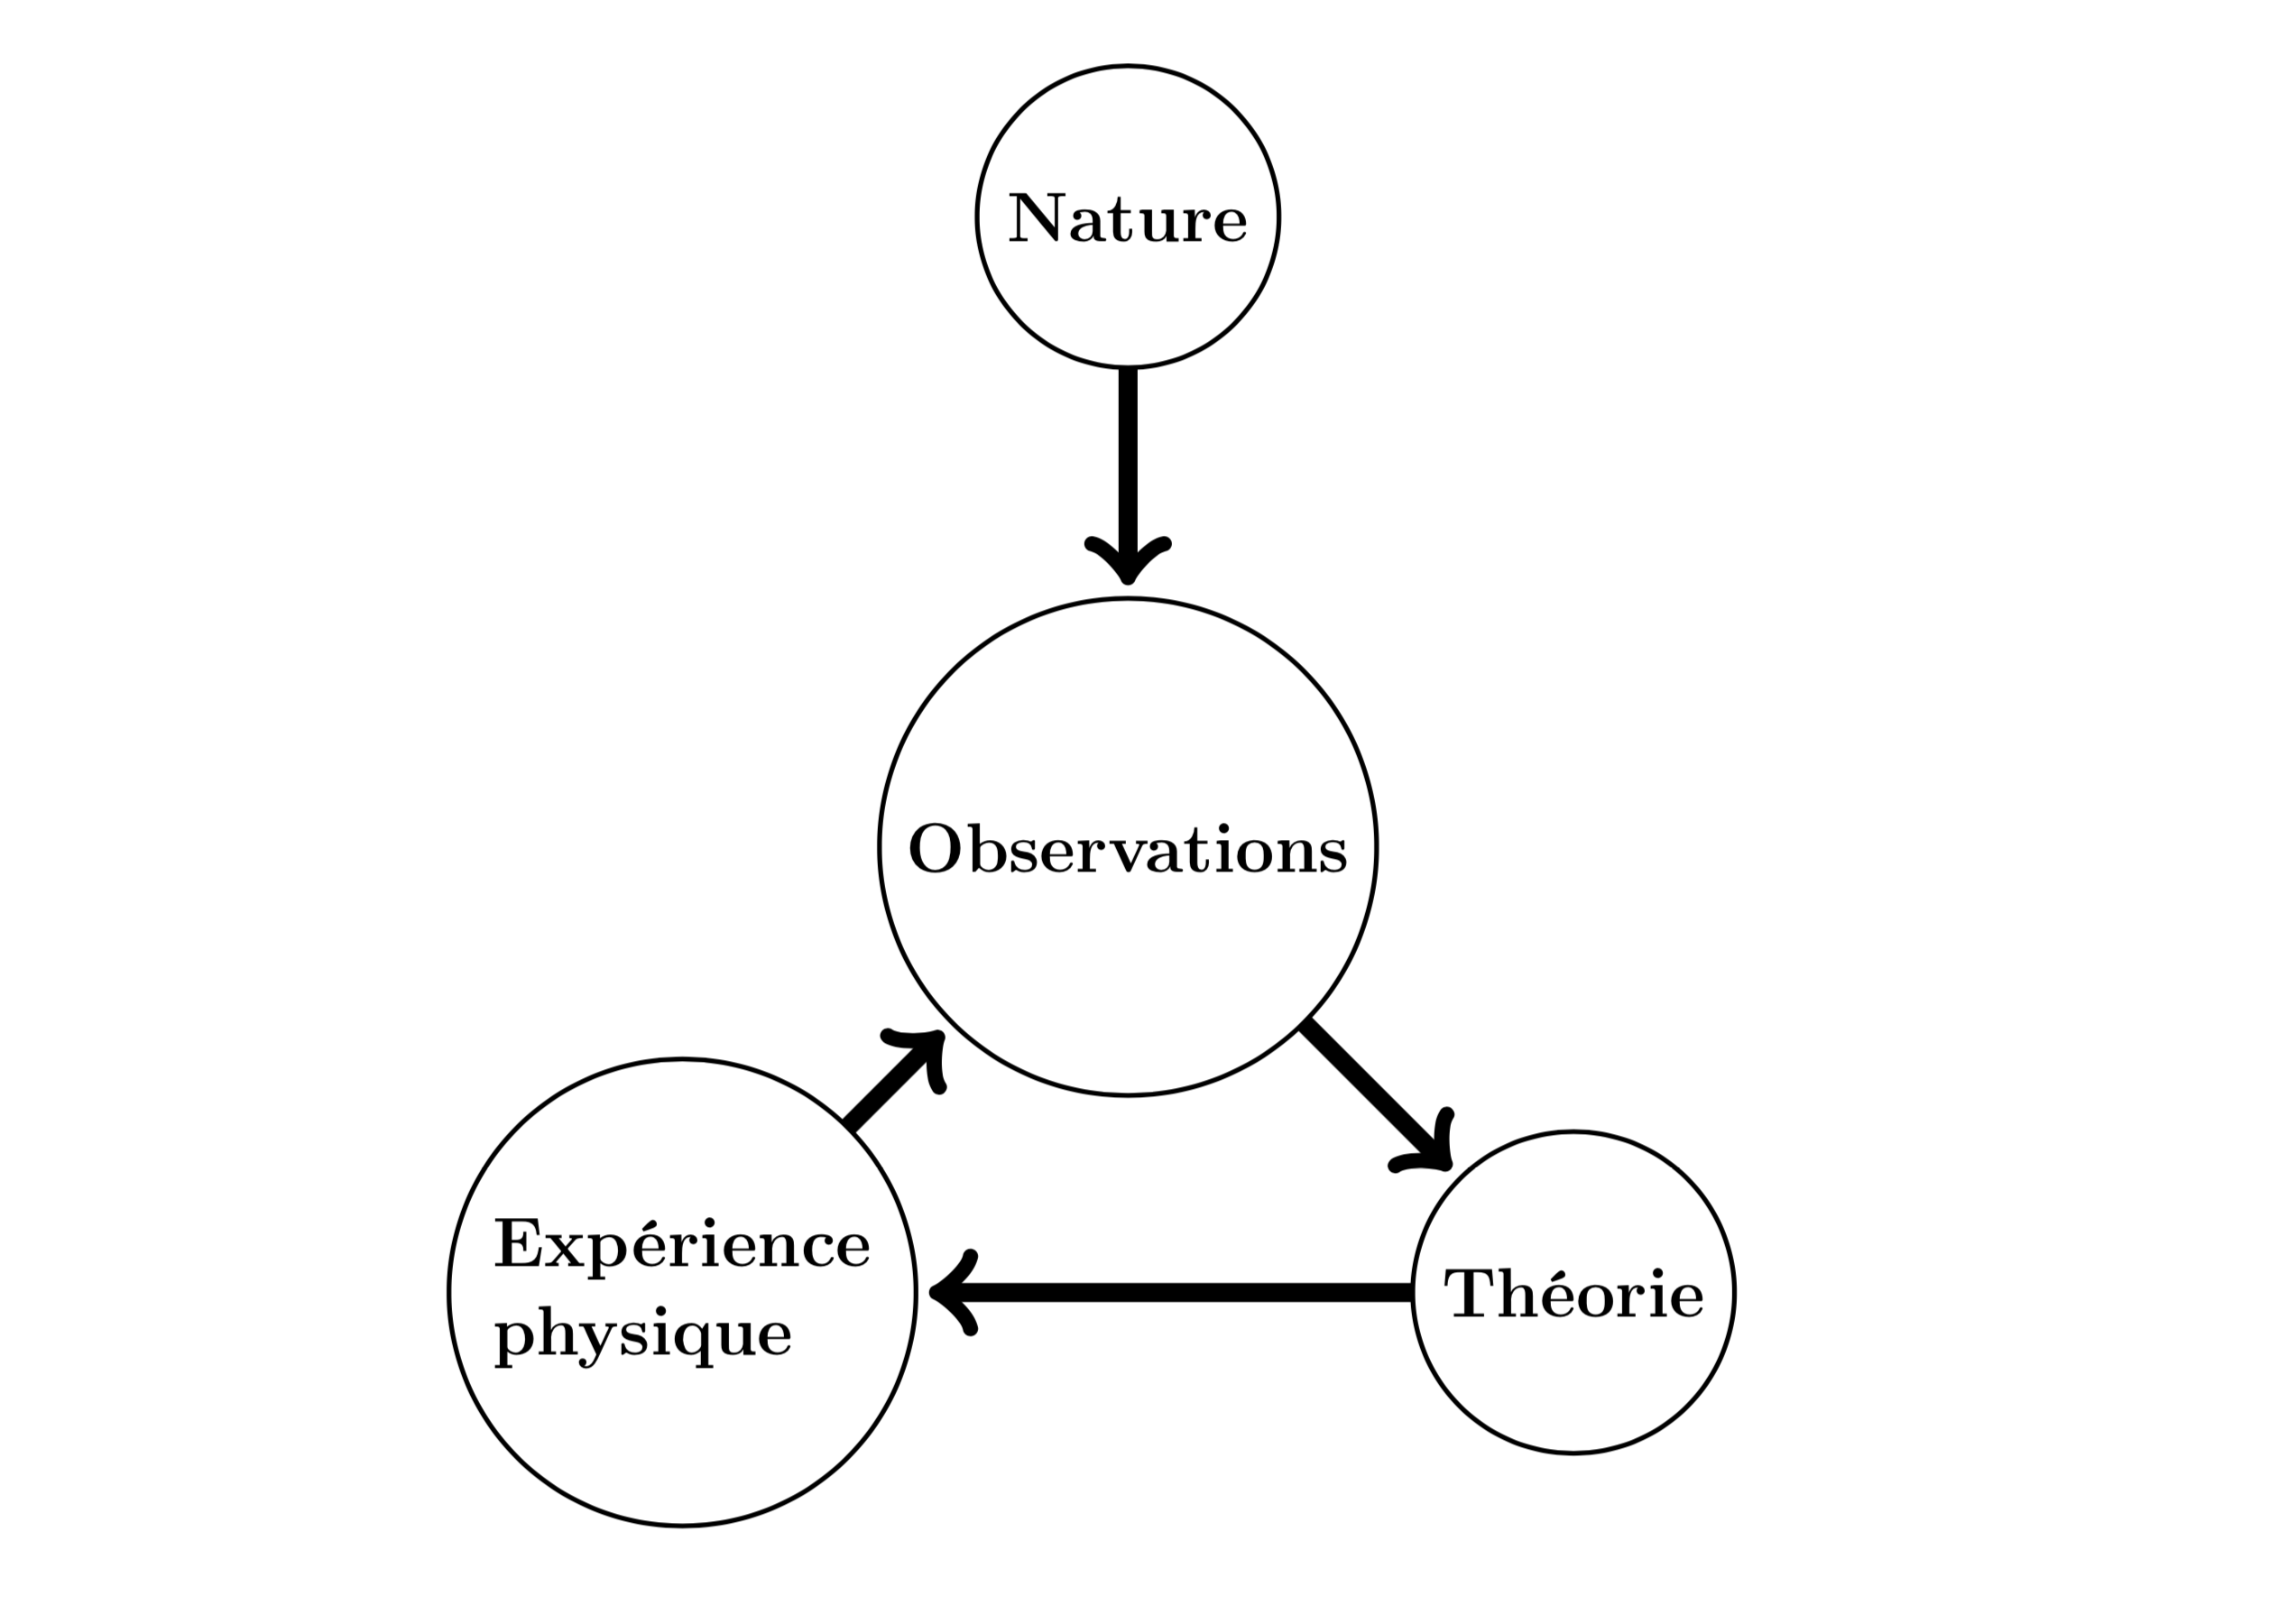
\includegraphics[width=\linewidth]{images/edl_simu_old.png}
            \caption{\label{fig:edl_simu_old}Les expériences physiques permettent de valider les théories.}
        \end{subfigure}\hfill
        \begin{subfigure}[t]{0.48\textwidth}
            \centering
            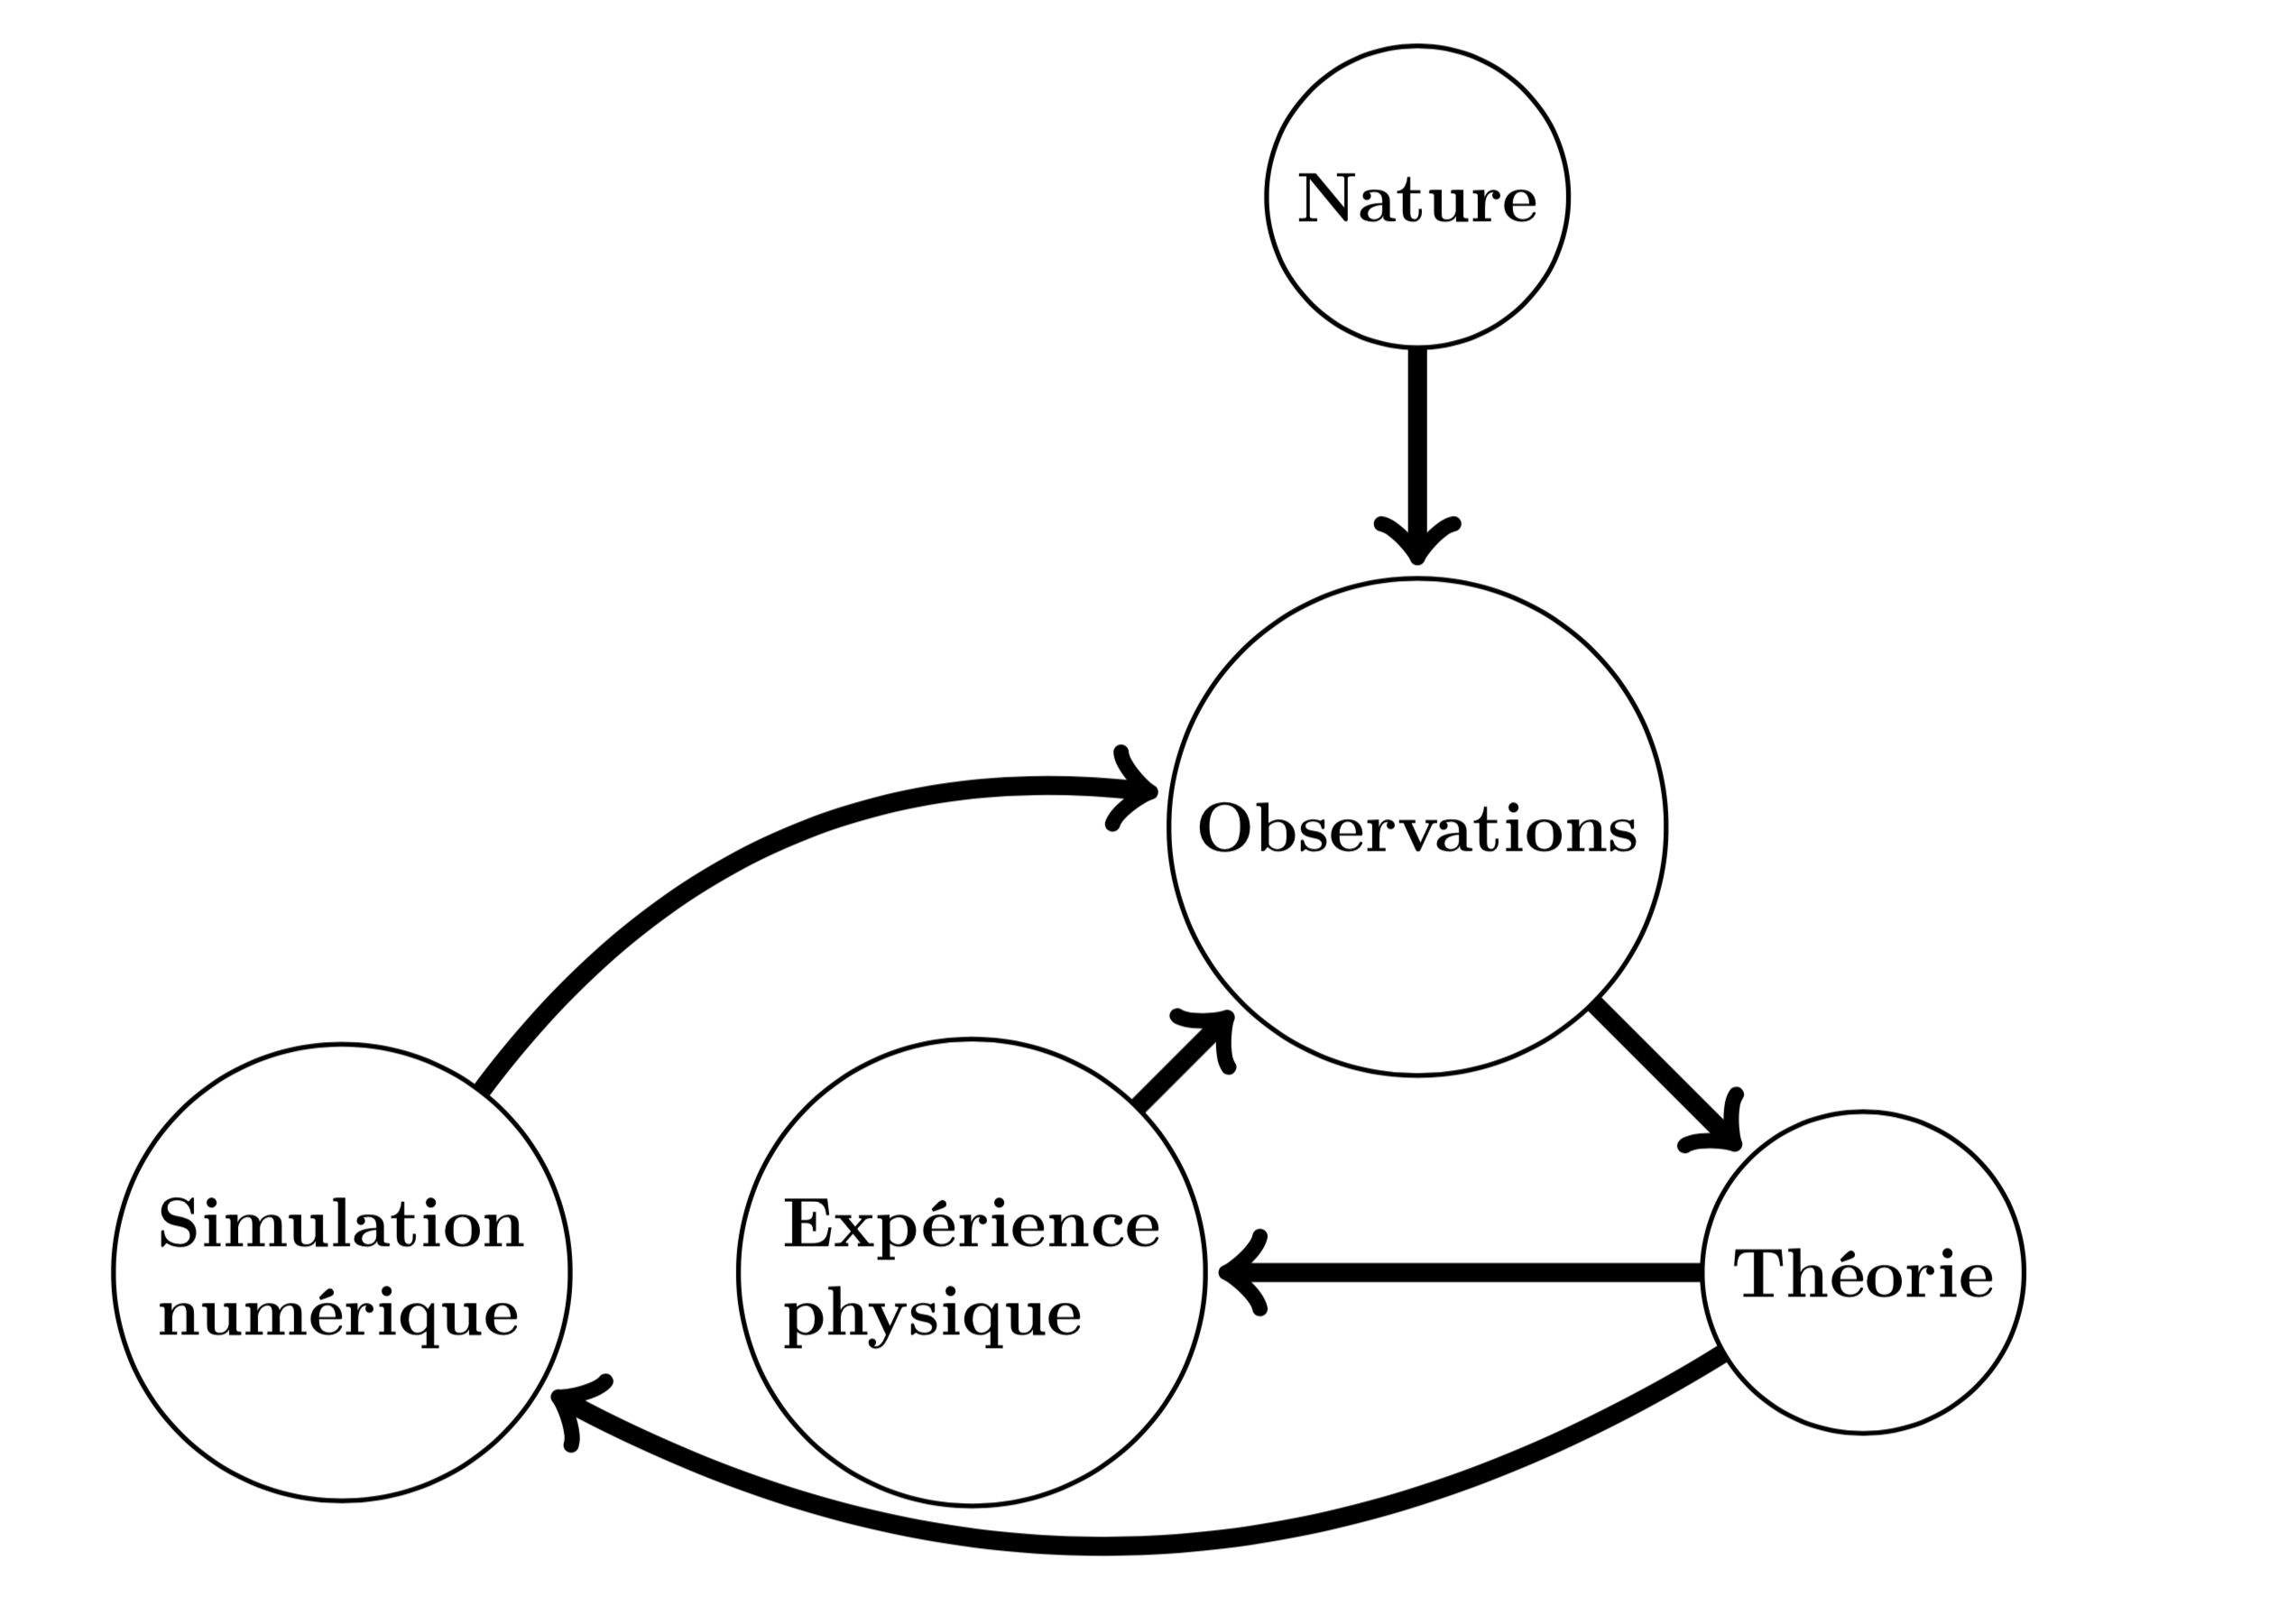
\includegraphics[width=\linewidth]{images/edl_simu_new.png}
            \caption{\label{fig:edl_simu_new}La simulation numérique peut être une alternative aux expériences physiques.}
        \end{subfigure}
        \caption{La simulation numérique a apporté une nouvelle façon d'expérimenter les théories.}
        \label{fig:tikz_simulation}
    \end{figure}
    

      
    %TikZ picture
%\begin{figure}
%\begin{center}
%\begin{minipage}[]{.5\textwidth}
%\begin{tikzpicture}[->,shorten >=1pt,auto,node distance=3.8cm,   scale=0.49, every %node/.style={transform shape}]
%\tikzstyle{every state}=[fill=none,draw=black,text=black,  , font=\bf]
%\tikzstyle{edge_style} = [draw=black, line width=2, ultra thick]
%\tikzstyle{node_style} = [circle,draw=blue,fill=blue!20!,font=\sffamily\Large\bfseries]
%\node[state]					    (A)                     {Nature};
%\node[state]        				(B) [below of=A]        {Observations};
%\node[state,]         		    (D) [below right of=B]  {Théorie};
%\node[state, align=left]         	(C) [below left of=B]   {Expérience\\ physique};
%\path
%(A) edge [edge_style]   node {} (B)
%(B) edge [edge_style]   node {} (D)
%(C) edge [edge_style]   node {} (B)
%(D) edge [edge_style]   node {} (C);
%\end{tikzpicture}
%\end{minipage}%
%\begin{minipage}[]{.5\textwidth}
%\begin{tikzpicture}[->,shorten >=1pt,auto,node distance=3.8cm,   scale=0.49, every %node/.style={transform shape}]
%\tikzstyle{every state}=[fill=none,draw=black,text=black,  , font=\bf]
%\tikzstyle{edge_style} = [draw=black, line width=2, ultra thick]
%\tikzstyle{node_style} = [circle,draw=blue,fill=blue!20!,font=\sffamily\Large\bfseries]
%\node[state]					(A)                    {Nature};
%\node[state]        					(B) [below of=A] {Observations};
%\node[state,]         					(D) [below right of=B] {Théorie};
%\node[state, align=left]         	(C) [below left of=B] {Expérience\\ physique};
%\node[state, align=left]        	(E) [left of=C]       {Simulation\\numérique};
%\path
%(A) edge [edge_style]            node {} (B)
%(B) edge [edge_style]     node {} (D)
%(C) edge [edge_style]           node {} (B)
%(D) edge [edge_style]             node {} (C)
%edge [edge_style, bend left]     node {} (E)
%(E) edge [edge_style, bend left]  node {} (B);
%\end{tikzpicture}
%\end{minipage}
%\end{center}
%\caption{La simulation numérique a apporté une nouvelle façon d'expérimenter les théories.} 
%\label{fig:tikz_simulation}
%\end{figure} 
     
    
     
    \subsubsection{Principe de la simulation numérique}
    %%%%%%%%%%%%%%%%%%%%%%%%%%%%%%%%%%%%%%%%%%%%%%%%
    
        La majorité des simulations numériques sont basées sur des équations dites \textit{gouvernantes} et qui sont des approximations des phénomènes étudiés. Ces équations ont besoin d'être discrétisées pour pouvoir être exécutées par un ordinateur. En mathématiques, la discrétisation est un procédé qui permet de passer d'un modèle à son équivalent discret. Ce procédé ne permet pas de décrire le phénomène réel, mais de l'approcher avec plus ou moins d'erreurs. Pour améliorer ces simulations, ces représentations doivent utiliser des maillages les plus fins possible (voir \autoref{pic_maillage}). Une autre approche utilise des modèles probabilistes pour représenter un comportement. Elle est adaptée pour des phénomènes où chaque élément peut subir différents événements. Pour chaque étape du calcul, le résultat évolue grâce à des tirages aléatoires (méthode de Monte-Carlo \cite{Kroese2014}). Pour améliorer la précision des simulations, il est donc nécessaire d'augmenter le nombre de tirages et donc le nombre de calculs à réaliser.
        Que ce soit pour affiner la taille des maillages ou augmenter le nombre de tirages, les simulations numériques nécessitent de grandes puissances de calculs. 
            
            \begin{figure}
            \center
            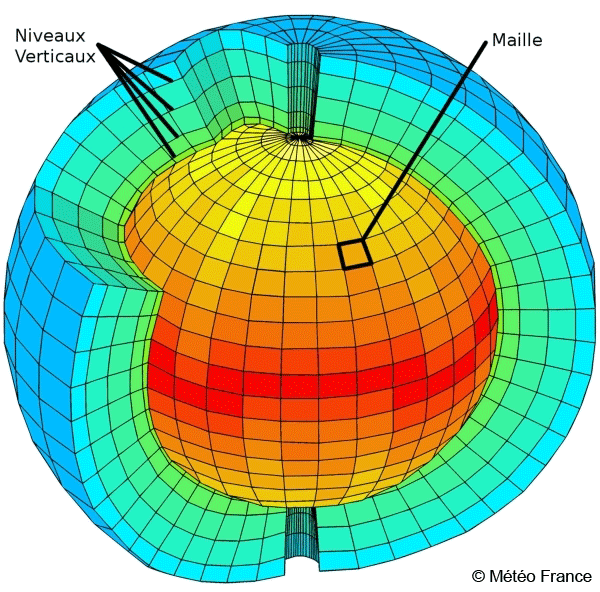
\includegraphics[width=5cm]{images/Chapitre1/maillage.png}
            \caption{\label{pic_maillage} Le maillage le plus fin exploité par Météo-France pour ses prévisions régionales restitue des mailles de 2,5 km de côté (source \url{www.irma-grenoble.com}).}
            \end{figure}

    
    \subsubsection{Quelques applications de simulations numériques}
    %%%%%%%%%%%%%%%%%%%%%%%%%%%%%%%%%%%%%%%%%%%%%%%%
        Lorsque l'on évoque la simulation numérique, on pense souvent aux domaines physiques (météorologie, mécanique, biologie), mais elle peut aussi être utilisée en sciences humaines (sociologie, analyse démographique) ou dans le domaine de la sécurité nationale. En effet, Alan Turing a développé les premiers ordinateurs lors de la fin de la Deuxième Guerre mondiale pour aider au décryptage des messages allemands. En 1936, il avait présenté les premiers concepts de programmes et donné naissance à l'aide d'une expérience de pensée à l'ancêtre des ordinateurs nommée machine de Turing. L'utilisation de simulations numériques a de nombreux avantages. En plus de profiter de la puissance de calculs des ordinateurs, elle permet de simuler des phénomènes dont les conditions ne sont pas reproductibles sur terre (physique théorique). Un autre avantage est de réduire drastiquement les coûts d'une expérience, par exemple pour la réalisation de crash automobile, où ce ne sont plus de réels modèles de voiture, mais bien des voitures virtuelles qui sont crashées sur des murs.
        
        Dans le domaine de la santé, l'étude de la structure des protéines est primordiale.  Ces molécules qui assurent les fonctions élémentaires d'une cellule interviennent dans la majorité des processus biologiques (régulation du métabolisme, défense immunitaire). Dans ce genre de simulation, le pas de temps est de l'ordre de la nanoseconde. Grâce à la simulation numérique, une meilleure compréhension de ces molécules permet la découverte de nouveaux médicaments ou antibiotiques. 
        Aussi, des modélisations peuvent être utilisées pour analyser la propagation d'un virus comme la grippe aviaire à l'échelle mondiale pour mieux protéger les populations\cite{CEA2007}. En février 2020, le gouvernement français indiquait travailler sur la modélisation de la propagation du COVID-19\footnote{\url{https://www.gouvernement.fr/info-coronavirus}} (coronavirus). Cette modélisation fait intervenir plusieurs paramètres comme le lieu et la période d'incubation du virus ou encore la fréquentation et les destinations des passagers des 4000 principaux aéroports mondiaux. En mars 2020, le supercalculateur le plus puissant au monde (Summit) était utilisé pour identifier 77 molécules potentiellement efficaces contre le COVID-19 \cite{Smith2020}.

        En astrophysique, la simulation numérique est aussi capitale du fait de la non-reproductibilité des expériences en laboratoire.  À l'opposé de l'exemple précédent sur les protéines, elle permet d'étudier des objets aussi grands que complexes comme le système solaire, les galaxies ou bien l'univers. La simulation permet alors de faire évoluer le système avec un pas de temps allant jusqu'au million d'années. Une équipe du CEA a pu reconstituer le passé de la galaxie Andromède en analysant les observations réalisées grâce au satellite infrarouge Spitzer\cite{Block2006}. Après avoir mis au point le modèle adéquat et après plusieurs heures de simulation, ils ont pu déterminer qu'elle avait été percutée par une galaxie voisine il y a plus de 210 millions d'années et que sa forme actuelle résultait de cet impact (voir\autoref{pic:cea_galaxy}).
    
        
        \begin{figure}
            \center
            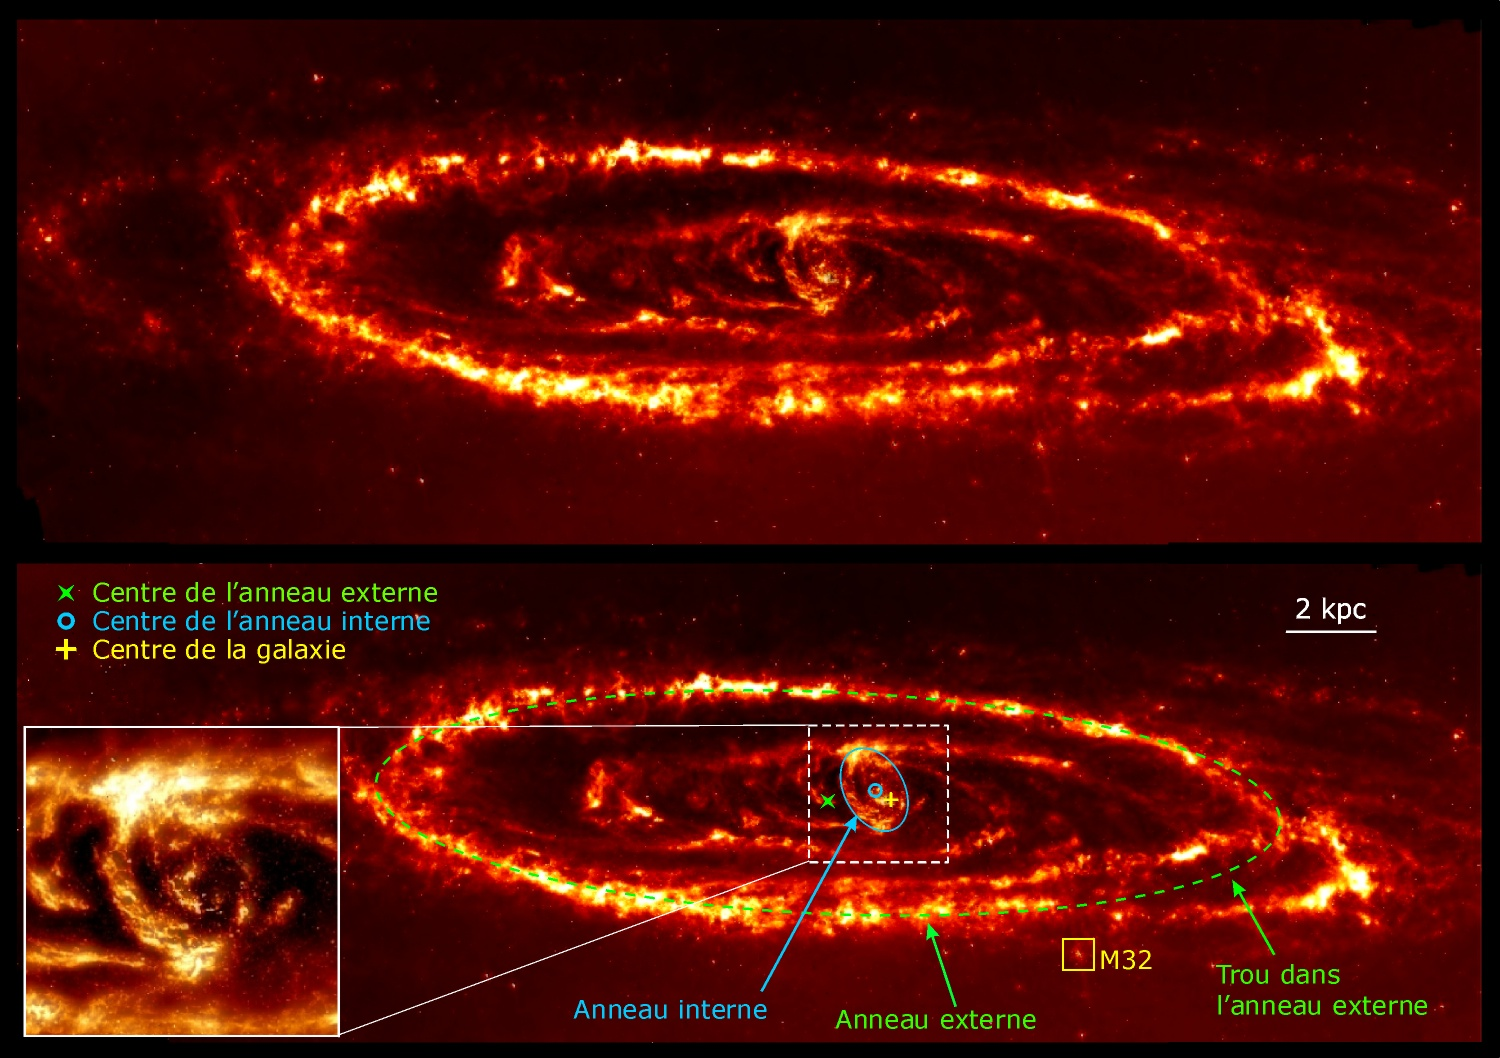
\includegraphics[width=12cm]{images/cea_galaxy.jpg}
            \caption{\label{pic:cea_galaxy} Cartographie de l'émission infrarouge des poussières  obtenues à l'aide du satellite Spitzer\protect\footnotemark. En bas : identification de la structure en double-anneau décentré et agrandissement de l'anneau interne. À la distance de M31, l'anneau interne a une dimension de 3 par 4.5 milliers d'années-lumière.}
        \end{figure}
        \footnotetext{\url{http://irfu.cea.fr/Phocea/Vie_des_labos/Ast/ast.php?id_ast=958&t=actu}}

        Pour la compétitivité et l'innovation des entreprises, les simulations numériques sont désormais un outil indispensable. Cet outil les aide à la conception, à la décision et au contrôle de leurs activités. 
        Dans l'industrie des hydrocarbures, la recherche pétrolière est très coûteuse : le coût d'un forage d'exploration maritime peut atteindre 100 millions d'euros\footnote{\url{https://www.planete-energies.com/fr/medias/decryptages/la-difficile-decision-de-lancer-un-forage}}.  Les pétroliers utilisent la simulation numérique pour analyser les fonds marins, modéliser les réservoirs de pétrole et, in fine, optimiser l'extraction du pétrole. Pour cela, ils utilisent des bateaux tractant d'immenses lignes flottantes pourvues de capteurs. Le principe est d'émettre des explosions, et d'analyser le réfléchissement des signaux sur le fond marin (voir \autoref{pic:hpl_petrole}). Grâce à l'analyse de ces données, il est alors possible de construire une cartographie du fond marin et ainsi déceler la présence ou non de réservoirs d'hydrocarbures.  En perçant le puits de façon optimale, il sera d'autant mieux exploité. De plus, le risque de forer au mauvais endroit est lui aussi diminué. Actuellement, le taux de succès est de deux forages sur trois.

        \begin{figure}
            \center
            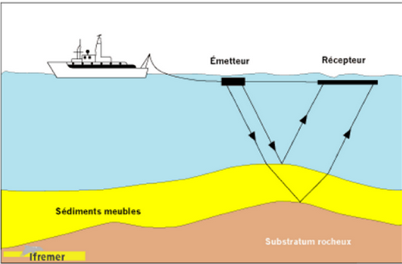
\includegraphics[width=8cm]{images/hpl_petrole.png}
            \caption{\label{pic:hpl_petrole}Étude de fond marin grâce à la sismique de réflexion.}
        \end{figure}


\subsection{Le calcul haute performance} \label{sec:supercomputer}
%%%%%%%%%%%%%%%%%%%%%%%%%%%%%%%%%%%%%%%%%%%%%%%%%%%%%%%%%%%%%%
        
        
    Aujourd'hui, presque que tout ce que nous utilisons a été simulé, à un tel point que l’avancée de nos sociétés dépend de la puissance de calcul disponible pour réaliser ces simulations. La rapidité de l'exécution des simulations numériques dépend alors de la puissance de calcul disponible pour exécuter l’application. Le domaine du \gls{hpc} est le domaine informatique qui consiste à exécuter ces applications le plus efficacement possible sur une plateforme. Celle-ci peut être un simple ordinateur personnel ou un centre de calculs dédié. De telles infrastructures sont utilisées dans de nombreux domaines dont les principaux sont la simulation numérique, la cryptographie, l'analyse de données (\textit{big data}), l’intelligence artificielle ou la sécurité. En fonction des besoins des applications (puissance de calcul, espace mémoire, stockage), mais aussi des budgets alloués, des infrastructures adaptées sont développées:
    
   \begin{enumerate}
        \item \textbf{Le supercalculateur dédié} (\textit{dedicated supercomputer}) consiste à la création d'une architecture unique qui ne sera pas répliquée. Le premier supercalculateur élaboré par Seymour Cray alors employé de l'entreprise Control Data (le CDC6600) utilisait un tel mode de conception. Il était alors l'ordinateur le plus puissant de la planète grâce à une mémoire de 131000 mots de 60 bits, une fréquence de 40 MHz et sa capacité calculatoire de $3.3 \times 10^6$ opérations par seconde. À titre de comparaison, l'ordinateur portable utilisé pour écrire ce manuscrit est capable d'exécuter plus de $10^9$ opérations par seconde. L'objectif de ce type d'infrastructure est d'être parfaitement adapté aux besoins de l'application. La conception de ces architectures étant unique, les frais de conception sont très élevés, mais cette spécificité en fait des architectures très performantes. 
        
        \item \textbf{Le commodity cluster}. L'augmentation de la vitesse des circuits ainsi que l'augmentation exponentielle du nombre de transistors des circuits a rendu les supercalculateurs dédiés très difficiles à alimenter en énergie ou à être refroidi. Il a alors fallu repenser leur architecture pour continuer à augmenter la puissance des supercalculateurs. Les \textit{commodity cluster} agrègent du matériel grand public (haut de gamme) pour former des grappes de calculs de plusieurs milliers de processeurs. La performance de ces architectures ne repose pas sur l'utilisation de matériels ultra-optimisés, mais sur l'agrégation de milliers de serveurs (noeuds de calculs) travaillant ensemble. L'Intel Paragon est un des premiers exemples de cluster construit par Intel en 1992\footnote{source: \url{https://www.top500.org/featured/systems/intel-xps-140-paragon-sandia-national-labs/\#Historical}}, qui regroupe 3680 processeurs indépendants atteignant une puissance cumulée de $143.40 \times 10^9$ \gls{FLOP}. Ce modèle de supercalculateur est le plus répandu actuellement et a permis l'élaboration des supercalculateurs les plus puissants de la planète. Ces infrastructures sont généralement développées pour des industries privées ou de grandes universités (voir \autoref{fig:hpc_bsc_super}).
        
        \item \textbf{L'informatique en nuage} (\textit{cloud computing}),  utilise le modèle \textit{System as a Service} (SAS) pour apporter aux entreprises manquant de moyens, ou de compétences, un accès à une infrastructure HPC externalisée. Les principaux avantages sont la flexibilité d'usage (adapter l'infrastructure à son besoin) ainsi que la sous-traitance de la gestion de la plateforme. L'informatique en nuage permet  à des petites structures (PME, petites universités) d'avoir accès à une ressource de calculs facilement à coûts modérés. Nous pouvons notamment citer le projet SIMSEO \cite{Saguez2016} qui a pour but de sensibiliser et d'accompagner les PME à utiliser la simulation numérique. %L'informatique en nuage permet aussi de faciliter les évolutions de matériels et permet d'utiliser les dernières technologies.
        %Le \textit{nuage} peut être implémenté de deux façons. La première est d'utiliser un nuage public où les machines sont gérées par le prestataire directement dans leur centre de données. La deuxième est d'installer un \textit{nuage} privé, le client choisi où installer la plateforme. Cette seconde solution est particulièrement recherchée par les entreprises utilisant des données sensibles et refusant qu'elles soient stockées dans un autre pays. 
        
        \item \textbf{Les grilles informatiques} (\textit{Grid Computing}) sont un regroupement de ressources informatiques à grande échelle (nationale voire internationale). Par exemple \textit{Einstein@Home} \cite{Abbott2009} est un projet de recherche mondial sur les ondes gravitationnelles  qui regroupe les ordinateurs de 50000 utilisateurs connectés à travers le monde pour analyser les données transcrites par des capteurs. En octobre 2000, l'université de Stanford a déployé un projet de calcul distribué, nommé Folding@Home \cite{Larson2009}, permettant simuler la dynamique des protéines (pliage et mouvement) impliquées dans une grande variété de maladies. Pour contribuer aux calculs, il est possible d'installer un logiciel sur son ordinateur qui effectue les calculs lorsque ce dernier n'est pas utilisé. En avril 2020, alors plus de la moitié de la population est confinée chez elle à cause de l'épidémie du COVID-19, la puissance de calcul du projet Folding@Home est utilisée pour étudier le coronavirus SARS-CoV-2 et aider au développement d'un vaccin\footnote{Coronavirus : comment votre ordinateur pourrait aider à trouver un vaccin - \url{https://www.ft.com/video/51bc9532-b08d-4129-b4db-c88ca5d42342}}. Le réseau compte plus de 2 millions de processeurs et  700 000 GPU, formant la plateforme de calcul la plus puissante de la planète ($2,5 \times 10^{18}$ opérations par seconde). 
        
    \end{enumerate}
        
        
        \begin{figure}
        \center
        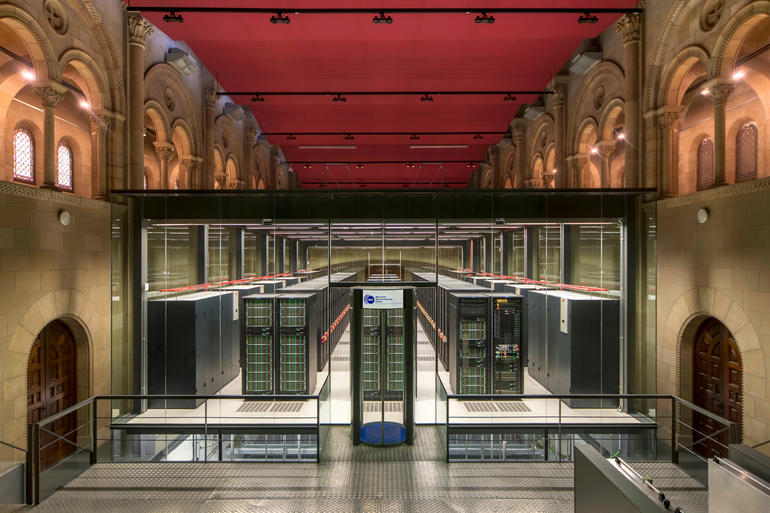
\includegraphics[width=12cm]{images/hpc_bsc_super.jpg}
        \caption{\label{fig:hpc_bsc_super} Le supercalculateur du Centre de Calcul de Barcelone (BSC) est installé dans une ancienne chapelle.}
        \end{figure}
        
        
    
        
    \subsubsection{Architecture des supercalculateurs}
    %%%%%%%%%%%%%%%%%%%%%%%%%%%%%%%%%%%%%%%%%%%%%%
    
        Les deux principales caractéristiques d'un supercalculateur sont sa capacité à calculer rapidement ainsi que sa capacité à mémoriser les informations et les résultats produits. L'architecture des supercalculateurs modernes n'est pas très différente de celle des ordinateurs classiques. La puissance d'une telle plateforme vient seulement de l'agrégation de centaines de ressources de calculs, capables de travailler ensemble pour résoudre un problème complexe. Le domaine du HPC consiste à exécuter efficacement des applications sur de telles architectures. Pour cela, l'infrastructure utilisée doit gérer l'équilibrage de la charge de calcul sur les différentes ressources disponibles ainsi que la gestion des communications entre les ressources. Un supercalculateur moderne possède généralement les cinq parties suivantes:
      
        \begin{enumerate}
        
            \item \textbf{Les serveurs} utilisés dans un supercalculateur possèdent un ou plusieurs processeurs. Comme un ordinateur classique, chaque processeur est relié à la mémoire et au stockage (voir \autoref{fig:motherboard}). En fonction des configurations, chaque serveur peut être agrémenté d'un ou plusieurs accélérateurs (GPU). La principale différence avec un ordinateur classique, autre que la puissance des matériels utilisés, vient du système d'interconnexion (voir \autoref{fig:dl360_back}). Les serveurs doivent pouvoir échanger des informations pour se synchroniser ou partager des résultats entre eux et accéder au stockage (voir \autoref{sec:edl_interco}).
        
                \begin{figure}[t!]
                    \centering
                    \begin{subfigure}[t]{0.48\textwidth}
                        \centering
                        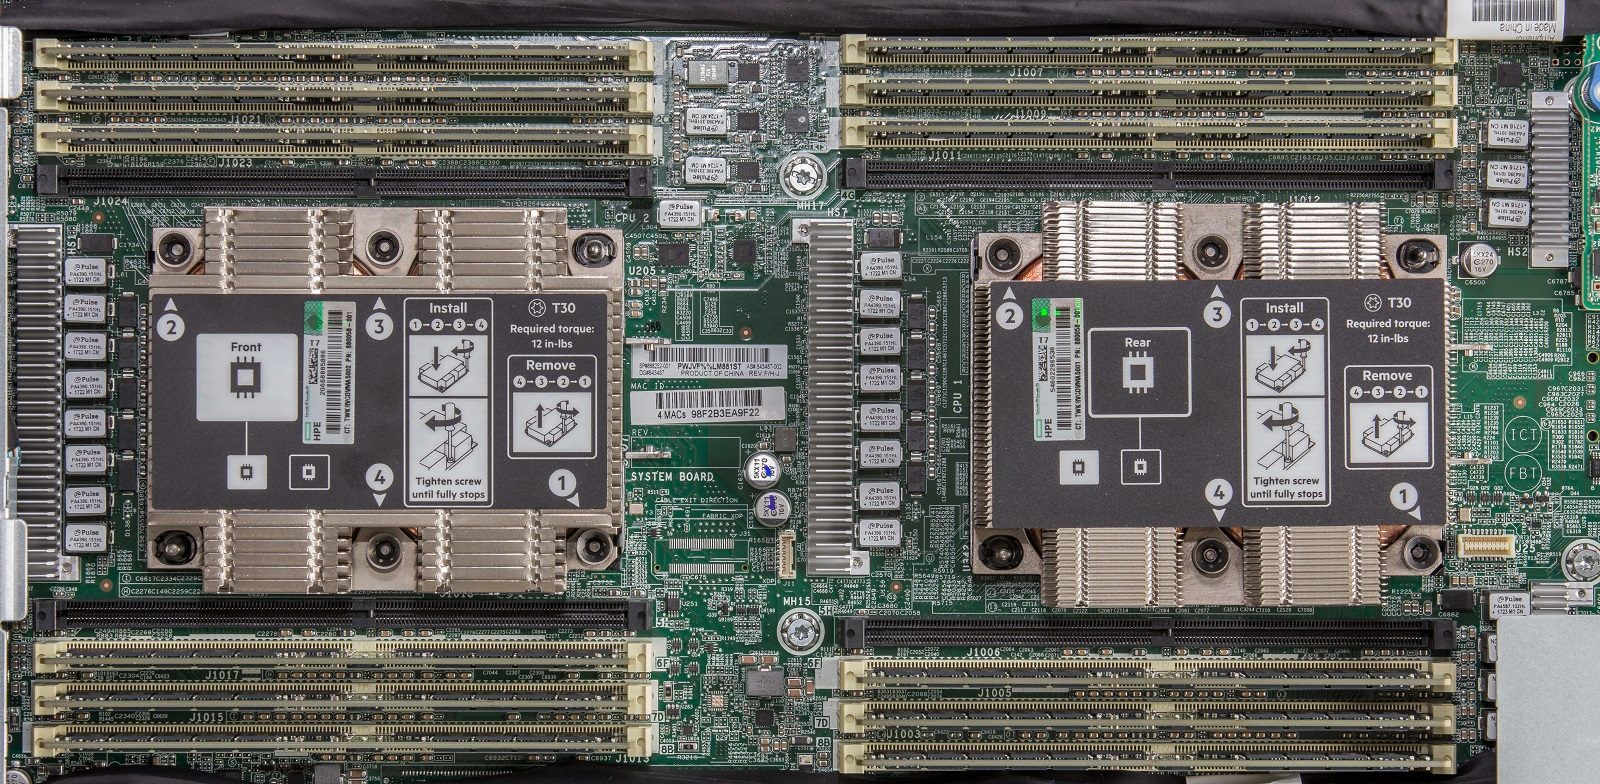
\includegraphics[width=.9\linewidth]{images/motherboard.jpg}
                        \caption{\label{fig:motherboard}Carte mère d'un serveur possédant deux processeurs.}
                    \end{subfigure}\hfill
                \begin{subfigure}[t]{0.48\textwidth}
                        \centering
                        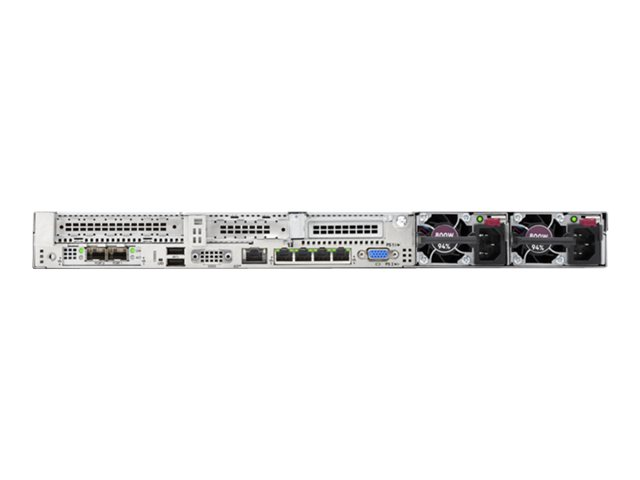
\includegraphics[width=\linewidth]{images/dl360_back.jpg}
                        \caption{Vu arrière d'un serveur exposant les différentes interfaces de connexion.\label{fig:dl360_back}}
                    \end{subfigure}
                    \caption{Exemple d'un serveur utilisé dans les supercalculateurs.}
                    \label{pic_pi_rect}
                \end{figure}
    
            \item \textbf{Les accélérateurs}. Un principe fondamental des processeurs énoncés par Von Neumann était leur universalité. Leur faculté à exécuter tout type de code est à la fois une force, mais aussi une de leur plus grande faiblesse. Ils sont très peu efficaces, en temps et en énergie, pour résoudre certains types de calculs tels que les traitements de signaux ou d'objets géométriques. Pour accélérer certaines classes d'applications, des architectures spécialisées, appelées accélérateurs, sont utilisés pour améliorer la performance et la consommation énergétique des infrastructures. Les applications d'intelligence artificielle utilisent des \gls{GPU} pour accélérer l'entraînement des modèles. D'autres accélérateurs comme les \gls{FPGA} peuvent être utilisés pour accélérer la phase d'inférence.
            
            :
                \begin{itemize}
    
                    \item\textbf{Les GPU}. À l'origine, les \gls{GPU} étaient destinés au domaine des jeux vidéo et aux calculs de rendus graphiques. Suite à leur utilisation pour d'autres applications que le rendu graphique, ces accélérateurs sont aussi nommés GP-GPU pour \textit{general purpose GPU}. À l'inverse des processeurs, les GPU sont composés de nombreux coeurs (plusieurs centaines). Ceux-ci sont moins complexes et performants que les coeurs de processeur, mais leur nombre les rend particulièrement efficaces pour certaines applications. La \autoref{fig:CPUvsGPU} compare l'évolution des performances des GPU avec celles des CPU de même génération. On remarque l'écart significatif séparant leur performance. Cependant, la figure représente la performance théorique des architectures et il est rare que les applications s'en approchent. 
                    Actuellement, il existe deux fournisseurs principaux de GPU (Nvidia et AMD) qui ont pu bénéficier de leur longue expérience dans le domaine du jeu vidéo. La première nécessite l'utilisation de langage propriétaire (\verb|CUDA|) quand la deuxième peut être programmée grâce au langage \verb|OpenCL|. Le principal avantage de \verb|CUDA| est de pouvoir utiliser des librairies optimisées par NVIDIA pour ses plateformes pour différents domaines (algèbre linéaire (cuBLAS, CUSPARSE), analyse de signal (cuFFT), apprentissage machine (cuDNN, TensorFlow). 
                    \verb|OpenCL| a été initié par Apple et est maintenant maintenu par le groupe Khronos. C'est un standard ouvert et libre de droits permettant l'exécution de codes sur différentes plateformes. Une application utilisant \verb|OpenCL| pourra être, en théorie, facilement portée sur d'autres architectures (CPU, FPGA, DSP). 
                    
                        \begin{figure}
                        \center
                        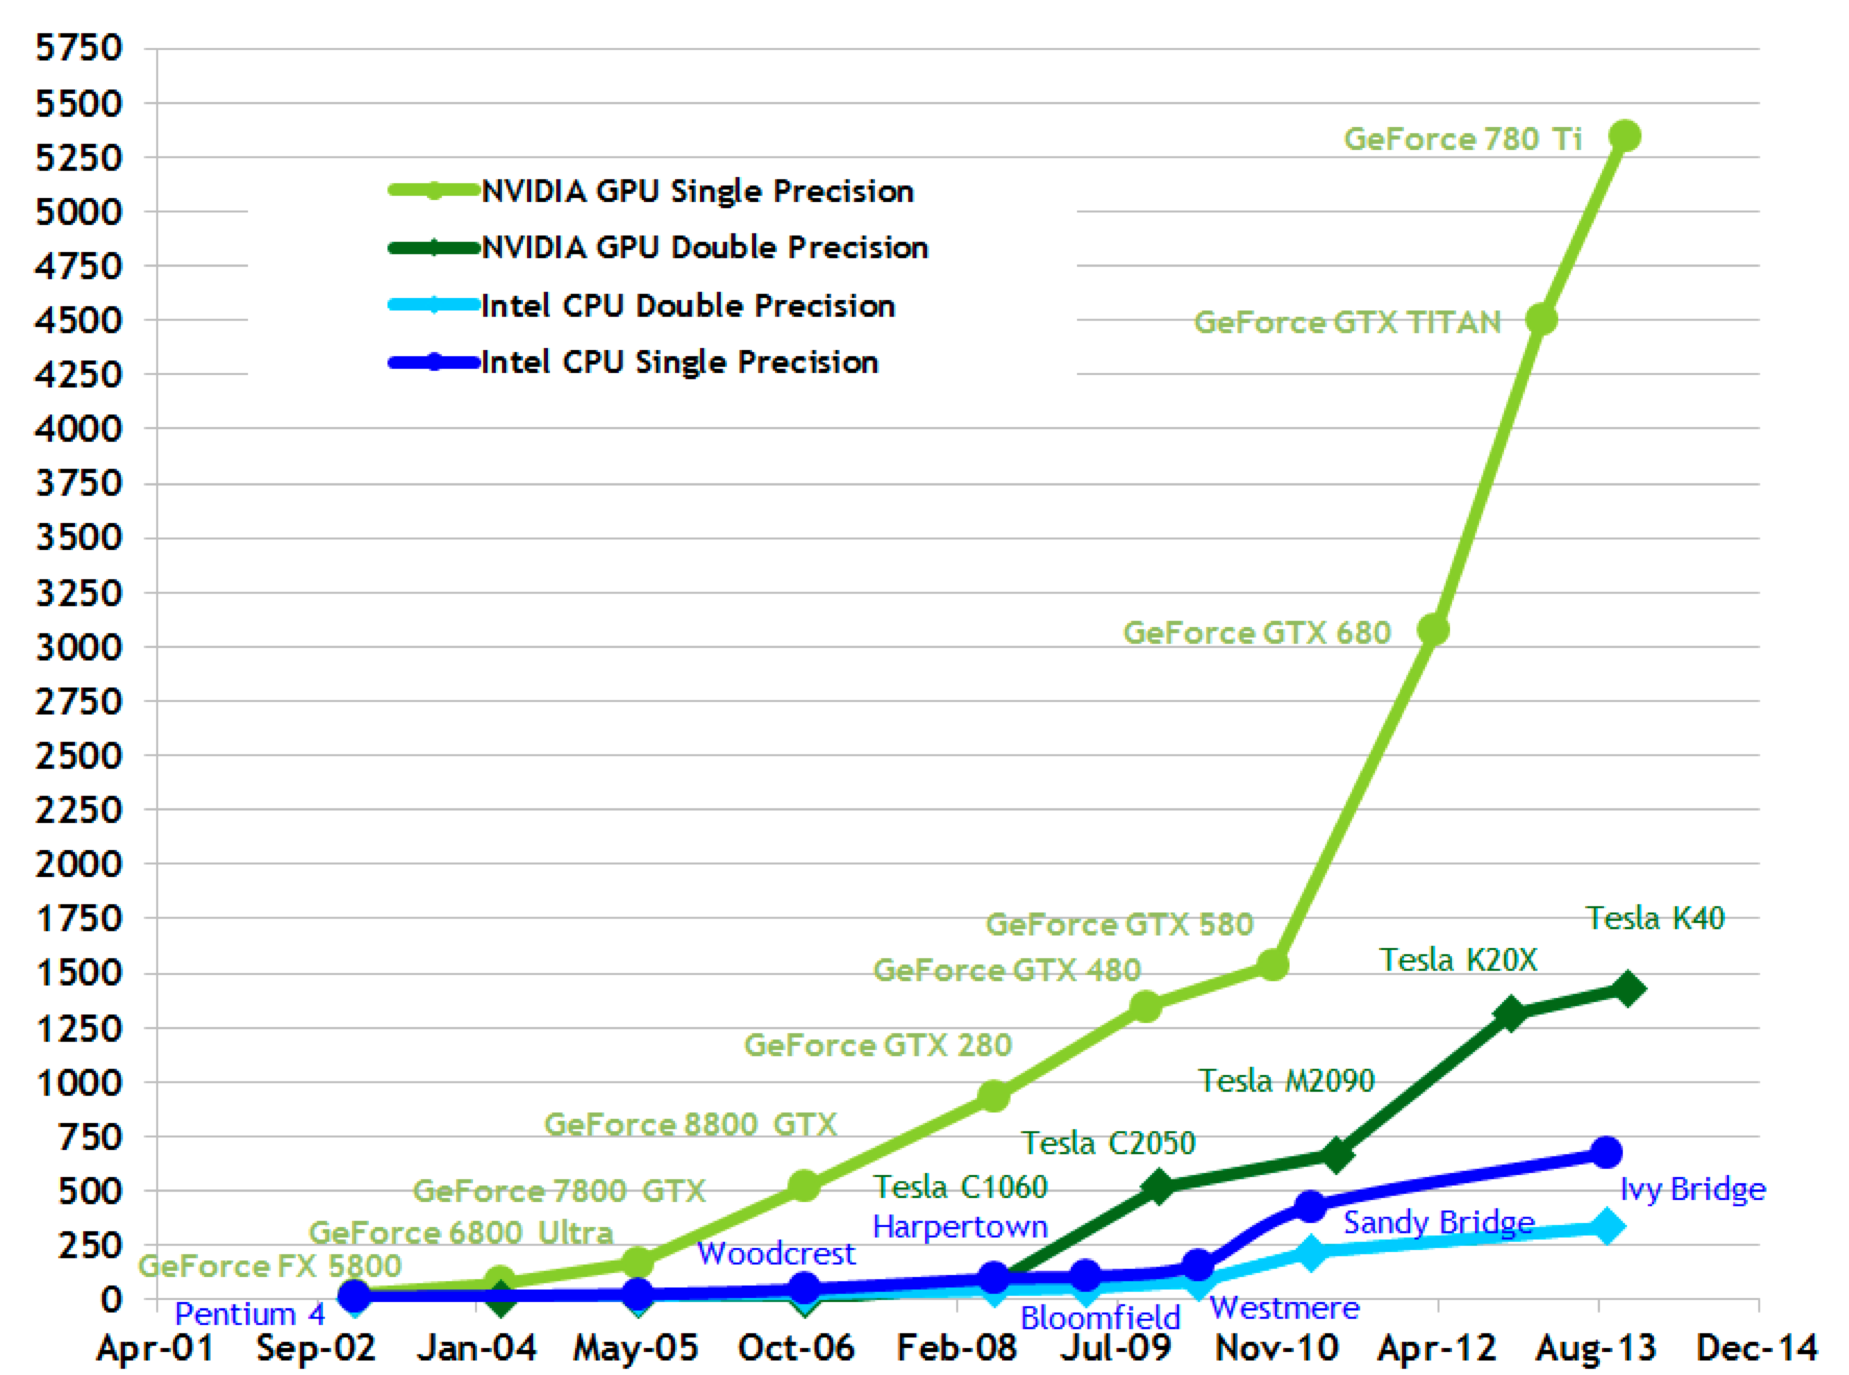
\includegraphics[width=10cm]{images/CPUvsGPU.png}
                        \caption{\label{fig:CPUvsGPU} Comparaison des performances entre différentes générations de CPU et de GPU}
                        \end{figure}
                     
                    
                    
                    
                    %Cependant, pour des applications particulièrement adaptées, le GPU n'a pas d'équivalent actuellement en termes de performance. La performance du bus mémoire d'un GPU est elle aussi bien supérieure, rendant ces architectures d'autant plus intéressantes pour les codes dont la performance est limitée par le système mémoire. 
                    
                    %Acutellement, le développement ou le portage d'applications pour pouvoir être exécutées sur ces architectures demande un investissement conséquent. L'architecture spécifique des GPU nécessite au programmeur de présenter explicitement la parallélisation d'un noyau. De plus, le GPU possédant son propre espace mémoire, le programmeur doit gérer explicitement les transferts entre celle-ci et la mémoire centrale du serveur.
                    %De nombreux travaux essaient de combler cette difficulté. La plus notable étant surement OpenACC. Crée en 2011, cet outil permet d'annoter le code source d'une application à l'aide de \verb|#pragma| pour indiquer au compilateur les zones parallélisable. Avec un effort raisonable, des performances proches des performances atteinte en utilisant \verb|CUDA| peuvent être atteinte. 
                        
                    \item\textbf{Les FPGA.}  Les \gls{FPGA} sont de simples circuits intégrés qui contiennent des portes logiques pouvant être programmées pour la réalisation d'un circuit. 
                    Les méthodes traditionnelles de développement sur FPGA nécessitent la conception d'une architecture matérielle utilisant un langage adapté comme le Hardware Description Language (HDL). Pour ce faire, le développeur doit concevoir les chemins de données ainsi que la logique de contrôle. Il s'agit d'un processus de développement fastidieux et complexe qui peut entraver leur adoption. Les FPGA les plus récents peuvent être programmés à l'aide d'\verb|OpenCL|.
                    Implémenter un circuit à l'aide d'un FPGA peut fournir une efficacité énergétique légèrement inférieure à celle obtenue par une implémentation d'un \gls{asic}. Cependant, le fait que les FPGA soient programmables leur donne un avantage sur les ASIC, car le même matériel peut être reprogrammé en un nouveau circuit. Le temps de reprogrammation étant relativement faible, il peut être intéressant de reprogrammer le FPGA plusieurs fois pour les différentes phases de l'application. Cependant, la complexité de programmation des FPGA et leur prix très élevé sont les principaux freins pour leur adoption dans les supercalculateurs.        
                    
                    \item\textbf{Les DSP}. Les \gls{dsp} sont adaptés pour les opérations de convolution et de filtrage très utilisés par les algorithmes d'analyse de signal. Généralement contraints par leur consommation électrique (matériel embarqué, smartphone, robotique), les DSP utilisent des fréquences plus basses que les processeurs. Du fait de leur implémentation d'opérations optimisées, elles sont plus efficaces que les architectures standards pour ces applications. Les opérations de filtrage nécessitent, pour être optimales, d'avoir accès à chaque cycle à une instruction et deux opérandes. Les architectures Harvard utilisées par les DSP (voir \autoref{sec:harvard}) sont alors plus optimales pour ce type d'exécution grâce à leurs deux bus d'accès (données et instructions).
                     
             \end{itemize}
             
             
                %Étant architecturalement adaptés à certains algorithmes, les accélérateurs sont généralement plus efficaces énergétiquement. Dans un contexte où l'énergie est une pression majeure, leur utilisation est d'autant plus pertinente. Pour pouvoir être utilisées et obtenir les meilleures performances, les applications doivent être adaptées. Cela impose aux développeurs d'apporter des transformations à leur code, d'utiliser un nouveau compilateur ou même un autre langage. Ces transformations peuvent réduire la portabilité de l'application, notamment quand un langage propriétaire, tel que \verb|CUDA| est utilisé.  Un accélérateur peut être adapté à la résolution d'une partie de l'application, mais peut être très inefficace pour le reste. Cela rend le choix de l'accélérateur difficile, car l'investissement (budget et modification de code) doit être rentable pour l'utilisateur.
           
                  
                    
            \item \textbf{Le stockage}. Les applications de calculs intensifs ont besoin d'avoir accès à une grande capacité de stockage. Certaines applications utilisent des jeux de données dépassant de plusieurs facteurs la capacité de stockage du serveur. Ceux-ci doivent donc être stockés à l'extérieur du serveur. D'autres applications peuvent produire des résultats ne pouvant pas non plus être stockés sur les serveurs. Pour ces deux utilisations, un supercalculateur doit posséder un stockage avec les meilleures caractéristiques possible: latences, débits, fiabilité. Suivant le type d'application, la priorité n'est pas la même.
            
            
                   
            \item \textbf{L'interconnexion}\label{sec:edl_interco} Les applications étant réparties sur différents serveurs, ces derniers ont besoin d'être interconnectés pour s'échanger des informations (résultats temporaires, instructions) ou pour se synchroniser. Le système d'interconnexion participe à une part importante de la performance finale. Le matériel utilisé doit donc être adapté aux besoins de l'application. Suivant sa nature, une application bénéficie d'un réseau avec une faible latence et/ou un débit élevé.
            La latence inclut le temps nécessaire aux routeurs pour rediriger le message au destinataire. Pour cela, la structure des routeurs doit être bien pensée pour réduire le nombre de \textit{sauts} de chaque échange, c'est-à-dire le nombre d'intermédiaires pour aller de l'expéditeur au destinataire. La figure \ref{pic_topologie} montre un exemple de topologie et l'impact qu'elle a sur la latence des communications qui peut être multipliée par deux suivant le destinataire du noeud $A$. Cette structure (ou topologie) doit s'assurer d'éviter tout risque de congestion afin qu'une partie de réseau ne soit pas trop sollicitée ce qui créerait des baisses de performances.    
            Différentes technologies sont ainsi développées pour répondre aux différents besoins (et différents budgets). Les technologies dites \verb|10GbE| (\textit{10 Gigabit Ethernet}), basées sur TCP, permettent d'échanger des informations pour un débit allant jusqu'à 10 Gb/s. Ce réseau peut être implémenté à l'aide de câble en cuivre ou de fibre optique. Un second protocole appelé Infiniband permet d'atteindre des débits plus élevés tout en assurant la réussite des transferts. En fonction de l'application utilisée, le choix de la technologie réseau utilisée peut avoir un fort impact sur ses performances \cite{Council2009}.
                Aussi, l'efficacité du réseau ne dépend pas seulement du matériel, la partie logiciel est tout aussi importante comme la complexité des protocoles ou la performance des algorithmes de routage.
                
                    \begin{figure}
                    \center
                    \includegraphics[width=6cm]{images/Chapitre1/TopologieReseau.png}
                    \caption{\label{pic_topologie} Exemple d'une topologie d'un cluster. Si le serveur A veut envoyer un message à B, il devra effectuer 4 sauts (ou \textit{hop}).}
                    \end{figure}
          
    
            \item \textbf{Le système de refroidissement}. La puissance électrique utilisée par les différents matériels est dissipée sous forme de chaleur. Il n'est pas rare qu'une armoire (un \textit{rack}) consomme à elle toute seule plus de 50 kW. Un supercalculateur doit donc posséder un système de refroidissement performant pour éviter les surchauffes des composants. En effet, celles-ci peuvent provoquer un ralentissement des matériels (fréquences des processeurs) ou même les détériorer. De nombreuses technologies ont été développées pour améliorer le rendement des systèmes de refroidissement tels que le refroidissement liquide ou l'immersion des composants dans des bains d'huile.
        \end{enumerate}


\subsection{Programmation parallèle et performance des supercalculateurs}      
\label{sec:prog_parallele}
%%%%%%%%%%%%%%%%%%%%%%%%%%%%%%%%%%%%%%%%%%%%%%%%%%%%%%%%%%%%%%%%%%%

    \subsubsection{Le calcul parallèle}\label{sec:exemple_pi}
    %%%%%%%%%%%%%%%%%%%%%%%%%%%%%%%%%%%%%%%%%%%%%%%%%%%%%%%%%%%%%%%%%%%
        
        L'agrégation de milliers de ressources de calcul (processeurs, accélérateurs) a pour objectif d'accélérer l'exécution d'applications qui ne pourraient pas être réalisées par une seule d'entre elles dans un temps raisonnable. Le travail des programmeurs est alors de diviser ce problème complexe en sous-problèmes indépendants, pouvant être résolus simultanément par les différentes ressources. Cette méthode de résolution, appelée calcul parallèle, regroupe l'ensemble de moyens, logiciels et matériels qui permettent de réduire le temps de calcul d'un programme en répartissant la charge de travail.
       
        Pour illustrer la nécessité d'avoir recours aux techniques de calcul parallèle, nous présentons un exemple simple permettant de réaliser l'approximation de $\pi$ par le calcul de l'intégrale suivante:
        \begin{equation}
        \label{eq_pi}
        \int_{0}^{1} \frac{4.0}{1 + x^{2}}
        \end{equation}
        
        %ILLUSTRATION PI    
        \begin{figure}[t!]
            \centering
            \begin{subfigure}[t]{0.5\textwidth}
                \centering
                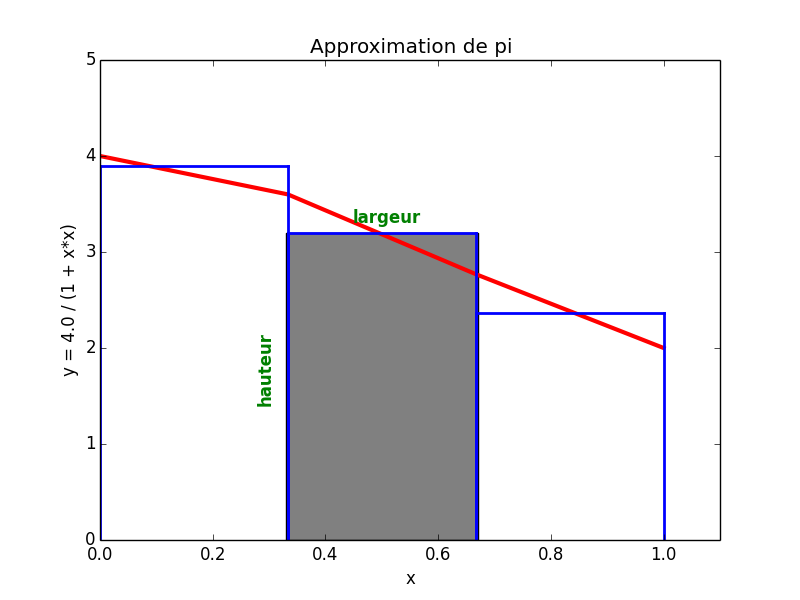
\includegraphics[height=2.2in]{images/Chapitre1/pic_pi_rect_1.png}
                \caption{\label{pic_pi_1} Approximation avec 4 rectangles}
            \end{subfigure}%
        \begin{subfigure}[t]{0.5\textwidth}
                \centering
                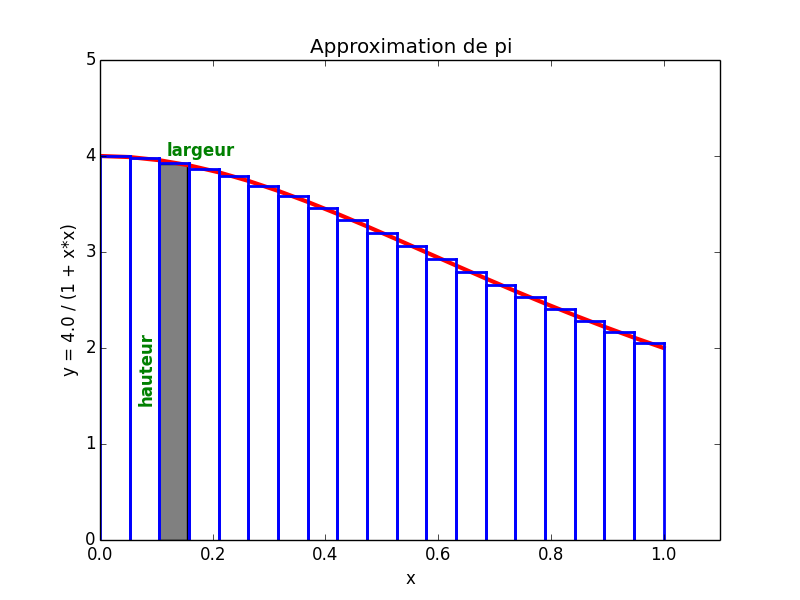
\includegraphics[height=2.2in]{images/Chapitre1/pic_pi_rect_2.png}
                \caption{\label{pic_pi_2} Approximation avec 14 rectangles}
            \end{subfigure}
            \caption{\label{pic_pi_rect} Méthode des rectangles: exemple de deux exécutions de l'algorithme avec un nombre de rectangles différents.}
            
        \end{figure}
            
        Calculer une intégrale revient à calculer l'aire formée par cette courbe et l'axe des abscisses dans le domaine étudié, ici $[0,1]$. Cette surface peut être approximée par la méthode des rectangles (ou trapèze). Cette méthode revient à dessiner des rectangles sous la courbe (voir \autoref{pic_pi_rect}). La surface de ces derniers pouvant être calculée, il est alors possible d'approcher l'intégrale donnée dans l'\autoref{eq_pi} à l'aide du code présenté dans l'extrait de code suivant:
        
        %ALGO PI
        \begin{lstlisting}[language=C, caption=Implémentation de l'algorithme de calcul d'intégrale par la méthode des rectangles, float,floatplacement=H]
double x, largeur, hauteur, pi = 0.0;

int num_steps = 4;
int num_steps = 14;

largeur = 1.0 / num_steps;

for (int i = 0; i < num_steps; ++i) {
    x =  (i) * largeur;
    hauteur = ( 4.0/(1.0+x*x));
    pi += largeur * hauteur;
}

cout << "Valeur de pi: " << pi << endl;
\end{lstlisting}
    
         Nous remarquons sur la \autoref{pic_pi_1}, qu'avec l'utilisation de quatre rectangles, la surface des rectangles ne correspond pas exactement à la courbe à approcher. Ces erreurs affectent la précision de notre programme qui affiche une valeur de $\pi = 3.38$. La \autoref{pic_pi_2} présente le même programme qui utilise 14 rectangles. Les rectangles sont alors plus fidèles à la courbe et le programme calcule une valeur de $\pi = 3.21$.
        Nous présentons cet exemple simpliste pour illustrer le besoin de puissance de calcul pour réaliser des simulations précises:
        \begin{itemize}
            \item La précision du calcul dépend du nombre de rectangles choisi. Plus le nombre de rectangles utilisés est grand, plus la précision augmente. Cependant, augmenter le nombre de rectangles à calculer augmente le nombre d'opérations nécessaires à réaliser. 
            
            \item Pour accélérer le calcul de cette application, le calcul des différents rectangles doit être réparti entre les ressources de calcul. À la fin de l'exécution, un processus s'occupe de récolter et additionner les différents résultats.
            
            \item La capacité d'une application à utiliser des ressources parallèles n'est pas automatique. Une transformation du code doit être réalisée de manière explicite (par le programmeur) ou implicite (par le compilateur).
        \end{itemize}
        
    \subsubsection{Niveau de parallélisme des supercalculateurs}
    %%%%%%%%%%%%%%%%%%%%%%%%%%%%%%%%%%%%%%%%%%%%%%%%%%%%%%%%%%%%%%
    
        La performance d'une application parallèle dépend donc du nombre et de la performance des ressources pouvant travailler simultanément pour la résolution du problème. La tâche des programmeurs est d'adapter le code pour répartir l'application sur les différentes ressources disponibles. Ce travail est difficile, car le parallélisme est présent à plusieurs niveaux dans un supercalculateur.
        
        
        \paragraph{Taxonomie de Flynn.}
             Les différentes formes de parallélisme ont été regroupées en quatre classes appelées taxonomie de Flynn \cite{Flynn2011} (voir \autoref{fig:flynn}). Ces classes permettent de caractériser les architectures en fonction de l'indépendance ou non des instructions et des données. La classe \verb=SISD= représente les architectures classiques n'exécutant qu'une instruction sur une donnée à la fois. 
            La classe \verb=SIMD= regroupe les architectures vectorielles exécutant une instruction sur plusieurs données à la fois (voir \autoref{sec:cpu_vectoriel}). La classe d'architecture \verb|MISD| exécute des instructions différentes sur le même jeu de données. Les processeurs capables d'exécuter des instructions réalisant \gls{FMA}, peuvent être considérées comme telles. Une instruction FMA permet de réaliser une addition et une multiplication sur une même donnée. Le processeur ASIC présent dans les voitures connectées peut par exemple exécuter deux algorithmes différents pour s'assurer de la validité d'une décision à prendre. La dernière classe \verb|MIMD| représente des architectures exécutant plusieurs instructions sur plusieurs données à la fois. Un serveur possédant plusieurs processeurs est un exemple d'architecture \verb|MIMD|. 
            
            \begin{figure}
            \center
            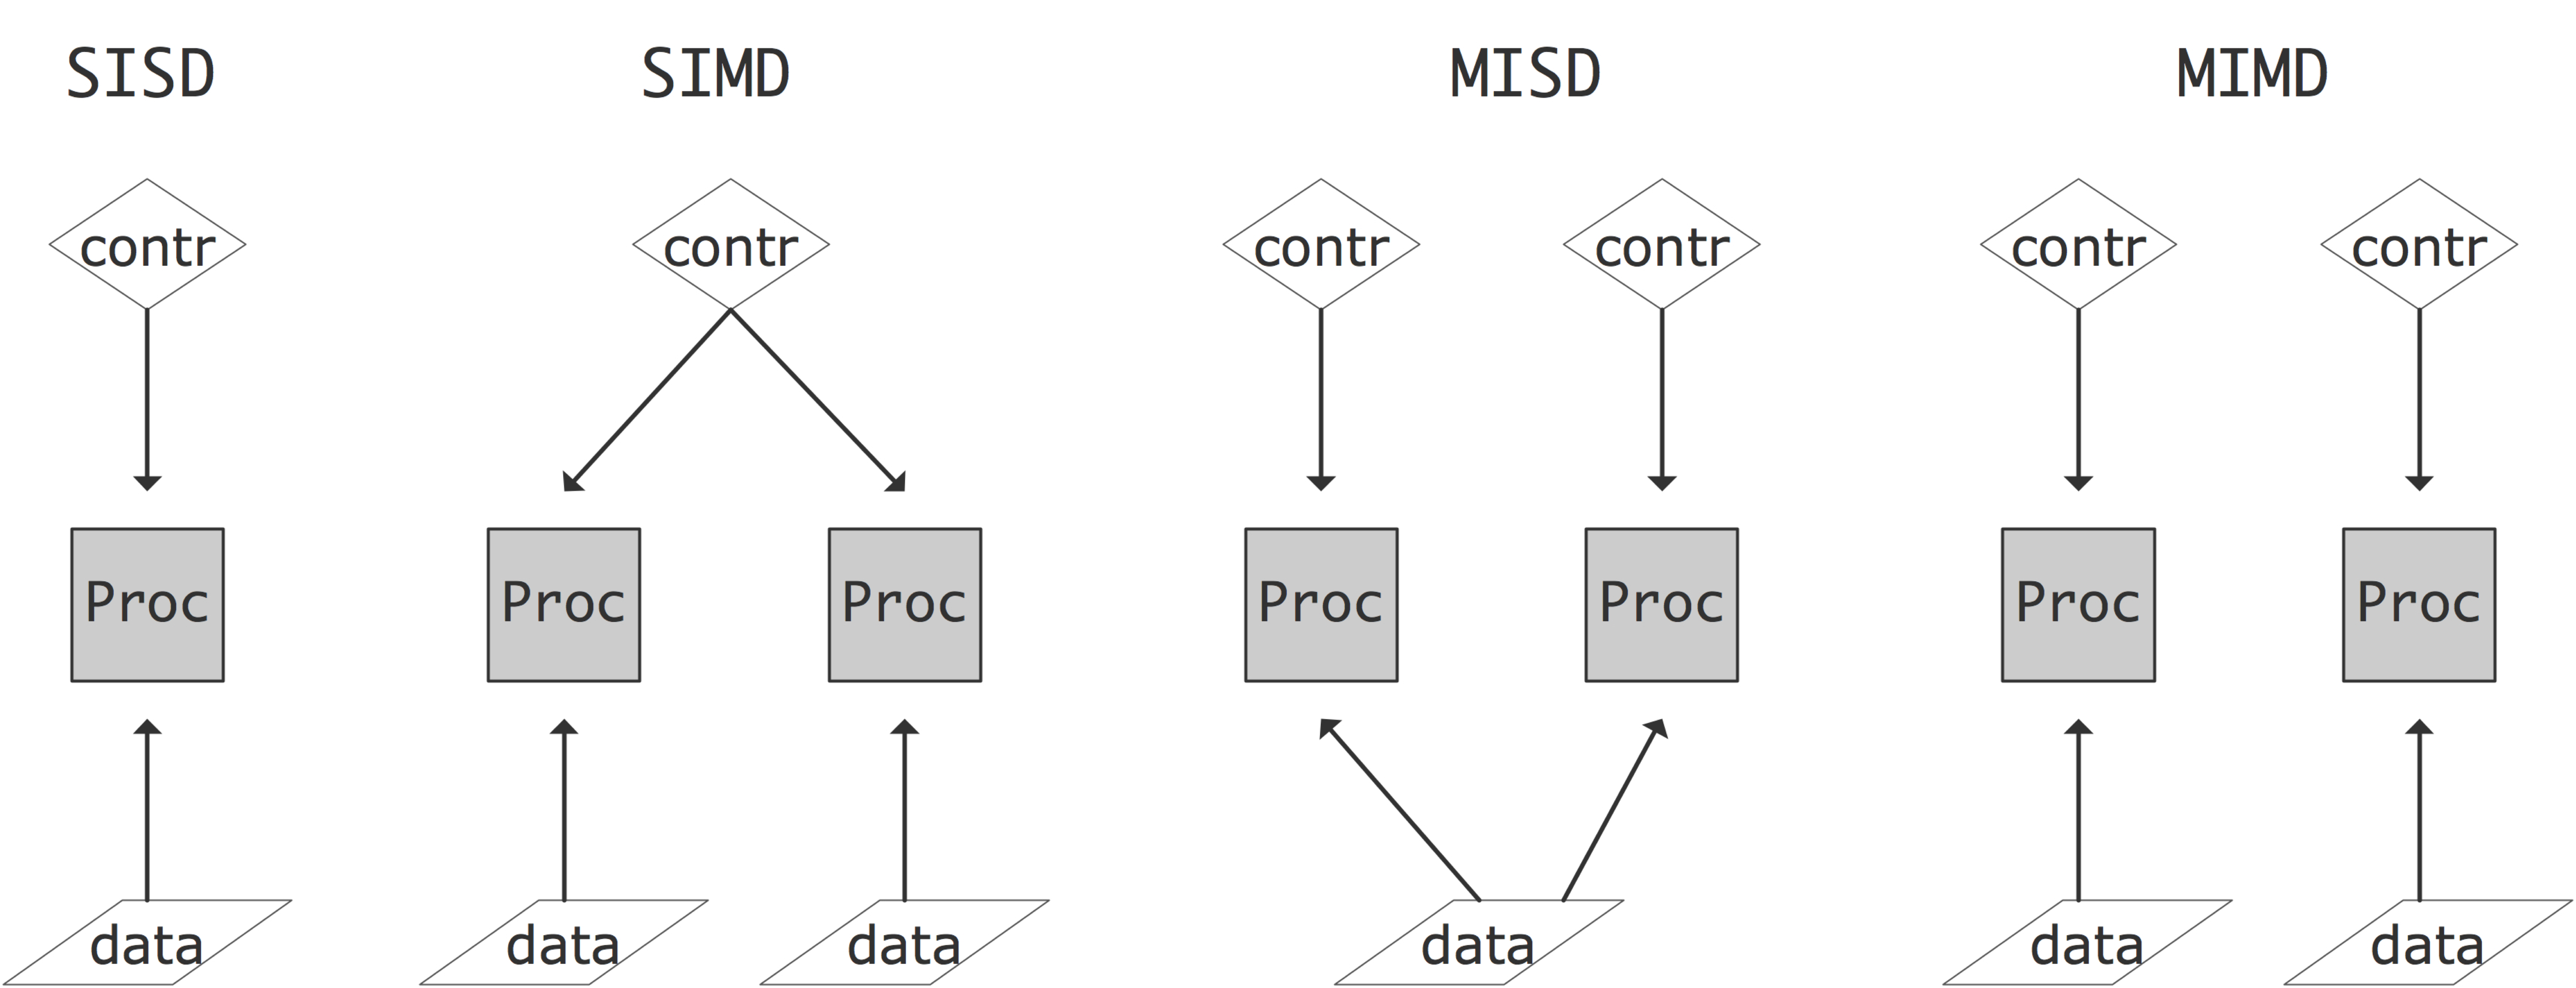
\includegraphics[width=12cm]{images/flynn.png}
            \caption{\label{fig:flynn} Les quatre classes de la taxonomie de Flynn (graphique extrait de \cite{Eijkhout2013})}
            \end{figure}
            

        \paragraph{Niveaux de parallélisme d'un supercalculateur.}
            La \autoref{fig:parallele_hpc} représente les principaux niveaux de parallélisme d'un supercalculateur. Le  niveau $1$ concerne les serveurs, reliés par un système d'interconnexion. Différentes tâches peuvent être assignées à chaque noeud qui peuvent communiquer entre eux pour se synchroniser ou partager des résultats. Le niveau $2$ concerne le parallélisme des processeurs (ainsi que des accélérateurs si le serveur en possède). En fonction des tâches à réaliser et des caractéristiques des ressources de calculs, les tâches peuvent être réparties pour être exécutées. Le niveau $3$ est situé dans les processeurs et concerne l'utilisation de processeurs multicoeurs. Le niveau $4$ est lié aux processeurs superscalaires possédant plusieurs pipelines (voir \autoref{sec:pipeline}). Le dernier niveau de parallélisme concerne les unités de calcul vectorielles des processeurs qui peuvent exécuter une instruction sur plusieurs données simultanément (voir \autoref{sec:fpu}).
            
            \begin{figure}
                \center
                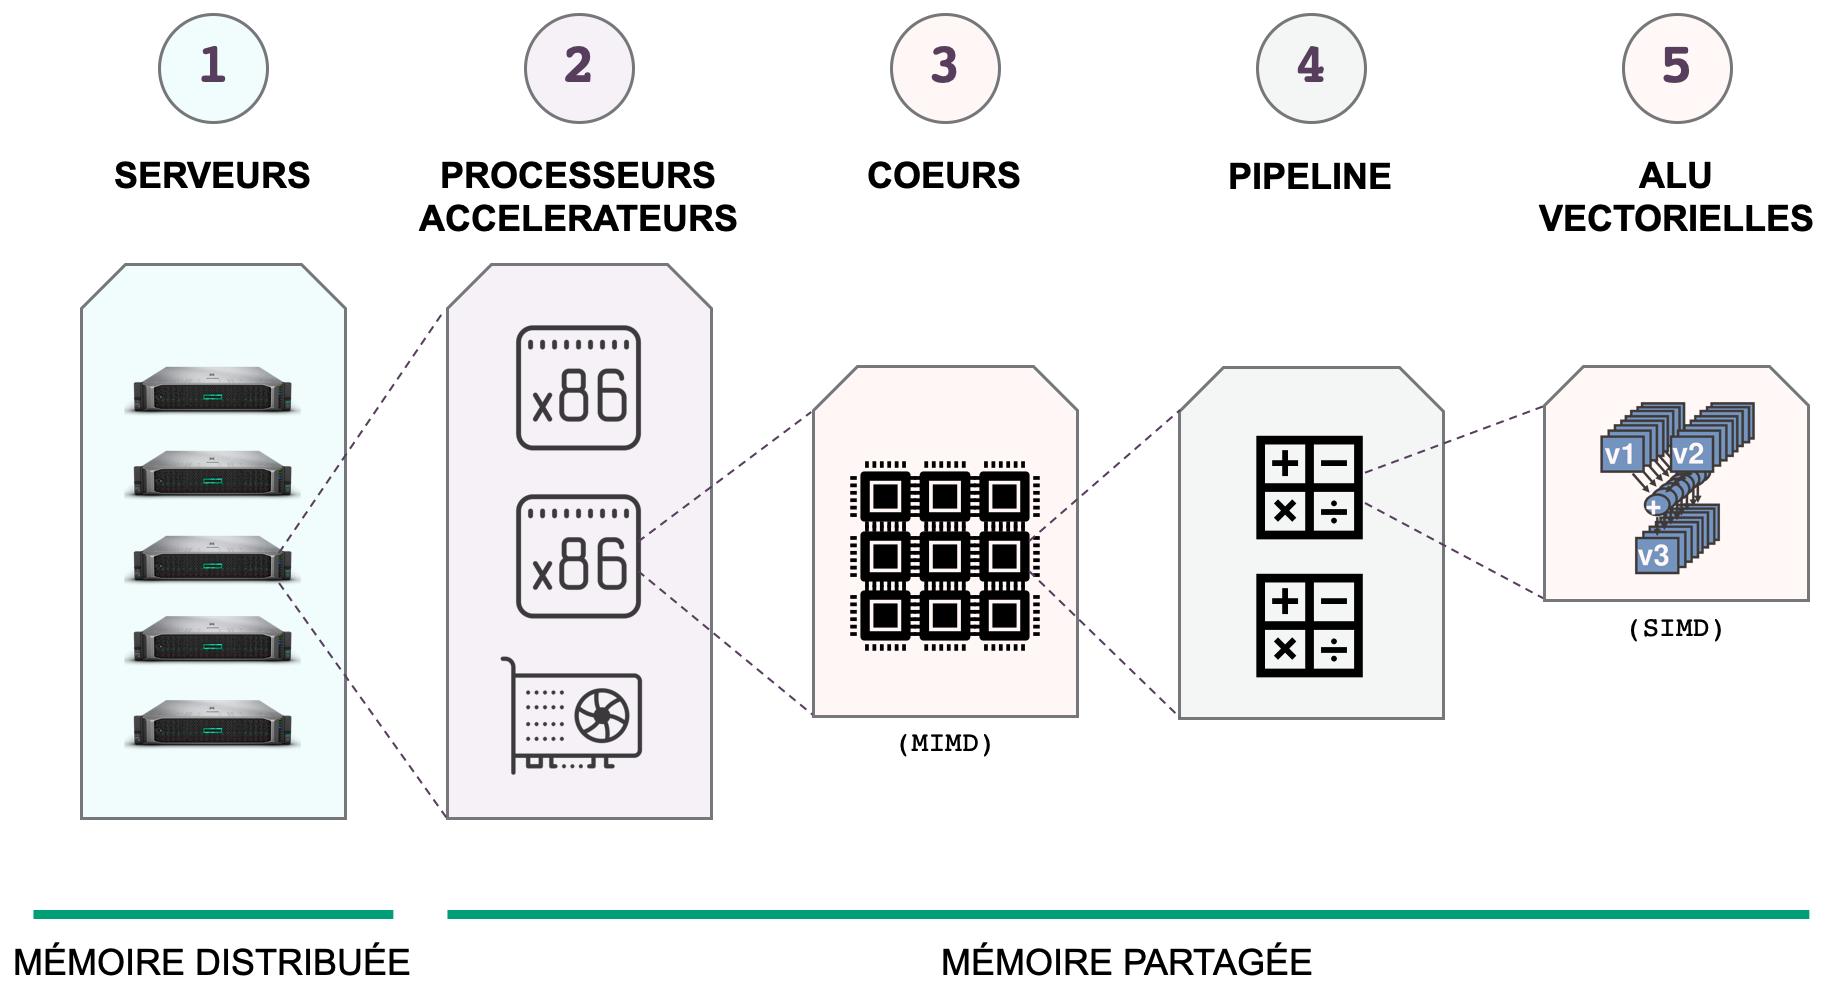
\includegraphics[width=14cm]{images/parallele_hpc.png}
                \caption{\label{fig:parallele_hpc} Différents niveaux de parallélisme dans un supercalculateur. Les processeurs MIMD sont capables d'exécuter plusieurs instructions sur plusieurs données grâce à l'utilisation de multiple coeurs. Les unités arithmétiques et logiques (ALU) peuvent exécuter une instruction sur plusieurs données à la fois (MIMD) grâce aux instructions vectorielles.}
            \end{figure}
            
            Pour maximiser le nombre d'instructions pouvant être exécutées sur un supercalculateur, (\textit{Instruction Level Parallelism} (ILP)), différentes méthodes existent. Le niveau le plus haut consiste à exécuter des applications indépendantes permettant de saturer l'utilisation de la plateforme (\textit{Job Level Parallelism}). Une même application peut être découpée en tâches qui peuvent être exécutées en parallèle (\textit{Task Level Parallelism} (TLP) \cite{Kambadur2009}). Lorsque la nature du code le permet, une instruction peut être exécutée sur plusieurs données simultanément (\textit{Data Level Parallelism}(DLP) \cite{Espasa1997}).

    \subsubsection{Paradigme de programmation}
    %%%%%%%%%%%%%%%%%%%%%%%%%%%%%%%%%%%%%%%%%%%%%%%%%%%%%%%%%%%%%%
       
        Pour pouvoir bénéficier des ressources de calculs disponibles, le programmeur doit adapter certaines parties du code. Les niveaux de parallélisme les plus bas (pipeline et ALU) sont gérés par le matériel sans intervention de l'utilisateur. Par exemple, lorsque le compilateur génère des instructions vectorielles, l'unité de calcul s'occupe seule de leur exécution. Cependant, le programmeur doit connaître les détails de la microarchitecture pour développer du code pouvant profiter du parallélisme.  Il peut par exemple adapter la structure de son code pour permettre au compilateur de présenter plusieurs instructions au module d'exécution dans le désordre (voir \aref{sec:out_of_order}) permettant ainsi d'optimiser l'utilisation des pipelines (voir \aref{sec:pipeline}) présents dans les processeurs superscalaires (voir \aref{sec:superscalar}).
        
        Pour bénéficier des niveaux $1$, $2$ et $3$ (voir \autoref{fig:parallele_hpc}), deux paradigmes fondamentaux de la programmation parallèle peuvent être utilisés: la programmation à mémoire partagée ou à mémoire distribuée. La principale distinction entre ces deux paradigmes est le partage ou non d'un espace mémoire entre les ressources utilisées (voir \autoref{fig:edl_ditribue_partage}). 
        
            \begin{figure}
                \center
                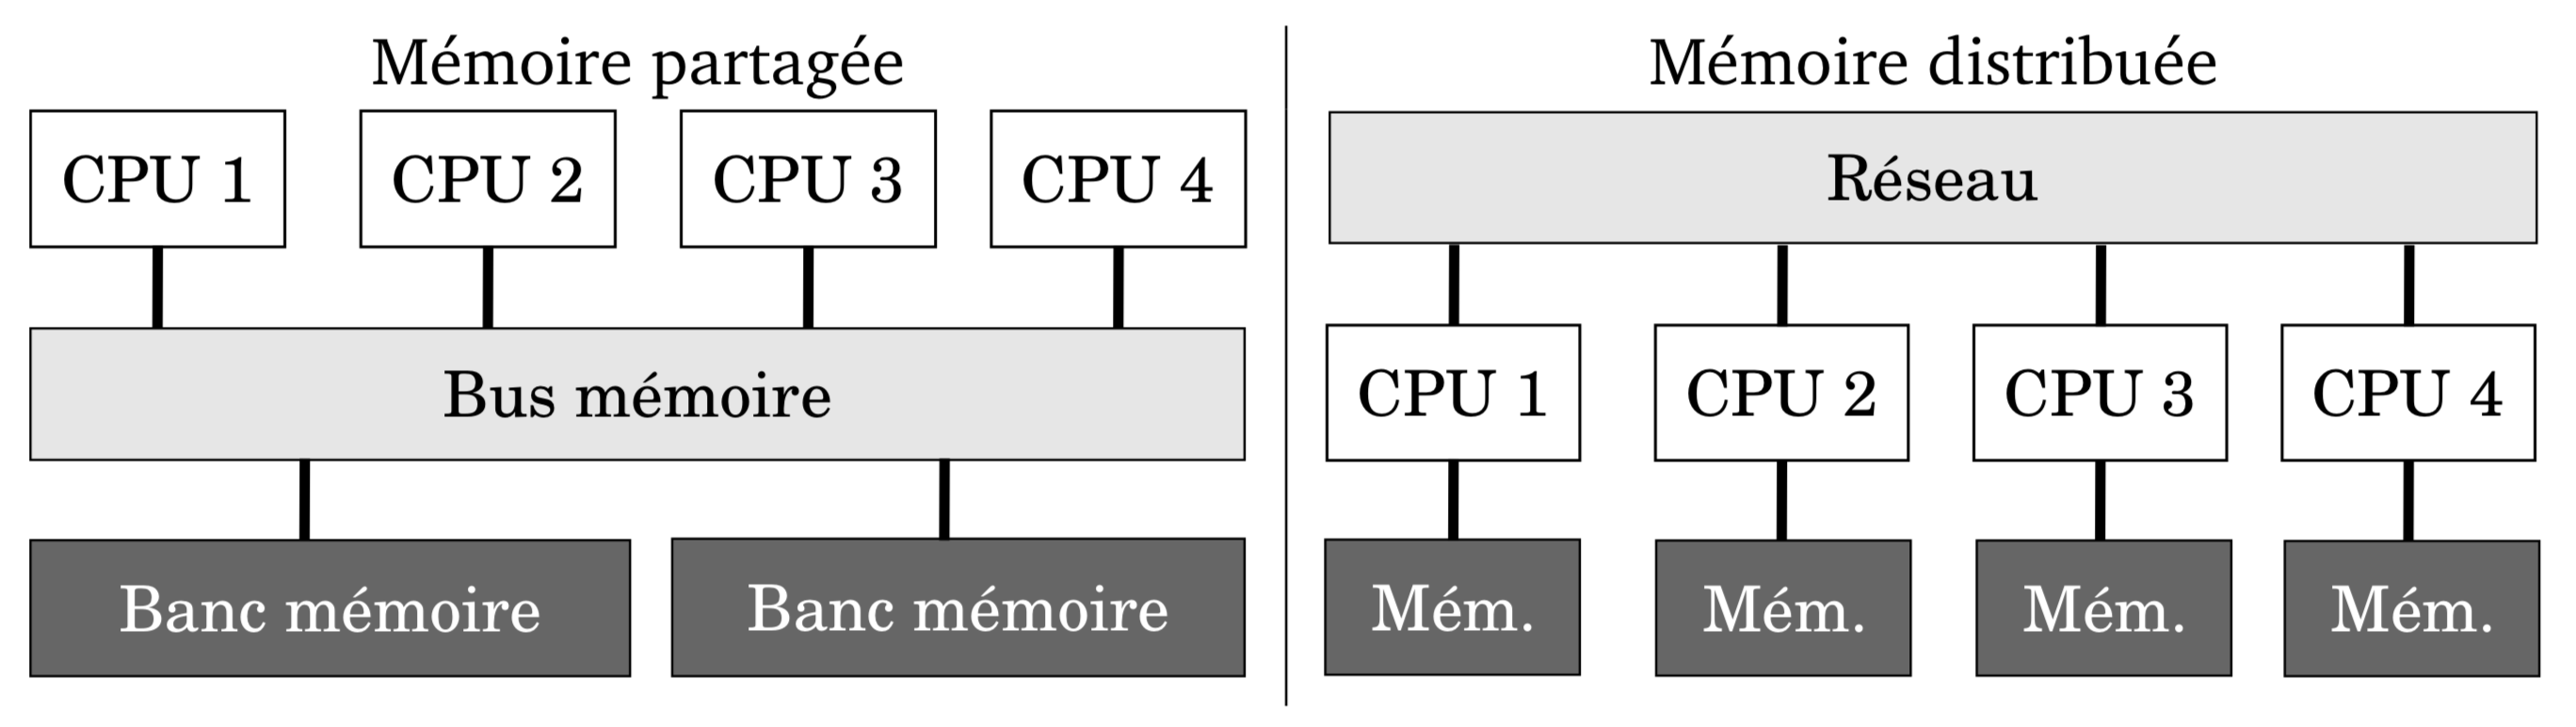
\includegraphics[width=14cm]{images/edl_ditribue_partage.png}
                \caption{\label{fig:edl_ditribue_partage} En fonction de l'architecture et du mode d'accès mémoire, deux paradigmes de programmations peuvent être utilisés (graphique extrait de \cite{Valat2016}).}
            \end{figure}
        
        
        
            
        \paragraph{Programmation à mémoire distribuée.}  
               
            Le paradigme de programmation à mémoire distribuée doit être utilisé lorsque les différents processus n'ont pas accès au même espace mémoire. Les communications entre les ressources de calculs sont alors réalisées par le système d'interconnexion. L'avantage de telles architectures est de permettre d'agréger plus ou moins de ressources en fonction du besoin d'un utilisateur. La performance de la solution est alors dépendante du nombre de serveurs utilisés et permet une plus grande flexibilité. 
            
            Les données nécessaires pour les calculs ainsi que les résultats temporaires doivent être explicitement transférés par l'utilisateur. Pour cela, les programmeurs peuvent utiliser des librairies de \textit{passage de messages}, dont le standard le plus utilisé est une \gls{mpi}. Le standard définit la sémantique des différentes fonctions, identifie les tâches distribuées et propose des moyens d'échange et de synchronisation entre les processus. Le standard est implémenté par des librairies telles que \verb|OpenMPI|, \verb|MPICH-2| ou encore \verb|IntelMPI|. Chaque noeud ayant son propre système d'exploitation, les librairies doivent être installées sur tous les serveurs utilisés. 
        
            La principale difficulté de ce paradigme de programmation est la nécessité de réaliser explicitement les mouvements de données entre les noeuds. L'exécution d'une application peut alors être résumée en 3 étapes. La \autoref{fig:scatter_gather} présente les étapes 1 et 3 d'un programme de calcul à mémoire distribuée:
            \begin{enumerate}
                \item La première étape consiste à répartir le jeu de données à l'aide d'opérations de type \textit{scatter} (voir \autoref{fig:scatter}). 
                \item La deuxième étape est la réalisation du calcul par chaque ressource. Cette étape utilise le paradigme de programmation à mémoire partagée (voir ci-dessous).
                \item Lorsque chacune d'entre elles a terminé son calcul, des opérations de type \textit{gather} (voir \autoref{fig:gather}) permettent de récolter l'ensemble des résultats partiels, pour calculer le résultat final.
            \end{enumerate}
            Les étapes 1 et 3 utilisent le système d'interconnexion du supercalculateur. La performance de celui-ci peut fortement impacter celle des applications. Cette particularité est à l'origine de nombreuses erreurs et rend la programmation à mémoire distribuée difficile. Le programmeur doit avoir à sa disposition des outils lui permettant de suivre l'évolution de chaque phase pour déceler des problèmes de synchronisation ou de déséquilibre de charge.
        
        
            \begin{figure}[t!]
                \centering
                \begin{subfigure}[t]{0.48\textwidth}
                    \centering
                    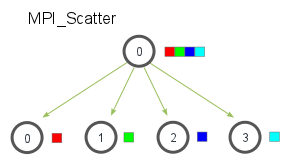
\includegraphics[width=.8\linewidth]{images/scatter.png}
                    \caption{\label{fig:scatter}Les opérations de \textit{scatter} permettent de répartir un jeu de données entre les ressources.}
                \end{subfigure}\hfill
            \begin{subfigure}[t]{0.48\textwidth}
                    \centering
                    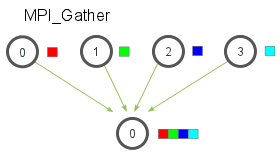
\includegraphics[width=.8\linewidth]{images/gather.png}
                    \caption{\label{fig:gather}Chaque ressource renvoie son résultat local pour calculer le résultat final du calcul.}
                \end{subfigure}
                \caption{\label{fig:scatter_gather}Les deux opérations principales de la programmation à mémoire distribuée sont de répartir (\textit{a}) et de récolter (\textit{b}) les données utilisées par les différentes ressources participant à la résolution\protect\footnotemark.}
            \end{figure}
            \footnotetext{Source des graphiques - \url{https://mpitutorial.com/tutorials/mpi-scatter-gather-and-allgather/}}
               
               
           
        %%%%%%%%%%%%%%%%%%%%%%%%%%%%%%%%%%%%%%%%%%%%%%
        \paragraph{Programmation à mémoire partagée.} \label{sec:prog_partagee}
            
            Lorsque toutes les ressources de calculs ont accès au même espace mémoire, il est conseillé d'utiliser le paradigme de programmation à mémoire partagée. Comme il n'est plus utile de transférer les données explicitement entre les ressources de calcul, il est possible d'utiliser des \gls{thread} (processus légers). Pour profiter des niveaux de parallélisme $2$ et $3$ (voir \autoref{fig:parallele_hpc}) les programmeurs peuvent avoir recours à des librairies ou même des langages spécifiques aux processeurs ciblés. Pour les processeurs, des librairies telles que \verb|OpenMP| ou \verb|Pthread| sont utilisées pour accéder au niveau $3$ de parallélisme qui consiste à répartir l'application sur les différents coeurs. Les accélérateurs de type GP-GPU peuvent être programmés à l'aide d'\verb|OpenCL| ou de \verb|CUDA|. Ces librairies sont basées sur le modèle de programmation \verb|fork/join| (voir \autoref{fig:openmp}). Lorsqu'une partie du code doit être exécutée en parallèle, le thread \textit{maître} se dédouble (\textit{fork}) en plusieurs threads pouvant être exécutés indépendamment sur différents coeurs. Une fois les tâches réalisées, les threads sont arrêtés et le programme continue son exécution séquentiellement. Ce modèle de programmation utilisant la même mémoire partagée, le programmeur doit veiller à ce que les différents threads utilisent des données en commun. Un avantage d'\verb|OpenMP| est sa facilité d'utilisation pour exprimer le parallélisme depuis le code source de l'application. À l'aide de directives préprocesseur, les zones exécutables en parallèle doivent être annotées à l'aide de \verb|#pragma|. Différentes options permettent de définir le nombre de threads à générer, la façon de partager le travail ou encore définir le mode d'accès aux données (partagé, privé). Le code listé dans l'\autoref{lst:openmp} permet de répartir les différentes itérations d'une boucle (indépendantes) entre les threads.
            
\begin{lstlisting}[language=C, caption=Distribution des itérations d'une boucle à l'aide d'OpenMP, label=lst:openmp]
#pragma omp parallel for
for (i=0;i<20;i++)
    a[i]=b[i] + 42;
\end{lstlisting}

                \begin{figure}
                \center
                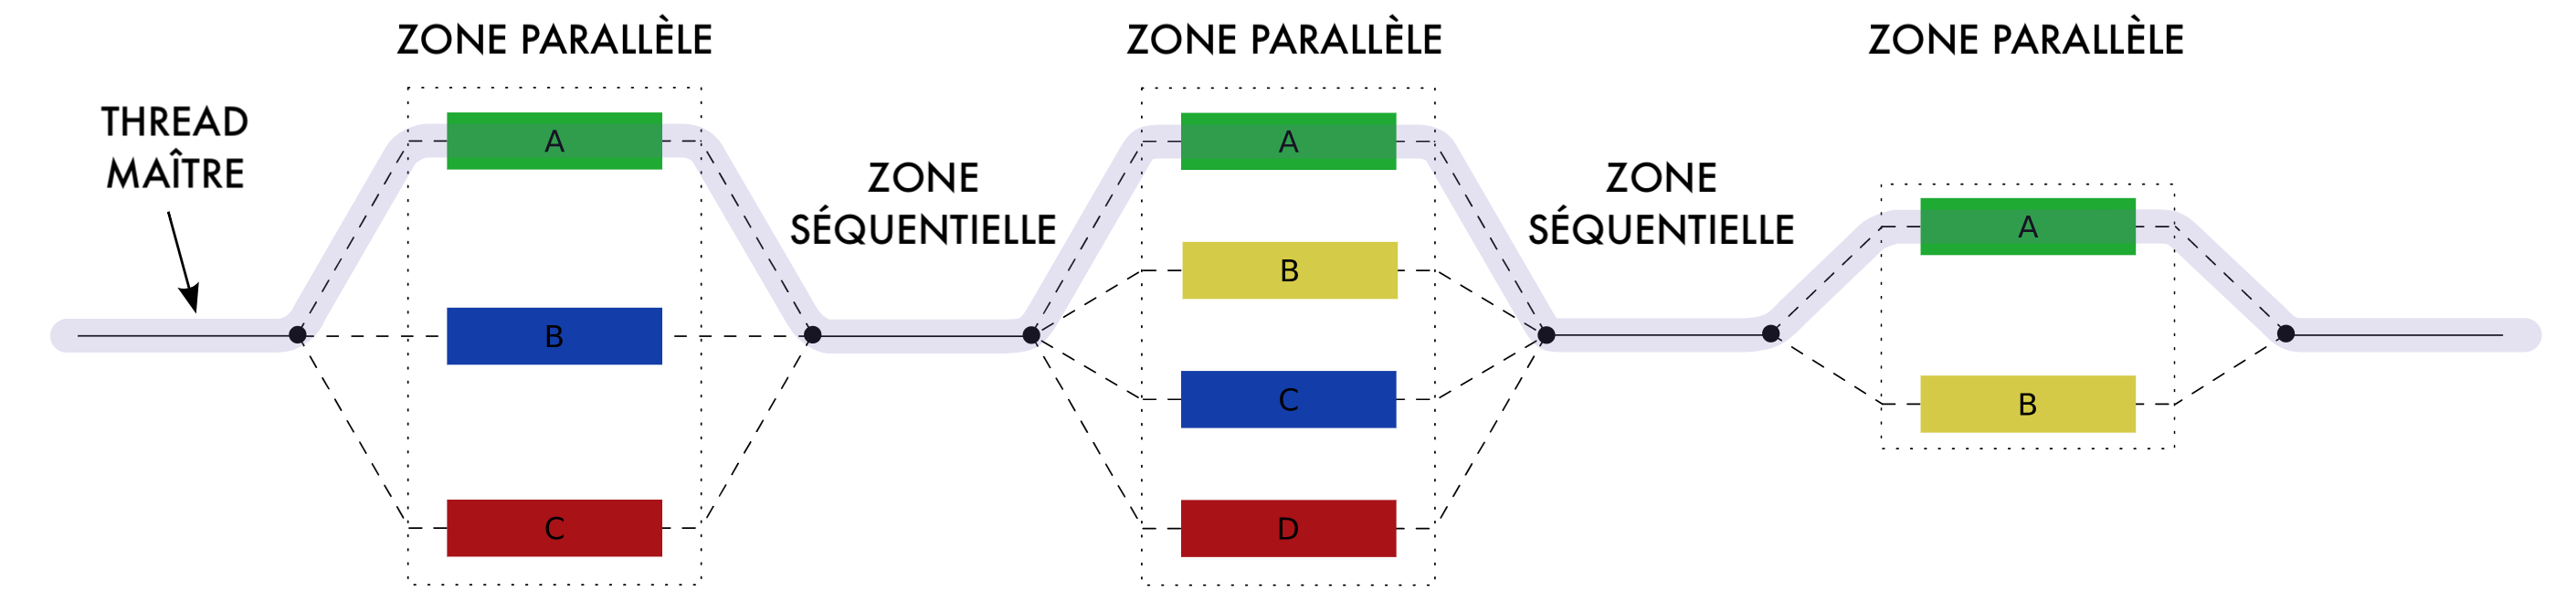
\includegraphics[width=14cm]{images/openmp.png}
                \caption{\label{fig:openmp} Pour accéder au parallélisme des coeurs, OpenMP crée des \textit{threads} indépendants\protect\footnotemark.}
                \end{figure}
                \footnotetext{Graphique adapté de \url{https://en.wikipedia.org/wiki/Fork\%E2\%80\%93join_model}}
                

\subsection{Performance de la parallélisation}
\label{sec:parallele_perf}
%%%%%%%%%%%%%%%%%%%%%%%%%%%%%%%%%%%%%%%%%%%%%%%%%%%%%%%%%%
    
        L'utilisation d'un supercalculateur a pour objectif d'accélérer l'exécution d'une application. Cette accélération peut alors permettre d'obtenir des résultats plus rapidement ou bien d'étudier des problèmes plus complexes. L'accélération d'une application, notée $Speedup(P)$, correspond au rapport entre le temps nécessaire pour exécuter l'application sur une ressource unique (noté $T_{sequentiel}$) et le temps nécessaire lorsque $P$ ressources identiques sont utilisées (noté $T_{parallele}$). L'accélération est dite optimale lorsque le temps de résolution $T_{parallele}(P)$ évolue linéairement avec le nombre $P$ de ressources. On parle alors d'accélération linéaire:
        
        \begin{equation}
        \label{eq_speedup}
        Speedup_{lineaire} (P) = \frac{T_{sequentiel}}{T_{parallele}(P)} = P
        \end{equation}
        
        Prenons l'exemple d'une application dont le temps nécessaire à l'exécution prend  $T_{sequentiel} = 2$ minutes. Une accélération linéaire avec l'utilisation de $P = 4$ processeurs pendrait alors $T_{parallele} = 30$ secondes. En pratique il est très rare d'obtenir une telle accélération, car certaines parties du code ne peuvent pas être parallélisées (transmission des données en programmation à mémoire distribuée, zone critique en programmation à mémoire partagée, synchronisation). 
        Pour évaluer la capacité d'une plateforme à utiliser efficacement les ressources supplémentaires pour l'exécution d'une application, il est courant de mesurer sa scalabilité. La scalabilité d'une application est un indicateur permettant d'évaluer sa capacité à \textit{passer à l'échelle}, c'est-à-dire d'évaluer l'accélération de son exécution lorsque des ressources de calculs supplémentaires sont allouées. On distingue alors deux scalabilités: la forte et la faible (voir \autoref{fig:scaling}). Les résultats des tests de scalabilité forte et faible permettent de choisir un nombre adapté de ressources à utiliser pour une application.
        
            \begin{figure}[t!]
                \centering
                \begin{subfigure}[t]{0.48\textwidth}
                    \centering
                    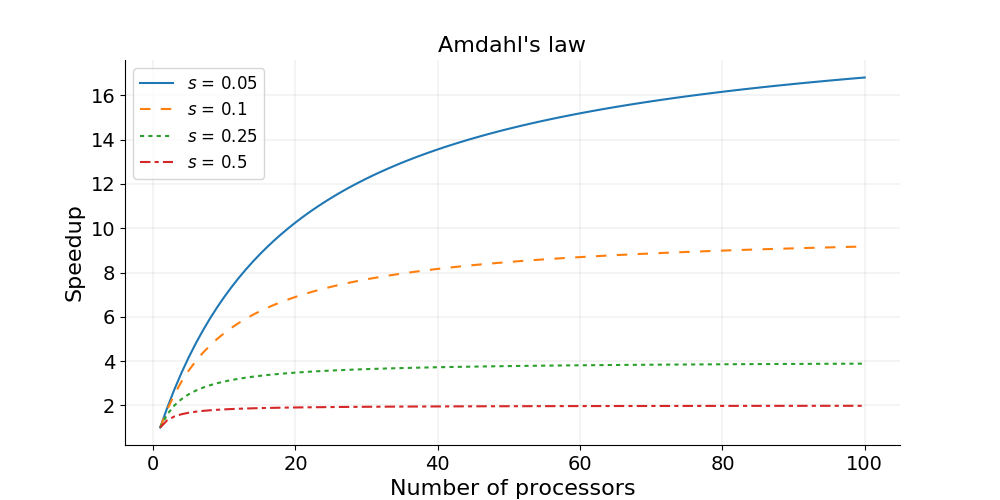
\includegraphics[width=1.05\linewidth]{images/scaling_amdahl.png}
                    \caption{\label{fig:scaling_amdahl}Loi d'Amdahl: la scalabilité forte utilise un problème de complexité constante.}
                \end{subfigure}\hfill
            \begin{subfigure}[t]{0.48\textwidth}
                    \centering
                    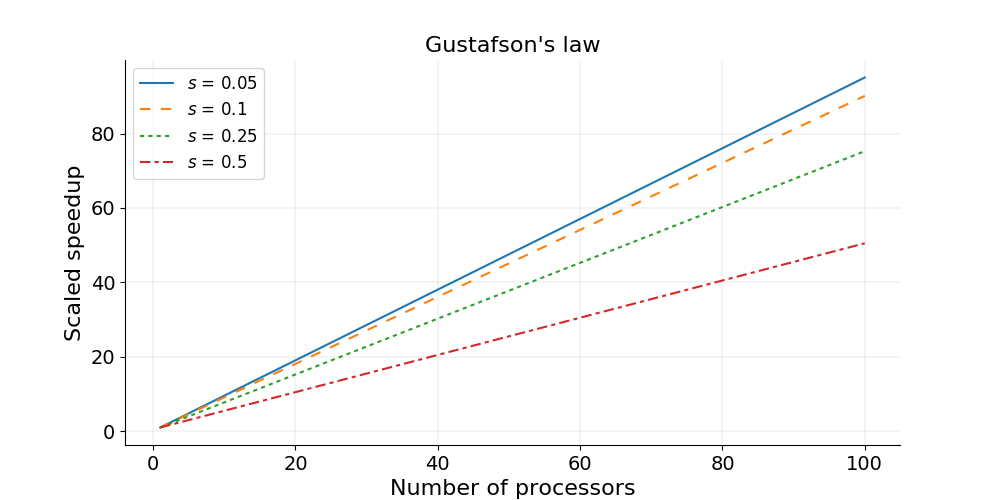
\includegraphics[width=1.05\linewidth]{images/scaling_gustafson.png}
                    \caption{\label{fig:scaling_gustafson}Loi de Gustafson: la scalabilité faible utilise un problème de complexité croissante.}
                \end{subfigure}
                \caption{\label{fig:scaling} Évolution de la scalabilité forte et faible lorsque $P$ processeurs sont utilisés pour l'exécution d'une application ayant une proportion $s$ de code séquentiel\protect\footnotemark.}
            \end{figure}
            \footnotetext{Source des graphiques - \url{https://www.kth.se/blogs/pdc/2018/11/scalability-strong-and-weak-scaling}}
            

    \subsubsection{Scalabilité forte} \label{sec:amdhal}
    %%%%%%%%%%%%%%%%%%%%%%%%%%%%%%%%%%
        
        En 1967, l'ingénieur Gene Amdahl a étudié et théorisé l'évolution de l'accélération d'une application avec l'ajout de ressources de calculs, créant ainsi la loi éponyme \cite{Amdahl1967}. La taille du problème étant fixe, chaque unité de calcul a donc moins de travail à réaliser. Idéalement, le temps d'exécution doit être réduit d'un facteur $1/P$ lorsque $P$ ressources sont ajoutées (voir \autoref{fig:scaling_amdahl}). Une application de calcul parallèle n'étant jamais totalement parallélisable, elle possède toujours une proportion de code devant être exécuté séquentiellement. Cette proportion est notée $s$. L'ajout de ressources de calcul n'est alors bénéfique que pour la proportion de code dit parallélisable et noté $1-s$. Le temps nécessaire pour l'exécution de l'application est la somme du temps passé dans la zone séquentielle et de celui passé dans la zone parallèle. En utilisant $P$ processeurs le temps de l'exécution parallèle peut être calculé ainsi: 

        
            \begin{equation}
            T_{parallele}(P) = s \times T_{sequentiel} + \frac{(1-s) \times T_{sequentiel}}{P}
            \end{equation}
        
        L'accélération de l'application peut alors être calculée grâce à l'\autoref{eq_speedup} donnant lieu à l'équation suivante, appelée loi d'Amdahl:
        
                
            \begin{equation}
            \label{eq_amdahl}
            Speedup (P) = \frac{T_{sequentiel}}{s \times T_{sequentiel} + \frac{(1-s) \times T_{sequentiel}}{P}} =  \frac{1}{s + \frac{1-s}{P}}
            \end{equation}
        
        L'accélération d'une application dépend donc du nombre de ressources de calculs supplémentaires allouées à la résolution de l'application, mais aussi de la proportion de zones exécutables en parallèle. La \autoref{fig:scaling_amdahl} montre l'importance de l'influence de la proportion de code séquentiel $s$ sur l'accélération de l'application. Grâce à la loi d'Amdahl, il est possible de donner la limite théorique de l'accélération $Speedup$ d'une application (notée $Speedup_{max}$),  lorsque des ressources de calculs supplémentaires sont utilisées pour la résolution d'un problème de taille fixe. L'accélération maximale d'une application utilisant 95\% de son temps d'exécution dans une fonction entièrement parallélisable peut être calculée par la limite suivante:         
        \begin{equation}
        Speedup_{max} =  \lim_{p\to\infty}    \frac{1}{0.05 + \frac{0.95}{P}} = \frac{1}{0.05} = 20         
        \end{equation}
        Quel que soit le nombre de ressources allouées à l'exécution de cette application, l'application étudiée en exemple ne pourra jamais être accélérée de plus de 20 fois.  
        
        
        %Les coûts engendrés par ces différentes opérations sont notés $T_{couts}$. La durée de l'exécution du programme parallèle peut alors être calculée par la formule suivante:
                %En supposant des coûts $T_{couts}$ associés à l'utilisation du parallélisme, le temps d'exécution du programme parallélisé peut être calculé ainsi:
        %\begin{equation}
        %T_{parallele} = \frac{T_{sequentiel}}{P} + T_{couts}
        %\end{equation}
        
       
    \subsubsection{Scalabilité faible} 
    %%%%%%%%%%%%%%%%%%%%%%%%%%%%%%%%%%
        
        La loi d'Amdahl est très utile pour montrer la nécessité de développer des applications avec la plus grande portion de code parallélisable. Cependant, la loi suppose une taille de problème constante. Lorsque des ressources de calculs supplémentaires sont disponibles, les applications utilisent généralement des jeux de données plus grands pour profiter de l'espace mémoire supplémentaire. La loi d'Amdahl supposant un jeu de donnée fixe n'est alors pas adaptée. Pour y remédier, Gustafson énonça une nouvelle loi en 1988 \cite{Gustafson1988} permettant de prendre cet aspect en considération. 
        Lorsque la taille du jeu de données augmente, la partie séquentielle du programme représente généralement une plus faible portion, car les données sont traitées dans les zones parallèles. Pour une application ayant une proportion de $1-s$ pouvant être exécutée en parallèle sur $P$ processeur, l'accélération peut être calculée par la loi de Gustafson:         
        \begin{equation}
            Speedup (P) = s + (1-s) * P         
        \end{equation}
        
        La scalabilité faible utilise une taille de problème qui évolue à mesure que des ressources supplémentaires sont allouées. Dans ce cas-là, la taille du problème pour chaque unité de calcul est fixe. Dans l'idéal, le temps d'exécution de l'application doit rester constant lors de l'ajout de ressources de calculs (voir \autoref{fig:scaling_gustafson}). Contrairement à la scalabilité forte, l'accélération obtenue par la scalabilité forte n'a pas de limite théorique. 
        
        
\section{Évolution de la performance des supercalculateurs}\label{sec:edl_evolution}
%%%%%%%%%%%%%%%%%%%%%%%%%%%%%%%%%%%%%%%%%%%%%%%%%%%%%%%%%%%

La performance des supercalculateurs a beaucoup évolué depuis leur apparition. Pour comprendre les défis que l'industrie doit relever pour poursuivre ces améliorations, nous nous sommes intéressés à l'évolution des performances de ces architectures ces 20 dernières années.


\subsection{Comparer la performance des supercalculateurs}
%%%%%%%%%%%%%%%%%%%%%%%%%%%%%%%%%%%%%%%%%%%%%

    Pour mesurer et comparer la performance des supercalculateurs, il est nécessaire d'avoir une application de référence. L'étalonnage (\textit{benchmarking}) est une pratique courante qui consiste à évaluer plusieurs solutions en leur faisant passer une épreuve commune. Dans le domaine informatique, cela permet de tester différentes architectures matérielles et d'évaluer leurs performances. Un des benchmarks les plus utilisés dans le domaine du HPC est celui développé par Jack Dongara en 1988: le benchmark HPL (High-Performance Linpack) \cite{Dongarra2003}. Ce benchmark est un code simple qui résout un système d'équations linéaires $Ax = B$, $A$ et $B$ étant deux matrices. Les performances évoluent linéairement avec le nombre de machines utilisées, car très peu de communications sont nécessaires. Le résultat est un nombre d'\gls{FLOPS} que la machine peut exécuter, ce qui rend la comparaison entre supercalculateurs aisée.
    Ce code permet de publier deux classements bisannuels: le Top500 et le Green500 (\autoref{fig:Top500}).

        \begin{figure}[b!]
                \centering
                \begin{subfigure}[t]{0.48\textwidth}
                    \centering
                    
\includegraphics[width=.4\linewidth]{images/Top500_logo.png}
                    \caption{\label{fig:Top500_logo}Top500}
                \end{subfigure}\hfill
            \begin{subfigure}[t]{0.48\textwidth}
                    \centering
                    
\includegraphics[width=.25\linewidth]{images/Green500_logo.png}
                    \caption{\label{fig:Green500_logo}Green500}
            \end{subfigure}
            \caption{\label{fig:Top500} Les classements du Top500 et du Green500 sont présentés deux fois par an lors de la conférence Supercomputing\protect\footnotemark}
        \end{figure}
        \footnotetext{\url{supercomputing.org/}}
        
    \subsubsection{Le Top500}\label{sec:Top500}
    %%%%%%%%%%%%%%%%%%%%%%%%%%%%%%%%%%%%%%%%%%%%%
        
        Le TOP500\footnote{\url{www.top500.org}} est un classement mondial qui classe, tous les 6 mois depuis 1993, les 500 supercalculateurs les plus puissants au monde. Ce classement se base sur le nombre maximum d'opérations flottantes qui peuvent être exécutées en une seconde (\gls{FLOPS}) lors de l'exécution du benchmark HPL. Cette unité a été choisie, car la grande majorité des codes utilisés dans les domaines précédemment cités exécutent des opérations sur des nombres flottants. Il s'avère donc judicieux de choisir ce dénominateur commun pour comparer les différentes architectures.

        Il faut cependant savoir que ce classement ne contient pas toutes les machines. En effet, certains industriels ne préfèrent pas apparaître dans ce classement. Stratégiquement parlant, il peut être intéressant de ne pas publier sa puissance de calcul et nous savons que certaines des infrastructures les plus puissantes n'y figurent pas. Cependant, ce classement permet d'apprécier les tendances que suivent la majorité des architectures.
        
        Au moment de l'écriture de ce manuscrit, le dernier classement disponible est celui de novembre 2019\footnote{Top500 novembre 2019 -  \url{www.top500.org/lists/2019/11/}}. Les principales caractéristiques des quatre premiers supercalculateurs sont présentées dans le \autoref{tab:top500}. Les États-Unis et la Chine possèdent chacun deux entrées et se partagent 70\% des performances totales du Top500 (32.3\% pour la Chine, 37.1\% pour les États-Unis). Concernant le système d'interconnexion, 6 des 10 premières entrées, ainsi que 141 des 500 supercalculateurs,  utilisent la technologie Infiniband.
        L'efficacité des supercalculateurs représente la capacité d'une plateforme à atteindre la performance théorique \verb|Rpeak|. Sur les 500 plateformes répertoriées, 100 d'entre elles ne parviennent pas à atteindre plus de 50\% de la performance théorique. Cette information est importante pour comprendre la difficulté qu'ont les applications à utiliser ces plateformes efficacement. Le benchmark \verb|HPL| est un code très simple, avec peu d'accès mémoire. Les applications réelles, plus complexes, ont beaucoup de mal à atteindre la performance théorique. Depuis quelques années, le classement du Top500 donne la performance d'un second benchmark (HPCG, voir \autoref{sec:hpcg}). Pour ce benchmark, plus fidèle aux comportements d'applications réelles, aucune des plateformes n'atteint une efficacité supérieure à 4\%. Pour avoir une meilleure vision de l'efficacité des plateformes, le classement du Green500 peut être consulté.


        \begin{table}[]
\centering
\resizebox{\textwidth}{!}{%
\begin{tabular}{|c|c|c|r|r|r|c|r|r|r|}
\hline
\rowcolor[HTML]{EFEFEF} 
\textbf{Pos.} & \textbf{Nom} & \multicolumn{1}{l|}{\cellcolor[HTML]{EFEFEF}\textbf{Country}} & \multicolumn{1}{l|}{\cellcolor[HTML]{EFEFEF}\textbf{Nb. coeurs}} & \multicolumn{1}{l|}{\cellcolor[HTML]{EFEFEF}\textbf{Coeurs accélérateur}} & \multicolumn{1}{l|}{\cellcolor[HTML]{EFEFEF}\textbf{Alimentation (MW)}} & \multicolumn{1}{l|}{\cellcolor[HTML]{EFEFEF}\textbf{Accélérateur}} & \multicolumn{1}{c|}{\cellcolor[HTML]{EFEFEF}\textbf{Rpeak}} & \multicolumn{1}{c|}{\cellcolor[HTML]{EFEFEF}\textbf{Rmax}} & \multicolumn{1}{c|}{\cellcolor[HTML]{EFEFEF}\textbf{Éfficacité}} \\ \hline
1 & Summit & United States & 2414592 & 2211840 & 10 & NVIDIA GPU & 200 & 148 & 0.74 \\ \hline
2 & Sierra & United States & 1572480 & 1382400 & 7 & NVIDIA GPU & 125 & 94 & 0.75 \\ \hline
3 & Sunway TaihuLight & China & 10649600 & 0 & 15 & None & 125 & 93 & 0.74 \\ \hline
4 & Tianhe-2A & China & 4981760 & 4554752 & 18 & Matrix-2000 & 100 & 61 & 0.61 \\ \hline
\end{tabular}%
}
\caption{Classement du Top500 de novembre 2019. Les puissances Rpeak (puissance théorique) et Rmax (puissance mesurée par HPL) sont données en pétaFLOPS ($10^{15}$ FLOPS). L'efficacité est le rapport entre Rmax et Rpeak.}
\label{tab:top500}
\end{table}
   
    \subsubsection{Le Green500}
    %%%%%%%%%%%%%%%%%%%%%%%%%%%%%
        
        Un second classement a vu le jour en 2007 appelé le Green500\footnote{Green500 - \url{www.top500.org/green500/}}. Il classe les supercalculateurs selon un critère d'efficacité énergétique. Cette efficacité mesure le nombre d'opérations sur un nombre flottant réalisé pour 1 watt d'énergie fourni au supercalculateur. 
    
        En effet, ces vingt dernières années, les évolutions technologiques et l'augmentation de la taille des supercalculateurs n'avaient pas de limite physique. Cette course à la performance n'était dictée que par les budgets disponibles pour leur construction. Ainsi, l'émergence de plateformes consommant de grandes quantités d'énergie et très peu efficace a été constatée (voir le classement du Top500). 
        
        En novembre 2019\footnote{\url{www.top500.org/green500/lists/2019/11/}}, les 34 premiers supercalculateurs utilisent tous des accélérateurs. La majorité étant des GPU Nvidia Tesla. Il est intéressant de noter que la deuxième place du classement est tenue par une plateforme basée sur le processeur PEZY-SC2 conçu par l'entreprise PEZY et fabriqué par TSMC. Seul le premier du classement n'utilise pas d'accélérateurs (voir \autoref{tab:green500}). Il utilise un processeur ARM basse fréquence pouvant exécuter des instructions vectorielles SVE (Scalable Vector Extensions) sur 512 bits.

        
        \begin{table}[]
            \centering
            \resizebox{0.80\textwidth}{!}{%
            \begin{tabular}{|c|r|l|l|r|r|r|r|}
            \hline
            \rowcolor[HTML]{EFEFEF} 
            \textbf{Position} & \multicolumn{1}{c|}{\cellcolor[HTML]{EFEFEF}\textbf{TOP500}} & \multicolumn{1}{c|}{\cellcolor[HTML]{EFEFEF}\textbf{Processeur}} & \multicolumn{1}{c|}{\cellcolor[HTML]{EFEFEF}\textbf{Accélérateur}} & \multicolumn{1}{c|}{\cellcolor[HTML]{EFEFEF}\textbf{Rmax}} & \multicolumn{1}{c|}{\cellcolor[HTML]{EFEFEF}\textbf{Rpeak}} & \multicolumn{1}{c|}{\cellcolor[HTML]{EFEFEF}\textbf{Efficacité}} & \multicolumn{1}{c|}{\cellcolor[HTML]{EFEFEF}\textbf{Efficacité énergétique}} \\ \hline
            1 & 159 & Fujitsu A64FX & Aucun & 1.99 & 2.35 & 0.84 & 16.876 \\ \hline
            2 & 420 & Xeon D-1571 & PEZY-SC2 700Mhz & 1.30 & 1.79 & 0.72 & 16.256 \\ \hline
            3 & 24 & IBM POWER9 & Volta GV100 & 8.04 & 11.12 & 0.72 & 15.771 \\ \hline
            4 & 373 & IBM POWER9 & Tesla V100 SXM2 & 1.46 & 1.73 & 0.84 & 15.574 \\ \hline
            \end{tabular}%
            }
            \caption{Classement du Green500 de novembre 2019 selon l'efficacité énergétique (en gigaFLOPS/Watts). Les puissances Rpeak (puissance théorique) et Rmax (puissance mesurée par HPL) sont données en pétaFLOPS ($10^{15}$ FLOPS).}
            \label{tab:green500}
        \end{table}
        
        
\subsection{Évolution des performances des supercalculateurs}
%%%%%%%%%%%%%%%%%%%%%%%%%%%%%%%%%%%%%%

    Le classement du Top500 a de nombreux avantages, dont celui de promouvoir le HPC au grand public. Cependant, un effet de bord de ce classement est de motiver les constructeurs pour développer des architectures ayant de bonnes performances lors de l'exécution du benchmark HPL. Or, ce code n'est pas représentatif des applications réelles et nous pouvons nous demander si son utilisation pour l'établissement du Top500 n'a pas été contre-productive. Bien que certains des supercalculateurs les plus puissants n'y figurent pas, l'évolution du Top500 permet d'obtenir un aperçu des évolutions de performances des architectures.
    
    Pour avoir une vision globale de son évolution, nous étudions la performance cumulée des 500 supercalculateurs depuis le premier classement (voir \autoref{pic_top500perf_evo}). Nous distinguons deux phases: avant et après 2012. 
    Les performances du Top500 ont évolué d'un facteur 1000 tous les 11 ans, conformément aux performances prédites par la loi de Moore. À partir de 2013, il faut attendre en moyenne 20 ans pour voir la performance des supercalculateurs augmenter dans la même proportion.
    Dans cette section, nous discutons des différents facteurs qui ont permis l'évolution constante des performances des architectures pendant près de 20 ans et étudions les freins qui empêchent de poursuivre ce rythme. La majorité des améliorations évoquées sont présentées dans l'\aref{chap:sota:materiel}.

    
    \begin{figure}
        \center
        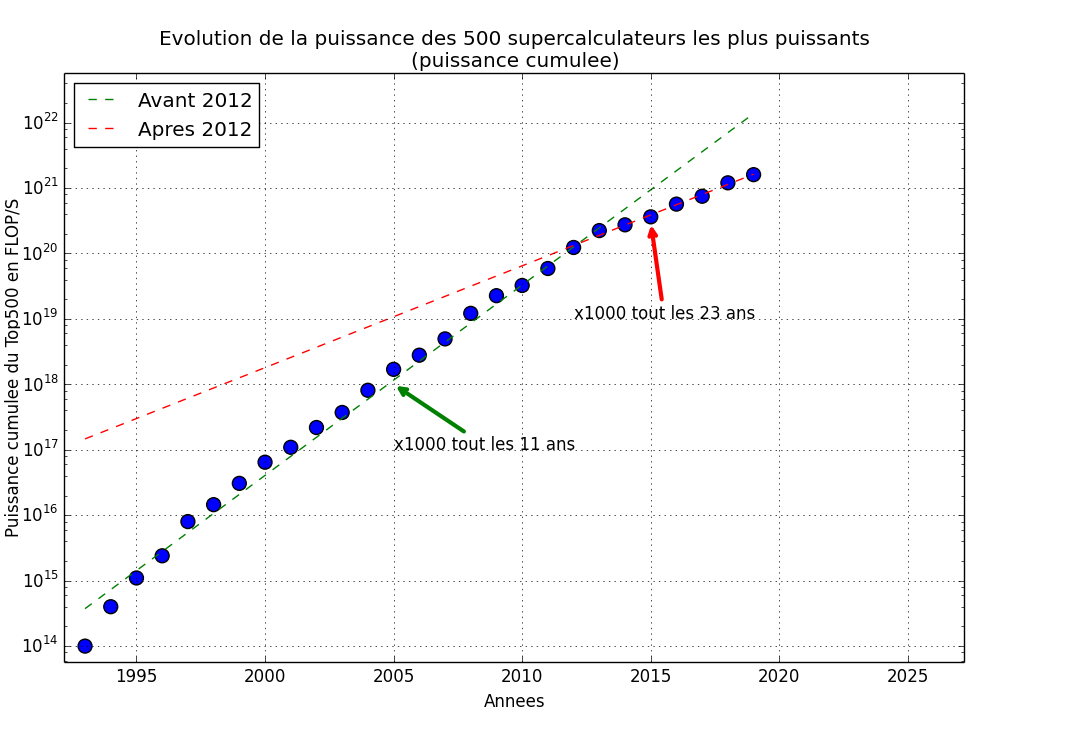
\includegraphics[width=12cm]{images/top500_evolution.png}
        \caption{\label{pic_top500perf_evo} Évolution de la performance cumulée des 500 supercalculateurs les plus puissants au monde. La pente de l'évolution diminue à partir de 2012.}
    \end{figure}


    \subsubsection{Avant 2012}\label{sec:proc_evo_2012}
    %%%%%%%%%%%%%%%%%%%%%%%%%%%%
    
        Les supercalculateurs ont pu bénéficier de nouvelles technologiques ainsi que de nombreuses innovations techniques.
        
        \begin{figure}[t!]
            \centering
            \begin{subfigure}[t]{0.33\textwidth}
                \centering
                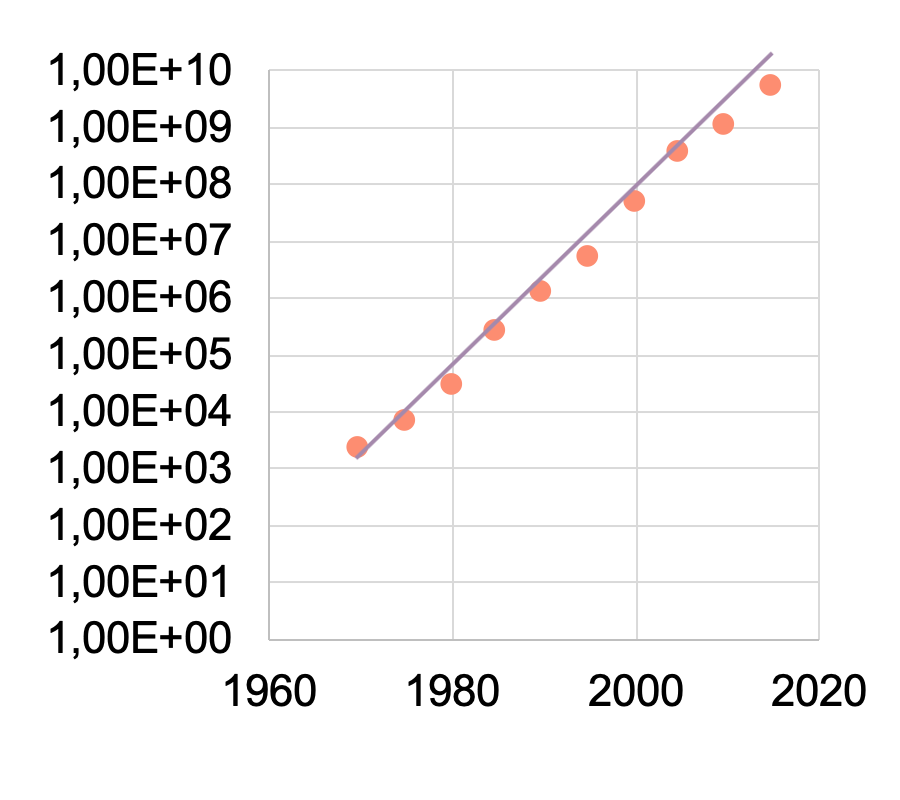
\includegraphics[width=\linewidth]{images/evo_transistor.png}
                \caption{\label{fig:evo_transistor}Évolution du nombre de transistors (\autoref{sec:denard})}
            \end{subfigure}\hfill
            \begin{subfigure}[t]{0.33\textwidth}
                \centering
                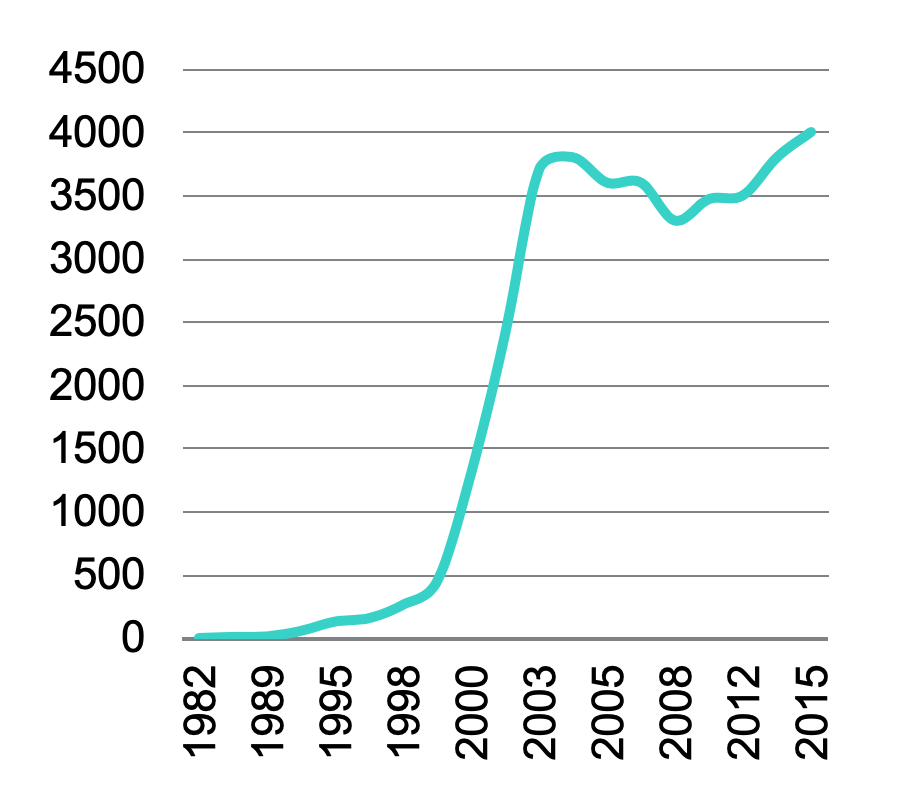
\includegraphics[width=\linewidth]{images/evo_freq.png}
                \caption{\label{fig:evo_freq}Évolution de la fréquence (\autoref{sec:frequency})}
            \end{subfigure}\hfill
            \begin{subfigure}[t]{0.33\textwidth}
                    \centering
                    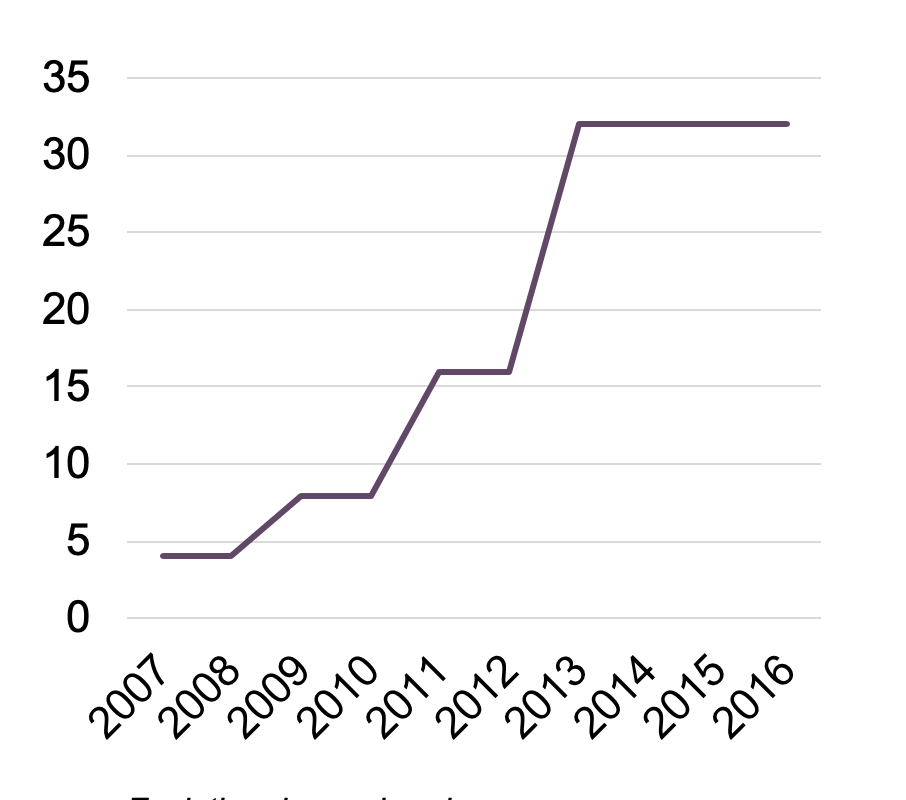
\includegraphics[width=\linewidth]{images/evo_core.png}
                    \caption{\label{fig:evo_core}Évolution du nombre de coeurs (\autoref{sec:multicore})}
            \end{subfigure}
            \caption{\label{fig:evo_proc}Évolutions technologiques principales des processeurs. Ces différentes évolutions sont présentées dans l'\autoref{annexe:CHAPITRE_ARCHITECTURE}.}
        \end{figure}
        
            \paragraph{Les processeurs.} Dans l'\aref{chap:sota:materiel}, nous présentons les différentes évolutions technologiques dont ont pu bénéficier les processeurs. La \autoref{fig:evo_proc} résume les trois principales évolutions.
            Grâce à l'affinement des procédés de gravure, le nombre de transistors a évolué exponentiellement (voir \autoref{fig:evo_transistor}).  
            En miniaturisant les transistors et en utilisant des systèmes de refroidissement plus efficaces, la fréquence des processeurs a pu être augmentée de plusieurs facteurs (voir \autoref{fig:evo_freq}).
            Lorsque la fréquence n'a plus pu être augmentée, les architectures parallèles ont été développées, donnant naissance aux processeurs multicoeurs (voir \autoref{fig:evo_core}). La microarchitecture elle-même a reçu de nombreuses améliorations: l'utilisation de pipeline (voir \autoref{sec:pipeline}) pouvant être superscalaire (voir \autoref{sec:superscalar}), ainsi que le développement d'unités de calculs pouvant exécuter des instructions vectorielles (voir \autoref{sec:cpu_vectoriel}).
            
            \paragraph{Les mémoires.} La performance des processeurs évoluant, celle des mémoires a aussi dû être amélioré pour fournir les données nécessaires aux traitements plus rapidement. Les principales améliorations sont dues à l'utilisation de nouvelles technologies mémoires (voir \autoref{sec:memory}), l'augmentation du nombre de canaux reliant la mémoire au processeur ou encore l'implémentation d'une hiérarchie de mémoire (voir \autoref{sec:hierarchie_true}). Celle-ci permettant aux applications de profiter du principe de localité (voir \autoref{sec:locality}).
            
        
    \subsubsection{Après 2012}
    %%%%%%%%%%%%%%%%%%%%%%%%%%%%
    
        En étudiant l'évolution de la puissance des supercalculateurs (voir \autoref{pic_top500perf_evo}), nous remarquons un ralentissement à partir des années 2010-2012. Ce ralentissement n'est pas dû à un seul facteur, mais à un ensemble de contraintes. En effet, les leviers et évolutions technologiques qui permettaient de tenir cette cadence ne sont plus disponibles aujourd'hui ou sont en fin de course (voir \autoref{fig:evo_proc}). Si certaines lois ont assuré une évolution continue de la performance des processeurs pendant plusieurs dizaines d'années, une partie du ralentissement de l'évolution des performances du Top500 peut être expliquée par leur \textit{essoufflement} \cite{FrancoisBodin2015}.

       
        \begin{figure}
            \center
            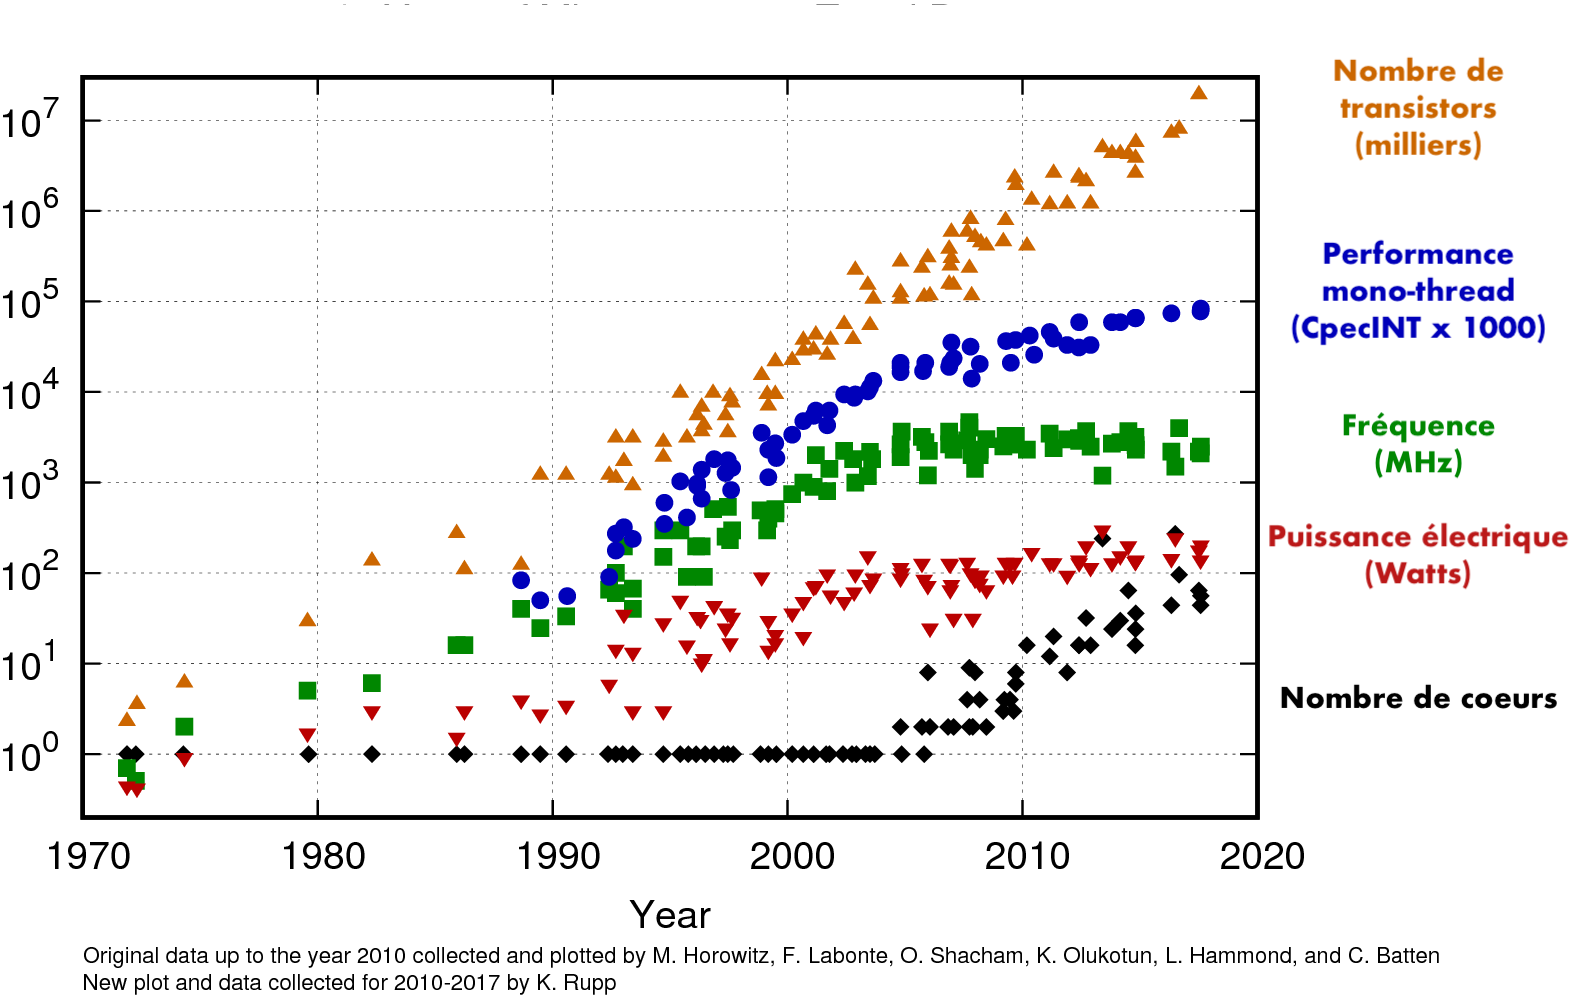
\includegraphics[width=12cm]{images/evo_proc.png}
            \caption{\label{fig:evo_proc} Évolution des principales caractéristiques des processeurs (données originales tirées de \cite{rupp40years}\protect\footnotemark).}
        \end{figure}
        \footnotetext{Les données sont accessibles sur le dépôt GitHub de l'auteur:  \url{https://github.com/karlrupp/microprocessor-trend-data}}
        
%%%%%%%%%%%%%%%%%%%%%%%%%%%%%%%%%%%%%%%%%%%%%%%%%%%%%%%%%%%%%%%%%%%%%%%%%%%% 
      
        \paragraph{Fin de validité de la loi de Moore.}\label{sec:end_mooore} 
            
            La loi de Moore \cite{Moore1998} prévoyait que les architectures pourraient doubler leur nombre de transistors, tous les deux ans \cite{Moore75}, à coût constant (voir \autoref{sec:moore}). Malheureusement, les fondeurs ne parviennent plus à suivre le rythme dicté par la loi énoncée par Gordon Moore, pour des raisons principalement techniques (gravure), de coût \cite{Brooks2017} et de limite physique. La miniaturisation continue des transistors, dont la taille actuelle est de quelques nanomètres, rend la circulation des courants électriques instable. La bonne circulation des signaux électriques dans les circuits ne pouvant plus être garantie, il n'est alors plus possible de réduire leur taille.
            À partir de 2013, l'évolution des performances du Top500 passe pour la première fois sous les performances prévues par la loi de Moore (\autoref{fig:moore_vs_top500}).
            

            \begin{figure}
            \center
            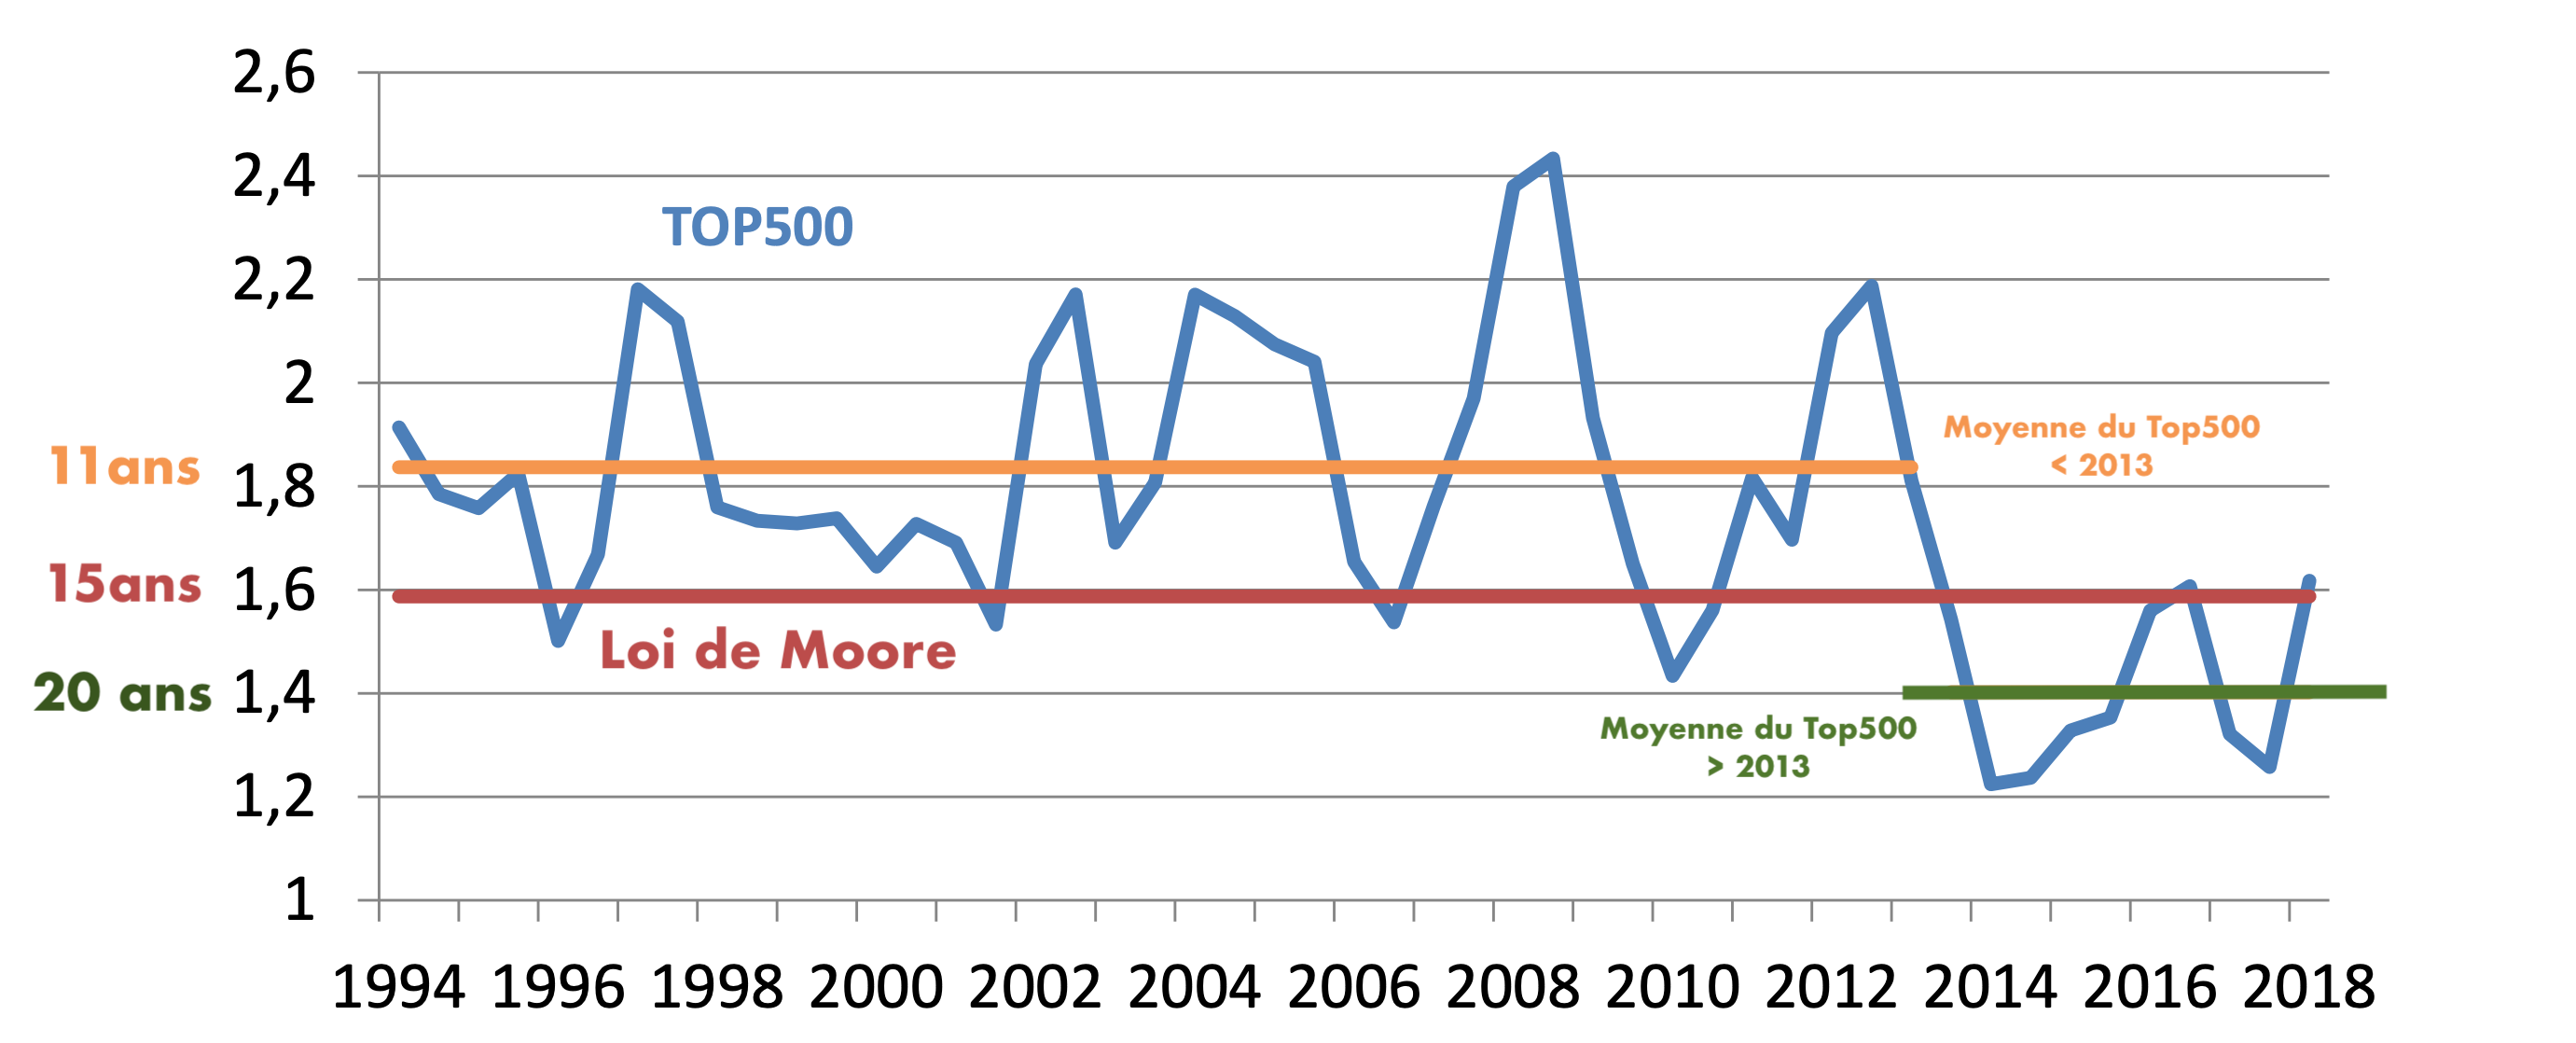
\includegraphics[width=16cm]{images/moore_vs_top500.png}
            \caption{\label{fig:moore_vs_top500}
             Facteur d'évolution annuelle des performances du Top500\protect\footnotemark. Jusqu'à 2013 la performance moyenne du Top500 évoluait d'un facteur 1.8, supérieur à l'évolution prédite par la loi de Moore (facteur 1.6). }
                \end{figure}
            \footnotetext{Graphique inspire de la présentation du Top500 lors de la conférence ISC18 - \textit{Highlights of the 51st TOP500 List}}

        \paragraph{Fin de la validé de la loi de Dennard.} 
                
            Dans l'\aref{sec:denard}, nous avons discuté de l'augmentation de la fréquence des processeurs et introduit \textbf{la loi de Dennard} \cite{Dennard1974}. Ces équations ont assuré l'augmentation de la fréquence des processeurs, de 40\% tous les 2 ans pendant plus de trente ans. À cause des courants de fuite \cite{Wulf1995} augmentant exponentiellement avec la finesse de gravure des transistors, la consommation électrique des processeurs a elle aussi augmenté. Dans la \autoref{sec:denard}, nous expliquons comment la réduction de la taille des transistors et l'augmentation de la fréquence des processeurs augmentent la consommation électrique de circuit. L'énergie utilisée par le processeur étant dissipée sous forme de chaleur, il est devenu très difficile de refroidir ces architectures. De plus, l'énergie nécessaire pour le refroidissement a un impact sur la consommation. Cette limitation physique empêchant d'augmenter la puissance électrique des processeurs est appelée \textit{power wall} \cite{Kuroda2001}.

        \paragraph{Budget.} 
            
            Le prix des supercalculateurs est un frein à la construction de centres toujours plus puissants. Les calculateurs les moins puissants du classement sont généralement ceux dont le budget est le faible. Grâce à l'analyse du Top500, nous pouvons estimer que l'économie est un des freins participant au ralentissement de l'évolution des performances des architectures (voir \autoref{fig:Top500_Poor}). Le décrochage des performances du Top500, autour de 2012, étudié dans la section précédente intervient plus de 4 ans après le décrochage du dernier du classement (en 2008). De plus, on peut étudier la répartition de la performance du Top500 entre les supercalculateurs. En 2004, il fallait agréger les 80 premiers supercalculateurs du classement pour obtenir la moitié de la performance cumulée du Top500. En 2019, il faut seulement cumuler la puissance des 28 premiers. Ceci montre que les plateformes en haut du classement ont tendance à augmenter leur performance plus vite que celles du bas.
            
            
    
            \begin{figure}
            \center
            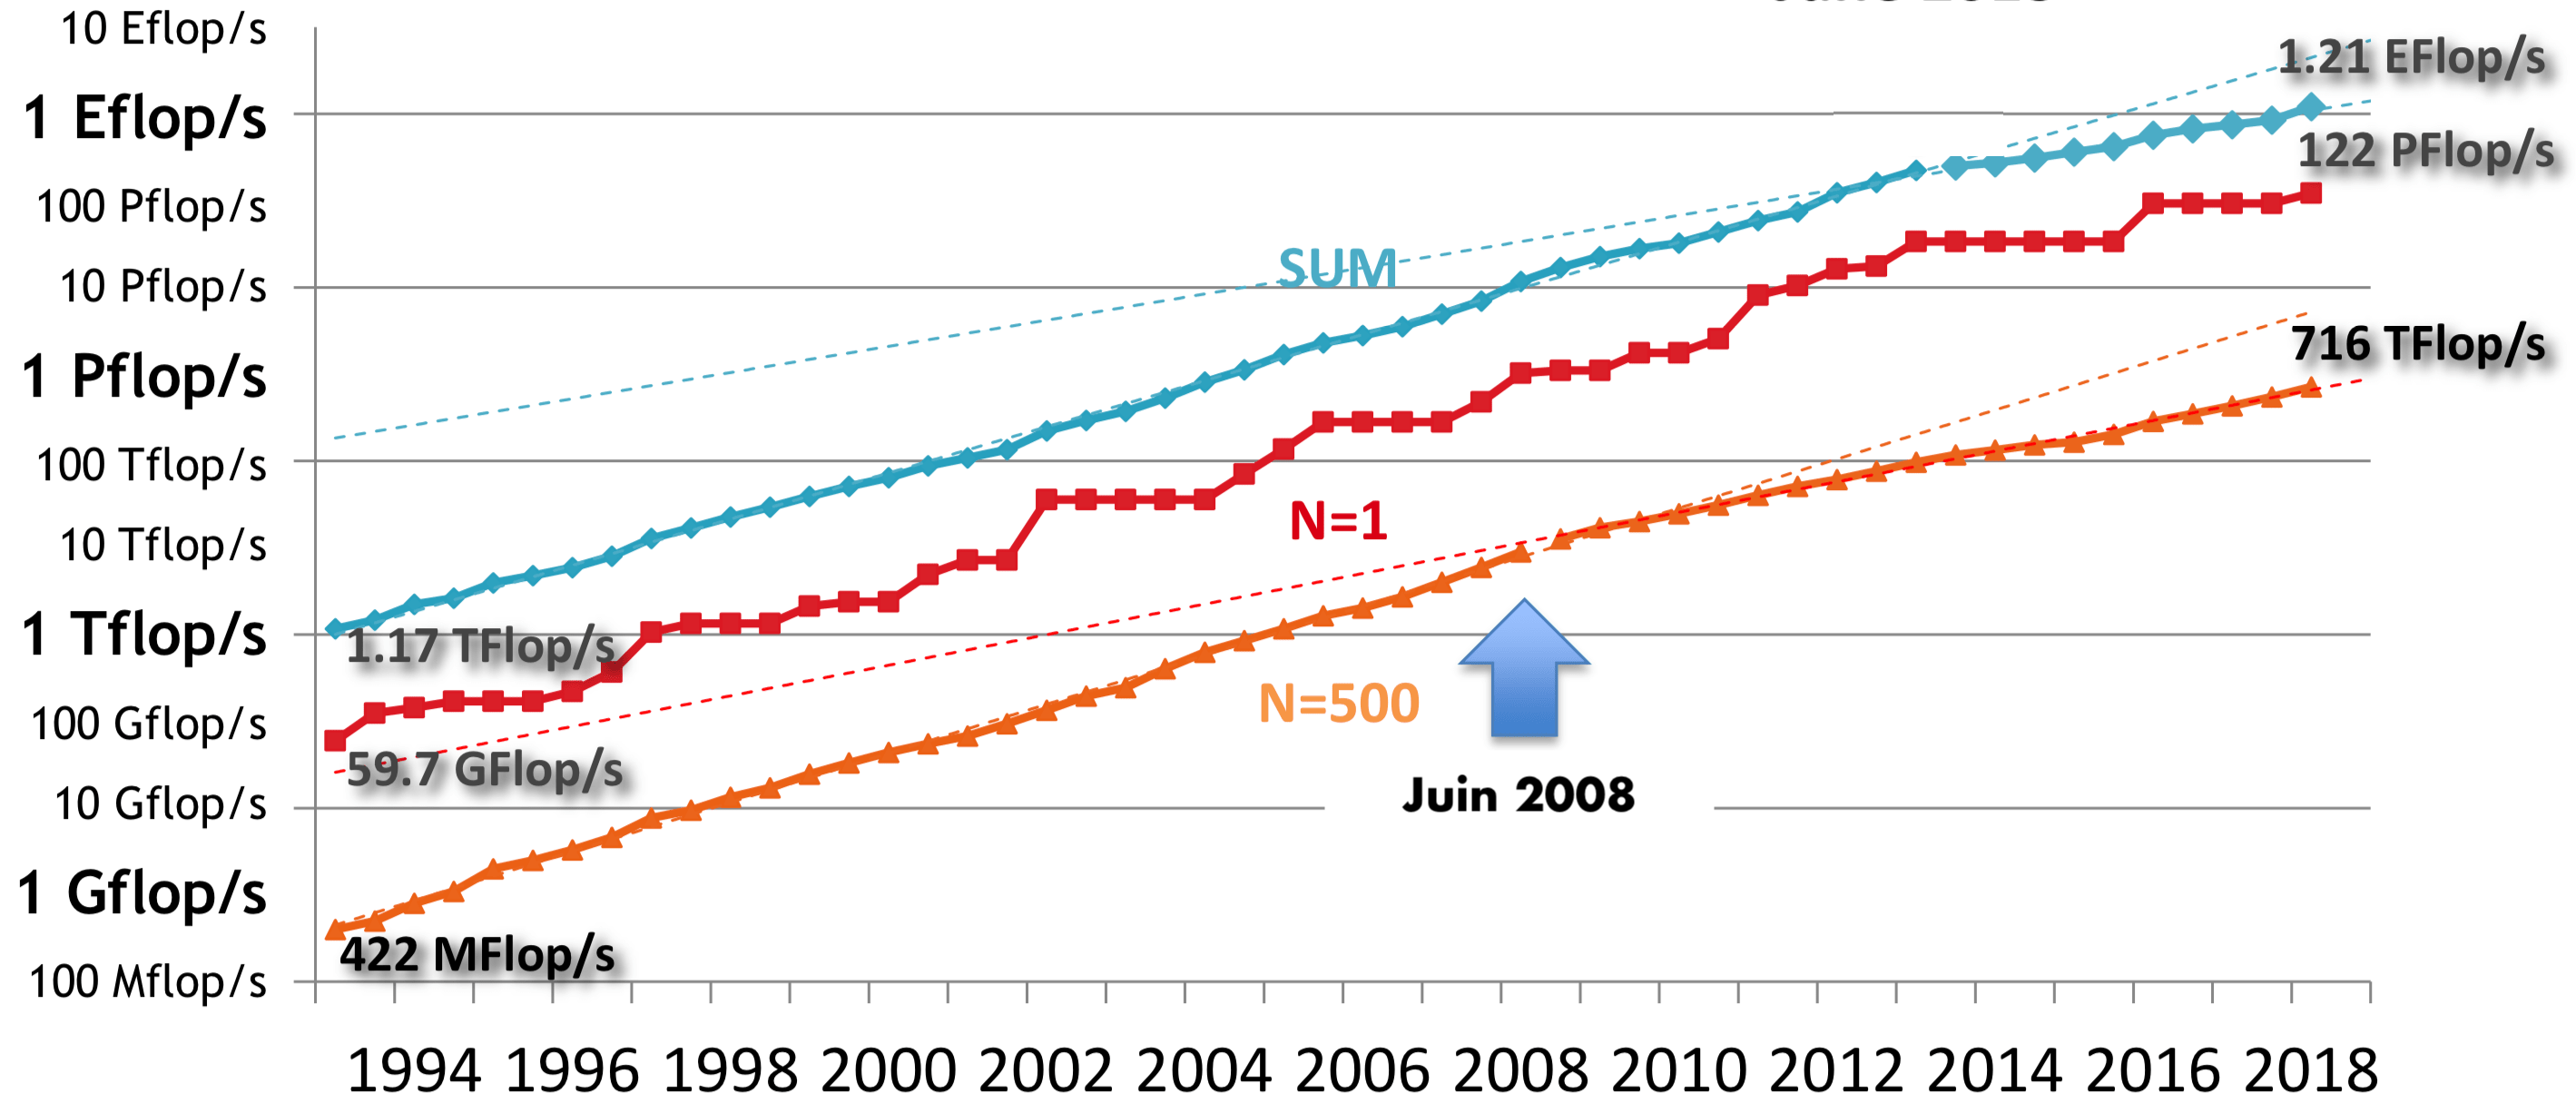
\includegraphics[width=14cm]{images/Top500_Poor.png}
            \caption{\label{fig:Top500_Poor} Évolution des performances du Top500 en \gls{FLOPS} grâce à l'aide du benchmark HPL. Le graphe présente la puissance cumulée des 500 ordinateurs (en bleu), celle du premier (en rouge) et celle du dernier (en orange)\protect\footnotemark.}
            \end{figure}
            \footnotetext{Graphique tiré de \url{https://www.top500.org/news/112019-highlights/}}
    
                
%%%%%%%%%%%%%%%%%%%%%%%%%%%%%%%%%%%%%%%%%%%%%%%%%%%%%%%%%%%%%%%%%%%%%%%%%%%% 
            
        \paragraph{Déséquilibre des microarchitectures.}  
        Si l'utilisation de processeurs multicoeurs a permis de continuer d'augmenter la performance des processeurs malgré la faible évolution des fréquences, l'ajout de coeur a lui aussi atteint ses limites. En effet, comme démontré dans la \autoref{sec:parallele_perf}, l'augmentation des niveaux de parallélisme atteint elle aussi ses limites lorsque les applications contiennent des zones de codes séquentiels. Même des applications comme le benchmark \verb|HPL| sont impactés par \textbf{la loi d'Amdahl}, et l'ajout de coeurs s'est révélé de moins en moins efficace. On remarque sur la \autoref{fig:evo_proc} que le nombre de coeurs a peu évolué ces dix dernières années. Dans l'\aref{sec:memory_wall_gap}, nous discutons de la disparité des évolutions technologiques des processeurs d'une part et des mémoires d'autre part. Cet écart a évolué au fil des années et il est aujourd'hui appelé \textit{mur de la mémoire} \cite{Rojas1997}  (\textit{memory wall} ou \textit{memory gap}). Les premiers processeurs étaient limités par la puissance de calcul, aujourd'hui il est très rare que la performance des applications de calcul haute performance soit limitée par les FPU. L'ajout supplémentaire de coeurs est donc moins bénéfique, car le ratio de bande passante disponible par coeur diminue. 
        Si on regarde l'évolution des performances des différentes parties du système, on peut constater de réelles différences:             
        \begin{itemize}                 
            \item La performance calculatoire des processeurs (le nombre d'opérations flottantes réalisables par cycle) a \textbf{augmenté de 50\%} en moyenne par an.
            \item La bande passante entre le processeur et la mémoire a augmenté de 23\% par an                 
            \item La latence des requêtes mémoires a \textbf{diminué de 4\% } par an                 
            \item La bande passante sur le réseau a \textbf{augmenté de 20\%} par an             
        \end{itemize}
            
            La \autoref{pic:cpuvsmemory2} montre le déséquilibre entre ces deux parties fondamentales des architectures Von Neumann. Ce déséquilibre empêche aujourd'hui le système mémoire de transférer les données suffisamment rapidement pour que la totalité des unités de calculs soit constamment active. Pourtant, 50\% des broches d'un processeur récent sont allouées au système mémoire. Ainsi, bien que les performances de calculs des processeurs s'améliorent, les applications ne peuvent pas en bénéficier. La plupart des supercalculateurs atteignent rarement une efficacité de 80\% sur une application simple comme Linpack \cite{Dongarra2003}. Pour des applications réelles, cette efficacité est encore plus faible, parfois inférieure à 10\% \cite{Oliker2005}.
            
            \begin{figure}             \center             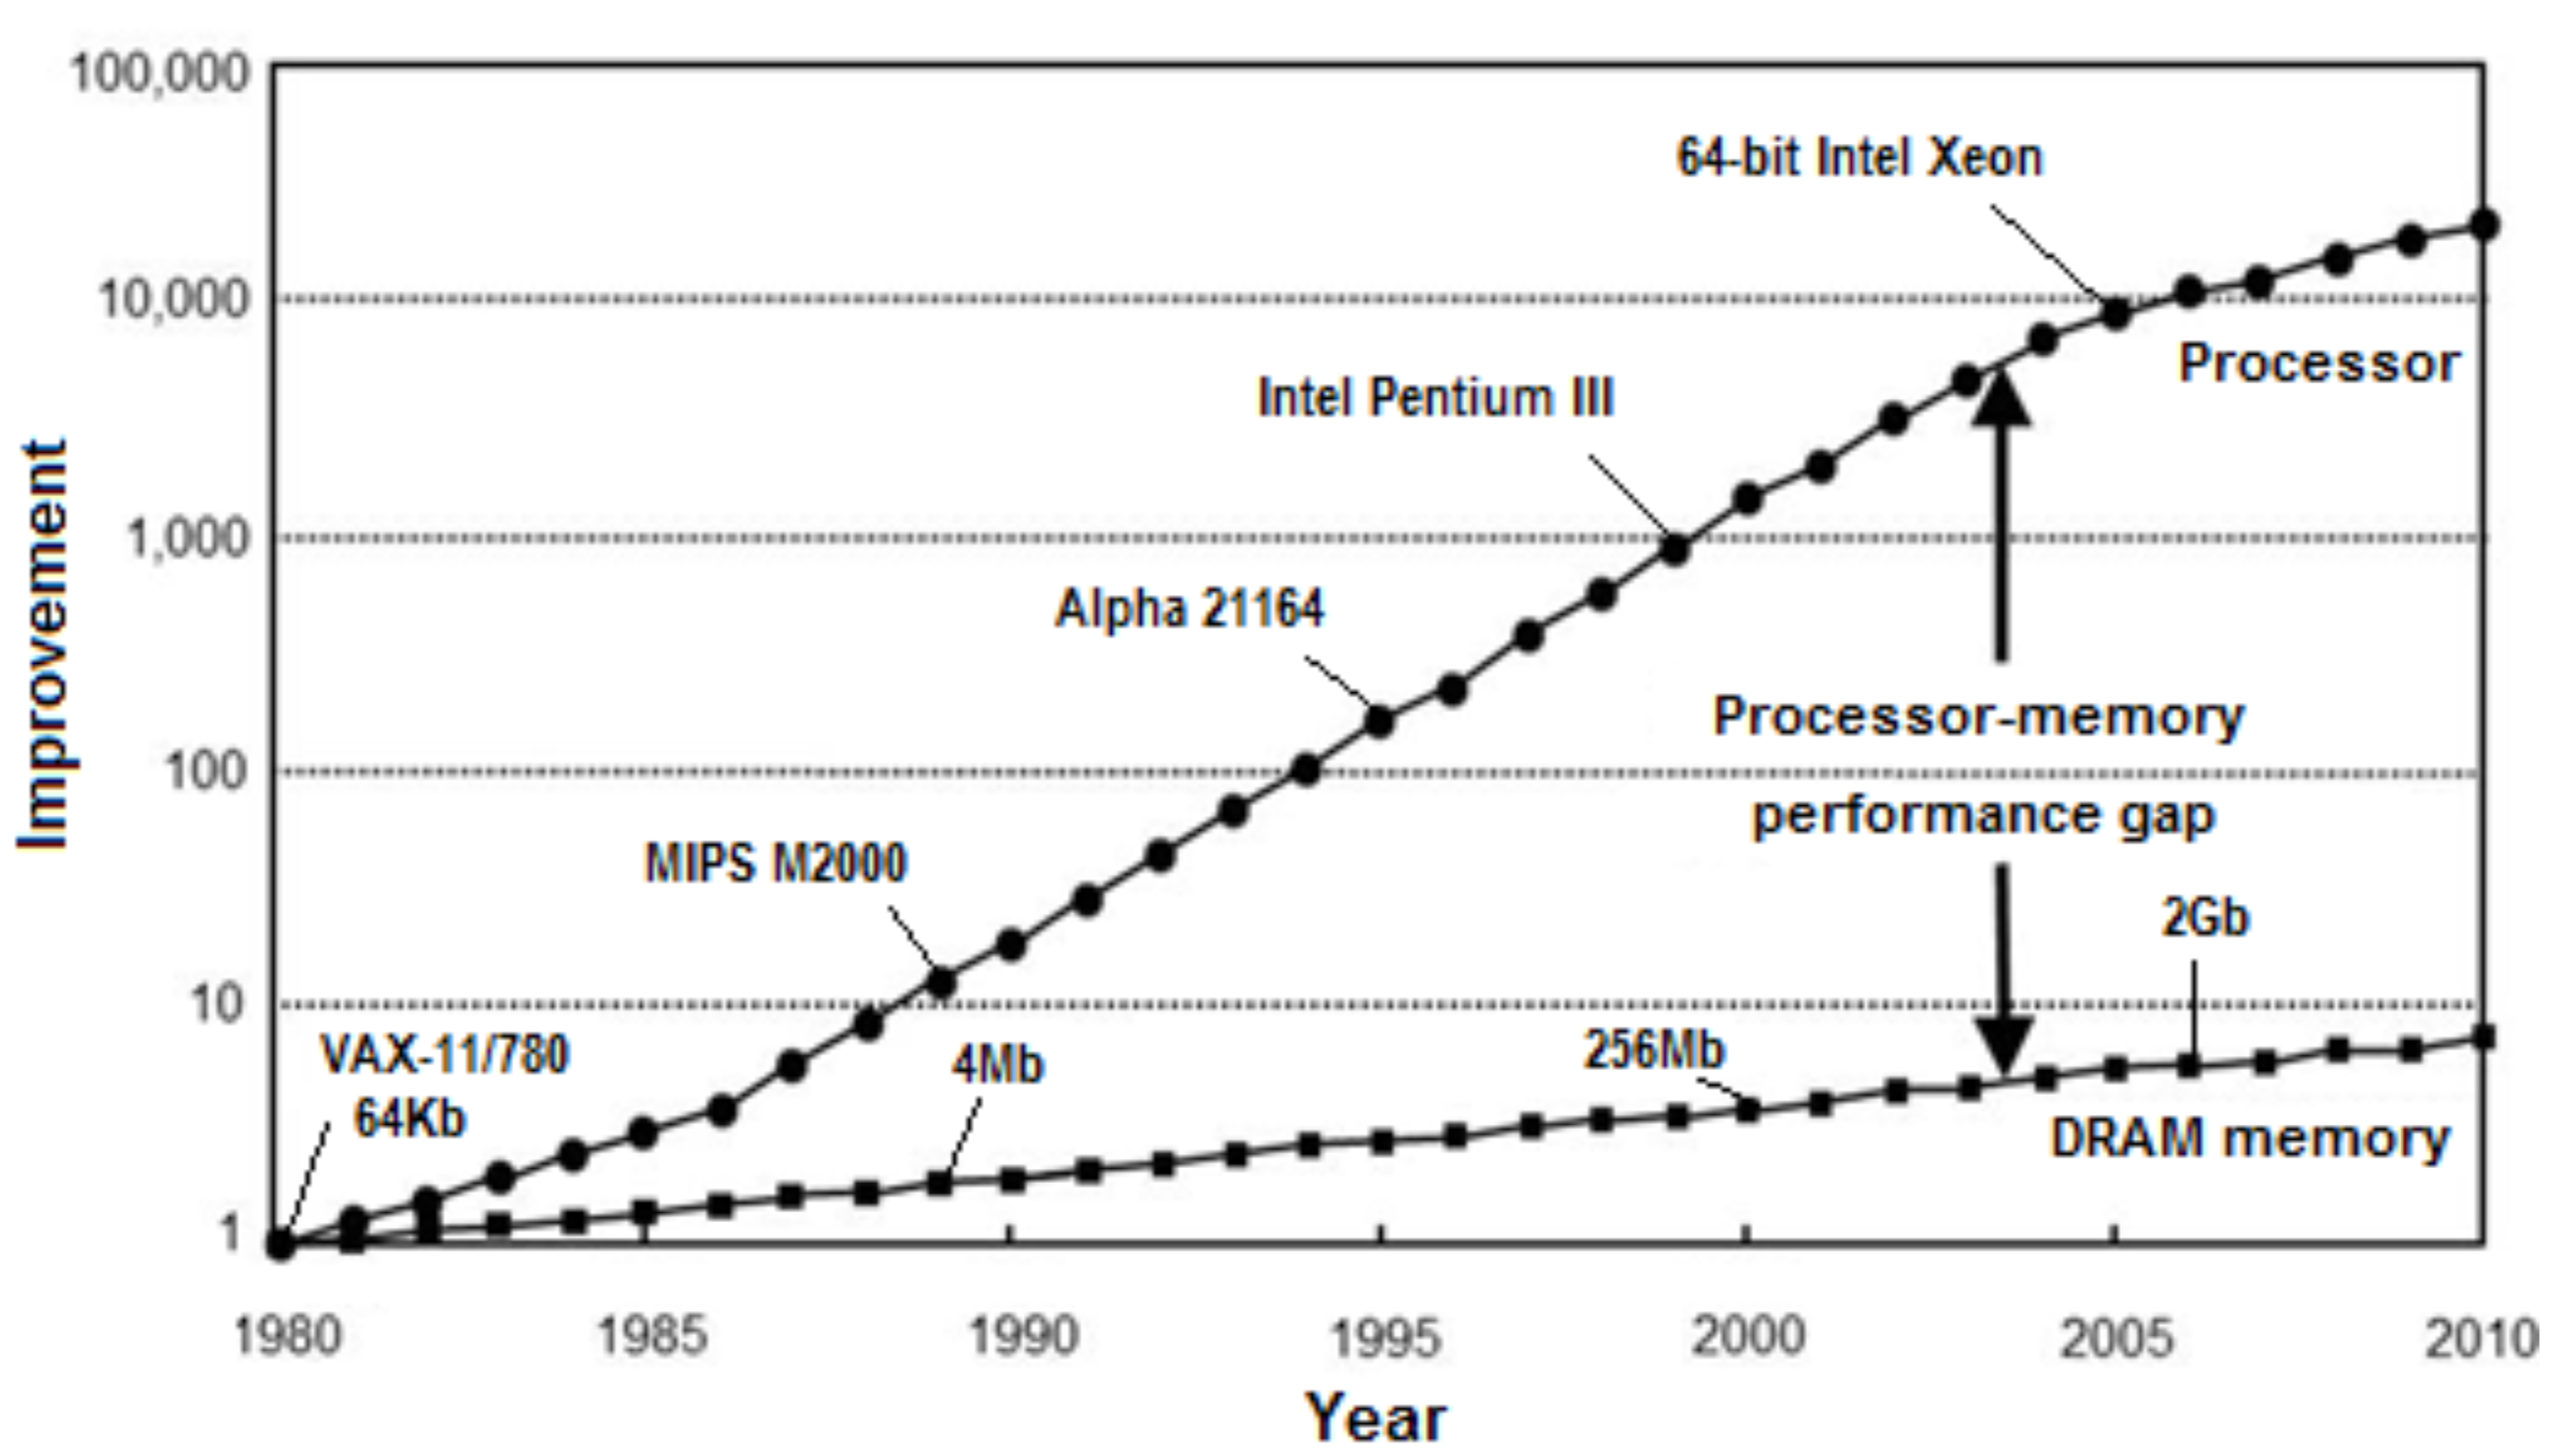
\includegraphics[width=10cm]{images/cpu_cpu_vs_memory.png}             \caption{\label{pic:cpuvsmemory2} Progression de la performance des processeurs et des mémoires. La performance de plusieurs générations de processeurs a été mesurée à l'aide du benchmark SPECint \cite{Efnusheva2017ASO}. La performance mémoire est représentée par la latence des accès mémoire (CAS et RAS) des mémoires DRAM.}
            \end{figure}
            
            Le déséquilibre des microarchitectures se fait d'autant plus ressentir lorsque des centaines de serveurs sont réunis. La \autoref{fig:unbalance_flop_io} montre l'évolution de la puissance des serveurs et du débit mémoire des 10 premiers supercalculateurs du Top500. Grâce aux évolutions des processeurs (voir \autoref{sec:proc_evo_2012}) et l'utilisation des GPUs, la puissance des serveurs a été multipliée en moyenne par 65 entre 2010 et 2018 (courbe bleue). Pendant la même période, le débit des communications inter serveur n'a lui augmenté que d'un facteur 4.8 (courbe rouge). Ainsi, le ratio entre la puissance de calcul des serveurs et le débit de communication (byte par \gls{FLOP}) n'a fait que diminuer. Entre 2017 et 2018, ce ratio a diminué d'un facteur 8 pour les deux premiers supercalculateurs du Top500 (respectivement Sunway Taihulight et Summit). Pour des applications nécessitant de grandes communications interserveur, ce ratio très faible les empêche d'atteindre plus d’une fraction de la performance disponible.
            
            \begin{figure}             \center             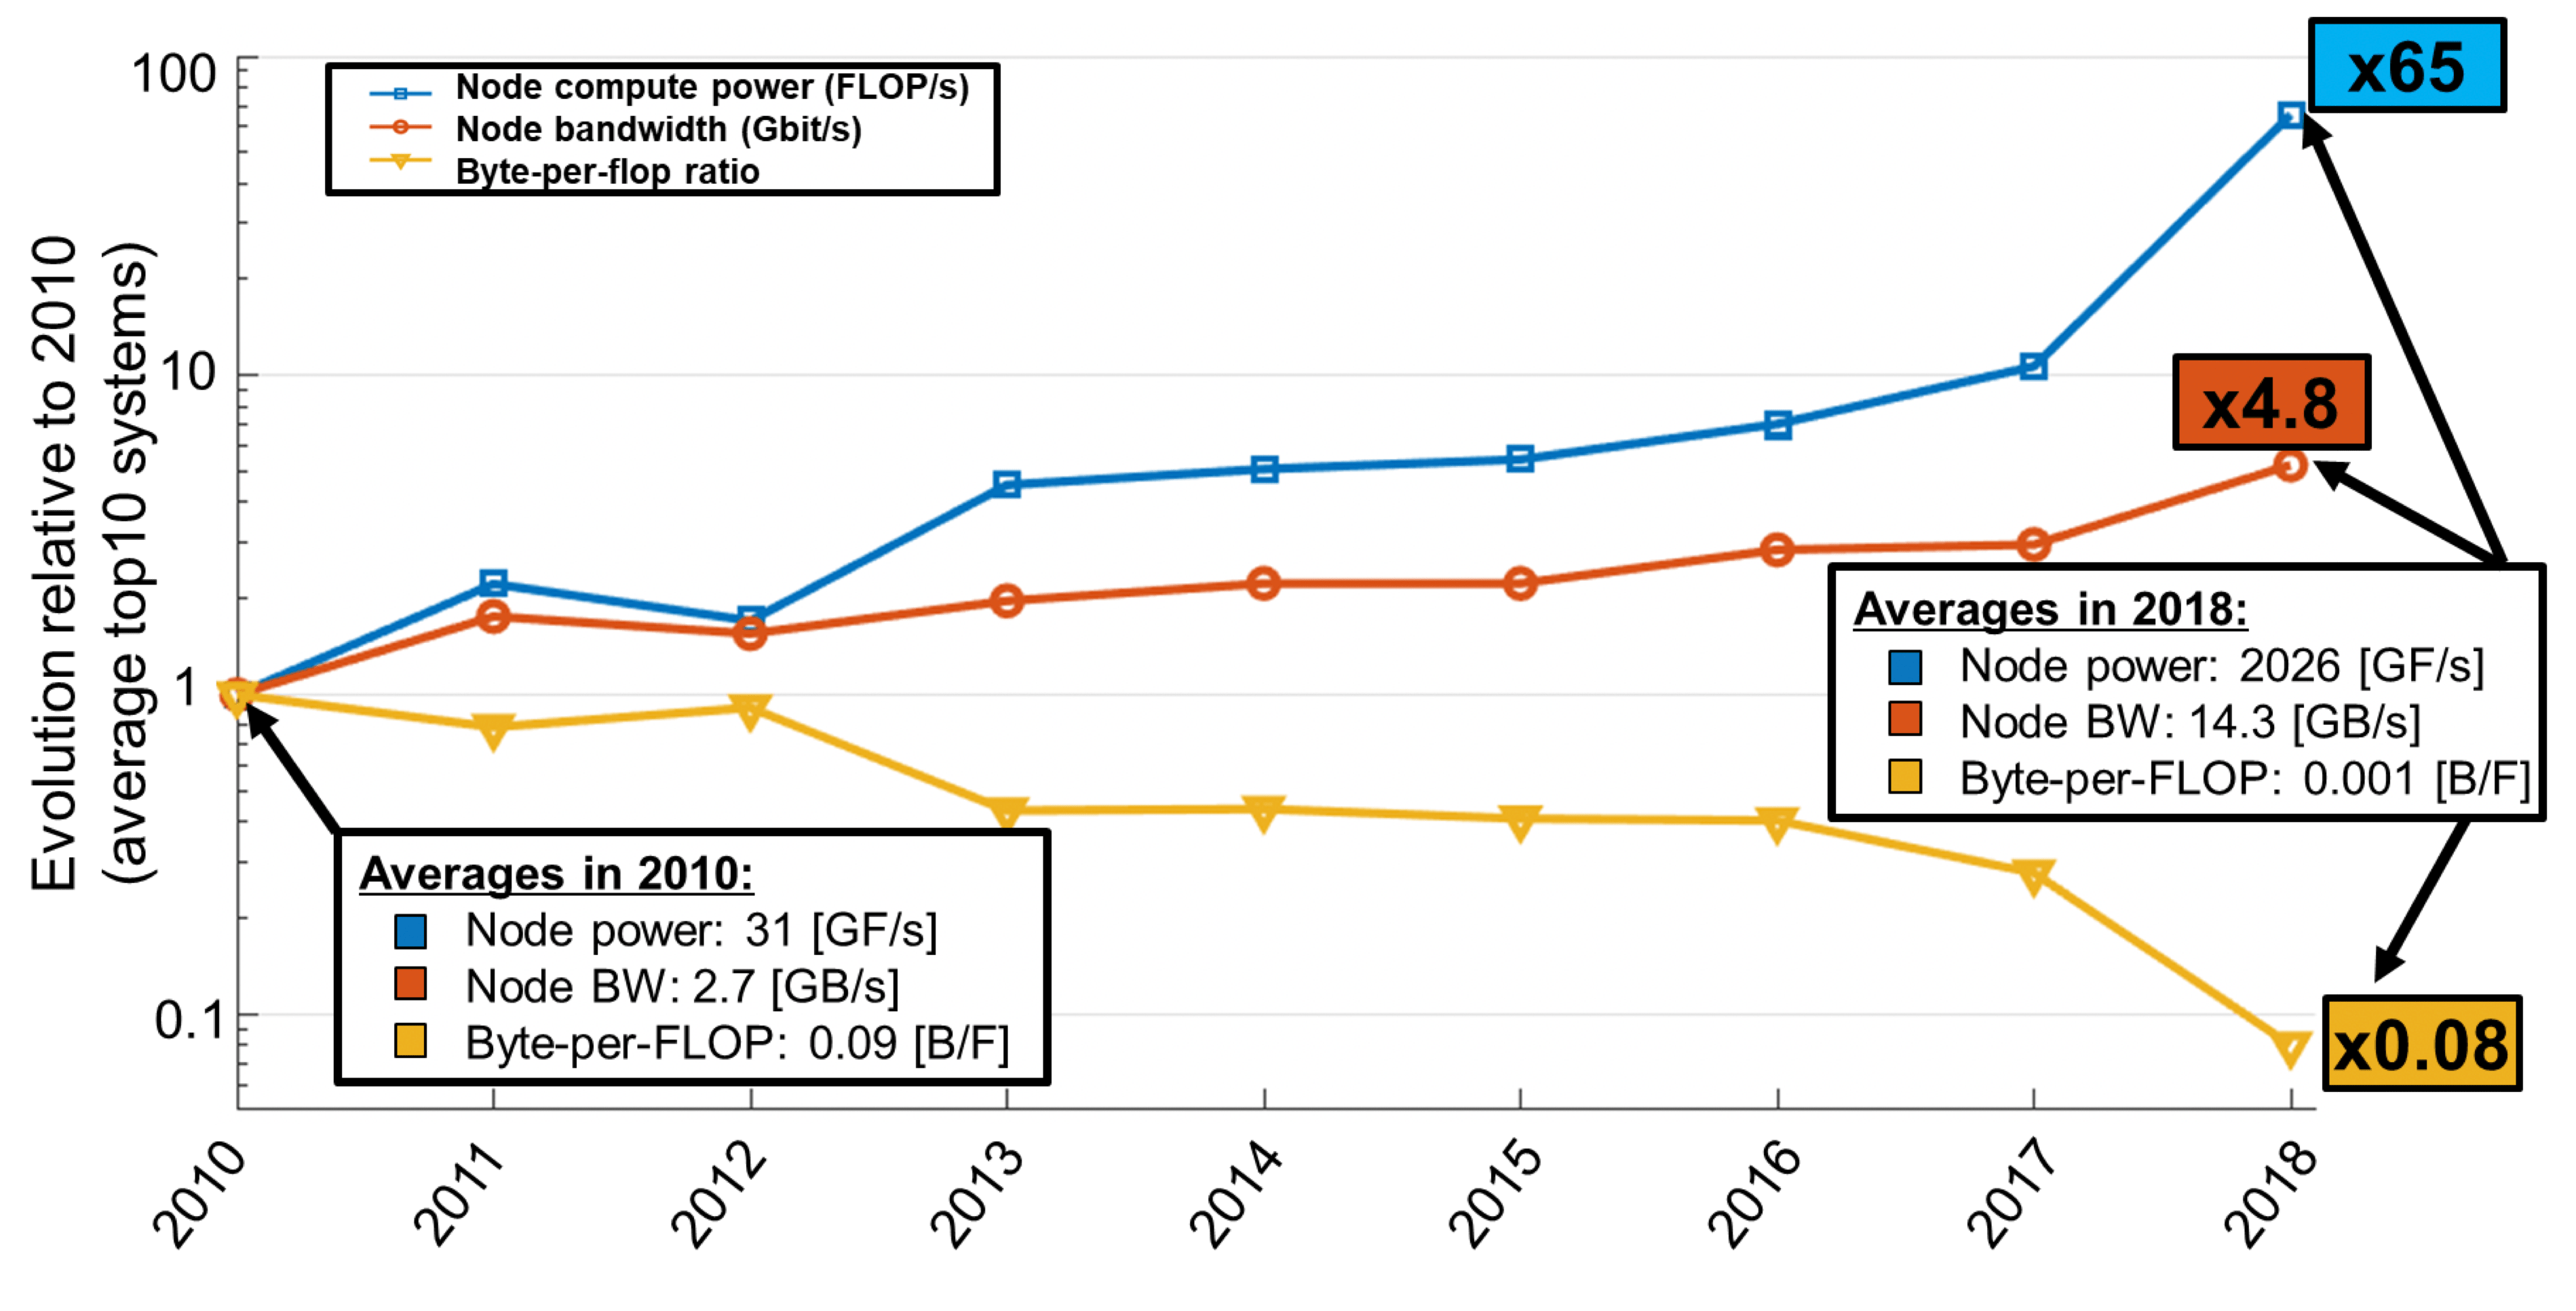
\includegraphics[width=12cm]{images/unbalance_flop_io.png}             \caption{\label{fig:unbalance_flop_io}Évolution des 10 premiers supercalculateurs du Top500 de 2010 à 2018: la puissance de calcul des serveurs (FLOP/s) en bleu, le débit de communication entre les serveurs (Gbit/s) en orange, ainsi que le ratio entre ces deux caractéristiques (byte par \gls{FLOP}) en jaune. (graphique tiré de la conférence IPDPS 2018 \cite{Bergman2018})}             \end{figure}
 
 
\subsection{Le futur du HPC}
%%%%%%%%%%%%%%%%%%%%%%%%%%%%%%%%%%%%%%%%%%%%%%%%%%%%%%%%%%%%%%%%%%%%%%%%


    \begin{fancyquotes}
    Peu importe la puissance qu'atteindront les processeurs, le logiciel trouvera toujours une façon d'utiliser cette puissance. Construisez un processeur 10 fois plus rapide, et la partie logiciel trouvera toujours 10 fois plus à faire (ou le fera 10 fois moins efficacement)  \cite{Sutter2005}.
    \end{fancyquotes}
 
    \subsubsection{Situation du HPC en 2020}
    %%%%%%%%%%%%%%%%%%%%%%%%%%%%%%%%%%%%%%%%%%%%%%%%%%%%%%%%%%%%%%%%%%%%%%%%

   
        %EVO DES PERFORMANCES IT
        
        La performance des supercalculateurs et des technologies de l'information n'a fait qu'augmenter au cours de ces 30 dernières années. Une montre connectée récente apporte une puissance de calcul deux fois supérieure à celle du supercalculateur Cray-2, le plus puissant des supercalculateurs de 1985. Un GPU moderne tel que le GPU Nvidia V100 délivrant une puissante de 7.5 téraFLOPS ($10^{12}$ \gls{FLOPS}) serait classé à la 30e place du Top500 de 1994.

        %HPC: PLUS QUE DU CALCUL, UN MODE DE VIE
            
        L'évolution des performances des matériels informatiques a largement transformé le mode de vie de nos sociétés. Les produits du HPC sont présents dans nos vies quotidiennes: nous nous déplaçons grâce à l'essence extraite à l'aide de la modélisation des fonds marins, lorsque nous consultons la météo ou lorsque nous ingérons un médicament. Le HPC a un réel impacte sur nos vies, les rendant plus sécurisées en prévoyant précisément des catastrophes naturelles. 
        Le HPC est un outil inhabituel, car il ne se limite pas à un domaine particulier. La majorité des domaines scientifiques ont recours à des calculateurs. 
        %IL Y A UNE DEMANDE DE PLUS DE CALCUL
  
        Suite à la forte évolution de la performance des supercalculateurs, nous pouvons nous demander s'il est nécessaire de continuer à construire des infrastructures toujours plus puissantes. La variété et la complexité des problèmes qui peuvent être traités dépendent directement de la puissance de calcul disponible. L’apprentissage profond (\textit{deep learning}) en est un bon exemple. Dès 1989, Yann LeCun améliorait déjà la rétropropagation \cite{Treibig2012a} et utilisait les réseaux neuronaux convolutionnels \cite{LeCun1989}. Mais à cette époque les GPGPU n'étaient pas disponibles et les CPU étaient loin d'être assez puissants pour exécuter ces algorithmes, même sur les données limitées disponibles à cette époque. Dans les années 2010, les GPU sont devenus suffisamment puissants pour permettre l'exécution de ces algorithmes.
        
        
        La mise au point de plateformes plus puissantes va permettre aux entreprises d'être plus compétitives et aux équipes de recherches de réaliser de nouvelles découvertes. Un grand nombre de domaines scientifiques vont pouvoir profiter de telles puissances de calculs: découverte de nouveaux matériaux, simulations de réactions chimiques ou encore pour analyser les résultats d'expériences lourdes comme celles réalisées au Grand collisionneur de hadrons \cite{10.1007/978-3-319-67630-2_52}. La recherche pour le climat va aussi bénéficier de telles architectures et permettre de comprendre les dérèglements climatiques, anticiper la hausse des océans et élaborer de meilleurs modèles. Les simulations permettront également d'améliorer l'efficacité et la sécurité des réacteurs nucléaires \cite{Simon2007}. En astrophysique, elles permettront d'étudier des phénomènes encore incompris comme la formation des trous noirs \cite{10.1007/978-3-642-38750-0_2}. L'accès à des infrastructures plus puissantes permettra de poursuivre les avancées réalisées dans le domaine de la physique quantique. Ces découvertes pourront permettre de construire d'autres plateformes de calculs appelées ordinateurs quantiques.
        
         
    \subsubsection{Nécessité de construire des plateformes plus puissantes}\label{sec:3_motivations}
    %%%%%%%%%%%%%%%%%%%%%%%%%%%%%%%%%%%%%%%%%%%%%%%%%%%%%%%%%%%%%%%%%%%%%%%%

        \begin{fancyquotes}
        La taille des données double tous les deux ans, et d'ici 2020, les données que nous générons et copions annuellement atteindront 44 Zettabytes ($10^{21}$ bytes) \cite{Zhang2017}.
        \end{fancyquotes}
    
        Aujourd'hui, de nombreuses applications sont prêtes, mais ne peuvent pas être exécutées en un temps raisonnable avec les moyens de calculs disponibles. Actuellement il est possible de simuler des réactions chimiques de quelques nanosecondes et sur de petits volumes. Avec la construction de supercalculateurs plus puissants, il sera possible de réaliser des simulations plus longues et plus précises. Nous discutons dans cette section de trois facteurs importants qui motivent la nécessité de poursuivre le développement de plateformes plus performantes que celles actuellement en notre possession: l'explosion du volume de données à traiter, la complexification des analyses et le besoin d'obtenir des résultats rapidement.

        
        \paragraph{Tsunami de données.} 
            
            Suite aux évolutions des technologies des semi-conducteurs, nous assistons depuis le début des années 2010 à l'explosion des quantités de données générées (voir \autoref{fig_edl_bigdata}). Grâce aux nanotechnologies, il est possible de produire des capteurs à très faible coût. La consommation électrique de ces matériels étant faible, ces capteurs sont installés partout. L’Internet des Objets (IOT) interconnecte ces milliers de capteurs pour générer de grands volumes de données (\textit{big data}).  Les évolutions récentes de la domotique ont permis d'installer des capteurs dans toute la maison: que ce soit pour gérer les lumières, le chauffage, l'ouverture des volets ou même l'allumage de la cafetière. En 2018, Ericsson comptait plus de 5 milliards d'abonnés au téléphone dans le monde\footnote{Source: \url{https://www.usinenouvelle.com/article/5-4-milliards-d-abonnes-au-telephone-mobile-dans-le-monde.N739439}}. Ces téléphones peuvent aujourd'hui suivre nos moindres faits et gestes, générant de grandes quantités de données. Celles-ci peuvent ensuite être utilisées par différentes applications pour étudier les déplacements des habitants d'une ville ou proposer des annonces ciblées. Les villes elles-mêmes se sont dotées de milliers de capteurs permettant le développement de nombreuses applications comme le suivi du trafic routier \cite{bonhomme:hal-01334670}, l'utilisation des transports en commun, ou de suivre le recyclage des déchets dans un quartier \cite{Rebelles2018}. Ce grand volume de données produit aujourd'hui et qui va s'intensifier dans les années futures est le principal challenge des systèmes d'informations.
        
              
            \begin{figure}
            \center
            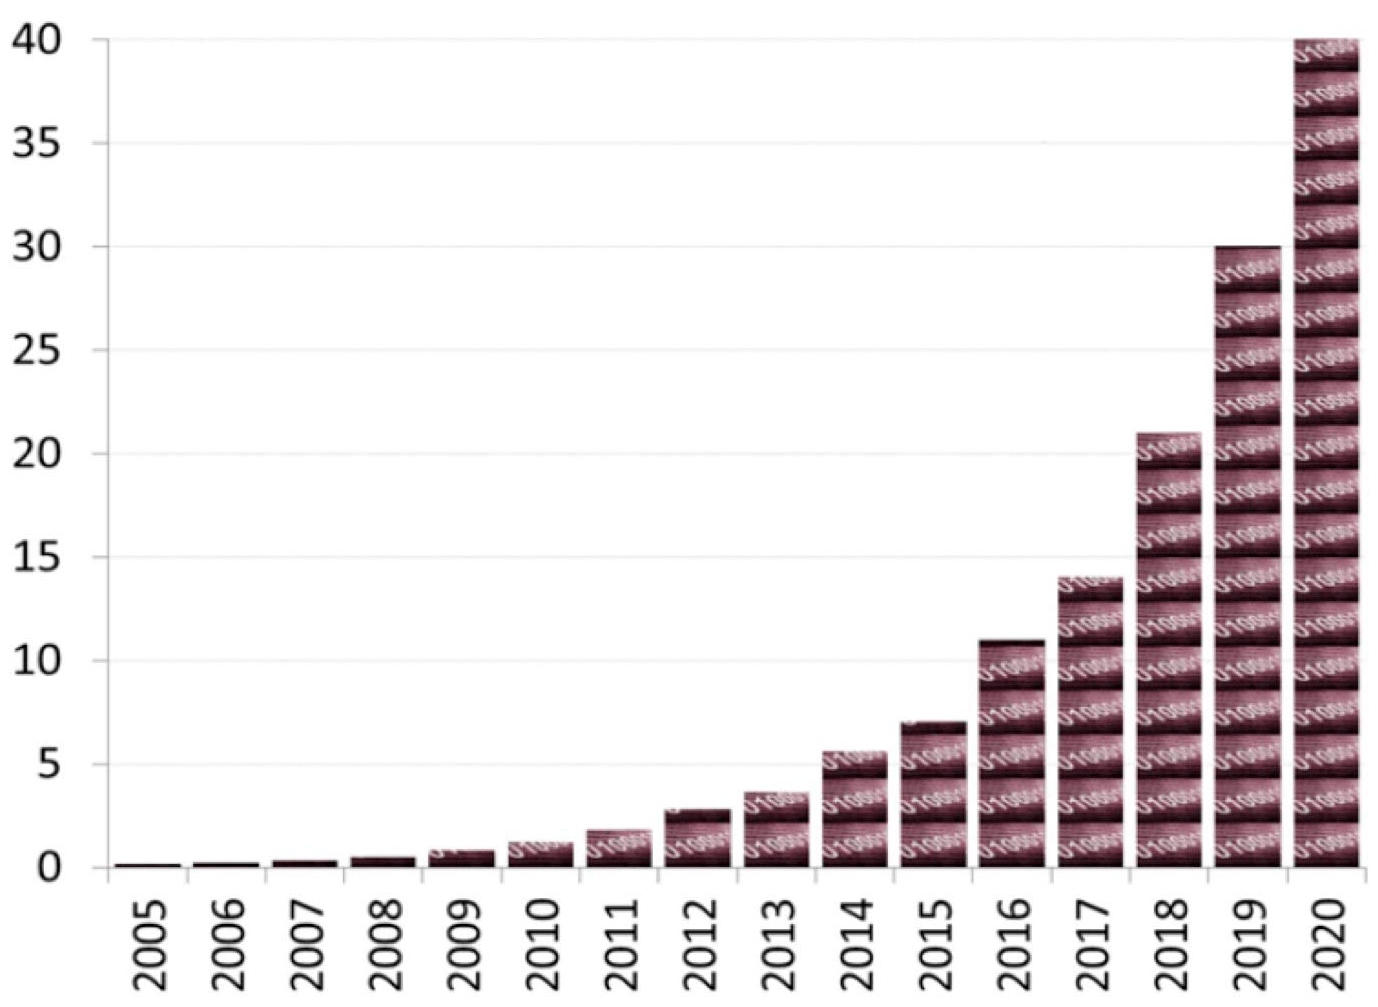
\includegraphics[width=10cm]{images/edl_bigdata.png}
            \caption{\label{fig_edl_bigdata} Le volume de données généré chaque année devrait atteindre 40 Zettabytes en 2020 \cite{Simoudis2016}}
            \end{figure}
        
        

            
        \paragraph{Complexité des calcus.} 
             Aujourd'hui, la valeur ne provient plus de la capacité à produire ces données, mais de la capacité d'en extraire une valeur avec des algorithmes de \textit{big data} et d'apprentissage machine. Les algorithmes d'intelligence artificielle nécessitent d'être entraînés sur des jeux de données pour pouvoir ensuite prendre les décisions adaptées. En 2018, OpenAI a constaté que la puissance de calcul utilisée pour entraîner les plus grands modèles d'IA avait doublé tous les 3,4 mois depuis 2012 (voir \autoref{fig_edl_ai_compute}). Dans le domaine de la santé, de telles infrastructures pourront permettre d'extraire et analyser toutes les informations de millions de patients atteints de maladies grâves.  Il sera alors possible de mieux comprendre les symptômes menant au développement d'un cancer ou d'une maladie cardiaque. 
             Pour obtenir des résultats dans des temps raisonnables, ces applications nécessitent d'avoir accès à des plateformes plus puissantes de plusieurs facteurs que celles existant actuellement. Avec l'analyse des données obtenues grâce aux montres connectées, il sera alors possible d'anticiper les maladies cardiaques.
             
            \begin{figure}
            \center
            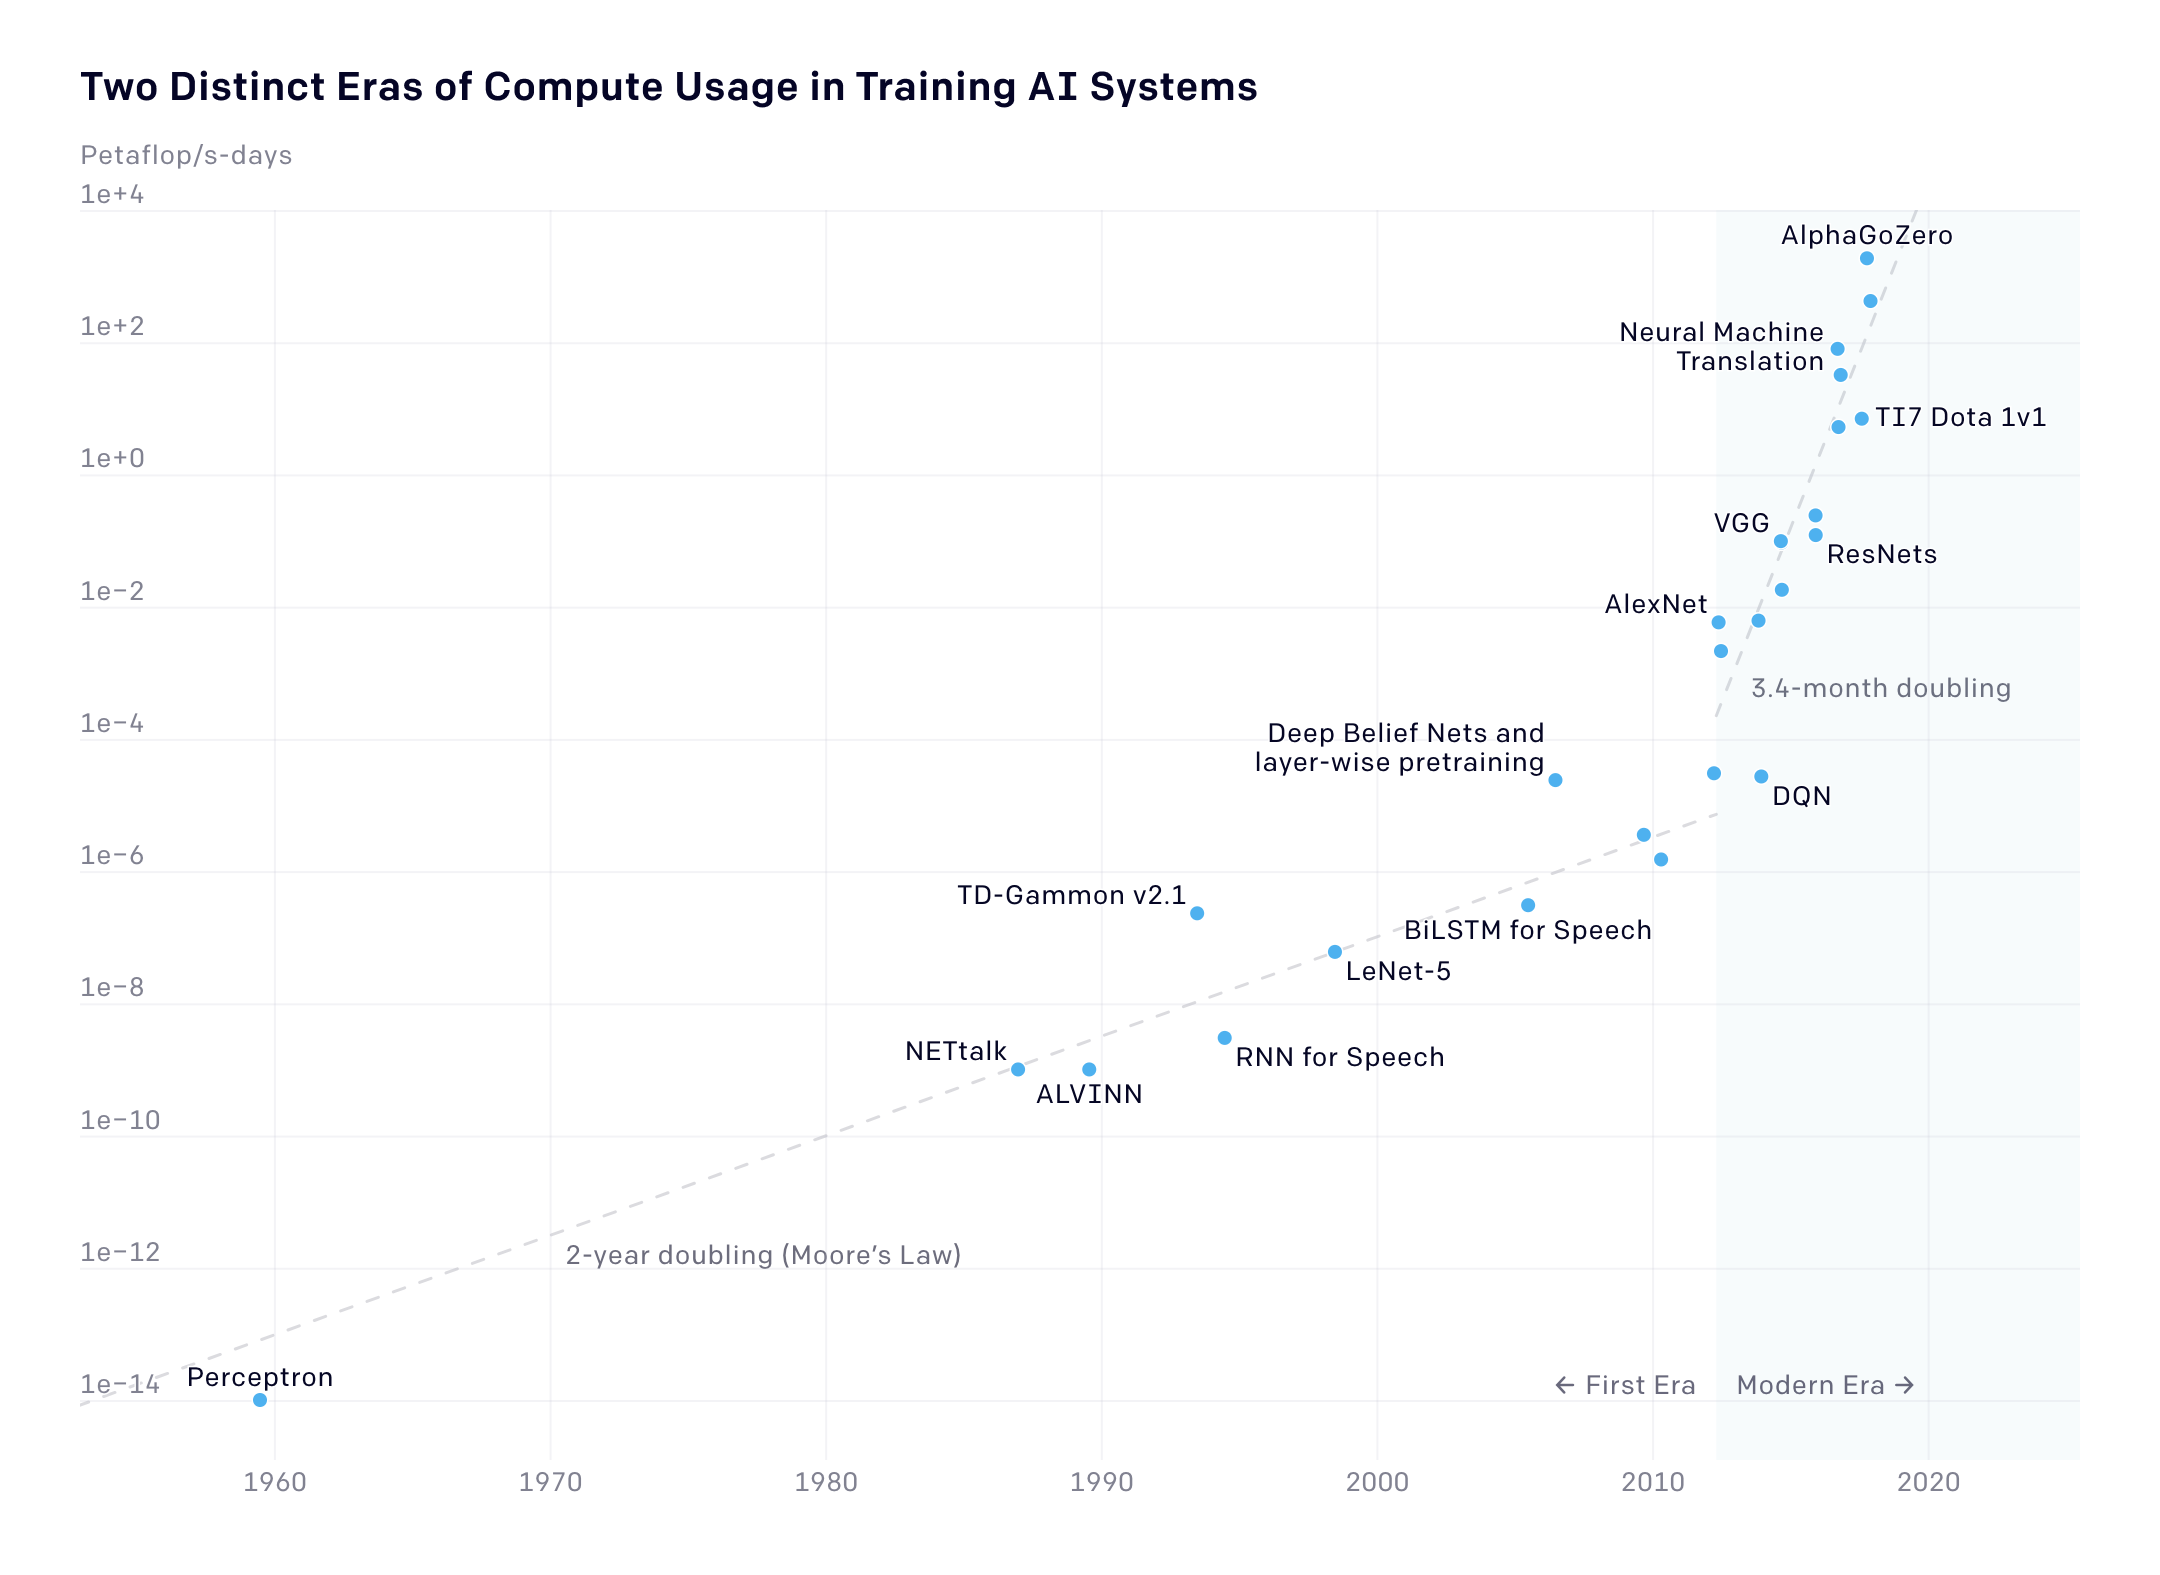
\includegraphics[width=14cm]{images/edl_ai_compute.png}
            \caption{\label{fig_edl_ai_compute} Quantité totale de calcul (en pétaFLOPS ($10^{15}$ \gls{FLOPS})) nécessaire chaque jour pour entraîner les différents réseaux de neurones \cite{amodei2ai}.}
            \end{figure}

        \paragraph{Temps de traitement.} 
        
            La troisième raison qui motive le développement de nouvelles plateformes plus puissantes est de réduire le temps d'exécution des applications. Une fois la donnée produite, sa valorisation diminue dans le temps. La météo est un très bon exemple d'application ne pouvant pas excéder un certain temps de traitement si les prédictions veulent être données suffisamment rapidement. Par exemple, pour permettre aux voitures connectées d'identifier un danger, l'action correspondante doit être prise le plus rapidement possible. La possibilité d'envoyer les données à traiter à un supercalculateur n'est alors pas envisageable. L'accès à des plateformes plus puissantes est alors nécessaire pour traiter cette quantité de données dans des temps raisonnables. En plus d'améliorer les performances des supercalculateurs, l'architecture complète des plateformes doit être repensée. Pour traiter efficacement le volume de données générées, plusieurs travaux montrent qu'il est indispensable de repenser notre façon de stocker, déplacer et analyser ces données \cite{Saltz2018, Chen2014, Nahrstedt2017, GeoffreyFoxJhaShantenu2015}.
  
 
    \subsubsection{Exascale}\label{sec:exascale}
    %%%%%%%%%%%%%%%%%%%%%%%%%%%%%%%%%%%%%%%%%%%%%%%%%%%%%%%%%%%%%%%%%%%%%%%%
        
      
        %Exascale Definition maison             
        
        Le terme \gls{exascale} est utilisé pour définir la prochaine génération de supercalculateurs capable d'atteindre une performance de \gls{exaFLOPS}. Cette performance devra être mesurée à l'aide du benchmark High-Performance Linpack (HPL \cite{Dongarra2003}). En effet, certains supercalculateurs sont déjà capables d'atteindre de telles performances sur des applications plus simples. En 2018 le supercalculateur Summit était capable d'exécuter $1.2 * 10^{18}$ opérations par seconde. L'application utilisée était une application d'apprentissage en profondeur utilisée pour étudier les déchets nucléaires.  Cette application n'utilise que des opérations en simple précision. Le même supercalculateur a pu atteindre une performance de $3.3 \times 10^{18}$ opérations sur une application d'analyse de données, elle aussi en simple précision \cite{Bergman2018}.
         \footnote{\url{https://insidehpc.com/2019/11/deep-learning-on-summit-supercomputer-powers-insights-for-nuclear-waste-remediation/}}. 
        
        Dans la littérature, il est courant d'utiliser le terme \textit{exascale} pour désigner cette nouvelle génération de plateformes 10 fois plus puissantes que les supercalculateurs les plus puissants actuels et 30 fois plus puissants que la moyenne du Top500 de novembre 2019 (33 pétaFLOPS). Le rapport commandé par le département de l'énergie américain en 2014 \cite{Lucas2014} souligne que ce terme ne fait pas référence à la puissance obtenue par le benchmark HPL, mais bien à une plateforme avec 1000 fois plus de capacité que les supercalculateurs existant alors. Dans ces travaux de thèse, nous suivons la même démarche et utilisons le terme exascale pour désigner la plateforme qui permettra d'obtenir les performances souhaitées. La plateforme ne concerne pas seulement le supercalculateur, mais toute la chaîne de traitement de données, depuis sa création jusqu'à son traitement.


\subsection{Défis à relever pour l'élaboration d'une plateforme exascale} \label{sec:challenges}
%%%%%%%%%%%%%%%%%%%%%%%%%%%%%%%%%%%%%%%%%%%%%%%%%%%%%%%%%%%%%%%%%%%%%%%%

    %La course à peta etait dure
        
    Jusqu'à aujourd'hui, quand une piste d'évolution venait à s'épuiser, comme l'évolution de la fréquence des processeurs, d'autres améliorations venaient alors y pallier (augmentation du nombre de coeurs). Dans la \autoref{sec:Top500}, nous avons discuté des principaux freins ayant ralenti l'évolution des performances des supercalculateurs ces 8 dernières années. Depuis plusieurs années, de nombreuses études \cite{Shalf2010, bergman2008exascale, Bergman2011} prédisent les principaux challenges à relever pour la construction d'une plateforme exascale. La plus citée d'entre elles est l'étude menée par le département de l'énergie américain \cite{Lucas2014} qui décrit les dix principaux challenges à relever. Ce rapport met en lumière les nombreuses difficultés que l'industrie rencontre et montre que celles-ci touchent toutes les parties des centres de données (\textit{data center)}): l'énergie, les technologies mémoire et d'interconnexion, la programmation, la gestion ou encore la capacité des applications à utiliser la totalité de la puissance disponible. 
    Il est aussi indiqué que pour construire une telle plateforme dans des coûts financiers et des consommations électriques raisonnables, les dernières avancées technologiques des domaines cités précédemment doivent être intégrées. Le travail de la thèse a en partie été motivé par ces challenges présentés dans les études citées ci-dessus. Dans cette section nous présentons en détail les six principales difficultés que nous avons identifiées. 

    \subsubsection{Les coûts}\label{sec:edl_chal_prix}
    %%%%%%%%%%%%%%%%%%%%%%%%%%%%%%%%%%%%%%%%%%%%%%%%%%%%%%%%%%%%%%%%%%%%%%%%
    %%%%%%%%%%%%%%%%%%%%%%%%%%%%%%%%%%%%%%%%%%%%%%%%%%%%%%%%%%%%%%%%%%%%%%%%

    %MOORE et Transistor $
    
        Dans la \autoref{sec:end_mooore} nous avons expliqué comment la fin de la loi de Moore avait impacté l'évolution des performances des supercalculateurs. Bien que souvent oublié, il est important de rappeler que cette loi est avant tout une loi économique.
        Grâce à l'évolution des procédés de gravure, le nombre de transistors a pu doubler tous les deux ans pendant plus de trente ans alors que le coût des investissements dans les fonderies n'augmentait que de 30\% sur la même période. Cette évolution des prix des fonderies porte le nom de \textit{seconde loi de Moore} ou loi de Rock. À cause des nombreux investissements nécessaires pour développer les nouvelles générations de fonderies nous remarquons que le nombre de transistors achetable pour un budget donné n'évolue plus (voir \autoref{fig:edl_moore_dollars}).
    
        \begin{figure}
        \center
        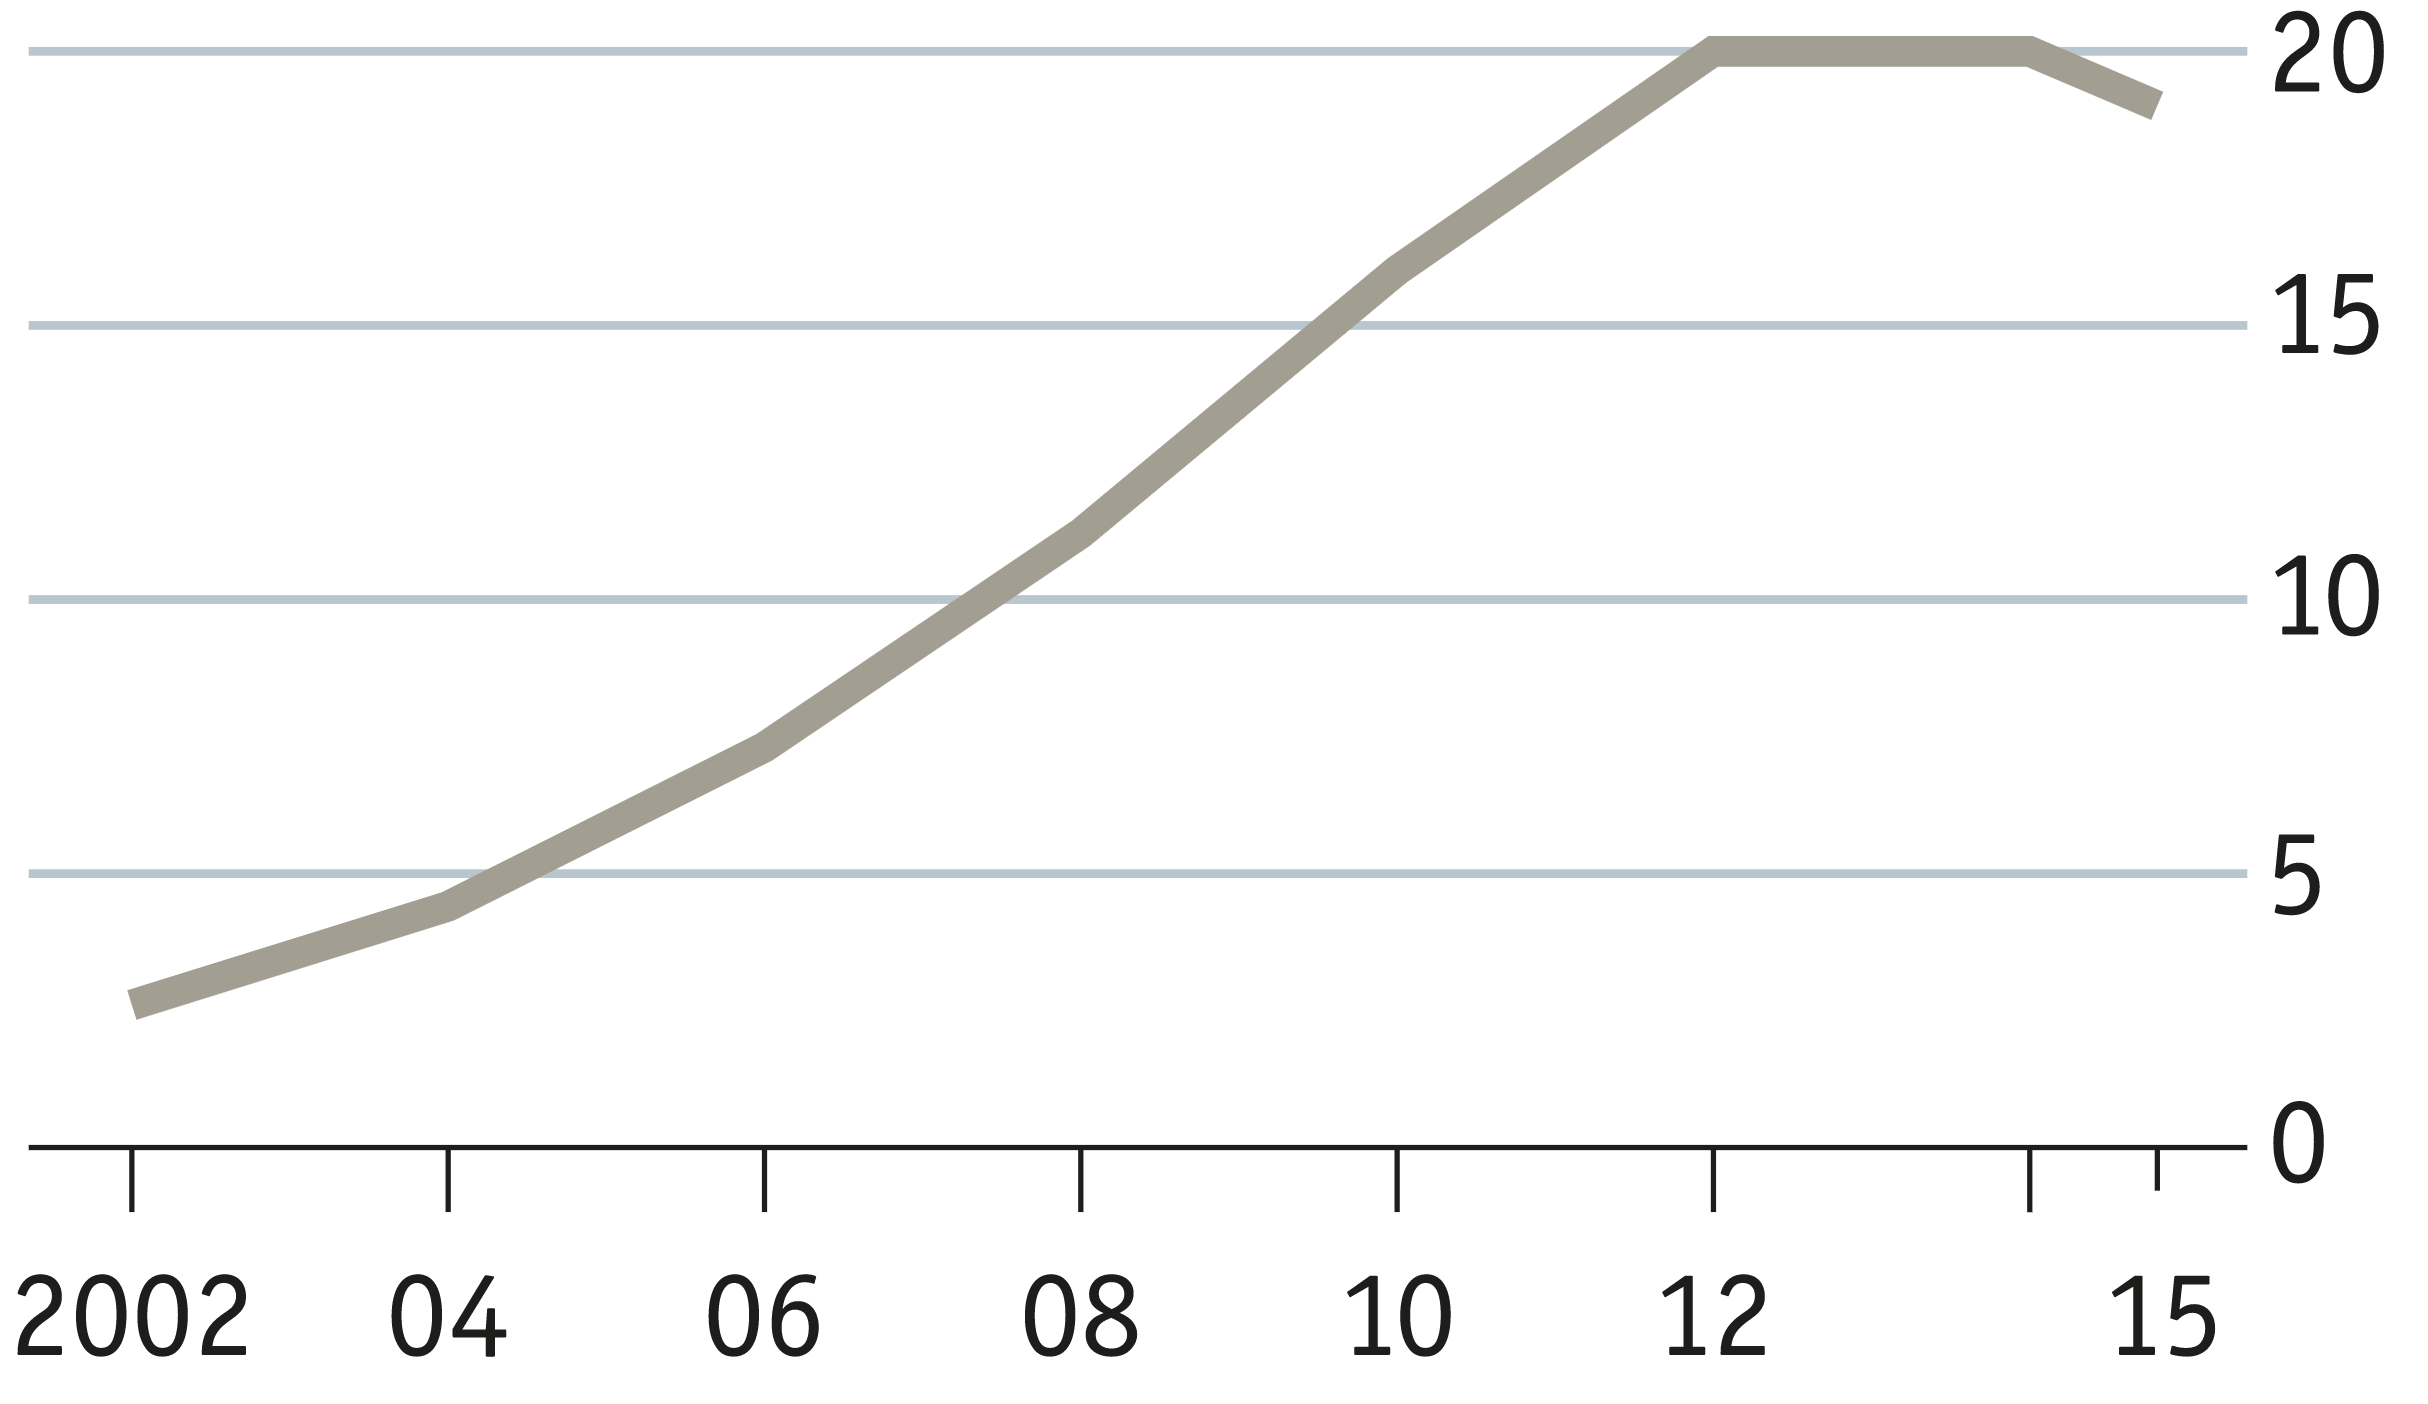
\includegraphics[width=8cm]{images/edl_moore_dollars.png}
        \caption{\label{fig:edl_moore_dollars} Nombre de transistors achetés par dollar dépensé\protect\footnotemark.}
        \end{figure}
        \footnotetext{Source: Intel ; rapport de presse ; Bob Colwell ; Linley Group; The Economist ; IB Consulting}

  %Data center
    

        Le prix d'un supercalculateur n'est pas seulement constitué de l'addition du prix des processeurs et des mémoires. Elle prend en compte le Coût Globale de Possession (TCO) (voir \autoref{sec:methodo_step4}). Cette valeur prend en compte le cumul des coûts du centre de données durant la totalité de son cycle de vie. Il tient compte du prix du bâtiment dans lequel se trouve le supercalculateur, de sa consommation électrique, mais aussi de l'opérationnel (personnel nécessaire pour sa gestion). Tous ces facteurs doivent être pris en compte, le prix de l'électricité tenant une grande part dans l'équation. 
        Pour les entreprises, le facteur économique est souvent le premier critère de décision. Les budgets alloués au développement et à l'utilisation d'une nouvelle plateforme sont décidés en amont et il est rare que des budgets supplémentaires soient alloués, même pour une plateforme plus performante. Lorsque HPE répond à des appels d'offres pour la construction d'un nouveau supercalculateur, les métriques utilisées sont les $FLOPS/\$$ ou $GB/s/\$$. Cette forte pression économique est une contrainte et il est difficile de proposer des sauts technologiques qui nécessitent de lourds investissements en amont sans connaître les retombés à l'avance. Lorsqu'une entreprise investit dans une solution, elle veut pouvoir quantifier à l'avance les bénéfices qu'elle peut en tirer. Lors de l'analyse du Top500, nous avons remarqué que la vitesse de l'accroissement des performances des supercalculateurs des entités avec les plus petits budgets avait ralenti 4 ans (2008) avant le reste du Top500 (2012). 
    
        
    \subsubsection{La consommation énergétique}\label{sec:edl_chal_energie}
    %%%%%%%%%%%%%%%%%%%%%%%%%%%%%%%%%%%%%%%%%%%%%%%%%%%%%%%%%%%%%%%%%%%%%%%%
    %%%%%%%%%%%%%%%%%%%%%%%%%%%%%%%%%%%%%%%%%%%%%%%%%%%%%%%%%%%%%%%%%%%%%%%%
  
        L'investissement dans un supercalculateur ne concerne pas seulement son acquisition. Un budget conséquent doit être alloué à l'alimentation du matériel, mais aussi du système de refroidissement. L’évolution de la consommation des processeurs a nécessité le développement de systèmes de refroidissement ultra-optimisés. Toute l’énergie étant transformée en chaleur, des techniques telles que le refroidissement à l’eau et l’immersion dans des bains d’huile sont régulièrement utilisés. Si on regarde la consommation électrique des clusters du Top500, on constate qu'en moyenne ils consomment 1,4 mégawatt et que les 5 qui consomment le plus sont au-delà de 12 mégawatts (voir graphique \ref{pic_top500_power}). En supposant que le prix de l'électricité coûte 1 dollar par watt par années, l'alimentation de ces architectures coûte alors annuellement des millions de dollars (20 millions de dollars pour le premier).
        
        En plus du coût financier, il est important de considérer l'impact écologique de la consommation électrique de ces plateformes. Une étude a été menée pour évaluer l’évolution de l’entraînement des principaux réseaux de neurones (AlexNet, AlphaGo, GoogleNet…) \cite{strubell-etal-2019-energy}. La quantité de calculs nécessaire pour l’entraînement d’un réseau a été multipliée par 300 000 en 7 ans. L’étude rapporte l’empreinte carbone de l’entraînement de ces réseaux. Le $CO_2$ émis lors de l'entraînement d’un réseau équivaut au $CO_2$ émis par un passager réalisant 300 allers-retours en avion entre New York et San Francisco ou encore à l’émission de cinq voitures américaines durant toute leur durée de vie.
                
                \begin{figure}
                    \center
                    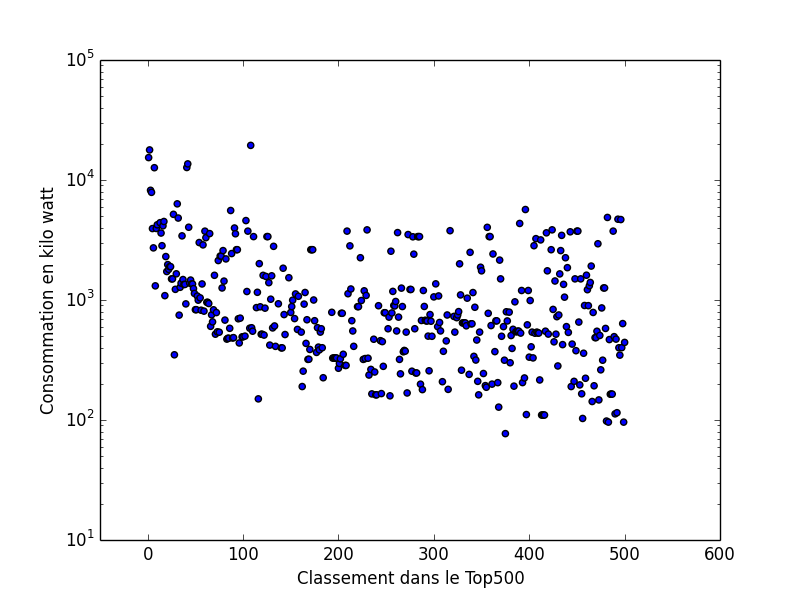
\includegraphics[width=10cm]{images/Chapitre1/pic_top500_power.png}
                    \caption{\label{pic_top500_power} Consommation électrique des 500 supercalculateurs les plus puissants (2018).}
                \end{figure}
      
      
        Le Département de l'énergie des États-Unis (DoE) a publié son rapport de propositions PathForward, et a établi qu'un supercalculateur exaflopique devra consommer au maximum entre 20 et 30 mégawatts \cite{Ang2016}. Actuellement, les quatre premiers supercalculateurs consomment entre 7 et 18 MW. La construction d'une plateforme exascale implique donc de réaliser 30 fois plus d'opérations avec une enveloppe énergétique seulement doublée. L'énergie est une contrainte majeure dans la construction d'une plateforme Exascale. Pour nous en rendre compte, nous étudions le dernier classement du Top500 paru en novembre 2019. Pour obtenir une puissance cumulée d'un exaFLOPS, il faut additionner la puissance des 105 premiers supercalculateurs du Top500. Une telle plateforme nécessiterait alors une alimentation de plusieurs centaines de mégawatts. Le même exercice peut être réalisé avec le classement du Green500 (voir \autoref{tab:green500}), qui classe les architectures les plus efficaces du Top500. Pour obtenir une puissance cumulée d'un exaFLOPS, il faudrait regrouper les 205 premiers supercalculateurs pour obtenir une plateforme consommant 279 MW. Ces rapides calculs permettent de montrer l'étendue vertigineuse des améliorations qui sont nécessaires pour la construction d'une plateforme qui respecterait les critères de consommation \cite{Ang2016}. 
        
        
        
        \paragraph{Consommation de la microarchitecture.} 
            
            Ajouter des serveurs pour la construction d'un supercalculateur plus puissant nécessite une plus grande puissance électrique. Cette technique est restée viable pendant plus de vingt ans, alors que les processeurs ne consommaient que quelques watts. Aujourd'hui, les processeurs utilisés ont une enveloppe thermique (TDP) dépassant la centaine de watts: 190 watts pour le processeur IBM Power9 22 coeurs (utilisé dans le supercalculateur Summit), 150 watts pour le processeur Intel Skylake 6148 20 coeurs (utilisé dans le 8e supercalculateur du classement du Top500 2019). Les plateformes les plus puissantes associent à un processeur un ou plusieurs accélérateurs (principalement des GPU). Chaque noeud du supercalculateur Summit possède ainsi 2 processeurs et 6 GPU NVidia V100 ayant chacun un TDP de 250 watts. À de telles consommations, il n'est plus viable d'ajouter des noeuds de calculs indéfiniment, que ce soit pour une raison de coût ou bien de faisabilité. En effet, les sites où sont construits les centres de données ont des lignes électriques déjà existantes et qui ne peuvent pas supporter de plus grandes puissances. Une partie des utilisateurs sont donc limités par cette enveloppe énergétique et doivent l'utiliser le plus efficacement pour la transformer en puissance de calcul. La consommation électrique des architectures varie fortement en fonction des opérations réalisées (voir \autoref{fig:energy_pj}). Que ce soit pour des architectures 32 bits \cite{Horowitz2014} ou 64 bits \cite{Leland2014} la consommation électrique des opérations élémentaires de la microarchitecture n’a que très peu évolué ces dernières années. Nous constatons que la majorité du budget énergétique est allouée au déplacement des données entre la mémoire et les caches. Il est donc primordial d'apporter des solutions matérielles et logicielles permettant de réduire la consommation de ces opérations.
        
            \begin{figure}
            \center
            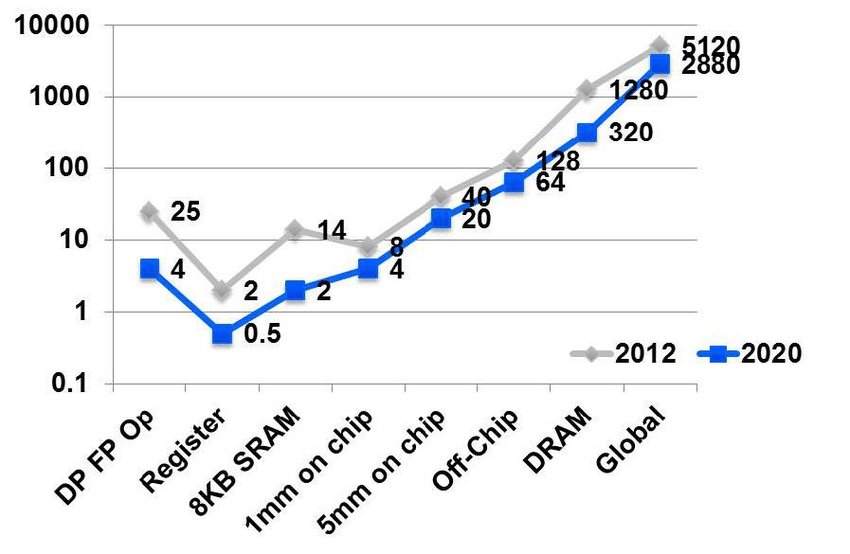
\includegraphics[width=10cm]{images/energy_pj.png}
            \caption{\label{fig:energy_pj} Coût énergétique, en picojoules (pJ) par opération à virgule flottante de 64 bits, pour diverses opérations courantes dans un ordinateur. La ligne supérieure (grise) représente le coût énergétique des opérations sur un processeur utilisé en 2012. La ligne inférieure (bleue) prévoit les coûts énergétiques en 2020 \cite{Leland2014}.}
            \end{figure}
            
                

        
        \paragraph{Le cas du supercalculateur Summit.} 
        
            Pour étudier la contrainte énergétique dans l'élaboration d'une plateforme Exascale, nous étudions certaines caractéristiques du supercalculateur Summit présentées dans le \autoref{tab:summit_analysis}. Ce dernier est classé numéro un au Top500 de novembre 2019 (voir \autoref{sec:Top500}). Il est aussi le premier supercalculateur du classement du Green500 consommant plus de 10 MW  (classé 5e en novembre 2019). Pour appréhender l'importance des efforts à fournir pour construire un supercalculateur capable d'exécuter $10^{18}$ opérations par seconde pour une application réelle, nous comparons l'efficacité énergétique de Summit avec celle d'un supercalculateur Exascale pour l'exécution du benchmark HPL.
        
            \begin{table}[]
            \centering
            \resizebox{\textwidth}{!}{%
            \begin{tabular}{|l|c|c|c|c|c|}
            \hline
            \rowcolor[HTML]{EFEFEF} 
            \textbf{Supercalculateur} & \textbf{\begin{tabular}[c]{@{}c@{}}Consommation\\ (MW)\end{tabular}} & \textbf{\begin{tabular}[c]{@{}c@{}}Perf. Linpack\\ (exaFLOPS)\end{tabular}} & \textbf{\begin{tabular}[c]{@{}c@{}}Efficacité énergétique\\ (GFLOP/watt)\end{tabular}} & \textbf{\begin{tabular}[c]{@{}c@{}}Budget énergétique\\ (pJ/opération)\end{tabular}} & \textbf{\begin{tabular}[c]{@{}c@{}}Conso. Linpack\\ (pJ/bit)\end{tabular}} \\ \hline
            \cellcolor[HTML]{EFEFEF}\textbf{Summit} & 10 & 0.200 & 20 & 50 & 0.25 \\ \hline
            \cellcolor[HTML]{EFEFEF}\textbf{Projet Exascale} & 20 - 30 & 1 & 50 - 33 & 20 - 30 & 0.1 - 0.15 \\ \hline
            \end{tabular}%
            }
            \caption{Comparaison de l'efficacité énergétique du supercalculateur Summit et de l'efficacité théorique d'une plateforme exascale\textbackslash{}cite\{Bergman2018\}.}
            \label{tab:summit_analysis}
            \end{table}
    
    
            Pour fonctionner, Summit a besoin d'une puissance de 10 MW. En novembre 2019, il a atteint une performance de 200 pétaFLOPS ($10^{15}$ \gls{FLOPS}) lors de l'exécution du benchmark Linpack. Son efficacité énergétique est donc de 20 GFLOP/watt. Un supercalculateur exaflopique consommant entre 20 et 30 MW aurait quant à lui, une efficacité énergétique comprise entre 33 et 50 GFLOP/watt. Le challenge est donc de construire une plateforme 5 fois plus puissante tout en étant deux fois plus efficace énergétiquement. Cependant, le défaut du benchmark Linpack est qu'il ne reflète pas le comportement des applications industrielles. En effet, contrairement aux applications réelles, il ne nécessite aucune communication entre les noeuds, et les instructions sont réalisées sur des données présentes dans le cache. Atteindre un exaFLOPS sur le benchmark HPL sera bien plus facile que d'atteindre la même performance avec une application réelle dont la consommation est principalement due aux déplacements mémoires. Pour mieux appréhender l'impact énergétique des déplacements mémoires, nous calculons l'efficacité énergétique des deux supercalculateurs étudiés en joule/FLOP:
            \begin{equation}
                 \frac{FLOPS}{watt}  =  \frac{\frac{FLOP}{seconde}}  { \frac{joule}{second}} =  \frac{FLOP}{joule}
            \end{equation}
            Nous calculons ainsi le \textit{budget} disponible pour exécuter une opération flottante: 50 pJ pour Summit, contre 20 pJ et 30 pJ pour le supercalculateur Exascale. En moyenne, l'application exécute des instructions vectorielles de 200 bits \footnote{Source - \url{https://insidehpc.com/2019/07/flexibly-scalable-high-performance-architectures-with-embedded-photonics/}}. L'énergie dépensée par Summit pour calculer un bit est alors de 0.25 pJ. Pour une plateforme exascale, ce budget énergétique serait alors compris en 0.1 et 0.15 pJ/bit.
            
            Un accès à la mémoire se compte en centaine de picojoules par bit et en millier lorsqu'il s'agit de communication entre deux noeuds de calculs. Lorsque l'énergie disponible est de 0.1 pJ/bit et qu'un accès mémoire peut dépasser de cent fois ce budget, il est facile de comprendre que l'essentiel des innovations doivent se porter sur l'amélioration des communications (à l'intérieur des serveurs, mais aussi à l'extérieur) que ce soit par l'utilisation de nouvelles technologies ou d'une restructuration des microarchitectures. Les applications et les algorithmes doivent eux optimiser l'utilisation des données locales pour tirer profit des principes de localité (voir \autoref{sec:locality}).


    \subsubsection{La complexité}\label{sec:edl_chal_complexite}
    %%%%%%%%%%%%%%%%%%%%%%%%%%%%%%%%%%%%%%%%%%%%%%%%%%%%%%%%%%%%%%%%%%%%%%%%
    %%%%%%%%%%%%%%%%%%%%%%%%%%%%%%%%%%%%%%%%%%%%%%%%%%%%%%%%%%%%%%%%%%%%%%%%
        
        Comme présenté dans l'\aref{chap:sota:materiel}, les architectures des ordinateurs ont reçu de nombreuses améliorations au fil des ans. Ces améliorations se sont additionnées et ont permit le développement des processeurs tels que nous les connaissons aujourd'hui: une hiérarchie mémoire, plusieurs coeurs (logique et physique), un pipeline comportant souvent plus de dix étapes, des systèmes d'exécution dans le désordre ou encore de préchargement mémoire. 
        
        La complexification est aussi présente dans le logiciel. Pour tirer parti des fonctionnalités offertes par le matériel, plusieurs modèles de programmation sont utilisés pour par exemple exploiter la mémoire partagée et distribuée ou utiliser les différents coeurs d'un processeur. En fonction des tâches à réaliser, plusieurs langages peuvent être utilisés dans une même application (C, C++, fortran, python, cuda...). La programmation \textbf{efficace} d'un supercalculateur est ainsi devenue une tâche très difficile. La complexification du matériel et du logiciel a un fort impact sur la performance des applications qui parviennent rarement à exploiter une part significative de la performance disponible. La performance d’une même application peut fortement varier à cause d’une subtilité (la configuration du BIOS, un réglage du système d’exploitation). Certaines technologies (FPGA, GPU) ne sont pas envisagées par des entreprises, car l'adaptation de leurs applications pour fonctionner sur celles-ci est très difficile. Pour s'extraire de la complexité grandissante des plateformes HPC et de leur gestion, de plus en plus d'utilisateurs se tournent vers des solutions dématérialisées telles que le \textit{cloud}.
        
        %Dans le classement du Top500, on remarque ainsi que les supercalculateurs atteignent rarement plus de 80\% d'efficacité sur une application simple comme Linpack\cite{Dongarra2003}. Pour des applications réelles, cette efficacité est encore plus faible, parfois inférieure à 10\%\cite{Oliker2005}. 
        %La complexité des architectures a aussi un impact sur l'efficacité énergétique des plateformes, par exemple le mécanisme de prédiction de branchement ou l'agrandissement des différents niveaux du \textit{pipeline} (voir \autoref{sec:pipeline}).
        
        \paragraph{La sécurité.} La complexité du matériel et des couches logicielles représente un grand risque d'exploitation de faille de sécurité. Les applications utilisent de nombreuses librairies qui peuvent présenter des failles, et la difficulté de les mettre à jour (pour la stabilité des applications) peut permettre aux attaquants d'exploiter ces failles. L'accumulation de fonctionnalités a aussi rendu ces architectures sujettes à différentes attaques. En 2018, les chercheurs de Google \cite{kocher2018spectre} ont découvert une faille majeure dans le prédicteur de branchement des processeurs Intel (voir \autoref{sec:micro}). Aujourd'hui, les supercalculateurs sont rarement directement connectés au réseau internet, rendant difficile l'attaque de ces plateformes. Cependant, la vision exascale présentée dans le début du chapitre implique la collecte de données et le traitement des données au plus proche de la source de leur création ainsi que l'acheminement de certains résultats vers les centres de calculs, exposant de nombreux lieux d'attaque. Il n’est pas envisageable d'utiliser des voitures autonomes possédant des processeurs, des mémoires, des dizaines de couches logiciels pouvant être attaqués. De même, les données personnelles, tels que les données médicales enregistrées par les montres connectées sont très sensibles.
    
        
        \paragraph{Passage à l'échelle.} Pour obtenir un supercalculateur exascale, il est techniquement possible de construire 5 supercalculateurs de la puissance du Summit et d’agréger leur performance. Cependant, pour les raisons de coût, principalement lié à la consommation énergétique, cette solution n’est pas envisageable. À une telle échelle, le nombre de serveurs serait si important (supérieur à 30000) que des problèmes insoupçonnés à des tailles moindres feraient leur apparition. Les pannes des matériels, les congestions de réseaux et la capacité des applications à utiliser un grand nombre de serveurs impacteraient leur performance rendant le supercalculateur très inefficace. En effet, la programmation parallèle nécessite la synchronisation des ressources à différentes étapes du calculs pour partager des résultats intermédiaires. Ainsi, les pannes matériel d'une seule ressource de calcul ont de forts impacts sur la performance des applications de calculs parallèles. 
        %Ces infrastructures seront utilisées pour exécuter des applications pendant plusieurs heures ou mêmes jours. Il est donc nécessaire de développer des systèmes de reprises suite à une erreur sans avoir à tout recommencer \cite{farjallah2014preparing} grâce à des mécanismes de point de contrôle (\textit{checkpoint}) \cite{Zheng2012}
        

    \subsubsection{Les nouvelles technologies}\label{sec:edl_chal_new_techno}
    %%%%%%%%%%%%%%%%%%%%%%%%%%%%%%%%%%%%%%%%%%%%%%%%%%%%%%%%%%%%%%%%%%%%%%%%    %%%%%%%%%%%%%%%%%%%%%%%%%%%%%%%%%%%%%%%%%%%%%%%%%%%%%%%%%%%%%%%%%%%%%%%%

        Nous avons montré précédemment que les utilisateurs étaient en demande de puissance de calcul supplémentaires. 
        Le classement du Top500,  réalisé tous les 6 mois, permet de classer les plateformes les plus récentes. Les nombreux supercalculateurs construits chaque année rentrent au classement, remplaçant les anciennes plateformes moins performantes. Sur la \autoref{fig:edl_top500_age}, nous constatons que l'âge moyen du Top500 a doublé en quelques années indiquant la difficulté à produire des supercalculateurs plus performantes. Alors que l'âge moyen du classement oscillait autour de 7 mois pour les 23 premières années du classement, il a dépassé les 15 mois depuis les années 2013. Ces deux constats montrent que les utilisateurs de HPC ne renouvellent plus leurs supercalculateurs, car ils ne trouvent plus de solutions matérielles suffisamment intéressantes pour motiver de nouveaux investissements. De nouvelles technologies doivent émerger pour obtenir de réels gains de performance. L'histoire récente nous a prouvé que ce chemin était le bon à suivre avec l'utilisation des GPU (ou d'accélérateurs dédiés comme les TPU de Google) pour accélérer les applications d'apprentissage par machine. Les pressions économique et énergétique présentées précédemment nous indiquent que de nombreuses avancées doivent être réalisées dans tous les domaines touchant au HPC: les processeurs, les accélérateurs, les mémoires, les réseaux ou bien la partie logiciel. 
        
        
                  
            \begin{figure}
                \center
                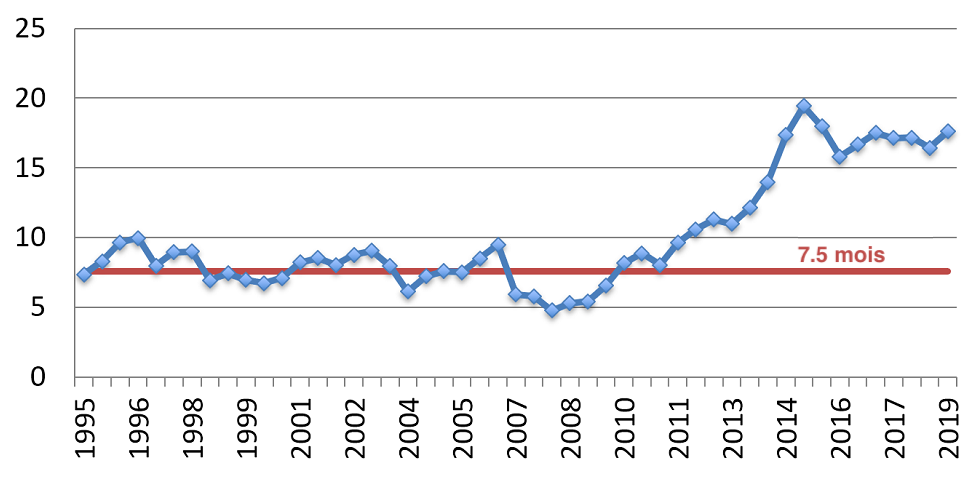
\includegraphics[width=10cm]{images/edl_top500_age.png}
                \caption{\label{fig:edl_top500_age} Âge moyen des supercalculateurs classés au Top500 \cite{Strohmaier2018}.}
            \end{figure}
       
        %Exemple de nouveauté
        

        \paragraph[Explosion cambrienne] {Explosion ``cambrienne'' \footnote{L’explosion cambrienne désigne l'apparition soudaine (à l'échelle des temps géologiques) de la plupart des grands embranchements actuels des animaux pluricellulaires ainsi qu'une grande diversification des espèces animales, végétales et bactériennes (wikipédia).}}
        
            De nouvelles technologies existent ou sont en cours de développement. Dans la \autoref{sec:oppo_new_tech}, nous montrons que de nombreuses solutions matérielles, technologiques et logiciels peuvent être utilisées. Des accélérateurs et des mémoires très spécifiques pourront être utilisés. Les utilisateurs de HPC et les architectes doivent alors connaître les besoins de leurs applications pour choisir quelles technologies utiliser (type et quantité de mémoire, utilisation d'accélérateurs). Si ces nouvelles technologies peuvent être une réelle opportunité pour l'élaboration de plateformes plus puissantes et plus efficaces, elles sont aussi un challenge. En effet, jusqu’à récemment, la majorité des plateformes étaient construites de façon similaire: un processeur x86 pouvant être associé à un GPU (voir \autoref{sec:edl_hpc_hetero}). Si les applications obtenaient de faibles performances, il était difficile de s'orienter vers d'autres solutions alors inexistantes. La majorité des supercalculateurs sont utilisés par différents utilisateurs et exécutent différents types d'applications. Le choix des technologies utilisées doit alors prendre en compte ces différentes applications pour construire la plateforme la plus efficace possible. Souvent ces centres de calculs seront hétérogènes avec différents processeurs.
        
        \paragraph{Nouveautés au Top500.} En étudiant le classement du Top500, nous constatons les premiers signes de l'évolution des plateformes qui utilisent de nouveaux types de processeurs ou d'accélérateurs (voir \autoref{fig:new_proc}). En novembre 2019, trois supercalculateurs classés à la 84e, 72e et 116e place étaient équipés de processeur Sparc64 XIfx \cite{Yoshida2018}. Ce processeur est produit par Fujitsu et possède 34 coeurs (dont deux réservés en priorité au système d'exploitation et à la gestion des communications). Il possède 24 Mb de cache L2 et atteint une performance de 1,1 téraFLOPS (voir \autoref{fig:edl_sparc64}). Pour atteindre de hautes performances sur des applications réelles, le processeur est doté d'une mémoire empilée HMC de 32 GB \cite{Garg2017}. Concernant les accélérateurs, nous pouvons citer le coprocesseur Matrix-2000 qui a permis de doubler la puissance du supercalculateur chinois Tianhe-2 en remplaçant les anciens accélérateurs KNL par une nouvelle architecture développée exclusivement pour lui. Cet accélérateur 64 bits produit par NUDT, possède 128 coeurs RISC à 1,2 GHz permettant d'atteindre une performance crête de 4,92 téraFLOPS pour une enveloppe thermique de 240W. Quatre groupes de 32 coeurs sont reliés à la mémoire avec un total de 8 canaux mémoires (voir \autoref{fig:edlp_matrix_2000}). 
        
          
        \begin{figure}[t!]
            \centering
            \begin{subfigure}[t]{0.48\textwidth}
                \centering
                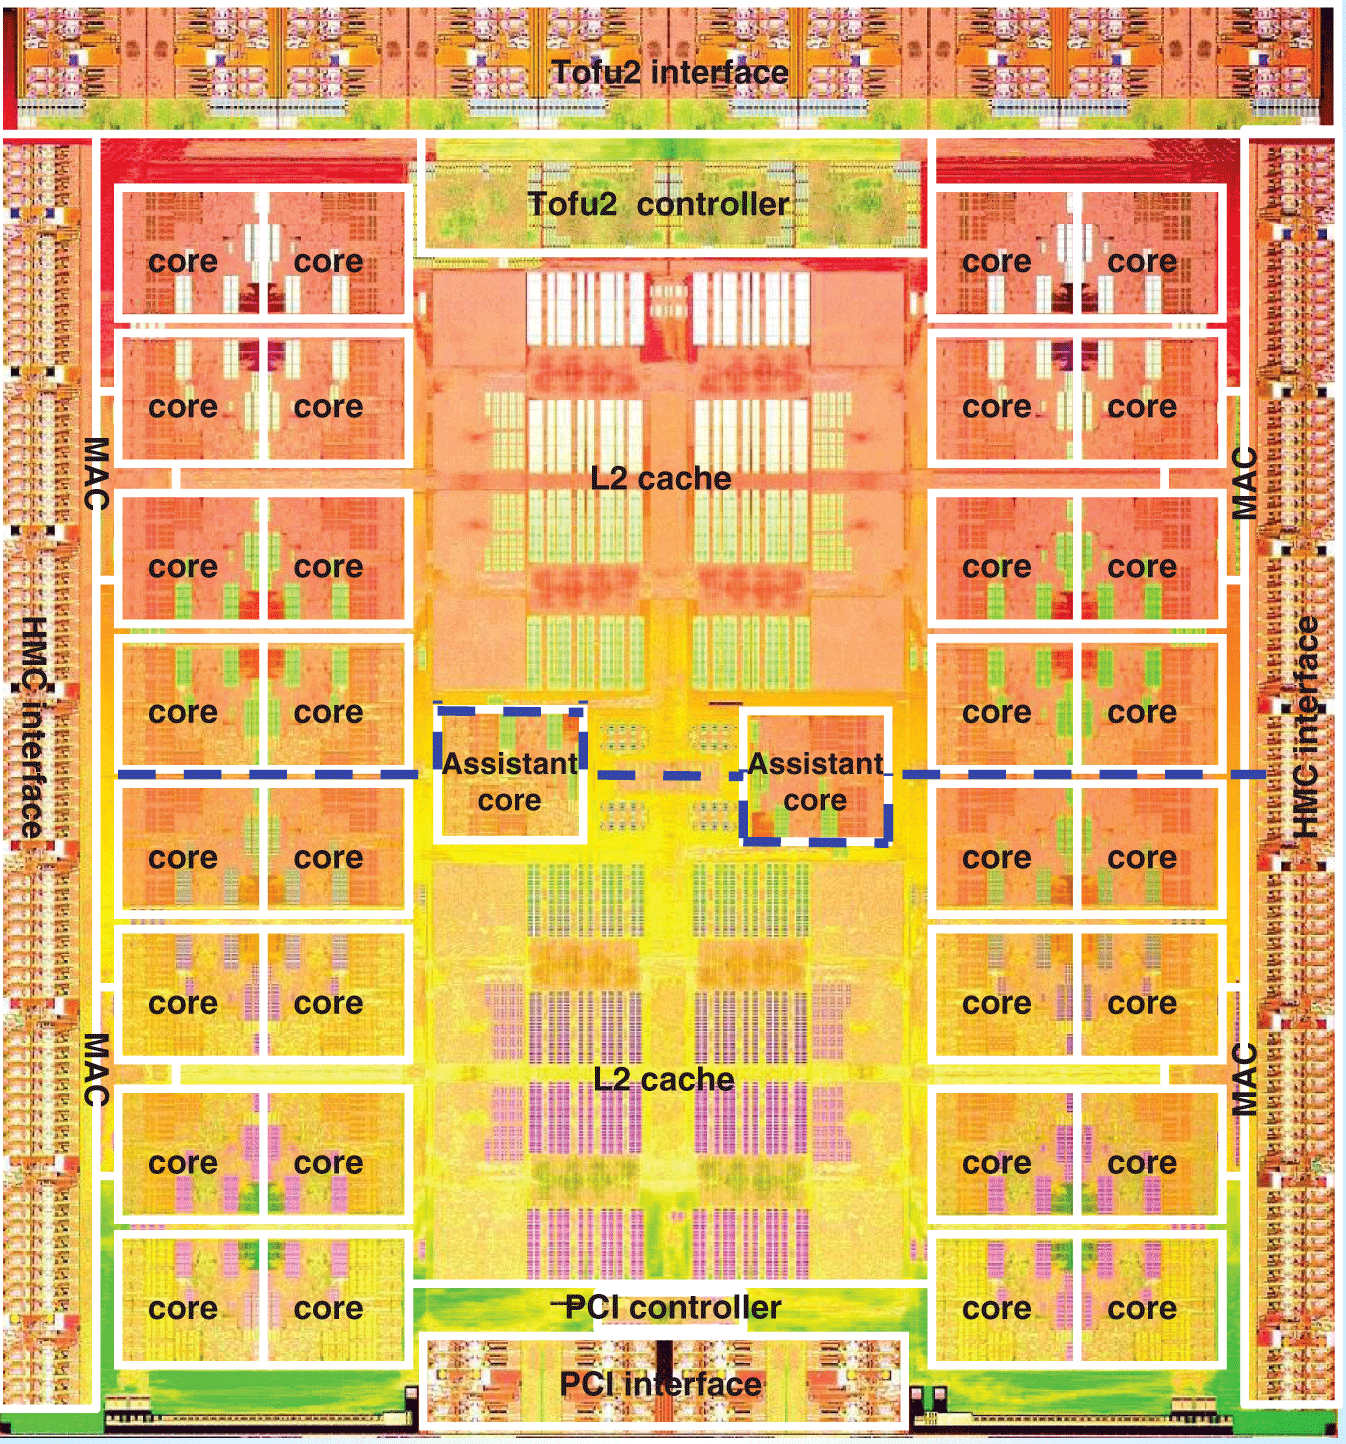
\includegraphics[width=0.9\linewidth]{images/edl_sparc64.png}
                \caption{\label{fig:edl_sparc64} Le processeur Sparc64 est produit par Fujitsu et utilise une mémoire empilée HMC\cite{7021857}.}
            \end{subfigure}\hfill
            \begin{subfigure}[t]{0.48\textwidth}
                \centering
                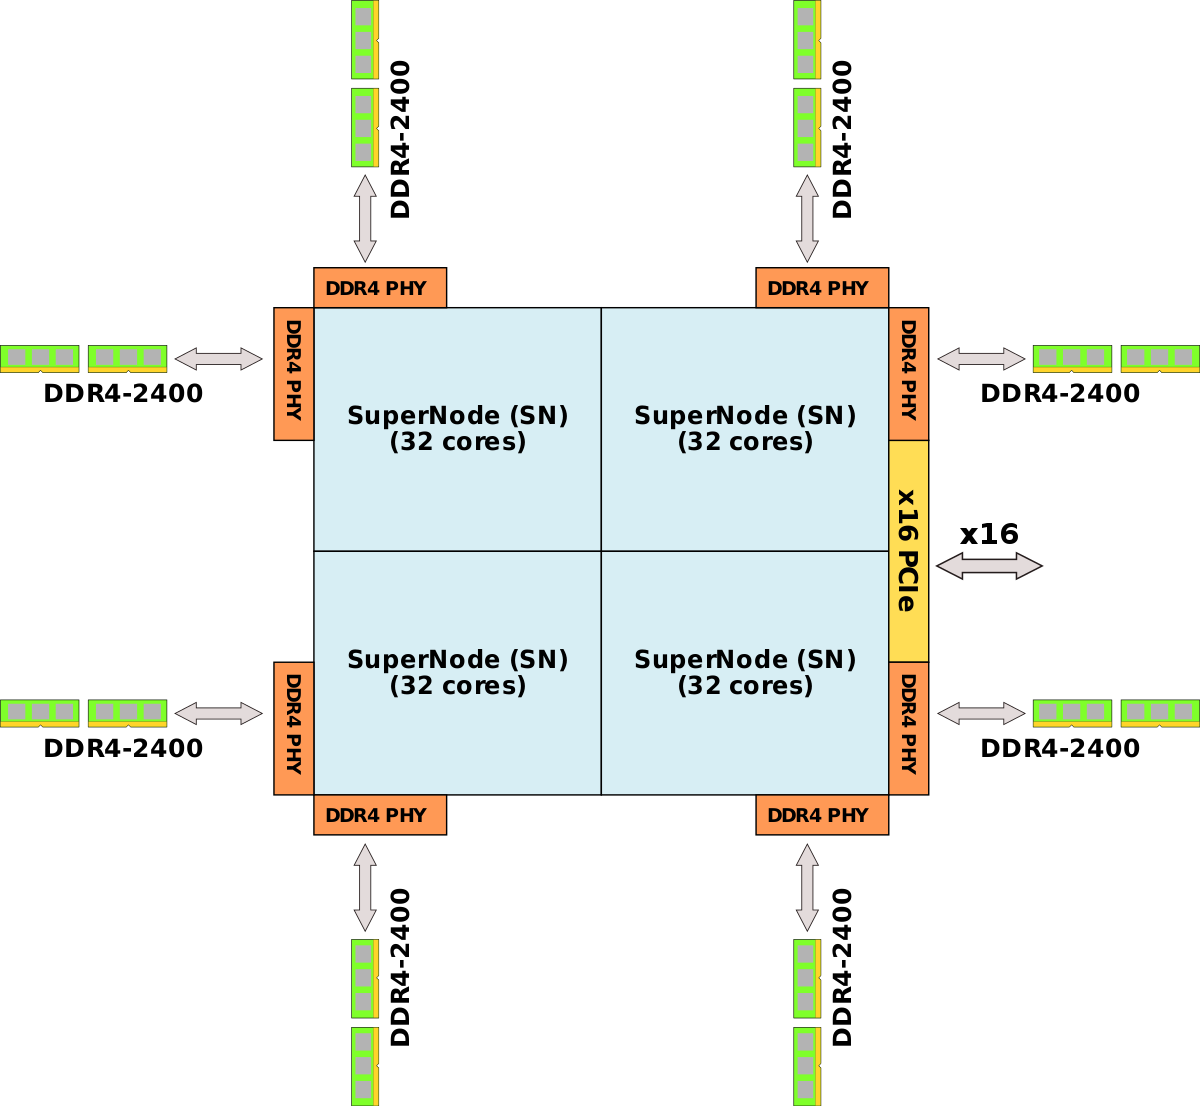
\includegraphics[width=\linewidth]{images/edlp_matrix_2000.png}
                \caption{\label{fig:edlp_matrix_2000}Le coprocesseur Matrix 2000 possède 128 coeurs et 8 canaux mémoires.}
            \end{subfigure}
            \caption{\label{fig:new_proc} De nouvelles architectures sont utilisées dans les supercalculateurs classés au Top500.}
        \end{figure}

           
    \subsubsection{Rapidité de l'évaluation des nouvelles technologies} \label{sec:edl_chal_vitesse}
    %%%%%%%%%%%%%%%%%%%%%%%%%%%%%%%%%%%%%%%%%%%%%%%%%%%%%%%%%%%%%%%%%%%%%%%%    %%%%%%%%%%%%%%%%%%%%%%%%%%%%%%%%%%%%%%%%%%%%%%%%%%%%%%%%%%%%%%%%%%%%%%%%
        
        Face à l'arrivée de ces nombreuses technologies, les entreprises doivent rapidement être capables d'évaluer leurs qualités et leurs défauts et quantifier leur adéquation avec leurs applications. Les évolutions récentes sont très rapides avec le développement de dizaines de modèles de mémoire, de nouveaux accélérateurs et de processeurs. Certaines technologies encore en développement sont déjà dépassées par l’annonce de nouvelles technologies.
        
        Une technologie émergente, très performante pour une application, avec des consommations énergétiques ou un coût très faible peut permettre à une industrie de faire un bond de performances dans un domaine. Grâce à ces technologies, l'économie d'un domaine peut être fortement modifiée en permettant de réaliser des simulations dix fois plus rapidement ou en divisant leur coût du même facteur.
                
        La vitesse de décision et d'utilisation d'une nouvelle technologie dans notre société mondialisée est cruciale. Les entreprises doivent donc disposer de moyens (technique et financier) pour se tenir à l'état de l'art des technologies. Le développement de partenariat (avec des universités par exemple) est une des clefs permettant de s’assurer de la capacité des entreprises à ingérer ces nouvelles technologies.


    \subsubsection{L'expertise}\label{sec:edl_chal_expertise}
    %%%%%%%%%%%%%%%%%%%%%%%%%%%%%%%%%%%%%%%%%%%%%%%%%%%%%%%%%%%%%%%%%%%%%%%
    %%%%%%%%%%%%%%%%%%%%%%%%%%%%%%%%%%%%%%%%%%%%%%%%%%%%%%%%%%%%%%%%%%%%%%%%

        Pour construire les plateformes de demain, il est nécessaire de pouvoir qualifier les nouvelles architectures émergentes. Cette qualification devant se faire rapidement sur des dizaines d'architectures différentes, il est important pour les acteurs du HPC d'avoir les moyens adéquats pour réaliser cette mission. Pour motiver les choix réalisés, une modélisation économique des performances ($FLOP/\$$, $GB/s/\$$) doit pouvoir être réalisée. Une fois les architectures sélectionnées, les programmeurs doivent être capables d'extraire une part importante des performances disponibles. Les architectures ciblées pouvant être très différentes des processeurs x86 largement utilisés aujourd'hui, les programmeurs doivent avoir de solides connaissances et les outils adaptés, sans quoi certaines architectures devront être abandonnées. Les outils à leur disposition doivent leur permettre d'établir un profil des besoins de son application pour pouvoir caractériser et sélectionner les différentes plateformes. Pour étudier son application et valider leur performance une fois le code porté, il est nécessaire d'avoir des outils facilement utilisables sur différentes plateformes (et différentes microarchitectures).
        
        Les FPGA (Field Programmable Gate Array) en sont un bon exemple. Cette technologie permet de faire des périphériques très performants et très efficaces en termes de consommation électrique. L'idée principale étant de laisser au programmeur le développement complet du circuit électronique pour qu'il corresponde parfaitement à son besoin. Mais la programmation de tels circuits est très complexe et demande des mois, souvent des années pour des codes industriels, pour être réalisée. Ainsi, malgré l'efficacité, prouvée, de cette technologie, les entreprises ne s'y lancent pas à cause des coûts engendrés par l'achat du matériel et la taille des équipes requises pour programmer et supporter les applications. 
        
        
        %\paragraph{Programmation des supercalculateurs.} Dans la \autoref{sec:edl_chal_complexite} nous avons rappelé la complexité de programmer un supercalculateur, qui nécessite l'utilisation de plusieurs modèles de programmation et souvent de plusieurs langages. L'apparition de plateforme hétérogène (voir \autoref{sec:edl_hpc_hetero}) va rendre la tâche d'autant plus difficile. Pour l'aider, le programmeur doit avoir à sa disposition une couche logicielle et un modèle de programmation pour l’aider, lui permettant de se concentrer seulement sur le développement de son algorithme. Les outils de répartition de charges doivent être améliorés pour prendre en compte l'hétérogénéité des architectures disponible.
        
        
        \paragraph{Optimisations des codes.} 
            
            Le challenge de l’exascale ne vient pas seulement du matériel et des technologies que nous allons utiliser comme le soulignent certains travaux \cite{barrett2012navigating}. Il  nécessite aussi de repenser une grande partie des logiciels. Cette partie est très délicate, car les applications atteignent souvent plusieurs dizaines de milliers de lignes de codes. Changer un compilateur ou un debugger peut alors s’avérer plus complexe qu'il n’y parait. Pour atteindre les meilleures performances possible, les programmeurs doivent être capables d'écrire des applications optimisées pour les architectures utilisées. Pour cela, il est nécessaire de restructurer le code ou d'utiliser d'autres algorithmes pour tirer parti des caractéristiques du matériel (hiérarchie de cache, taille de la mémoire, nombre de coeurs...). Des optimisations telles que le découpage en bloc \cite{Xue2012} ou le \textit{time squewing} \cite{Wonnacott2002} existent et ont prouvé leur efficacité. Cependant, leur implémentation sur des applications industrielles peut être très fastidieuse et les performances atteintes peuvent être différentes de celles attendues. 
            
            %Cette partie pourrait être laissée au compilateur, mais il est très difficile de proposer un tel compilateur générique étant capable de les implémenter. Les compilateurs ont un rôle central dans le développement et l’exécution des applications, car ils sont l’intermédiaire entre le programmeur et le matériel. Leur efficacité à générer du code de qualité est primordiale pour tirer le maximum de performances de ces architectures complexes.

        %Algo
        \paragraph{Adapter les algorithmes.} Une source (presque) inépuisable d'accélération des applications vient de l'utilisation de nouveaux algorithmes. La \autoref{fig:edl_new_algo}, montre comment l'utilisation de nouvelles méthodes mathématiques permet d'accélérer de plusieurs facteurs la résolution d'une équation de poisson. Une application nécessitant 6 mois de calculs en 1947 peut être résolue grâce à une méthode multi grille \cite{Brandt1982} en moins d'une seconde.
            
            Pour réduire le nombre d’opérations lors de la multiplication de matrices pour les algorithmes d’apprentissage par machine, plusieurs techniques peuvent être utilisées \cite{Sze2017}: la transformée de Fourier rapide \cite{Vasilache2014}, l’algorithme de Strassen \cite{Cong2014} ou encore l'algorithme de Coppersmith-Winograd \cite{Li2016}. En fonction des caractéristiques de l’architecture (stockage disponible), du besoin de stabilité numérique, ou de la taille des matrices utilisées, chaque méthode à ses avantages et inconvénients. Le compilateur peut alors choisir la meilleure technique à utiliser en fonction de ces paramètres.
    
            \begin{figure}
            \center
            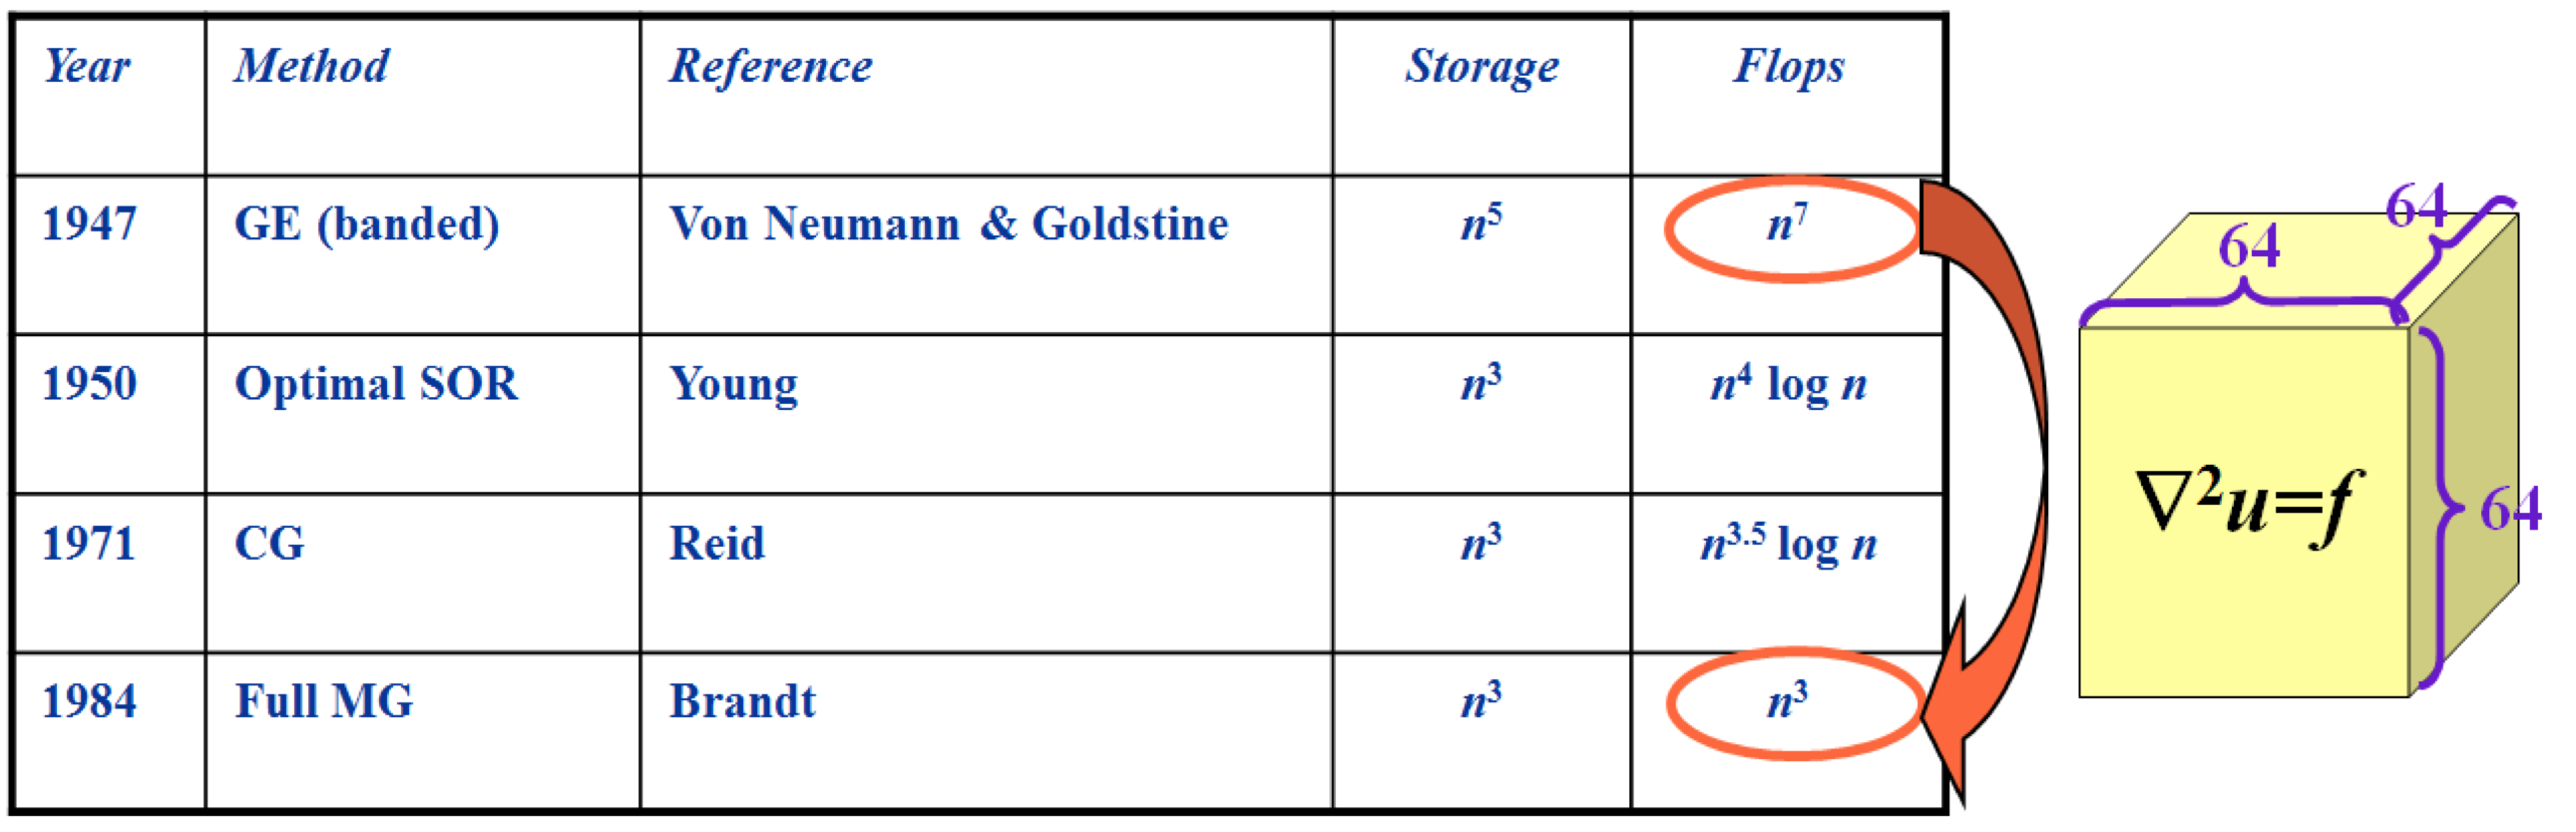
\includegraphics[width=14cm]{images/edl_new_algo.png}
            \caption{\label{fig:edl_new_algo} L'utilisation de nouvelle méthodes mathématique à permis de réduire de plusieurs facteurs la quantité de stockage (\textit{storage}) et le nombre de calculs nécessaires (\textit{flops}) pour la résolution d'une équation de poisson\protect\footnotemark.}
            \end{figure}
            \footnotetext{Tableau extrait de la présentation de David Keyes - \url{http://www.cs.odu.edu/~keyes/talks/SC_IMI.ppt}}

            Pour les plateformes exascale, les algorithmes doivent être adaptés à certaines contraintes. Le coût des déplacements des données, en énergie et en temps, doit être le moteur de leur développement et de leurs améliorations. En effet, le coût énergétique de l'exécution d’une opération flottante peut être considéré comme gratuit quand on le compare au coût du déplacement des données. La plus grande pénalité venant des communications entre les noeuds de calculs, les algorithmes doivent réduire au maximum ces communications en découpant stratégiquement le jeu de données. Il peut même être avantageux de recalculer certains résultats localement, plutôt que de les communiquer entre deux serveurs. L'algorithme de Strassen \cite{Lipshitz2012} permet par exemple la multiplication de deux matrices sans échanges de données. Ces techniques ont un gain double: elles sont plus rapides, car l’exécution n’est pas pénalisée par la performance du réseau, et elles sont plus efficaces énergétiquement, car elles ne payent pas le coût de la communication des données. Cependant, ces méthodes peuvent entraîner des problèmes de stabilité numérique \cite{khabou2013dense}. 
                        

        \paragraph{Challenge.}  
        
            La complexification des applications et du matériel confronté au manque de connaissances et d'outils des utilisateurs se traduit par une mauvaise utilisation des plateformes évoquée dans la \autoref{sec:Top500}. Bien que la recherche ait réalisé de nombreuses découvertes, peu d'entre elles sont réellement appliquées sur les codes industriels. La loi de Moore assurant une évolution constante des performances des architectures, l’analyse et l’optimisation des codes ont été laissées de côté. Les investissements réalisés dans le développement des matériels se sont faits au détriment des logiciels. Aujourd'hui, nous constatons un manque de connaissances fines des architectures dû à leur complexité croissante ainsi que le manque d'outils adéquats pour réaliser les optimisations nécessaires.
        

\section{Opportunités}\label{sec:oppo}
%%%%%%%%%%%%%%%%%%%%%%%%%%%%%%%%%%%%%%%%%%%%%%%%%%%%%%%%%%%%%%%%%%%%%%%%
    
    %Fin d'un modèle
    Nous avons montré dans les sections précédentes que poursuivre la stratégie qui consistait à ajouter toujours plus de serveurs pour construire un supercalculateur, n'est plus viable. Nous avons présenté les principaux défis que les utilisateurs de HPC doivent relever et les barrières rencontrées. Pour y parvenir, des évolutions technologiques majeures doivent être faites et l'architecture des plateformes doit être repensée.
    Ce constat est partagé par les auteurs du rapport de Pathforward \cite{Lucas2014}: ``\textit{Les améliorations considérables nécessaires à la réalisation d'un supercalculateur \gls{exascale} ne seront pas satisfaites par des améliorations progressives des techniques conventionnelles actuelles.}''
    Si les défis sont nombreux et difficiles à relever, de nombreuses opportunités sont disponibles. Dans cette section, nous présentons les opportunités principales à considérer: l'apparition de nouvelles technologies très différentes de celles actuellement utilisées et la reconsidération complète de l'architecture des plateformes. 


\subsection{Investissements financiers}
%%%%%%%%%%%%%%%%%%%%%%%%%%%%%%%%%%%%%%%%%%%%%

    La première condition pour réaliser les nombreux développements technologiques nécessaires est la présence d'investissements financiers. L'industrie du HPC investit massivement dans le développement de nouvelles technologies pour répondre au besoin de puissances de calcul. Une analyse de marché paru en 2016 montre que le marché du High Performance Computing pèsera 36 milliards de dollars en 2020, alors qu'il en valait 28 en 2015\footnote{\url{http://www.marketsandmarkets.com/Market-Reports/Quantum-High-Performance-Computing-Market-631.html}}.

    Si le développement des plateformes exascales est motivé par son aspect financier pour les industries, la construction du premier supercalculateur exascale est un enjeu politique pour les nations. Comme le fut autrefois la course à l'espace et la conquête de la lune, les nations ont à coeur d’être les premières à obtenir une telle architecture et s’en donnent les moyens. L’obtention d’une telle performance est un symbole qui mettra en lumière les acteurs qui y parviendront en premier (nations, universités, constructeurs).

    \paragraph{Investissements Européens} Dans le classement du TOP500 paru en novembre 2017, aucun des 10 supercalculateurs les plus puissants et seulement 5 des 20 meilleurs supercalculateurs mondiaux sont installés en Europe. Alors que l'Asie et l'Amérique se partagent près de 80\% de la puissance de calcul mondiale, l’Europe n'en possède que  18.8\% sur son territoire (voir \autoref{fig:edl_top500_continent}).
    
    \begin{figure}
        \center
        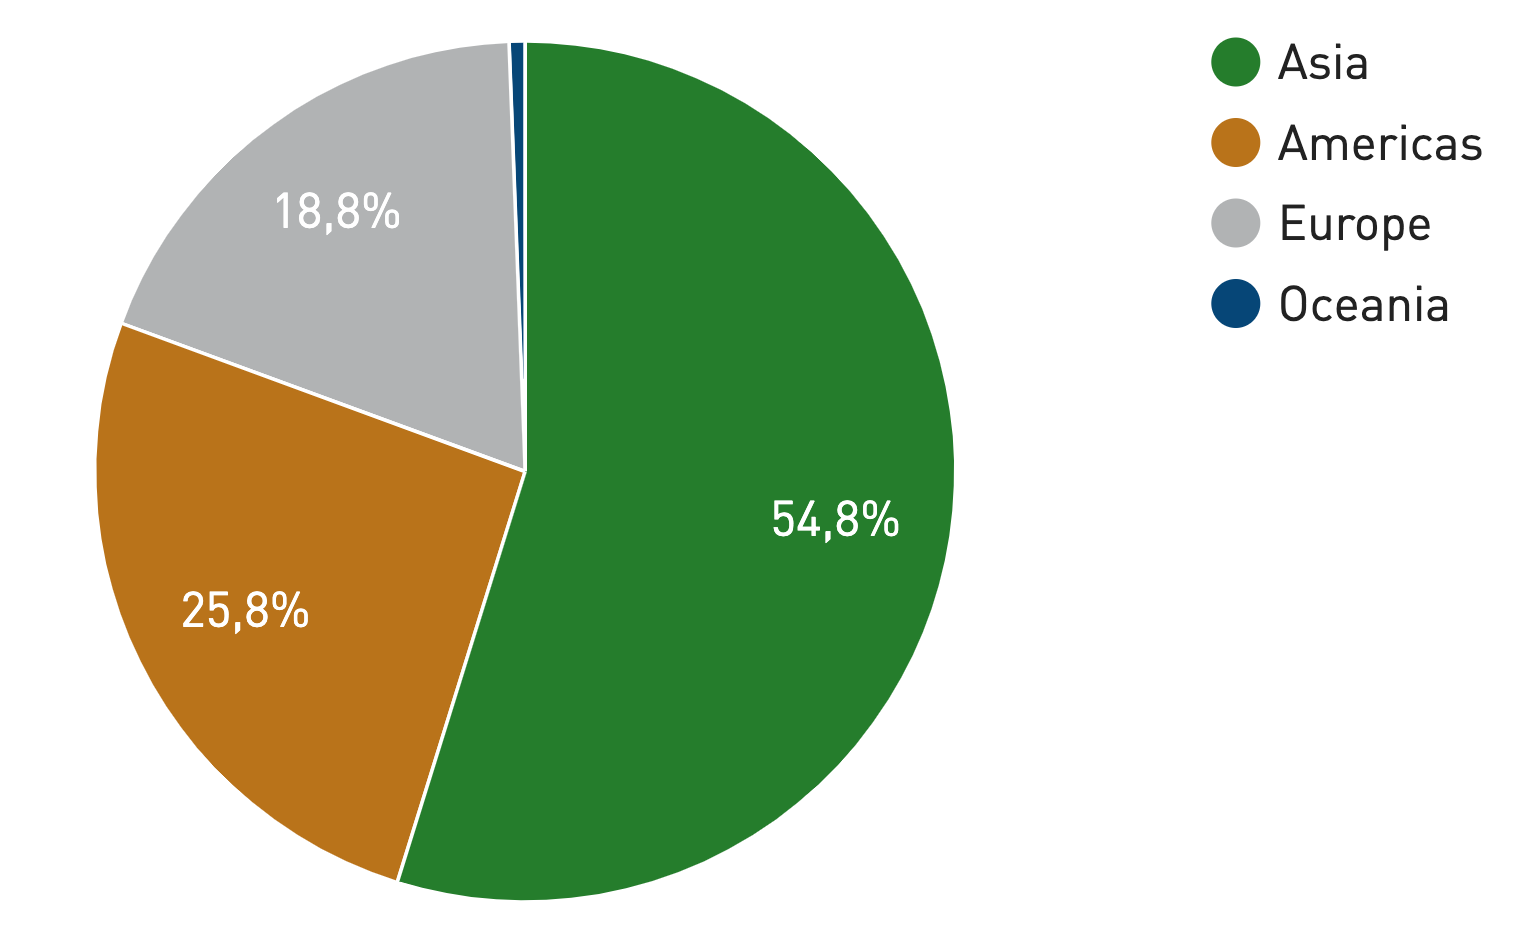
\includegraphics[width=10cm]{images/edl_top500_continent.png}
        \caption{\label{fig:edl_top500_continent} Répartition de la puissance de calcul du Top500 de novembre 2019 entre les continents.}
    \end{figure}
    
    
    Pour accélérer le développement de ses infrastructures, l’Europe a financé un grand projet nommé Horizon 2020. Horizon 2020 est le plus grand programme de recherche et d'innovation jamais mis en place par l'Union européenne. Ce projet d’envergure prévoit d’investir 79 milliards d’euros de 2014 à 2020 pour développer trois piliers : l'excellence scientifique, la primauté industrielle et les défis sociétaux.
    En janvier 2018, la Commission européenne a annoncé investir 1 milliard dans un partenariat réalisé entre le domaine public et privé nommé EuroHPC \cite{EuroHPC2018}. Les objectifs d'EuroHPC sont de développer et déployer une infrastructure de calcul de classe mondiale. 
    Cette entreprise communautaire aura pour objectif de construire 6 supercalculateurs: 2 supercalculateurs petascale ($10^{16}$ opérations) et deux infrastructures ``\textit{pré exascale}'' en 2021. Les architectures pré exascale vont permettre d'utiliser les premières versions des processeurs développées par EuroHPC. Pour assurer son indépendance technologique, le projet EPI (\textit{European Processor Initiative}) a pour objectif de développer de nouveaux processeurs et des accélérateurs MPPA (\textit{massively parallel processor array}) produits par Kalray à Grenoble (voir \autoref{fig:edl_epi_processor}). Enfin, le supercalculateur exaflopique européen prévu entre 2022 et 2023 pourra compter sur de nouvelles architectures, très efficaces énergétiquement, basées sur des processeurs ARM actuellement en développement. Une des motivations étant de réduire sa dépendance aux autres pays pour être plus compétitif.  

    \begin{figure}
        \center
        \includegraphics[width=14cm]{images/edl_epi_processor.png}
        \caption{\label{fig:edl_epi_processor} Les processeurs GPP utiliseront un réseau à mailles 2D sur la puce permettant de relier différents types de coeurs: ARM-V, FPGA embarqué (eFPGA) pouvant être reprogrammé, un processeur vectoriel (MPPA).}
    \end{figure}
    
    
    \paragraph{Les États-Unis.}
    En 2017, le département de l'énergie américain a annoncé le financement d'un projet de 232 millions d'euros nommé PathForward. Ce budget est réparti entre 6 entreprises américaines (HPE, AMD, Cray, IBM, Intel et Nvidia) qui doivent ajouter 40\% de financement supplémentaire pour un total de plus de 400 millions d'euros. L'objectif de ce projet est de construire le premier ordinateur \gls{exascale} en 2021 en finançant les développements matériels et logiciels nécessaires.


        
    %%%%%%%%%%%%%%%%%%%%%%%%%%%%%%%%%%%%%%%%%%%


\subsection{Nouvelles technologies mémoire.}\label{sec:oppo_new_memory}
%%%%%%%%%%%%%%%%%%%%%%%%%%%%%%%%%%%%%%%%%%%%%%%%%%        

     
    Dans cette section, nous utilisons le terme \textit{gap} pour traduire un écart de performance entre deux technologies. Le terme ``\gls{memorygap}'' est couramment utilisé dans la littérature pour désigner l'écart de performance actuel entre les processeurs et le système mémoire \cite{Wilkes2001}.

    %HISTORIQUE: evo + memory Gap 
    \subsubsection{Memory gap: état des lieux des technologies}
    
        L'évolution des capacités opérationnelles des processeurs et de la performance des mémoires (débits, latence, taille) a été très inégale. La \autoref{fig:edl_memory_pyramide} présente sous forme de pyramide les différentes technologies mémoire actuellement utilisées dans le système. Les trois principaux facteurs différenciant les différentes technologies mémoire sont: le prix, la latence d'accès et la capacité (densité). Pour mieux appréhender la différence de latence des technologies, nous les convertissons dans un temps plus facilement appréciable pour un humain. Si un accès au cache L1 prenait 3 secondes, un accès mémoire prendrait alors plus de 5 minutes. Si la donnée à récupérer se trouve sur un disque SSD, il faudrait attendre 3 heures avant de la recevoir. Si celle-ci se trouve sur un disque optique, il faudrait alors patienter 10 mois. Il est facile de comprendre pourquoi le \textit{manque} (\textit{miss}) d'une donnée dans le cache pénalise énormément la performance d'une application. 
        
        \begin{figure}
            \center
            \includegraphics[width=17cm]{images/edl_memory_pyramide.png}
            \caption{\label{fig:edl_memory_pyramide} Hiérarchisation des différents types de mémoire en fonction du coût, de la latence et de la capacité de stockage habituellement utilisés dans les architectures modernes. Les écarts de performance relevés dans la hiérarchie mémoire sont modélisés par un '?'.}
        \end{figure}
        
        Malgré le développement d'une hiérarchie mémoire (voir \autoref{sec:hierarchie}) pour réduire ces écarts de performance, nous remarquons  la présence de deux \textit{trous} (\textit{memory gap}) de performance. Pour résoudre ce problème, l'industrie poursuit le travail débuté avec l'introduction de la hiérarchie mémoire grâce à deux solutions: 
        \begin{itemize}
            \item Réaliser le traitement directement dans la mémoire grâce aux techniques de calculs en mémoire (\textit{processing-in memory} (PIM)) \cite{Singh2019}. En déplaçant le calcul en mémoire, les latences d'accès sont réduites et les débits augmentés. Des implémentations d'architecture PIM utilisent des mémoires SRAM qui ont permis d'accélérer des algorithmes d'apprentissage machine \cite{Zhang2016, Biswas2018, Kang2018}. D'autres implémentations utilisent de la mémoire DRAM \cite{Seshadri2017} \cite{Li2017} permettant de réaliser des opérations logiques \verb|AND| et \verb|OR| sur des  barrettes mémoires DRAM classiques non modifiées \cite{Gao2019}. Des technologies comme le memristor permettent de réaliser des multiplications de matrices dont chaque valeur peut être calculée simultanément. Ce composant électronique a été décrit par Leon Chua en 1971 dans l'article ``\textit{ Memristor - The Missing Circuit Element}''  \cite{Chua1971}. La première implémentation physique a été réalisée par une équipe de recherche des laboratoires d'HP conduite par Stanley Williams en 2008 et publiée dans l'article ``\textit{The missing memristor found}'' \cite{Strukov2008}. Cette mémoire permet d'encoder un nombre réel sur un seul bit. L'information encodée peut ainsi avoir une infinité de valeurs contrairement à deux valeurs pour les bits des mémoires utilisées habituellement.
            
            \item La deuxième solution permettant d'accélérer les accès mémoire est de combler les deux \textit{trous} de performance constatés sur la \autoref{fig:edl_memory_pyramide} grâce au développement de nouvelles technologies mémoire. Les différentes solutions envisagées sont discutées dans le reste de cette section.
        \end{itemize}
        
        
    
    
    \subsubsection{Trou entre SRAM et DRAM} 
        Pour réduire le trou séparant les mémoires cache et la mémoire centrale, les processeurs ont vu leur dernier niveau de cache s'agrandir. Cependant, la mémoire SRAM utilisée est très chère à produire et sa densité ne permet plus d'agrandir la capacité des mémoires cache. Côté mémoire principale, le développement de différentes technologies mémoire (DDR3, DDR4, DDR5) ne permet pas de faire évoluer fortement la performance des applications. La raison principale vient de la difficulté à augmenter le débit du bus mémoire qui est limité par le nombre de broches utilisables sur le processeur. La \autoref{fig:edl_channel_pin} montre l'évolution de la proportion de broches d'un processeur qui est affectée au bus mémoire. Il est aujourd'hui très difficile d'allouer plus de broches pour le bus mémoire. Le nombre de canaux a augmenté, permettant d'améliorer le débit du bus mémoire. Cependant, le nombre de coeurs a lui aussi évolué, bien plus rapidement que le nombre de canaux mémoire. Ainsi, la bande passante mémoire par coeur est passée de 6.4 Gb/s pour un processeur de 8 coeurs en 2012 à 4.6 Gb/s pour un processeur de 28 coeurs en 2016. 
        
        \begin{figure}
            \center
            \includegraphics[width=12cm]{images/edl_channel_pin.png}
            \caption{\label{fig:edl_channel_pin} Nombre et proportion de broches allouées aux bus mémoires des dernières architectures de processeur Intel.}
        \end{figure}
    
    
        À partir de ce constat, et celui fait dans la \autoref{sec:edl_chal_energie} concernant la consommation énergétique du système mémoire, les architectures ont été repensées pour placer la mémoire directement sur les puces (\textit{On Package Memory}) au plus proche des circuits de traitement (\textit{near-memory processing}). En plaçant la mémoire directement sur la puce du processeur, les limitations imposées par le bus mémoire (débit, consommation électrique) peuvent être contournées notamment grâce à l'utilisation de bus plus large (voir \autoref{fig:edl_hbm_vs_gddr5}). Afin de pouvoir installer des espaces mémoire suffisamment larges directement sur la puce, un nouveau type de mémoire a été développé: les mémoires 3D. La principale différence avec la mémoire conventionnelle est son architecture qui est en 3D. Alors que la mémoire DRAM s’étale sur deux dimensions X, Y, la mémoire 3D s’étend en plus sur une troisième dimension Z en s’empilant (\textit{stack}, voir \autoref{fig:edl_hbm_precis}). En empilant des couches de silicium, ces mémoires sont très denses. Ainsi, 1GB de GGDR5 qui nécessite $672 mm^2$, n'a besoin que de $35 mm^2$ pour la même capacité de mémoire 3D, soit une réduction de 94\%\footnotetext{Mesure réalisée par AMD sur 1GB GDDR5 (4x256MB ICs) et 1GB HBM-2 (1x4-Hi)}. 
        
                   
        
        \begin{figure}[t!]
            \centering
            \begin{subfigure}[t]{0.48\textwidth}
                \centering
                \includegraphics[width=\linewidth]{images/edl_hbm_vs_gddr5.png}
                \caption{\label{fig:edl_hbm_vs_gddr5} Pour atteindre de meilleures performances, les mémoires 3D sont placées directement sur la puce.}
            \end{subfigure}\hfill
            \begin{subfigure}[t]{0.48\textwidth}
                \centering
                \includegraphics[width=\linewidth]{images/edl_hbm.png}
                \caption{\label{fig:edl_hbm_precis} Les mémoires 3D sont un empilement de mémoire DDR relié à un interposeur grâce à des \textit{vias} (TSV, TCI).}
            \end{subfigure}
            \caption{\label{fig:edl_hbm}Architecture et utilisation d'une mémoire 3D sur un GPU\protect\footnotemark}
        \end{figure}
        \footnotetext{Source AMD - \url{https://www.amd.com/fr/technologies/hbm}}
        
        
        Actuellement, les mémoires 3D sont principalement commercialisées sous les technologies HBM (\textit{High Memory Bandwidth} \cite{Standard2013}) produite par AMD, Samsung et Hynix et de la HMC (\textit{Hybrid Memory Cube}\cite{Jeddeloh2012}) produite par Micron. Les mémoires HBM se composent actuellement de quatre puces DRAM sur une puce de base et possèdent deux canaux de 128 bits par puce DRAM, soit 8 canaux au total, ce qui donne 1024 bits par pile d'interfaces mémoire (voir \autoref{tab:hmb2_vs_grrd5}). Une carte graphique possédant 4 piles possède ainsi un bus mémoire de 4096 bits. Pour améliorer l'efficacité énergétique, la fréquence des mémoires 3D est moins rapide que celle des mémoires DRAM conventionnelles. De plus la proximité de ces mémoires dites \textit{on-package}, permet de réduire la distance de communication avec les processeurs et de réduire la consommation électrique (3.9 pJ/bit pour la HBM2 contre 14 pJ/bit pour la GDDR5). Malgré une fréquence plus faible, le large bus mémoire directement connecté à la puce permet d'atteindre des bandes passantes plus élevées. Pour une enveloppe énergétique de 60W, une mémoire GDDR5 est capable de fournir un débit de 536 Gb/s quand une mémoire HBM2 peut atteindre 1.9 Tb/s \cite{OConnor2017}. Les mesures de performances réalisées à l'aide du benchmark Stream ont permis de mesurer des écarts de performances d'un facteur 4 avec une mémoire DDR4 classique\cite{7965110}, tout en consommant 50\% d'énergie en moins \footnotetext{Information NVIDIA - \url{https://www.extremetech.com/extreme/226240-sk-hynix-highlights-the-huge-size-advantage-of-hbm-over-gddr5-memory}}. Cependant, des latences d'accès réduites (15\%) ont été mesurées et peuvent impacter la performance de certaines applications. L'utilisation de nombreux coeurs et d'instructions de préchargement mémoire peuvent cependant permettre d'atteindre de meilleurs résultats \cite{7965110}.
        
        % Please add the following required packages to your document preamble:
        % \usepackage{graphicx}
        \begin{table}[]
        \centering
        \resizebox{\textwidth}{!}{%
        \begin{tabular}{|l|c|c|c|c|c|c|}
        \hline
        & \textbf{Largeur bus} & \textbf{Capacité (GB)} & \textbf{Débit (Gb/s)} & \textbf{Fréquence mémoire} & \textbf{Bande passante (Gb/s)} & \textbf{Consommation (pJ/bit)} \\ \hline
        \textbf{GDDR5} & 768 & 24 & 8 & 1.25 GHz & 480 & 14 \\ \hline
        \textbf{HBM2} & 4096 & 8 & 2 & 1 GHz & 1024 & 4 \\ \hline
        \end{tabular}%
        }
        \caption{Comparaison des mémoires GDDR5 utilisées sur les GPU NVidia K80 et des mémoires HBM2 utilisées sur un GPU utilisant 4 piles de mémoire.}
        \label{tab:hmb2_vs_grrd5}
        \end{table}
         
    \subsubsection{Trou entre DRAM et Flash}
    %%%%%%%%%%%%%%%%%%%%%%%%%%%%%%%%%%%%%%%

        %INTRO
        La nécessité d'augmenter les capacités de stockage, la pression énergétique et la faiblesse d'évolution des performances du système mémoire sont à l'origine du développement de nouvelles technologies visant à combler le trou situé entre la mémoire et le stockage. L'utilisation de ces nouvelles mémoires n'est pas seulement une évolution de performance. Elles vont aussi permettre de développer de nouvelles approches logicielles. Par exemple, lors de l'arrêt d'un ordinateur, si la totalité de la mémoire y est sauvée, le temps de redémarrage sera accéléré. Les applications telles que les bases de données relationnelles sont développées pour anticiper les longues latences des disques pourront être stockées directement en mémoire, sans risque de perdre l'informations (\textit{In memory database} \cite{Oukid2015}). Les applications de simulations numériques pourront rapidement générer des points de contrôle (\textit{checkpoint}), permettant de reprendre le traitement suite à une erreur. 
        
        %En plus des performances, plusieurs spécificités séparent la mémoire principale du stockage:
        %\begin{itemize}
         %   \item L'adressabilité: En mémoire, chaque octet est adressable alors que les disques sont adressés par blocs de plusieurs octets (généralement 512 octets).
          %  \item Les opérations: En mémoire le processeur peut directement travailler sur les données grâce aux opérations \textit{load/store}. Le stockage est lui géré par des opérations d'entrée/sortie telles que \textit{read/write}.
           % \item La persistance: lorsque le courant est coupé, les données présentes en mémoire sont effacées contrairement au stockage.
        %\end{itemize}
        
        %Critère
        
        L'objectif est donc de développer de nouvelles mémoires ayant les avantages des deux technologies (DRAM et flash) sans leurs inconvénients. Plusieurs critères sont alors essentiels pour leur adoption (\cite{Freitas2008}). Le premier  concerne la persistance des données, permettant entre autres de réduire leur consommation énergétique. Pour des raisons de fiabilité et de densité, ces mémoires ne doivent pas contenir de parties mobiles telles qu'un disque rotatif. Pour être utilisées comme mémoire, ces nouvelles technologies doivent pouvoir atteindre des latences d'accès faibles (autour de 200 ns\cite{IBM2013}), proches de celle de la DRAM. Les technologies développées doivent être endurantes pour pouvoir être utilisées intensivement (entre $10^9$ et $10^{12}$ écritures par cellule \cite{IBM2013}). À terme, ces technologies devraient remplacer les mémoires DRAM, elles doivent donc être adressables par octet. Enfin, pour être accepté par l'industrie, le prix de ces mémoires doit être compétitif avec les technologies existantes. Avec les critères exposés précédemment, nous constatons qu'il n'est pas possible de compter sur les technologies existantes:
        \begin{itemize}
            \item Les disques optiques permettent d'obtenir de grandes capacités de stockage. Cependant, à cause des parties mécaniques (disques rotatifs, bras de lecture) les latences et les débits sont trop faibles. De plus, pour obtenir des latences acceptables, les disques doivent tourner continuellement, augmentant leur consommation énergétique et réduisant leur fiabilité.
            \item La technologie flash ne possède pas une endurance aux écritures suffisante ($10^6$ écritures), loin des objectifs fixés ($10^9$ écritures). De plus, par héritage de la technologie des disques optiques, les disques SSD ne sont adressables que par bloc.
            \item La mémoire DRAM possède de très bonnes performances en lecture comme en écriture. Cependant, sa densité est faible et elle doit constamment être alimentée pour conserver ses données, augmentant la consommation électrique.
        \end{itemize}
        %: la densité, la volatilité et le prix des disques associé à latences et l'endurance de la mémoire. 
  
        
    
        
        %DEFINITION SCM
        \paragraph{NVM, NVRAM ou SCM ?}
            
            De nombreux termes sont utilisés dans la littérature pour désigner ces nouvelles mémoires: NVM (\textit{non-volatile memory}), NVRAM (\textit{non volatile RAM}) ou encore PM (\textit{persistent memory}). Le terme NVM est souvent confondu avec le terme NVMe qui désigne un nouveau protocole de communication visant à remplacer le protocole SATA. Les différentes implémentations des NVRAM sont présentées sur la \autoref{fig:memoire_stockage_def}. Le premier critère de classement est celui de la volatilité puis de l'adressabilité. La seule NVRAM couramment utilisée qui n'est adressable qu'en bloc est la mémoire flash, ne répondant ainsi pas au critère d'adressabilité fixé ci-dessus. Il y a ensuite deux façons d'implémenter des NVRAM adressables par octet: les NVDIMM (Non-Volatile DIMM), les SCM (\textit{Storage Class Memory}).
            
            
            \begin{figure}
                \center
                \includegraphics[width=17cm]{images/memoire_stockage_def.png}
                \caption{\label{fig:memoire_stockage_def} Tri des technologies de stockage en fonction de la volatilité et l'adressabilité.}
            \end{figure}
    
    
    %%%%%%%%%%%%%%%%%%%%%%%%%%%%%
    
    \paragraph{Les NVDIMM.}\label{sec:nvdimm}
    
        La NVDIMM est une technologie mémoire qui utilise le même format que les barrettes de mémoires classiques DRAM \cite{ChrisEvans2017}, elle peut donc être adaptée sur les serveurs actuels. Le système d'exploitation doit cependant être adapté pour profiter des avantages de la persistance et être, par exemple, capable de redémarrer directement à partir des données se trouvant en mémoire (les versions supérieures à Linux 4.4 sont compatibles). L'organisation JEDEC\footnote{JEDEC - \url{https://www.jedec.org/}} a été créée en 1958 et développe, entre autres, les standards utilisés en micro électronique. L'organisation a publié 3 standards pour le développement des NVDIMM (voir \autoref{fig:edl_nvdimm}).
    
            \begin{figure}[t!]
                \centering
                \begin{subfigure}[t]{0.50\textwidth}
                    \centering
                    \includegraphics[width=\linewidth]{images/edl_nvdimm_n.png}
                    \caption{\label{fig:edl_nvdimm_n} NVDIMM-N}
                \end{subfigure}\hfill
                \begin{subfigure}[t]{0.50\textwidth}
                    \centering
                    \includegraphics[width=\linewidth]{images/edl_nvdimm_p.png}
                    \caption{\label{fig:edl_nvdimm_p}NVDIMM-P}
                \end{subfigure}
                \caption{\label{fig:edl_nvdimm}Les deux standards NVDIMM développés par l'organisation JEDEC\protect\footnotemark.}
            \end{figure}
            \footnotetext{Source des illustrations: Bill Gervasi (Nantero) - \url{https://www.hotchips.org/hc30/2conf/2.04_Nantero_20180818_hotchips_gervasi_nram_presentation.pdf}}
        
        Le premier standard (Type 1) appelé NVDIMM-N (voir \autoref{fig:edl_nvdimm_n}) utilise de la mémoire DRAM associée à de la mémoire flash pour permettre la persistance des données ainsi qu'une source d'énergie indépendante permettant la sauvegarde des données en cas de coupure électrique. Lorsque le serveur est de nouveau alimenté, les données sont transférées de la mémoire flash à la DRAM pour permettre un redémarrage rapide. Pour l'utilisateur, la mémoire flash est invisible et ne peut pas être adressée. La capacité de ces mémoires aura tendance à être faible, car elles dépendent de la densité de la mémoire flash. Cependant, si la mémoire DRAM est bien utilisée, elle permet d'obtenir des performances et une endurance aux écritures proches d'une barrette de mémoire classique et bénéficie de la persistance grâce à la mémoire flash. 
            
        Le second standard (Type 3) appelé NVDIMM-F utilise seulement de la mémoire flash et est présenté au système d'exploitation comme un stockage. Cependant, contrairement à un disque classique, il bénéficie des performances du bus mémoire. Ce standard a depuis été abandonné. 
        
        Le troisième standard (Type 4) appelé NVDIMM-P (voir \autoref{fig:edl_nvdimm_p}) utilise de la mémoire DRAM associée à des technologies mémoire SCM (voir paragraphe suivant). Ces barrettes utilisent des banques de mémoires DRAM comme cache pour accélérer les communications avec les modules SCM. Le standard prévoit la possibilité d'adresser la mémoire en octets ou en blocs permettant de les utiliser comme mémoire, ou comme stockage. Les performances et la capacité de ce format de barrettes dépendent essentiellement des technologies SCM utilisées. C'est un avantage de ce type de NVDIMM, la technologie et le mode d'adressage utilisés pourront être adaptés en fonction des besoins des applications. Bien que la mémoire SCM soit non volatile, la barrette mémoire nécessite une alimentation pour sauvegarder le contenu de la DRAM sur la SCM en cas de coupure électrique.

    \paragraph{Les Storage Class Memory (SCM)}\label{sec:SCM}
    %%%%%%%%%%%%%%%%%%%%%%%%%%%%%%%%%%%%%%%%%%%%%%%%%
    
        Les mémoires SCM regroupent toutes les nouvelles technologies développées répondant aux critères précédemment cités. La mémoire flash peut être considérée comme une SCM. Cependant, dans la littérature, le terme SCM est généralement utilisé pour désigner des technologies très innovantes aux caractéristiques supérieures à la mémoire flash. Cette technologie possède en effet quelques inconvénients qui ne permettront pas de l'utiliser comme une mémoire. Tout d'abord, ses performances asymétriques dont l'écriture est dix fois plus lente que la lecture. L'écriture et l'effacement ne peuvent se faire que par bloc. Enfin, l'endurance de la mémoire flash ne permet pas de supporter suffisamment d'écriture par cellule. En fonction des technologies utilisées (SLC, MLC, TLC), le nombre d'écritures par cellule est compris entre $10^3$ et $10^5$.  
        
        
        Dans la suite de cette section, nous présentons les technologies SCM ayant le plus de potentiel pour être industrialisées. En fonction des utilisations, certains types de mémoires seront préférés. Pour des applications de stockage, leur coût devra être proche de celui des disques, mais pourra avoir des latences plus élevées (inférieur à la microseconde) et des débits plus faibles (en centaines de mégaoctets/s). Cependant, leur endurance devra être la plus élevée possible ($10^{12}$ écritures). À terme, le prix des mémoires SCM devrait converger vers celui des mémoires flash, permettant une utilisation massive dans les systèmes (voir \autoref{fig:edl_scm_evo}). Nous regroupons dans le \autoref{tab:SCM} les principales caractéristiques de ces technologies.
        
        
        \begin{figure}
        \center
        \includegraphics[width=17cm]{images/edl_scm_evo.png}
        \caption{\label{fig:edl_scm_evo} Évolution du système mémoire: les mémoires OPM (On Package Memory) telles que la HBM et les mémoires SCM (Storage Class Memory) vont permettre de compléter les trous de performance respectifs entre la SRAM et la DRAM ainsi qu'entre la DRAM et la mémoire flash.}
        \end{figure}
        
        
        \begin{table}[]
        \centering
        \resizebox{\textwidth}{!}{%
        \begin{tabular}{|l|c|c|c|c|c|c|c|c|}
        \hline
        \textbf{Technologies} & \textbf{DDR} & \textbf{NAND} & \textbf{3DXP PCM} & \textbf{MRAM} & \textbf{STT-RAM} & \textbf{FeRAM} & \textbf{RRAM} & \textbf{NRAM} \\ \hline
        \textbf{Persistance} & \cellcolor[HTML]{FD6864}Non & Oui & Oui & Oui & Oui & Oui & Oui & \cellcolor[HTML]{67FD9A}Oui \\ \hline
        \textbf{Endurance} & \cellcolor[HTML]{67FD9A}$10^{15}$ & \cellcolor[HTML]{FD6864}$10^{3}$-$10^{5}$ & \cellcolor[HTML]{FD6864}$10^{6}$ & $10^{12}$ & \cellcolor[HTML]{67FD9A}$10^{15}$ & \cellcolor[HTML]{67FD9A}$10^{14}$ & \cellcolor[HTML]{FD6864}$10^{6}$ & \cellcolor[HTML]{67FD9A}$10^{15}$ \\ \hline
        \textbf{Latence R/W} & \cellcolor[HTML]{67FD9A}10ns/10ns & 50us/25us & \cellcolor[HTML]{FD6864}100ns/1us & 50ns/1us & 50ns/100ns & 50ns/50ns & \cellcolor[HTML]{FD6864}200ns/1us & \cellcolor[HTML]{67FD9A}10ns/10ns \\ \hline
        \textbf{Énergie (pJ)} & \cellcolor[HTML]{67FD9A}0.005 & \cellcolor[HTML]{FD6864}1360 & \cellcolor[HTML]{FFCC67}150 & 2 & 1 & 0.3 & \cellcolor[HTML]{FFCC67}64 & \cellcolor[HTML]{67FD9A}.005 \\ \hline
        \textbf{Densité} & moyenne & \cellcolor[HTML]{67FD9A}haute & moyenne & faible & faible & faible & moyenne & moyenne \\ \hline
        \textbf{Rétention} & \cellcolor[HTML]{FD6864}4us & 1 an & 10 ans & \cellcolor[HTML]{FFCC67}jours & \cellcolor[HTML]{FFCC67}jours & 10 ans & 10 ans & \cellcolor[HTML]{67FD9A}10 ans \\ \hline
        \textbf{Adressabilité} & byte & \cellcolor[HTML]{FD6864}Page & byte & byte & byte & byte & byte & byte \\ \hline
        \textbf{Scalabilité} & 16nm & \cellcolor[HTML]{67FD9A}QLC, 96L+ & \textless{}20nm & 28nm & 28nm & \cellcolor[HTML]{FD6864}40nm & \textless{}20nm & \cellcolor[HTML]{67FD9A}\textless{}10nm \\ \hline
        \textbf{Price /GB} & \cellcolor[HTML]{FFCC67}7\$ & \cellcolor[HTML]{67FD9A}\textless{}1\$ & 3.5\$ & \cellcolor[HTML]{FD6864}2K\$ & \cellcolor[HTML]{FD6864}4K\$ & \cellcolor[HTML]{FD6864}32K\$ & 3.5\$ & \cellcolor[HTML]{FFCC67}6\$ \\ \hline
        \textbf{Status} & Prod. & Prod. & Prod. & Prod. & Prod. & \cellcolor[HTML]{FFCC67}Prod. / fin & \cellcolor[HTML]{FD6864}échantillon & \cellcolor[HTML]{FD6864}échantillon \\ \hline
        \end{tabular}%
        }
        \caption{État de l'art des différentes technologies SCM comparées à la DRAM et à la mémoire flash.}
        \label{tab:SCM}
        \end{table}
        
        Le développement de ces technologies n'est pas récent. On retrouve par exemple un article sur le développement de \textbf{mémoire PCM} (mémoire à changement de phase) daté de 1969 \cite{Sie1969}. C'est notamment la technologie utilisée pour les mémoires XPoint d'Intel \cite{Handy2015}. Elle utilise certaines propriétés des matériaux chalcogénures tels que la photosensibilité ou la résistivité électrique. Ces matériaux subissent une transition de phase sous l'effet de la température. Cette transition de phase modifie leur conductivité ce qui permet d'encoder l'information. Le matériau peut être chauffé de deux façons: à l'aide d'un laser (utilisé pour les disques optiques réinscriptibles (CD-RW)) ou en utilisant l'effet joule. La lecture se fait ensuite en mesurant sa résistance à l'aide d'un courant suffisamment faible pour ne pas modifier son état. Ces mémoires, insensibles aux radiations sont particulièrement intéressantes dans des conditions d'utilisation inhabituelles celles de l'aérospatiale. \textbf{La MRAM} (\textit{RAM magnétique}) utilise le spin des électrons.  Suivant leur orientation par rapport à un aimant, la résistance change et permet de stocker l'information. En 2003, IBM a produit le premier démonstrateur avec la production de la première mémoire MRAM de 128kb  \cite{Bette2003}. Depuis, d'autres constructeurs ont produit de telles mémoires comme Freescale (un million de puces vendues), Samsung et Hynix. Le futur de cette technologie est d'évoluer en STT-RAM \cite{Alvarez-Herault2010} (\textit{spin transfer torque} MRAM) permettant d'atteindre des densités d'intégrations plus élevées, une latence réduite proche de celle de la DRAM. Grâce à une consommation électrique faible, cette mémoire pourrait être adaptée pour les objets connectés (IOT). \textbf{La FeRAM} ou Mémoire Ferroélectrique à accès aléatoires possède la même structure que la DRAM avec un matériau ferroélectrique à la place du diélectrique. Cette technologie permettrait de profiter de la simplicité de la DRAM avec une intégration plus élevée (mais inférieure à celle de la mémoire flash \cite{Alvarez-Herault2010}). Beaucoup de problèmes sont rencontrés dans leur fabrication, notamment la pollution du silicium par le PZT. \textbf{La NRAM} (Nano RAM) repose sur l'utilisation de nanotubes de carbone. Un réseau de tubes croisés est activé électrostatiquement à l'aide d'une différence de potentiel pour faire fléchir les tubes et les mettre en contacte ou non \cite{Ricart2008}. Ses performances proches de celles de la DRAM en font un excellent remplaçant. La production de mémoires utilisant cette technologie est relativement simple et plusieurs couches peuvent être empilées pour augmenter la densité \cite{Gervasi2019}. \textbf{La ReRAM} (RAM résistive) se base sur le déplacement de trous dans des cristaux dopés. La production de cette mémoire est relativement simple et permettrait d'obtenir des prix compétitifs. Le désavantage de cette mémoire est la faible endurance aux écritures proche de celui de la flash. Le développement de cette technologie n'est pas encore terminé, et n'aboutirait pas avant 2025.
        
        

%\newpage


\subsection{Nouvelles technologies d'interconnexion.}
%%%%%%%%%%%%%%%%%%%%%%%%%%%%%%%%%%%%%%%%%%%%%%%%%%    

    Dans la section précédente, nous avons discuté du besoin de développer de nouvelles technologies mémoire. Cependant, pour pouvoir profiter de débits plus élevés que ceux atteints actuellement, il est indispensable de développer de nouvelles technologies pour améliorer la performance du bus mémoire et du système d'interconnexion. Dans cette section, nous étudions les débits du bus mémoire et la consommation énergétique du système d'interconnexion des plateformes actuelles. Nous présentons ensuite de nouvelles technologies pouvant être utilisées. 

    \subsubsection{Débit mémoire des processeurs} 
        
        Nous proposons d'étudier l'utilisation d'un processeur Intel Skylake pour l'exécution d'applications HPC typiques. Un tel processeur possédant 28 coeurs cadencés à 2.3 GHz, réalise en performance crête 2 TFLOPS (voir détail du calcul dans la \autoref{sec:methodo_step1}). En supposant l'utilisation d'un bus mémoire délivrant 100 Gb/s, nous calculons le débit de donnée transférable pour chaque opération exécutée:
        \begin{equation}
            \frac{100 \times 10^9 \; byte/s}{2 \times 10^{12} \; FLOP/s} = 0.05 \; byte/FLOP
        \end{equation}
        Ce résultat signifie que pendant l'exécution d'une opération, le système mémoire est capable de transférer 0.05 byte de la mémoire au processeur. Les applications de simulation numérique, telles que celles utilisées dans le domaine de la recherche pétrolière basée sur des algorithmes de Stencil, ont besoin de transférer depuis la mémoire 2 bytes par FLOP (4 pour l'application HPCG\footnote{Report on the HPC application bottlenecks - \url{http://exanode.eu/wp-content/uploads/2017/04/D2.5.pdf}}), l'idéal se trouvant autour des 8 bytes par opération \cite{Bergman2015}. Cette valeur est estimée pour un algorithme utilisant parfaitement la localité des mémoires cache et utilisant des opérations en double précision. On remarque donc que le système mémoire est très loin d'être capable de délivrer suffisamment de données pour permettre au processeur d'atteindre sa puissance crête (facteur 40). 
        
    %%%%%%%%%%%%%%%%%%%%%%%%%%%%%%%%%%%%%%%%%%%%%%%%%%%%%%%%%%%%%%%
    
    \subsubsection{Consommation du système d'interconnexion} 
        
        Les applications de calculs parallèles doivent échanger certains résultats entre serveurs. Il est courant d'utiliser des valeurs entre $0.1$ et $0.2 \; byte/FLOP$ \cite{Bergman2015} pour des applications de simulation numérique. Pour pouvoir fournir suffisamment de données aux serveurs, la plateforme exascale devrait utiliser un système d'interconnexion avec un débit équivalent à:
        \begin{equation}
            0.2 \; byte/FLOP \times 10^{18} \; FLOP/s = 200 \times 10^{15} \; byte/s
        \end{equation}
        Les plateformes du Top500 allouent autour de 15\% de leur budget énergétique total \cite{bergman2008exascale}, pour l'alimentation du système d'interconnexion. Pour une plateforme Exascale consommant 20 MW cela correspond à une enveloppe énergétique de 3 MW. Nous pouvons ainsi calculer le budget d'énergie utilisable pour le transfert de chaque donnée:
        \begin{equation}
            \frac{3 * 10^6 \; joule/s}{200 * 10^{15} \; byte/s} = 15 \; pJ/byte = 1.87 \; pJ/bit
        \end{equation}
        Cette énergie représente l'enveloppe énergétique totale utilisable pour transférer un bit d'informations entre deux noeuds du système. Ce transfert comprend le passage dans les différents commutateurs. Or, comme nous l'avons expliqué dans la \autoref{sec:edl_chal_energie}, le budget actuellement nécessaire pour un tel transfert dépassait 1000 pJ/bit.
    
    %%%%%%%%%%%%%%%%%%%%%%%%%%%%%%%%%%%%%%%%%%%%%%%%%%%%%%%%%%%%%%%
    
    \subsubsection{Objectifs des nouvelles technologies d'interconnexion} 
        
        Nous constatons donc le besoin de nouvelles technologies d'interconnexion. La diminution de la consommation énergétique de trois ordres de grandeur ne pourra pas provenir d'une simple évolution des technologies actuellement utilisées:
        \begin{itemize}
            \item \textbf{La consommation électrique} doit être réduite de plusieurs facteurs, non seulement pour le système d'interconnexion, mais aussi pour les accès mémoires. La programmation d'algorithmes efficaces (localité) est alors primordiale. 
            \item \textbf{Les débits mémoires} offerts doivent être améliorés de plusieurs facteurs pour pouvoir alimenter les processeurs et les accélérateurs. 
            \item \textbf{La latence} du système d'interconnexion devra être la plus faible possible pour permettre à certaines applications de générer des accès mémoire imprédictibles (parcours de graphes). Les jeux de données ne pouvant pas être stockés sur une seule machine, le système d'interconnexion doit posséder une latence très faible pour pouvoir accéder rapidement à une donnée distante.
        \end{itemize}
        Afin de répondre aux défis exposés précédemment, l'industrie du HPC s'est lancée depuis plusieurs dizaines d'années dans la recherche et le développement de technologies photoniques. 
    
    %%%%%%%%%%%%%%%%%%%%%%%%%%%%%%%%%%%%%%%%%%%%%%%%%%%%%%%%%%%%%%%%%%%%%%%
    
    \subsubsection{La photonique}
    
        La photonique est un domaine de la physique qui a pour objectif de manipuler la lumière (photon): l'émission, la transmission, la captation et le traitement. Les premiers émetteurs ont été développés dans les années 1960. Aujourd'hui, la photonique a de nombreuses applications: lecteur de code-barre et DVD, illumination LED, vision nocturne\ldots Dans le domaine des télécommunications, l'application la plus connue est la fibre optique. L'utilisation de technologies photoniques dans les supercalculateurs a deux avantages principaux répondant aux besoins évoqués ci-dessus.
       
        \begin{itemize}
            \item \textbf{L'indépendance à la distance} est le premier avantage de la photonique. Que ce soit en termes de latence ou de consommation électrique, la photonique permet de \textit{réduire les distances} d'un supercalculateur. En effet, la génération d'un signal optique ou électronique nécessite une quantité d'énergie similaire. Cependant, pour les technologies photoniques, celle-ci évolue faiblement avec la distance de communication (\autoref{fig:edl_photo_pj}). Lorsque les accès sont proches (sur la puce), il n'y a pas d'avantages en terme énergétique à utiliser la technologie photonique. Cependant, une fois les photons générés, le coût énergétique ne varie que faiblement avec la distance d'accès, et cela jusqu'à plusieurs centaines de mètres. Ainsi, le coût énergétique d'un accès mémoire est proche de celui d'un accès à une mémoire distante située sur un autre serveur. Pour ces accès, la photonique permet de réduire la consommation électrique de plusieurs ordres de grandeur. 
    
            \item \textbf{Les débits mémoire}s atteignables par l'utilisation de la photonique sont le deuxième avantage. À la différence des signaux électriques qui interfèrent lorsqu’ils sont utilisés sur une même broche, il est possible d’accumuler plusieurs signaux de différentes longueurs d’onde sur le même guide d’onde (\textit{wave guide}). Il est ainsi possible d'atteindre une haute densité de communication (voir \autoref{fig:edl_photo_bw}). Ces technologies peuvent atteindre des débits de 800 Gb/s avec une consommation de 2.2 pJ/bit. Les prochaines générations permettront d'atteindre des débits de 1 Tb/s  avec une consommation de 1 pJ/bit \cite{Bergman2018}. Cette faible densité va permettre d'utiliser la photonique à l'intérieur des puces permettant d'atteindre des débits élevés pour par exemple connecter une mémoire HBM au processeur.
        \end{itemize}
        
        
        \begin{figure}[t!]
            \centering
            \begin{subfigure}[t]{0.48\textwidth}
                \centering
                \includegraphics[width=\linewidth]{images/edl_photo_pj.png}
                \caption{\label{fig:edl_photo_pj} Distance d'accès et consommation électrique. } 
            \end{subfigure}\hfill
            \begin{subfigure}[t]{0.48\textwidth}
                \centering
                \includegraphics[width=\linewidth]{images/edl_photo_bw.png}
                \caption{\label{fig:edl_photo_bw} Distance d'accès et débit mémoire.}
            \end{subfigure}
            \caption{\label{fig:edl_photo} La transmission par photonique a deux avantages principaux comparés à la transmission électronique\cite{Lucas2014}: diminution de la consommation électrique (a) et amélioration du débit (b).}
        \end{figure}
    
    
        % Nouveaux usages
        L'utilisation des technologies photoniques dans les supercalculateurs va permettre de \textit{réduire} les distances en améliorant les latences de communication ainsi qu'en réduisant les coûts énergétiques. Il sera donc presque équivalent de communiquer avec sa propre mémoire, qu'avec celle d'un serveur situé à l'autre bout du centre de données. Ainsi, les supercalculateurs utilisés par plusieurs utilisateurs subiront moins les effets de fragmentation, car il n'y aura plus d'inconvénient à utiliser des machines distantes. Cependant, la topologie des calculateurs va devoir être repensée pour exploiter cette caractéristique (voir \autoref{sec:gen_z}).
        
        
        %ANNEAUX 
        De nombreuses technologies sont développées pour rendre possible l'utilisation de la photonique dans les centres de données. Par exemple, en utilisant des anneaux résonnants directement sur les puces silicium (voir \autoref{fig:edl_photo_ring_prez}). Ces anneaux sont des guides d’onde bouclés, permettant, pour une longueur d'onde donnée, de générer une résonance et propager l'onde dans celui-ci. Pour pouvoir contrôler les signaux, différents types d'anneaux ont été développés (voir \autoref{fig:edl_photo_ring}). Chaque anneau a une fonctionnalité permettant de réaliser différentes opérations: laisser passer ou non un signal, le commuter ou encore détecter la présence d'une certaine longueur d'onde. D'autres types d'anneaux sont utilisés pour générer les signaux et permettent d'encoder les informations à transmettre. En combinant ces anneaux, il est possible de développer des composants complexes comme des commutateurs.
        
        \begin{figure}[t!]
            \centering
            \begin{subfigure}[t]{0.48\textwidth}
                \centering
                \includegraphics[width=\linewidth]{images/edl_photo_ring1.png}
                \caption{\label{fig:edl_photo_ring1} Anneau résonnant vu au microscope.}
            \end{subfigure}\hfill
            \begin{subfigure}[t]{0.40\textwidth}
                \centering
                \includegraphics[width=\linewidth]{images/edl_photo_ring2.png}
                \caption{\label{fig:edl_photo_ring2} Fonctionnement d'un anneau résonnant}
            \end{subfigure}
            \caption{\label{fig:edl_photo_ring_prez} Illustration d'un anneau résonnant}
        \end{figure}
        
        \begin{figure}
            \center
            \includegraphics[width=14cm]{images/edl_photo_ring.png}
            \caption{\label{fig:edl_photo_ring} Différents types de résonateur en anneau.}
        \end{figure}


\subsection{Nouvelles architectures}\label{sec:new_soc}
%%%%%%%%%%%%%%%%%%%%%%%%%%%%%%%%%%%%%%%%%%%%%%%%%%%
    
    Dans cette section nous présentons les nouvelles architectures et les méthodes employées pour améliorer les performances des processeurs et des accélérateurs utilisés dans les supercalculateurs. Pour cela nous présentons la méthode de \textit{co-design} et présentons quelques architectures novatrices. Enfin, nous  discutons de la nécessité d'avoir des architectures hétérogènes pour atteindre l'efficience énergétique espérée.
    
    \subsubsection{Codesign}\label{sec:codesign}
        
        En informatique, le co-design (ou co-conception) est un processus de conception de système informatique impliquant différents acteurs: fabricant, programmeurs, utilisateurs finaux. Ce processus a pour objectif d'influencer la conception des architectures et le développement de technologies en tenant compte des besoins logiciels et algorithmiques. Il regroupe autour de partenariat longue durée l'expertise des fournisseurs, des architectes, des scientifiques et des programmeurs dans le but de développer les meilleures technologies possibles en fonction des besoins exprimés (coût, performance, efficacité énergétique). Le co-design est une piste majeure pour le développement de processeurs et d'accélérateurs ultras optimisés utilisés dans l'élaboration de plateformes \gls{exascale}. La motivation principale étant de réfléchir à la façon de développer une plateforme exascale répondant aux besoins des applications plutôt que de se demander quelles applications sont adaptées à cette plateforme une fois celle-ci développée \cite{PARKERe2013}.
        
        \begin{figure}
        \center
        \includegraphics[width=14cm]{images/edl_co_design.png}
        \caption{\label{fig:edl_co_design} Processus de co-design.}
        \end{figure}
        
        Le développement en co-design suit un processus d'aller-retour entre la partie logicielle et la partie matérielle (voir \autoref{fig:edl_co_design}). Les utilisateurs de HPC (programmeurs, scientifiques) expriment les besoins de leurs applications aux constructeurs de matériels: débit mémoire, latence, scalabilité, puissance de calcul. Cette étape peut être difficile, car certaines applications comptent plusieurs millions de lignes de codes, et l'expression de leurs besoins est loin d'être triviale. Il peut alors être intéressant d'utiliser des applications plus simples se comportant comme les applications réelles (benchmarks, micro-benchmarks). 
        En étant conscient des besoins des applications, les fabricants peuvent développer des architectures adaptées. Pour cela, il est nécessaire d'utiliser toutes les avancées technologiques réalisées dans différents domaines (mémoire, interconnexion). Ensuite, les constructeurs peuvent communiquer aux développeurs certaines spécificités du matériel qui peuvent être exploitées par le logiciel (caractéristiques de la hiérarchie mémoire, instructions utilisables). Le principal frein de cette méthode est économique. Il faut que l'utilisation d'une architecture puisse bénéficier au maximum d'applications pour qu'un constructeur prenne la décision de la développer.
        
        Ces solutions pourront être développées pour accélérer certains algorithmes ou motifs de calcul \cite{asanovic2006landscape}: algèbre linéaire (matrices creuses ou denses), méthode spectrale (transformation de Fourier rapide), algorithmes de Monte-Carlo, graphe, programmation dynamique. Un exemple de co-design vise à adapter les unités de calcul aux besoins des applications (instructions vectorielles, précision). Lorsque celles-ci ne nécessitent pas de réaliser des calculs avec une grande précision, il peut alors être intéressant d’utiliser des registres plus petits. L’étude \cite{Horowitz2014} montre que les opérations flottantes sur des registres plus petits consomment moins d’énergie: 0.03 pJ pour une addition sur 8 bits contre 0.9 pJ pour une addition sur 32 bits. De plus, le coût énergétique d’une multiplication évolue avec la taille ($n$) des registres utilisés ($O(n^2)$) ainsi que la latence ($O(n)$) \cite{Sze2017}. Enfin, le nombre de transistors nécessaires est réduit avec la taille des registres ($36 \mu m^2$ contre $4184 \mu m^2$) pour des additionneurs de 8 et 32 bits \cite{Horowitz2014}. Cette technique a été utilisée par Google pour le développement de son ASIC en 2015. Le TPU est un ASIC optimisé pour réaliser la phase d'inférence des modèles d'apprentissage. Cette phase ne nécessite pas d'avoir autant de précision que la phase d'entraînement. Les ingénieurs ont donc développé le TPU en utilisant 65536 registres de 8 bits. Cette réduction d'un facteur 8 permet de réduire la consommation électrique et la taille des circuits par un facteur 6 \cite{Jouppi2017}. La latence de réponse, importante pour la phase d'inférence, est réduite entre 15 et 30 fois par rapport au GPU équivalent de l'époque (Nvidia K80).
            
          
            
            %Les architectures pourront ensuite être utilisées dans d'autres systèmes (ordinateurs personnels, téléphones). Ces méthodes sont déjà largement utilisées dans le domaine de la programmation embarquée, qui utilisent des processeurs (ou ASIC) prévus pour des tâches spécifiques. 
    
        %%%%%%%%%%%%%%%%%%%%%%%%%%%%%%%%%%%%%%%%%%%%%%%%%%%
        
    \subsubsection{Quelques nouvelles architectures}\label{sec:new_arch}
    
        Pour répondre aux défis exposés dans la section précédente, de nombreuses entreprises se lancent dans le développement de nouvelles architectures, qui peuvent être très différentes de celles que nous utilisons depuis 30 ans. En janvier 2018, une étude \cite{Metz2018} a dénombré 45 start-ups qui développaient des circuits spécialisés pour certaines applications d’intelligence artificielle: analyse de voix, conduite autonome\ldots Cinq  d’entre elles avaient alors levé plus de 100 millions de dollars d’investissement. Les derniers classements du Top500 ont vu l'apparition de supercalculateurs utilisant de nouveaux accélérateurs ou l'évolution d'anciennes architectures. Par exemple, les GPU Nvidia utilisaient seulement de la mémoire GDDR5 sur les cartes des architectures Keppler. La génération suivante (Volta) a permis d'utiliser un interposeur en silicium connectant directement au processeur une mémoire HBM2. Ceci a permis de réduire les coûts énergétiques associés aux communications de 100 pJ/bit à moins de 10 pJ/bit. L'efficacité énergétique des supercalculateurs a ainsi pu être améliorée, passante de 6,7 à 14,1 GFLOPS/watt\footnotetext{Comparaison des classements du Top500 entre juin 2016 et 2017 des supercalculateurs Shoubu et Tsubame3.0}. En plus de nouvelles cartes GPU (Nvidia V100), deux nouveaux accélérateurs sont utilisés dans les supercalculateurs classés en tête du Green500: le PEZY-SC2 et le processeur ARM A64FX. Nous comparons les principales caractéristiques de ces architectures avec celle d'un processeur Intel moderne (génération Kaby Lake) dans le \autoref{tab:new_soc}.
        
                
        % Please add the following required packages to your document preamble:
        % \usepackage{graphicx}
        \begin{table}
        \centering
        \resizebox{\textwidth}{!}{%
        \begin{tabular}{|l|c|c|c|c|c|c|}
        \hline
         & \textbf{Coeurs/Thread} & \textbf{Freq. (GHz)} & \textbf{Débit mémoire (GB/s)} & \textbf{Perf. DP (TFLOPS)} & \textbf{TDP (Watt)} & \textbf{Eff. (GFLOPS/watt)} \\ \hline
        Intel Xeon 6246 & 12 / 24 & 3.30 & 140 (DRAM) & 1 & 165 & 6 \\ \hline
        Nvidia V100 & 5120 & 1.5 & 900 (HBM2) & 7.8 & 300 & 26 \\ \hline
        Pezy-SC2.2 & 2048 / 16384 & 1 & 2000 (DRAM + HBM2) & 4.1 & 180 & 23 \\ \hline
        Fujitsu A64FX & 48 & Non communiquée & 1000 (HBM2) & 2.7 & 180 & 15 \\ \hline
        \end{tabular}%
        }
        \caption{Caractéristiques et performances d'architectures utilisées dans les supercalculateurs les plus efficaces du Top500.}
        \label{tab:new_soc}
        \end{table}
                
        \textbf{Les architectures PEZY-SCx} sont des accélérateurs multicoeurs développés par la société PEZY.  Ils sont utilisés dans plusieurs supercalculateurs (ZettaScaler) construits au Japon. La dernière version, PEZY-SC2, a une surface six fois plus grande que le processeur Intel auquel il est généralement associé. La puce dispose de quatre canaux mémoires permettant d'atteindre une bande passante de 95.37 GB/s. En plus, l'accélérateur utilise une technologie sans fil (ThruChip Interface (TCI)) pour communiquer avec une mémoire 3D (voir \autoref{fig:edl_pezy_arch}). Chaque interface peut atteindre 500 GB/s pour un total de 2 TB/s. 
          
        \begin{figure}[t!]
            \centering
            \begin{subfigure}[t]{0.48\textwidth}
                \centering
                \includegraphics[width=\linewidth]{images/edl_pezy_arch.png}
                \caption{\label{fig:edl_pezy_arch}microarchitecture de l'accélérateur.}
            \end{subfigure}\hfill
            \begin{subfigure}[t]{0.48\textwidth}
                \centering
                \includegraphics[width=\linewidth]{images/edl_pezzy_board.png}
                \caption{\label{fig:edl_pezzy_board}Plusieurs PEZY-SC2 peuvent être connectés sur un serveur.}
            \end{subfigure}
            \caption{\label{fig:pezy} Accélérateur PEZY-SC2 \cite{RyutaroHimenoToshikazuEbisuzaki2018}}
        \end{figure}
        
        \textbf{Le processeur ARM A64FX} développé par Fujitsu est le processeur équipant le premier supercalculateur classé au Green500. Il possède 48 coeurs capables d'exécuter des instructions vectorielles de 512 bits. Il est doté de 32 GB de mémoire HBM2 permettant d'atteindre la performance de 2.7 TFLOPS ($10^{12}$ \gls{FLOPS}). Alors que le processeur A64FX n'est pas le plus efficace des 4 processeurs listés dans le \autoref{tab:new_soc}, il est pourtant utilisé dans le premier supercalculateur du Green500. En effet, nous remarquons que la puissance électrique d'une architecture ne suffit pas à déterminer l'efficacité énergétique d'une solution complète. Le reste de la plateforme doit lui aussi rentrer en compte (mémoire, utilisation du port PCI-E). La densité d'installation des architectures peut aussi avoir un impact (voir \autoref{fig:edl_pezzy_board}). Ainsi, bien que le GPU Nvidia V100 soit le plus efficace, ce sont les solutions utilisant les processeurs ARM et PEZZY qui sont les mieux classées.
        
    \subsubsection{Hétérogénéité} \label{sec:edl_hpc_hetero}
        
        Avec la fin de la validité de la loi de Dennard et les premiers signes d'apparition du ``mur'' de l'énergie, les constructeurs ont été contraints de repenser la microarchitecture des processeurs. Les processeurs utilisés étaient alors désignés comme d'usage général (\textit{general purpose processor} (GPP)). Permettant d'exécuter tout type d'application, ces processeurs ne sont optimisés pour aucune d'entre elles. 
        La performance et l'efficacité énergétique sont les deux raisons qui ont poussé la communauté HPC à adopter cette technologie. L'évolution des langages et des libraires a permis de faciliter les développements d'application pour ces accélérateurs. En 2007, Nvidia publiait CUDA, un langage propriétaire permettant de programmer les cartes graphiques de la marque ainsi que des librairies de calculs mathématiques optimisées (CUBLAS, CUFFT). Ainsi, le nombre de supercalculateurs hétérogènes présents dans le Top500 n'a fait qu'augmenter ces dix dernières années pour atteindre près d'un supercalculateur sur trois en 2019 (voir \autoref{fig:edl_hetero_share}). À partir de 2010, les premiers clusters contenant des cartes graphiques apparaissent au classement du Top500 (voir le graphique \ref{fig:edl_gpu_top500}). Il faut attendre 2011 pour voir une réelle percée de cette technologie. En 2018, les GPUs étaient les principaux accélérateurs utilisés dans les supercalculateurs (93\% des plateformes hétérogènes du Top500 en 2018). 
        
        
        

       \begin{figure}[t!]
            \centering
            \begin{subfigure}[t]{0.58\textwidth}
                \centering
                \includegraphics[width=\linewidth]{images/edl_gpu_top500.png}
                \caption{\label{fig:edl_gpu_top500} Évolution des différents types d'accélérateurs utilisés \cite{Strohmaier2018}.}
            \end{subfigure}\hfill
            \begin{subfigure}[t]{0.41\textwidth}
                \centering
                \includegraphics[width=\linewidth]{images/edl_hetero_share.png}
                \caption{\label{fig:edl_hetero_share} Évolution du pourcentage de supercalculateurs utilisant un accélérateur \cite{phdthesis}.}
            \end{subfigure}
            \caption{Évolution de l'utilisation d'accélérateurs dans les supercalculateurs.}
        \end{figure}
        
        
        En 2020, la majorité des supercalculateurs n'utilise cependant pas d'accélérateurs. En effet, les plateformes homogènes ont plusieurs avantages. La performance des processeurs GPP peut être suffisante pour une majorité d'applications. L'utilisation d'une seule famille de processeur facilite aussi la gestion du centre de calculs. Aussi, l'utilisation d'un processeur type x86 assure une stabilité à long terme, où l'utilisation de la génération suivante d'une architecture est similaire et ne nécessite généralement pas de grosse transformation de code. 
        
        D'un autre coté, utiliser des architectures hétérogènes peut présenter plusieurs difficultés. La première vient de la nécessité de transformer ou de reprogrammer les applications pouvant nécéssiter l'utilisation de langages  ou des modèles de programmation différents. Ces transformations demandent un gros investissement des programmeurs. D'autres difficultés concernent la gestion et l'utilisation des ressources. Les supercalculateurs sont utilisés pour exécuter différents types d'applications, avec différents besoins. Utiliser un seul type d'accélérateur ne sera pas efficace pour toutes les applications. Le nombre de combinaisons engendrées par la disponibilité de plusieurs types d'accélérateurs, de capacité de mémoire différente complique l'obtention des performances optimales. La recherche des configurations optimales (compilateur, drapeaux de compilation, type d'accélérateur, taille de découpage des jeux de données, nombre de coeurs et fréquence utilisés) est alors difficile à réaliser manuellement. Pour explorer les différentes configurations, il peut alors être intéressant de se tourner vers des techniques d'autoréglage (\textit{auto-tuning}) \cite{datta2008stencil, hoste2008cole, mazouz2011performance, castro2015cere, popov:tel-01412638,  benkner_et_al:DR:2014:4423} 
        
        Une récente étude \cite{inproceedingsSCHC} conduite auprès de plusieurs industries montre que l'investissement nécessaire pour réaliser ces transformations est un frein majeur à l'adoption de ces architectures. La transformation du code est loin d'être évidente et varie en fonction des accélérateurs choisis (voir \autoref{fig:edl_many_techno}). Les langages, librairies et outils de programmation (déboguer, suivi de performance) sont moins avancés et moins robustes que ceux utilisés sur des architectures classiques. Les quatre entreprises interviewées \cite{inproceedingsSCHC} constatent le manque d'outils adaptés pour réaliser le travail du portage de code et de validation de performances. C'est une différence majeure entre l'industrie et le domaine de la recherche. Les applications industrielles sont plus complexes que celles utilisées comme démonstrateurs et il est souvent plus difficile d'atteindre les performances théoriques. Une entreprise témoignant dans l'étude \cite{inproceedingsSCHC} affirme que le manque d'expertise était le principal défi pour le portage d'application. Ce constat est partagé par les autres entreprises présentées comme grandes (\textit{large}) et ayant les moyens d'embaucher de potentiels experts.
        
        Cependant, les pressions énergétiques et économiques obligeront les plus grands centres à se doter de plateformes hétérogènes malgré les difficultés associées. 
        
        \begin{figure}
        \center
        \includegraphics[width=17cm]{images/edl_many_techno.png}
        \caption{\label{fig:edl_many_techno} Différentes technologies sont disponibles, chacune ayant ses avantages et inconvénients.}
        \end{figure}
            
        Dans le projet \gls{exascale}, l'hétérogénéité ne viendra pas seulement de l'utilisation d'accélérateurs différents. Les architectures elles-mêmes seront développées à partir de différentes technologies, pour maximiser l'efficacité énergétique. Le co-design associé aux technologies photoniques va permettre le développement d'architectures ultra-optimisées permettant la construction d'une plateforme \gls{exascale} consommant entre 20 et 30 MW. Les puces des processeurs vont être adaptées à l'application pour minimiser les échanges de données (voir \autoref{fig:edl_hetero_chip}). Un même processeur pourra alors disposer de différents types de coeurs (complexes (x86), simples (GPU), programmables (FPGA)) ayant des mémoires aux caractéristiques, elles aussi différentes (capacité, latence, débit, politique de remplacement, associativité).  Par exemple, une application d'apprentissage automatique peut avoir besoin pendant la phase d'entraînement de ressources similaires aux GPU. Dans une seconde phase (inférence), un autre module (FPGA, ASIC), directement accessible sur la puce, peut alors être utilisé. Ainsi, les données ne nécessitent par d’être transférées sur un autre serveur et peuvent être encore présentes dans la hiérarchie mémoire (mémoire 3D, SCM, DRAM).
        
          \begin{figure}
        \center
        \includegraphics[width=9cm]{images/edl_hetero_chip.png}
        \caption{\label{fig:edl_hetero_chip}Développement de processeurs très hétérogènes possédant différentes technologies sur la même puce et communiquant par photonique \cite{Bergman2018}.}
        \end{figure}
            
      

      
%%%%%%%%%%%%%%%%%%%%%%%%%%%%%%%%%%%%%%%%%%%%%%%%%%%%%%%%%%%%%%%%%%%%%%%%%%%%%%%%%%%%%%%%%%%%%%%%%%%%%%%%%%%%%%%%%%%%%
%%%%%%%%%%%%%%%%%%%%%%%%%%%%%%%%%%%%%%%%%%%%%%%%%%%%%%%%%%%%%%%%%%%%%%%%%%%%%%%%%%%%%%%%%%%%%%%%%%%%%%%%%%%%%%%%%%%%%
%%%%%%%%%%%%%%%%%%%%%%%%%%%%%%%%%%%%%%%%%%%%%%%%%%%%%%%%%%%%%%%%%%%%%%%%%%%%%%%%%%%%%%%%%%%%%%%%%%%%%%%%%%%%%%%%%%%%%
%%%%%%%%%%%%%%%%%%%%%%%%%%%%%%%%%%%%%%%%%%%%%%%%%%%%%%%%%%%%%%%%%%%%%%%%%%%%%%%%%%%%%%%%%%%%%%%%%%%%%%%%%%%%%%%%%%%%%
%%%%%%%%%%%%%%%%%%%%%%%%%%%%%%%%%%%%%%%%%%%%%%%%%%%%%%%%%%%%%%%%%%%%%%%%%%%%%%%%%%%%%%%%%%%%%%%%%%%%%%%%%%%%%%%%%%%%%


\subsection{Gen-Z}\label{sec:gen_z}
%%%%%%%%%%%%%%%%%%%%%%%%%%%%%%%%%%%%%%%%%%%%%%%%%%
    
    Cette section est consacrée à la présentation d'un nouveau protocole de communication nommé Gen-Z. Pour cela, nous résumons les principales motivations de la nécessité d'utiliser une telle technologie. Nous présentons ensuite les principales caractéristiques et les avantages du protocole. Enfin, nous discutons de l'opportunité apportée par Gen-Z pour repenser fondamentalement l'architecture de nos plateformes.
        
    \subsubsection{Motivations}
            %%%%%%%%%%%%%%%%%%%%%%%%%%%%%%%%%%%%%%%%%%%%%%%%%%%%%%%%%%%%%%

        % EXPLOSION
        Le tsunami de données générées présenté dans la \autoref{sec:challenges} nécessite de repenser la façon dont nous les traitons. Actuellement ces données sont envoyées aux centres de calculs pour être analysées. Le volume de données générées dans les prochaines années nous empêchera de poursuivre cette méthode. Une voiture connectée génère par exemple entre 2 et 5 terabytes de données chaque jour. Le coût des technologies et des infrastructures nécessaires pour les transférer vers les centres de données serait alors trop élevé. De plus, la conduite autonome comme d'autres applications (villes connectées) nécessite d'avoir des réponses rapides. La seule solution viable est alors de les traiter le plus proche possible de leur zone de création. Seule une partie d'entre elles sera alors remontée aux centres de calculs pour l'archivage ou améliorer l'apprentissage des réseaux de neurones.
        
        %securité
        Les voitures et les objets connectés produisent des données sensibles, et la nécessité d'utiliser des plateformes de traitement sécurisées est primordiale. Chaque composant des solutions est une source d’attaque potentielle: capteurs, processeurs, mémoires, réseaux. Les dégâts potentiels d'une attaque sur ces sites ultra-connectés pourraient alors être catastrophiques (attaque de la signalisation routière, de voitures connectées ou d'un système de refroidissement d'une centrale nucléaire).
    
        % HETERO
        Concernant le domaine du HPC, nous avons expliqué dans les sections précédentes que de nombreuses technologies (mémoires, processeurs, accélérateurs) étaient en développement. Ces nouvelles architectures sont produites par différents constructeurs. De plus, les architectures actuelles ont été développées pour un nombre limité de technologies (mémoire DRAM, processeur x86 ou ARM, extension PCIe). Ainsi, la principale difficulté pour leur utilisation viendra de leur inter-compatibilité. 
        
       
                
    \subsubsection{Limites des architectures actuelles}
        %%%%%%%%%%%%%%%%%%%%%%%%%%%%%%%%%%%%%%%%%%%%%%%%%%%%%%%%%%%%%%
        Malgré l'évolution des accélérateurs et l'utilisation de nouvelles technologies mémoire, les architectures actuelles ne pourront pas évoluer indéfiniment et ont déjà montré leurs limites. La \autoref{fig:edl_genz_evo_memoire}, représente l'évolution des différentes caractéristiques liées aux bus de communication d'un processeur ainsi que l'évolution du nombre de coeurs disponibles. Nous constatons que l'évolution du nombre de coeurs a évolué plus rapidement que celle des performances du système mémoire. En effet, lorsque le nombre de canaux mémoires a été multiplié par 2 (passant de 4 à 6, puis à 8 canaux) le nombre de coeurs a été multiplié par un facteur 8.  Le débit du bus mémoire (courbe violette) et du bus PCIe (courbe rouge) disponible par coeur a donc diminué. La majorité des broches du processeur est déjà utilisée par les canaux mémoires et il sera très difficile d'en allouer plus. 
        
            \begin{figure}
            \center
            \includegraphics[width=14cm]{images/edl_genz_evo_memoire.png}
            \caption{\label{fig:edl_genz_evo_memoire} Évolution annuelle des caractéristiques principales des architectures (nombre de coeur, débit mémoire) et leur impact sur les débits disponibles par coeur.}
            \end{figure}
            
        
        %PLace
        De plus, le manque d'espace disponible sur la carte mère nous oblige à développer une solution permettant d'augmenter les débits de plusieurs facteurs avec les canaux actuellement utilisés. 
        L'espace disponible autour du processeur pour ajouter des emplacements mémoires est aussi de plus en plus limité. Les plus grosses configurations actuelles peuvent atteindre jusqu'à 1.5 TB de mémoire, insuffisant pour traiter les jeux de données envisagés.
    
        % lock step &
        Avec le modèle actuel, l'évolution des mémoires ou des processeurs est verrouillée. La nécessité que l'un soit compatible avec l'autre oblige les deux parties à évoluer de manière synchronisée. Par exemple, avant de pouvoir utiliser des mémoires DDR5, il faut que les processeurs les supportant soient développés. Cette dépendance est un frein à l'évolution.
        
        %SCM
        Le développement des mémoires SCM permettra à terme d'obtenir des performances proches de la DRAM. Cependant, elles ne permettront pas d'augmenter les débits mémoires de plusieurs facteurs. En effet, ces mémoires sont installées sous forme de barrettes mémoire (NVDIMM voir \autoref{sec:nvdimm}) ou sous forme d'extensions de carte PCI (comme les mémoires Intel Optane). Que ce soit sous forme de barrette ou de carte PCI, la restriction de performance vient du bus utilisé. De plus, l'utilisation d'extension PCI a ses limites, car ce bus ne supporte pas la cohérence de cache des mémoires associées (contrairement au bus mémoire).

        %Protocol Babel
        Un autre défaut des architectures actuelles impactant la performance des applications concerne la multiplicité des protocoles utilisés: DDR, PCIe, infiniband, Ethernet, sata (voir \autoref{fig:edl_genz_babel}). L'utilisation de différents protocoles à un coût, impactant la latence, le débit et l'énergie consommée pour chaque transfert. Pour développer une plateforme exascale efficace, il est donc nécessaire de revoir l'utilisation de ces protocoles.
            
           
        
   
        %%%%%%%%%%%%%%%%%%%%%%%%%%%%%%%%%%%%%%%%%%%%%%%%%%%%%%%%%%%%%%
        %%%%%%%%%%% GEN _ Z %%%%%%%%%
        %%%%%%%%%%%%%%%%%%%%%%%%%%%%%%%%%%%%%%%%%%%%%%%%%%%%%%%%%%%%%%
    
    \subsubsection{Gen-Z.}
        
    % DEFINITION
        Gen-Z est un protocole universel d'interconnexion, de puce à puce, permettant les échanges entre composants informatiques au travers de communications à sémantique en mémoire. Gen-Z est dit universel, car il permet de connecter différentes architectures (CPU, GPU, FPGA) ainsi que différents médias (mémoire, stockage, archive) à travers un unique protocole (voir \autoref{fig:edl_genz_overview}). Ces communications (asynchrones) peuvent être locales (entre les composants d'un même serveur), ou bien externes (entre deux serveurs). 


       \begin{figure}[t!]
            \centering
            \begin{subfigure}[t]{0.49\textwidth}
                \centering
                \includegraphics[width=\linewidth]{images/edl_genz_babel.png}
                \caption{\label{fig:edl_genz_babel} De nombreux protocoles sont impliqués lors d'une communication.}
            \end{subfigure}\hfill
            \begin{subfigure}[t]{0.49\textwidth}
                \centering
                \includegraphics[width=\linewidth]{images/edl_genz_overview.png}
                \caption{\label{fig:edl_genz_overview} Le protocole Gen-Z permet d'interconnecter tous les composants d'une plateforme.}
            \end{subfigure}
            \caption{\label{fig:edl_genz_babel_topo} Gen-Z permet d'utiliser un unique protocole pour la totalité des communications.}
        \end{figure}
        
        
        Lancé en 2016, il est développé par un consortium qui compte aujourd'hui plus de 70 membres\footnotetext{Liste des membres du consortium Gen-Z - \url{https://genzconsortium.org/about-us/membership/members/}}, dont les plus grandes entreprises du domaine informatique: AMD, ARM, Cisco, Dell, Google, HP, HPE, Micron, Microsoft, Redhat, Samsung\ldots Il est important de noter l'absence de deux constructeurs majeurs (Intel et Nvidia) qui ont rejoint un deuxième consortium pour le développement d'un second protocole nommé CXL\footnotetext{Compute Express Link - \url{https://www.computeexpresslink.org/}}. Le développement de CXL est moins avancé que celui de Gen-Z.
        
        Ce protocole a été développé pour répondre aux nombreux défis posés par l'utilisation des objets connectés et la nécessité de traiter des grands jeux de données. Gen-Z permet d'adresser un espace mémoire $2^{92}$ Byte (soit 4096 yottabytes, soit mille fois plus grands que notre espace numérique actuel) et d’interconnecter 16 millions d'objets. Ces objets pouvant être des composants d'un serveur (mémoire, processeur, accélérateurs) ou des objets connectés plus complexes.
            
    
    % SEMANTIQUE MEMOIRE

        \paragraph{Sémantique mémoire.} 
            L'avantage de Gen-Z est d'utiliser des communications à sémantique mémoire. Tous les composants sont considérés comme des modules mémoires et peuvent être accédés grâce à des instructions \textit{load/store}. Il est ainsi possible d'adresser les mémoires SCM par byte et non plus par bloc (héritage dû aux disques optiques). En réduisant la complexité des instructions, le processeur et le système d'exploitation ne sont pas impliqués dans leur exécution, libérant des ressources pour l'exécution d'autres instructions. Gen-Z propose d'autres instructions permettant de réaliser des opérations plus complexes telles que les opérations atomiques (comparaison, addition), des interruptions ou encore de gérer la cohérence des caches.
        
            Comme exposé en présentation de cette section, les évolutions technologiques des différentes parties d'une architecture sont dépendantes les unes des autres. Gen-Z permet de supprimer ce verrou. La \autoref{fig:edl_genz_bus_evo} présente comment les processeurs et les mémoires vont utiliser les interfaces Gen-Z pour être indépendantes. Le processeur et la mémoire auront une interface Gen-Z et l'évolution d'une partie ne nécessitera pas de changement de l'autre. De plus, en spécifiant un protocole universel, Gen-Z assure l'interopérabilité entre tout type de composant qui possède une interface (CPU, FPGA, GPU, DSP, I/O, mémoires).

            \begin{figure}[t!]
                \centering
                \begin{subfigure}[t]{0.49\textwidth}
                    \centering
                    \includegraphics[width=\linewidth]{images/edl_genz_current_bus.png}
                    \caption{\label{fig:edl_genz_current_bus} Actuellement les technologies mémoire et celles des processeurs sont liées.}
                \end{subfigure}\hfill
                \begin{subfigure}[t]{0.49\textwidth}
                    \centering
                    \includegraphics[width=\linewidth]{images/edl_genz_new_bus.png}
                    \caption{\label{fig:edl_genz_new_bus} Avec Gen-Z, chaque module aura sa propre interface.}
                \end{subfigure}
                \caption{\label{fig:edl_genz_bus_evo} Déverrouiller l'évolution technologique grâce à Gen-Z.}
            \end{figure}


    \paragraph{Latence et débit.}

        %Latence
        Le protocole Gen-Z permet d'améliorer les performances du système d'interconnexion et apporte aussi de nouvelles fonctionnalités permettant de repenser l'architecture des plateformes. La réduction du nombre de protocoles et des différentes couches impliquées dans le transfert des données (système de fichier, tampon I/O, drivers) permet de réduire les latences des accès. Les spécifications actuelles permettraient de réduire le nombre d'instructions de 25000 à 3 pour réaliser un transfert d'une donnée localisée sur un disque. En utilisant des technologies SCM, les latences d'accès entre un processeur et une mémoire située sur un autre serveur seraient alors proches de celles d'un accès à la mémoire DRAM locale (inférieur à 250 ns).
     
        %BANDE PASSANTE    
        Gen-Z permet d'atteindre des débits mémoires supérieurs à ceux des bus mémoires actuels. En fonction des technologies et du nombre de broches utilisées, les débits mémoires d'une architecture Gen-Z peuvent atteindre 1.7 TB/s. Ces performances sont possibles grâce au débit atteignable pour chaque broche du processeur utilisée. Il sera donc possible d'atteindre des débits mémoires 10 fois supérieurs avec seulement la moitié de broches. Ceci permettra de développer des processeurs moins coûteux.
        % À titre de comparaison, la mémoire DDR5 permet d'atteindre 0.55 GB/s par broche.
        
            
            
            

    \paragraph{Topologie}

        Gen-Z supporte nativement différentes topologies (P2P, mesh, Torus) pour réaliser la connexion entre les composants, mais aussi entre les serveurs (voir \autoref{fig:edl_genz_topo}). Ces topologies permettent d'implémenter des réseaux multi chemins (\textit{multipath}) et de gérer le contrôle de congestion. Si un lien entre deux composants est cassé, le protocole s'adapte automatiquement en passant par d'autres chemins disponibles. Les différents composants peuvent alors servir de relais pour transmettre les paquets. Aujourd'hui lorsqu'un serveur tombe en panne, les données présentes dessus sont perdues, et les applications doivent être relancées. Gen-Z et les SCM permettront d'assurer une connexion permanente aux différents modules avec l'utilisation de la topologie HyperX \cite{Ahn2009} (voir \autoref{fig:edl_photo_hyperX}),  qui permet de joindre n'importe quel serveur avec trois routes différentes. Cette redondance permet d'éviter les congestions et d'assurer une utilisation maximale du supercalculateur même en cas de panne d'une des connexions.
             
        \begin{figure}
            \center
            \includegraphics[width=14cm]{images/edl_photo_hyperX.png}
            \caption{\label{fig:edl_photo_hyperX} La topologie HyperX permet de joindre n'importe quel serveur grâce à trois routes différentes.}
        \end{figure} 
            
            %Module mémoire
                \begin{figure}
                \center
                \includegraphics[width=14cm]{images/edl_genz_topo.png}
                \caption{\label{fig:edl_genz_topo} Le protocole Gen-Z permet d'implémenter nativement différentes topologies.}
            \end{figure}
            
            

    \paragraph{Sécurité}

        La sécurité est un aspect fondamental du développement de Gen-Z. La sécurisation des échanges est en effet très importante si ce protocole doit être utilisé à l'extérieur des centres de calculs. Chaque composant Gen-Z est identifié lors de leur création en usine. Il est ainsi possible d'authentifier n'importe quelle transaction. Le protocole peut ainsi permettre à un routeur de bloquer ou non une communication. La sécurité est réalisée par un logiciel centralisé et assurée physiquement par chaque matériel grâce à l’utilisation de clefs d’accès. Les accès interdits sont rapportés au gestionnaire pour éventuellement déceler des attaques. De nombreux mécanismes de sécurité sont développés contre les attaques de type \textit{man-in-the-middle}, comme l'utilisation de tags \textit{anti-replay} \cite{Radhakishan2011}.

    \subsubsection{Nouvelles plateformes} \label{sec:oppo_new_tech} \label{sec:compute_on_the_edge}
            
        Associé aux technologies présentées précédemment comme les mémoires non volatiles (SCM) et/ou les technologies d'interconnexion rapides à faible consommation (photoniques), Gen-Z va permettre de repenser l'architecture des plateformes. Le calcul piloté par la mémoire (Memory Driven Computing (architecture MDC)) désigne une nouvelle façon d'organiser les architectures en plaçant la mémoire au centre (voir \autoref{fig:edl_mdc}). L'architecture MDC donne à chaque processeur l'accès à un grand espace de mémoire partagée (\textit{memory pool}) (\autoref{fig:edl_mdc_new}). C'est la différence majeure avec les architectures actuelles où chaque processeur possède son propre espace mémoire local (\autoref{fig:edl_mdc_old}). L'avantage de cette architecture est de pouvoir combiner différents éléments de calcul (processeur, accélérateurs) autour de ces espaces mémoire. En fonction des besoins des applications, différentes plateformes peuvent être développées pour répondre précisément au besoin.
    
            \begin{figure}[t!]
                \centering
                \begin{subfigure}[t]{0.49\textwidth}
                    \centering
                    \includegraphics[width=\linewidth]{images/edl_mdc_old.png}
                    \caption{\label{fig:edl_mdc_old} Plateformes actuelles}
                \end{subfigure}\hfill
                \begin{subfigure}[t]{0.49\textwidth}
                    \centering
                    \includegraphics[width=\linewidth]{images/edl_mdc_new.png}
                    \caption{\label{fig:edl_mdc_new}Plateforme MDC}
                \end{subfigure}
                \caption{\label{fig:edl_mdc} Les plateformes MDC inversent l'architecture en plaçant la mémoire au centre.}
            \end{figure}

        %MEMORY
        Les trois principales caractéristiques dont vont bénéficier les applications sont: le \textit{partage} d'un \textit{grand espace} de mémoire \textit{persistant}. 
        Tous les serveurs partageant le même espace mémoire, il n'est plus nécessaire de réaliser des communications explicites pour échanger des données. Pour le programmeur, cela implique de ne plus avoir à se soucier de partitionner et répartir les jeux de données entre chaque serveur. 
        L'utilisation de \textbf{grands espaces mémoire} permet de repenser certains algorithmes. Par exemple en précalculant des graphes pour optimiser leur parcours, ou explorer simultanément plusieurs alternatives. En fonction des motifs d'accès mémoires réalisés, plusieurs versions d'un même jeu de données peuvent être utilisées permettant de profiter des techniques de localités.
        La totalité des jeux de données pouvant être stockée en \textbf{mémoires persistantes}, il n'est plus nécessaire de réaliser des sauvegardes régulières des données sur des périphériques de stockage beaucoup plus lents.

        %MEMORY POOL
        Un même module mémoire pourra être fragmenté et utilisé par différentes ressources. Grâce à Gen-Z, il est possible d'assigner dynamiquement une zone mémoire à une ressource même si celle-ci ne se trouve pas sur le même serveur.  Associé à des technologies comme la photonique, l'accès à ces mémoire pourra être très rapide, permettant de créer des espaces mémoire distants de grande capacité. Une zone mémoire peut alors être partagée entre différentes ressources travaillant sur un même jeu de données, ou pour réaliser des communications en mémoire (synchronisation). Lorsqu'un accélérateur doit communiquer des résultats à un second accélérateur, il lui suffit de lui autoriser l'accès à cette zone mémoire et lui transmettre un pointeur associé.
           
         %Superdome
         HPE développe depuis plusieurs années une architecture MDC connue sous le nom de code de \textit{The Machine}. Ce projet a donné lieu à la première gamme de serveurs MDC: HPE Superdome Flex. Ces plateformes peuvent embarquer 32 processeurs partageant 48 TB de mémoire. Les premiers résultats ont montré l'énorme saut de performance pouvant être atteint pour certaines applications. Une application de calcul de graphe \cite{Chen2016a} a ainsi pu être accélérée d'un facteur 128 en utilisant une plateforme de 12 TB de mémoire. HPE utilise des simulateurs permettant de prédire les gains de performances qu'un algorithme peut potentiellement atteindre. Les résultats de ces simulations ont montré que certaines applications utilisées dans le domaine de la finance (simulation Monte-Carlo) pourraient être accélérées d'un facteur 10 000.
   
               
      \begin{figure}
        \center
        \includegraphics[width=14cm]{images/edl_superdome.png}
        \caption{\label{fig:edl_superdome}Les serveurs HPE Superdome possèdent un espace mémoire \textit{attaché} partagé entre les différents processeurs.}
        \end{figure}

\section{Caractérisation et analyse de performance des architectures}
\label{chap:performance} \label{sec:edl_perf_intro}

    Dans la section précédente, nous avons discuté des différentes opportunités disponibles pour permettre la construction de plateformes \gls{exascale}. De nouvelles technologies comme les mémoires SCM ou la photonique vont permettre de développer de nouvelles architectures. Grâce au protocole Gen-Z, différentes architectures pourront facilement être interconnectées dans une même plateforme. L'efficacité énergétique étant primordiale, il est fondamental de trouver les architectures les plus adaptées pour chaque application et d'optimiser leur code pour en tirer la performance maximale. Nous proposons ainsi d'étudier deux domaines permettant de réaliser ce travail: le domaine de la caractérisation d'architecture et le domaine du suivi de performance. 
    
    La \autoref{sec:caracterisation} présente les méthodes et les outils existants permettant de caractériser les matériels. Dans un supercalculateur, de nombreuses ressources doivent être caractérisées: le processeur, le système d'interconnexion, le système de stockage... 
    Dans ce travail de thèse, nous nous sommes principalement intéressés à la caractérisation de la microarchitecture des processeurs et du système mémoire:
    \begin{itemize}
        \item Les applications \gls{hpc} utilisent ces architectures pour exécuter des opérations sur des nombres à virgule flottante (\gls{FLOP}). Nous nous intéressons donc au matériel responsable de leur exécution: les unités arithmétiques et logiques (ALU).
        
        \item La performance de la majorité des applications étant limitée par le système mémoire, nous nous intéresserons dans un second temps à la caractérisation du système mémoire. Ce dernier étant composé d'une hiérarchie de différentes mémoires, il est important de pouvoir caractériser ses différents niveaux: taille, latence, débit.
    \end{itemize}
    
    La \autoref{sec:profiling} présente les méthodes et les outils existants permettant de suivre les performances des applications. La complexité des architectures et la différence d'évolution des performances du système mémoire et des processeurs empêchent les applications d'atteindre les performances maximales délivrées par les processeurs. 
    \begin{itemize}
        \item Le temps d'exécution des applications HPC est généralement passé dans une faible portion des lignes de codes. Ces zones, appelées \glspl{hotspot}, doivent être identifiées pour être caractérisées et optimisées. Pour cela, le programmeur doit utiliser des outils permettant d'obtenir les profils de performances d'une application et identifier ces zones de codes.
        
        \item Il est ensuite nécessaire de pouvoir mesurer la performance effective de ces zones de code. Lorsque la performance maximale n'est pas atteinte, il est alors nécessaire de pouvoir en expliquer les raisons. 
    \end{itemize}
    
      
\subsection{Caractérisation des architectures}\label{sec:caracterisation}
%%%%%%%%%%%%%%%%%%%%%%%%%%%%%%%%%%%%%%%%%%%%%%%%%%%%%%%%%%%%%%%%%%%%%%%%
%%%%%%%%%%%%%%%%%%%%%%%%%%%%%%%%%%%%%%%%%%%%%%%%%%%%%%%%%%%%%%%%%%%%%%%%
    
    Dans cette partie, nous présentons les différentes méthodes permettant de caractériser les architectures. Nous utilisons le terme \textit{caractérisation} pour désigner la capacité à identifier les forces et les faiblesses d'une architecture ainsi que d'en mesurer certaines caractéristiques. Afin de choisir la meilleure architecture pour une application il est nécessaire de connaître ces différentes caractéristiques: capacité de calcul, performance mémoire (débit, latence)...
    
    Il existe deux façons de caractériser une architecture: 
    \begin{itemize}
        \item La première consiste à utiliser les données communiquées par le constructeur d'une plateforme pour calculer la performance du matériel. Dans la \autoref{sec:methodo_step1} nous montrons comment le débit mémoire et la performance de calcul théoriques peuvent être calculés à partir des documentations techniques. Cette approche est intéressante, car elle permet de caractériser une architecture sans y avoir accès. Cependant, certaines données peuvent ne pas être disponibles et nécessitent d'avoir accès aux architectures pour les obtenir. Des outils disponibles sur les distributions Linux (\textit{lscpu\footnote{\url{http://man7.org/linux/man-pages/man1/lscpu.1.html}}, cpumap\footnote{\url{https://www.plafrim.fr/fr/outils-sgi/}}, cpuid\footnote{\url{https://www.felixcloutier.com/x86/cpuid}}}) peuvent alors être utilisées pour les obtenir. Néanmoins, ces outils peuvent ne pas supporter toutes les architectures et certaines données peuvent manquer.
    
        \item La seconde méthode nécessite d'avoir accès à l'architecture dans le but d'y exécuter des codes dont l'objectif est de mesurer la performance. Ces codes, appelés \glspl{benchmark}, sont présentés dans la section suivante. Contrairement à la première méthode, l'utilisation de ces applicatifs permet de mesurer une performance réellement atteignable (performance crête). En effet, il est rare que la performance mesurée soit égale à la performance théorique calculée à partir des données techniques de l'architecture. Le développement de nouvelles architectures, et la complexité de leur microarchitecture peuvent donner lieu à des bogues et conduire à de mauvaises performances. Il est donc important de les caractériser pour identifier une erreur, mais aussi pour comparer la performance d'une application avec la performance réelle de l'architecture.
    \end{itemize}
    
           
    \subsubsection{Benchmarks}
    %%%%%%%%%%%%%%%%%%%%%%%%%%%%%%%%%
           
        En informatique, un \gls{benchmark} est un code, ou un ensemble de codes, permettant de mesurer la performance d'une solution et d'en vérifier ses fonctionnalités. Lors de la phase de conception d'une architecture, des benchmarks peuvent être utilisés pour détecter la présence de bogues ou pour valider certaines fonctionnalités. Cela permet d'estimer la performance d'un matériel avant qu'il ne soit produit (grâce à des simulateurs par exemple). Les codes de benchmark sont pour la majorité en version libre de droits. Cela permet leur large utilisation et permet de comparer la performance de différentes plateformes (le classement du Top500 est réalisé grâce au benchmark HPL). En informatique, nous pouvons classer les benchmarks selon quatre catégories \cite{Staelin2004}:
        
        \begin{enumerate}

            \item  \textbf{Les benchmarks} sont des applications complètes exécutant différents types d'instructions: calculs, transferts mémoires, réseaux... Il peut aussi arriver que des applications réelles soient finalement utilisées comme programme de benchmark tel que BSMBench \cite{HPC:bsmbench} utilisé pour réaliser des motifs de calculs similaires à ceux réalisées en théorie de jauge (physique des particules). \textbf{TODO reprendre}
        
            \item  \textbf{Les benchmarks noyaux} (\textit{kernel-based benchmark}) sont des codes simples permettant de caractériser une partie spécifique du matériel. Ces codes artificiels peuvent être de simples extraits de benchmark. Le benchmark noyaux STREAM \textbf{todo citation} consiste en l'exécution de quatre fonctions différentes qui à l'origine étaient utilisées pour étudier les différences de performances entre deux architectures pour exécuter des applications pour la modélisation du climat. Il est aujourd'hui utilisé pour mesurer le débit mémoire atteignable par un processeur.
        
            \item \textbf{Les micro benchmarks} sont des benchmarks noyaux permettant d’isoler une partie précise de l’architecture à évaluer. Par exemple, lmbench \cite{HPC:lmbench} est une suite de micro benchmarks portables utilisés pour mesurer des caractéristiques importantes de la mémoire telles que la bande passante, la latence mémoire et les performances des différents niveaux de cache.  Les informations récupérées permettent de mettre en oeuvre des optimisations en s'adaptant parfaitement aux caractéristiques d'une architecture.
      
            \item \textbf{Les générateurs de benchmarks} permettent de produire une application à partir d'un premier code. La génération a l'avantage de faciliter le test de plusieurs configurations différentes en faisant varier les paramètres d'entrée, la taille des jeux de données, ou encore l'algorithme utilisé pour résoudre une tâche. Ainsi, le logiciel de GeneNetWeaver \cite{schaffter2011genenetweaver} peut être utilisé pour générer dynamiquement des modèles génétiques pouvant ensuite être utilisés comme benchmark. Des bibliothèques de calcul telles que ATLAS \cite{whaley1998automatically} et FFTW \cite{frigo1998fftw} génèrent des micro benchmarks pour caractériser l'architecture. ATLAS génère ainsi des dizaines de versions différentes d'un code de multiplication de matrices pour estimer la taille de bloc la plus efficace pour exploiter les caches.
        \end{enumerate}    
   
     
    \subsubsection{Benchmarks existants}
    %%%%%%%%%%%%%%%%%%%%%%%%%%%%%%%%%

        Comme indiqué dans l'introduction de cette section, nous nous sommes intéressés à la caractérisation du système mémoire ainsi qu'à celle des unités arithmétiques et logiques des processeurs. Ces unités sont responsables de l'exécution des instructions de calcul sur nombre à virgule flottante (FLOP). Elles sont donc un matériel essentiel des architectures pour l'exécution d'application de calcul intensif. Le système mémoire étant le goulot d'étranglement de la performance d'une majorité d'applications, de nombreux travaux ont été réalisés pour sa caractérisation et son optimisation. Dans cette partie nous énumérons et discutons les principaux benchmarks permettant de caractériser ces parties de l'architecture.


        %Il existe de nombreux benchmarks permettant de caractériser différentes parties du système mémoire: les accès mémoires concurrents de systèmes multiprocesseurs\cite{Mandal2010}, polices de mappage mémoire des systèmes NUMA \cite{Diener2015}, prédiction de la bande passante mémoire en fonction du placement des coeurs \cite{Wang2016a}, caractérisation de la hiérarchie mémoire \cite{Cooper2011}.
 
        

        \paragraph{HPL \cite{Dongarra2003}} 
            Un des micros benchmarks les plus utilisés est sans doute celui du HPL, utilisé pour construire le classement du Top500 \cite{HPC:top500}. Les premières versions du benchmark, alors appelé LINPACK, remontent aux années 1979 et permettaient d'estimer le temps de résolution d'un problème d'algèbre. Son utilisation comme benchmark est plus un accident qu'une réelle volonté. L'annexe B du manuel de l'utilisateur proposait aux utilisateurs d'estimer et de noter les temps de résolution en fonction de la machine utilisée. Pour pouvoir être utilisé sur les supercalculateurs, le benchmark a été parallélisé, changeant ainsi de nom en Highly Parallel Computing Benchmark, HPLinpack ou encore HPL. Il est utilisé pour mesurer le nombre maximum d'opérations à virgule flottante par seconde (\gls{FLOPS}) qu'un supercalculateur est capable de fournir pour la résolution d'un système linéaire d'équations utilisant la décomposition LU. Ainsi, avant d'être un benchmark de processeur, c'est un benchmark de librairie DGEMM (Intel MKL, netlib, GotoBLAS). La force de ce benchmark est de n'avoir qu'un résultat (soit la sommation des puissances de calculs de tous les coeurs utilisés). Il est donc très facile de comparer deux plateformes de calculs. Bien que mondialement utilisé, le HPL a un principal défaut qui est d'estimer la performance d'une plateforme en ne mesurant que sa capacité de calcul. Cependant, comme nous l'avons montré précédemment, la performance de la majorité des applications est limitée par la performance de la bande passante. La mesure du HPL n'est donc pas la plus représentative de la puissance d'un supercalculateur atteignable par des applications réelles. 
        
        \paragraph{HPCG \cite{Dongarra2013}} 
        \label{sec:hpcg}
            
            Admettant la faiblesse du benchmark HPL, son concepteur, Jack Dongarra, se mit à la recherche d'un ou d'un ensemble de benchmarks permettant de mieux caractériser ces plateformes. Avec Michael Heroux et Piotr Luszczek, ils ont présentèrent alors en 2015 le benchmark HPCG (high performance conjugate gradient). HPCG permet de couvrir de nombreux motifs de communication (globale et voisinage) et de calculs  (mis-à jour de vecteur, multiplication de matrices creuses). 
            Le premier prérequis était alors de pouvoir produire, grâce à ce nouveau benchmark, un classement des supercalculateurs représentatif de leur performance pour exécuter des applications réelles. Le deuxième prérequis fait suite à la crainte de voir la conception des processeurs être influencée pour obtenir de meilleures performances pour le benchmark HPL \cite{Dongarra2013}. Ainsi, HPCG utilise une mesure qui pousserait les concepteurs de processeurs à améliorer leurs matériels ce qui par conséquent profiterait aux applications réelles. \textbf{todo relire les temps de cette phrase avant} Là où HPL ne fournit qu'un seul résultat par exécution, HPCG en présente 128. Le classement du Top500 est aujourd'hui publié avec les valeurs obtenues par HPL et par HPCG\footnote{Classement HPCG 2019: \url{https://www.hpcg-benchmark.org/custom/index.html?lid=155&slid=302}}. Malgré la meilleure adéquation de HPCG à caractériser les plateformes, le benchmark HPL est, et sera probablement toujours utilisé, principalement pour des raisons d'historiques. En effet, il permet de suivre l'évolution des architectures depuis plus de 25 ans. 
            
        \paragraph{HPCC \cite{Luszczek2006}} 
            
            La suite de benchmark HPC Challenge vient compléter le benchmark HPL avec 6 codes dont certains réalisent des accès aux données permettant aussi de caractériser le système mémoire (voir \autoref{pic_bench_hpcc}). La suite de benchmarks est ainsi composée de HPL, Stream, DGEMM, RandomAccess, b\_eff, PTRANS, FFT. Avec l'ajout de ces six autres codes, la suite HPCC est plus représentative des applications réelles. Ces codes existaient avant la création de la suite HPCC. Le travail réalisé a permis de les regrouper dans une même suite, et de les améliorer avec des systèmes de vérifications et de rapport. Une fois compilé, un seul programme exécutable est généré permettant de faciliter son usage avec un gestionnaire de \textit{job}. Un seul exécutable étant généré, l'environnement d'exécution est le même pour tous les benchmarks de la suite (pas d'optimisation de pages larges pour un seul benchmark de la suite). 
            
            \begin{figure}
                \center
                \includegraphics[width=10cm]{images/bench_hpcc.png}
                \caption{ La suite de benchmark HPCC utilise des codes utilisant des localités différentes permettant de mieux caractériser les architectures
                \label{pic_bench_hpcc}}
            \end{figure}
        
        
        \paragraph{SPEC CPU2017 \cite{Bucek2018}} 
        
            Cette nouvelle génération de benchmark produite par SPEC (Standard Performance Evaluation Corporation) qui fait suite à la version précédente SPEC CPU2006. Ces deux initiatives ont permis de regrouper des applications réelles de tailles différentes, mais dont les performances sont limitées par la puissance de calcul de l'architecture. Les applications sélectionnées sont facilement portables. La première version contenait deux suites de benchmarks (CINT2006 \cite{Dilipbhai2012} et CFP2006 \cite{Sharkawi2009}) permettant de mesurer et comparer les performances de calculs en utilisant des opérations entières ou à nombres flottants. L'objectif principal de ces codes était alors de caractériser les performances du processeur, de la hiérarchie mémoire et du compilateur. La version 2017 possède 43 benchmarks qui sont portés sur plusieurs architectures dont AMD64, Intel IA32, Power ISA ou SPARC. Les benchmarks sont organisés en quatre suites permettant de mesurer le débit et la vitesse d'exécution d'opérations utilisant des nombres entiers ou flottants.  Les différents benchmarks ont un domaine d'application spécifique (compression vidéo, rendu 3D...) et peuvent être utilisés pour la conception de processeurs optimisés pour ces charges de travail \cite{Panda2018}. Malheureusement le prix de ces benchmarks avoisine les 1000\$. Cependant les nombreux résultats, libres de droits, sont publiés leur site internet. 
        
      %  \paragraph{SHOC \cite{danalis2010scalable}.} 
            %Les plateformes HPC modernes deviennent toujours plus hétérogènes avec l'utilisation d'accélérateurs comme les GPU ou les DSP. Suite à ce constat, la suite de benchmark Scalable HeterOgeneous Computing (SHOC) a été élaborée pour permettre l'évaluation de la performance et de la montée en charge de tels systèmes. La suite est composée de micro benchmarks et de benchmarks noyaux permettant d'évaluer précisément plusieurs architectures grâce à une implémentation MPI. Les codes utilise OpenCL et CUDA pour permettre une large utilisation. Une partie des codes est utilisée pour stresser l'architecture et identifier des problèmes matériels pouvant impacter la performance: mémoire défaillante ou un mauvais refroidissement. L'autre partie des codes est utilisée pour mesurer la performance de l'architecture grâce à des applications proches de celles utilisés en production. Le code source de la suite de benchmarks est disponible en ligne \footnote{\url{https://github.com/vetter/shoc/wiki}}.
       
        
     
        \paragraph{STREAM \cite{McCalpin1995}} 
        
        
            Le benchmark STREAM est sûrement un des benchmarks les plus connus et les plus utilisés au monde. Il a été développé et est maintenu par John McCalpin surnommé "Dr. Bandwidth". Le code STREAM permet de mesurer la bande passante mémoire atteignable grâce à l'implémentation de quatre noyaux: COPY ($c=a$), SCALE ($b=\alpha \times c$), ADD ($c=a+b$) et TRIAD ($a=b+\alpha \times c$). Les résultats sont donnés en GB/s et contiennent à la fois les opérations de lecture et d'écriture. Pour ces quatre opérations, STREAM fonctionne en générant un tableau de nombres aléatoires d'une taille spécifiée (qui est ensuite stocké en RAM) et effectue quatre types d'opérations: \textit{copy, scale, add, triad}.  Le benchmark utilise \textit{OpenMP} pour utiliser la totalité des coeurs disponibles. Ces différents tests étaient à l'origine destinés à caractériser la performance des architectures vectorielles. La performance mémoire pouvait alors varier d'une opération à l'autre. Aujourd'hui, la performance calculatoire des architectures n'est plus la contrainte principale et les quatre micro benchmarks obtiennent des performances équivalentes. Il est généralement accepté que la mesure donnée pour l'opération de \textit{triad} correspond à la bande passante maximale atteignable par l'architecture. On remarque que le noyau de calcul du \textit{triad} est relativement simple et ne consiste qu'en la lecture de deux éléments et l'écriture du résultat. Les applications réelles utilisant des motifs d'accès bien plus complexes, cette mesure n'est pas représentative de la performance réellement atteignable par celles-ci \footnote{\url{https://www.intel.ru/content/dam/doc/white-paper/resources-xeon-7500-measuring-memory-bandwidth-paper.pdf}}.
            
       
        \paragraph{Lmbench \cite{Staelin2004}} 
            
            %\textbf{Lire } biblio\_bench - lmbench an extensible micro-benchmark suite
            
            Le benchmark \textit{Lmbench}\cite{Staelin2004} a été développé par deux ingénieurs des HP Labs d'Israël en 2004. Ce code est en fait une suite de micro benchmarks permettant de mesurer la performance de plusieurs aspects d'une architecture: lecture d'un jeu de données, ouverture de fichiers, création de pipe, fréquence mémoire, taille d'une ligne de cache, taille de la TLB, bande passante mémoire (STREAM). L'ensemble des codes peut être exécuté pour caractériser la mémoire d'un système partagé ou distribué \cite{Staelin2002}.
            
            \textit{Lmbench} facilite l'ajout de nouveaux micro benchmarks et mesure leurs performances en donnant la latence par instruction et le débit mémoire. Le framework s'occupe de leur exécution pour atteindre des mesures de performances ayant une performance d'au moins 1\%. Écrit en ANSI-C et respectant la norme POSIX, le benchmark a été développé pour maximiser sa portabilité. Cependant, sa compilation sur des architectures récentes peut être plus difficile \cite{Yotov2004}. En raison de son incapacité à mesurer les performances du cache distant et les transactions de cohérence du cache, le benchmark \textit{x86-membench} benchmark \cite{Molka2017b} a été développé pour supporter la mesure de la bande passante et de la latence du cache local ou distant, mais aussi de la mémoire. Le benchmark n'utilise aucune méthode de parallélisme empêchant une caractérisation poussée des architectures modernes. 

        \paragraph{X-Ray \cite{Yotov2004}} 
        
           Pour aider les programmeurs à écrire de nouveaux benchmarks permettant de mesurer certains paramètres matériels l'outil X-Ray a été mis au point. X-Ray est un \gls{framework} permettant l'automatisation du développement de benchmarks. Pour cela il génère plusieurs benchmarks grâce à un framework \textit{Nano-benchmark Generator} (\autoref{pic_bench_xray}). Cette génération est dynamique, car les benchmarks à générer varient en fonction de ceux déjà exécutés. Si un benchmark a besoin de connaître la latence mémoire d'un niveau de cache, X-Ray exécutera alors le benchmark permettant de le calculer avant. X-Ray peut par exemple calculer la fréquence du processeur en ajoutant quatre nombres entiers avec des dépendances pour éviter les optimisations des processeurs superscalaires. Des benchmarks sont aussi disponibles pour caractériser la hiérarchie mémoire (associativité, taille des blocs, capacité, latence). Les résultats présentés sont annoncés plus précis que ceux donnés par les autres outils de l'état de l'art. Différents tests ont été réalisés sur des ordinateurs personnels, des serveurs ou encore des systèmes embarqués. Malheureusement le code n'est plus disponible pour être testé. 
            
            \begin{figure}
                \center
                \includegraphics[width=10cm]{images/bench_xray.png}
                \caption{ Structure d'un micro benchmark réalisé grâce à X-Ray  \cite{Yotov2004}.
                \label{pic_bench_xray}}
            \end{figure}
            
             Le travail \cite{Yotov2005} utilise X-Ray pour implémenter des micros benchmarks pour mesurer la capacité, l'associativité, la taille des blocs ainsi que la latence de chaque niveau de la hiérarchie de caches ainsi que du TLB. Contrairement aux benchmarks existants, l'outil mesure un niveau à la fois, lui permettant d'être plus précis que les approches traditionnelles (X-Ray, Calibrator, lmbench et MOB). Utiliser X-Ray pour implémenter leur benchmark leur permet de mesurer la fréquence du processeur ainsi que la latence et le débit des instructions. Malheureusement, le code de X-Ray n'a pas été maintenu et n'est plus disponible au téléchargement.
        
        \paragraph{P-Ray \cite{Duchateau2008}.} 
        
             
            Pour remédier à l'incapacité de \textit{lmbench} à caractériser les plateformes multicoeurs, le benchmark P-ray a été développé. Pour cela il étend les micros benchmarks existant pour trouver le niveau des caches partagé, la topologie d’interconnexion, la bande passante effective ou la taille des blocs pour la gestion de cohérence des caches. Pour éviter les optimisations du compilateur (\textit{pointer chaising}), le benchmark utilise un système de liste chaînée lors de l'initialisation. Les résultats obtenus sont eux très précis et s'approchent souvent des maximums théoriques attendus.

            Dans le but de permettre à certaines librairies (ATLAS, SPIRAL ou FFTW) de s'auto-optimiser, P-Ray permet de mesurer certains paramètres matériels. De la même façon que X-Ray et LMbench, l'apport de P-Ray permet de trouver ces spécifications pour des processeurs multicoeurs. P-Ray permet de décrire la répartition des caches entre les coeurs, la topologie d'interconnexion des processeurs ainsi que les mécanismes de cohérence de cache. Leurs expérimentations montrent des résultats très précis comme la mesure de la latence de communication entre deux coeurs à travers le cache L3 ou entre deux processeurs. Un effort particulier a été apporté pour éviter des optimisations du compilateur et du préchargment mémoire (\textit{memory prefetcher}) pouvant altérer les performances mesurées. Le benchmark P-Ray a hérité d'un problème de X-Ray rendant impossible la portabilité du code entre différents systèmes d'exploitation. L'allocation mémoire suppose que toutes les adresses physiques soient contiguës et cette caractéristique dépend du système d'exploitation (les pages larges pouvant ne pas être disponibles). Le code de P-Ray n'est cependant pas libre de droits.
        
        \paragraph{Servet \cite{gonzalez2010servet}.} 
            La suite Servet permet de mesurer certaines caractéristiques des matériels, telles que la hiérarchie de cache (taille, partage entre les coeurs) ou la bande passante mémoire. Ce travail complète X-Ray et P-Ray par des mesures de paramètres d'interconnexion pour la communication d'une mémoire distribuée ainsi qu'une méthodologie et une nouvelle technique de mesure \textbf{todo reprendre cette phrase}. Une suite de benchmarks permet aussi d'évaluer où se formeront les goulots d'étranglement lorsque plusieurs coeurs accèdent à la mémoire centrale. Enfin, Servet mesure la distance entre les coeurs en mesurant la latence de communication permettant à une application de placer plus efficacement les processus sur les différents coeurs.
               
        \paragraph{Saavedra \cite{Saavedra1995}} 
        
            Ce benchmark utilise une \gls{stride} (un saut en mémoire) de taille fixe pour accéder aux éléments d'un tableau. Le temps nécessaire à ces accès permet de déduire la taille des niveaux de la hiérarchie. Les expérimentations utilisent des couples de $\{taille de tableau, taille de stride\}$. La taille du tableau augmente jusqu'à atteindre la taille du cache mesuré. La taille des strides est limitée à des tailles de puissance de 2 et ne dépassera jamais la taille du cache. Le tableau est ainsi parcouru pendant au moins une seconde. Comme le souligne \cite{Yotov2005} le problème d'une telle approche est de vouloir mesurer tous les niveaux de la hiérarchie simultanément. Les mesures peuvent alors être influencées par différents paramètres de différents niveaux de caches. Ces mesures doivent être interprétées par l'utilisateur, le programme ne créant pas automatiquement la hiérarchie. La lecture et l'écriture sont réalisées sur la même donnée pouvant introduire des conflits dans le tampon d'écriture  \cite{Yotov2005}. Le benchmark suppose que les données sont continues en mémoire, mais n'utilise pas de pages larges.

       
\subsection{Analyse de performance d'une application}\label{sec:profiling}
%%%%%%%%%%%%%%%%%%%%%%%%%%%%%%%%%%%%%%%%%%%%%%%%%%%%%%%%%%%%%%%%%%%%%%%%
%%%%%%%%%%%%%%%%%%%%%%%%%%%%%%%%%%%%%%%%%%%%%%%%%%%%%%%%%%%%%%%%%%%%%%%%

        Le suivi de performances (\textit{performance monitoring}) a pour but de récolter des informations concernant une application ou concernant le système sur lequel elle est exécutée, pour la déboguer ou l'optimiser. L'analyse de performance peut être réalisée à différents niveaux \cite{imbert2011tips} : 
        \begin{itemize}
            \item Le premier niveau concerne l'utilisation d'un simulateur permettant d'étudier précisément (cycle par cycle) le comportement d'une architecture. Les données collectées peuvent être riches et permettent d'apporter des informations qu'il ne serait pas possible d'avoir avec l'exécution réelle de l'architecture. L'avantage de cette méthode est de pouvoir réaliser des premiers tests, sans avoir accès à l'architecture. Ces simulations peuvent modéliser la totalité de la microarchitecture et suivre l'exécution d'une application. Cependant, cette méthode nécessite le développement de simulateurs complexes que seul le constructeur peut développer. Les simulations précises (au cycle près) sont lentes (quelques centaines de cycles simulés par seconde) et génère de grandes quantités de données difficiles à analyser \cite{palomares2015combining}. Pour y remédier, des simulateurs plus simples utilisant des traces générées sur une architecture réelle peuvent être utilisés \cite{Cmelik1995}. Les traces sont collectées lors d'une première exécution sur une architecture et sont rejouées dans un simulateur pour être étudiées.
            
            \item Le second niveau correspond à l'analyse de la performance d'un serveur (coeur, processeur, système mémoire, réseaux). L'analyse de performance peut consister à vérifier la bonne répartition du travail entre les processeurs et la bonne utilisation des coeurs. Certains problèmes de performance peuvent venir de la mauvaise utilisation des mémoires caches ou de celle du bus mémoire. Au niveau le plus fin, l'analyse de la performance des coeurs peut être difficile, car elle nécessite l'utilisation d'outils précis. La complexité de la microarchitecture rend d'autant plus difficile cette analyse, de solides connaissances sont nécessaires pour pouvoir les analyser. Suite à cette analyse, diverses optimisations peuvent être nécessaires: préchargement de la mémoire, utilisation d'instructions vectorielles, amélioration de la gestion de la localité des données (\autoref{sec:locality})... Les informations utilisées pour l'analyse peuvent être obtenues en instrumentant le code (manuellement ou grâce au compilateur) ou en récupérant certaines informations de l'architecture (compteurs matériels).
            
            \item Le dernier niveau concerne l'analyse de la performance du supercalculateur complet. Il peut s'agir de vérifier la bonne utilisation de la programmation distribuée et la répartition du travail entre les noeuds. Les supercalculateurs \gls{exascale} devront être hétérogènes. Il est donc capital que l'ordonnanceur de tâche (\textit{job scheduler}) place efficacement les différents processus.
        
        \end{itemize}
        
        Pour parvenir à extraire la performance des supercalculateurs, l'analyse et l'optimisation des applications doivent être faites aux trois niveaux. Ce travail de thèse s'intéresse à l'analyse de performance du second niveau. Afin de permettre l'analyse, le portage et l'optimisation des codes, deux étapes principales sont étudiées:
        \begin{enumerate}
            
            \item \textbf{Identifier les hot spots.} En 1971, Donald Knuth affirmait que la majorité de l’exécution d'une application se déroulait dans une fraction des lignes de codes \cite{knuth1971empirical}. Cette affirmation est aussi connue sous le nom de principe de Pareto  (règle du 80/20). Ce principe empirique postule que 80\% des effets sont le produit de 20\% des causes. Dans le domaine de l’analyse de performance, cela signifie que 20\% des lignes de code sont responsable de 80\% du temps de l'exécution de l'application. Ces zones de codes sont appelées points chauds ou \glspl{hotspot}. Cela est d’autant plus vrai pour les applications de calcul haute performance où la proportion de code responsable d'une grande partie de la performance peut être encore plus faible. Il est facile de comprendre que c'est l'optimisation de ces zones de codes qui aura le plus d'impact sur l'amélioration de la performance de l'application. Il est donc nécessaire de pouvoir identifier et caractériser ces zones.
            
            \item \textbf{Identifier les goulots d'étranglement.} Une fois les zones de codes prenant une part majeure dans le temps d'exécution de l'application, il est nécessaire de quantifier leur performance pour trois raisons: 
            \begin{itemize}
                \item La première est de mesurer l'écart entre la performance réelle de l'application et la performance théorique atteignable par l'architecture pour quantifier les opportunités d'optimisations. 
                \item La deuxième est de pouvoir identifier les raisons et les parties de la microarchitecture qui sont responsables de cette performance. 
                \item La troisième est de permettre de caractériser leurs besoins: latence et débit mémoire, calcul, stockage...
            \end{itemize}
            Pour pouvoir comparer la différence entre la performance théorique et celle mesurée lors de l'exécution de l'application, il est courant d'utiliser des modèles de performances. Ces modèles prennent en compte les caractéristiques techniques d'une microarchitecture (FLOPS, débit mémoire...) ainsi que celles de l'application. L'utilisation de tels modèles permet ensuite de savoir quand le travail d'optimisation est terminé (performance maximale atteinte) ou de prédire la performance de la même application sur un système différent.
        \end{enumerate}
        
         Afin de répondre aux besoins exprimés ci-dessus, la suite de cette section présente les différentes méthodes et les outils existants qui permettent de suivre la performance d'une application. Nous présentons ensuite un modèle simple permettant de quantifier les performances mesurées d'une application.
           
      
 
    \subsubsection{Analyse statique et dynamique}
    %%%%%%%%%%%%%%%%%%%%%%%%%%%%%%%%%%%%%%%%%%%%%%%%%%%%%%%%%%%%%%%%%%%    
        
        Afin d'obtenir les informations nécessaires pour l'analyse de la performance d'une application, deux approches peuvent être employées: l'analyse statique et l'analyse dynamique.
        
        \paragraph{L'analyse statique}
            
            L’analyse statique consiste à obtenir des informations sur une application sans avoir à l'exécuter. Cette analyse peut permettre de détecter des bogues \cite{Lattner2016} ou de modéliser la performance de l'application grâce à l'utilisation de modèles analytiques. L'analyse peut être réalisée à partir du code source, ou des instructions assembleur générées par le compilateur \cite{Djoudi2005, wong2015vp3}. L'utilisation de l'assembleur permet de valider le bon fonctionnement du compilateur \cite{charif2014cqa}, mais rend plus difficile la corrélation avec le code source \cite{de2010new}.
            
            Des outils existent et permettent de réaliser des analyses statiques d'applications. 
            Intel propose différents outils tel que Intel Architecture Code Analyzer (IACA) \cite{Hirsh2012} qui permet de réaliser une analyse statique d'un code grâce à l'ajout de marqueur dans le code source. Il permet, pour un noyau identifié, de détecter la présence de dépendance entre plusieurs itérations de boucle et de donner une estimation des performances (débit d'instructions, saturation des ports de l'ALU...). Cependant, il est nécessaire d'avoir identifié les zones de \textit{hot spots} pour les annoter, et il ne fonctionne que pour des architectures Intel. Le projet a été abandonné en avril 2019\footnote{Intel IACA - \url{https://software.intel.com/en-us/articles/intel-architecture-code-analyzer}}.
        
            L’outil Modular Assembly Quality Analyzer and Optimizer (MAQAO) \cite{Djoudi2005} permet de désassembler un binaire pour en extraire le code assembleur et de lister les fonctions et les boucles importantes de l’application. Il peut ensuite faire un retour à l’utilisateur sur la qualité de son code et lui donner des conseils pour l’améliorer. Il permet d'analyser différents points, dont les 4 présentés dans \cite{popov:tel-01412638} :
            \begin{itemize}
                \item La pression appliquée par les instructions sur les différents ports du processeur pour en déterminer le bottleneck.
                \item La performance crête d'un code (qui suppose que toutes les données sont disponibles dans le premier niveau de cache).
                \item L’intensité arithmétique en mesurant le rapport du nombre d’instructions réalisant des opérations sur des nombres flottants et le nombre nombre total d’instructions à exécuter.
                \item Le ratio de vectorisation en mesurant le rapport du nombre d’instruction utilisant la vectorisation sur le nombre d’instructions pouvant potentiellement l’être.
            \end{itemize}
                      
            L'analyse statique ne nécessite pas l'exécution de l'application pour être réalisée. Ceci est très avantageux pour analyser les applications \gls{hpc} dont l'exécution peut durer plusieurs heures. Malheureusement, l'absence d'exécution ne permet pas de détecter les nombreux problèmes de performances dus à la complexité de l'architecture. Il est donc très difficile d'anticiper la performance réelle des applications. 
                 
        \paragraph{L'analyse dynamique}
            
            Contrairement à l'analyse statique, l'analyse dynamique nécessite l'exécution de l'application pour évaluer sa performance. Elle permet d’apporter de nombreuses informations impossibles à avoir grâce à l’analyse statique. Les informations peuvent être obtenues grâce à l'implémentation matérielle de registres permettant de suivre l'activité de la microarchitecture. Ces registres peuvent être simples (temps écoulé) ou complexes (nombre d'instructions vectorielles exécutées). Il y a deux façons d'utiliser ces compteurs: le comptage et l'échantillonnage.
               
            \begin{itemize}
                \item La première méthode consiste à \textbf{compter} le nombre d'évènements arrivant entre deux intervalles de temps. Pour cela, le compteur est initialisé à $0$ et lu au bout d'une certaine période de temps. Les valeurs ainsi récupérées permettent de mesurer le nombre d'occurrences de ces évènements. Cette méthode est efficace, mais elle ne permet pas de connaître la partie du code responsable d'un évènement. Les ratios d'évènements, tels que les instructions exécutées par cycle, les taux de \textit{miss} de mémoire cache et les taux d'erreurs de prévision des branches, peuvent être calculés en divisant le nombre par le temps écoulé.
                
                \item La deuxième méthode consiste à \textbf{échantillonner} ces informations. Ce mode consiste à déclencher une interruption tous les $n$ évènements et sauvegarder certaines informations telles que le pointeur d'instruction. Pour cela, le registre de comptage est initialisé à la valeur $\text{MAX} - n$ ou $\text{MAX}$ correspond à la valeur maximale pouvant être stockée dans le registre. Lorsque $n$ évènements sont comptés, le registre déclenche un débordement (\textit{overflow}) et génère une exception traitée par le système d'exploitation. Grâce à un échantillonnage assez fin (nombre $n$ petit) et des méthodes de statistiques, il est possible d'approcher le nombre d'évènements généré par chaque instruction. La principale difficulté de cette technique est d'assurer suffisamment de précision lors de l'attribution d'un évènement à une instruction. En effet, entre le moment où l'interruption est générée et son traitement, plusieurs instructions peuvent avoir été exécutées. Des technologies telles que Intel PEBS\footnote{Documentation Intel - Intel 64 and IA-32 Architectures Software Developer's Manual Volume 3B, Chapter 18. \url{https://software.intel.com/sites/default/files/managed/7c/f1/253669-sdm-vol-3b.pdf}} (Processor Event-Based Sampling) ou AMD IBS (Instruction Based Sampling) \cite{Drongowski2007} agrémentent le processeur d'un tampon lui permettant de stocker les informations nécessaires. L'autre avantage de cette technologie est de réduire l'impact sur les performances dû au traitement individuel de chaque échantillon par le système d'exploitation. La PMU possède un tampon pouvant stocker plusieurs échantillons et n'interrompt l'exécution que lorsque ce tampon est plein. Le principal désavantage de cette technologie est le nombre restreint d'évènements compatibles. De plus, elle n'est pas compatible avec toutes les architectures réduisant la portabilité des outils l'utilisant.
            \end{itemize}
                
            %Certaines études \cite{Moseley2011} proposent d'abandonner les compteurs matériels au profit d'outils seulement logiciel comme Pin tool d'Intel \cite{RobertD.2011} ou Dyninst \cite{RobertD.2011, Laurenzano2012}. Le challenge n'est plus alors de récupérer les données qui peuvent être fait à faible impact (moins de 1\% grâce à des techniques de \textit{shadow profiling} ou \textit{brusty tracing} \cite{Moseley2011}), mais plutôt dans l'analyse de ces traces. L'utilisation de techniques d'apprentissages peut alors être une bonne piste pour valoriser ces données.  \cite{Moseley2011} explore des pistes où ces collections et analyses de traces seraient la clef. Les traces collectées par les clients seraient alors envoyées au constructeur pour les analyser et simuler de potentielles performances sur des architectures qui n'existent pas encore. Cela simplifierait les échanges avec les clients qui sont souvent réticents à sortir les jeux de données de leur centre.


    \subsubsection{Les compteurs matériels}
    %%%%%%%%%%%%%%%%%%%%%%%%%%%%%%%%%%%%%%%%%%%%%%%%%%%%%%%%%%%%%%%%%%%    
 
        Afin de fournir des informations pour permettre l'analyse de performance dynamique, la microarchitecture possède des registres spéciaux qui sont incrémentés lors du déclenchement d'un évènement. Ces registres sont appelés compteurs matériels et leur origine est expliquée dans l'\aref{annexe:hc}. Les évènements mesurés peuvent être matériels (cycle d'horloge, exécution d'une instruction, manque dans un cache...) ou logiciels (faute de page, changement de contexte...). Suivre l'évolution de ces compteurs peut alors être utilisé pour des raisons multiples \cite{Moseley2011} : optimisation guidée par profile \cite{Cavazos2006}, optimisation dynamique \cite{Dai2005}, adaptation de la gestion de l'énergie \cite{Isci2005}, ordonnancement des \textit{threads} pour les ressources partagées \cite{Moseley2006} et autres \cite{Shye2005, Shye2008}.
        
        L'avantage des compteurs matériels est d'être implémentés directement par le processeur sans quoi il serait impossible de suivre précisément l'activité de la microarchitecture (\textit{miss} dans les caches, remplacement dans la TLB, nombre de cycles exécutés). Il faudrait pour cela utiliser des simulateurs dont les résultats sont souvent différents des performances réelles des processeurs réels. La tâche du programmeur est de configurer les compteurs et consulter leur valeur pour réaliser son étude. Cependant l'utilisation des compteurs matériels a plusieurs inconvénients:
        \begin{itemize}
        
            \item \textbf{Programmation des compteurs}: Afin de pouvoir utiliser les compteurs, le programmeur doit connaître leur adresse et être capable d'encoder les évènements pour pouvoir les programmer. Ces informations sont disponibles dans les documentations fournies par les constructeurs de processeur et ne sont pas toujours complètes (ou protégées par des accords de non-divulgation). Le programmeur doit ensuite développer un code de bas niveau pour programmer individuellement chaque compteur. Nous montrons dans la \autoref{sec:perf_asm_msr} comment ceci peut être réalisé et démontrons la difficulté d'utiliser ces compteurs.
            
            \item \textbf{Validation des évènements}: Pour pouvoir tirer des conclusions des résultats mesurés par les compteurs, il est nécessaire de réaliser deux validations: la première est de s'assurer que l'évènement utilisé mesure bien le comportement souhaité, la deuxième est de valider le bon comportement du compteur matériel. Les évènements disponibles pour un processeur peuvent varier entre deux versions de processeurs rendant le développement d'outil très difficile. Intel propose la liste des évènements compatibles avec chaque architecture \footnote{Liste des évènements compatibles par architecture Intel - \url{https://download.01.org/perfmon/index/}}.
            
            \item \textbf{Interprétation des résultats}: L'interprétation des mesures obtenues est une difficulté majeure dans l'utilisation des compteurs matériels. Interpréter un évènement comme le ``\textit{nombre de miss par cycle dans le cache L1}'' est loin d'être trivial. Il faut être capable de définir un seuil au-delà duquel la valeur obtenue indique une mauvaise performance. Associer des \textit{bonnes} et \textit{mauvaises} valeurs aux évènements est un challenge \cite{Moseley2011}.
            
        \end{itemize}
        
    

        \paragraph{Choix d'un sous-ensemble d'évènements.} 
        
            Les avantages et les inconvénients résumés ici étaient pour la majorité déjà actuels en 2002 \cite{sprunt2002basics}. Ce domaine ayant peu évolué depuis toutes ces années, nous devons nous satisfaire de l'état actuel de ces technologies sans espérer d'amélioration. Les outils développés dans le cadre de cette thèse ont pour objectif d'être utilisés sur des architectures très différentes. Pour cette raison, nous avons décidé de restreindre le nombre d'évènements nécessaires pour leur fonctionnement et nous privilégions l'utilisation de compteurs accessibles sur la majorité des plateformes. Ces compteurs sont généralement les plus simples et les plus robustes: nombre de cycle et nombre d'instructions exécutées. Grâce à ces deux compteurs, le nombre d'instructions exécutées par cycle peut être calculé (IPC). Ce ratio est une donnée primordiale pour s'assurer de la performance d'un code, mais elle n'est pas suffisante. Un axe central de notre méthodologie de caractérisation des applications nécessite de pouvoir suivre l'activité du bus mémoire. Les compteurs permettant de compter distinctement les accès en lecture et écriture réalisés par chaque contrôleur mémoire sont alors nécessaires.
            L'expérience acquise durant ces travaux de thèse nous a montré que ce sous-ensemble d'évènements était suffisant pour poursuivre l'analyse de la performance d'une grande majorité d'applications.     

    
    \subsubsection{Interface pour utiliser les compteurs matériels} \label{sec:edl_monitoring_tools}
    %%%%%%%%%%%%%%%%%%%%%%%%%%%%%%%%%%%%%%%%%%%%%%%%%%%%%%%%%%%%%%%%%%%
        
        La totalité des supercalculateurs HPC utilise un système d'exploitation basé sur le noyau Linux. Nous nous intéressons dans cette partie aux différents moyens disponibles lors de l'écriture de cette thèse pour utiliser les compteurs qui sont compatibles avec cet environnement. Dans l'\aref{annexe:hardware_counter} nous présentons les différentes façons de programmer les compteurs:
        \begin{itemize}
            \item Instructions assembleurs \verb|wrmsr|, \verb|rdmsr| et \verb|rdpmc| (\autoref{sec:perf_asm_msr})
            \item Interface \verb|/sys| (\autoref{annexe:hc_sys})
            \item Commande \verb|lspci| et \verb|setpci| (\autoref{annexe:hc_lspci})
            \item Mappage de l'espace mémoire PCI (\autoref{annexe:hc_pcimap})
        \end{itemize}
 
        Ces méthodes nécessitent de solides connaissances de l'architecture étudiée. De plus, le code développé est très dépendant de l'architecture et rend difficile le développement d'outils sophistiqués et leur maintien sur différentes versions d'architectures. Afin d'absoudre l'utilisateur de ces difficultés, des interfaces plus hauts niveaux ont été développées. La suite de cette section présente ces différentes interfaces (voir \autoref{fig:edl_perf_arbre}).
            
            \begin{figure}[h]
            \center
            \includegraphics[width=14cm]{images/edl_perf_arbre.png}
            \caption{\label{fig:edl_perf_arbre} Différents moyens d'accéder aux compteurs localisés sur la PMU des coeurs. Linux propose deux interfaces permettant d'utiliser les deux instructions \textit{rdmsr} et \textit{wrmsr}: un module noyau et un appel système.}
            \end{figure}
           
        \paragraph{Perfmon2}
        %%%%%%%%%%%%%%%%%%%%%%%%%%%%%%%%%%        %%%%%%%%%%%%%%%%%%%%%%%%%%%%%%%%%%
            Le support par Linux des compteurs matériels a été long, empêchant les développeurs de construire des outils facilement portables. Pour ce faire, différents \textit{patchs} logiciels devaient être appliqués au noyau pour supporter leur utilisation. Nous pouvons citer \textit{perfctr} \cite{Pettersson2005} ou les projets \textit{perfmon} et \textit{perfmon2} \cite{Eranian2006}, développés par Stéphane Eranian, ancien employé HP. Le projet \textit{perfmon2} était le principal candidat à l'inclusion dans le noyau Linux avant l'émergence de \textit{Perf Events}. L'objectif du projet \textit{perfmon2} est de concevoir une interface générique de suivi des performances de bas niveau pour accéder à toutes les implémentations d'unités de surveillance des performances matérielles (PMU).
            L'interface utilise l'appel système \textit{perfmonctl}. Un appel système a été préféré à un driver de périphérique, car il offre une plus grande flexibilité et facilite la prise en charge par les implémentations d'un mode de surveillance par thread qui nécessite d'enregistrer et de restaurer l'état PMU du \textit{thread} \textbf{todo reference au glossaire}. L'interface exporte tous les registres PMU comme des registres 64 bits, même si de nombreuses implémentations de PMU en ont moins. L'interface ne sait pas ce que fait chaque registre, leur nombre, ni comment ils sont associés les uns aux autres. Toutes les informations spécifiques à un événement sont reléguées au niveau de l'utilisateur où elles peuvent être facilement encapsulées dans une bibliothèque.
        
            Le code de \textit{perfmon2} n'a jamais réussi à être inclus dans le projet Linux et son développement a été arrêté suite à la présentation du projet concurrent \textit{Performance Counters for Linux} (PCL) rebaptisé depuis \textit{Perf Events}.

        \paragraph{Perf Events}\label{sec:edl_profiling_perf}
        %%%%%%%%%%%%%%%%%%%%%%%%%%%%%%%%%%        %%%%%%%%%%%%%%%%%%%%%%%%%%%%%%%%%%
        
            Le projet de Compteur de Performance pour Linux (PCL) a été présenté en décembre 2008 et introduit dans Linux 2.6.31. Cet outil, rebaptisé \textit{Perf Events}, est une réponse au projet principal de standardisation des compteurs pour Linux de l'époque: perfmon2. Alors que ce dernier présentait beaucoup de fonctionnalités intéressantes, il n'a jamais réussi à être inclus dans le projet Linux. Lorsque \textit{Perf Events} fût ajouté au noyau Linux, de nombreuses fonctionnalités manquaient, mais sont apparues depuis. Pour fonctionner, \textit{Perf Events} utilise son interface \textit{perf\_event} développée directement dans le code du noyau Linux. Son adoption dans le noyau a mis un frein aux développements d'autres interfaces telles que \textit{perfmon2} ou \textit{perfctr} qui nécessitait de patcher le noyau pour être utilisée.  Du projet \textit{perfmon2}, seule la librairie \textit{libpfm4} est encore active. Il s'agit d'une librairie qui permet de convertir les noms symboliques d'évènements PMU en leur encodage pour \textit{Perf Events} ou d'autre interface noyau (exemple de la \autoref{fig:edl_perf_libpfm4}). La librairie en elle-même ne mesure aucun évènement. Elle fournit aux développeurs une interface pour lister, encoder les évènements pour beaucoup de PMU (core et uncore). Un point de désaccord persistant entre \textit{Perf Events} et d'autres approches (telle que \textit{perfmon2}) est qu'il incorpore toutes les informations sur les compteurs et les événements dans le code du noyau lui-même, ajoutant ainsi une quantité significative de code descriptif au noyau. L'intégration de telles données dans le noyau peut causer des difficultés aux outils utilisateur pour prendre des décisions sur les événements qui peuvent être comptés simultanément et aux fournisseurs pour fournir des mises à jour sans avoir à patcher le noyau ou attendre de nouvelles versions du noyau. L'interface introduit un seul appel système comme point d'entrée (\textit{sys\_perf\_open}) qui renvoie un descripteur de fichier qui donne accès aux événements matériels. 
            
            \begin{figure}[h!]
            \center
            \includegraphics[width=12cm]{images/edl_perf_libpfm4.png}
            \caption{\label{fig:edl_perf_libpfm4} \textit{Libpfm4} permet de convertir les noms symboliques des évènements en leur encodage correspondant pouvant être utilisé avec des outils tels que \textit{perf}.}
            \end{figure}
 
        \paragraph{Pseudo système de fichier /dev/cpu/CPUID/msr}
        %%%%%%%%%%%%%%%%%%%%%%%%%%%%%%%%%%
            
            Linux permet à l'utilisateur un accès bas niveau aux MSR (registres matériels) sans avoir à utiliser de langages assembleurs. Ceci est réalisé à travers un pseudo système de fichier permettant d'interagir avec tous les coeurs (identifié par leur \verb|CPUID|) à travers le chemin \verb|/dev/cpu/#CPUID/msr|. Par défaut, seul l'utilisateur \textit{root} est autorisé à modifier ce fichier, mais ces droits peuvent être modifiés pour étendre l'accès aux autres utilisateurs. L'utilisation de cette interface est très pratique et peut être réalisée en accédant au fichier \textit{msr} grâce aux opérations \verb|pread()| et \verb|pwrite()|. Par exemple, pour lire le MSR dont l'adresse est \verb|0x38|, il suffit d'ouvrir le fichier \textit{msr} correspondant au coeur voulu, et réaliser une lecture avec un décalage de 38 octets. Pour faciliter l'usage de l'interface, Intel propose l'outil \textit{msr-tools} sur son GitHub\footnote{\url{https://github.com/intel/msr-tools}} (voir \autoref{fig:edl_perf_msrtools}).  La compilation produit deux exécutables \verb|rdmsr| et \verb|wrmsr| qui permettent de réaliser les lectures et écritures des registres MSR comme cela: \verb|./rdmsr -r 0x38D|. Nous proposons dans notre travail trois scripts permettant d'initialiser et configurer les compteurs grâce à ces deux programmes\footnote{\url{https://github.com/PourroyJean/performance_modelisation/tree/master/src/tool_PMU}}. 

            
            \begin{figure}[h!]
            \center
            \includegraphics[width=16cm]{images/edl_perf_msrtools.png}
            \caption{\label{fig:edl_perf_msrtools} Intel propose deux exécutables permettant d'interagir plus facilement avec le pseudo système de fichier.}
            \end{figure}


    \subsubsection{Outils d'analyse de performance}
    %%%%%%%%%%%%%%%%%%%%%%%%%%%%%%%%%%%%%%%%%%%%%%%%%%%%%%%%%%%%%%%%%%%
    
        Les interfaces présentées précédemment permettent de faciliter l'accès et la programmation des compteurs matériels. À l'aide de ces interfaces, de nombreux outils de suivi de performance ont pu être développés. Dans cette section, nous présentons les principaux outils utilisés pouvant avoir une utilité dans le travail fixé au début de cette partie.

        \paragraph{perf \cite{Weaver2013}.} 
        %%%%%%%%%%%%%%%%%%%%%%%%%%%%%%%%%%        %%%%%%%%%%%%%%%%%%%%%%%%%%%%%%%%%%
            
            En plus de l'appel système, \textit{Perf Events} fournit un outil accessible depuis l'espace utilisateurs lui permettant de contrôler le profilage. Nommé \textit{perf}, ce programme utilise l'interface noyau pour réaliser des mesures soit en échantillonnage soit en comptage. Différentes commandes sont disponibles pour compter les évènements (\textit{stat}, \textit{record}, \textit{top}, \textit{bench}) et afficher les résultats (\textit{report}, \textit{annotate}). Grâce à la commande \textit{perf}, il est possible de compter les évènements en utilisant directement leur nom. La commande suivante peut être utilisée pour mesurer le nombre de transactions en lecture réalisées par un contrôleur mémoire. Il faut pour cela, vérifier que le noyau utilisé est capable d'accéder aux PMU uncore (première commande ci-dessous). Ensuite, il faut vérifier que le noyau supporte l'utilisation des noms d'évènements symboliques (deuxième commande ou \verb|perf list|). Enfin, la troisième commande permet de compter le nombre d'évènements.
            
\begin{verbatim}
# ls /sys/bus/event_source/devices/* | grep uncore_imc
uncore_imc_0 uncore_imc_1 uncore_imc_3 uncore_imc_4 uncore_imc_5

# ls /sys/bus/event_source/devices/uncore_imc_1/events/
cas_count_read  cas_count_read.scale  cas_count_read.unit clockticks ...         

# perf stat –a -e uncore_imc_0/cas_count_read/
\end{verbatim}
            
            Malheureusement, lorsque les évènements voulus ne sont pas supportés par le noyau, il est nécessaire de se reporter à la documentation de l'architecture. Perf (comme PAPI) est capable de configurer les compteurs grâce à leur encodage (numéro de l'évènement, masque de configuration). Dans notre exemple, l'évènement est le numéro $0x04$ associé au masque $0x03$. Lorsque l'évènement est supporté par le noyau, c'est cette valeur qui est stockée dans les fichiers listés ci-dessus (première commande). Pour réaliser le même comptage que précédemment, la deuxième commande ci-dessous peut être utilisée:

\begin{verbatim}
# cat /sys/bus/event_source/devices/uncore_imc_1/events/cas_count_read
event=0x04,umask=0x03

#perf stat -a -e "uncore_imc_0/event=0x04,umask=0x03/"
Performance counter stats for 'system wide':
4.94 MiB  uncore_imc_0/cas_count_read/
\end{verbatim}

    
           Le travail de Andy Kleen (\textit{pmu-tools}\footnote{pmu-tools: \url{https://github.com/andikleen/pmu-tools}}) peut aussi être utilisé pour faciliter l'utilisation de \verb=perf= lorsque les noms symboliques des évènements ne sont pas supportés. \verb=Ocperf= est un \textit{wrapper} de la commande \verb=perf= qui traduit les événements de la liste complète des événements Intel au format \textit{perf} lorsque ceux-ci ne sont pas supportés (première commande):

\begin{verbatim}
#perf  stat -e FP_ARITH_INST_RETIRED.128B_PACKED_DOUBLE sleep 1
invalid or unsupported event

#./ocperf.py  stat -e FP_ARITH_INST_RETIRED.128B_PACKED_DOUBLE sleep 1
perf stat –e cpu/event=0xc7,umask=0x4,name=fp_arith_inst_retired_128b_packed_double/ sleep 1
... correct ...
\end{verbatim}
        
        \paragraph{Oprofile \cite{Levon2004}.} 
        %%%%%%%%%%%%%%%%%%%%%%%%%%%%%%%%%%        %%%%%%%%%%%%%%%%%%%%%%%%%%%%%%%%%%
            
            Oprofile \cite{Levon2004} est un outil de suivi de performance développé par John Levon en 2001 dans le cadre de son projet de master et fut le principal outil de suivi de performance de Linux pendant plusieurs années\footnote{Source: \url{https://www.ibm.com/developerworks/linux/library/l-evaluatelinuxonpower/}}. 
            Oprofile est capable d'utiliser des compteurs de performances matérielles pour suivre la performance des processus, des bibliothèques partagées et du noyau. Pour suivre ces performances, Oprofile utilise un démon permettant à l'utilisateur de spécifier un événement matériel à surveiller et un seuil d'événement pour déclencher l'interruption (échantillonnage). En utilisant les tables de symboles de débogage, il peut faire le lien entre les adresses des instructions et les lignes du code source associées. Oprofile est un outil mature possédant une multitude d'options telle que la génération de graphiques d'appel (\textit{call graph}). Plusieurs utilitaires sont fournis à l'utilisateur pour contrôler le suivi de performance (\textit{opcontrol}, \textit{opreport} ...).
            À l'origine, Oprofile utilisait un module noyau nécessaire pour accéder aux PMU. Quand \textit{Perf Events} fut introduit avec son interface noyau, Oprofile a alors été adapté pour l'utiliser lui aussi. La communauté autour de la commande \verb|perf| est sans doute plus active et dynamique, et de nombreuses nouvelles fonctionnalités sont ajoutées à \textit{perf} sans analogies dans \textit{OProfile}.
 
        \paragraph{PAPI \cite{Browne2000}.}
        %%%%%%%%%%%%%%%%%%%%%%%%%%%%%%%%%%        %%%%%%%%%%%%%%%%%%%%%%%%%%%%%%%%%%
            
            L'interface Performance Application Programming Interface (PAPI), a pour objectif de simplifier l'utilisation des PMU de différentes architectures. Pour cela, PAPI offre une abstraction pour un grand nombre de compteurs d'évènements pour le développement d'outils de suivi de performance. Pour accéder aux MSR, PAPI utilisait l'interface \textit{perfctr} avant de basculer sur l'interface offerte par \textit{Perf Events} avec la version 2.6.32 du noyau Linux. PAPI supporte le comptage, l'échantillonnage ainsi que le multiplexage. Utiliser la totalité des fonctionnalités de PAPI nécessite une certaine expérience. Cependant pour un usage basique, son utilisation est très simple comme le montre l'exemple de l'\autoref{lst:edl_perf_pai}.

\begin{lstlisting}[
label=lst:edl_perf_pai,
basicstyle={\scriptsize\ttfamily},
identifierstyle={\color{black}},
language={c},
tabsize=2,
numbersep=8pt,
frame=tlbr,framesep=2pt,framerule=0pt,
morekeywords ={class,run},
caption=Utilisation simple de PAPI pour mesurer deux évènements dans un programme C.
]
#define NUM_EVENTS 2  
long_long values[NUM_EVENTS];
unsigned int Events[NUM_EVENTS]={PAPI_TOT_INS,PAPI_TOT_CYC};
PAPI_start_counters((int*)Events,NUM_EVENTS); /* Start the counters */
do_work();
PAPI_stop_counters(values,NUM_EVENTS); /* Stop counters and store results*/
\end{lstlisting}

        
            PAPI est composé de deux parties permettant de compter des évènements dits \textit{natifs} ou \textit{prédéfinis}:
            \begin{itemize}
                \item Les événements \textbf{natifs} comprennent l'ensemble des événements qui peuvent être comptés par le CPU. Dans de nombreux cas, ces événements seront disponibles par le biais d'un événement PAPI prédéfini correspondant. Il y a généralement beaucoup plus d'événements natifs disponibles qu'il n'est possible d'en faire correspondre sur des événements prédéfinis du PAPI. Même si aucun événement prédéfini n'est disponible, les événements natifs sont toujours accessibles directement. L'utilisation de ces évènements nécessite d'avoir une bonne connaissance de l'architecture utilisée. Chaque évènement peut être configuré grâce à un \textit{masque} pour désigner précisément l'évènement à compter de la même façon que lors de la programmation des MSR grâce aux commandes \textit{rdmsr} et \textit{wrmsr} présentées dans la \autoref{sec:perf_asm_msr}. 
            
                \item Les événements \textbf{prédéfinis} sont un ensemble commun d'événements jugés pertinents et utiles pour le réglage des performances des applications. Ces événements se trouvent généralement dans de nombreux CPU fournissant des compteurs de performance et donnent accès à la hiérarchie de la mémoire, aux événements du protocole de cohérence du cache, au nombre de cycles et d'instructions, à l'unité fonctionnelle et au statut du pipeline. En outre, les événements prédéfinis sont des correspondances de noms symboliques (nom prédéfini du PAPI) à des définitions spécifiques à la machine (événements natifs). Par exemple, le nombre total de cycles passés en mode utilisateur est PAPI\_TOT\_CYC\footnote{source:\url{https://icl.cs.utk.edu/projects/papi/wiki/Events}}. Un évènement prédéfini peut utiliser une combinaison d'un ou plusieurs évènements natifs. Par exemple, l'évènement permettant de complter le nombre de calculs flottants à simple précision réalisés, peut être mesuré avec l'événement prédéfini \textit{PAPI\_SP\_OPS}. Cet évènement utilise en réalité quatre évènements natifs pour compter les instructions vectorielles de différentes tailles pour ensuite calculer le résultat \textit{Number of FLOPS} (voir ci-dessous).
            \end{itemize}
            
            

\begin{verbatim}
#papi_avail -e PAPI_SP_OPS
    Number of Native Events:      4
    Long Description:            |Single prec. op; vector|
    Postfix Processing String:   |N0|N1|4|*|+|N2|8|*|+|N3|16|*|+||
    Number of FLOPS= N0 + N1 * 4 + N2 * 8 + N3 * 16
\end{verbatim}

            Il existe une centaine d'évènements prédéfinis par PAPI. La disponibilité de ces derniers peut être vérifiée grâce à la commande \verb|papi_avail|. Il est possible de créer ses propres jeux d'évènements prédéfinis. En raison des différences d'implémentation matérielle, il n'est pas toujours possible de comparer directement les comptes d'un événement prédéfini par PAPI obtenu sur différentes plates-formes matérielles.

        \paragraph{Likwid \cite{Treibig2010}.}
        %%%%%%%%%%%%%%%%%%%%%%%%%%%%%%%%%%        %%%%%%%%%%%%%%%%%%%%%%%%%%%%%%%%%%
        
            \textit{LIKWID} est un ensemble d'outils utilisables en ligne de commande pour aider les développeurs dans leur travail de caractérisation de plateformes et d'analyse de performances. Les outils fonctionnent sur la majorité des distributions Linux grâce à sa faible dépendance à des libraires externes: il ne nécessite que le compilateur \textit{GNU compiler}. L'outil possède 11 outils pouvant être groupés en trois catégories: analyse de performance, caractérisation de plateforme et contrôle de l'exécution. Deux outils sont importants pour analyser les performances d'une application: \textit{likwid-perfctr} et \textit{likwid-perfscope}.
        
            Le premier permet d'accéder aux compteurs de performances à travers les interfaces principales telles que \textit{Perf Events} ou \textit{perf\_ctr}. Les principaux évènements sont accessibles (\textit{core} et \textit{uncore}) et la majorité des processeurs x86 sont supportés grâce au sous-système \textit{perf\_event\_open()} (Intel Xeon, Intel Xeon Phi, et AMD Zen). L'avantage de cet outil est de pouvoir utiliser des groupes d'évènements déjà existants tels que:
\textbf{todo}
%\begin{lstlisting}
%FLOPS_SP    Operation flottante %simple precision MFlops/s
%L3          Bande passante du cache %L3 en MBytes/s
%MEM         Bande passante mémoire en %MBytes/s
%\end{lstlisting}

            L'outil peut être utilisé pour mesurer la performance d'un système ou d'une application particulière utilisant la programmation multicoeur. 
        Likwid propose une API permettant d'annoter le code pour ne mesurer la performance que de certaines régions de l'application:
\begin{lstlisting}
LIKWID_MARKER_START(Compute);
<code>
LIKWID_MARKER_STOP(Compute);
\end{lstlisting}
            Pour pouvoir fonctionner, l'application doit être compilée avec le drapeau de compilation \verb|-DLIKWID_PERFMON|. L'avantage est de pouvoir facilement désactiver la mesure de performance et n'ajouter aucun coût supplémentaire à l'application lors d'une utilisation en production.
        
        
            Le deuxième outil, \textit{likwid-perfscope}, est un outil de visualisation des données mesurées par le premier. Il permet par exemple d'afficher l'évolution du trafic mémoire lors de l'exécution de l'application ou de la consommation énergétique. Malheureusement, cet outil n'est pas supporté pour les processeurs Skylake. Après avoir discuté avec le développeur de cette application, il semble que cet outil soit un "\textit{jouet}" et que le développeur originel ne fasse plus partie du projet.
            
           
        \paragraph{BSC Performance Tools}
        %%%%%%%%%%%%%%%%%%%%%%%%%%%%%%%%%%        %%%%%%%%%%%%%%%%%%%%%%%%%%%%%%%%%%
            Le centre de recherche du Barcelona Supercomputing Center développe depuis 1991 une suite d'outil permettant la caractérisation des applications. Cette suite d'outils est principalement composée de trois outils: \textit{Extrae} \cite{Rodriguez}, \textit{Paraver} \cite{Pillet1995} et \textit{Dymemas} \cite{Labarta1997}. La philosophie d'utilisation de ces outils est d'aider l'utilisateur à trouver le goulot d'étranglement \textbf{todo en gls} des performances de son application qui peut résulter de plusieurs causes. Les outils ne sont pas une boîte noire répondant à toutes les questions automatiquement. La méthodologie d'analyse, comprenant l'utilisation de \textit{Paraver} et \textit{Dimemas}, est basée sur l'examen de la distribution temporelle et spatiale des données de performance pour comprendre le comportement de l'application, détecter ses différentes phases et identifier la structure comportementale (qui peut être différente de la structure procédurale). Cette analyse détaillée permet d'extraire beaucoup d'informations des données de performance recueillies au cours de l'exécution. L'utilisateur doit être un programmeur confirmé dans l'analyse de performance et utiliser les outils pour l'aider dans son analyse de performance. Les outils permettent de facilement comparer plusieurs traces correspondant à différentes exécutions de l'application (paramètres ou architectures différents). 
            
            L'outil \textit{Extrae} signifie \textit{extraire}. Il permet notamment d'instrumenter dynamiquement un code pour en extraire des traces qui pourront être visualisées avec l'outil \textit{Paraver} (\textit{pour voir}). L'outil injecte une librairie (\verb=LD_PRELOAD=) pour annoter les différents symboles de l'application. La librairie \textit{Dyninst} est utilisée pour réaliser l'instrumentation au niveau du code source ou directement dans le fichier binaire. L'ensemble des outils est compatible avec \textit{OpenMP} et \textit{MPI} pour permettre d'obtenir des profils d'exécution parallèle. La \autoref{fig:edl_perf_paraver} montre un exemple de deux traces dont les graphiques sont alignés pour faciliter l'extraction de résultats. La première fenêtre montre en rouge les appels à des fonctions de communication de la librairie \textit{MPI}. Les parties en noir représentent le code de l'application propre à chaque coeur. La deuxième fenêtre montre à l'aide d'un dégradé de couleur le nombre d'instructions utiles par cycle. Les couleurs claires représentent un \textit{IPC} plus faible. On remarque ainsi que les communications ne sont pas parfaitement synchrones et que des coeurs perdent un certain temps à attendre que les autres coeurs aient fini leur partie du travail. L'outil \textit{Paraver} possède une visualisation sous forme de tableur permettant de quantifier le temps perdu à cause de ces désynchronisations et d'identifier le nom des fonctions responsables.  
        
            \begin{figure}
            \center
            \includegraphics[width=12cm]{images/edl_perf_paraver.png}
            \caption{\label{fig:edl_perf_paraver} L'outil \textit{Paraver} permet d'afficher le graphique des traces obtenues grâce à l'outil \textit{Extrae}.}
            \end{figure}
            
            Le troisième outil, \textit{Dimemas}, permet à l'utilisateur de développer et optimiser des applications parallèles sur son poste de travail, tout en fournissant une prédiction précise de leurs performances sur une architecture parallèle. Le simulateur Dimemas reconstruit le comportement temporel d'une application parallèle sur une machine modélisée par un ensemble de paramètres de performance. Ainsi, les expériences de performance peuvent être faites facilement. L'absence de latence du réseau (virtuel) permet d'estimer les performances de son application si elle utilisait un supercalculateur avec un réseau parfait. L'utilisateur peut ensuite estimer l'impact apporté par le portage sur MPI et OpenMP. Les traces générées par \textit{Dimemas} peuvent ensuite être analysées avec l'outil \textit{Paraver}.


    \subsubsection{Modèle de performance: le Roofline model} \label{sec:roofline}
    %%%%%%%%%%%%%%%%%%%%%%%%%%%%%%%%%%%%%%%%%%%%%%%%%%%%%%%%%%%%%%%%%%%
        
        %\paragraph{Introduction}
        %    1. THESE - Preparing depth imaging applications for Exascale challenges and impacts .pdf
        %        - liste des modèles
    
            Présenté par William et al. en 2009 \cite{Williams2008}, le modèle du \textit{roofline} est un modèle de performance simple qui représente graphiquement les performances d’un code en situant sa performance par rapport aux performances maximales de l’architecture. L’objectif principal de ce modèle est de donner le pourcentage de la performance disponible atteinte par un code. L’intérêt de ce modèle est de restreindre l’analyse de performance aux deux ressources importantes pour les applications HPC: la performance calculatoire (GFLOPS) et la performance du bus mémoire (GB/s).
            Le modèle est utilisé pour représenter les différentes fonctions clefs d’une application. Ainsi, le programmeur pourra commencer son travail d’optimisation sur les fonctions avec le plus de potentiel.
            
            \begin{figure}
                \center
                \includegraphics[width=12cm]{images/roofline.png}
                \caption{\label{fig:roofline} Représentation graphique du modèle du \textit{roofline}. En fonction de son intensité opérationnelle, la performance d'un code sera limitée par la bande passante ou par le processeur. \textbf{todo gls memory bound}}
            \end{figure}
            
            
            La \autoref{fig:roofline} montre une représentation du modèle du \textit{roofline}. Sur l’axe des abscisses est représentée l’intensité opérationnelle de l’algorithme (en FLOPS/byte) qui correspond au nombre d’opérations flottantes appliquées à chaque byte de donnée amené depuis la mémoire. Sur l’axe des ordonnées est représentée la performance de calcul mesurée en GFLOPS.
            Chaque \textit{hot spot} \textbf{todo gls} est placé en fonction de son intensité opérationnelle, calculée à partir de la lecture du code, et de sa performance, mesurée lors de l’exécution.
        
        \paragraph{Modélisation}
        %%%%%%%%%%%%%%%%%
            L’objectif du modèle est de déterminer si la performance du code pour une architecture donnée est structurellement limitée par la performance du processeur ($FLOPS_{peak}$ en $GFLOP/s$) ou bien par la performance du bus mémoire ($MEMORY_{peak}$ en $GB/s$). Une application réalisant la lecture de deux nombres pour y réaliser des centaines d’opérations verra ses performances limitées par la capacité de calcul $FLOPS_{peak}$ du processeur. Inversement, une application devant lire un grand jeu de données pour ne réaliser qu'une opération sur chaque valeur verra ses performances limitées par celle du bus mémoire $MEMORY_{peak}$. On peut estimer la quantité de calculs à réaliser sur chaque donnée en calculant son Intensité Opérationnelle  ($\text{OI}$ en $FLOP/byte$). Pour cela il faut lire le code source pour compter manuellement le nombre d’opérations réalisées ($\text{\#FLOP}$) et le nombre de données nécessaires chargées depuis la mémoire ($\text{\#BYTE}$). On peut ainsi calculer l’Intensité Opérationnelle d’un code en faisant le ratio des deux valeurs.
            
            \begin{equation}
            \begin{aligned}
                    \text{OI}_{kernel} =\ &\cfrac{\text{\#FLOP}}{\text{\#BYTE}}
            \end{aligned}
            \end{equation}
            
            Le temps pour exécuter le code ($\text{TEMPS}_{theorique}$), sera le temps mis par la ressource la plus utilisée par le code. On peut estimer ce temps par la formule suivante.
            \begin{equation}
            \begin{aligned}
                 \text{TEMPS}_{theorique} =\  &max 
                 \begin{cases} 
                    \quad \cfrac{\text{\#FLOP}}{\text{FLOPS}_{peak}}    \\[15pt]
                    \quad \cfrac{\text{\#BYTE}}{\text{MEMORY}_{peak}}
                \end{cases}
            \end{aligned}
            \end{equation}
            
            
            
            
            La performance théorique du code ($\text{PERF}_{theorique}$ en GFLOPS) peut être calculée grâce aux transformations successives de l'\autoref{eq:PERFT}.
            \begin{equation}
            \begin{aligned}
            \label{eq:PERFT}
            \cfrac{\text{TEMPS}_{theorique}}{\text{\#FLOP}}  =\ &\text{max}
            \begin{cases} 
                \cfrac {1}{\text{FLOPS\_{peak}}}    \\[15pt]  
                \cfrac {\cfrac{\text{\#BYTE}}{\text{MEMORY}_{peak}}}{\text{\#FLOP}} 
            \end{cases}\\[20pt]
            \cfrac{\text{\#FLOP}}{\text{TEMPS}_{theorique}}  =\ &\text{min}
            \begin{cases} 
                \text{FLOPS}_{peak}    \\[15pt]  
                \cfrac{\text{\#FLOP}}{\text{\#BYTE}} \times \text{MEMORY}_{peak}
            \end{cases}\\[20pt]
            \text{PERF}_{theorique}  =\ &\text{min}
            \begin{cases} 
                \text{FLOPS}_{peak}    \\[15pt]  
                \text{OI}_{kernel} \times \text{MEMORY}_{peak} 
            \end{cases}
            \end{aligned}
            \end{equation}
            
            2.13
                D'où
            2.14
                Considérant l'équation 2.11 on en déduit
            2.14
                
            Pour une architecture, il faut déterminer pour quelle intensité opérationnelle une application est limitée par la mémoire ou le processeur. Pour cela, il faut calculer l’intensité opérationnelle ($\text{OI}_{balance}$) correspondant au croisement des deux droites sur la \autoref{fig:roofline}. 
            
            \begin{equation}
            \begin{aligned}
             \text{FLOPS}_{peak} =\ &\text{OI}_{balance} \times \text{MEMORY}_{peak} \\[20pt]
             \text{OI}_{balance} =\ &\frac{\text{MEMORY}_{peak}} {\text{FLOPS}_{peak}} 
            \end{aligned}
            \end{equation}
            
            Une application dont l’intensité opérationnelle est inférieure à $\text{OI}_{balance}$ verra sa performance limitée par le système mémoire. Plus rarement, si l’intensité opérationnelle d’une application est supérieure à $\text{OI}_{balance}$, la performance sera alors limitée par le processeur.

        \paragraph{Construction}
        %%%%%%%%%%%%%%%%%%%%%%%%%%%%%%%%%%        %%%%%%%%%%%%%%%%%%%%%%%%%%%%%%%%%%

            La première étape dans la construction du graphique est de tracer les deux axes limitant les performances d’un code. Ces deux droites représentent les performances crêtes de la mémoire et du processeur. Pour obtenir ces valeurs, elles peuvent être calculées à partir des spécifications du processeur. Cependant, avec la complexification des architectures, il est difficile de les atteindre même avec des benchmarks prévus à cet effet. Il est donc préférable de les représenter par des valeurs mesurées comme indiqué dans la littérature  \cite{farjallah2014preparing}. Pour la mémoire, le benchmark STREAM peut être utilisé. Pour la performance du processeur, nous utilisons le générateur de benchmarks présenté dans la \autoref{sec:kg}. D’autres travaux sont venus compléter les benchmarks disponibles pour caractériser l’architecture \cite{lo2014roofline}.
        
        \paragraph{Évolutions}
        %%%%%%%%%%%%%%%%%%%%%%%%%%%%%%%%%%        %%%%%%%%%%%%%%%%%%%%%%%%%%%%%%%%%%

        
            Le \textit{roofine} a reçu de nombreuses améliorations depuis sa création. En 2014, les travaux \cite{Ilic2014} constate que le modèle original n’est pas suffisamment précis à cause de la faible précision de caractérisation de l’architecture. En effet, un code pouvant profiter de la localité des données dans les caches pourrait atteindre des performances supérieures au maximum prévu par le modèle utilisant seulement la bande passante mémoire. Inversement, la performance crête est calculée pour un code utilisant tous les coeurs du processeur, avec des instructions \gls{FMA} vectorisées. Cependant, par leur nature, certains codes ne peuvent pas utiliser ces  caractéristiques. La performance crête étant alors impossible à atteindre. Le modèle Cache-Aware Roofline Model (CARM) \cite{Ilic2014} a ainsi été développé permettant de représenter la performance des différents niveaux de caches. Cependant, le programmeur doit comprendre si son application peut profiter de cette localité, ce qui peut rendre cette approche plus difficile. Le modèle a depuis été affiné avec le Locality Aware Roofline Model (LARM) \cite{Denoyelle2018} permettant de modéliser les accès en mémoire non uniforme (NUMA).
            D’autres travaux essaient d’automatiser sa construction \cite{lo2014roofline} pour faciliter son usage. L’outil de profiling d’Intel a intégré les modèles CARM et LARM pour automatiser la recherche des hot spot et afficher leur performance sur un même graphique. Pour cela, il désassemble le code et calcule l’intensité opérationnelle de la boucle étudiée.

        \paragraph{Critiques}
        %%%%%%%%%%%%%%%%%%%%%%%%%%%%%%%%%%        %%%%%%%%%%%%%%%%%%%%%%%%%%%%%%%%%%

            
            La force de cette approche est de montrer rapidement au programmeur si son application est efficace ou non. Dans le cas échéant, il sait s’il doit travailler sur l’optimisation des FLOPS ou de la mémoire. En modélisant les principaux kernels \textbf{todo gls} de son application, le programmeur saura sur lesquels ses optimisations seront le plus bénéfiques.
            
            Bien qu'ayant reçu de nombreuses améliorations, ce modèle doit être utilisé pour commencer l’analyse de performance. Cependant, il ne permet pas de modéliser ni de comprendre finement la raison d’une performance.
            La majorité des applications étant limitée par la bande passante mémoire, il est rare d’utiliser ce modèle pour modéliser la performance des unités de calculs. Mais il peut être intéressant de calculer l’intensité opérationnelle d’une boucle pour s’en assurer avant d’apporter des optimisations. De plus, les accélérateurs à venir essaient de réduire le trou de performance entre les processeurs et la mémoire. Cette modélisation est donc importante pour l’analyse de performance.


\subsection{Conclusion} \label{sec:edl_hc_conclusion} \label{sec:edl_perf_conclusion}
%%%%%%%%%%%%%%%%%%%%%%%%%%%%%%%%%%%%%%%%%%%%%%%%%%%%%%%%%%%%%%%%%%%%%%%%
%%%%%%%%%%%%%%%%%%%%%%%%%%%%%%%%%%%%%%%%%%%%%%%%%%%%%%%%%%%%%%%%%%%%%%%%

    Dans cette section nous avons présenté les différentes méthodes et outils permettant de caractériser et de suivre les performances des architectures.  Nous avons présenté plusieurs des nombreux \glspl{benchmark} existants qui permettent de caractériser de nombreuses parties de la microarchitecture. Nous remarquons deux principaux manques concernant la caractérisation des unités arithmétiques et logiques et du système mémoire:
       \begin{itemize}
           \item Pour exécuter les instructions sur des nombres à virgule flottante, les ALU possèdent une unité de calcul spécialisée appelée FPU (\textit{floating point unit}). Sur un processeur moderne, la FPU est capable d'exécuter plusieurs instructions vectorielles par cycle (entre 1 et 4). L'expérience nous a montré que l'anticipation de ses performances était très difficile. Certaines particularités de cette unité (gestion des dépendances, exécution dans le désordre, fréquence soutenable) doivent être caractérisées pour aider à la compréhension de la performance d'une application. 
           
           \item Les applications \gls{hpc} utilisent couramment des accès mémoires réalisant des sauts entre deux adresses mémoires. Ces sauts (appelé \textit{stride}) peuvent être rencontrés dans de nombreux algorithmes. Par exemple, pour accéder à un champ appartenant à des objets stockés dans un tableau. L'adresse du champ des différents objets (dont la taille est constante) est séparée par un espace constant. L'accès au champ voulu des différents objets réalise donc des accès mémoire suivant un motif de saut. D’autres applications comme le calcul matriciel parcourent des matrices et génèrent des accès mémoire par saut de taille constante (taille d’une ligne de la matrice). Pour des tailles de sauts suffisamment grandes, l'accès suivant n'est pas présent dans la ligne de cache transférée lors de l'accès précédent. Afin d'obtenir des performances décentes, le pré chargeur de mémoire anticipe ces accès. La performance des applications dépend donc essentiellement de la capacité de ce matériel à comprendre le motif d'accès utilisé et les anticiper. Cependant, lorsque plusieurs jeux de données sont accédés simultanément, le préchargeur peut avoir des difficultés à les analyser. Ceci pouvant conduire à des performances désastreuses pour certaines applications clefs utilisées dans le HPC (algorithmes de stencil \cite{datta2008stencil}) Nous remarquons qu'aucun outil précédemment étudié ne permet d'évaluer cette fonctionnalité critique du matériel. 
       \end{itemize}
   
    
    Dans une seconde partie, nous avons présenté les différentes méthodes permettant d'accéder aux compteurs matériels. Ces compteurs permettent de suivre l'activité de la microarchitecture et d'aider à l'analyse de la performance d'une application. Nous avons pu discuter de la difficulté de programmer et des nombreux inconvénients qui accompagnaient leur utilisation. Les compteurs matériels n'ont en effet que peu évolué ces dernières années. Les évolutions de performance des processeurs ne nécessitaient pas d'investir des ressources et du temps dans l'analyse des performances. Les architectures se complexifiant de plus en plus, il est aujourd'hui très difficile d'expliquer la mauvaise performance d'un code. Le manque d'outil disponible et le besoin d'expertise rendent ce travail d'analyse très difficile. Afin d'accompagner le programmeur dans ce travail, nous proposons de contribuer à l'aide de deux développements:
    
    \begin{itemize}
        \item Le système mémoire est la ressource critique des architectures actuelles. Sa bonne utilisation étant primordiale, il est nécessaire de posséder un outil simple d'utilisation permettant de suivre son activité. 
        
        \item Afin de réaliser les optimisations les plus efficaces, il est nécessaire d'identifier les \textit{hot spots} d'une application. Il est alors nécessaire de disposer d'un outil permettant d'extraire ces zones de codes et de proposer une analyse simple au programmeur.
        
    \end{itemize}
\section{Conclusion}\label{sec:conclusion-hpc}

%%%%%%%%%%%%%%%%%%%%%%%%%%%%%%%%%%%%%%%
% HPC
%%%%%%%%%%%%%%%%%%%%%%%%%%%%%%%%%%%%%%%

    Ce chapitre a permis de réaliser une large étude du domaine du HPC et de comprendre les principaux challenges à relever pour développer les prochaines générations de supercalculateurs.\\
    
    
    Dans la \autoref{sec:hpc_intro}, nous avons commencé par rappeler les origines du calcul haute performance en présentant les simulations numériques. Les applications développées dans ce domaine nécessitent de grandes puissances de calculs qu'elles peuvent obtenir en accédant à d'immenses plateformes, appelées supercalculateur. Nous avons ensuite étudié les différents paradigmes de programmation parallèle permettant aux programmeurs d'accéder aux milliers de ressources de calculs disponibles. Cette section nous a permis d'introduire les concepts de performance en étudiant notamment la scalabilité des applications à l'aide des lois d'Amdahl et de Guftafson.\\
    
    
    Dans la \autoref{sec:edl_evolution}, nous nous sommes intéressés à l'étude du classement du Top500. Ce classement réalisé depuis 1993 nous a permis de comprendre les tendances de l'évolution des performances des supercalculateurs. Nous avons ainsi discuté des principaux freins technologiques qui ont donné lieu à un ralentissement de l'évolution des performances au début des années 2010 (lois de Moore et de Dennard) ainsi que du déséquilibre des performances du système mémoire et des capacités de calcul des processeurs. Nous avons ensuite discuté de la nécessité de développer des plateformes plus puissantes permettant d'analyser le tsunami de données produit par les objets connectés, de prendre des décisions plus complexes (intelligence artificielle, simulations numériques précises) et plus rapides. Cette nouvelle génération de supercalculateurs nommés exascale permettra d'atteindre une puissance de calcul dix fois plus grande que celles atteintes par les plateformes actuelles. Pour cela, nous avons discuté des 6 principaux challenges auxquels doit faire face l'industrie du HPC, dont celui de l’énergie. Les 10 premiers supercalculateurs du Top500 consomment entre 7 et 20 MW alors que l’objectif est de construire un supercalculateur dix fois plus puissant consommant entre 20 et 30 MW. Ces contraintes nous obligent à utiliser de nouvelles technologies très différentes de celles utilisées actuellement, mais aussi de repenser en profondeur l'architecture des plateformes.\\
    
    
    Dans la \autoref{sec:oppo}, nous avons présenté les principales opportunités disponibles pour répondre aux challenges précédemment évoqués. Pour faire face aux contraintes énergétiques et économiques, des technologies de ruptures sont actuellement développées telles que les mémoires SCM \textit{Storage Class Memory}, les technologies photoniques et le protocole GEN-Z. Grâce à ce protocole, de nombreuses technologies pourront être utilisées pour exécuter les différentes fonctions d’une application de façon optimale. Afin de pouvoir profiter de l'hétérogénéité des solutions disponibles, il est nécessaire de caractériser chacune d'entre elles et d'adapter les applications pour en extraire le maximum de performance.\\
    
    Enfin, dans la \autoref{sec:edl_perf_intro} nous nous sommes intéressés au domaine de l'analyse de la performance des applications ainsi qu'à celui de la caractérisation des architectures. Nous avons étudié les principaux travaux existants et relevé les manques. Les 4 outils manquants sont développés dans la suite de ce manuscrit.
    \textbf{TODO répéter les 4 outils couper coller la conclusion 2.4.3}.

\iffalse

    
    \textbf{TODO}
    This work is part of this vision where the need for computing power is constantly evolving. The infrastructures to be produced must provide it without exceeding the electrical power already achieved by the largest clusters (envelope between 20 and 30 MW). One of the most viable solutions is to optimize the codes to use the most of the available computational power. But today, there is a need to have a methodology to tackle this task and to have the appropriate tools to do the work.
    
    Most of the decisions these objects will have to make will have to be intelligent and made in real time. The entire information system will have to be redesigned if these problems are to be addressed. And new innovations such as those presented in this section will appear: non-volatile memories (RRAM, MRAM, STTRAM), very heterogeneous processors optimized for a workload, and both connected by new photonics networks.
    
    
    Although still more powerful, these infrastructures do not use all the power at their disposal. As the top500 list shows \cite{Top500}, most supercomputers rarely achieve 80\% efficiency on a simple application like Linpack \cite{Dongarra2003}. For real applications this efficiency is even lower, sometimes less than 10\% \cite{Oliker2005}. There is a lot of work to be done to give applications the ability to access all the computing power that is present but not used. To carry out this work, it is necessary to know what are the capacities of these architectures, how they react according to the applications used and if the performance is optimal.
    
    
    Optimizing the performance of an application has an impact on its execution speed, but it  does not translate into an economic gain. The construction of a supercomputer costs millions of dollars, but once it has been built it implies large operational costs, of which the biggest part is the energy it uses. PathForward published the technical requirements for the development of an exascale supercomputer \cite{Ang2016}. This report established a power envelope of 20 to 30 Megawatts. Simply put, if the price of a kilowatt-hour is 0.10\$, a budget of 20 million dollars per year will be needed to power an infrastructure consuming 20 MWatt.

\fi


%\printbibliography[heading=references,segment=\therefsegment]



    \fi 

    
    %DEVELOPPEMENT
    \iflong
        \chapter{Développements logiciels} \label{chap:dev}

Dans la partie précédente, nous avons présenté les  évolutions majeures des plateformes utilisées dans le calcul haute performance. Nous avons évoqué les différentes opportunités technologiques et notamment l'utilisation de nouvelles architectures optimisées, rendue possible grâce au protocole \verb=Gen-Z=. Nous avons discuté des principaux défis qu'il est nécessaire de relever pour pouvoir profiter de cette opportunité. Pour y répondre, nous avons développé quatre outils que nous présentons dans ce chapitre. Ces outils permettent de caractériser ces nouvelles microarchitectures et d'analyser la performance des applications exécutées.

\minitoc
\glsresetall

    \iflong
        \section{Introduction} \label{sec:dev_intro}
    
    %Le domaine du HPC est en pleine croissance et les utilisateurs ont besoin d'architectures toujours plus puissantes pour analyser le tsunami de données produit par les objets connectés, prendre des décisions plus complexes (voiture autonome) et plus rapides (éviter un accident). Cependant, plusieurs contraintes ralentissent l'évolution des architectures dont les principales concernent l'énergie (loi de Moore, évolution de Dennard). Les 10 premiers supercalculateurs du Top500[1] consomment entre 7 et 20 MW quand l'objectif est de construire un supercalculateur Exascale (10 fois plus puissant) consommant entre 20 et 30 MW. Il n'est donc plus viable de garder la même tactique qui consiste à doubler le nombre de serveurs pour obtenir des clusters deux fois plus puissant.

Les nouvelles technologies présentées dans la \autoref{sec:oppo} vont permettre le développement d'une multitude de nouvelles architectures très différentes de celles utilisées aujourd'hui. Grâce au protocole Gen-Z (voir \autoref{sec:gen_z}), de nombreuses technologies pourront être agrégées pour exécuter les différents noyaux d'une application de façon optimale. La principale piste pour la construction d'une plateforme Exascale est d'utiliser ces architectures ultra-optimisées pour certains noyaux de calculs exécutés.

L'amélioration de la performance énergétique ne viendra pas seulement des architectures, mais aussi de la capacité des codes à les utiliser correctement, ce qui est loin d'être le cas aujourd'hui. La plupart des supercalculateurs atteignent rarement 80\% d'efficacité sur une application simple comme le \gls{benchmark} HPL \cite{Dongarra2003}. Pour des applications réelles, cette efficacité est encore plus faible, parfois inférieure à 10\% \cite{Oliker2005}. La principale source de consommation d'énergie ne provient pas du calcul, mais du déplacement des données \cite{Kothe2016}, l'optimisation de ces transferts est donc cruciale. De plus, comme la performance de la plupart des applications scientifiques est limitée par la bande passante mémoire, le travail de compréhension et d'optimisation est naturellement devenu la préoccupation de nombreux chercheurs et ingénieurs \cite{McCalpin1995}.
    

 

\subsection{Contributions}
%%%%%%%%%%%%%%%%%%%%%%%%%%%%%%%%%%%%%%%%%%%%%%%%%

    L'hétérogénéité des centres de calculs est l'unique solution pour l'élaboration de plateformes Exascale. Cependant, cela nécessite d'avoir recours à de nouvelles architectures très différentes de celles utilisées aujourd'hui (x86, GPU). Ces architectures seront spécialisées pour exécuter efficacement certaines catégories d'algorithmes. Ainsi, elles doivent être caractérisées pour exécuter les applications (ou certaines fonctions) qui peuvent profiter de cette efficacité. Une fois les plateformes et les noyaux de calculs caractérisés, le programmeur peut estimer le coût de portage d'une application. Cette mesure est à la fois un coût économique (prix de la plateforme, consommation électrique), mais aussi de temps pour réaliser la transformation de code nécessaire.
    
    Pour réaliser ce travail de caractérisation et d'optimisation, le programmeur doit avoir à sa disposition différents outils. Une première famille composée de code de benchmark lui permet de caractériser une nouvelle architecture pour en connaître les principales caractéristiques et estimer son efficacité pour une application. 
    Il doit ensuite utiliser un deuxième jeu d'outils pour obtenir le profil de son application. Chaque application HPC possède plusieurs zones de calculs intensifs qui peuvent avoir des caractéristiques différentes. Pour choisir la plateforme optimale pour l'un d'entre eux, le programmeur doit posséder un outil lui permettant d'extraire et de caractériser ces zones de codes.
    
    Pour pouvoir bénéficier de l'hétérogénéité et de la multitude de nouvelles architectures disponibles, nous proposons une méthodologie en 5 étapes. Celle-ci permet d'identifier et caractériser ces nouvelles plateformes, de modéliser la performance d'une application, pour enfin porter son code sur l'architecture choisie et en extraire la performance maximale. La méthodologie est résumée sur la \autoref{pic:methodologie_step_1} et présentée en détail dans le \autoref{chap:methodo}.

    \begin{figure}[h!]
    \center
    \includegraphics[width=\linewidth]{images/methodologie_step.png}
    \caption{\label{pic:methodologie_step_1} Méthodologie en 5 étapes pour caractériser et optimiser une application sur une nouvelle architecture. Les parties en vert représentent les développements présentés dans ce chapitre.}
    \end{figure}
    \textbf{TODO agrandir les caractère de cette image}
    
    Pour chaque étape, nous avons sélectionné les outils nécessaires pour répondre aux questions ce qui permet de poursuivre la méthodologie. Pour cela, nous avons réalisé un état de l'art des outils existants, sélectionné ceux répondant à nos critères de développement et développé les outils manquants.
    

        
\subsection{Critères de développement}
%%%%%%%%%%%%%%%%%%%%%%%%%%%%%%%%%%%%%%%%%%%%%%%%%%%%%%%%%%%%%%%%%%%%%%%%
    
    Pour sélectionner et développer les outils nécessaires à ce travail, nous avons établi une liste de critères à respecter:
    \begin{itemize}
        \item \textbf{La simplicité}: notre philosophie de développement repose sur l'utilisation d'outils simples répondant à une question précise. En développant des outils simples, le programmeur peut facilement en comprendre le déroulement et se l'approprier en apportant les modifications qu'il estime judicieuses. En proposant les outils en source ouverte, nous espérons que l'expérience des différents utilisateurs puisse profiter au reste de la communauté. Bien que certains travaux déplorent l'absence d'outils automatiques \cite{Chung2012}, nous estimons que la complexité des architectures et les multiples facteurs impactant la performance rendent impossible le développement d'outil automatique.\\
        
        \item \textbf{La compatibilité}: l'objectif de notre travail est la caractérisation de nouvelles plateformes, différentes de celles utilisées actuellement. Un critère majeur pour nos développements est d'assurer la compatibilité avec le maximum d'architectures. Le développement d'outils simples facilite d'autant plus la tâche du portage des outils. Ce critère interdit donc l'utilisation d'outils tels de \verb=VTune=, utilisable uniquement pour les architectures Intel.
        \textbf{TODO comme nous avons conclu dans la partie X que les compteurs matériels souffrent d'un ... même ceux d'un ...}Comme présenté dans la \autoref{sec:edl_hc_conclusion}, les compteurs matériels souffrent d'un manque de compatibilité entre les architectures (même d'un même constructeur) et peuvent être indisponibles sur des architectures de nouvelle génération. Les difficultés de programmation constaté dans l'état de l'art \textbf{todo c'est en annexe ça } nous ont contraint
        à ne sélectionner \textbf{todo check cette phrase} des outils se basant exclusivement sur des compteurs matériels standards. De plus, l'utilisation de compteurs plus complexes ne permet pas toujours de conclure facilement de la bonne ou mauvaise performance d'un code. Par exemple, un grand nombre de \textit{miss} dans le cache de niveau 1 n'implique pas forcément une mauvaise performance s'il s'agit d'un algorithme de \textit{stream}. Pour ces deux raisons, nous avons choisi d'utiliser et de développer des outils se basant uniquement sur des évènements simples: nombre de cycles, nombre d'instructions exécutées, instructions mémoire en cours et nombre de \textit{miss} \textbf{todo gls miss} dans le dernier niveau de cache.\\
        
        \item \textbf{La facilité d'utilisation}: le travail de caractérisation est une tâche très complexe. Si l'utilisation des outils doit être facilitée, il ne faut pas négliger la facilité d'installation. Plusieurs retours d'expérience nous ont montré que de nombreux utilisateurs n'utilisent pas certains outils lorsqu'ils ne parviennent pas à l'installer au premier essai. La réduction des dépendances à des librairies externes, et le développement d'outils simples nous assurent de réduire les difficultés lors de l'installation. De plus, dans des environnements industriels, l'utilisateur n'a pas toujours la liberté d'installer toutes les librairies qu'il souhaite le conduisant à renoncer à l'installation d'un outil. Les programmeurs qui travaillent quotidiennement sur des supercalculateurs savent que l'installation d'un outil, même simple, peut prendre du temps et de l'énergie : qu'il s'agisse de scripts de compilation complexes à déboguer ou de la dépendance vis-à-vis d’anciennes versions de bibliothèque. Pour ce faire, nos outils développés sont basés sur le nombre minimum de bibliothèques et l'outil de gestion de compilation libre de droits \textit{cmake}\footnote{CMake est un système de construction logicielle multiplateforme. Il permet de vérifier les prérequis nécessaires à la construction, de déterminer les dépendances entre les différents composants d'un projet (wikipédia) - \url{https://cmake.org/}}. CMake fait automatiquement la découverte et la configuration de la chaîne d'outils ce qui augmente la \textbf{portabilité} du code.
        Dans un environnement industriel, l'utilisateur n'aura pas non plus accès à des droits supplémentaires (\verb=root= ou \verb=kernel=). Nous avons donc sélectionné et développé des outils ne nécessitant pas ces droits. De plus, les compteurs matériels nécessitent des droits privilégiés, empêchant l'utilisation de nombreux outils existants. Cette raison est la principale motivation de l'utilisation du \textit{backend} de \verb=Perf Events= qui peut être rendu accessible à n'importe quel utilisateur. Bien que cette commande doive être exécutée par l'utilisateur \verb=root=, elle ne doit être exécutée qu'une seule fois à l'allumage de la machine:\\
        \verb|sudo sh -c 'echo 1 >/proc/sys/kernel/perf_event_paranoid'|\\
    
    \end{itemize}

        
        
\subsection{Organisation du chapitre}
%%%%%%%%%%%%%%%%%%%%%%%%%%%%%%%%%%%%%%%%%%%%%%%%%%%%%%%%%%%%%%%%%%%%%%%%
    
    Dans la \autoref{sec:edl_perf_intro} nous avons relevé le l'absence de plusieurs outils nécessaire pour accompagner l'utilisateur dans le travail de caractérisation d'architectures et d'analyse de performance d'applications. À notre connaissance ces outils n'existent pas. Soit ils EXISTENT PAS \textbf{TODO REPRENDRE} soit ceux existant ne répondent pas aux critères de développements n'ont soit pas pu être trouvés durant l'état de l'art du domaine, soit ils ne répondaient pas aux critères cités précédemment. Ce chapitre présente les 4 principaux outils développés lors de ce travail de thèse. Il suit la structure suivante:
   
   \begin{itemize}
       \item La \autoref{sec:dmlmem} présente un nouveau \gls{benchmark} permettant de réaliser des accès par sauts (strides) en mémoire pour des jeux de données de taille variable. Ce genre d'accès est très répandu dans les applications de type RTM \textbf{TODO expliquer RTM} et il est important de pouvoir caractériser la microarchitecture pour ces codes-là.
       \item La \autoref{sec:kg} introduit un générateur de benchmarks permettant de caractériser finement les unités de calcul arithmétique (ALU). Les architectures peuvent avoir des performances inégales et la performance de chaque instruction vectorielle doit être vérifiée pour valider la performance d'une application réelle (nombre d'instruction par cycle, fréquence supportée, opération flottante par seconde).
       \item La \autoref{sec:yamb} introduit un outil permettant de suivre l'évolution du trafic du bus mémoire. La mémoire étant une ressource critique des architectures modernes, cet outil est essentiel pour poursuivre la caractérisation des applications.
       \item La \autoref{sec:oprofile} présente un outil capable d'extraire le code assembleur des \gls{hotspot} d'une application et de caractériser chaque instruction ainsi que d'établir le résumé de la performance des boucles critiques.
   \end{itemize}
   
     


   
    %\subsubsection{Travaux existants}
    %%%%%%%%%%%%%%%%%%%%%%%%%%%%%%%%%%%%%%%%%%%%%%%%%%%%%%%%%%%%%%%%%%%%%%%%
    
        %\paragraph{Les outils de suivi de performance.} 
        
        %\paragraph{Les benchmarks.} Pour découvrir les caractéristiques d'une architecture, il est courant d'utiliser des programmes artificiels, appelés benchmarks, pour effectuer un certain type d'opération ou reproduire la même charge de travail qu'une application réelle. En HPC, deux benchmarks sont largement utilisés : le High Performance Linpack (HPL) \cite{Dongarra2003} mesure le taux d'exécution en virgule flottante pour résoudre un système d'équations linéaire. Le second, STREAM \cite{McCalpin1995}, est utilisé pour mesurer la bande passante mémoire durable pour un simple benchmark synthétique. Pour mieux représenter les applications réelles et avoir un classement des supercalculateurs, des suites de plusieurs benchmarks sont également utilisées telles que HPC Challenge \cite{Ang2016} ou HPCG \cite{dongarra2016high}. Pour caractériser plus précisément une partie de la microarchitecture, on peut utiliser d'autres codes tels que \textit{lmbench}. \cite{Staelin2004}. Il est composé de deux familles de benchmarks : une pour la bande passante mémoire et une pour la latence. Par exemple, il est capable de mesurer la latence de chaque niveau de cache de la mémoire. En raison de son incapacité à mesurer les performances du cache distant et les transactions de cohérence du cache, le benchmark \textit{x86-membench} benchmark \cite{Molka2017} a été développé pour supporter la mesure de la bande passante et de la latence du cache local ou distant, mais aussi de la mémoire. \newpage
        \section{Benchmark mémoire}\label{sec:dmlmem}

    La section suivante présente un benchmark mémoire appelé \textit{Demonstrate Memory Limit} ou \verb=DML_MEM=. Cet outil permet de vérifier le bon comportement de la hiérarchie mémoire lors d'accès mémoire à un jeu de donnée par sauts de taille constante. 

    

    \subsection{Motivations}
    %%%%%%%%%%%%%%%%%%%%%%%%%%%%%%%%%%%%%%%%%%%%%%%%%%%%%%
    
        L'industrie de la recherche pétrolière est un grand consommateur de calculs haute performance. Les applications utilisées utilisent des algorithmes de \textit{stencil}\footnote{En mathématiques, en particulier dans le domaine de l'analyse numérique, un stencil est un arrangement géométrique d'un réseau nodal qui se lie au point d'intérêt en utilisant une routine d'approximation numérique. Les stencils sont à la base de nombreux algorithmes de résolution numérique des équations aux dérivées partielles (EDP) (wikipédia).} qui impliquent des accès mémoire réguliers non contigus par \textit{sauts} aussi appelés \glspl{stride}. D'autres applications comme le calcul matriciel parcourent des matrices et génèrent des accès mémoire par saut de taille constante (multiple d'une taille d'une ligne). La \autoref{pic:dml_strides_acces_main} expose un exemple simple de tels accès. D'autres algorithmes peuvent réaliser ce genre d'accès par \textit{strides} comme les multiplications de matrices, les transformées de Fourrier ou le parcours d'un tableau de structures pour accéder à certains champs. Si les objets sont stockés continûment en mémoire, l'accès à un même champ de chaque objet réalise en réalité des accès mémoire par saut de taille fixes. 
        
        \begin{figure}[h!]
            \centering
                \begin{subfigure}[b]{0.25\linewidth}
                \includegraphics[width=\linewidth]{images/dml_strides_acces_matrix.png}
                \caption{Accès en ligne ou en colonne à une matrice.}
                \label{pic:dml_strides_acces_matrix}
                \end{subfigure}
            ~ %add desired spacing between images, e. g. ~, \quad, \qquad, \hfill etc. 
            %(or a blank line to force the subfigure onto a new line)
                \begin{subfigure}[b]{0.60\linewidth}
                \includegraphics[width=\linewidth]{images/dml_strides_acces.png}
                \caption{Les accès en ligne ou en colonne impliquent des sauts en mémoire de différentes tailles.}
                \label{pic:dml_strides_acces}
                \end{subfigure}
            \caption{Exemple d'une application réalisant des accès en colonne à une matrice. Ces accès impliquent en réalité des sauts entre les adresses mémoires utilisées.}\label{pic:dml_strides_acces_main}
        \end{figure}
        % \subsubsection{Motivations}
    
    
        La grande majorité de ces applications ne réalisent pas suffisamment de calculs sur une donnée transférée pour masquer le temps de son accès mémoire. Ce déséquilibre de performance de l'architecture limite la performance de ces codes par celle du bus mémoire. 
        Pour ces applications, il est primordial que l'architecture soit capable d'anticiper le maximum des accès mémoire grâce à son matériel de prélecture mémoire (\textit{memory prefetcher}). Les \glspl{prelecteur} mémoires sont conçus pour anticiper les accès avant qu'ils ne soient réalisés pour réduire la latence d'accès. Lorsque les accès sont simples (taille régulière, proches en mémoire), la majorité des architectures modernes obtiennent de très bonnes performances. Cependant, les accès par sauts peuvent être grands (supérieurs à plusieurs lignes de cache) et lorsque de multiples accès sont réalisés en concurrence, le prélecteur peut rencontrer des difficultés à les anticiper. De plus, si le prélecteur mémoire anticipe de mauvais accès, le bus mémoire sera saturé de données inutiles au calcul. Le bus mémoire étant la ressource critique pour la majorité des applications HPC il est primordial que son utilisation soit la plus efficace possible.  
    
        

    \subsubsection{Objectifs}
        
        Le développement du benchmark \verb=DML_MEM= a été réalisé pour répondre à trois objectifs:
        \begin{enumerate}
            \item \textbf{Caractériser la performance} d'une architecture pour l'exécution d'applications utilisant un motif d'accès mémoire par strides. En mesurant ses performances, il est ensuite possible de prouver l’efficacité de l’utilisation du sous-système mémoire pour une application réelle utilisant ce type d'accès. En effet, nous montrons que pour vérifier la bonne performance d'une architecture pour une application donnée, il n'est pas suffisant de vérifier que le bus mémoire est saturé.
            \item \textbf{Attirer l'attention du programmeur} sur la complexité des architectures et de son impact sur les performances d'un code. Le benchmark développé doit pouvoir être utilisé pour caractériser l'ensemble de la hiérarchie mémoire: fonctionnement des caches et du prélecteur mémoire, saturation du bus mémoire, impact de l'utilisation de plusieurs coeurs... En appréhendant cette complexité, il sera plus simple pour le programmeur d'apporter les bonnes modifications à son code pour tirer la pleine performance du bus mémoire.
            \item \textbf{Aider à la conception} de nouvelles architectures en utilisant le benchmark pour vérifier le bon fonctionnement du système mémoire. En effet, en utilisant ce benchmark, nous avons trouvé certains dysfonctionnements majeurs dans un accélérateur prévu pour ce type d'applications. Grâce à notre outil, nous avons pu prouver que les performances théoriques de la plateforme n'étaient pas accessibles par l'application. 
        \end{enumerate}

    
    \subsubsection{Comparaison avec l'existant}
    %%%%%%%%%%%%%%%%
        L'étude des différents benchmarks existants est réalisée dans la \autoref{sec:edl_perf_intro}.  Au moment de la réalisation de ce travail de thèse, il n’existe à notre connaissance aucun benchmark permettant de caractériser l’architecture pour ce type d’accès. Le benchmark s’approchant le plus de cet objectif est celui de Saavedra \cite{Saavedra1995}. Il utilise une taille de saut fixée au début de l’exécution pour accéder à un jeu de données. Cependant, la taille de ce dernier doit être un multiple d’une puissance de 2 et ne permet pas de dépasser la taille du dernier niveau de cache. Comme le souligne \cite{Yotov2005}, le problème d’une telle approche est de vouloir mesurer tous les niveaux de la hiérarchie simultanément. Les mesures peuvent alors être influencées par différents paramètres de différents niveaux de caches. Ces mesures doivent être interprétées par l’utilisateur, le programme ne créant pas automatiquement la hiérarchie. Un second outil s'approchant de notre démarche est le benchmark DISBench \cite{disbench}. Cependant, il ne bénéficie d'aucune méthode solide de vérification de la performance comme celui implémenté par \verb=DML_MEM=. De plus, il n'est en aucun cas prévu pour faciliter le test de multiples tailles de strides sur différentes tailles de jeux de données. Le code n'est plus maintenu depuis 6 ans et ne peut pas être exécuté sans erreur lors de l'exécution.


\subsection{Le benchmark DML\_MEM}
%%%%%%%%%%%%%%%%%%%%%%%%%%%%%%%%%%%%%%%%%%%%%%%%%%%%%%
    Le motif d'accès par \gls{stride} est donc très courant dans le calcul haute performance. La distance entre deux accès peut varier d'une application, ou d'un jeu de données, à l'autre. Pour caractériser les plateformes pour ces applications, il est donc nécessaire de posséder un benchmark paramétrable permettant de faire varier la taille du jeu de données et la taille du saut. Cette section présente comment le benchmark \verb=DML_MEM= a été développé. Grâce à de nombreuses options nous montrons comment différentes parties de la microarchitecture peuvent être testée: caches, TLB, bus mémoire.


    \subsubsection{Concept}
    %%%%%%%%%%%%%%%%
        
        Le principe du benchmark est d'accéder à un tableau en utilisant différentes tailles de strides. Pour chaque stride une mesure de performance est réalisée. Une fois toutes les tailles de stride mesurée, le benchmark augmente la taille du jeu de données utilisé (voir \autoref{pic:dml_stride_intro}). La vitesse d'évolution de la taille des strides et du jeu de données peut être paramétrée. Les accès peuvent être réalisés en lecture ou en lecture/écriture.
       
        \begin{figure}[h!]
        \center
        \includegraphics[width=14cm]{images/dml_stride_intro.png}
        \caption{\label{pic:dml_stride_intro}Évaluation de la performance de deux tailles de stride (8 et 16 bytes) sur trois jeux de données de tailles différentes.}
        \end{figure}


        Le benchmark se déroule en deux étapes: la configuration et son exécution.
        Lors de la configuration, les différents paramètres nécessaires pour l'exécution du benchmark sont extraits de la ligne de commande ou utilisent, le cas échéant, des valeurs par défaut. Les différentes versions du benchmark (mode d'accès, taille du déroulement des boucles) sont toutes compilées, l'initialisation utilise un pointeur de fonction vers la bonne version requise par l'utilisateur. Ensuite, le jeu de données est initialisé (voir \autoref{sec:dml_init}). 
        La deuxième étape consiste à exécuter le benchmark et à mesurer ses performances. Pour une taille de jeu de donnée et une taille de stride, la bande passante effective maximale, minimale ou moyenne est mesurée et affichée. Pour cela, le benchmark mesure le temps nécessaire pour réaliser le noyau de calcul. Celui-ci, renvoie le nombre d'accès réalisés grâce à l'initialisation du tableau durant la première étape. 
            \begin{verbatim}
time1 = get_micros();
num_ops = p->m_BENCHMARK();
time2 = get_micros();
bande_passante = calcul_bw(num_ops, time2 - time1);
            \end{verbatim}
            
        Ces mesures sont affichées au fur et à mesure de l'avancée du benchmark ainsi que dans un fichier de \textit{log}. Ce fichier peut ensuite être utilisé par un script pour afficher l'évolution de la performance de chaque stride en fonction de la taille du jeu de donnée. 
            
\begin{verbatim}
>./dml --type read --cacheline 64 --matrixsize 10000 --stride 8,64,256
...
Stride  S   ->          8         64        256
Value       ->    AVERAGE    AVERAGE    AVERAGE
       7.0 KiB     117.46          -          -
      81.0 KiB     114.29      88.24      74.12
      76.3 MiB      80.87      13.41       8.61
       7.5 GiB      80.35      13.11       7.18
...
\end{verbatim}

  

    \subsubsection{Les options}
    %%%%%%%%%%%%%%%%
        Le benchmark \verb=DML_MEM= accepte de nombreuses options. Grâce à celles-ci différentes configurations peuvent être utilisées pour tester différents scénarios sur différentes parties de la microarchitecture. Nous décrivons ici les options les plus utiles pour l'utilisateur. Les nombreuses options peuvent être affichées avec l'option \verb|--help|.
        
        
        \paragraph{-{}-stride, -{}-minstride, -{}-maxstride, -{}-stridemode} Ces quatre premières options permettent de définir quelles sont les différentes strides à utiliser pour réaliser les mesures. La première d'entre elles, permet à l'utilisateur de choisir une ou plusieurs à réaliser. Pour cela, une liste de taille de strides séparées par des virgules doit être entrée. Les trois dernières options permettent de générer automatiquement des strides à utiliser dans un intervalle $[min, max]$. L'option \verb|--stridemode| peut être utilisée avec les valeurs \textit{even} et \textit{odd} pour décaler les strides ainsi générées. Cela permet d'éviter des strides utilisant seulement des multiples de deux, pouvant être affectées par certaines caractéristiques de la microarchitecture (taille ligne de cache, taille des caches...). 
        
        \paragraph{-{}-matrixsize, -{}-minlog, -{}-maxlog, -{}-steplog, -{}-log} Ces 5 options permettent de définir la taille des jeux de données à utiliser. Leur taille évolue plus ou moins rapidement en fonction de la valeur de \verb|--steplog| jusqu'à atteindre la taille \verb|maxlog| ou bien celle de la matrice donnée avec l'option \verb|--matrixsize|. Si \verb|--steplog| est utilisé avec la valeur $0$, le benchmark réalise la mesure sur un seul jeu de données de la taille \verb=matrixsize=. L'option \verb|--log| permet de donner la même valeur à \verb|min| et \verb|max| pour ne réaliser la mesure que sur une taille de jeux de données. Couplée avec l'option \verb|--stride|, l'option \verb=--log= permet d'utiliser le benchmark pour n'accomplir qu'une seule mesure: un jeu de donnée, une stride.
        
        Ces 9 premières options sont les options principales du benchmark. Elles permettent de réaliser une multitude de mesures: performance des niveaux de caches, performance de la mémoire, fiabilité du \gls{prelecteur}, mesure de la taille d'une ligne de cache. Dans la \autoref{sec:dml_bad_stride} nous montrons comment ces options peuvent être utilisées pour identifier des tailles de strides ayant de mauvaises performances.
    
    
        \paragraph{-{}-type, -{}-unroll, -{}-mode} Ces trois options permettent de choisir le benchmark à utiliser. L'option \verb|--type| permet de réaliser les accès en lecture ou en lecture/écriture. La deuxième option permet d'appliquer l'optimisation du déroulement de boucle dont les différentes versions (déroulement de 2 à 64 fois) ont été programmées manuellement. La troisième option permet de choisir le mode d'accès. Par exemple l'utilisation de différents pointeurs pour réaliser plusieurs accès notamment lorsque l'option \verb|--unroll| est utilisée. L'analyse de la performance de ces options est réalisée dans la \autoref{sec:dml_unroll}.

        \paragraph{-{}-hugepages} Cette option permet d'allouer la mémoire pour le jeu de données en utilisant des pages de 2 MiB contre 4 KiB habituellement. La caractérisation des pages larges est réalisée dans la \autoref{sec:dml_large_page}.
        
        \paragraph{-{}-annotate} Cette option est utilisée lorsque l'activité du bus mémoire est mesurée avec l'outil YAMB présenté dans la \autoref{sec:yamb}. Le benchmark annote le graphique lorsqu'une nouvelle taille de stride ou de jeu de données est utilisée. Grâce à cette option, il est possible de corréler l'activité du bus avec une configuration particulière du benchmark. Cette option est utilisée dans la \autoref{sec:dml_cache_ok} pour mesurer l'activité du bus mémoire lorsqu'un jeu de donnée de la taille du dernier niveau de cache est utilisé. 

        \paragraph{Version parallèle} La dernière configuration du benchmark est la version parallèle utilisant MPI. Celle-ci doit être générée grâce à l'outil \textit{cmake} et la commande \verb|cmake -DOPT_BUILD_MPI=ON|. Grâce à cette version, plusieurs coeurs peuvent exécuter la même version du benchmark. Cette version du benchmark nous permet dans la \autoref{sec:dml_saturation} d'étudier l'évolution du débit mémoire lorsque des coeurs supplémentaires sont utilisés.
        
    
    \subsubsection{Validation des résultats} \label{sec:dml_init}
    %%%%%%%%%%%%%%%%

    Une grande difficulté lors de l'élaboration d'un benchmark a été de s'assurer que la performance mesurée était bien celle du code attendu. En effet, le compilateur peut appliquer certaines optimisations pour accélérer l'application. Ensuite, l'architecture elle-même peut se rendre compte de l'artificialité du code et en court-circuiter une partie. Dans les deux cas, le problème est que la mesure de la performance ne rend pas compte de la réalité du code et de la mesure attendue par le programmeur. 
    
    Pour éviter ces deux pièges, le benchmark \verb=DML_MEM= initialise le jeu de données avec deux valeurs suivant le type de l'accès voulu (lecture ou lecture/écriture). Lorsque le benchmark utilise des accès en lecture, le jeu de données est initialisé avec la valeur \textbf{1}, car chaque lecture occasionne un transfert sur le bus mémoire. 
    Lorsque le benchmark utilise le mode de lecture/écriture, le jeu de données est initialisé avec la valeur \textbf{2}. Chaque ligne doit être lue puis réécrite occasionnant deux passages sur le bus mémoire. Pour chaque accès la valeur contenue dans le tableau est stockée dans une variable de compteur.  L'utilisation de chaque valeur pour l'ajouter au compteur empêche le compilateur et l'architecture d'appliquer certaines optimisations. À la fin de l'exécution, le benchmark retourne cette variable permettant de compter le nombre total d'accès \textbf{effectivement} réalisés.
    

    
    
    
    
    
    
    
    
\subsection{Expérimentations et principaux résultats}
%%%%%%%%%%%%%%%%%%%%%%%%%%%%%%%%%%%%%%%%%%%%%%%%%%%%%%

    Dans cette section nous présentons les principaux résultats obtenus avec le benchmark \verb=DML_MEM=. L'objectif est de montrer au lecteur les différentes mesures rendues possibles par l'utilisation de l'outil. Les tests sont principalement réalisés sur l'architecture des processeurs Intel Skylake. 


    \subsubsection{Impact du choix du compilateur sur la performance}
    %%%%%%%%%%%%%%%%
    
        Contrairement au benchmark du générateur de kernel (voir \autoref{sec:kg}), le code de \verb=DML_MEM= n'est pas écrit directement en assembleur. La qualité du compilateur peut donc avoir un impact significatif sur ses performances. Avant de réaliser plus d'expérimentations, nous avons testé deux compilateurs (GCC 8.2 et ICC 19.0) avec différents drapeaux de compilation. Avec d'anciennes versions de GCC (telle que la version 4.8), nous avons mesuré une amélioration d'un facteur deux en utilisant les drapeaux \verb|-O3 -march=skylake-avx512|. Le compilateur ayant reçu de nombreuses améliorations depuis, nous n'avons trouvé aucun drapeau permettant d'améliorer les performances de ce dernier. Nous l'avons comparé avec la version 19.0 du compilateur d'Intel ICC couplé avec le drapeau \verb|-O3|. Les performances mesurées dans les différents niveaux de la hiérarchie mémoire sont présentées dans le \autoref{tab:dml_compiler}.

        \begin{table}[h!]
        \centering
        \begin{tabular}{|l|c|c|}
        \hline
        Niveau de la hiérarchie & GCC 8.2 & ICC 19.0 \\ \hline
        L1 & 58 & 310 \\ \hline
        L2 & 56 & 161 \\ \hline
        L3 & 26 & 26 \\ \hline
        Memory & 12.5 & 12.5 \\ \hline
        \end{tabular}%
        \caption{Performance du benchmark \texttt{DML\_MEM} configuré pour mesurer le débit maximal (GB/s) atteignable pour quatre niveaux de la hiérarchie mémoire. Le benchmark compare la performance atteignable lors de l'utilisation des compilateurs GCC et ICC. Le drapeau d'optimisation \text{-O3} est utilisé dans les deux cas.}
        \label{tab:dml_compiler}
        \end{table}

        Lorsque le jeu de données tient dans le premier niveau de cache, nous avons mesuré des différences de performances du benchmark pouvant aller jusqu'à un facteur 8. Cet écart de performance entre les deux compilateurs se réduit lorsque la taille du jeu de données augmente. En effet, nous mesurons des performances équivalentes pour les deux versions de compilateurs lorsque le jeu de donnée accédé est localisé en mémoire. Nous expliquons l'écart de performance constaté dans les premiers niveaux de cache par la mauvaise performance du code généré par le compilateur GCC. Le premier niveau de cache des processeurs Skylake est capable de fournir 128 octets par cycle, soit une bande passante de 345 GB/s. Le code généré par GCC ne parvient pas à utiliser plus de 58 GB/s. Nous avons mesuré que le benchmark compilé par GCC utilisé deux fois plus d'instructions que celui compilé par ICC. La performance du benchmark compilé par GCC n'est alors pas limitée par la performance du bus mémoire (\gls{memorybound}) mais par celle du processeur (\gls{computebound}). La bande passante disponible se réduisant lorsqu'on \textit{remonte} les niveaux de la hiérarchie mémoire, l'impact de la qualité du code est aussi réduit. Les performances du benchmark compilé par ICC étant toujours supérieures à celles produites par GCC, nous utiliserons le compilateur d'Intel dans les prochaines expérimentations. Lorsque de nouvelles versions sont disponibles ou que d'autres architectures sont étudiées, nous conseillons de toujours tester les différentes versions de compilateurs avec les drapeaux de compilation adéquats. Ce constat réalisé sur notre benchmark et aussi applicable pour une application réelle.
    
    
    \subsubsection{Mesurer la taille d'une ligne de cache}
    %%%%%%%%%%%%%%%%
    
        Les transferts de données entre la mémoire et le processeur sont réalisés par paquet de données appelés \textit{ligne de cache}. L'origine et les propriétés des caches sont présentées dans l'\aref{sec:cache}. Connaître la taille d'une ligne de cache de l'architecture est nécessaire pour obtenir les mesures correctes par le benchmark. Cette taille peut aussi être nécessaire lors du développement d'une application pour disposer les données de façon optimale. Nous montrons dans cette expérimentation comme celle-ci peut être retrouvée en utilisant le benchmark \verb=DML_MEM=. Pour cela, nous désactivons le \gls{prelecteur} mémoire (memory prefetcher) pour l'empêcher d'anticiper le chargement d'une ou plusieurs lignes de cache avant son accès. Le jeu de données utilisé doit quant à lui être plus grand que le dernier niveau de cache. La taille des lignes de cache des architectures modernes est généralement comprise entre 32 et 256 bytes. Nous utilisons le benchmark pour mesurer la performance du système mémoire en utilisant des \glspl{stride} de puissance de 2 allant de 8 à 256 bytes. Les performances ainsi mesurées sont présentées dans le \autoref{tab:dml_cache_line}.
    
        \begin{table}[h!]
        \centering
        \begin{tabular}{|l|c|c|c|c|c|c|}
        \hline
        Taille de la stride (byte) & 8 & 16 & 32 & 64 & 128 & 256 \\ \hline
        Bande passante (GB/s) & 31.58 & 25.84 & 14.50 & 7.62 & 7.65 & 7.62 \\ \hline
        \end{tabular}%
        \caption{Pour un jeu de données de 1 GiB, mesure de la performance de plusieurs tailles de stride lorsque le prélecteur mémoire est désactivé.}
        \label{tab:dml_cache_line}
        \end{table}
        
         L'interprétation de ces résultats doit être la suivante. Pour des \glspl{stride} de 64, 128 ou 256 bytes, la performance est la même. Il est important de rappeler que le benchmark mesure le débit mémoire atteint par l'application et non le trafic mémoire du bus. La performance de ces trois strides est égale.  Peut importe la taille du saut réalisé, la donnée accédée lors du prochain accès sera sur une autre ligne de cache. Ceci indique que pour ces trois cas, le processeur attend une ligne de cache pour réaliser un accès.  Lorsqu'une stride de 32 bytes est utilisée, la performance double, indiquant que la taille d'une ligne de cache est de 64 bytes. En effet, le processeur est capable de réaliser deux fois plus d'accès. Ceci est possible, car lorsqu'un premier accès est réalisé sur une ligne de cache, le suivant le sera aussi. La donnée est alors déjà présente dans le cache L1. L'utilisation d'une stride de 16 bytes améliore encore la performance du benchmark sans doubler pour autant. En effet, comme dans la première expérimentation le code devient \gls{computebound}. Le benchmark additionne des nombres flottants et la performance du code est alors limitée par l'ALU. 
    
    
    \subsubsection{Performances de différentes tailles de strides} \label{sec:dml_bad_stride}
    %%%%%%%%%%%%%%%%
        
        Un objectif principal de notre benchmark est de vérifier le bon comportement du processeur lors d'accès mémoire utilisant des sauts d'adresse de taille constante. Pour cela, nous avons développé un script qui permet d'exécuter le benchmark avec un grand nombre de strides et d'afficher leur performance dans un graphique. La \autoref{pic:dml_strides_bad} montre le résultat d'une telle exécution. Pour chaque \glspl{stride} et chaque taille de jeu de données, une mesure est réalisée. Pour faciliter la lecture du graphique, nous avons coloré les strides en fonction de leur taille en allant du bleu (pour les strides les plus petites) au rouge (pour les plus grandes). Nous remarquons que les strides de grande taille (plusieurs MiB) ont de meilleures performances que celle de petite taille. En effet, même pour des tailles de jeu de données de plusieurs centaines de mégaoctets (ne pouvant pas tenir dans le cache), le benchmark mesure des performances similaires à si le jeu de données se trouvait dans le cache. En réalité, pour des grandes tailles de strides, le jeu de données réellement utilisé par le benchmark peut être contenu dans les différents niveaux de cache. 
      
        \begin{figure}
        \center
        \includegraphics[width=12cm]{images/dml_strides_bad.png}
        \caption{\label{pic:dml_strides_bad} Performance du benchmark donnée en GB/s pour différentes tailles de strides représentées par des couleurs allant du bleu (petite taille) au rouge (grande taille). Nous remarquons que certaines strides de taille similaire ont des performances très inégales.}
        \end{figure}
        
        Nous remarquons sur la \autoref{pic:dml_strides_bad} que certaines \glspl{stride} ont des comportements différents que des strides de tailles proches (donc de couleurs proches aussi). En effet, des groupes de strides ont des performances bien plus faibles que d'autres et les mêmes résultats sont obtenus en utilisant des pages larges pour réduire l'impact sur la TLB. Nous avons isolé certaines d'entre elles et reporté leur performance dans le  \autoref{tab:dml_bad_strides}. Pour réaliser ces mesures, la commande suivante a été utilisée: 
        \begin{verbatim}
./dml --steplog 0.01 --unroll 8 --mode special --type read --cacheline 64 
      --stride 73704,73728,77816,77824,81928,81920 --measure 10 --matrixsize 10000
        \end{verbatim}
        
        
        \begin{table}[h!]
        \centering
        \begin{tabular}{|c|c|c|c|c|}
        \hline
        \rowcolor[HTML]{EFEFEF} 
        Taille de la stride (byte) & Débit mémoire mesuré (GB/s) & Nb. inst. & IPC & LLC Miss \\ \hline
        \rowcolor[HTML]{FFFFC7} 
        73704 & 24.54 & 690071400 & 0.34 & 21100474 \\ \hline
        \rowcolor[HTML]{FFFFC7} 
        73728 & 2.04 & 690064918 & 0.22 & 30612018 \\ \hline
        \rowcolor[HTML]{E8FFFE} 
        77816 & 24.53 & 688909428 & 0.33 & 21152403 \\ \hline
        \rowcolor[HTML]{E8FFFE} 
        77824 & 4.01 & 688905576 & 0.27 & 30144907 \\ \hline
        \rowcolor[HTML]{E6FFE6} 
        81928 & 24.76 & 690692156 & 0.33 & 21194483 \\ \hline
        \rowcolor[HTML]{E6FFE6} 
        81920 & 4.03 & 690693382 & 0.27 & 30794354 \\ \hline
        \end{tabular}%
        \caption{Mesure du débit mémoire atteint, du nombre d'instructions exécuté et le débit de leur exécution (Instruction Par Cycle) ainsi que le nombre de \textit{miss} mesuré dans le dernier niveau de cache (LLC) pour trois couples de strides de taille similaire.}
        \label{tab:dml_bad_strides}
        \end{table}
        
        
        Le benchmark qui utilise une \textit{mauvaise} stride (73728, 77824 ou 81920) voit sa performance limitée par la latence du système mémoire  (\textit{latency bound}). En effet, nous avons réalisé différentes mesures telles que le nombre de \textit{miss} du dernier niveau de cache ou l'activité du bus mémoire. L'analyse de l'activité du bus mémoire montre qu'il est loin d'être saturé. Si la ligne de cache n'est pas présente dans un des niveaux de cache, et que le bus n'est pas saturé, c'est que le processeur l'attend et n'a pas anticipé son manque (\textit{miss}). On remarque que l'IPC est plus faible et que le nombre de \textit{miss} est lui plus élevé pour ces strides. La question est alors de savoir pourquoi pour une certaine taille la ligne de cache est présente dans le cache et que pour une stride plus grande de quelques bytes elle n'y soit pas. L'explication vient de la taille des strides utilisées. Nous avons utilisé des strides de taille $ Stride_{n+1} = Stride_n + 16 ~ bytes$ avec $Stride_0 = 16 ~ bytes$. En utilisant des tailles de multiple de 16, certaines d'entre elles génèrent des conflits avec la politique de remplacement de lignes de caches. Ainsi, ces tailles de saut particulières mettent la pression seulement sur une partie du cache, le rendant inefficace. Le processeur doit donc attendre pour une majorité des accès, que la ligne de cache soit transférée depuis la mémoire. La performance du code est alors limitée par la latence du système mémoire (\textit{latency bound}).
        
        Nous avons ensuite réalisé la même expérimentation en décalant la taille des strides utilisées en commençant avec une stride minimale $Stride_0 =  8 ~ bytes$. Ainsi, aucune stride utilisée n'est multiple de 32, et aucune d'entre elles n’obtient de performance inattendue (voir \autoref{pic:dml_strides_good}).
        
        
        \begin{figure}
        \center
        \includegraphics[width=12cm]{images/dml_strides.png}
        \caption{\label{pic:dml_strides_good} Performance du benchmark pour différentes tailles de strides (couleurs).  }
        \end{figure}
        
        À travers cette expérimentation, nous avons voulu montrer qu'un code aussi simple qu'il est peut avoir des performances inattendues. La complexité des architectures modernes est telle qu'elle peut avoir une incidence forte sur la performance des applications. Pour des strides aussi longues (plusieurs MiB), le \gls{prelecteur} mémoire ne semble pas arriver à anticiper ces accès. Si une application réalise ce type d'accès, le programmeur doit s'assurer de ne pas réaliser des strides de cette taille en ajoutant du \textit{padding} (remplissage) pour décaler artificiellement les données accédées. Une autre optimisation lors d'accès à certains champs d'objets contenus dans un tableau est de regrouper ces mêmes champs dans une structure spécifique. Ainsi, ces champs sont contigus en mémoire. 
        

    \subsubsection{Saturation du bus mémoire}\label{sec:dml_saturation}
    %%%%%%%%%%%%%%%%
        Pour pouvoir modéliser la performance des applications (modèle du \textit{Roof Line}) il est courant d'utiliser les performances maximales atteignables par une ressource. Pour cela, nous avons exécuté le benchmark en utilisant différents nombres de coeurs. Les résultats sont visibles sur le graphique de la \autoref{pic:dml_bw_mpi}. Sur ce processeur, notre benchmark arrive à obtenir une bande passante mémoire maximale de 114 GB/s. À titre de comparaison, le benchmark STREAM permet d'atteindre un débit mémoire de 108 GB/s. La loi de Little ne permet pas à un seul coeur de saturer la totalité du bus mémoire. Nous montrons à travers cette expérimentation qu'il faut au moins 15 coeurs pour le saturer. Les coeurs supplémentaires ne permettent pas ensuite d'améliorer le débit mémoire, car le bus est saturé. Pour des codes \gls{memorybound}, il peut alors être intéressant d'en désactiver certains ou de ne pas investir dans des processeurs avec plus de coeurs. Nous présentons dans la \autoref{sec:dml_core_vs_freq} un script permettant de réaliser cette recherche du nombre minimal de coeurs permettant de saturer le bus mémoire. 
        
        \begin{figure}
        \center
        \includegraphics[width=10cm]{images/dml_bw_mpi.png}
        \caption{\label{pic:dml_bw_mpi} Bande passante mémoire atteinte pour différent nombre de coeurs}
        \end{figure}
        
    
    
    

    \subsubsection{Vérifier le bon fonctionnement des caches} \label{sec:dml_cache_ok}
    %%%%%%%%%%%%%%%%
        Les caches des architectures modernes se sont complexifiées et sont devenues très efficaces pour accélérer les accès mémoires. Cependant, sur des architectures différentes que celles utilisées communément, il peut être intéressant de vérifier leur bon fonctionnement. Nous montrons dans cette expérimentation les tests pouvant être réalisés.
        
        La première vérification est de s'assurer de l'indépendant des caches propres à chaque coeur. Dans le cas des processeurs Skylake, les deux premiers niveaux sont privés à chaque coeur. Nous avons implémenté une option pour annoter la taille de niveau de cache sur le graphique final. Les résultats de deux exécutions sur 1 et 20 coeurs sont présentés sur la \autoref{pic:dml_cache}. Comme attendu, la performance du benchmark n'est pas impactée lorsque le jeu de données utilisé est situé dans les caches L1 et L2. Les performances se dégradent lorsque le jeu de données commence à remplir le dernier niveau de cache, commun à tous les coeurs.
        
        \begin{figure}
        \centering
            \begin{subfigure}[b]{0.47\linewidth}
            \includegraphics[width=\linewidth]{images/dml_cache_1core.png}
            \caption{Performance mesurée lors de l'utilisation d'un seul coeur}
            \label{pic:dml_cache_1core}
            \end{subfigure}
        ~ %add desired spacing between images, e. g. ~, \quad, \qquad, \hfill etc. 
        %(or a blank line to force the subfigure onto a new line)
            \begin{subfigure}[b]{0.47\linewidth}
            \includegraphics[width=\linewidth]{images/dml_cache_20core.png}
            \caption{Performance mesurée lorsque les vingt coeurs du processeur sont utilisés}
            \label{pic:dml_cache_20core}
            \end{subfigure}
        \caption{Performance du système mémoire mesurée à l'aide du benchmark \texttt{DML\_MEM} lors de sont exécution par 1 coeur (a) et vingt coeurs (b). Les résultats montrent que les caches L1 et L2 ne sont pas affectés par l'utilisation d'autres coeurs. Le débit mémoire disponible par coeur s'effondre lorsque plusieurs coeurs utilisent un jeu de données situé dans le cache L3.}\label{pic:dml_cache}
        \end{figure}
        
        Une deuxième expérimentation pouvant être menée au niveau des caches est la vérification du fonctionnement du cache L3. Pour cela, nous utilisons un jeu de donnée dont la taille évolue jusqu'à remplir le cache L3.  En parallèle, nous mesurons l'activité sur le bus mémoire avec l'outil YAMB, présenté dans la \autoref{sec:yamb}. Les résultats de cette expérimentation sont montrés sur la \autoref{pic:dml_L3_sharing} et peut être réalisée avec les commandes suivantes:
        \begin{verbatim}
./monitoring_bw_main.sh --start
./dml --steplog 0.01 --unroll 2 --type read --cacheline 64 --stride 64  
      --matrixsize 100 --measure 1000 --minlog 6.1 --annotate log_mem.annotate
./monitoring_bw_main.sh --stop
        \end{verbatim}
        
         \begin{figure}
        \center
        \includegraphics[width=14cm]{images/dml_L3_sharing.png}
        \caption{\label{pic:dml_L3_sharing} Évolution de l'activité du bus mémoire en fonction de la taille du jeu de donnée.}
        \end{figure}
        
        Nous montrons ainsi que pour un cache L3 de 28 MiB ne parvient pas à garder la totalité d'un jeu de donnée dépassant les 16 MiB. Au-delà de cette taille, YAMB mesure de l'activité sur le bus mémoire pouvant atteindre les 3 GB/s pour un jeu de donnée de la taille du L3 (28 MiB). Cette mauvaise utilisation du cache peut être due au phénomène de coloration de page discuté dans les expérimentations suivantes. Cette caractéristique impacte la performance de chaque coeur, car certaines données sont éjectées du cache et génèrent un évènement de \textit{miss}. Nous avons réalisé une seconde expérimentation en utilisant deux jeux de données de 20 et 28 Mib. Pour chaque jeu, nous utilisons progressivement la totalité des coeurs. Le résultat présenté sur la \autoref{pic:dml_bw_cacheL3} montre que le phénomène de \textit{trash} est encore plus fort lorsque plusieurs coeurs sont utilisés. Le trafic généré atteint les 19 GB/s pour 6 coeurs se partageant un jeu de données de 28 MiB. Cependant, la performance entre les deux benchmarks est identique, permettant de conclure du bon fonctionnement du prélecteur mémoire. Si une architecture ne possède pas un composant aussi efficace, il peut alors être intéressant de réduire la taille des jeux de données utilisés. Pour certaines optimisations comme le \textit{cache blocking}, nos expérimentations nous ont montré que d’utiliser 80\% de la capacité du dernier niveau de cache était le plus efficace.
        
        \begin{figure}
        \center
        \includegraphics[width=14cm]{images/dml_bw_cacheL3.png}
        \caption{\label{pic:dml_bw_cacheL3} Évolution du trafic mémoire pour deux jeux de données de 20 et 28 MiB. Chaque jeu est accédé par 1 à 20 coeurs.}
        \end{figure}
        
        

    \subsubsection{Prélecteur mémoire}
    %%%%%%%%%%%%%%%%
        
        Dans l'expérimentation précédente, nous avons vu que le \gls{prelecteur} permettait de maintenir la bonne performance du benchmark même lorsque des données sont évincées du cache. Dans cette partie nous questionnons l'utilité de son activation permanente à l'aide de trois expérimentations:
        \begin{enumerate}
            \item Débit mémoire atteignable par différent nombre de coeurs lors de l'activation ou non du prélecteur.
            \item Débit mémoire atteignable par un coeur lorsque le prélecteur est activé ou non pour différentes tailles de \glspl{stride}.
            \item Débit mémoire atteignable par différent nombre de coeurs lorsque le prélecteur est activé ou non pour une taille de \textit{stride} correspondant à la taille de deux lignes de cache.
        \end{enumerate}

        
       \paragraph{Impact de l'activation ou non du prélecteur.} 
            Si une architecture possède un prélecteur mémoire défaillant, il peut être intéressant de vérifier si les coeurs du processeur sont capables de générer suffisamment de requêtes mémoires pour saturer le bus.
            En utilisant la version parallèle de \verb=DML_MEM=, nous avons mesuré la performance du benchmark lorsque le mécanisme de prélecture était actif ou non, avec différent nombre de coeurs. Le benchmark a été configuré pour utiliser des sauts de 64 bytes (une ligne de cache). Ce type d'accès correspond à un algorithme de \textit{stream} accédant à toutes les données.  La \autoref{pic:dml_prefetch_mpi} montre que si le prélecteur est désactivé la totalité des coeurs ne suffisent pas à saturer le bus mémoire. Dans ce cas-là, il peut alors être intéressant de réaliser le préchargement manuellement.
        
                \begin{figure}
                \center
                \includegraphics[width=14cm]{images/dml_prefetch_mpi.png}
                \caption{\label{pic:dml_prefetch_mpi} Performance du benchmark pour un jeu de données de 300 MiB avec un et plusieurs coeurs actifs lorsque le prélecteur adjacent activé ou non. La stride utilisée est égale à la taille d'une ligne de cache (64 bytes).}
                \end{figure}

        
        \paragraph{Utilisation d'un coeur.}
            Si le prélecteur est efficace pour l'exécution d'un algorithme de \textit{stream}, il est important de vérifier son bon fonctionnement pour d'autres types d'accès. Ainsi, nous avons exécuté le benchmark \verb=DML_MEM= pour utiliser différentes tailles de \textit{strides} lors de l'accès au jeu de données lorsque le prélecteur était actif ou non. La \autoref{pic:dml_prefetch} montre débit mémoire atteint par un seul coeur  pour des sauts allant de 64 à 3700 bytes. On remarque que les performances sont similaires sauf pour une \textit{stride} de 64 bytes, correspondant à la taille d'une ligne de cache. Pour une telle taille de \textit{stride}, la bande passante mémoire atteinte est réduite de 40\% lorsque le prélecteur est désactivé. La raison de cette baisse vient d'un mécanisme couramment utilisé dans les architectures appelé le prélecteur adjacent (\textit{adjacent prefetch}. Les codes parcourent souvent la mémoire de façon contiguë (données d'un tableau, instruction d'un programme). Ainsi, lors d'un accès mémoire, le prélecteur adjacent anticipe les futurs accès en chargeant aussi la ligne de cache suivante. Avec l'utilisation d'une \textit{stride} de 128 bytes, nous remarquons que le mécanisme de prélecture n'améliore plus les performances, car il ne s'occupe de charger que la ligne de caches adjacente. Lorsque celui-ci est activé, le bus mémoire transfère alors des données inutilisées pouvant affecter la performance d'une application.
            
            
        
        \begin{figure}
        \center
        \includegraphics[width=10cm]{images/dml_prefetch.png}
        \caption{\label{pic:dml_prefetch} Débit mémoire atteint par un coeur (en GB/s) lors de l'activation (en bleu) ou non (en rouge) du prélecteur mémoire pour différentes tailles de stride. }
        \end{figure}
        
        
        
         
        \paragraph{Utilisation de tous les coeurs.} 
            
            Pour montrer que l'activation du prélecteur peut altérer les performances d'une application, la version parallèle du benchamrk \verb=DML_MEM= a été utilisée. En effet, la prélecture de la ligne de cache adjacente n'est bénéfique que si elle est ensuite utilisée. Lorsqu'un seul coeur est actif, le chargement de cette ligne de cache n'impacte pas la performance du benchmark, car le bus est loin d'être saturé. En effet, un seul coeur n'est pas capable de générer un trafic supérieur à 10 GB/s alors que le bus mémoire peut assurer un débit dépassant 110 GB/s (voir \autoref{pic:dml_prefetch}). 
            
            Afin de montrer l'impact que pourrait avoir l'activation du prélecteur mémoire nous avons utilisé la version parallèle de \verb=DML_MEM= pour charger la totalité des coeurs du processeur. Le benchmark a alors été utilisé pour réaliser un accès mémoires avec un saut de 128 bytes correspondant à deux lignes de cache. Ainsi, nous avons pu mesurer l'impact du prélecteur mémoire qui utilise le bus mémoire pour transférer 50\% de données inutiles. Ainsi, la désactivation du prélecteur a permis d'atteindre des performances 16\% supérieures (91 GB/s contre 73 GB/s) lorsque le prélecteur était activé. Ce type d'accès plus grand que deux lignes de cache est très courant dans les applications. Il peut donc être avantageux de le désactiver le prélecteur de la ligne de cache adjacente pour ces portions de codes. De plus, le prélecteur de données peut être réalisé manuellement grâce à des instructions telles que \verb| __builtin_prefetch (&a[i+j]); |.





    
    \subsubsection{Déroulement de boucle} \label{sec:dml_unroll}
    %%%%%%%%%%%%%%%%
    Pour améliorer les performances du benchmark \verb=DML_MEM=, l'optimisation du déroulement de boucle à été utilisée. Au vu de l'amélioration des performances obtenues, cette section présente comment l'optimisation est implémentée et comment les applications peuvent en tirer partie. 
    Le déroulement de boucle est une optimisation permettant de réduire l'impact du code responsable du contrôle de la boucle (le test de continuité et l'incrémentation). Le principe est de développer manuellement le code de plusieurs itérations dans la boucle et d'incrémenter ensuite la boucle de même nombre de déroulements. Ainsi, la proportion de code responsable du contrôle de la boucle est réduite par rapport à l'intérieur de la boucle. 
    
    \paragraph{Première implémentation.}
    
        Une première version du code utilisé pour réaliser le déroulement est présentée dans l'\autoref{lst:dml_unroll_orig}. Pour permettre au processeur commencer les accès mémoire grâce au mécanisme d'exécution dans le désordre, 4 pointeurs différents sont utilisés. Chaque pointeur pointe vers une stride et la valeur est sommée dans la variable \verb|sum|.  
    
        \begin{lstlisting}[label=lst:dml_unroll_orig ,language=C, caption=Première version du déroulement de la boucle par 4.]
for (rep = 0; rep < repeat; rep++) {
    DML_DATA_TYPE *p1 = mat;
    DML_DATA_TYPE *p2 = p1 + step;
    DML_DATA_TYPE *p3 = p2 + step;
    DML_DATA_TYPE *p4 = p3 + step;
    for (steps = 0; steps < ops_per_scan; steps++) {
        sum += *p1;
        p1 += xstep;
        sum += *p2;
        p2 += xstep;
        sum += *p3;
        p3 += xstep;
        sum += *p4;
        p4 += xstep;
    }
}
\end{lstlisting}
    
         Les résultats obtenus par cette première version sont mauvais, notamment pour des jeux de données situés dans les premiers niveaux de cache (baisse de la performance d'un facteur trois). Cet effondrement de performance vient de l'incapacité du compilateur à appliquer sa propre optimisation de déroulement de boucle. Cette première version étant plus mauvaise, la performance est fortement dégradée. Par ce premier résultat, nous souhaitons attirer l'attention du programmeur sur le fait que le compilateur réalise déjà certaines optimisations. Il peut être contre-productif de la réaliser, soit même.

    \paragraph{Deuxième implémentation.}
    
        L'erreur dans la première version du déroulement est l'utilisation d'une unique variable de sommation (\verb=sum=). En effet, cette variable doit être incrémentée à chaque lecture d'une stride et crée une dépendance en écriture, empêchant le code d'exécuter deux opérations d'addition par cycle. L'\autoref{lst:dml_unroll_spe} présente la version \textit{special} de l'optimisation du déroulement qui utilise autant de variables de sommation que de déroulements réalisés. Avec cette version, la performance du benchmark dans les caches L1 et L2 est améliorée respectivement de 12\% et 30\% par rapport à la version non-optimisée (produite par le compilateur).
    
    \begin{lstlisting}[label=lst:dml_unroll_spe ,language=C, caption=Deuxième version du déroulement par 4 utilisant 4 variables sum.]
for (rep = 0; rep < repeat; rep++) {
    BM_DATA_TYPE *p1 = mat;
    BM_DATA_TYPE *p2 = p1 + step;
    BM_DATA_TYPE *p3 = p2 + step;
    BM_DATA_TYPE *p4 = p3 + step;
    for (steps = 0; steps < ops_per_scan; steps++) {
        sum1 += *p1;
        p1 += xstep;
        sum2 += *p2;
        p2 += xstep;
        sum3 += *p3;
        p3 += xstep;
        sum4 += *p4;
        p4 += xstep;
    }
}
return sum1 + sum2 + sum3 + sum4;
\end{lstlisting}
    
    \paragraph{Recherche du nombre optimal de déroulements de la boucle.}
    
        La suite de cette expérimentation s'intéresse au nombre de déroulements de la boucle et de son impact sur la performance de benchmark. Pour cela, le benchmark a été exécuté en utilisant entre 1 et 64 déroulements sur un jeu de données remplissant 80\% du cache de niveau 2. Les résultats obtenus sont présentés dans le \autoref{tab:dml_unroll_bench}. Nous vérifions que l'optimisation du déroulement est bénéfique pour la performance du benchmark améliorant les performances progressivement de 117.8 GB/s à 337 GB/s pour un déroulement de boucle allant de 2 à 8 fois. On remarque que moins d'instructions sont exécutées et que le nombre d'instructions exécutées chaque cycle augmente de 2 à 3.22. Au-delà de 8 déroulements, la performance du benchmark se dégrade progressivement. Avec 64 déroulements de la boucle, le nombre d'instructions exécutées double et les performances s'effondrent à 140 GB/s. Cette expérimentation nous permet de montrer que la mesure du nombre d'instructions exécutées chaque cycle (IPC) n'est pas un indicateur suffisant pour évaluer la performance d'un code. 
    
    
        \begin{table}[h!]
        \centering
        \begin{tabular}{|c|c|c|c|}
        \hline
        \rowcolor[HTML]{EFEFEF} 
        \multicolumn{1}{|l|}{\cellcolor[HTML]{EFEFEF}Nb. de déroulements} & \multicolumn{1}{l|}{\cellcolor[HTML]{EFEFEF}Bande passante (GB/s)} & \multicolumn{1}{l|}{\cellcolor[HTML]{EFEFEF}Nb. d'instructions exécutée}s & \multicolumn{1}{l|}{\cellcolor[HTML]{EFEFEF}Instruction par cycle} \\ \hline
        1 & 117.8 & 4204612342 & 2 \\ \hline
        2 & 235.47 & 3159994082 & 2.99 \\ \hline
        4 & 311.07 & 2634059908 & 3.28 \\ \hline
        8 & 337.96 & 2380891060 & 3.22 \\ \hline
        16 & 306.66 & 2483260088 & 3.07 \\ \hline
        32 & 315.17 & 2513084995 & 3.19 \\ \hline
        64 & 140.98 & 4993000253 & 2.87 \\ \hline
        \end{tabular}%
        \caption{Performance du benchmark \texttt{DML\_MEM} utilisant plusieurs tailles de déroulement de la boucle pour un jeu de donnée atteignant 80\% du cache L2 pour une stride de 64 byte.}
        \label{tab:dml_unroll_bench}
        \end{table}
        
        Pour comprendre la mauvaise performance du code lorsqu'il est déroulé plus de 8 fois, nous avons extrait leur code assembleur. L'\autoref{lst:unroll4} montre comment le code du benchmark est généré lorsque 4 déroulements sont réalisés. On remarque que les 4 opérations d'additions sont vectorisées et qu'elles se suivent dans le code permettant à l'exécution dans le désordre de les exécuter deux par deux. On remarque aussi que 16 des 32 registres \verb|%xmm| sont utilisés. L'\autoref{lst:unroll16} expose le code assembleur du benchmark déroulant 16 fois la boucle. Le processeur utilise alors la totalité des 32 registres \verb|%xmm|. Cependant, ce n'est pas suffisant pour réaliser tous les traitements et il est obligé de stocker et charger certains éléments depuis la pile. L'exécution des opérations d'addition vectorisées est alors ralentie. Pour comprendre l'effondrement des performances lors de 64 déroulements, l'analyse du code assembleur est une fois de plus précieuse. Lorsque 64 déroulements sont utilisés, le compilateur ne parvient plus à générer d'additions vectorielles. Les performances sont alors divisées par deux, alors que l'IPC est presque similaire. 
        

\begin{minipage}{.45\textwidth}
\begin{lstlisting}[
label=lst:unroll4,
basicstyle={\scriptsize\ttfamily},
identifierstyle={\color{black}},
language={[x86masm]Assembler},
tabsize=2,
numbersep=8pt,
frame=tlbr,framesep=2pt,framerule=0pt,
morekeywords ={class,run},
caption=Boucle déroulée 4 fois.
]
vmovhpd (%r14,%r11,8),%xmm8,%xmm9
lea     (%rsi,%r12,8),%r14
vmovhpd (%r15,%r11,8),%xmm10,%xmm11
lea     (%r12,%r11,2),%r12
vmovsd  (%r15),%xmm14
vmovhpd (%r14,%r11,8),%xmm12,%xmm13
vmovhpd (%r15,%r11,8),%xmm14,%xmm15
vaddpd  %xmm9,%xmm3,%xmm3
vaddpd  %xmm11,%xmm2,%xmm2
vaddpd  %xmm13,%xmm1,%xmm1
vaddpd  %xmm15,%xmm0,%xmm0
\end{lstlisting}
\end{minipage}%%
\hfill
%&
%
\begin{minipage}{.45\textwidth}
\begin{lstlisting}[
label=lst:unroll16,
basicstyle={\scriptsize\ttfamily},
identifierstyle={\color{black}},
tabsize=2,
language={[x86masm]Assembler},
numbersep=8pt,
xleftmargin=0.5cm,frame=tlbr,framesep=2pt,framerule=0pt,
morekeywords ={class,run},
caption=Boucle déroulée 16 fois.
]
vmovsd  (%r15),%xmm30
vmovhpd (%r15,%r9,8),%xmm30,%xmm30
lea     (%r14,%rdx,8),%r15
vaddpd  %xmm30,%xmm31,%xmm31
vmovsd  (%r15),%xmm30
vmovhpd (%r15,%r9,8),%xmm30,%xmm30
lea     (%r11,%rdx,8),%r15
vaddpd  %xmm30,%xmm3,%xmm3
. 
. 
. 
\end{lstlisting}
\end{minipage}
    
        
        Pour mieux apprécier les performances de chaque déroulement, le benchmark est exécuté dans les différents niveaux de la hiérarchie mémoire. Les résultats sont présentés sur le graphique de la \autoref{pic:dml_unroll_best}. Dans le cache L1, l'utilisation de 4 et 8 pointeurs permet d'améliorer la performance de 40 GB/s. On remarquera aussi la mauvaise performance de deux déroulements de la boucle dans ces premiers niveaux de caches. Cette expérimentation permet de montrer que la manière optimale d'accéder à un jeu de données présent dans les caches est d'utiliser entre 4 et 8 pointeurs différents. Au-delà, le nombre de restreint de registres disponibles pour le processeur détériore la performance. La performance dans les caches des versions avec 4, 8 ou 16 déroulements est supérieure à celle du compilateur \verb|ICC| (correspondant à un déroulement de 1 dans la \autoref{pic:dml_unroll_best}). Lorsque les données sont dans la mémoire, le déroulement n'améliore pas les performances (voire les dégrade). 
    
        \begin{figure}
        \center
        \includegraphics[width=16cm]{images/dml_unroll_best.png}
        \caption{\label{pic:dml_unroll_best} Performance de plusieurs déroulements pour une stride de 8 bytes (lecture de tous les éléments).}
        \end{figure}
        
    
    \subsubsection{Large page} \label{sec:dml_large_page}
    %%%%%%%%%%%%%%%%

    L'expérimentation suivante a pour objectif de comparer la performance du benchmark lors de l'utilisation de différentes tailles de pages mémoire. Comme présenté dans l'\aref{sec:page}, l'utilisation de page de plus grande taille permet d'améliorer la performance du système mémoire, notamment en accélérant le traitement de la TLB. Les pages plus larges permettent aussi de réduire les conflits d'associativité dans les caches. L'expérimentation réalisée avec un coeur actif a permis d'obtenir les résultats présentés dans le \autoref{tab:large_page_memory}. La performance des caches est améliorée avec l'utilisation des pages larges, jusqu'à 30\% dans le cache L3. Lorsque le jeu de données est dans le cache de niveau 3, la mesure du nombre d'évènements \textit{miss} de la TLB augmente d'un facteur 300. Cependant, la TLB arrive à masquer la majorité de ces \textit{miss} et conserve une bonne performance (150 GB/s).

    \begin{table}[]
    \centering
    %\resizebox{\textwidth}{!}{%
    \begin{tabular}{l|c|c|c|c|c|}
    \cline{2-6}
     & \cellcolor[HTML]{EFEFEF}L1 (GB/s) & \cellcolor[HTML]{EFEFEF}L2 (GB/s) & \cellcolor[HTML]{EFEFEF}L3 (GB/s) & \cellcolor[HTML]{EFEFEF}Memoire (GB/s) & \cellcolor[HTML]{EFEFEF}dTLB-load-misses \\ \hline
    \multicolumn{1}{|l|}{\cellcolor[HTML]{EFEFEF}Page de 4 KiB} & 320 & 220 & 150 & 13.40 & 2254025 \\ \hline
    \multicolumn{1}{|l|}{\cellcolor[HTML]{EFEFEF}Page de 2 MiB} & 340 & 225 & 200 & 13.45 & 6556 \\ \hline
    \end{tabular}%
    %}
    \caption{Performance du benchmark \texttt{DML\_MEM} utilisant deux tailles de pages. Le débit des 4 niveaux de la hiérarchie mémoire (GB/s) a été mesurée en utilisant une stride de 64 bytes. Le nombre d'évènements \textit{miss} correspond à l'exécution du benchmark avec un jeu de donnée situé dans le cache L3.}
    \label{tab:large_page_memory}
    \end{table}
    
    
    Nous nous sommes ensuite intéressés aux performances du benchmark lorsque plusieurs coeurs sont actifs, avec et sans l'utilisation des pages larges. Nous observons les mêmes écarts de performances lorsque le jeu de données est stocké dans les caches. Lors de l'utilisation de pages standards (4 KiB), nous constatons que lorsque la taille du jeu de données approche de la taille d'un niveau de cache, la performance commence à se détériorer. Avec l'utilisation des pages de 4 MiB, la performance dans chaque niveau de cache est constante et ne se détériore que lorsque le jeu de donnée dépasse la taille du niveau de cache. Cet effet observé lors de l'utilisation de petites pages est appelé \textit{page coloring}\footnote{La coloration de page est une technique logicielle permettant d'améliorer le mappage d'une page de la mémoire physique sur les lignes de cache du processeur. Cette technique permet d'assurer que des pages contiguës en mémoire virtuelle sont allouées à des pages physiques qui se répartiront efficacement dans les caches.} \cite{Zhang2009}.
  
    \begin{figure}
    \center
    \includegraphics[width=14cm]{images/dml_large_page_bw.png}
    \caption{\label{pic:dml_large_page_bw} Débit mémoire mesuré en GB/s atteint par un coeur (rouge et bleu) et par différents nombre de coeurs (jaune et vert) utilisant des pages de 4 KiB (rouge et vert) et 2 MiB (bleu et jaune) pour accéder à un jeu de données de 2 GiB.}
    \end{figure}
    
    Le graphique de la \autoref{pic:dml_large_page_bw} montre les performances du benchmark avec un ou plusieurs coeurs actifs sur un jeu de donnée de 2 GiB. Nous remarquons que la performance du benchmark baisse lorsque plus de 15 coeurs sont utilisés avec des pages larges. La performance par coeur diminue de 5.39 GB/s à 3.44 GB/s alors que le bus mémoire n'est pas saturé. Nous n'avons pour le moment pas réussi à expliquer ce problème qui affecte tous les jeux de données supérieurs à 2 GiB.
    
    Bien que la TLB limite rarement les performances des applications réelles, le recours à l'utilisation de pages larges peut être bénéfique. Les versions récentes du noyau Linux peuvent choisir elles-mêmes lors de l'allocation mémoire si le recours à des pages plus grandes peut être bénéfique pour l'application (Red Hat Transparent Huge Pages (THP)). Comme nous montrons dans cette dernière expérience que l'utilisation de page de 2 MiB peut détériorer les performances, nous conseillons que cette responsabilité revienne à l'utilisateur qui devra décider ou non de leur utilisation en fonction de son application. 
  


    
    \subsubsection{Fréquence et coeurs: impact sur le débit mémoire} \label{sec:dml_core_vs_freq}
    %%%%%%%%%%%%%%%%
    
    Dans cette expérimentation nous avons mesuré la bande passante mémoire atteignable par notre benchmark pour différente configuration de fréquence et nombre de coeurs actifs. Les résultats sont visibles sur la \autoref{pic:dml_core_vs_freq}. Comme dans l'expérimentation précédente (\autoref{sec:dml_saturation}), nous démontrons que la totalité des coeurs n'est pas nécessaire pour saturer la bande passante. Cette expérience montre aussi que les coeurs utilisés n'ont pas besoin d'utiliser leur fréquence maximale. En effet, notre benchmark sature le bus mémoire avec 17 coeurs cadencés à seulement 2.1 GHz. Le script utilisé pour générer la \autoref{pic:dml_core_vs_freq} annote automatiquement le graphique pour identifier rapidement les maximums. Une telle utilisation du benchmark \verb=DML_MEM= permet d'identifier le couple  \verb|{fréquence, nombre de coeurs}| minimal pour saturer le bus mémoire. Pour des applications limitées par la performance de ce dernier, il peut être intéressant de désactiver les coeurs supplémentaires ou de plafonner la fréquence du processeur pour limiter la consommation électrique. En plus de vérifier la présence potentielle de bogues dans l'architecture, cette expérimentation peut permettre à un utilisateur de choisir la meilleure configuration pour un achat de nouveaux processeurs. 
    
    \begin{figure}[h!]
    \center
    \includegraphics[width=14cm]{images/dml_core_vs_freq.png}
    \caption{\label{pic:dml_core_vs_freq}  Mesure du débit du bus mémoire (en GB/s) atteint par le benchmark lors de l'utilisation de différent nombre de coeurs dont la fréquence était limitée à différentes valeurs (en GHz). Le débit maximal atteint pour ce processeur est de 114.07 GB/s en utilisant 17 coeurs cadencés à 2,1 ou 2,7 GHz.}
    \end{figure}
    


    
    

\subsection{Conclusion}
%%%%%%%%%%%%%%%%%%%%%%%%%%%%%%%%%%%%%%%%%%%%%%%%%%%%%%

    Cette section s'intéresse au benchmark \verb=DML_MEM=, un outil permettant de caractériser de multiples parties du système mémoire. Le benchmark utilise des accès mémoire par saut, appelés \glspl{stride} et nous a permis de caractériser plusieurs parties de la microarchitecture. Une première utilisation nous a permis de déduire la taille d'une ligne de cache, donnée importante pour la programmation efficace d'applications. En utilisant différentes tailles de strides, nous avons pu mesurer l'impact que celles-ci pouvaient avoir sur la performance des différents niveaux de la hiérarchie mémoire. En utilisant une taille de stride correspondant à la taille d'une ligne de cache, nous avons pu caractériser l'architecture pour l'exécution d'algorithmes de streaming. Nous avons ainsi pu mesurer le débit maximal atteignable par le bus mémoire. Lors de nos expérimentations, nous avons obtenu des débits supérieurs (de l'ordre de 5\%) que ceux obtenus grâce au benchmark STREAM \cite{McCalpin1995}. Nous avons ensuite utilisé le benchmark \verb=DML_MEM= pour exposer la complexité des microarchitectures modernes. Nous montrons que la microarchitecture peut avoir des comportements inattendus lors de l'utilisation de certaines tailles de saut. À travers ces expérimentations nous souhaitons attirer l'attention du programmeur sur la complexité de la microarchitecture et de la nécessité de sa caractérisation. Nous avons pu voir que les performances atteintes par un code aussi simple pouvaient varier de plusieurs ordres de grandeur à cause de paramètres subtils: préchargement mémoire, taille des pages, nombre de déroulements de boucle...
    
    
    Lors des travaux de thèse, l'utilisation de cet outil nous a permis de caractériser plusieurs plateformes différentes et de déceler un bogue majeur dans un nouvel accélérateur. Ce bogue, inconnu par l'entreprise l'ayant conçue, condamne les applications utilisant des motifs de calculs de type Stencil, à n'accéder qu'à une fraction des performances mémoires théoriques de l'accélérateur. Ce travail réalisé pour un client industriel ne peut cependant pas être rendu public dans ce manuscrit.\newpage
        \section{Benchmark d'unité arithmétique}\label{sec:kg}


    Cette section présente un benchmark appelé \verb=Kernel Generator=. Cet outil permet de vérifier le bon comportement du matériel responsable de l'exécution des instructions de calculs sur des nombres à virgule flottante, utilisées par la grande majorité des applications HPC. L'exécution de ces opérations est réalisée par un composant, appelé unité de calcul en virgule flottante (ou \gls{FPU}), présentée dans la section suivante. Lorsque la performance des applications n'est pas limitée par celle du système mémoire, leur performance dépend essentiellement de celle des FPU. 



\subsection{Motivation et objectifs}
%%%%%%%%%%%%%%%%%%%%%%%%%%%%%%%%%%%%%%%%%%%%%%%%%%%%%
    
    La performance des applications sur des architectures modernes est principalement limitée par celle du système mémoire. Ainsi, les efforts de développement d'outils de caractérisation se sont en grande partie consacrés à la caractérisation de cette partie de l’architecture. Cependant, avec le développement de nouvelles architectures, la différence de performance entre les unités de calculs et celle du système mémoire devrait être plus équilibrée. Il est donc important d'avoir les outils nécessaires pour les caractériser.
    
    Bien que le comportement des FPU d'architectures actuelles soit connu, certaines particularités sont encore difficiles à caractériser: exécution dans le désordre et dépendances entre instructions (\aref{sec:out_of_order}) ou la fréquence atteignable pour un type d'instruction vectorielle (\aref{sec:frequency}).
    Il est nécessaire de connaître la performance maximale d'un processeur (mesurée par le nombre d'\gls{FLOP}) pour différents types de calculs. Celle-ci peut alors être utilisée pour apprécier les performances d'un code grâce à des modèles de type Roof line (voir \autoref{sec:roofline}). Afin d'obtenir le débit maximal de calculs réalisable par une architecture, deux approches peuvent être envisagées. La première utilise les caractéristiques matérielles pour la calculer. Cependant, la complexité des architectures nous a souvent montré que la performance réellement atteignable pouvait être différente (inférieure, mais parfois supérieure) des performances théoriques. La deuxième technique a recourt à des codes de \glspl{benchmark}. En utilisant des codes réels, il est alors possible de trouver des comportements cachés de l'architecture et d'en déceler des limitations.
    
    
    \subsubsection{Floating Point Unit (FPU)}
    %%%%%%%%%%%%%
        La \gls{FPU} est un composant majeur des ordinateurs et a connu de nombreuses évolutions au fil des générations. À l'origine, les FPU étaient des composants additionnels pouvant être ajoutés sur la carte mère pour accélérer l'exécution de calcul en virgule flottante (\autoref{pic_cpu_fpu}). C'est pour cela qu'il est commun de designer ce composant comme un accélérateur. Cependant, les applications réalisant de plus en plus de calculs de ce type, les FPU ont ensuite été directement intégrées au processeur (\autoref{pic_cpu_fpu_recent}). La FPU reçoit ses instructions du même décodeur que celui de l'\gls{ALU}. Lorsque les premiers étages du pipeline ont décodé l'instruction à exécuter (voir \autoref{sec:pipeline}), le séquenceur choisi si elle doit être exécutée par l'\gls{ALU} ou la \gls{FPU}. 
        
        \begin{figure}
            \centering
            \begin{subfigure}[b]{0.45\linewidth}
                \includegraphics[width=\linewidth]{images/cpu_fpu.jpg}
                \caption{À l'origine, les FPU pouvaient être achetées séparément des processeurs.}
                \label{pic_cpu_fpu}
            \end{subfigure}
            ~ %add desired spacing between images, e. g. ~, \quad, \qquad, \hfill etc. 
              %(or a blank line to force the subfigure onto a new line)
            \begin{subfigure}[b]{0.45\linewidth}
                \includegraphics[width=\linewidth]{images/cpu_fpu_recent.png}
                \caption{Aujourd'hui, la FPU fait partie de chaque coeur du processeur.}
                \label{pic_cpu_fpu_recent}
            \end{subfigure}
            \caption{La FPU d'un processeur est un matériel permettant d'exécuter efficacement des instructions de calculs arithmétiques sur des nombres à virgule flottante: addition, soustraction, multiplication, division, racine carrée, etc...\protect\footnotemark }\label{fig:cacheinclusionpolicy}
        \end{figure}
        \footnotetext{Source images: \url{https://en.wikipedia.org/wiki/Floating-point_unit} et \url{https://www.extremetech.com/computing/263963-intel-reverses-declares-skylake-x-cpus-two-avx-512-units}}
        
        L'ajout de la FPU directement sur les coeurs a notamment permis de réduire les latences d'accès. De plus, avec l'apparition de plateformes multiprocesseurs, la gestion d'erreurs et d'exceptions liées aux FPU externes était devenue très difficile. Le premier processeur Intel à posséder une FPU et une ALU sur la même puce est le processeur Intel 80486DX produit en 1989.  Aujourd'hui, les FPU sont des composants de haute performance capable d'exécuter plusieurs instructions de calcul sur des nombres réels grâce à des instructions vectorielles.  

        
        
        Les applications de HPC réalisent majoritairement des calculs sur nombres à virgule flottante qui sont exécutés par les FPU. Ces unités sont très sollicitées et il est important d'en connaître les caractéristiques: débit, latence, fréquence maximale soutenable par le processeur. Les instructions vectorielles les plus longues utilisent plus de transistors pour être utilisées. Ainsi, la chaleur émise par le processeur varie et les instructions les plus complexes ne peuvent pas être exécutées aux fréquences maximales du processeur. Les différentes fréquences atteignables pour un type d'instruction peuvent être difficiles à prévoir.
        
        %Les modèles tels que celui du \textit{roof line} (voir \autoref{sec:roofline}), ont besoin de ces caractéristiques pour pouvoir comparer la performance mesurée d'une application à celle théoriquement atteignable. 
       
       
    \subsubsection{Objectifs}
    %%%%%%%%%%%%%
    \textbf{todo revoir les objectifs a la fin}
    
        Dans ce chapitre, nous présentons  un outil permettant de caractériser finement les performances des unités de calcul en virgule flottante (\gls{FPU}). Le développement de cet outil a été motivé par la nécessité d'obtenir différentes caractéristiques de la microarchitecture:
        \begin{enumerate}
            \item La première caractéristique pouvant être mesurée est la performance maximale atteignable par la FPU pour un certain type d'instruction. Cette performance est mesurée en \gls{FLOPS} et notée \gls{flopsmax}). Elle doit être mesurée pour des types et des tailles d'instructions vectorielles différents. L'avantage de cette unité est de rendre les résultats du Kernel Generator comparable avec ceux d'autres benchmarks (tel que \textit{HPL} \cite{Dongarra2003}).
            
            \item La deuxième caractéristique mesurable est la latence des instructions. Il peut être intéressant de connaître celle-ci lors de l'exécution d'instructions dépendantes.
            
            \item D'autres comportements doivent être caractérisés pour anticiper et comprendre la performance de certaines applications. Parmi eux, celui de l'unité d'exécution dans le désordre. Certains codes comportant beaucoup de dépendances sont limités par la faculté du processeur à exécuter plusieurs chaînes de dépendances. 
        
        \end{enumerate}
 
        
\subsection{Kernel Generator}    
%%%%%%%%%%%%%%%%%%%%%%%%%%%%%%%%%%%%%%%%%%%%%%%%%%%%%

        Afin de répondre aux objectifs fixés dans la section précédente, nous proposons l'outil \verb=Kernel Generator=. Il permet de générer des \gls{kernel} en assembleur pour caractériser finement le comportement des \gls{FPU}. Cet outil vise plus particulièrement les développeurs d'application dont la performance est limitée par le débit d'exécution d'instructions de calcul (\gls{computebound}). Bien que la performance des processeurs soit souvent limitée par la bande passante mémoire, une partie significative des codes est purement \gls{computebound}. 
        
        L'outil du \verb=Kernel Generator= permet de mesurer certaines caractéristiques de la FPU d'un processeur grâce à l'exécution d'un kernel généré en assembleur comportant des instructions de calcul arithmétique. Les instructions utilisées peuvent être scalaires ou vectorielles. La version actuelle de l'outil supporte les instructions de types scalaire, SSE, AVX2 et AVX512. 
            
        Grâce à ses différentes options, l'utilisateur peut générer des kernels d'instructions de types et de tailles différents. La valeur de l'outil vient de son utilisation et des différents tests que le programmeur peut réaliser. L'outil peut aussi être utilisé pour détecter des problèmes de la microarchitecture lors de l'exécution intensive d'instructions de calculs. Détecter ces comportements cachés peut ensuite permettre de mieux apprécier la performance d'une application réelle. 
            

        
        

    \subsubsection{Concept}
    %%%%%%%%%%%%%%%%%%%%%%
        L'outil du \verb=Kernel Generator= est un générateur de code assembleur permettant de mesurer la performance de la FPU d'un coeur de processeur. Pour cela, l'outil génère automatiquement un programme en langage C++ contenant:
        \begin{itemize}
            \item Les instructions assembleurs sélectionnées par l'utilisateur. 
            \item Le code responsable de l'exécution et des différentes mesure de performance
        \end{itemize}
                    \begin{figure}
            \center
            \includegraphics[width=17cm]{images/kg_workflow.png}
            \caption{\label{pic_kg_workflow} Déroulement de l'exécution du générateur de kernels.}
            \end{figure}
        La \autoref{pic_kg_workflow} montre les étapes principales de l'utilisation du générateur de kernel. Le code généré par l'outil reste simple pour faciliter les conclusions que pourra tirer son utilisateur. En effet, produire un code trop complexe rendrait l'analyse des résultats trop difficile sur des  architectures aussi complexes que celles étudiées. Un exemple d'utilisation de l'outil peut être réalisé grâce à la commande suivante:\\
        \verb|./kg   -P double -W 128  -O aamm|\\
        Cette commande permet de générer un kernel de calculs utilisant quatre instructions vectorielles de 128 bits sur des nombres flottants en double précision. Le kernel généré est présenté dans l'\autoref{code_kg_exemple}. Il composé de quatre instructions: deux additions et deux multiplications.
        
\begin{minipage}{0.97\linewidth}
\begin{lstlisting}[label=code_kg_exemple ,language=, caption=Exemple de kernel généré à l'aide de la commande \texttt{./kg   -P double -W 128  -O aamm} contenant 4 instructions vectorielles de 128 bits.]
"vaddpd %%xmm0, %%xmm1, %%xmm2;"
"vaddpd %%xmm0, %%xmm1, %%xmm3;"
"vmulpd %%xmm0, %%xmm1, %%xmm4;"
"vmulpd %%xmm0, %%xmm1, %%xmm5;"
\end{lstlisting} 
\end{minipage}

        À partir des arguments, le générateur écrit un programme en langage C++ qu'il compile et exécute. Les résultats sont ensuite présentés sous forme de texte dans le terminal ou sous forme de graphique (nécessite python).
        Le choix du langage assembleur a été motivé par la volonté de s'assurer que les instructions générées étaient bien exécutées. En effet, les compilateurs deviennent toujours plus performants et optimisent les codes rendant l'analyse de performance plus difficile. De plus, ils peuvent comprendre l'artificialité d'un code et contourner son exécution. En générant nous même le code assembleur, nous nous assurons que la performance du code mesuré est bien celle attendue.
    
       
    \subsubsection{Les options.}\label{sec:kg_option} 
    
        Une des forces du générateur vient de sa capacité à générer un grand nombre de benchmarks différents. Ceci est possible grâce à l'utilisation des différentes options dont les principales sont listées ci-dessous:
    
        \paragraph{\texttt{-{}-operation [a,m,f]+}} Lister les opérations à réaliser par le kernel à l'aide d'une chaîne de caractères composé des lettres \texttt{a}, \texttt{m} et \texttt{f} correspondant aux opérations suivantes : addition (a), multiplication (m) ou \gls{FMA} (f). Différentes opérations peuvent être mixées et seront insérées dans le \gls{kernel} dans le même ordre. Un script externe peut alors être utilisé pour générer des kernels testant différentes combinaisons d'opérations. En faisant varier à la fois les opérations et la taille des instructions, l'outil permet de découvrir des comportements cachés des architectures.

        \paragraph{\texttt{-{}-precision (single | double)}} Définir la précision utilisée pour réaliser les calculs: simple ou double. Pour le moment, des instructions ayant des précisions différentes ne peuvent pas être mixées dans un même kernel.
        
        \paragraph{\texttt{-{}-width (64 | 128 | 256 | 512)}} Définir la \textit{largeur} des instructions vectorielles utilisées. Sur une architecture Intel, ces instructions correspondents aux ISA suivantes: MMX (64), SSE (128), AVX (256) et AVX-512 (512). Pour le moment, des instructions vectorielles de tailles  différentes ne peuvent pas être mixées dans un même kernel.
        
        \paragraph{\texttt{-{}-dependency N}} Générer une instruction  dont un opérande est le résultat produit par l'instruction précédente. Un nombre \texttt{N} peut être donné pour générer plusieurs chaînes de dépendances. Cette option est particulièrement utile pour mesurer la latence des instructions et la performance du tampon d'exécution dans le désordre.
        
        \paragraph{\texttt{-{}-binding N}} Accrocher (\textit{bind}) le benchmark généré à un coeur spécifique. Le benchmark n'étant pas parallélisé il est nécessaire d'en exécuter plusieurs versions en parallèle pour tester la performance d'un processeur lorsque plusieurs coeurs sont utilisés. Les différents processus crées peuvent alors être \textit{accrochés} aux différents coeurs du processeur à l'aide d'un script externe.
        
        \paragraph{\texttt{-{}-unroll N}} Appliquer l'optimisation du déroulement de boucle \texttt{N} fois. Cette optimisation permet de dérouler plusieurs fois le corps de la boucle à l'intérieur de celle-ci pour réduire l'impact du traitement des instructions de contrôle de la boucle (incrémentation et comparaison) sur les performances du benchmark. 
        
        \paragraph{\texttt{-{}-frequency (true | false)}} Générer exécuter une fonction en début de benchmark qui mesure la fréquence du processeur. Les calculs des résultats sont impactés par l'utilisation du mode turbo. En connaissant la valeur de la fréquence turbo, ces résultats peuvent être ajustés. En effet, la mesure de la performance du benchmark est réalisée en utilisant la valeur de la fréquence de base du processeur. 
        
        \paragraph{\texttt{-{}-loopsize N}} Améliorer la précision des résultats et éliminer les potentiels bruits de mesure en réalisant \texttt{N} mesures.
    
    
    \subsubsection{Fonctionnement du générateur}
    %%%%%%%%%%%%%%%%%%%%%%
        
        Une fois les différentes options analysées, le générateur va écrire un programme C++ contenant le benchmark à exécuter. Tous les benchmarks ont une partie commune de code qui est stockée dans un fichier \textit{template}. Le générateur s'occupe seulement d'écrire la partie en assembleur dans ce fichier et d'initialiser quelques variables (nombre de mesures, coeur sur lequel s'exécuter). Le \textit{template} contient le code permettant de mesurer les résultats, de calculer la fréquence et d'afficher le résultat  dans le terminal. Un exemple d'exécution du générateur est résumé sur la \autoref{pic_kg_generation}. 

        \begin{figure}[h!]
            \center
            \includegraphics[width=14cm]{images/kg_generation.png}
            \caption{\label{pic_kg_generation}Génération du benchmark à partir de la ligne de commande entrée par l'utilisateur. La partie commune du code est stockée dans un fichier de \textit{template}.}
        \end{figure}
        
        Lorsque le code du benchmark généré, celui-ci est compilé automatiquement par le générateur (le compilateur utilisé peut facilement être modifié). Ces deux fichiers (le fichier source et l'exécutable) sont créés dans le dossier courant de l'utilisateur. L'exécutable peut ensuite être utilisés sans passer de nouveau par le générateur. Un exemple de résultat de l'exécution du benchmark est présenté dans l'\autoref{output:basic_gflops}.
    
 \begin{minipage}{0.97\linewidth}
 \begin{lstlisting}[label=output:basic_gflops ,language=, caption=Exemple d'exécution d'un benchmark de quatre instructions AVX-512.]
./kg -W 512 -O aamm -P double -U 4 -S 30000 -L 500000

--------------------  CHECK FREQUENCY  ------------------------
+ Base      frequency is 2.69GHz
+ Current   frequency is 2.68GHz
+ OK: the core is running at his frequency based value

------------------  INSTRUCTIONS SUMMARY -----------------------
_label_|   NB INSTRUCTIONS      Time    FREQUENCY   Giga_inst/sec     IPC
_value_|      240000000000      44.7         2.69            5.37    1.99

----------------------  FLOP SUMMARY  --------------------------
 PRECISION     FLOP/cycle         FLOP/second
    Single              0                   0
    Double             16             4.3e+10
----------------------------------------------------------------


\end{lstlisting}   
 \end{minipage}   
        Le benchmark généré comporte quatre instructions vectorielles AVX-512: deux additions et deux multiplications. Le processeur utilisé est un  Intel Xeon 6150 cadencé à 2.70GHz. Pour cette expérimentation le turbo a été désactivé. Pour améliorer la précision des résultats, la boucle générée est déroulée 4 fois. La boucle réalise 500000 itérations et sa performance est mesurée 30000 fois. Le CPU est capable d'exécuter deux opérations flottantes vectorielles par cycle d'horloge. Pour des données en doubles précisions, cela correspond à réaliser 16 opérations flottantes par cycle. La puissance de calcul atteinte par l'exécution du benchmark sur un coeur est de 43 GFLOPS . Pour chaque mesure le nombre de cycles et le temps nécessaire à l'exécution de la boucle sont sauvés dans un fichier. Ce fichier peut ensuite être affiché avec un script python (voir \autoref{fig:kg_graph}). La \autoref{pic_kg_plot} permet de voir comment la performance du benchmark évolue au fil des exécutions. On peut détecter des problèmes de détérioration des performances pouvant être dus à un mauvais refroidissement du processeur par exemple.  La \autoref{pic_kg_hist} affiche l'histogramme permettant de voir deux familles de performances. Dans cet exemple, la différence entre ces deux familles est inférieure à 0,02\%. Il peut cependant arrivé que pour certaines architectures, le processeur ne soit pas capable de maintenir une performance constante lors de l'exécution de certaines instructions. Ce comportement pourra alors être mis en évidence grâce à ce graphique.
        
        \begin{figure}
            \centering
            \begin{subfigure}[b]{0.45\linewidth}
                \includegraphics[width=\linewidth]{images/kg_plot.png}
                \caption{Évolution du nombre de cycles nécessaire pour l'exécution de la boucle de benchmark}
                \label{pic_kg_plot}
            \end{subfigure}
            ~ %add desired spacing between images, e. g. ~, \quad, \qquad, \hfill etc. 
              %(or a blank line to force the subfigure onto a new line)
            \begin{subfigure}[b]{0.45\linewidth}
                \includegraphics[width=\linewidth]{images/kg_hist.png}
                \caption{Histogramme du nombre de cycles nécessaire}
                \label{pic_kg_hist}
            \end{subfigure}
            \caption{Grâce à un script python, le fichier de résultat peut être affiché sous forme de graphique. }\label{fig:kg_graph}
        \end{figure}
    
  
        %%%% OPTION %%%    
    
    
    \subsubsection{Validation des résultats}
    
        Lors du développement du générateur, il a été nécessaire d'utiliser des outils nous permettant de valider les performances rapportées par le benchmark. Pour s'assurer du bon fonctionnement du benchmark sur de nouvelles architectures, certaines de ces méthodes de vérification ont été implémentées dans l'outil directement. 
        
        %#TODO enelver le compteur je pense qu'il est NDA pour HPE
        \paragraph{Validation du nombre d'instructions.} 
            
            La première valeur à valider est de s'assurer que le bon nombre d'instructions a été exécuté par le benchmark. Le benchmark affiche le nombre d'instructions qui devrait être exécuté. Un moyen de le vérifier est d'utiliser les compteurs matériels. L'outil \textit{perf} permet de mesurer le nombre d'évènements d'un compteur en utilisant son adresse. La ligne de commande suivante permet de compter les opérations flottantes réalisées par le benchmark: \verb|perf stat -e /rffc7 ./benchmark|. Le résultat du benchmark ci-dessus prévoyait l'exécution de 240,000,000,000 opérations. La commande \verb|perf stat| retourne une valeur de 240,000,210,024 opérations (une instruction FMA compte pour deux). Pour comprendre d'où proviennent les instructions supplémentaires, nous avons mesuré différentes versions du benchmark avec différentes longueurs de boucle (5000, 10000 et 20000). Le \autoref{tab:kg_vs_perf} donne les résultats affichés par le benchmark et par la commande précédente utilisant l'outil \textit{perf}. Les résultats de \textit{perf} mesurent le bon nombre d'instructions avec 2124 opérations supplémentaires à chaque fois. Ces instructions supplémentaires correspondent au traitement des résultats.
    
            \begin{table}[h!]
            \centering
            %\resizebox{\textwidth}{!}{%
            \begin{tabular}{@{}lcc@{}}
            \toprule
             Commande utilisée & Nombre d'instructions attendu & Résultat perf \\ \midrule
            ./kg -W 512 -O aamm -S 300 -L 5000 & 6000000 & 6002124 \\
            ./kg -W 512 -O aamm -S 300 -L 10000 & 12000000 & 12002124 \\
            ./kg -W 512 -O aamm -S 300 -L 20000 & 24000000 & 24002124 \\ \bottomrule
            \end{tabular}%
            %}
            \caption{Vérification du nombre d'instructions exécutées avec l'outil perf.}
            \label{tab:kg_vs_perf}
            \end{table}
        
        
        \paragraph{Validation de l'IPC.} 
        
            La validation du nombre d'\gls{IPC} du processeur peut elle aussi être réalisée grâce à perf: \verb|perf stat ./benchmark|. Pour générer le benchmark la commande suivante a été utilisée:\\
            \verb|./kg -W 512 -O aamm -P double -S 1000 -L 90000000|\\
            Lors de son exécution, le benchmark donne un IPC de 2 alors que la commande \textit{perf} donne un résultat de 3. Cette différence peut être expliquée en regardant le code assembleur généré (voir \autoref{lst:kg:ipc}).
        
\begin{minipage}{0.965\linewidth}
        \begin{lstlisting}[label=lst:kg:ipc ,language=C, caption={Code généré par la commande ./kg -W 512 -O aamm -P double. Le benchmark mesure la performance du la boucle à l'aide du compteur de cycle (\texttt{rdtsc()}). Cette mesure comprend l'exécution des instructions de calculs du kernel mais aussi les deux instructions de la gestion de boucle \texttt{sub} et \texttt{jnz}.}]
cycleInStart = rdtsc();
__asm__ ("" 
    "myBench: " 
		"vaddpd %%zmm0, %%zmm1, %%zmm2; "
		"vaddpd %%zmm0, %%zmm1, %%zmm3; "
		"vmulpd %%zmm0, %%zmm1, %%zmm4; "
		"vmulpd %%zmm0, %%zmm1, %%zmm5; "
    "sub  $0x1, %%eax;"
    "jnz  myBench;"		: "=r" (instructions_executed) : "a" (NB_lOOP_IN));
cycleInEnd = rdtsc();
\end{lstlisting}
\end{minipage}\\
            Le résultat donné par le benchmark ne prend en considération que les quatre instructions de calculs pour calculer l'IPC alors que l'outil \textit{perf} compte la totalité des instructions exécutées. Notre calcul prend pour postulat que les deux instructions de gestion de boucle (la décrémentation \verb|sub|, et le saut conditionnel \verb|jnz|) ne rentre pas dans le profil de l'exécution. En effet, grâce au prédicateur de branchement, l'instruction de saut peut effectivement être enlevée de nos calculs. 

            Concernant la soustraction, nous avons réalisé un test pour vérifier l'impact de soustraction de nombre entier lors de l'exécution d'un code ne réalisant que des opérations sur des nombres flottants (voir \autoref{code:sub}). En mesurant la performance de ce code, nous avons mesuré que 4 soustractions sur des nombres entiers n'impactent pas la performance de la boucle. Au-delà de 4, le processeur a besoin de cycles supplémentaires pour les exécuter. Ainsi les deux instructions de gestion de boucles peuvent être ignorées dans calcul. Pour réduire l'impacte de ces deux instructions sur le résultat donnée par \textit{perf}, nous avons implémenté une option de déroulement de boucle (\textit{unrolling}). En utilisant l'option \verb|-U 10|, le benchmark généré déroule la boucle 10 fois permettant de réduire l'impact des instructions de la gestion de boucle (incrémentation et test). Grâce à cette option, nous avons pu valider l'IPC calculé par notre benchmark avec celui mesuré par \verb|perf| (2 instructions par cycle).
        
            \begin{minipage}{0.965\linewidth}         \begin{lstlisting}[label=code:sub ,language=C, caption={En ajoutant jusqu'à 3 soustractions, nous avons pu vérifier que la soustraction utilisée pour la gestion de la boucle n'avait aucun impact sur la performance du benchmark. En effet, la soustraction sur un nombre entier n'utilise pas la FPU.}]
cycleInStart = rdtsc();
__asm__ ("" 
    "myBench: " 
       "vaddpd %%zmm0, %%zmm1, %%zmm2; "
       "vaddpd %%zmm0, %%zmm1, %%zmm3; "
       "vmulpd %%zmm0, %%zmm1, %%zmm4; "
       "vmulpd %%zmm0, %%zmm1, %%zmm5; "
       "sub  $0x1, %%ebx;" //soustraction artificielle
       "sub  $0x1, %%ebx;" //soustraction artificielle
       "sub  $0x1, %%ebx;" //soustraction artificielle
    "sub  $0x1, %%eax;"
    "jnz  myBench;"		: "=r" (instructions_executed) : "a" (NB_lOOP_IN));
cycleInEnd = rdtsc();
\end{lstlisting} \end{minipage}
        
        
        \paragraph{Validation des FLOPS.} 
            Afin de valider le nombre de calculs réalisés, deux méthodes ont été employées.
            La première méthode fut l'utilisation d'un outil développé en interne appelé \verb=mygflops=. Cet outil affiche le nombre d'opérations exécutées en consultant les compteurs matériels de chaque coeur. Le résultat sépare les différentes tailles d'instructions vectorielles utilisées. La commande, le résultat du benchmark et celui de \verb=mygflops= sont présentés dans l'\autoref{lst:basic_gflops}. 
        
\begin{minipage}{0.97\linewidth}         \begin{lstlisting}[label=lst:basic_gflops ,language=C, caption={L'utilisation de l'outil \texttt{mygflops}, développé par notre équipe, a permis de valider les résultats donnés par notre benchmark (\textit{ligne 6}). L'outil \texttt{mygflops} utilise les compteurs matériels pour mesurer les différentes instructions de calculs réalisées et permet de valider nos résultats (\textit{ligne 19}).}]
./kg -W 128 -O aamm -P double -U 10 -S 10 -L 90000000
...
----------------------  FLOP SUMMARY  --------------------------
 PRECISION     FLOP/cycle         FLOP/second
    Single              0                   0
    Double           4.00            1.06e+10
----------------------------------------------------------------
...

********************** MYGFLOPS ***********************
     
Single-precision SSE/AVX :            0.000000 GFlop/s --  0.0% of Flops

       0.0%  32-bit SSE/AVX instructions (0.0%)
       0.0% 128-bit SSE/AVX instructions (0.0%)
       0.0% 256-bit AVX instructions     (0.0%)
       0.0% 512-bit AVX instructions     (0.0%)
     
Double-precision SSE/AVX :            10.572521 GFlop/s -- 100.0% of Flops

       0.0%  64-bit SSE/AVX instructions (  0.0%)
     100.0% 128-bit SSE/AVX instructions (100.0%)
       0.0% 256-bit AVX instructions     (  0.0%)
       0.0% 512-bit AVX instructions     (  0.0%)

\end{lstlisting} \end{minipage}
        
        Malheureusement, l'outil \verb=mygflops= n'est pas disponible en accès libre pour le reste de la communauté. Nous avons ainsi développé une méthode de validation des résultats interne au benchmark. En fonction des opérations utilisées, les registres sont initialisés avec différentes valeurs significatives. Par exemple, pour vérifier que le bon nombre d'additions a été exécuté, les registres sont initialisés à la valeur 1. À la fin du benchmark, les registres ayant participé au benchmark sont sommés pour vérifier que le bon nombre d'additions a été exécuté. Grâce à cette méthode, nous avons la certitude que les opérations sont réellement exécutées par le processeur et qu'aucune optimisation lui permettant d'en éviter n'est possible ou une erreur de logique.
        

    \subsubsection{Mesure de la fréquence}
    %%%%%%%%%%%%%%%%%%%%%%
        Plus un processeur utilise une fréquence élevée, plus sa consommation électrique est élevée. Pour cette raison, Intel a adopté différents niveaux de fréquences pour ses processeurs. Cela permet d'augmenter les performances en cas de besoin et de limiter la consommation d'énergie si le processeur n'a pas besoin d'être pleinement utilisé. Les instructions les plus complexes (instructions vectorielles) nécessite l'utilisation de plus de transistors que les instructions scalaires. L'énergie dissipées est alors plus élevée, empêchant le processeur d'utiliser sa fréquence maximale pour l'exécution de telles instructions (voir \autoref{fig:cpu_freq_avx}). 
        
        \begin{figure}
            \center
            \includegraphics[width=10cm]{images/cpu_freq_avx.png}
            \caption{\label{fig:cpu_freq_avx} La fréquence soutenable par le processeur (axe des ordonnées) varie en fonction du nombre de coeur utilisés (axes des abscisses) et du type d'instructions exécutées: scalaire (en bleu), AVX 2.0 (en rouge) ou AVX 512 (en vert)\protect\footnotemark.}
        \end{figure}
        \footnotetext{Source du graphique: 
        \href{https://www.anandtech.com/show/11544/intel-skylake-ep-vs-amd-epyc-7000-cpu-battle-of-the-decade/8}{\nolinkurl{https://www.anandtech.com/show/11544/intel-skylake-ep-vs-amd-epyc}}
        }
        
        
        L'instruction \verb|rdtsc| est utilisée pour lire le compteur matériel mesurant le nombre de \textit{tics} de l'horloge depuis la dernière réinitialisation du processeur \cite{code:rdtsc}. La fréquence à laquelle ce compteur est incrémenté ne varie pas et correspond à la \textit{fréquence de base nominale} du processeur. Cette fréquence est indépendante de la fréquence d'horloge réelle, qui peut varier. Si les fréquences des processeurs devaient varier, les mesures effectuées avec \verb|rdtsc| seraient erronées. C'est pourquoi nous conseillons de fixer la fréquence du processeur avant l'exécution du micro-benchmark. Dans le cas d'une fréquence fixe différente de la fréquence de base nominale, nous avons mis en place une vérification qui calculera ensuite cette fréquence, et ajustera les résultats mesurés par \verb|rdtsc| comme le calcul de l'\gls{IPC}. Cette fonctionnalité de vérification de la fréquence et de la correction de résultat est utilisable avec l'option \verb|-F true|. Afin d'apporter les corrections voulues, nous avons besoin de mesurer la fréquence de base du processeur ainsi que la fréquence utilisée pour l'exécution.
        
        \paragraph{Mesurer la fréquence de base.} Nous avons développé un code permettant de mesurer la fréquence de base. Il utilise la fonction \verb=sleep()= qui attend un certain nombre de microsecondes ainsi que l'instruction \verb|rdtsc|. Ainsi nous pouvons calculer la fréquence avec le rapport $cycleSpent / timeSpent$ comme indiqué sur \autoref{code:base_freq}. 
        

\begin{minipage}{0.97\linewidth}         \begin{lstlisting}[label=code:base_freq ,language=C, caption={Code utilisé pour mesurer la fréquence de base du processeur. La fonction \texttt{mygettime()} utilise la fonction \texttt{gettimeofday()}\protect\footnotemark ~permet de mesurer le temps nécessaire à l'exécution du code.}]
timeStart = mygettime();
cycleInStart = rdtsc();
    usleep(10000);
cycleInEnd = rdtsc();
timeEnd = mygettime();
cycleSpent = (cycleInEnd - cycleInStart);
freq_Base = cycleSpent / (1000000000 * (timeEnd - timeStart));
\end{lstlisting} \end{minipage}
\footnotetext{gettimeofday(2) - \url{http://man7.org/linux/man-pages/man2/gettimeofday.2.html}}

        \paragraph{Mesurer la fréquence réelle.} Pour pouvoir ajuster les résultats affichés par le benchmark, il est nécessaire de connaître la fréquence à laquelle le processeur est capable d'aller. Cette fréquence peut varier en fonction de l'utilisation du mode \textit{turbo} ou si la fréquence a été limitée de façon logicielle. Pour réaliser cette mesure, nous sommes partis du constat que tous les processeurs modernes sont capables d'exécuter une soustraction sur un registre par cycle d'horloge. 
        
         
\begin{minipage}{0.97\linewidth}         \begin{lstlisting}[label=code:cur_freq ,language=C, caption={Code utilisé pour mesurer la fréquence réelle du processeur.}]
cycleInStart = rdtsc();
__asm__ ("aloop: "
    "sub $0x1,%%eax;"
    "sub $0x1,%%eax;"
    "sub $0x1,%%eax;"
    "sub $0x1,%%eax;"
    "jnz aloop" : : "a" (80000000UL)
);
cycleInEnd = rdtsc();
cycleSpent = (cycleInEnd - cycleInStart);
\end{lstlisting} \end{minipage}  
        
        Dans l'\autoref{code:cur_freq}, le registre \verb|%eax| est initialisé à \verb|80000000|. Grâce à notre hypothèse, il est possible de prévoir que le processeur réalisera ces \verb|80000000| soustractions en autant de cycles. Nous mesurons le nombre de cycles nécessaire à l'exécution du code à l'aide de l'instruction \verb=rdtsc=. Ce nombre correspond au nombre de cycle à la fréquence nominale du processeur. En faisant le rapport entre le nombre de cycles mesurés et celui attendu grâce à notre hypothèse, il est possible de déterminer si le processeur utilise une fréquence plus ou moins rapide que sa fréquence nominale. Nous calculons ainsi l'IPC de cette boucle en faisant le rapport $\frac{80000000}{cycleSpent}$.
        \begin{itemize}
            \item \verb|IPC == 1|: Le processeur utilise sa fréquence de base
            \item \verb|IPC < 1|: Le processeur utilise une fréquence inférieur à sa fréquence de base.
            \item \verb|IPC > 1|: Le processeur est capable d'exécuter des instructions à une fréquence plus élevée que sa fréquence de base (turbo).
        \end{itemize}
    
    
    
        \paragraph{Ajuster les résultats.} En connaissant la fréquence de base et la fréquence accessible par le processeur les résultats donnés par le benchmark peuvent être ajustés. Nous avons utilisé un script externe pour verrouiller la fréquence du processeur Intel Xeon 6150 à 2.00 GHz. Ce processeur a une fréquence de base de 2.70GHz. Le code présenté ci dessus nous a permis de mesurer un \gls{IPC} égale à 0.742. Cela signifie que le processeur utilise une fréquence égale à 74,2\% de sa fréquence de base, soit 2,00 GHz. Ce dernier test nous a permis de valider la méthodologie basée sur \verb|rdtsc| pour mesurer la fréquence réelle du processeur. Ainsi, nous pouvons ajuster les résultats donnés par notre outil grâce à l'option \verb|--frequency true|.

    
\subsection{Résultats}
%%%%%%%%%%%%%%%%%%%%%%%%%%%%%%%%%%%%%%%%%%%%%%%%%%%%%
    À la suite du développement du générateur de \glspl{kernel}, plusieurs expérimentations ont pu être réalisées. Dans cette section, nous présentons les principaux résultats obtenus lors de la caractérisation de processeurs Intel Skylake.
   
   
   

    \subsubsection{Vérifier les performances théoriques}
    %%%%%%%%%%%%%%%%%%%%%%%%%%%%%%%%%%%%%%%%%%%%%%%%%%%%%
    Le générateur de kernels peut être utilisé pour mesurer les performances maximales atteignables par un processeur. Cette performance mesurée en \gls{FLOPS} est notée \gls{flopspeak}. Pour illustrer cette utilisation, nous avons étudié les performances du processeur Intel Xeon 6150 cadencé à 2.7 GHz, possédant 18 coeurs et disposant d'un mode Turbo. Les résultats de cette expérimentation sont donnés dans le \autoref{tab:kg_vs_intel}. 
    
    Comme expliqué dans l'introduction ci-dessus, la fréquence  soutenable par un processeur dépend de la complexité des instructions exécutée et du nombre de coeurs utilisés. La performance de calcul théorique varie donc en fonction de chaque configuration \texttt{\{nombre de coeurs, type d'instructions, Turbo ON/OFF\}}. Pour permettre le calcul de \gls{flopspeak}, Intel donne dans sa documentation les différentes fréquences supportées par le processeur\footnote{\url{https://www.intel.com/content/dam/www/public/us/en/documents/specification-updates/xeon-scalable-spec-update.pdf}}. Ces valeurs sont reportées dans la 4e ligne du \autoref{tab:kg_vs_intel}. Pour un type d'instruction et un nombre de coeur donné, la performance du processeur dépend de l'activation ou non du turbo:
    \begin{itemize}
        
        
        \item \textbf{Turbo ON}: si le turbo est activé, la documentation du processeur donne la fréquence maximale atteignable par le processeur pour une configuration \texttt{\{nombre de coeurs, type d'instructions\}} donnée. Cette fréquence, appelée \textit{Maximum Core Frequency} (MCF), n'est pas garantie. Elle est seulement atteignable si la température du processeur le permet. En fonction de sa qualité de fabrication (fuite de courant) et de l'efficacité de son système de refroidissement, la fréquence maximale atteignable peut varier de 20\%.
        
        \item \textbf{Turbo OFF}: si le turbo est désactivé, la documentation donne la fréquence minimale que le processeur utilisera pour exécuter les instructions. Cette fréquence, appelée \textit{Base Core Frequency} (BCF), est dite \textit{garantie}, car le processeur n'utilisera pas de fréquence inférieure à celle-ci.  La fréquence BCF peut donc être utilisée pour calculer une limite inférieure de la performance du processeur. Si la température et la conception du processeur le permettent, le processeur peut utiliser des fréquences plus élevées. Cependant, comme le turbo est désactivé, la fréquence ne pourra pas dépasser la fréquence de base du processeur (2.7 GHz dans notre exemple).
        
    \end{itemize}
    
    
    Le but de cette expérimentation est d'utiliser le générateur de kernel pour vérifier la fréquence atteignable par le processeur pour différentes configuration. La fréquence maximale atteignable par le processeur n'étant pas garantie (même lorsque le turbo est activé), seul l'exécution du kernel peut permettre de mesurer la performance maximale atteignable par le processeur. Cette performance, mesurée en \gls{FLOPS}, est notée \gls{flopsmax}. Pour chaque type d'instructions (Non-AVX, AVX 2.0 et AVX-512), \gls{flopsmax} peut être mesurée en exécutant des instructions \gls{FMA}. Nous avons utilisé le générateur de kernel pour créer trois benchmarks utilisant trois tailles d'instructions (scalaire, 256 et 512 bits) avec la commande suivante:\\
\begin{minipage}{0.97\linewidth}         \begin{lstlisting}
./kg -W {64,256, 512} -O ffffffffffffff -P double -U 80 -S 1 -L 90000000
\end{lstlisting} \end{minipage}\\


    
    

    \begin{table}[h!]
    \centering
    \resizebox{\textwidth}{!}{%
    \begin{tabular}{|l|cc|cc|cc|cc|cc|cc|}
    \hline
    Jeu d'instruction & \multicolumn{4}{c|}{\cellcolor[HTML]{67FD9A}Non-AVX} & \multicolumn{4}{c|}{\cellcolor[HTML]{34FF34}AVX 2.0} & \multicolumn{4}{c|}{\cellcolor[HTML]{009901}AVX 512} \\ \hline
    Turbo & \multicolumn{2}{c|}{\cellcolor[HTML]{FFFFC7}OFF} & \multicolumn{2}{c|}{\cellcolor[HTML]{FCFF2F}ON} & \multicolumn{2}{c|}{\cellcolor[HTML]{FFFFC7}OFF} & \multicolumn{2}{c|}{\cellcolor[HTML]{FCFF2F}ON} & \multicolumn{2}{c|}{\cellcolor[HTML]{FFFFC7}OFF} & \multicolumn{2}{c|}{\cellcolor[HTML]{FCFF2F}ON} \\ \hline
    Nombre de coeurs & \multicolumn{1}{c|}{\cellcolor[HTML]{ECF4FF}1} & \cellcolor[HTML]{CBCEFB}18 & \multicolumn{1}{c|}{\cellcolor[HTML]{ECF4FF}1} & \cellcolor[HTML]{CBCEFB}18 & \multicolumn{1}{c|}{\cellcolor[HTML]{ECF4FF}1} & \cellcolor[HTML]{CBCEFB}18 & \multicolumn{1}{c|}{\cellcolor[HTML]{ECF4FF}1} & \cellcolor[HTML]{CBCEFB}18 & \multicolumn{1}{c|}{\cellcolor[HTML]{ECF4FF}1} & \cellcolor[HTML]{CBCEFB}18 & \multicolumn{1}{c|}{\cellcolor[HTML]{ECF4FF}1} & \cellcolor[HTML]{CBCEFB}18 \\ \hline
    \rowcolor[HTML]{EFEFEF} 
    Fréquence (GHz) (source Intel) & 2.7 & 2.7 & 3.7 & 3.4 & 2.3 & 2.3 & 3.6 & 3.0 & 1.9 & 1.9 & 3.5 & 2.5 \\ \cline{1-1}
    \rowcolor[HTML]{EFEFEF} 
    \gls{flopspeak} (GFLOPS) & 10.8 & 194.4 & 14.8 & 244.8 & 36.8 & 662.4 & 57.6 & 864 & 60.8 & 1094 & 112 & 1440 \\ \hline
    \rowcolor[HTML]{FFE4E2} 
    \gls{flopsmax} (GFLOPS) & 10.8 & 192.6 & 14.8 & 244.2 & 43 & 772.2 & 57.3 & 858.8 & 86 & 1430 & 112 & 1430 \\ \cline{1-1} 
    \rowcolor[HTML]{FFE4E2} 
    Fréquence calculée (GHz) & 2.7 & 2.7 & 3.7 & 3.4 & {\color[HTML]{00009B} \textbf{2.68}} & {\color[HTML]{00009B} \textbf{2.68}} & 3.58 & {\color[HTML]{000000} 2.97} & {\color[HTML]{00009B} \textbf{2.68}} & {\color[HTML]{00009B} \textbf{2.48}} & 3.5 & 2.48 \\ \hline
    \end{tabular}%
    }
            \caption{
            Mesure de la performance du processeur Intel 6150 utilisant trois jeux d'instructions (teintes vertes), avec et sans Turbo (teintes jaunes) et en utilisant un seul ou tous les coeurs (teintes violettes). Les données mesurées (en rouge) sont à comparer avec les spécifications techniques données par le constructeur (en gris). Les performances mesurées peuvent être supérieures aux performances théoriques (\gls{flopsmax} > \gls{flopspeak}) lorsque le processeur est capable de soutenir une fréquence plus élevée (en bleu) que celle annoncée par le constructeur.}
            \label{tab:kg_vs_intel}
    \end{table}
    
    

    
    La documentation du fabricant indique que le processeur étudié est capable d'exécuter deux instructions par cycle, quelle que soit la taille des instructions utilisées. Ces instructions nécessitant plus ou moins de transistors pour être exécutées (taille, nombre de coeur) le processeur doit adapter sa fréquence pour ne pas surchauffer.  Le Kernel Generator mesure le nombre d'instructions par cycle, ce qui nous permet de vérifier que deux instructions \gls{FMA} sont bien exécutées chaque cycle. Le benchmark permet de vérifier un \gls{IPC} de 2 et mesure la performance \gls{flopsmax} en GFLOPS du code. Grâce à ces deux informations, il est possible de calculer la fréquence réelle qu'utilise le processeur (dernière ligne du  \autoref{tab:kg_vs_intel}). Le calcul de la performance maximale théorique utilisant la fréquence garantie par Intel, il est possible d'obtenir \gls{flopsmax} supérieur à \gls{flopspeak}. Nous remarquons ainsi, quatre fréquences supérieures à celles annoncées par la documentation (en bleu dans le \autoref{tab:kg_vs_intel}). En effet, Intel communique la fréquence minimale garantie pour chaque configuration texttt{\{nombre de coeurs, type d'instructions, Turbo ON/OFF\}}. Cette fréquence minimale est garantie pour tous les processeurs d'un même modèle (même SKU). La qualité de fabrication du processeur peut lui permettre d'atteindre des fréquences plus élevées que celle-ci, comme indiqué en bleu dans le \autoref{tab:kg_vs_intel}. Pour étudier l'évolution de la fréquence et de la température du processeur, nous utilisons un outil développé en interne par HPE. La \autoref{pic_kg_freq_vs_temp} montre que le processeur est capable d'utiliser une fréquence de 2.7 GHz, alors que la fréquence minimale garantie est de 2.3 GHz. Le benchmark a été exécuté pendant trente minutes. Le bon système de refroidissement utilisé empêche le processeur de dépasser sa puissance TDP (Thermal Design Power) et conserve cette fréquence durant toute l'exécution. La puissance TDP est mesurée en watt et exprime la quantité de chaleur dégagée par le processeur lorsqu'il est en charge. Le TDP permet au constructeur de systèmes de refroidissement de calibrer le matériel nécessaire pour refroidir un processeur.  
    
           
    \begin{figure}[!h]
        \centering
        \begin{subfigure}[t]{0.45\linewidth}
            \includegraphics[width=\linewidth]{images/kg_freq.png}
            \caption{Évolution de la fréquence. Un ratio de 1 correspond à la fréquence de base de processeur (2.7 GHz).}
            \label{pic_kg_freq}
        \end{subfigure}
        ~ %add desired spacing between images, e. g. ~, \quad, \qquad, \hfill etc. 
          %(or a blank line to force the subfigure onto a new line)
        \begin{subfigure}[t]{0.45\linewidth}
            \includegraphics[width=\linewidth]{images/kg_temp.png}
            \caption{Évolution de la température du processeur}
            \label{pic_kg_temp}
        \end{subfigure}
        \caption{Évolution de la fréquence et de la température du processeur pour un benchmark AVX 2.0 exécuté sur 18 coeurs avec le turbo désactivé}\label{pic_kg_freq_vs_temp}
    \end{figure}

        




    
    \subsubsection{Caractérisation de la micro-architecture Haswell}
    %%%%%%%%%%%%%%%%%%%%%%%%%%%%%%%%%%%%%%%%%%%%%%%%%%%%%
    Lors de l'utilisation d'une nouvelle plateforme, l'utilisateur peut utiliser le générateur de benchmarks pour caractériser la microarchitecture et trouver ses points forts ou points faibles. Lors de l'arrivée des processeurs Intel de génération Haswell en 2013, certains codes ont connu des baisses de performances malgré l'utilisation d'une architecture plus récente. Nous avons utilisé le générateur de kernels pour caractériser les performances d'exécution des additions et des multiplications avec la commande suivante : \verb|./kg  -P double -W 64 -O mmmmm| permettant de générer le benchmark suivant:
    
    \begin{minipage}{0.97\linewidth}         \begin{lstlisting}[label=lst:kg_mul ,language=C]
for (i = 0; i < NB_lOOP; i++) {
timeStart = mygettime();
cycleInStart = rdtsc();
__asm__ ("" 
     "myBench:"  
   		"vmulsd %%xmm0, %%xmm1, %%xmm2; "
   		"vmulsd %%xmm0, %%xmm1, %%xmm3; "
   		"vmulsd %%xmm0, %%xmm1, %%xmm4; "
   		"vmulsd %%xmm0, %%xmm1, %%xmm5; "
   		"vmulsd %%xmm0, %%xmm1, %%xmm6; "
     "sub  $0x1, %%eax;"
     "jnz  myBench;"		:: "a" (NB_lOOP_IN));
cycleInEnd = rdtsc();
timeEnd = mygettime();
cycle_total += (cycleInEnd - cycleInStart);
time_total += timeEnd - timeStart;
}
\end{lstlisting} \end{minipage}
    
     La microarchitecture Haswell est capable d'exécuter deux multiplications par cycle. Cependant, l'utilisation du générateur de kernel nous a montré que le processeur n'était pas capable d'exécuter des additions au même rythme que les multiplications. Les résultats présentés dans le \autoref{tab:mul_vs_add} montrent que la microarchitecture Haswell est capable d'exécuter deux multiplications contre une seule addition par cycle.

    \begin{table}[h!]
    \centering
    \begin{tabular}{|l|c|c|c|c|}
        \hline
        Opération & Nombre d'instructions & Frequence & Temps & IPC \\ \hline
        Multiplication & 40000000000 & 2.1 & 7.71 & \textbf{2} \\ \hline
        Addition & 40000000000 & 2.1 & 14.43 & {\color[HTML]{963400} \textbf{1}} \\ \hline
        \end{tabular}%
        
        \caption{Différence de performance lors de l'exécution d'addition et de multiplication sur une architecture Haswell.}
        \label{tab:mul_vs_add}
    \end{table}
    
    Bien sûr, cette caractéristique est documentée et en comptant le nombre de ports destinés aux additions, l'utilisateur du processeur aurait pu en trouver la raison. Cependant la lecture de la documentation de la microarchitecture dépasse le millier de pages et en comprendre les moindres détails est plus difficile que d'utiliser les bons outils. Nous pensons que le générateur de benchmarks peut permettre à n'importe quel utilisateur de rapidement trouver ce genre de caractéristiques. Avant même d'avoir exécuté son application sur une nouvelle plateforme, il peut rapidement se faire une idée de ses performances et trouver ce genre de défauts.




    \subsubsection{Caractérisation de l'exécution dans le désordre}\label{sec:kg_out_of_order_dependency}
    %%%%%%%%%%%%%%%%%%%%%%%%%%%%%%%%%%%%%%%%%%%%%%%%%%%%%

    La puissance d'un supercalculateur vient de sa capacité à réaliser des calculs en parallèle. Pour satisfaire la loi d'Amdahl (voir \autoref{sec:amdhal}). La tâche des développeurs est de maximiser les zones de codes pouvant profiter des ressources parallèles des architectures. Le principal frein à l'utilisation du parallélisme vient de zones de codes dites séquentiels dont les instructions doivent être exécutées à la suite les unes des autres. Cela peut être dû à la dépendance d'une instruction au résultat de l'instruction précédente. Les performances d'un tel code sont souvent très mauvaises car une seule ressource de calcul (un coeur) peut être utilisée pour leur exécution. Cependant, la nature des algorithmes peut assez fréquemment laisser place à certaines optimisations. Dans le domaine des finances, les algorithmes de Monte-Carlo sont très utilisés. Ces codes ont la particularité d'exposer de longues chaînes de dépendances. En restructurant le code, le programmeur peut espérer profiter de l'exécution dans le désordre (voir \aref{sec:out_of_order}). Cela nécessite cependant d'apporter suffisamment d'instructions indépendantes au processeur pour qu'il puisse les exécuter en parallèle. Le processeur est capable d'exécuter plusieurs chaînes indépendantes les unes des autres. La performance d'une telle plateforme dépend alors de sa capacité à en exécuter plusieurs en parallèle. Grâce à l'option \verb|--dependency N| du générateur de kernels, le benchmark peut être utilisé pour caractériser cette fonctionnalité matérielle en générant $N$ chaînes indépendantes. En utilisant une dépendance de 1, chaque instruction a besoin du résultat de l'instruction précédente (voir \autoref{lst_dep1}). Dans ce cas-là, aucune parallélisation n'est possible pour le processeur. L'exécution de ce code atteint un \gls{IPC} de 0.25. Le processeur a besoin de 4 cycles d'horloge pour exécuter une instruction. Le faible IPC vient de la nécessité d'attendre que le résultat de l'opération précédente soit disponible pour pouvoir commencer à être exécutée. Sur le processeur utilisé, l'exécution d'une multiplication AVX-512 est de 4 cycles.
    
    
    
    
\begin{minipage}{0.97\linewidth}         \begin{lstlisting}[label=lst_dep1,language=C, caption=Code généré par la commande \texttt{/kg -W 512 -P double -O mmmmm -D 1}. Chaque instruction utilise le résultat produit par l'instruction précédente.]
"myBench: " 
	"vmulpd %%zmm0, %%zmm6, %%zmm2; "
	"vmulpd %%zmm0, %%zmm2, %%zmm3; "
	"vmulpd %%zmm0, %%zmm3, %%zmm4; "
	"vmulpd %%zmm0, %%zmm4, %%zmm5; "
	"vmulpd %%zmm0, %%zmm5, %%zmm6; "
"sub  $0x1, %%eax;"
"jnz  myBench;"
\end{lstlisting} \end{minipage}

     
    Pour évaluer la capacité du processeur à exécuté plusieurs chaînes indépendantes, différents nombres de chaînes ont pu être générées grâce à l'option \verb|--dependecy N|. Le code généré pour 4 chaînes est présenté sur la \autoref{pic_kg_dep_4}. En faisant varier le nombre de chaînes indépendantes, les résultats présentés dans le \autoref{tab_kg_depth} ont été obtenus. Grâce au tampon d'instructions de système d'exécution dans le désordre, le processeur est capable de commencer l'exécution de plusieurs chaînes indépendantes simultanément. Nous avons pu valider que le processeur est capable d'exécuter au moins 8 chaînes d'instructions indépendantes. Le processeur peut exécuter une multiplication par cycle par pipeline (2 au total). La latence d'une multiplication AVX-512 étant de 4 cycles, le processeur a besoin de 8 chaînes indépendantes pour utiliser la totalité de la puissance du processeur. Cette caractéristique du processeur doit être connue par le programmeur pour transformer son code et obtenir le maximum de performance du processeur. Grâce au générateur de kernels, les nouvelles architectures peuvent être testées pour caractériser ces performances et prévoir leur performance pour des codes pouvant utiliser des chaînes de calculs indépendantes comme la résolution de polynômes par exemple. 
    
         \begin{figure}
            \center
            \includegraphics[width=8cm]{images/kg_dep_4.png}
            \caption{\label{pic_kg_dep_4} Code généré par la commande \texttt{/kg -W 512 -P double -O mmmmmmmm -D 4}. Les quatre chaînes de dépendances sont représentées par les quatre couleurs utilisées.}
        \end{figure}

    \begin{table}[h!]
    \centering
    \normalsize
    \begin{tabular}{|l|c|c|c|c|c|c|c|c|c|c|}
    \hline
    Nombre de chaînes & 1 & 2 & 3 & 4 & 5 & 6 & 7 & 8 & 9 & 10 \\ \hline
    IPC & 0.25 & 0.50 & 0.75 & 1 & 1.25 & 1.50 & 1.75 & 2 & 2 & 2 \\ \hline
    \end{tabular}%
    \caption{Mesure du nombre d'instruction par cycle pour un nombre de chaîne de dépendance $N$, dans un benchmark généré à l'aide de la commande \texttt{/kg -W 512 -P double -O mmmmmmmm -D N}. Au moins 8 chaînes d'instrutions indépendantes doivent être présentées au processeur pour l'utiliser au maximum de ses performance (IPC égal à 2).}
    \label{tab_kg_depth}
    \end{table}





    \subsubsection{Caractérisation de la FPU de deux processeurs Skylake}

        La dernière génération de processeur Intel Skylake est répartie en quatre gammes (Bronze, Silver, Gold et Platinium). Les fonctionnalités et les performances des processeurs des différentes gammes étant différentes (voir \autoref{table:skl}), il est important pour notre équipe avant-vente d'en connaître les caractéristiques et les performances pour adapter les configurations des serveurs aux demandes clients. Les processeurs des gammes Bronze ou Silver sont rarement choisis pour répondre à un appel d'offres compte tenu de leurs caractéristiques plus faibles (une FPU au lieu de deux, nombre plus faible de coeurs). Les processeurs haut de gamme (Gold et Platinium) possèdent généralement plus de coeurs, et sont capables d'utiliser des fréquences plus élevées que les processeurs d'entrée de gamme (Bronze et Silver). Bien sûr, comme ces processeurs coûtent plus cher à l'achat, un client choisira un processeur en fonction de son budget, de sa consommation électrique ou du profile de son application.
        
        
        \begin{table}[h!]
        \centering
        \resizebox{\textwidth}{!}{%
        \begin{tabular}{|l|l|l|l|l|l|}
        \hline
        \rowcolor[HTML]{EFEFEF}
        Gamme - référence CPU                                &   Bronze: 31xx                    & Silver: 41xx              & Gold: 51xx            & Gold: 61xx            & Platinium: 81xx           \\ \hline
        Nb. canaux mémoire et vitesse    & 6-ch@2133 Ghz                         & 6-ch\textbf{@2400}      & 6-ch@2400           & 6-ch\textbf{@2666}   & 6-ch@2666                \\ \hline
        Lien UPI (scalabilité)         &     2   (2S-2UPI)       & 2  (2S-2UPI)    & 2 (4S-2UPI)  & 3  (2S-3UPI) & 3    (8S-3UPI)    \\ \hline
        Débit UPI                   & 9.6 GT/s                          & 9.6 GT/s                  & 10.4 GT/s              & 10.4 GT/s             & 10.4 GT/s                 \\ \hline
        HyperThreading  \cite{Marr2002}                &   NON                              & \textbf{OUI}              & OUI                   & OUI                   & OUI                       \\ \hline
        FMA-512 FPU                     &     1                             & 1                         & 1                     & \textbf{2 }           & 2                         \\ \hline
        
        \end{tabular}
        }
        \caption{Principales différences entre les gammes de processeurs Intel de génération Skylake.}
        \label{table:skl}
        
        \end{table}
        
      
      Pour caractériser la performance crête des processeurs \gls{flopsmax}, notre équipe de benchmark utilise des codes tels que HPL. Pour obtenir la meilleure performance atteignable, le benchmark HPL est compilé pour utiliser les instructions vectorielles les plus grandes supporté par le processeur étudié (ici des instructions AVX-512). Les résultats du benchmark Linpack donnés dans le \autoref{table:skl_bench}, montrent que les processeurs les plus performants sont ceux appartenant aux gammes Gold et Platinium. Cette différence de performance peut être expliquée par la présence de deux \gls{FPU} sur les processeurs haut de gamme. Ces deux FPU sont capables d'exécuter chacune une instruction \gls{FMA} AVX-512 par cycle. Grâce au générateur de kernel, cette caractéristique a pu être vérifiée (voir \autoref{table:skl_bench}). 

        \begin{table}[h!]
        \centering
        
        \resizebox{\textwidth}{!}{%
        \begin{tabular}{|l|l|l|l|l|}
        \hline
        \rowcolor[HTML]{EFEFEF}
        Processeur (Nb. FPU)    & Silver: 4110 (1)  & Gold: 5117 (1)   & Gold: 6130 (2)    & Platinium: 8160 (2)        \\ \hline
        Instruction AVX-512 FMA par cycle   & 1             & 1            & 2             & 2                    \\ \hline
        Benchmark HPL (GFLOPS)            & 297           & 372          & 714           & 716                  \\ \hline
        
        \end{tabular}
        }
        \caption{Pour différents processeur, le nombre d'instruction FMA AVX-512 pouvant être exécutée chaque cycle a été mesuré à l'aide du \texttt{Kernel Generator}. En fonction du nombre de FPU présent sur un coeur (1 ou 2), le nombre d'instructions exécuté varie (1 ou 2). La performance \gls{flopsmax} du benchmark HPL mesurée GFLOPS varie de la même façon suivant la gamme du processeur utilisé. Afin de pouvoir comparer les différentes gammes de processeurs la configuration suivante à été appliqué à chaque processeur: désactivation de l'\textit{hyperthreading}, fréquence limitée à 1.5 GHz, utilisation de 8 coeurs. \textbf{todo: revoir les valeurs}}
        \label{table:skl_bench}
        \end{table}
        % 1 FPU : 8 * 2 *1 *1.5 * 8 = 192
        % 2 FPU : 8 * 2 *2 *1.5 * 8 = 384
        
        
        Afin d'estimer l'impact d'une FPU manquante sur la performance d'une application réelle, nous avons utilisé une application de CFD typique. L'application utilisée n'exécute que des instructions vectorielles de 256 bits (AVX-2). Nous nous attendons alors à obtenir des performances différentes entre un processeur Silver et Gold pour une application qui n'est pas limitée par la bande passante mémoire. Étonnamment, les résultats obtenus sur ces deux plateformes sont très proches. Pourtant, nous avons bien montré que les processeurs de gamme supérieure possèdent une FPU de plus et sont donc deux fois plus performants. Pour comprendre ce phénomène, nous avons utilisé le générateur de benchmark pour générer un kernel de calculs utilisant des instructions vectorielles de 256 bits. La performance mesurée pour le kernel sont reportés dans le \autoref{table:skl_bench2}.  
        
       
        
        
        \begin{table}[h!]
        \centering
        % increase table row spacing, adjust to taste
        %\renewcommand{\arraystretch}{1.1}
        % COMMENTS if using array.sty, it might be a good idea to tweak the value of
        %\extrarowheight{1} as needed to properly center the text within the cells

        \resizebox{0.4\textwidth}{!}{%
        \begin{tabular}{|l|l|l|l|l|}
        \hline
        \rowcolor[HTML]{EFEFEF}
                                & Silver: 4110       & Gold: 6130      \\ \hline
        IPC                     & 2                  & 2           \\ \hline
        GFLOP/s                 & 2.38e+10           & 2.37e+10           \\ \hline
        \end{tabular}
        }
        \caption{Mesure de la performance de processeur de deux gammes différentes à l'aide du \texttt{Kernel Generator} et de la commange suivante: \texttt{/kg  -P double -W 256 -O ffffffff}. Alors que le processeur de la gamme Gold possède une FPU de plus, il obtient des performances similaires à celles du processeur de gamme Silver.}
        \label{table:skl_bench2}
        \end{table}
        
        Bien que le processeur Intel Xeon Silver 4110 ne possède qu'une seule FPU, il est capable d'exécuter deux instructions AVX-2 par cycle. Cette caractéristique peut être retrouvée dans la documentation du processeur \footnote{source: \url{https://en.wikichip.org/wiki/intel/microarchitectures/skylake\#Execution_engine_2}}. Les FPU des processeurs Skylake d'entrée de gamme fusionnent deux ports de 256 bits pour former la FPU 512-bits. Cependant, lorsque des instructions de 256 bits sont exécutées, le processeur peut utiliser les deux ports indépendamment pour exécuter deux instructions de 256 bits. La FPU supplémentaire sur les processeurs haut de gamme est une FPU 512 bits qui ne permet pas d'utiliser cette caractéristique et qui pourrait permettre d'exécuter (en théorie) quatre instructions par cycle.
        Afin de mieux comprendre comment cette fusion d'instructions fonctionnait, nous avons utilisé le générateur de benchmarks pour générer des \glspl{kernel} possédant des instructions vectorielles de taille différentes. Les résultats des différentes expérimentations sont reportés dans le \autoref{res:skl}. Chaque cycle, la FPU est capable d'exécuter différentes combinaisons d'instructions: 


        \begin{itemize}
            \item Une instruction AVX 512 bits.
            \item Deux instruction AVX 256 bits.
            \item Deux instructions AVX 128 bits.
            \item Deux instructions scalaire.
            \item Toutes combinaisons de deux instructions dont la taille agrégée ne dépasse pas 512 bits.
        \end{itemize}
        
        
        \begin{table}[h!]
        \normalsize
        % increase table row spacing, adjust to taste
        %\renewcommand{\arraystretch}{1.1}
        % COMMENTS if using array.sty, it might be a good idea to tweak the value of
        %\extrarowheight{1} as needed to properly center the text within the cells
        \centering
        %\resizebox{\textwidth}{!}{%
        \begin{tabular}{|l|c|c|c|c|}
            \hline
            \rowcolor[HTML]{EFEFEF} 
            Gamme & Silver & Gold & Gold & Platinium \\ \hline
            \rowcolor[HTML]{EFEFEF} 
            Ref. processeur Intel Skylake & 4110 & 5117 & 6130 & 8160 \\ \hline
            \rowcolor[HTML]{EFEFEF} 
            Nombre de FPU & 1 & 1 & 2 & 2 \\ \hline
            128 + scalaire & \textbf{2} & \textbf{2} & 2 & 2 \\ \hline
            256 + scalaire & \textbf{2} & \textbf{2} & 2 & 2 \\ \hline
            256 + 128 & \textbf{2} & \textbf{2} & 2 & 2 \\ \hline
            256 & \textbf{2} & \textbf{2} & 2 & 2 \\ \hline
            512 + scalaire & 1 & 1 & 2 & 2 \\ \hline
            512 + 128 & 1 & 1 & 2 & 2 \\ \hline
            512 + 256 & 1 & 1 & 2 & 2 \\ \hline
        
        \end{tabular}
        %}
        \caption{Mesure du nombre d'instruction exécuté chaque cycle pour différents processeur. La FPU des processeurs d'entrée de gamme est capable de fusionner certaines instructions (en gras) pour les exécuter en un seul cycle.}
        \label{res:skl}
        \end{table}
        
        
        
       Ainsi, le processeur haut de gamme bénéficie des deux FPU lorsque le code est capable d'utiliser des instructions vectorielles de 512 bits. Il est fréquent que les applications n'y parviennent pas (mauvaise vectorisation du code, problème du compilateur, dépendances) et utilisent des instructions vectorielles plus petites, les processeurs d'entrée de gamme obtiennent des performances rigoureusement égales. Évidement, la FPU n'est pas la seule responsable de la performance d'une application, le \autoref{table:skl} montrent bien que d'autres caractéristiques diffèrent telles que le nombre de liens UPI ou la possibilité d'utiliser l'hyperthrading . Le but du générateur de kernels est de caractériser une architecture pour le besoin d'une application. Grâce au caractéristique découverte suite à cette expérimentation, plusieurs réponses à des offres d'appels ont été réalisées avec des processeurs d'entrée de gamme. Grâce à cette caractéristique, les applications utilisant des instructions AVX-2 peuvent obtenir des performances assez proches sur des processeurs coûtant beaucoup moins cher.


        
        




%    \subsubsection{Expliquer les performances d'un code}
    %%%%%%%%%%%%%%%%%%%%%%%%%%%%%%%%%%%%%%%%%%%%%%%%%%%%%
 %   Une autre utilisation du générateur de kernel peut permettre d'expliquer les performances d'une autre application. 
    
    
  %   What we have seen in the past months with the releases of the new Skylake processors is that entry level processors like Intel 4110 can perform as good as a top bin processor like the Intel 6148 for real applications thus increasing the $\frac{performance}{price}$ of a large scale cluster. 


\subsection{Conclusion}
%%%%%%%%%%%%%%%%%%%%%%%%%%%%%%%%%%%%%%%%%%%%%%%%%%%%%
    
    L'outil \verb=Kernel Generator= est un générateur de benchmarks qui permet de mesurer la performance maximale (\gls{flopsmax})  d'un processeur pour un type d'instruction vectorielle utilisant différentes configurations (type d'instructions, dépendances...).
    Le générateur de kernel assembleur est un outil très précis pour la caractérisation des \gls{FPU}. Le principal avantage de l'utilisation de l'assembleur est d'éliminer les optimisations du compilateur. Le benchmark doit assurer à l'utilisateur qu'il mesure bien la performance du code qu'il a choisi de générer et qu'il n'a pas été modifié durant la compilation. Il nous a permis d'atteindre des performances souvent égales aux performances théoriques (\gls{flopspeak}). En utilisant le générateur, le programmeur peut être amené à découvrir des particularités de la microarchitecture (comme celle de l'exécution dans le désordre). En comprenant précisément le fonctionnement de la FPU, il pourra même trouver des optimisations pour sa propre application.
    
    Pour le moment, seul l'ISA x86 est supporté, mais l'outil a été codé de façon à faciliter l'ajout d'une nouvelle ISA. Nous avons choisi de commencer à le développer pour des processeurs dont nous connaissons bien le comportement pour valider son bon fonctionnement. L'exemple de la FPU du processeur Intel Xeon 4110, nous a permis de montrer que même sur des architectures que nous connaissons bien, certaines spécificités nous échappent encore. L'utilisation du générateur permet d'en comprendre toutes les particularités.
    
    
    \paragraph{Futures travaux.} La suite du travail comprend la fin du développement de l'option permettant de mixer différentes tailles d'instructions vectorielles dans le même kernel. Nous pensons aussi permettre de générer des instructions générant des déplacements mémoires pour vérifier qu'elles ne gênent pas l'exécution des instructions de calculs. Enfin, pour mieux caractériser les plateformes pour certaines applications comme en cryptographie, nous allons ajouter d'autres instructions pouvant être générées (rotation, décalage...).
    
    \newpage
        \section{Monitoring du bus mémoire}\label{sec:yamb}


Cette section présente l'outil YAMB (\textit{Yet Another Memory Bandwidth profiling tool}). YAMB établit le profil de chaque contrôleur de mémoire en mesurant le nombre de transactions (lecture et écriture) ainsi que le nombre d'évènements \textit{miss} dans le dernier niveau de cache (LLC). Ensuite, il utilise un script python pour dessiner un graphique montrant l'évolution des trois métriques.

\begin{figure}[h!]
\center
\includegraphics[width=16cm]{images/yamb_stream.png}
\caption{\label{pic:yamb_stream} Exemples d'utilisation de l'outil \texttt{YAMB} pour suivre l'activité du bus mémoire lors de l'exécution du benchmark \texttt{STREAM} pour deux itérations des 4 noyaux de calculs: \texttt{copy}, \texttt{scale}, \texttt{add} et \texttt{triadd}.}
\end{figure}




\subsection{Introduction}
%%%%%%%%%%%%%%%%%%%%%%%%%%%%%%%%%%

    \subsubsection{Motivation}
     %%%%%%%%%%%
     
        Comme présenté dans le \autoref{chap:sota:materiel}, le bus mémoire d'une architecture Von Neuman est le principal goulot d'étranglement des performances des applications de calculs intensifs\cite{Drepper2007}. Le bus mémoire est une ressource partagée par les coeurs d'un même processeur. La mauvaise utilisation de celui-ci par un coeur affecte la performance des autres. Nous observons une augmentation du nombre de coeurs sur les processeurs de dernière génération sans réelle évolution de la performance du bus mémoire. Cette disparité résulte en une augmentation d'accès concurrents à cette ressource partagée limitant la performance des applications. Il est donc primordial de s'assurer de son utilisation optimale (saturation et transferts de données utiles). Pour s'en assurer, il n'est pas possible de réaliser une mesure sur la totalité de l'application (ou d'un noyau de calculs). En effet, une application peut être limitée par la performance du bus, sans qu'il soit saturé. En effet, le déclenchement des accès mémoire par le processeur n’est pas toujours optimal pour saturer le bus mémoire sur la totalité de l'exécution. Par exemple si les accès sont tous réalisés au même moment, le bus peut être saturé pendant un court instant et être ensuite inutilisé. Sur la totalité de l'exécution, on obtiendra une mesure qui indiquera que le bus n'est pas saturé alors qu'il s'agit bien du goulot d'étranglement des performances de l'application. Le bus mémoire étant une ressource critique, il doit être utilisé pour transférer le plus possible de données utiles. Les transferts entre la mémoire et le processeur se font  par paquet (ligne de cache). Il est primordial que le maximum des données présent dans cette ligne de cache soit utilisées pour un calcul lorsque celle-ci est transférée vers le processeur. Pour cela, une adaptation des structures de données peut être nécessaire.
    
    \subsubsection{Objectifs}
    %%%%%%%%%%%
    
        L'objectif de l'outil présenté dans cette section est de répondre aux deux prérogatives indiquées dans précédemment: saturation du bus et utilisation effective. Pour y répondre, l'utilisateur doit posséder un outil lui permettant de suivre son activité avec une résolution fine (de l'ordre de la milliseconde). L'outil en question doit pouvoir distinguer les accès réalisés en lecture et en écriture pour pouvoir s'assurer de l'utilisation effective du bus. Cette méthodologie est présentée dans la section \autoref{sec:smm}.

    \subsubsection{Verrous}
    %%%%%%%%%%%
        
        
        Le système d'exploitation n'a généralement pas connaissance de l'évolution des accès mémoire, contrairement à d'autres ressources comme les I/O où le système d'exploitation réalise l'intermédiaire avec l'application. Mis à part certaines tâches comme la gestion des pages, les accès mémoire sont réalisés par le contrôleur mémoire. Comme étudié dans la \autoref{sec:edl_perf_uncore}, ces compteurs sont situés sur les PMU \textit{uncore}. Sur des architectures modernes telles que les processeurs Intel Skylake, ces compteurs comptent précisément tous les accès mémoire réalisés en distinguant la lecture et  l'écriture. Cependant, comme les compteurs ne sont associés à aucun coeur, il est impossible de faire correspondre un accès mémoire au coeur et donc au processus qui en est responsable. Notre outil a pour objectif d'analyser l'activité d'applications HPC qui utilisent généralement tous les coeurs des processeurs pour la même application. Cette particularité n'est donc pas un verrou majeur pour notre développement. Pour des outils nécessitant plus de précision \cite{Larysch2016}, l'utilisation de ces compteurs n'est cependant pas possible. Les moyens disponibles pour les programmer sont complexes et propres à chaque architecture. Le développement d'un outil utilisant une programmation directe des compteurs rend très difficile la portabilité de l'outil sur différentes architectures.
  
          
    \subsubsection{État de l'art}
    %%%%%%%%%%%%%%%%%%%%%%%%%%%%%%%
    
        Les évènements se produisant sur un processeur peuvent être comptés à l'aide de compteurs matériels. Ils sont accessibles par le biais de composants appelés Performance Monitor Units (PMU). Sur les CPU modernes, il y a au moins deux PMU : une sur le noyau et une sur le socket responsable des évènements qui s'y rapportent (comme l'accès mémoire). Ces compteurs varient d'une architecture à l'autre, ou d'un modèle de processeur à l'autre, ce qui les rend difficiles à programmer et à maintenir. Que ce soit pour le core ou le uncore, ces méthodes sont assez complexes à utiliser et à maintenir. C'est pourquoi nous utilisons des interfaces de haut niveau telles que \textit{PAPI} ou \textit{perf} qui nous permettent de ne plus dépendre de l'implémentation des compteurs à bas niveau. 
        
        De nombreux outils ont été développés pour suivre l'activité du CPU (voir \autoref{sec:edl_monitoring_tools}). Intel propose deux outils, \verb|VTune|\cite{reinders2005vtune} et Intel MBM \footnote{Intel MBM - \url{https://github.com/intel/intel-cmt-cat/wiki}}. Le premier est un outil propriétaire nécessitant une licence payante. Le deuxième est proposé en libre accès sur le dépôt en ligne d'Intel mais n'est compatible qu'avec des architectures Intel.
        
        D'autres outils tels que \verb=TAU= ou \verb=Extrae= présentent de nombreuses informations à l'utilisateur qui rendent difficile la compréhension des résultats. De plus, ce grand nombre d'informations nécessite généralement l'utilisation de plusieurs compteurs matériels qui peuvent ne plus être présents d'une architecture à l'autre. La complexité des outils peut aussi les rendre dépendants de librairies externes non compatibles avec certaines architectures rendant leur utilisation impossible (\verb|MAQAO|).
        
        L'outil \textit{Likwid} propose de mesurer les données transférées (GB) et leur débit (GB/s) pour un noyau de calcul. Il peut aussi générer des traces pour suivre plus précisément l'utilisation du bus mémoire, mais l'outil de visualisation des données n'est plus supporté.
        
        D'autres travaux tels que \textit{Memguard}\cite{Yun2013} mesurent le nombre de \textit{miss} dans le dernier niveau de cache pour en déduire le trafic du bus mémoire. Malheureusement, avec la complexification des architectures et l'utilisation constante des unités de préchargement mémoire, certains transferts mémoires sont réalisés avant qu'un évènement \textit{miss} ne soit déclenché. Il n'est donc plus possible de mesurer le trafic mémoire avec ces techniques-là. 

      
    

\subsection{Développement}
%%%%%%%%%%%%%%%%%%%%%%%%%%%%%%%%%%

    \subsubsection{Choix de l'interface}
        
            De nombreux outils et interfaces ont été développés pour accéder aux compteurs matériels avec leurs avantages et leurs inconvénients. Les principales contraintes de nos développements sont la portabilité des outils et l'accès libre aux sources. Likwid et \textit{Perf Events} sont les outils répondant au maximum des critères de développement énoncés précédemment. Cependant, l'outil de visualisation de Likwid n'est plus supporté. Pour ces raisons et afin d'éviter une surcouche supplémentaire, nous avons choisi de développer nos outils en nous basant sur le système de suivi de performance \textit{Perf Events}. En effet, son intégration dans le noyau lui assure une certaine pérennité et il permet d'utiliser des évènements natifs lorsque les noms symboliques ne sont pas supportés. Ainsi, nous nous assurons un maximum de compatibilité avec les architectures émergentes.
            
            Bien qu'il s'agisse avant tout d'un outil d'espace utilisateur, la commande perf fait partie du noyau Linux du point de vue du développement. Faire partie de Linux assure une haute exigence du développement du code ainsi qu'un support au fil des versions du noyau. Lorsque le noyau supporte le nom symbolique des évènements, \textit{perf} est très simple à utiliser. Dans le cas contraire, \textit{Perf Events} offre la possibilité aux utilisateurs expérimentés d'encoder leurs propres évènements.
            
            L'inclusion de \textit{Perf Events} au projet Linux peut aussi être un inconvénient en rendant l'outil intrinsèquement lié à la version du noyau Linux. Ceci implique que pour utiliser les nouvelles fonctionnalités de perf il faut généralement installer la version du noyau correspondante. La deuxième difficulté vient de l'appel système \textit{perf\_event\_open}. S'il permet d'éviter à l'utilisateur d'écrire manuellement les différents bits de configuration des MSR, beaucoup de travail reste à faire pour le développeur désireux de profiler ses applications. Parce que Linux supporte de nombreux processeurs différents possédant différentes versions de PMU, les développeurs de noyau ont dû laisser la charge de beaucoup de détails de microarchitecture de bas niveau dépendant du code utilisateur. En conséquence, cet appel système est très complexe à utiliser et ne peut pas être utilisé de manière portable. Les principales difficultés consistent à trouver les événements à compter ou à échantillonner, à configurer tous les paramètres à transmettre à l'appel système et à effectuer plusieurs appels système en fonction du nombre de \textit{threads} de l'application profilée et du nombre de coeurs utilisés. Ces différentes difficultés (programmation, portabilité) ont été les principales motivations du développement d'autres outils tels que PAPI, Intel Performance Counter Monitor (PCM) ou NUMAP\cite{Selva2017}.

    \subsubsection{Perf Events}
    %%%%%%%%%%%%%%%%%%%%%%%%
     
        YAMB est plus un utilitaire pour la commande \textit{perf} qu'un outil autonome. Comme présenté dans \autoref{sec:edl_profiling_perf}, \textit{perf} est l'outil de profilage de Linux, et nous espérons que sa large disponibilité le rendra facilement utilisable par le plus grand nombre de personnes.  En raison des permissions limitées que les utilisateurs ont sur les clusters l'outil doit utiliser une interface ne nécessitant pas de droits privilégiés (\textit{root}) pour y accéder. Du fait du développement de l'interface \verb=perf_event= dans le code noyau il est possible pour l'administrateur d'autoriser les utilisateurs normaux à accéder aux compteurs. Cela peut être fait en écrivant la valeur 1 dans le fichier \verb=/proc/sys/kernel/perf_event_paranoid=.
        
        La commande \verb=perf= peut être utilisée pour programmer les PMU \textit{uncore} et accéder aux compteurs des contrôleurs mémoires. L'outil YAMB utilise cette commande pour configurer les PMU pour qu'elles comptent les transactions en cours sur chaque canal mémoire, en lecture et en écriture. La commande peut aussi être utilisée pour compter le nombre d'évènements \textit{miss} dans le cache de dernier niveau (optionnel).
        
        Le coeur de l'outil de profilage YAMB est le lancement de la commande \verb=perf= en arrière-plan et le traitement des données dans un fichier de sortie. Ensuite, un script peut être utilisé pour dessiner le graphique. 
        L'outil \verb=YAMB= reçoit deux options \verb=--start= et \verb=--stop=. L'utilisation de la première option lance la commande \verb|perf| avec les arguments adéquats en arrière-plan. L'appel du script avec l'option \verb=--stop= s'occupe de retrouver le \verb|PID| du processus de \verb|perf| pour l'arrêter et de sauver les données collectées dans un fichier. Entre ces deux appels, l'utilisateur peut exécuter son application ou attendre un certain temps:
\begin{lstlisting}[language=bash]
$ ./yamb.sh --start
$ ... sleep | run application ...
$ ./yamb.sh --stop
\end{lstlisting}
        Comme le montre l'extrait de code ci-dessus, l'avantage de cet outil réside dans la flexibilité de son utilisation. Il est courant dans le travail d'analyste de vouloir suivre l'exécution d'une application pendant une période donnée. L'exécution pouvant durer plusieurs heures, il est important que notre outil ne nécessite pas d'attendre l'exécution complète de l'application pour prodiguer ses résultats. Grâce à cette approche, l'utilisateur se connecte à un serveur durant l'exécution de l'application, lance le profiler pendant une période voulue et l'arrête pour analyser les résultats. Cette méthodologie permet de laisser l'application s'exécuter. Le code de l'application pouvant être instrumenté pour annoter le graphique de résultat, il est possible de tracer et d'identifier les parties du programme mesurée par l'outil.n.
        

    \subsubsection{Annotation}
    %%%%%%%%%%%%%%%%%%%%%%%%

        Pour aider à identifier la zone de code responsable du trafic mémoire, une librairie a été développée. Elle permet d'annoter le code d'une application (\verb=c= et \verb=fortran=) à l'aide d'un \verb=label= et d'une \verb=couleur=. La librairie ne contient que la fonction \verb=yamb_annotate_set_event= permettant d'écrire ces informations en plus d'un pas de temps dans un fichier de journal:
\begin{lstlisting}[label=lst:yamb_api ,language=C]
int yamb_annotate_set_event(const char * label, const char *couleur){
...
    m_LOG_FILE << time_step << " " << label << " " << couleur << endl;
...
}
\end{lstlisting}
    


\subsection{Résultats}
%%%%%%%%%%%%%%%%%%%%%%%%%%%%%%%%%%


    \subsubsection{Application à STREAM}
    %%%%%%%%%%%%%%%%%%%%%%%%

        Cette section présente un exemple d'utilisation de \verb=YAMB= appliqué au benchmark \verb=STREAM=. Pour mieux comprendre l'évolution du trafic mémoire, la première étape est d'annoter les différentes parties du codes intéressantes. Pour cela, nous utilisons la fonction \verb=yamb_annotate_set_event= pour ajouter une trace sur le graphique lors de chaque début de benchmark. L'analyse peut ensuite être lancée avec les commandes suivantes:
    
\begin{lstlisting}[label=lst:yamb_api ,language=C]
$ ./yamb.sh --output log_stream --command ./stream.SKL.192GB
$ python ./format_log.py --data log_stream.perf.mem --annotate log_stream.annotate
\end{lstlisting}

        Le résultat de cette première expérimentation peut être vu sur la \autoref{pic:yamb_stream}. L'utilisation du graphique peut ensuite permettre d'agrandir les parties plus intéressantes comme le noyau de calcul \verb=triad=(voir \autoref{pic:yamb_stream_triad}). Grâce à la distinction entre les accès mémoire réalisés en lecture ou en écriture, nous pouvons remarquer que le ratio de transfert est de deux lectures pour une écriture.
        
        
        \begin{figure}
        \center
        \includegraphics[width=14cm]{images/yamb_stream_triad.png}
        \caption{\label{pic:yamb_stream_triad} Profil de l'utilisation du bus mémoire lors de l'exécution de la fonction \texttt{triad} du benchmark \texttt{STREAM}.}
        \end{figure}


        \paragraph{Autres exemples.} L'outil \verb|YAMB| est utilisé à plusieurs reprises dans ce manuscrit de thèse. Une utilisation est réalisée avec le benchmark \verb=dml_mem= pour caractériser la capacité du cache de dernier niveau à stocker un jeu de données dont la taille s'approche de celle du cache (\autoref{}). Une autre utilisation est présentée dans la \autoref{chap:methodo} pour illustrer l'application de la méthodologie et de l'utilisation des ratios de lecture et écriture pour s'assurer de l'optimalité d'un code.
        
        

    \subsubsection{Mesure de l'impact sur la performance}
    %%%%%%%%%%%%%%%%%%%%%%%%
        Un défaut majeur des outils de mesure de performance est leur impact sur la performance de l'application étudiée. Nous avons réalisé plusieurs tests avec différentes fréquences d'échantillonnage pour estimer l'impact de \verb|YAMB| sur l'application mesurée. Même lorsque la fréquence la plus rapide de \verb=perf= est utilisée (100Hz), l'impact sur la performance est très faible (inférieur à 5\%). Pour une étude suffisamment précise de l'application, obtenir 100 mesures par seconde semble largement suffisant. Nous considérons que cette baisse de performance est suffisamment faible pour s'assurer que la performance mesurée est proche de la performance réelle.
        \newpage
        \section{Profile de l'exécution d'instructions}\label{sec:oprofile}


Cette section présente l'outil \verb=Oprofile++= qui fonctionne en deux étapes: le suivi de performance et l'extraction des noyaux de calculs. Il permet de donner le profile réel des boucles critiques en reliant les évènements mesurés (nombre de cycles et nombre d'instructions exécutées) aux instructions assembleurs associées et de mesurer leur IPC. Il est ensuite possible de quantifier des opportunités d'amélioration, mais aussi de prédire leur performance en fonction d’une amélioration du matériel ou du logiciel.


\begin{lstlisting}[label=lst:dev_op_example, caption=L'outil Oprofile++ permet d'extraire les instructions des noyaux de calculs à partir du code binaire de l'application et d'y associer des mesures d'évènements.]
./oprofile++.sh myapp
    //1\\ START PROFILING
        Starting ... the profiler is now running...
        
    //2\\ EXECUTION 
        Executing ./myapp on CPU #0
        End..
    
    //3\\ STOP PROFILING
    
    //4\\ ANALYSIS 
    cpu_clk_unhalt|       %|  inst_retired|       %|  app_name
               218    50.67            151    26.77   no-vmlinux
               181    42.00            363    64.36   assembly
    
    //5\\ KERNEL EXTRACTION

Kernel from the app name (assembly) 
hot spot with the symbole name (myBench) which takes 64.36% of the profiling
-------------------------------------------------------------------------------
SUM*4       IPC  CYCLES   INSTS   ADDRESS    ASSEMBLY
-------------------------------------------------------------------------------
 1571 |   0.316      38      12    4018f7    vfmadd231pd %zmm0,%zmm1,%zmm2
 1966 |    1.27     594     756    4018fd    vfmadd231pd %zmm0,%zmm1,%zmm3
 1372 |    1.32     503     664    401903    vfmadd231pd %zmm0,%zmm1,%zmm4
  869 |    1.84     436     804    401909    vfmadd231pd %zmm0,%zmm1,%zmm5
  433 |    1.75     433     758    40190f    sub    $0x1,%eax
    0 |       0       0       0    401912    jne    4018f7 <myBench>
-------------------------------------------------------------------------------
LOOP from 401912 to 4018f7 size= 27
    sum(cycles)= 2004 sum(inst)= 2994 #inst= 6 IPC= 1.49 cycles/LOOP= 4.02
-------------------------------------------------------------------------------
\end{lstlisting}

\subsection{Introduction}
%%%%%%%%%%%%%%%%%%%%%%%%%%%%%%%%%%%%%%%%%%%%%%%%%%%%%%%%%%
%%%%%%%%%%%%%%%%%%%%%%%%%%%%%%%%%%%%%%%%%%%%%%%%%%%%%%%%%%
%%%%%%%%%%%%%%%%%%%%%%%%%%%%%%%%%%%%%%%%%%%%%%%%%%%%%%%%%%


    \subsubsection{Motivations}
    %%%%%%%%%%%%%%%%%%%%%%%%%%%%%%%%%%%%%%%%%%%%%%%%%%%%%%%%%%

        
        Pour mener à bien le travail de portage et d'optimisation d’une application, il est important de détecter les \textit{hot spots} et d'identifier les parties du code responsables. Les travaux de Mihail Popov \cite{popov:tel-01412638}  montrent l’importance de les isoler du reste de l’application pour s’y consacrer indépendamment. En effet, les \textit{hot spots} ayant des caractéristiques propres (types d'accès mémoire, pression arithmétique), leur optimisation sera différente. Pour atteindre la performance ultime d’une application, on peut potentiellement porter chaque \textit{hot spot} sur un accélérateur adapté et l’optimiser indépendamment des autres.
        
        De nombreuses applications utilisées dans les systèmes d'informations ne présentent pas ce type de profil et  n'ont pas de goulots d'étranglement évidents. Par conséquent, leurs profils contiennent un grand nombre de fonctions ou de processus dont le temps d'exécution est passé de façon relativement uniforme\cite{Amaral2015}. Ce type de profil est souvent appelé "profil plat" (\textit{flat profil}), car aucune méthode ne domine le temps d'exécution. Dans le calcul haute performance, les \textit{hot spots} sont souvent facilement identifiables, car la majorité du temps d'exécution se déroule dans ces parties du code. 
        
        Le travail d'optimisation d'application est très difficile, notamment sur des applications de calcul haute performance dont le code dépasse souvent les plusieurs milliers de lignes. Il est donc indispensable pour le programmeur d'avoir un outil lui permettant de localiser les \textit{hot spots} de son application.
        

    
    \subsubsection{Objectifs}
    %%%%%%%%%%%%%%%%%%%%%%%%%%%%%%%%%%%%%%%%%%%%%%%%%%%%%%%%%%

        Le programmeur désirant optimiser une application de calcul haute performance doit avoir à sa disposition un outil lui permettant d'obtenir son profil d'exécution détaillant le temps passé dans les différentes parties du code. Une fois ces \textit{hot spots} repérés, l'utilisateur doit connaître précisément comment le code se comporte sur le processeur: type d'instructions utilisées, nombre de cycles par instruction. Utiliser le code source pour cela n'est pas suffisant, car la qualité du code généré par le compilateur peut fortement impacter sa performance (utilisation d'instructions vectorielles). Le second objectif de l'outil proposé doit alors présenter le code assembleur ainsi que les évènements associés pour permettre à l'utilisateur d'identifier la nature du goulot d'étranglement du noyau étudié.
        
        



    \subsubsection{Travaux existants}
    %%%%%%%%%%%%%%%%%%%%%%%%%%%%%%%%%%%%%%%%%%%%%%%%%%%%%%%%%%
        
        De nombreux outils existent pour réaliser l'étude de performance du code, cependant une grande partie ne respecte pas nous pré-requis exprimés en début de chapitre. 
        
        Maqao \cite{Barthou2010} est un outil développé dans le cadre du projet Mont Blanc \cite{Puzovic2012} en source libre.  \verb=MAQAO= permet de détecter les boucles responsables des \textit{hot spots} et d’en analyser leur performance. \verb=MAQAO= comprend le développement de l’outil CQA \cite{Charif-Rubial2014} permettant d’évaluer la qualité du code assembleur et de projeter la performance maximale pour une architecture donnée.  Il est ainsi possible de connaître  les opportunités de vectorisation et des gains potentiels pour les \textit{hot spots} de l'application. Cette analyse nécessite de connaître beaucoup de spécificités de l'architecture utilisée et suppose de que les données soient directement accessibles dans le cache L1. Cet outil est très orienté sur l'analyse de performance de calculs (\textit{FLOP}). Aussi, \verb=MAQAO= permet de réaliser une analyse statique du programme et donne des conseils pour utiliser les drapeaux de compilation adaptés.
        Nous avons eu des difficultés pour l'utiliser: le dépôt \textit{Git} ne permet pas de s'inscrire facilement pour poser des questions, l'absence de page d'informations \textit{wiki} est aussi un manque. L'outil est dépendant de plusieurs librairies qui n'étaient pas disponibles sur les plateformes utilisées. 
        
        Intel propose d'utiliser son compilateur \verb=icc= pour annoter automatiquement les fonctions (\verb=-profile-functions=) ou les boucles (\verb=-profile-loops=) d'une application en instrumentant l'entrée et la sortie de ces parties avec l'instruction \verb=rdtsc=\footnote{\url{https://software.intel.com/en-us/cpp-compiler-developer-guide-and-reference-profile-function-or-loop-execution-time}}. Cette méthode permet d'obtenir une vue d'ensemble de l'utilisation des cycles dans l'application. Il faut cependant posséder le compilateur \verb=icc= et cette méthode n'est compatible qu'avec les plates-formes du constructeur. 
        
        
        \paragraph{Difficultés et verrous.} Le développement d'outil d'analyse de performance est rendu difficile par la faiblesse des compteurs matériels exposée dans la \autoref{sec:edl_hc_conclusion}. Pour assurer un fonctionnement sur une majorité d'architectures, l'outil doit dépendre du minimum possible d'évènements. Il n'est donc pas possible de pouvoir suivre des évènements complexes bien qu'ils puissent être utiles dans l'analyse de performance. La difficulté vient donc de l'impossibilité de développer un outil complet suffisamment portable pour être utilisé sur une majorité d'architectures. 
        

\subsection{Développement}
%%%%%%%%%%%%%%%%%%%%%%%%%%%%%%%%%%%%%%%%%%%%%%%%%%%%%%%%%%
%%%%%%%%%%%%%%%%%%%%%%%%%%%%%%%%%%%%%%%%%%%%%%%%%%%%%%%%%%
%%%%%%%%%%%%%%%%%%%%%%%%%%%%%%%%%%%%%%%%%%%%%%%%%%%%%%%%%%

    L'outil d'analyse de performance de Linux (Oprofile) permet de réaliser un échantillonnage des évènements lors de l'exécution de l'application. Le code source ainsi que le code assembleur peut ensuite être annoté. Cet outil constitue la base du développement de notre version améliorée \verb=Oprofile++=.
    
    \subsubsection{Étape 1: Configuration et activation du profiler}
    %%%%%%%%%%%%%%%%%%%%%%%%%%%%%%%%%%%%%%%%%%%%%%%%%%%%%%%%%%%%%%%%
        
        La première étape qui suit le lancement de l'outil est la collecte d'informations de l'exécution de l'application étudiée. Pour cela, un premier script est utilisé pour activer le \textit{profiler}. Pour faciliter le portage et l'utilisation du profiler sur le plus grand nombre d'architectures nous avons choisi de ne suivre l'évolution que de deux évènements: le nombre de cycles et le nombre d'instructions exécutées. Dans cette première étape, l'outil \verb=Oprofile++= s'occupe de paramétrer le profiler pour compter ces deux évènements à une fréquence qui peut être adaptée pour améliorer la précision de la mesure ou réduire l'impact de l'outil sur les performances de l'application étudiée. 

        Lorsque l'analyse de performance est terminée, un premier fichier est généré contenant les informations de suivie de performance (voir \autoref{lst:dev_op_oprofile_out}). Ce fichier contient pour chaque instruction, son adresse mémoire virtuelle et le nombre d'échantillons mesurés pour les deux évènements. 
        
\begin{lstlisting}[label=lst:dev_op_oprofile_out, caption=Le premier fichier contient les données de performance pour les deux évènements étudiés.]
vma       samples         %    samples         %   app name     symbol name
00402961       20    0.6553         23    0.3100      app_1     matrix_mult
  00402961      6   30.0000          2    8.6957
  00402964      3   15.0000          3   13.0435
\end{lstlisting}   
  
  
        
    \subsubsection{Étape 2: correspondance des évènements et des instructions}
    %%%%%%%%%%%%%%%%%%%%%%%%%%%%%%%%%%%%%%%%%%%%%%%%%%%%%%%%%%%%%%%%%%%%%%%%%%

    La première étape a permis d'obtenir le profile de l'application avec la répartition des deux évènements mesurés. Cependant, aucune information n'est donnée concernant le type des instructions responsables, seule leur adresse mémoire est indiquée. Le but de la deuxième étape est de retrouver l'instruction assembleur correspondante. Pour cela, un deuxième fichier est généré à l'aide de la commande \verb=objdump=. Couplé à l'option \verb=d= cette commande permet de désassembler le binaire de l'application\footnote{objdump - \url{https://linux.die.net/man/1/objdump}}. Dans ce fichier est contenue chaque adresse des instructions de l'application avec l'instruction assembleur correspondante.

\begin{lstlisting}[label=lst:dev_op_obj_out, caption=La commande objdump permet de désassembler le fichier binaire de l'application.]
0000000000401690 <_init>:
  401694:	48 8b 05 5d 29 20 00 	mov    0x20295d(%rip),%rax
\end{lstlisting}  

        Notre première contribution est le développement d'un outil permettant de faire correspondre les adresses mémoires des instructions des deux fichiers. Ainsi, nous possédons dans un même fichier de l'instruction assembleur et des deux compteurs d'évènements associés. 
        

        Les instructions sont regroupées par fonction et les fonctions sont triées par le temps passé à leur exécution. Ce tri en ordre décroissant est très utile lors de l'analyse de performance réalisée par le programmeur, car il commence directement par accéder aux instructions des fonctions les plus longues de l'application. Il est ainsi possible de vérifier que le compilateur a utilisé des instructions vectorielles par exemple. 


    \subsubsection{Étape 3: Extraction des noyaux et analyse de performance}
    %%%%%%%%%%%%%%%%%%%%%%%%%%%%%%%%%%%%%%%%%%%%%%%%%%%%%%%%%%
    
        Les noyaux de calculs (\textit{hot spots}) peuvent se trouver des fonctions différentes du code. Le code assembleur généré peut être très long. Ces deux facteurs rendent l'analyse du programmeur très complexe. Notre deuxième contribution est le développement d'un module permettant d'extraire les noyaux de calculs et de présenter les plus gourmands à l'utilisateur (\autoref{lst:dev_op_extract_out}).
      
\begin{lstlisting}[label=lst:dev_op_extract_out, caption=L'outil Oprofile++ permet de faire correspondre les adresses mémoires des deux fichiers.]
======================================
_FUNCTION_ANALYSIS_ from the app name (assembly) hot spot from the symbole name (myBench) which takes 81.9463% of the profiling
======================================
SUM*4 SUM*3   SUM*2     IPC  CYCLES  INSTS  ADDRESS   ASSEMBLY  
-------------------------------------------------------------------------------
 1657  1221     908 |  2.24     211    472  4201849   vaddsd %xmm0,%xmm1,%xmm2
 1662  1446    1010 |  2.48     697   1731  4201853   vaddsd %xmm0,%xmm1,%xmm3
 1593   965     749 |  3.44     313   1077  4201857   vaddsd %xmm0,%xmm1,%xmm4
 1280  1280     652 |  2.57     436   1122  4201861   vaddsd %xmm0,%xmm1,%xmm5
  844   844     844 |  2.86     216    618  4201865   vaddsd %xmm0,%xmm1,%xmm6
  628   628     628 |  3.14     628   1971  4201869   sub    $0x1,%eax
-------------------------------------------------------------------------------
LOOP from 401d90 to 401d79:
 sum(cycles)= 2501 sum(inst)= 6991 #inst= 7 IPC= 2.79528 cycles/LOOP= 2.50
-------------------------------------------------------------------------------
\end{lstlisting} 

        Les \textit{hot spots} des applications sont souvent caractérisées par la présence de boucles dans le code. Pour extraire ces noyaux de calcul , notre outil recherche les instructions de saut (\textit{jump}) dans le code en parcourant les instructions dans l'ordre du fichier généré lors de l'étape 2. Ainsi, les premiers résultats affichés sont généralement les boucles critiques de l'application. Lorsqu'une boucle est détectée elle est affichée suivie des informations suivantes calculées grâce aux deux compteurs d'évènements: le nombre d'instructions, le nombre de cycles, l'IPC et le nombre de cycles par boucle. 
        
        \paragraph{Sommation d'instruction.} Les processeurs utilisés sont tous superscalaires. Ils sont donc capables d'exécuter plusieurs instructions en un seul cycle. Trouver les instructions exécutées simultanément ainsi que leur nombre n'est pas évident. Pour aider la lecture des résultats, l'outil essaie de sommer le nombre de cycles d'une instruction avec ceux de l'instruction précédente (jusqu'à 4 instructions). Ce calcul permet de mettre en évidence des blocs d'instructions exécutées simultanément comme sur l'\autoref{} de code suivant:
        
        \paragraph{Utilisation recommandée.} La performance d'une application peut sensiblement varier en fonction du jeu de données utilisé. Il est important de réaliser plusieurs profils avec des jeux différents pour isoler les parties du code les plus intéressantes à optimiser. Il est souvent intéressant d'utiliser différents drapeaux de compilation et mesurer leur impact sur le code généré. 
        

\subsection{Résultats}
%%%%%%%%%%%%%%%%%%%%%%%%%%%%%%%%%%%%%%%%%%%%%%%%%%%%%%%%%%
%%%%%%%%%%%%%%%%%%%%%%%%%%%%%%%%%%%%%%%%%%%%%%%%%%%%%%%%%%
%%%%%%%%%%%%%%%%%%%%%%%%%%%%%%%%%%%%%%%%%%%%%%%%%%%%%%%%%%

    Les tests suivant sont réalisés sur un processeur Intel Skylake Gold capable d'exécuter 4 instructions par cycle dont au maximum deux instructions de calculs flottants. Le turbo du processeur est désactivé. 


    \subsubsection{Impact des dépendances}
    %%%%%%%%%%%%%%%%%%%%%%%%%%%%%%%%%%%%%%%%%%%%%%%%%%%%%%%%%%
        La performance de nombreuses applications est détériorée par la présence de dépendances entre les instructions. La seule solution est alors de repenser l'algorithme pour en supprimer le plus possible. Dans cet exemple nous montrons comment la dépendance entre instructions impacte la performance et comment utiliser l'outil \verb=Oprofile++= pour le diagnostiquer. 
        
        L'\autoref{lst:dev_op_dependance} montre le code d'un noyau de calcul généré grâce à l'outil \verb|Kernel Generator| (voir \autoref{sec:kg}). Le noyau consiste en l'exécution de 8 instructions dont chacune utilise comme opérande le résultat de la précédente. À cause de ces dépendances, la performance du noyau est limité par la latence de calcul d'une instruction (4 cycles). La performance maximale atteignable par un tel code est d’une instruction tous les 4 cycles, soit un IPC de 0.25. Ce résultat théorique est bien celui mesuré par notre outil. 
        
        
 \begin{lstlisting}[label=lst:dev_op_dependance, caption=Noyau de calcul présentant une dépendance entre chaque instruction.]
-------------------------------------------------------------------------------
    IPC     CYCLES     INSTS     ADDRESS    ASSEMBLY                         
-------------------------------------------------------------------------------
...
  0.262        825       216      401c27    vfmadd231pd %zmm0,%zmm2,%zmm3
   0.24        800       192      401c2d    vfmadd231pd %zmm0,%zmm3,%zmm4
  0.228        886       202      401c33    vfmadd231pd %zmm0,%zmm4,%zmm5
  0.236        787       186      401c39    vfmadd231pd %zmm0,%zmm5,%zmm6
   0.25        809       202      401c3f    vfmadd231pd %zmm0,%zmm6,%zmm7
  0.271        756       205      401c45    vfmadd231pd %zmm0,%zmm7,%zmm8
  0.232        841       195      401c4b    vfmadd231pd %zmm0,%zmm8,%zmm9
   0.26        759       197      401c51    vfmadd231pd %zmm0,%zmm9,%zmm10
  0.229        808       185      401c57    vfmadd231pd %zmm0,%zmm10,%zmm11
  0.232        772       179      401c5d    vfmadd231pd %zmm0,%zmm11,%zmm12
  0.218        856       187      401c63    vfmadd231pd %zmm0,%zmm12,%zmm13
  0.244        798       195      401c69    vfmadd231pd %zmm0,%zmm13,%zmm14
  0.226        805       182      401c6f    vfmadd231pd %zmm0,%zmm14,%zmm15
  0.244        782       191      401c75    vfmadd231pd %zmm0,%zmm15,%zmm16
  0.254        784       199      401c7b    sub    $0x1,%eax
      0          0         0      401c7e    jne    4018f7 <myBench>
-------------------------------------------------------------------------------
_7_ LOOP from 401c7e to 4018f7 size= 903 
    sum(cycles)= 120060 sum(inst)= 30436 #inst= 152 IPC= 0.254 cycles/LOOP= 600
-------------------------------------------------------------------------------
\end{lstlisting}

        Ce type de dépendance est très courant dans les algorithmes d'application HPC tel que celles réalisant du calcul polynomiales. La solution pour optimiser ce type de noyau est présentée dans la \autoref{sec:kg_out_of_order_dependency}. L'optimisation est réalisée à l'aide du module d'exécution dans le désordre du processeur. Pour en profiter, il est nécessaire de donner suffisamment d'instructions à exécuter à celui-ci. Deux itérations de boucle étant indépendante il est possible de dérouler plusieurs itérations pour calculer plusieurs \textit{streams} à la fois (voir explication dans la \autoref{sec:kg_out_of_order_dependency}). L'\autoref{lst:dev_op_dependance_8_streams} présente le profil de la performance du noyau modifié pour exécuter le calculs de 8 chaînes indépendantes. Appliquer cette optimisation à un code réel peut demander une lourde restructuration du code mais elle est indispensable pour atteindre la performance crête de l'architecture (2 instructions flottantes par cycle).
        

 \begin{lstlisting}[label=lst:dev_op_dependance_8_streams, caption=L'optimisation du noyau précedent permet de présenter au processeur 8 chaînes de calculs indépendantes.]
-------------------------------------------------------------------------------
    IPC     CYCLES     INSTS     ADDRESS    ASSEMBLY                         
-------------------------------------------------------------------------------
...
   2.05        108       221      401c21    vfmadd231pd %zmm0,%zmm9,%zmm2
   1.81         96       174      401c27    vfmadd231pd %zmm0,%zmm10,%zmm3
    2.2        102       224      401c2d    vfmadd231pd %zmm0,%zmm11,%zmm4
   2.56         77       197      401c33    vfmadd231pd %zmm0,%zmm12,%zmm5
   2.32         97       225      401c39    vfmadd231pd %zmm0,%zmm13,%zmm6
   1.89        102       193      401c3f    vfmadd231pd %zmm0,%zmm14,%zmm7
   2.56         86       220      401c45    vfmadd231pd %zmm0,%zmm15,%zmm8
   2.05         92       189      401c4b    vfmadd231pd %zmm0,%zmm16,%zmm9
   2.06         93       192      401c51    vfmadd231pd %zmm0,%zmm2,%zmm10
   2.09         81       169      401c57    vfmadd231pd %zmm0,%zmm3,%zmm11
   1.94        108       210      401c5d    vfmadd231pd %zmm0,%zmm4,%zmm12
   1.92         97       186      401c63    vfmadd231pd %zmm0,%zmm5,%zmm13
   1.97        110       217      401c69    vfmadd231pd %zmm0,%zmm6,%zmm14
   2.61         56       146      401c6f    vfmadd231pd %zmm0,%zmm7,%zmm15
   1.73        117       202      401c75    vfmadd231pd %zmm0,%zmm8,%zmm16
   2.06         94       194      401c7b    sub    $0x1,%eax
      0          0         0      401c7e    jne    4018f7 <myBench>
-------------------------------------------------------------------------------
_7_ LOOP from 401c7e to 4018f7 size= 903 
    sum(cycles)= 15023 sum(inst)= 30413 #inst= 152 IPC= 2.02 cycles/LOOP= 75.1
-------------------------------------------------------------------------------

\end{lstlisting}   




    \subsubsection{Mesure de l'IPC}
    %%%%%%%%%%%%%%%%%%%%%%%%%%%%%%%%%%%%%%%%%%%%%%%%%%%%%%%%%%
    
        L'IPC est une métrique souvent utilisée pour décrire la performance d'une application. L'exemple précédent utilise un noyau artificiel ne comportant que des instructions de calcul. Dans cette seconde expérimentation, nous montrons que conclure de la bonne ou mauvaise performance d'un code à partir de la mesure de l'IPC n'est pas trivial. Le processeur utilisé peut théoriquement exécuter 4 instructions par cycle. Il semble donc évident d'utiliser cette valeur comme la performance maximale à atteindre par l'application. Cependant, il est important de rappeler que si les architectures Skylake peuvent exécuter 4 instructions par cycles, un maximum de deux instructions de calculs flottant peut être exécuté. Pour illustrer nos propos, la performance du noyau présenté dans l'\autoref{lst:dev_op_ipc_missleading} a été mesurée grâce à notre outil \verb=Oprofile++=.

\begin{lstlisting}[label=lst:dev_op_ipc_missleading, caption=Noyau de calcul n'exécutant qu'une opération de calcul par cycle.]
-------------------------------------------------------------------------------
CYCLES       INSTS     ADDRESS    ASSEMBLY                         
-------------------------------------------------------------------------------
  128          145      4018f7    vfmadd231pd %zmm0,%zmm1,%zmm2
  132         1276      4018fd     mov    %bl,%bh
  119          305      4018ff     mov    %cl,%ch
  128          243      401901     mov    %dl,%dh
  105          229      401903    vfmadd231pd %zmm0,%zmm1,%zmm3
  109          189      401909     mov    %bl,%bh
  129         1370      40190b     mov    %cl,%ch
  142          186      40190d     mov    %dl,%dh
  119          256      40190f    vfmadd231pd %zmm0,%zmm1,%zmm4
  135          235      401915     mov    %bl,%bh
  136         1384      401917     mov    %cl,%ch
  138          231      401919     mov    %dl,%dh
  117          199      40191b    vfmadd231pd %zmm0,%zmm1,%zmm5
  117         1109      401921     mov    %bl,%bh
  137          829      401923     mov    %cl,%ch
  127          274      401925     mov    %dl,%dh
  146          303      401927    vfmadd231pd %zmm0,%zmm1,%zmm6
  128          406      40192d     mov    %bl,%bh
  127         1308      40192f     mov    %cl,%ch
  109          222      401931     mov    %dl,%dh
  138          142      401933    vfmadd231pd %zmm0,%zmm1,%zmm7
  119          303      401939     mov    %bl,%bh
  126         1409      40193b     mov    %cl,%ch
  124          209      40193d     mov    %dl,%dh
  123          242      40193f    sub    $0x1,%eax
    0            0      401942    jne    4018f7 <myBench>
-------------------------------------------------------------------------------
_7_ LOOP from 401942 to 4018f7 size= 75 
    sum(cycles)= 3158 sum(inst)= 13004 #inst= 26 IPC= 4.12 cycles/LOOP= 6.31
-------------------------------------------------------------------------------
\end{lstlisting} 
        
        
        Dans cet exemple, nous mesurons l'IPC d'un noyau de calculs dont la performance est de 4.12 instructions par cycle. L'IPC mesurée est supérieur à la performance théorique du processeur car l'instruction de branchement (\verb=jne=) de boucle n'est jamais réellement exécutée grâce au prédicteur de branchement. Contrairement à ce qu'indique cette valeur, la performance du code est très mauvaise car la micro-architecture n'exécute en fait qu'une instruction de calcul par cycle. Le processeur utilise donc la moitié de la performance disponible.
    
        Une architecture exécute toujours un programme donné au maximum de sa capacité. Cependant, la programmation de l'algorithme ainsi que la génération du code peut être de mauvaise qualité. L'outil \verb=Oprofile++= est donc très important pour montrer au programmeur que le code réellement exécuté peut être transformé. L'amélioration des performances d'une application est alors dépendant de la capacité du programmeur à imaginer une autre façon de réaliser ses calculs en utilisant un autre algorithme ou en réordonnant certaines instructions. Dans cette exemple factice, nous pouvons imaginer que la réorganisation des structures de données permettent de supprimer les instructions de déplacement mémoire \verb=mov=. Le code ainsi obtenu est présenté dans  l'\autoref{lst:dev_op_ipc_missleading_ok}. 
    
\begin{lstlisting}[label=lst:dev_op_ipc_missleading_ok, caption=Noyau de calcul exécutant deux opérations de calcul par cycle.]
-------------------------------------------------------------------------------
CYCLES   INSTS     ADDRESS    ASSEMBLY                         
-------------------------------------------------------------------------------
   87      111      4018f7    vfmadd231pd %zmm0,%zmm1,%zmm2
  381      457      4018fd    vfmadd231pd %zmm0,%zmm1,%zmm3
  342      708      401903    vfmadd231pd %zmm0,%zmm1,%zmm4
  403      860      401909    vfmadd231pd %zmm0,%zmm1,%zmm5
  231      694      40190f    vfmadd231pd %zmm0,%zmm1,%zmm6
  335      444      401915    vfmadd231pd %zmm0,%zmm1,%zmm7
  236      725      40191b    sub    $0x1,%eax
    0        0      40191e    jne    4018f7 <myBench>
-------------------------------------------------------------------------------
_7_ LOOP from 40191e to 4018f7 size= 39
    sum(cycles)= 2015 sum(inst)= 3999 #inst= 8 IPC= 1.99 cycles/LOOP= 4.031
-------------------------------------------------------------------------------
\end{lstlisting}

        Après cette transformation, la mesure de l'IPC est alors de 2 instructions par cycle, soit deux fois moins que celui de la version précédente. Pourtant, le noyau exécute bien deux fois plus d'instructions de calculs flottants par cycle. Cette première expérimentation a pour seul objectif d'attirer l'attention de l'utilisateur sur la précaution à prendre pour conclure de la performance d'un code seulement en utilisant la mesure de l'IPC. 
        


    \subsubsection{Impact d'une division ou Kernel de RTM}
    %%%%%%%%%%%%%%%%%%%%%%%%%%%%%%%%%%%%%%%%%%%%%%%%%%%%%%%%%%
    
    \textit{dans cet exemple on peut trouver un exemple d'un code avec une division par une constante qui impacte fortement le code.}\\
    \textit{On montre astuce d'optimisation en remplacant la division pas la mutliplaction de l'inverse}\\
    







\subsection{Conclusion}
%%%%%%%%%%%%%%%%%%%%%%%%%%%%%%%%%%%%%%%%%%%%%%%%%%%%%%%%%%
%%%%%%%%%%%%%%%%%%%%%%%%%%%%%%%%%%%%%%%%%%%%%%%%%%%%%%%%%%
%%%%%%%%%%%%%%%%%%%%%%%%%%%%%%%%%%%%%%%%%%%%%%%%%%%%%%%%%%

    Dans cette section nous proposons un nouvel outil \verb|Oprofile++| qui permet d'extraire les principaux noyaux de calculs d'une application et de donner à l'utilisateur son profil de performance. Contrairement à d'autres outils existants (Vtune, TAU), nous avons voulu développer un outil nécessitant le minimum de dépendances vers des librairies ou des compteurs matériels. Les dépendances et la complexité des outils sont en effet un frein à l'utilisation d'outils plus complexes. En ne dépendant que de deux compteurs présents sur la majorité des architectures et de l'outil de profilage de Linux, nous assurons sa compatibilité avec le plus grand nombre de plateformes. 

    L'augmentation exponentielle de la complexité des architectures et la diversité des applications rend la tâche d'analyse de performance très difficile. Chaque nouvelle configuration (application / architecture) apporte de nouveaux problèmes. Le développement d'un outil réalisant le travail d'analyse de performance automatiquement est ainsi très difficile. Avec \verb|Oprofile++|, nous avons choisi de développer un outil basique, mais qui apporte suffisamment d'informations au programmeur pour qu'il puisse, à l'aide de sa créativité, apporter les modifications nécessaires à l'amélioration du code. L'outil \verb|Opofile++| n'a besoin que du fichier binaire pour pouvoir fonctionner bien que l'accès au code source soit recommandé pour pouvoir appliquer les transformations requises. Si cet outil s'adresse aux programmeurs particulièrement chevronnés, il n'en pas moins un outil essentiel et puissant lorsqu'il est bien utilisé. 
    
    Le profile généré par \verb|Oprofile| permet de localiser les fonctions les modules utilisant le plus de ressources. À partir de ces informations et du profil des évènements enregistrés (nombre de cycle et nombre d'instructions), l'outil \verb|Oprofile++| extrait les noyaux de calculs principaux sur lesquels l'analyse de performance doit se faire. Le profile généré par l'outil permet d'obtenir deux informations essentielles: le type d'instructions exécutées et leur performance. Grâce à cet outil, l'utilisateur peut estimer le gain de performance potentiel d'une optimisation du code. Cette information est essentielle, car les restructurations du code peuvent être difficiles et demander beaucoup d'efforts. Avoir une idée du gain de performance est donc primordial pour motiver la modification du code. 


    \paragraph{Futurs travaux.} L'outil \verb|Oprofile++| peut être difficile à appréhender pour des utilisateurs novices. Nous souhaitons faciliter la lecture du profil des noyaux en apportant d'avantages d'informations à l'utilisateur. Par exemple, nous allons développer une fonctionnalité permettant de calculer la performance maximale théorique du noyau en comptant les instructions de calculs.
    \newpage
        \section{Conclusion}\label{sec:dev_conclusion}
    
    Dans ce chapitre nous présentons les quatre principaux outils développés durant ce travail de thèse. Nous avons commencé par présenter les objectifs à remplir par ces outils et les critères de développement a respecter. Ces critères sont très importants pour assurer leur compatibilité avec le maximum d'architectures, leur facilité d'installation et d'utilisation. 
    Les deux sections suivantes sont consacrées à deux outils permettant la caractérisation des deux parties essentielles de la microarchitecture: le système mémoire et l'unité de calculs d'instruction à nombre flottant. Enfin, les deux dernières sections présentent deux outils permettant de réaliser le suivi de performance: activité du bus mémoire ainsi que l'extraction et la caractérisation des noyaux de calculs d'une application.

%%%%%%%%%%%%%%%%%%%%%%%%%%%%%%%%%%%%%%%%%%%%%
\paragraph{Caractérisation de l'architecture.}
~\\
%%%%%%%%%%%%%%%%%%%%%%%%%%%%%%%%%%%%%%%%%%%%%
    
    La \autoref{sec:dmlmem} présente un premier benchmark appelé \verb|DML_MEM|. Il permet de mesurer la performance soutenable par le système  mémoire pour des accès de type \textit{stride}. Ces accès sont très répandus dans les codes scientifiques utilisant par exemple des algorithmes RTM. Nous avons montré que la complexité des microarchitectures rend impossible la prédiction de performance et que l'utilisation d'un tel benchmark est la seule méthode pour s'assurer de la performance du système mémoire. À travers deux exemples, nous avons vu comment le code source et le compilateur utilisé pouvaient impacter la performance de codes réalisant la même tâche. Nous avons étudié l'impact de la taille des sauts (\textit{strides}), qui pour des raisons architecturales (taille de cache, associativité) peuvent obtenir des performances très inégales. Nous avons remarqué que la totalité des coeurs n'est pas nécessaire pour saturer le bus mémoire et qu'il peut être intéressant d'en désactiver certains pour optimiser la consommation énergétique pour des codes limités par la performance mémoire. Enfin, à travers une série d'exemples nous avons montré comment cet outil pouvait être utilisé et comment sa flexibilité de paramétrage pouvait permettre de réaliser une multitude de tests: fonctionnement des caches, taille des lignes de cache, impact des pages larges, optimisation par déroulement de boucles, performance du préchargement mémoire. Un dernier exemple nous a permis de montrer comment \verb|DML_MEM| pouvait être utilisé pour trouver le couple optimal {fréquence, nombre de coeurs}, permettant de saturer le bus mémoire.\\
    
    Nous avons ensuite présenté l'outil \verb|Kernel Generator| dans la \autoref{sec:kg}. Ce benchmark permet de caractériser la FPU, matériel responsable de l'exécution des instructions de calculs flottants. L'outil utilise des noyaux générés en assembleur pour évaluer très précisément la performance du matériel. Le choix d'utiliser un langage bas niveau permet d'éviter toute intervention du compilateur et nous assure de réaliser des mesures très précises. Grâce aux différentes options, nous avons montré comment utiliser le générateur pour tester différents noyaux de calculs permettant de valider la performance du matériel ou d'en déceler des bogues. Le benchmark peut être utilisé pour réaliser des calculs en simple ou double précision et exécuter des instructions vectorielles de différente taille. Nous montrons comment le générateur de noyaux a été utilisé pour mesurer l'impact de la taille des instructions vectorielles et de l'utilisation du \textit{turbo} sur la fréquence du processeur. Dans un second exemple, nous avons montré comment une caractéristique majeure des architectures Haswell pouvait être détectée facilement. Grâce à une option, nous avons enfin présenté comment l'outil pouvait mesurer la performance du système d'exécution dans le désordre et évaluer le nombre de \textit{stream} de calculs indépendant qu'il parvenait à exécuter. Cette information est une caractéristique majeure pour les applications utilisant plusieurs chaînes de calculs indépendantes.  
    
    
%%%%%%%%%%%%%%%%%%%%%%%%%%%%%%%%%%%%%%%%%%%%%
\paragraph{Suivi et analyse de performances.}
~\\
%%%%%%%%%%%%%%%%%%%%%%%%%%%%%%%%%%%%%%%%%%%%%
    
    Dans la \autoref{sec:yamb} nous présentons un premier outil essentiel pour l'analyse de performance. Appelé \verb=YAMB=, il permet de réaliser le suivi de l'activité du bus mémoire en mesurant le nombre transaction en lecture et en écriture actuellement réalisées sur le bus ainsi que le nombre de \textit{miss} dans le dernier niveau de cache. Séparer le trafic en lecture et en écriture est une fonctionnalité essentielle de l'outil. Nous montrerons comment utiliser ce ratio dans le chapitre suivant. Pour faciliter l'analyse du code, une bibliothèque a été développée permettant depuis le code source d'annoter les parties du code étudiées.\verb=YAMB= est basé sur \verb=perf=, l'outil de suivi de performance de Linux. En utilisant le sous-système de performance \verb=Perf Events=, nous assurons le maximum de compatibilité entre différentes plateformes. Enfin, nous avons étudié l'impact de l'utilisation de l'outil sur les performances de l'application étudiée. La baisse de performance mesurée sur un benchmark tel que \verb=STREAM= est inférieur à 5\%.\\
    
    Enfin, dans la \autoref{sec:oprofile}, nous présentons un nouvel outil d'analyse de performance nommé \verb=Oprofile++=. Cet outil permet d'extraire les boucles critiques d'une application (les \textit{hot spots}) et d'extraire leur profile de performance. Grâce à cet outil, une analyse bas niveau peut être réalisée et permettre d'obtenir des pistes pour l'optimisation des codes. Dans cette section, nous discutons aussi l'utilisation de l'IPC pour caractériser la performance d'un code. Pour terminer, nous avons étudié plusieurs exemples concrets d'analyse de code et montré comment l'outil pouvait être utilisé.
    
    
%%%%%%%%%%%%%%%%%%%%%%%%%%%%%%%%%%%%%%%%%%%%%
\paragraph{Conclusion.}
~\\
%%%%%%%%%%%%%%%%%%%%%%%%%%%%%%%%%%%%%%%%%%%%%
    
    Dans ce chapitre, nous avons présenté quatre outils permettant de réaliser la caractérisation d'une architecture ainsi que le suivi de la performance d'une application. Ces quatre outils ont été élaborés pour respecter les critères de développement présenté dans la première section. 
    
    L'analyse de performance est un travail difficile, nécessitant de nombreuses connaissances du comportement des architectures. Pour aider le développeur dans ce travail, nous proposons quatre nouveaux outils. Chacun d'entre eux permet de répondre à un nombre limité de questions. Contrairement à des solutions existantes comme \verb|VTune|, nous avons choisi de développer plusieurs outils indépendants répondant chacun à une question précise. Cette approche permet une plus grande flexibilité pour l'utilisateur. Nous avons vu à travers divers exemples, que malgré la simplicité apparente des outils, de nombreuses caractéristiques peuvent être établies. Nous espérons qu'en réduisant la complexité de l'outillage, l'adoption des outils auprès des programmeurs sera plus grande.
    
    Les outils présentés dans ce chapitre permettent d'obtenir certaines informations sur l'architecture ou sur la performance d'une application. Cependant, leur réelle efficacité réside dans la faculté de l'utilisateur à les utiliser ensemble pour mener son travail d'analyse. Dans le chapitre suivant, nous verrons comment ces outils utilisés avec la bonne méthodologie peuvent permettre de mener une analyse très fine des codes de calculs haute performance.
    \else
        %\section{Profile de l'exécution d'instructions}\label{sec:oprofile}


Cette section présente l'outil \verb=Oprofile++= qui fonctionne en deux étapes: le suivi de performance et l'extraction des noyaux de calculs. Il permet de donner le profile réel des boucles critiques en reliant les évènements mesurés (nombre de cycles et nombre d'instructions exécutées) aux instructions assembleurs associées et de mesurer leur IPC. Il est ensuite possible de quantifier des opportunités d'amélioration, mais aussi de prédire leur performance en fonction d’une amélioration du matériel ou du logiciel.


\begin{lstlisting}[label=lst:dev_op_example, caption=L'outil Oprofile++ permet d'extraire les instructions des noyaux de calculs à partir du code binaire de l'application et d'y associer des mesures d'évènements.]
./oprofile++.sh myapp
    //1\\ START PROFILING
        Starting ... the profiler is now running...
        
    //2\\ EXECUTION 
        Executing ./myapp on CPU #0
        End..
    
    //3\\ STOP PROFILING
    
    //4\\ ANALYSIS 
    cpu_clk_unhalt|       %|  inst_retired|       %|  app_name
               218    50.67            151    26.77   no-vmlinux
               181    42.00            363    64.36   assembly
    
    //5\\ KERNEL EXTRACTION

Kernel from the app name (assembly) 
hot spot with the symbole name (myBench) which takes 64.36% of the profiling
-------------------------------------------------------------------------------
SUM*4       IPC  CYCLES   INSTS   ADDRESS    ASSEMBLY
-------------------------------------------------------------------------------
 1571 |   0.316      38      12    4018f7    vfmadd231pd %zmm0,%zmm1,%zmm2
 1966 |    1.27     594     756    4018fd    vfmadd231pd %zmm0,%zmm1,%zmm3
 1372 |    1.32     503     664    401903    vfmadd231pd %zmm0,%zmm1,%zmm4
  869 |    1.84     436     804    401909    vfmadd231pd %zmm0,%zmm1,%zmm5
  433 |    1.75     433     758    40190f    sub    $0x1,%eax
    0 |       0       0       0    401912    jne    4018f7 <myBench>
-------------------------------------------------------------------------------
LOOP from 401912 to 4018f7 size= 27
    sum(cycles)= 2004 sum(inst)= 2994 #inst= 6 IPC= 1.49 cycles/LOOP= 4.02
-------------------------------------------------------------------------------
\end{lstlisting}

\subsection{Introduction}
%%%%%%%%%%%%%%%%%%%%%%%%%%%%%%%%%%%%%%%%%%%%%%%%%%%%%%%%%%
%%%%%%%%%%%%%%%%%%%%%%%%%%%%%%%%%%%%%%%%%%%%%%%%%%%%%%%%%%
%%%%%%%%%%%%%%%%%%%%%%%%%%%%%%%%%%%%%%%%%%%%%%%%%%%%%%%%%%


    \subsubsection{Motivations}
    %%%%%%%%%%%%%%%%%%%%%%%%%%%%%%%%%%%%%%%%%%%%%%%%%%%%%%%%%%

        
        Pour mener à bien le travail de portage et d'optimisation d’une application, il est important de détecter les \textit{hot spots} et d'identifier les parties du code responsables. Les travaux de Mihail Popov \cite{popov:tel-01412638}  montrent l’importance de les isoler du reste de l’application pour s’y consacrer indépendamment. En effet, les \textit{hot spots} ayant des caractéristiques propres (types d'accès mémoire, pression arithmétique), leur optimisation sera différente. Pour atteindre la performance ultime d’une application, on peut potentiellement porter chaque \textit{hot spot} sur un accélérateur adapté et l’optimiser indépendamment des autres.
        
        De nombreuses applications utilisées dans les systèmes d'informations ne présentent pas ce type de profil et  n'ont pas de goulots d'étranglement évidents. Par conséquent, leurs profils contiennent un grand nombre de fonctions ou de processus dont le temps d'exécution est passé de façon relativement uniforme\cite{Amaral2015}. Ce type de profil est souvent appelé "profil plat" (\textit{flat profil}), car aucune méthode ne domine le temps d'exécution. Dans le calcul haute performance, les \textit{hot spots} sont souvent facilement identifiables, car la majorité du temps d'exécution se déroule dans ces parties du code. 
        
        Le travail d'optimisation d'application est très difficile, notamment sur des applications de calcul haute performance dont le code dépasse souvent les plusieurs milliers de lignes. Il est donc indispensable pour le programmeur d'avoir un outil lui permettant de localiser les \textit{hot spots} de son application.
        

    
    \subsubsection{Objectifs}
    %%%%%%%%%%%%%%%%%%%%%%%%%%%%%%%%%%%%%%%%%%%%%%%%%%%%%%%%%%

        Le programmeur désirant optimiser une application de calcul haute performance doit avoir à sa disposition un outil lui permettant d'obtenir son profil d'exécution détaillant le temps passé dans les différentes parties du code. Une fois ces \textit{hot spots} repérés, l'utilisateur doit connaître précisément comment le code se comporte sur le processeur: type d'instructions utilisées, nombre de cycles par instruction. Utiliser le code source pour cela n'est pas suffisant, car la qualité du code généré par le compilateur peut fortement impacter sa performance (utilisation d'instructions vectorielles). Le second objectif de l'outil proposé doit alors présenter le code assembleur ainsi que les évènements associés pour permettre à l'utilisateur d'identifier la nature du goulot d'étranglement du noyau étudié.
        
        



    \subsubsection{Travaux existants}
    %%%%%%%%%%%%%%%%%%%%%%%%%%%%%%%%%%%%%%%%%%%%%%%%%%%%%%%%%%
        
        De nombreux outils existent pour réaliser l'étude de performance du code, cependant une grande partie ne respecte pas nous pré-requis exprimés en début de chapitre. 
        
        Maqao \cite{Barthou2010} est un outil développé dans le cadre du projet Mont Blanc \cite{Puzovic2012} en source libre.  \verb=MAQAO= permet de détecter les boucles responsables des \textit{hot spots} et d’en analyser leur performance. \verb=MAQAO= comprend le développement de l’outil CQA \cite{Charif-Rubial2014} permettant d’évaluer la qualité du code assembleur et de projeter la performance maximale pour une architecture donnée.  Il est ainsi possible de connaître  les opportunités de vectorisation et des gains potentiels pour les \textit{hot spots} de l'application. Cette analyse nécessite de connaître beaucoup de spécificités de l'architecture utilisée et suppose de que les données soient directement accessibles dans le cache L1. Cet outil est très orienté sur l'analyse de performance de calculs (\textit{FLOP}). Aussi, \verb=MAQAO= permet de réaliser une analyse statique du programme et donne des conseils pour utiliser les drapeaux de compilation adaptés.
        Nous avons eu des difficultés pour l'utiliser: le dépôt \textit{Git} ne permet pas de s'inscrire facilement pour poser des questions, l'absence de page d'informations \textit{wiki} est aussi un manque. L'outil est dépendant de plusieurs librairies qui n'étaient pas disponibles sur les plateformes utilisées. 
        
        Intel propose d'utiliser son compilateur \verb=icc= pour annoter automatiquement les fonctions (\verb=-profile-functions=) ou les boucles (\verb=-profile-loops=) d'une application en instrumentant l'entrée et la sortie de ces parties avec l'instruction \verb=rdtsc=\footnote{\url{https://software.intel.com/en-us/cpp-compiler-developer-guide-and-reference-profile-function-or-loop-execution-time}}. Cette méthode permet d'obtenir une vue d'ensemble de l'utilisation des cycles dans l'application. Il faut cependant posséder le compilateur \verb=icc= et cette méthode n'est compatible qu'avec les plates-formes du constructeur. 
        
        
        \paragraph{Difficultés et verrous.} Le développement d'outil d'analyse de performance est rendu difficile par la faiblesse des compteurs matériels exposée dans la \autoref{sec:edl_hc_conclusion}. Pour assurer un fonctionnement sur une majorité d'architectures, l'outil doit dépendre du minimum possible d'évènements. Il n'est donc pas possible de pouvoir suivre des évènements complexes bien qu'ils puissent être utiles dans l'analyse de performance. La difficulté vient donc de l'impossibilité de développer un outil complet suffisamment portable pour être utilisé sur une majorité d'architectures. 
        

\subsection{Développement}
%%%%%%%%%%%%%%%%%%%%%%%%%%%%%%%%%%%%%%%%%%%%%%%%%%%%%%%%%%
%%%%%%%%%%%%%%%%%%%%%%%%%%%%%%%%%%%%%%%%%%%%%%%%%%%%%%%%%%
%%%%%%%%%%%%%%%%%%%%%%%%%%%%%%%%%%%%%%%%%%%%%%%%%%%%%%%%%%

    L'outil d'analyse de performance de Linux (Oprofile) permet de réaliser un échantillonnage des évènements lors de l'exécution de l'application. Le code source ainsi que le code assembleur peut ensuite être annoté. Cet outil constitue la base du développement de notre version améliorée \verb=Oprofile++=.
    
    \subsubsection{Étape 1: Configuration et activation du profiler}
    %%%%%%%%%%%%%%%%%%%%%%%%%%%%%%%%%%%%%%%%%%%%%%%%%%%%%%%%%%%%%%%%
        
        La première étape qui suit le lancement de l'outil est la collecte d'informations de l'exécution de l'application étudiée. Pour cela, un premier script est utilisé pour activer le \textit{profiler}. Pour faciliter le portage et l'utilisation du profiler sur le plus grand nombre d'architectures nous avons choisi de ne suivre l'évolution que de deux évènements: le nombre de cycles et le nombre d'instructions exécutées. Dans cette première étape, l'outil \verb=Oprofile++= s'occupe de paramétrer le profiler pour compter ces deux évènements à une fréquence qui peut être adaptée pour améliorer la précision de la mesure ou réduire l'impact de l'outil sur les performances de l'application étudiée. 

        Lorsque l'analyse de performance est terminée, un premier fichier est généré contenant les informations de suivie de performance (voir \autoref{lst:dev_op_oprofile_out}). Ce fichier contient pour chaque instruction, son adresse mémoire virtuelle et le nombre d'échantillons mesurés pour les deux évènements. 
        
\begin{lstlisting}[label=lst:dev_op_oprofile_out, caption=Le premier fichier contient les données de performance pour les deux évènements étudiés.]
vma       samples         %    samples         %   app name     symbol name
00402961       20    0.6553         23    0.3100      app_1     matrix_mult
  00402961      6   30.0000          2    8.6957
  00402964      3   15.0000          3   13.0435
\end{lstlisting}   
  
  
        
    \subsubsection{Étape 2: correspondance des évènements et des instructions}
    %%%%%%%%%%%%%%%%%%%%%%%%%%%%%%%%%%%%%%%%%%%%%%%%%%%%%%%%%%%%%%%%%%%%%%%%%%

    La première étape a permis d'obtenir le profile de l'application avec la répartition des deux évènements mesurés. Cependant, aucune information n'est donnée concernant le type des instructions responsables, seule leur adresse mémoire est indiquée. Le but de la deuxième étape est de retrouver l'instruction assembleur correspondante. Pour cela, un deuxième fichier est généré à l'aide de la commande \verb=objdump=. Couplé à l'option \verb=d= cette commande permet de désassembler le binaire de l'application\footnote{objdump - \url{https://linux.die.net/man/1/objdump}}. Dans ce fichier est contenue chaque adresse des instructions de l'application avec l'instruction assembleur correspondante.

\begin{lstlisting}[label=lst:dev_op_obj_out, caption=La commande objdump permet de désassembler le fichier binaire de l'application.]
0000000000401690 <_init>:
  401694:	48 8b 05 5d 29 20 00 	mov    0x20295d(%rip),%rax
\end{lstlisting}  

        Notre première contribution est le développement d'un outil permettant de faire correspondre les adresses mémoires des instructions des deux fichiers. Ainsi, nous possédons dans un même fichier de l'instruction assembleur et des deux compteurs d'évènements associés. 
        

        Les instructions sont regroupées par fonction et les fonctions sont triées par le temps passé à leur exécution. Ce tri en ordre décroissant est très utile lors de l'analyse de performance réalisée par le programmeur, car il commence directement par accéder aux instructions des fonctions les plus longues de l'application. Il est ainsi possible de vérifier que le compilateur a utilisé des instructions vectorielles par exemple. 


    \subsubsection{Étape 3: Extraction des noyaux et analyse de performance}
    %%%%%%%%%%%%%%%%%%%%%%%%%%%%%%%%%%%%%%%%%%%%%%%%%%%%%%%%%%
    
        Les noyaux de calculs (\textit{hot spots}) peuvent se trouver des fonctions différentes du code. Le code assembleur généré peut être très long. Ces deux facteurs rendent l'analyse du programmeur très complexe. Notre deuxième contribution est le développement d'un module permettant d'extraire les noyaux de calculs et de présenter les plus gourmands à l'utilisateur (\autoref{lst:dev_op_extract_out}).
      
\begin{lstlisting}[label=lst:dev_op_extract_out, caption=L'outil Oprofile++ permet de faire correspondre les adresses mémoires des deux fichiers.]
======================================
_FUNCTION_ANALYSIS_ from the app name (assembly) hot spot from the symbole name (myBench) which takes 81.9463% of the profiling
======================================
SUM*4 SUM*3   SUM*2     IPC  CYCLES  INSTS  ADDRESS   ASSEMBLY  
-------------------------------------------------------------------------------
 1657  1221     908 |  2.24     211    472  4201849   vaddsd %xmm0,%xmm1,%xmm2
 1662  1446    1010 |  2.48     697   1731  4201853   vaddsd %xmm0,%xmm1,%xmm3
 1593   965     749 |  3.44     313   1077  4201857   vaddsd %xmm0,%xmm1,%xmm4
 1280  1280     652 |  2.57     436   1122  4201861   vaddsd %xmm0,%xmm1,%xmm5
  844   844     844 |  2.86     216    618  4201865   vaddsd %xmm0,%xmm1,%xmm6
  628   628     628 |  3.14     628   1971  4201869   sub    $0x1,%eax
-------------------------------------------------------------------------------
LOOP from 401d90 to 401d79:
 sum(cycles)= 2501 sum(inst)= 6991 #inst= 7 IPC= 2.79528 cycles/LOOP= 2.50
-------------------------------------------------------------------------------
\end{lstlisting} 

        Les \textit{hot spots} des applications sont souvent caractérisées par la présence de boucles dans le code. Pour extraire ces noyaux de calcul , notre outil recherche les instructions de saut (\textit{jump}) dans le code en parcourant les instructions dans l'ordre du fichier généré lors de l'étape 2. Ainsi, les premiers résultats affichés sont généralement les boucles critiques de l'application. Lorsqu'une boucle est détectée elle est affichée suivie des informations suivantes calculées grâce aux deux compteurs d'évènements: le nombre d'instructions, le nombre de cycles, l'IPC et le nombre de cycles par boucle. 
        
        \paragraph{Sommation d'instruction.} Les processeurs utilisés sont tous superscalaires. Ils sont donc capables d'exécuter plusieurs instructions en un seul cycle. Trouver les instructions exécutées simultanément ainsi que leur nombre n'est pas évident. Pour aider la lecture des résultats, l'outil essaie de sommer le nombre de cycles d'une instruction avec ceux de l'instruction précédente (jusqu'à 4 instructions). Ce calcul permet de mettre en évidence des blocs d'instructions exécutées simultanément comme sur l'\autoref{} de code suivant:
        
        \paragraph{Utilisation recommandée.} La performance d'une application peut sensiblement varier en fonction du jeu de données utilisé. Il est important de réaliser plusieurs profils avec des jeux différents pour isoler les parties du code les plus intéressantes à optimiser. Il est souvent intéressant d'utiliser différents drapeaux de compilation et mesurer leur impact sur le code généré. 
        

\subsection{Résultats}
%%%%%%%%%%%%%%%%%%%%%%%%%%%%%%%%%%%%%%%%%%%%%%%%%%%%%%%%%%
%%%%%%%%%%%%%%%%%%%%%%%%%%%%%%%%%%%%%%%%%%%%%%%%%%%%%%%%%%
%%%%%%%%%%%%%%%%%%%%%%%%%%%%%%%%%%%%%%%%%%%%%%%%%%%%%%%%%%

    Les tests suivant sont réalisés sur un processeur Intel Skylake Gold capable d'exécuter 4 instructions par cycle dont au maximum deux instructions de calculs flottants. Le turbo du processeur est désactivé. 


    \subsubsection{Impact des dépendances}
    %%%%%%%%%%%%%%%%%%%%%%%%%%%%%%%%%%%%%%%%%%%%%%%%%%%%%%%%%%
        La performance de nombreuses applications est détériorée par la présence de dépendances entre les instructions. La seule solution est alors de repenser l'algorithme pour en supprimer le plus possible. Dans cet exemple nous montrons comment la dépendance entre instructions impacte la performance et comment utiliser l'outil \verb=Oprofile++= pour le diagnostiquer. 
        
        L'\autoref{lst:dev_op_dependance} montre le code d'un noyau de calcul généré grâce à l'outil \verb|Kernel Generator| (voir \autoref{sec:kg}). Le noyau consiste en l'exécution de 8 instructions dont chacune utilise comme opérande le résultat de la précédente. À cause de ces dépendances, la performance du noyau est limité par la latence de calcul d'une instruction (4 cycles). La performance maximale atteignable par un tel code est d’une instruction tous les 4 cycles, soit un IPC de 0.25. Ce résultat théorique est bien celui mesuré par notre outil. 
        
        
 \begin{lstlisting}[label=lst:dev_op_dependance, caption=Noyau de calcul présentant une dépendance entre chaque instruction.]
-------------------------------------------------------------------------------
    IPC     CYCLES     INSTS     ADDRESS    ASSEMBLY                         
-------------------------------------------------------------------------------
...
  0.262        825       216      401c27    vfmadd231pd %zmm0,%zmm2,%zmm3
   0.24        800       192      401c2d    vfmadd231pd %zmm0,%zmm3,%zmm4
  0.228        886       202      401c33    vfmadd231pd %zmm0,%zmm4,%zmm5
  0.236        787       186      401c39    vfmadd231pd %zmm0,%zmm5,%zmm6
   0.25        809       202      401c3f    vfmadd231pd %zmm0,%zmm6,%zmm7
  0.271        756       205      401c45    vfmadd231pd %zmm0,%zmm7,%zmm8
  0.232        841       195      401c4b    vfmadd231pd %zmm0,%zmm8,%zmm9
   0.26        759       197      401c51    vfmadd231pd %zmm0,%zmm9,%zmm10
  0.229        808       185      401c57    vfmadd231pd %zmm0,%zmm10,%zmm11
  0.232        772       179      401c5d    vfmadd231pd %zmm0,%zmm11,%zmm12
  0.218        856       187      401c63    vfmadd231pd %zmm0,%zmm12,%zmm13
  0.244        798       195      401c69    vfmadd231pd %zmm0,%zmm13,%zmm14
  0.226        805       182      401c6f    vfmadd231pd %zmm0,%zmm14,%zmm15
  0.244        782       191      401c75    vfmadd231pd %zmm0,%zmm15,%zmm16
  0.254        784       199      401c7b    sub    $0x1,%eax
      0          0         0      401c7e    jne    4018f7 <myBench>
-------------------------------------------------------------------------------
_7_ LOOP from 401c7e to 4018f7 size= 903 
    sum(cycles)= 120060 sum(inst)= 30436 #inst= 152 IPC= 0.254 cycles/LOOP= 600
-------------------------------------------------------------------------------
\end{lstlisting}

        Ce type de dépendance est très courant dans les algorithmes d'application HPC tel que celles réalisant du calcul polynomiales. La solution pour optimiser ce type de noyau est présentée dans la \autoref{sec:kg_out_of_order_dependency}. L'optimisation est réalisée à l'aide du module d'exécution dans le désordre du processeur. Pour en profiter, il est nécessaire de donner suffisamment d'instructions à exécuter à celui-ci. Deux itérations de boucle étant indépendante il est possible de dérouler plusieurs itérations pour calculer plusieurs \textit{streams} à la fois (voir explication dans la \autoref{sec:kg_out_of_order_dependency}). L'\autoref{lst:dev_op_dependance_8_streams} présente le profil de la performance du noyau modifié pour exécuter le calculs de 8 chaînes indépendantes. Appliquer cette optimisation à un code réel peut demander une lourde restructuration du code mais elle est indispensable pour atteindre la performance crête de l'architecture (2 instructions flottantes par cycle).
        

 \begin{lstlisting}[label=lst:dev_op_dependance_8_streams, caption=L'optimisation du noyau précedent permet de présenter au processeur 8 chaînes de calculs indépendantes.]
-------------------------------------------------------------------------------
    IPC     CYCLES     INSTS     ADDRESS    ASSEMBLY                         
-------------------------------------------------------------------------------
...
   2.05        108       221      401c21    vfmadd231pd %zmm0,%zmm9,%zmm2
   1.81         96       174      401c27    vfmadd231pd %zmm0,%zmm10,%zmm3
    2.2        102       224      401c2d    vfmadd231pd %zmm0,%zmm11,%zmm4
   2.56         77       197      401c33    vfmadd231pd %zmm0,%zmm12,%zmm5
   2.32         97       225      401c39    vfmadd231pd %zmm0,%zmm13,%zmm6
   1.89        102       193      401c3f    vfmadd231pd %zmm0,%zmm14,%zmm7
   2.56         86       220      401c45    vfmadd231pd %zmm0,%zmm15,%zmm8
   2.05         92       189      401c4b    vfmadd231pd %zmm0,%zmm16,%zmm9
   2.06         93       192      401c51    vfmadd231pd %zmm0,%zmm2,%zmm10
   2.09         81       169      401c57    vfmadd231pd %zmm0,%zmm3,%zmm11
   1.94        108       210      401c5d    vfmadd231pd %zmm0,%zmm4,%zmm12
   1.92         97       186      401c63    vfmadd231pd %zmm0,%zmm5,%zmm13
   1.97        110       217      401c69    vfmadd231pd %zmm0,%zmm6,%zmm14
   2.61         56       146      401c6f    vfmadd231pd %zmm0,%zmm7,%zmm15
   1.73        117       202      401c75    vfmadd231pd %zmm0,%zmm8,%zmm16
   2.06         94       194      401c7b    sub    $0x1,%eax
      0          0         0      401c7e    jne    4018f7 <myBench>
-------------------------------------------------------------------------------
_7_ LOOP from 401c7e to 4018f7 size= 903 
    sum(cycles)= 15023 sum(inst)= 30413 #inst= 152 IPC= 2.02 cycles/LOOP= 75.1
-------------------------------------------------------------------------------

\end{lstlisting}   




    \subsubsection{Mesure de l'IPC}
    %%%%%%%%%%%%%%%%%%%%%%%%%%%%%%%%%%%%%%%%%%%%%%%%%%%%%%%%%%
    
        L'IPC est une métrique souvent utilisée pour décrire la performance d'une application. L'exemple précédent utilise un noyau artificiel ne comportant que des instructions de calcul. Dans cette seconde expérimentation, nous montrons que conclure de la bonne ou mauvaise performance d'un code à partir de la mesure de l'IPC n'est pas trivial. Le processeur utilisé peut théoriquement exécuter 4 instructions par cycle. Il semble donc évident d'utiliser cette valeur comme la performance maximale à atteindre par l'application. Cependant, il est important de rappeler que si les architectures Skylake peuvent exécuter 4 instructions par cycles, un maximum de deux instructions de calculs flottant peut être exécuté. Pour illustrer nos propos, la performance du noyau présenté dans l'\autoref{lst:dev_op_ipc_missleading} a été mesurée grâce à notre outil \verb=Oprofile++=.

\begin{lstlisting}[label=lst:dev_op_ipc_missleading, caption=Noyau de calcul n'exécutant qu'une opération de calcul par cycle.]
-------------------------------------------------------------------------------
CYCLES       INSTS     ADDRESS    ASSEMBLY                         
-------------------------------------------------------------------------------
  128          145      4018f7    vfmadd231pd %zmm0,%zmm1,%zmm2
  132         1276      4018fd     mov    %bl,%bh
  119          305      4018ff     mov    %cl,%ch
  128          243      401901     mov    %dl,%dh
  105          229      401903    vfmadd231pd %zmm0,%zmm1,%zmm3
  109          189      401909     mov    %bl,%bh
  129         1370      40190b     mov    %cl,%ch
  142          186      40190d     mov    %dl,%dh
  119          256      40190f    vfmadd231pd %zmm0,%zmm1,%zmm4
  135          235      401915     mov    %bl,%bh
  136         1384      401917     mov    %cl,%ch
  138          231      401919     mov    %dl,%dh
  117          199      40191b    vfmadd231pd %zmm0,%zmm1,%zmm5
  117         1109      401921     mov    %bl,%bh
  137          829      401923     mov    %cl,%ch
  127          274      401925     mov    %dl,%dh
  146          303      401927    vfmadd231pd %zmm0,%zmm1,%zmm6
  128          406      40192d     mov    %bl,%bh
  127         1308      40192f     mov    %cl,%ch
  109          222      401931     mov    %dl,%dh
  138          142      401933    vfmadd231pd %zmm0,%zmm1,%zmm7
  119          303      401939     mov    %bl,%bh
  126         1409      40193b     mov    %cl,%ch
  124          209      40193d     mov    %dl,%dh
  123          242      40193f    sub    $0x1,%eax
    0            0      401942    jne    4018f7 <myBench>
-------------------------------------------------------------------------------
_7_ LOOP from 401942 to 4018f7 size= 75 
    sum(cycles)= 3158 sum(inst)= 13004 #inst= 26 IPC= 4.12 cycles/LOOP= 6.31
-------------------------------------------------------------------------------
\end{lstlisting} 
        
        
        Dans cet exemple, nous mesurons l'IPC d'un noyau de calculs dont la performance est de 4.12 instructions par cycle. L'IPC mesurée est supérieur à la performance théorique du processeur car l'instruction de branchement (\verb=jne=) de boucle n'est jamais réellement exécutée grâce au prédicteur de branchement. Contrairement à ce qu'indique cette valeur, la performance du code est très mauvaise car la micro-architecture n'exécute en fait qu'une instruction de calcul par cycle. Le processeur utilise donc la moitié de la performance disponible.
    
        Une architecture exécute toujours un programme donné au maximum de sa capacité. Cependant, la programmation de l'algorithme ainsi que la génération du code peut être de mauvaise qualité. L'outil \verb=Oprofile++= est donc très important pour montrer au programmeur que le code réellement exécuté peut être transformé. L'amélioration des performances d'une application est alors dépendant de la capacité du programmeur à imaginer une autre façon de réaliser ses calculs en utilisant un autre algorithme ou en réordonnant certaines instructions. Dans cette exemple factice, nous pouvons imaginer que la réorganisation des structures de données permettent de supprimer les instructions de déplacement mémoire \verb=mov=. Le code ainsi obtenu est présenté dans  l'\autoref{lst:dev_op_ipc_missleading_ok}. 
    
\begin{lstlisting}[label=lst:dev_op_ipc_missleading_ok, caption=Noyau de calcul exécutant deux opérations de calcul par cycle.]
-------------------------------------------------------------------------------
CYCLES   INSTS     ADDRESS    ASSEMBLY                         
-------------------------------------------------------------------------------
   87      111      4018f7    vfmadd231pd %zmm0,%zmm1,%zmm2
  381      457      4018fd    vfmadd231pd %zmm0,%zmm1,%zmm3
  342      708      401903    vfmadd231pd %zmm0,%zmm1,%zmm4
  403      860      401909    vfmadd231pd %zmm0,%zmm1,%zmm5
  231      694      40190f    vfmadd231pd %zmm0,%zmm1,%zmm6
  335      444      401915    vfmadd231pd %zmm0,%zmm1,%zmm7
  236      725      40191b    sub    $0x1,%eax
    0        0      40191e    jne    4018f7 <myBench>
-------------------------------------------------------------------------------
_7_ LOOP from 40191e to 4018f7 size= 39
    sum(cycles)= 2015 sum(inst)= 3999 #inst= 8 IPC= 1.99 cycles/LOOP= 4.031
-------------------------------------------------------------------------------
\end{lstlisting}

        Après cette transformation, la mesure de l'IPC est alors de 2 instructions par cycle, soit deux fois moins que celui de la version précédente. Pourtant, le noyau exécute bien deux fois plus d'instructions de calculs flottants par cycle. Cette première expérimentation a pour seul objectif d'attirer l'attention de l'utilisateur sur la précaution à prendre pour conclure de la performance d'un code seulement en utilisant la mesure de l'IPC. 
        


    \subsubsection{Impact d'une division ou Kernel de RTM}
    %%%%%%%%%%%%%%%%%%%%%%%%%%%%%%%%%%%%%%%%%%%%%%%%%%%%%%%%%%
    
    \textit{dans cet exemple on peut trouver un exemple d'un code avec une division par une constante qui impacte fortement le code.}\\
    \textit{On montre astuce d'optimisation en remplacant la division pas la mutliplaction de l'inverse}\\
    







\subsection{Conclusion}
%%%%%%%%%%%%%%%%%%%%%%%%%%%%%%%%%%%%%%%%%%%%%%%%%%%%%%%%%%
%%%%%%%%%%%%%%%%%%%%%%%%%%%%%%%%%%%%%%%%%%%%%%%%%%%%%%%%%%
%%%%%%%%%%%%%%%%%%%%%%%%%%%%%%%%%%%%%%%%%%%%%%%%%%%%%%%%%%

    Dans cette section nous proposons un nouvel outil \verb|Oprofile++| qui permet d'extraire les principaux noyaux de calculs d'une application et de donner à l'utilisateur son profil de performance. Contrairement à d'autres outils existants (Vtune, TAU), nous avons voulu développer un outil nécessitant le minimum de dépendances vers des librairies ou des compteurs matériels. Les dépendances et la complexité des outils sont en effet un frein à l'utilisation d'outils plus complexes. En ne dépendant que de deux compteurs présents sur la majorité des architectures et de l'outil de profilage de Linux, nous assurons sa compatibilité avec le plus grand nombre de plateformes. 

    L'augmentation exponentielle de la complexité des architectures et la diversité des applications rend la tâche d'analyse de performance très difficile. Chaque nouvelle configuration (application / architecture) apporte de nouveaux problèmes. Le développement d'un outil réalisant le travail d'analyse de performance automatiquement est ainsi très difficile. Avec \verb|Oprofile++|, nous avons choisi de développer un outil basique, mais qui apporte suffisamment d'informations au programmeur pour qu'il puisse, à l'aide de sa créativité, apporter les modifications nécessaires à l'amélioration du code. L'outil \verb|Opofile++| n'a besoin que du fichier binaire pour pouvoir fonctionner bien que l'accès au code source soit recommandé pour pouvoir appliquer les transformations requises. Si cet outil s'adresse aux programmeurs particulièrement chevronnés, il n'en pas moins un outil essentiel et puissant lorsqu'il est bien utilisé. 
    
    Le profile généré par \verb|Oprofile| permet de localiser les fonctions les modules utilisant le plus de ressources. À partir de ces informations et du profil des évènements enregistrés (nombre de cycle et nombre d'instructions), l'outil \verb|Oprofile++| extrait les noyaux de calculs principaux sur lesquels l'analyse de performance doit se faire. Le profile généré par l'outil permet d'obtenir deux informations essentielles: le type d'instructions exécutées et leur performance. Grâce à cet outil, l'utilisateur peut estimer le gain de performance potentiel d'une optimisation du code. Cette information est essentielle, car les restructurations du code peuvent être difficiles et demander beaucoup d'efforts. Avoir une idée du gain de performance est donc primordial pour motiver la modification du code. 


    \paragraph{Futurs travaux.} L'outil \verb|Oprofile++| peut être difficile à appréhender pour des utilisateurs novices. Nous souhaitons faciliter la lecture du profil des noyaux en apportant d'avantages d'informations à l'utilisateur. Par exemple, nous allons développer une fonctionnalité permettant de calculer la performance maximale théorique du noyau en comptant les instructions de calculs.
    \newpage
    \fi 
%\printbibliography[heading=references,segment=\therefsegment]
   
    \fi 

    %METHODOLOGIE
    \iflong
        \chapter{Méthodologie pour l'analyse de performance et le portage de code}
\label{chap:methodo}

Des nouvelles technologies et le développement du protocole Gen-Z vont permettre l'utilisation de nouvelles architectures pour élaborer les supercalculateurs. Dans le chapitre précédent, nous avons présenté 4  outils développés durant le travail de thèse permettant de caractériser ces architectures et d'optimiser l'exécution des applications. Dans ce chapitre, nous proposons une suite d'étapes permettant la bonne utilisation des outils afin de réaliser ce travail méthodiquement.

\minitoc
\glsresetall



\section{Introduction}\label{sec:methodo_intro}

À cause des pressions énergétique et économique, les plateformes de calculs haute performance doivent être repensées. De nouvelles architectures optimisées pour certaines applications devront être utilisées rendues possibles grâce au protocole Gen-Z. En l'absence de méthode de caractérisation fine de la performance des codes, ces architectures inovantes sont potentiellement condamnées puisque peu d'experts savent les valoriser. Cependant, ces nouvelles architectures très différentes de celles utilises aujourd'hui (x86, GPU) doivent être caractérisées pour prédire le gain de performance pour les applications. Pour pouvoir profiter de ces technologies et les utiliser de façon optimale, nous avons présenté dans le chapitre précédent une suite de logiciels de caractérisation et d'analyse de performance. L'objectif de ce chapitre est de présenter une méthodologie adaptée,  permettent de réaliser cette caractérisation ainsi que le portage des applications sur ces nouveaux accélérateurs.



\subsection{La révolution de l'hétérogénéité}
%%%%%%%%%%%%%%%%%%%%%%%%%%%%%%%%%%%%%%%%%%%%%%%

    Le protocole Gen-Z, présenté dans le chapitre \ref{sec:edl_hpc}, va révolutionner le monde de l'informatique comme peu de technologies auparavant. Entre tous les bénéfices apportés par ce protocole, la faculté de rendre facile l'hétérogénéité dans les super-calculateurs est sans doute la plus importante. 
    
    L'hétérogénéité sera à la fois entre des accélérateurs spécialisés pour différentes workload, mais aussi dans les architectures elles mêmes permettant de mixer et d'adapter chaque coprocesseur. En 2018, plus de 96\% des processeurs des super-calculateurs du Top500 ont une architecture x86 et la majorité d'entre eux (91\%) proviennent du constructeur Intel. Seulement 28\% des 500 clusters sont associés à des accélérateurs dont 92\% sont des GPU NVIDIA. Nous remarquons donc que l'architecture des super-calculateurs est très similaire et que l'utilisation d'accélérateurs adaptés n'est encore qu'à ses débuts. Aujourd'hui l'utilisation d'architectures différentes est souvent perçu négativement car elle implique d'adapter les codes, d'utiliser plusieurs langages ou d'obtenir de mauvaises performance car l'architecture n'est pas adaptée à la totalité de l'application.
    
    Par analogie, nous comparons cette opportunité avec celle des moteurs d'avion à réaction qui ont révolutionné l'économie et le domaine de l'aviation. Si certains constructeurs et utilisateurs continuent d'utiliser la même stratégie d'ajouter des serveurs \textit{standards} comme jusqu'à aujourd'hui, ils seront dépassés par ceux ayant commencé à investir ces nouvelles technologies plusieurs années avant eux. Il est donc cruciale de s'y préparer en ayant la bonne méthodologie et les bons outils pour pouvoir en profiter. L'accès à des plate-forme exascale et à ces nouvelles architectures va aussi ouvrir de nouveaux marchés, inaccessible aujourd'hui à cause de plusieurs contraintes: le prix, la bande passante nécessaire, la sécurité ou encore la consommation électrique. 
    
    Les gains de performance ne viendront pas seulement par l'utilisation d'accélérateurs puissants, mais de leur diversité et de la capacité des programmeurs de bien les utiliser. Pour une même application, plusieurs accélérateurs spécialisés seront souvent nécessaires. On peut en imaginer certains adaptés à la lecture et à la décompression du jeu de données. Un fois réalisé, des accélérateurs spécialisés dans le calcul demandé pourront être utilisés (ASIC, FGPA ou DSP). Enfin pour la visualisation des données, des GPU seront alors nécessaires. L'hétérogénéité est à la fois un challenge majeur des plate-formes Exascale, mais aussi une grande opportunité. 
    
    

\subsection{Développement}
%%%%%%%%%%%%%%%%%%%%%%%%%%%%%%%%%%%%%%%%%%%%%%%

    Comme présente dans la section \ref{X}, l'analyse de performance peut se faire à plusieurs niveaux. En fonction de l'objectif défini, le niveau et les outils utilisés doivent être adaptés. Notre analyse porte sur la performance d'une partie du code intéressante, un hot spot. Les outils développé permettent pour le moment de mettre en avant des problèmes de performances dus au système mémoire ou au processeur. Les problèmes de performances liés au réseaux ou au système d'exploitation ne sont pas la priorité de la méthodologie, bien qu'ils puissent être décelé.
    
    Du fait de la complexité des architectures, le travail de portage et d'optimisation peut être très difficile. Ainsi, notre démarche s'adresse aux programmeurs ayant de solides connaissances des micro-architectures. Pour améliorer la précision de l'analyse et des outils il est préférable d'avoir accès au code source. 
    
    Contrairement à des solutions existante comme VTune \cite{vtune}, nous avons choisi de développer plusieurs outils indépendant répondant chacun à une question précise. Nous espérons qu'en réduisant la complexité de l'outillage, l'adoption des outils auprès des programmeurs sera plus grande. Les outils n'ont pas vocation d'automatiser entièrement les tâches du programmeur. La puissance de ces outils vient de leur utilisation complémentaire. 
    
    Les outils utilisés sont disponibles en Open Source et ne sont pas exhaustifs. Certains outils utilisés ont été développé durant la thèse, d'autres répondant à nos critères n'ont pas eu à être développés de nouveau. Cette méthodologie et les outils l'accompagnant sont présentés pour partager notre philosophie d'analyse de performance, mais le travail doit être poursuivi pour ajouter de nouveaux outils. De plus, le contexte de leur utilisation est de profiter de l'hétérogénéité arrivant dans les centre de données, ils nécessiteront d'être portés sur ces architectures.



    \begin{figure}
        \center
        \includegraphics[width=10cm]{images/analyse.png}
        \caption{\label{pic_analyse} Délimitation de l'analyse proposée.}
    \end{figure}

    
    
\subsection{Contributions}
%%%%%%%%%%%%%%%%%%%%%%%%%%%%%%%%%%%%%%%%%%%%%%%

    Dans ce chapitre, nous présentons une méthodologie simple en 5 étapes permettant aux utilisateurs de modéliser les performances de leur code, de les projeter sur de nouvelles architectures et de les optimiser (voir \autoref{pic:methodologie_step_2}). Nous proposons un modèle de performance simple basé sur les caractéristiques du sous-système mémoire. L'objectif est de créer pour chaque \textit{hot spot} un modèle de ses performances dans le but de projeter ses performances sur d'autres architectures mais aussi de valider ses performances. Nous cherchons à prouver la bonne utilisation ou non du système mémoire, ressource critique pour la performance des applications sur les architectures modernes. Enfin, lorsque les performances de l'application ne sont pas celles attendues par notre modèle, nous proposons un cheminement pour comprendre, optimiser et transformer le code pour parvenir aux performances ultimes.

    \begin{figure}
    \center
    \includegraphics[width=14cm]{images/methodologie_step.png}
    \caption{\label{pic:methodologie_step_2} Méthodologie en 5 étapes pour caractériser et optimiser une application sur une nouvelle architecture.}
    \end{figure}
            
    
    Pour illustrer les différentes étapes, nous appliquons la méthodologie à l'étude des performances de la fonction \textit{triadd} (voir extrait de code \ref{lst:triadd}) du benchmark Stream \cite{McCalpin1995} sur un processeur Intel\textit{ Xeon Gold 6148} possédant 20 coeurs. Les matrices utilisées mesurent chacune 19.6 GB. Cet exercice nous permet de montrer que même pour un code aussi simple et en apparence optimisée, l'approche et les outils utilisés permettent de comprendre et d'optimiser ses performances.
    
\begin{lstlisting}[language=c,caption=Fonction Triadd extraite du benchmark Stream \ref{McCalpin1995},label={lst:triadd}, 
  basicstyle=\footnotesize, frame=tb,
  xleftmargin=.065\textwidth, xrightmargin=.065\textwidth]
for (j=0; j < STREAM_ARRAY_SIZE; j++)
    A[j] = B[j] + scalar * C[j];
\end{lstlisting}


\iffalse 
%%%%%%%%%%%%%%%%%%%%%%%%%%%%%%%%%%%%%%%%%%%%%%%%%%%%%%%%%%%%%%%%%%%%%%%%%%%%%%%%%%%%%%%%
%%%%%%%%%%%%%%%%%%%%%%%%%%%%%%%%%%%%%%%%%%%%%%%%%%%%%%%%%%%%%%%%%%%%%%%%%%%%%%%%%%%%%%%%
%%_______ .___________.    ___      .______    _______                       __       %%
%%|   ____||           |   /   \     |   _  \  |   ____|                    /_ |      %%
%%|  |__   `---|  |----`  /  ^  \    |  |_)  | |  |__          ______        | |      %%
%%|   __|      |  |      /  /_\  \   |   ___/  |   __|        |______|       | |      %%
%%|  |____     |  |     /  _____  \  |  |      |  |____                      | |      %%
%%|_______|    |__|    /__/     \__\ | _|      |_______|                     |_|      %%
%%%%%%%%%%%%%%%%%%%%%%%%%%%%%%%%%%%%%%%%%%%%%%%%%%%%%%%%%%%%%%%%%%%%%%%%%%%%%%%%%%%%%%%%
%%%%%%%%%%%%%%%%%%%%%%%%%%%%%%%%%%%%%%%%%%%%%%%%%%%%%%%%%%%%%%%%%%%%%%%%%%%%%%%%%%%%%%%%
\fi


%%%%%%%%%%%%%%%%%%%%%%%%%%%%%%%%%%%%%%%%%%%%%%%%%%%%%%%%%%%%%%%%%%%
\section{Étape 1: Veille technologique}\label{sec:methodo_step1}
%%%%%%%%%%%%%%%%%%%%%%%%%%%%%%%%%%%%%%%%%%%%%%%%%%%%%%%%%%%%%%%%%%%

%%%%%%%%%%%%%%%%%
\subsection{Motivation et objectifs}
%%%%%%%%%%%%%%%%%

Grâce à Gen-Z, de nouvelles technologies utilisable par les super-calculateurs vont apparaître régulièrement. Comme expliqué précédemment, il est crucial pour les utilisateurs de porter leur code et d'investir du temps et de l'argent dans les bonnes plate-formes. Aujourd'hui ce choix se limité à quelques architectures, principalement les CPU (Intel, AMD, IBM) et les accélérateurs (NVIDIA, AMD, Xeon Phi). Demain, prendre la bonne entre toutes les nouvelles technologies sera beaucoup plus difficile.

Même si elle n'est pas une étape de la méthodologie en soit, le premier travail de développeur est d'être en constante recherche des dernières innovations technologiques. Cela peut être de nouveau processeurs, de nouvelles mémoire ou bien de nouveaux algorithmes ou optimisations. Il est très important de se tenir à l'état de l'art ou même en avance pour anticiper les nouveautés. 

Le but principal de cette étape est de répertorier toutes les plate-formes et technologies potentiellement intéressantes pour le calcul haute performance. Certaines caractéristiques clés sont calculées à partir des spécificités techniques des architectures.


%%%%%%%%%%%%%%%%%
\subsection{Processeurs et accélérateurs}
%%%%%%%%%%%%%%%%%

Dans notre vision, la majorité des lignes de codes continueront d'être exécutées sur des architectures semblables à celles d'aujourd'hui (x86 et PowerPC). Seulement les kernels de calculs seront déportés sur les accélérateurs adéquats. Il est donc nécessaire de continuer à s'y interesser et à les caractériser. Les processeurs présent dans les architectures de demain pourraient alors être bien différent de ce d'aujourd'hui car si les kernels des applications n'y sont plus exécutés, les caractéristiques recherchés seront différentes. 

Les accélérateurs actuels continueront d'avoir leur rôle à jouer. Les GPU se sont montrés extrêmement efficace pour les algorithmes d'apprentissage par machine et d'intelligence artificielle.



%%%%%%%%%%%%%%%%%
\subsection{Mémoires}
%%%%%%%%%%%%%%%%%

Grâce à Gen-Z, la totalité de l'architecture sera \textit{composable}, pas seulement au niveau des processeurs mais aussi au niveau des mémoires. Grâce à sa sémantique d'accès \textit{load/store}, Gen-Z va permettre au processeur d'accéder à toute la mémoire visible dans le super-calculateur. En fonction des jeux de données, la quantité de mémoire doit être calculée pour de pas en manquer et risquer d'effondrer les performances, ou de surestimer le besoin et perdre en rendement économique. 



%%%%%%%%%%%%%%%%%
\subsection{Caractéristiques clefs}
%%%%%%%%%%%%%%%%%

Pour la suite de l'analyse, il est nécessaire de récupérer des caractéristiques clefs pour chaque architectures. Cette phase étant indépendante de l'application, il ne faut pas négliger certaines architectures qui pourraient s'avérer intéressante ensuite. La majorité des applications aient besoin d'un bus mémoire très performant. Seulement, certaines partie du code, séquentielles ou utilisant seulement les unités arithmétiques et logiques, auront d'autres besoins qui pourra être interessant de porter sur des architectures différentes.

Nous avons isolé X caractéristiques qu'il est nécessaire d'avoir pour la suite de l'analyse:
\begin{itemize}
    \item La bande passante économique dont qui mesure le nombre de gigabyte de données transférable par seconde pour le prix de la plate-forme ($GB/seconde/dollar$). Deux facteurs très important dans le choix de la plate-forme entre ici en jeu: la bande passante disponible, très importante pour la majorité des codes, ainsi que l'économie qui est souvent le facteur de décision ultime. On cherchera les plate-forme avec la plus grande bande passante économique.
    \item L'équilibre arithmétique de la plate-forme est mesurée nombre d'opération réalisable pour chaque gigabyte de données transféré  depuis la mémoire en une seconde mesuré en  $flops/GB/s)$. Cette valeur permet d'estimer l'équilibre entre le calcul et le débit mémoire d'une plate-forme. Une grande valeur signifiera que la plate-forme est plutôt destinée à des codes intensifs en calcul. A l'inverse, une valeur faible signifiera que la plate-forme est adapté à des codes nécessitant beaucoup d'accès mémoire. Pour la majorité des applications on cherchera à obtenir une valeur petite.
    \item L'efficience énergétique mesure le rapport d'opérations flottante par watt d'énergie consommée ($flops/watt$). Comme exposé dans la partie \ref{X}, la consommation électrique du super-calculateur est une contrainte majeur pour le projet Exascale. Il est donc important de privilégier des architectures avec les meilleurs rendements énergétiques. On cherche ici à obtenir la plus grande valeur possible.
\end{itemize}




%%%%%%%%%%%%%%%%%
\subsection{Calculs des caractéristiques}
%%%%%%%%%%%%%%%%%

Le calculs des caractéristiques par les données techniques des architectures a l'avantage de permettre d'évaluer rapidement leur potentiel sans y avoir accès. Cette partie présente comment calculer certaines caractéristiques comme la bande passante ou la puissance crête d'un processeur.

%%%%%%%%%%%%%%%%%
\subsubsection{La bande passante}
Le calcul de la bande passante mémoire, nécessite de connaître la fréquence de la mémoire mesurée en $MHz$. La fréquence de la mémoire RAM correspond au nombre de cycle d'horloge par seconde. Il existe différentes technologies mémoire permettant d'écrire entre une, deux ou quatre fois par cycle sur chaque ligne du bus. On parle alors de mémoire Single Data Rate (SDR), Double Data Rate (DDR) et Quad Data Rate (DQR). La fréquence seule ne permet donc pas d'indiquer combien de transferts peuvent être réalisés par seconde, il faut aussi connaître le débit de données. Pour éviter les confusions, on parle aussi de Mega Transferts par seconde ($MT/s$) que l'on notre $MTS$. Ces deux unités sont souvent mélangés, par les constructeurs eux même, peut être à des fins marketing. Par exemple la DDR4-2666, signifie que la RAM a une fréquence de 1333 MHz. Il faut ensuite connaître le nombre de ligne reliant la mémoire au processeur ou au GPU que l'on note $bus\_width$ mesuré en byte. Les architectures x86 récentes utilisent des bus de 64 bits. Pour augmenter la bande passante mémoire disponible, les architectures utilisent plusieurs canaux mémoire noté $nb\_channels$.
La bande passante maximum théorique, $MEMORY_{peak}$, peut alors être calculée avec la formule suivante:

\begin{equation}
\label{eq:bw}
    MEMORY_{peak} = MTS \times bus\_width \times nb\_channels
\end{equation}


%%%%%%%%%%%%%%%%%
\subsubsection{La puissance de calculs}
La deuxième valeur qui nous intéresse dans notre analyse est la performance crête de calcul mesurée en $GFlops$. Pour la calculer, nous adaptons la notation proposée dans \cite{dolbeau2015theoretical}.
La première information nécessaire est le nombre maximale de \textit{flop} exécutable par cycle, notée $FLOP_{cycle}$ mesuré en $\frac{flop}{cycle}$. 
Les processeurs sont capables de réaliser des opérations sur plusieurs données à la fois. La taille de ces instructions (SIMD) et leur disponibilité dépend de l'architecture. Elle est mesurée en $\frac{flop}{operation}$.
Pour atteindre la performance crête, il faut utiliser les instructions permettant de faire le maximum d'opération en une exécution. Sur les processeurs modernes ce sont les instructions Fused Multiply Add (FMA) qui sont capables d'exécuter une multiplication et une addition en un cycle mesuré en $\frac{operations}{instruction}$. Enfin, les processeurs superscalaire sont capables d'exécuter plusieurs instructions en un seul cycle, mesurée en $\frac{instructions}{cycle}$. $FLOP_{cycle}$ peut ainsi être calculé grâce à la formule suivante:

\begin{equation}
\label{eq:floc}
    FLOP_{cycle} = \frac{flop}{operation} \times \frac{operations}{instruction} \times \frac{instructions}{cycle}
\end{equation}

Une fois la performance maximale de la micro-architecture calculée, il faut calculer la performance maximale atteignable par le processeur, notée $FLOP_{seconde\_peak}$ mesurée en $\frac{flop}{seconde} $. Pour cela, il faut connaître la fréquence atteignable par le processeurs lorsque sont exécutés les instructions SIMD utilisées pour calculer $FLOP_{cycle}$. En effet, pour éviter des problèmes de surchauffe, le processeur doit abaisser sa fréquence lorsqu'il utilise de telles instructions. Cette fréquence est notée $\frac{cycle}{seconde}$. Enfin, il faut avoir le nombre de coeurs disponibles sur le processeurs.
\begin{equation}
\label{eq:flops}
    FLOP_{seconde\_peak} = FLOP_{cycle} \times \frac{cycle}{seconde} \times nombre\ de\ coeurs
\end{equation}





%%%%%%%%%%%%%%%%%
\subsection{Application au processeur Intel Xeon 6148}
%%%%%%%%%%%%%%%%%

Pour illustrer la présentation de la méthodologie, nous utilisons l'exemple d'un processeur Intel Xeon Skylake 6148 possédant 20 coeurs à une fréquence de base de 2.4 GHz. Une configuration à deux processeurs est présenté sur la \autoref{fig:skylake_gold}. \textbf{Mémoire: } le processeur étudié possède 6 canaux mémoire le connectant à 6 barrettes mémoire cadencé à 2666 MT/s. \textbf{ALU:} les processeurs de la gamme Xeon Gold 6 possèdent tous deux unités AVX-512 capables d'exécuter chacune 2 instructions vectorielles de 512 bits (AVX-512), dont les Fused Multiple Add (FMA). \textbf{Fréquence:} pour une même architecture, dans notre exemple Skylake, chaque modèle de processeur a ses propres plages de fréquences utilisables qui peuvent être consultées en ligne \cite{Wikichipa}. La fréquence utilisable dépend essentiellement de la consommation électrique du processeur et de sa température (dépendant de la qualité du système de refroidissement). Ainsi, les fréquences soutenables par le processeurs dépendent du nombre de coeurs utilisés, de la taille des instructions  exécutées (normal, AVX-2 ou AVX-512) et de la disponibilité du Turbo. Pour l'exécution d'instruction SISD (Single Instruction Single Data) avec le turbo actif sur les 20 coeurs, la fréquence maximale atteignable est de 3.1 GHz.  Le benchmark étudié a la possibilité d'utiliser des instructions vectorielles, le processeur Skylake 6148 peut utiliser des fréquence allant de 1.6 GHz à 2.2GHz \cite{Wikichipa}. 

\begin{figure}
    \center
    \includegraphics[width=10cm]{images/skylake_gold.png}
    \caption{\label{skylake_gold} Architecture d'une plate-forme avec deux processeurs Xeon Skylake (source \cite{Aspsys})}
\end{figure}



%%%%%%%%%%%%%%%%%
\subsubsection{Performances mémoire théoriques}
Le processeur Xeon Skylake 6148 possède 6 canaux mémoire pour accéder, dans notre expérimentation, à une mémoire DDR4-2666. En appliquant l'\autoref{eq:bw} nous obtenons une bande passante maximale de : $2666 \times 8 \times 6 = 128\ GB/s$. A cause de la loi de Little \cite{little2008little}, le processeur doit être capable de générer parallèlement suffisamment de chargement (\textit{outstanding load}) pour atteindre cette performance.


%%%%%%%%%%%%%%%%%
\subsubsection{Performances de calculs théoriques}
Le processeur étudié est un processeur superscalaire capable d'éxécuter jusqu'à 4 instructions par cycle dont deux opérations flottantes. Ces opération pouvant être des instruction FMA vectorielles de 512 bits. Il est donc possible de calculer sur chaque ALU, une multiplication et une addtion par cycle sur 8 éléments simultanément. On peut ainsi calculer la performances crête de ce processeur en appliquant l'\autoref{eq:flops}. Suivant la fréquence utilisable par le processeur (dépendant de la température) la performance crête théorique, $FLOPS_{peak}$ est comprise entre $8 \times 2 \times 2 \times 1.6 \times 20 = 1024\ GFLOP/s$ et  $8 \times 2 \times 2 \times 2.2 \times 20 = 1408\ GFLOP/s$. 

Cependant, pour comparer la performance de l'application avec ce résultat, il faut que la nature du code puisse utiliser des instructions FMA vectorisées. Il peut être intéressant de disposer d'une fourchette de performance lorsque la totalité du parallélisme est utilisé ou non. Quand le processeur n'utilisent pas d'instruction AVX-512, le processeur est capable d'atteindre 3.1 GHz lorsque les 20 coeurs sont actifs. En reprenant l'\autoref{eq:flops}, la performance optimale d'une telle application serait: $FLOPS_{SISD} = 1 \times 1 \times 2 \times 3.1 \times 20 = 124 \ GFLOP/s$.

%%%%%%%%%%%%%%%%%
\subsubsection{Équilibre arithmétique}
L'équilibre arithmétique du processeur permet d'évaluer s'il est approprié pour un code nécessitant une grande bande passante ou plutôt de bonnes performances de calculs. En réutilisant les deux caractéristiques précédemment calculées, on peut calculer $\text{EQUILIBRE}_{non\_avx}$ et $\text{EQUILIBRE}_{avx\_512}$ qui bornent la performances inférieure et supérieure de ce processeur. On obtient ainsi $\text{EQUILIBRE}_{non\_avx} = \frac{124}{128} = 0.97\ flop/byte$ et $EQUILIBRE_{avx\_512} = \frac{1408}{128} = 11\ \text{flopbyte}$. 
 

%%%%%%%%%%%%%%%%%
\subsubsection{L'efficacité énergétique}

La valeur  $EQUILIBRE_{avx\_512}$ est la plus pertinente des deux pour réaliser le choix de l'architecture. Les composants permettant de faire du calcul vectoriel sont compris dans le prix d'achat, qu'ils soient utilisés ou non. Si l'application portée est loin du ratio de 11 opérations flottantes pour 1 byte de données transféré, il faudra se tourner vers d'autres architecture, plus efficace. La notion d'efficacité se retrouve dans le ratio $flops/watt$.
\\
\textbf{tode}
\iffalse 
%%%%%%%%%%%%%%%%%%%%%%%%%%%%%%%%%%%%%%%%%%%%%%%%%%%%%%%%%%%%%%%%%%%%%%%%%%%%%%%%%%%%%%%%
%%%%%%%%%%%%%%%%%%%%%%%%%%%%%%%%%%%%%%%%%%%%%%%%%%%%%%%%%%%%%%%%%%%%%%%%%%%%%%%%%%%%%%%%
%%_______ .___________.    ___      .______    _______                      ___       %%
%%|   ____||           |   /   \     |   _  \  |   ____|                   |__ \      %%
%%|  |__   `---|  |----`  /  ^  \    |  |_)  | |  |__          ______         ) |     %%
%%|   __|      |  |      /  /_\  \   |   ___/  |   __|        |______|       / /      %%
%%|  |____     |  |     /  _____  \  |  |      |  |____                     / /_      %%
%%|_______|    |__|    /__/     \__\ | _|      |_______|                   |____|     %%
%%%%%%%%%%%%%%%%%%%%%%%%%%%%%%%%%%%%%%%%%%%%%%%%%%%%%%%%%%%%%%%%%%%%%%%%%%%%%%%%%%%%%%%%
%%%%%%%%%%%%%%%%%%%%%%%%%%%%%%%%%%%%%%%%%%%%%%%%%%%%%%%%%%%%%%%%%%%%%%%%%%%%%%%%%%%%%%%%
\fi


%%%%%%%%%%%%%%%%%%%%%%%%%%%%%%%%%%%%%%%%%%%%%%%%%%%%%%%%%%%%%%%%%%%
\section{Étape 2: Caractérisation des plate-formes}\label{sec:methodo_step2}
%%%%%%%%%%%%%%%%%%%%%%%%%%%%%%%%%%%%%%%%%%%%%%%%%%%%%%%%%%%%%%%%%%%

%%%%%%%%%%%%%%%%%
\subsection{Motivations et objectifs}
%%%%%%%%%%%%%%%%%

Pour pouvoir estimer la bonne ou mauvaise performance d'un code sur une plate-forme il est nécessaire de connaître la performance crête de cette dernière. Cette approche est utilisée par le modèle du \textit{roof line}. L'approche présentée dans cette thèse nécessite s'intéresse aux mêmes caractéristiques qui sont: la bande passante mémoire ($GB/s$) et la capacité calculatrice ($FLOP/s$). Il y a deux façons d'obtenir ces performances crêtes. La première méthode est de la calculer à partir des caractéristiques techniques de la plate-forme. Cette méthode à été utilisé lors de l'étape 1 permet de catégoriser les plate-formes qui pourront être envisagées pour porter l'application. La deuxième méthode est de la mesurer lors de l'exécution de l'application ou de benchmark. Pour la réalisation de cette étape, il faut avoir accès aux matériels pour pouvoir y réaliser les mesures. Des simulateurs peuvent aussi être utilisés bien que cette étape servent à mesurer les performances réelles de l'architecture.





%%%%%%%%%%%%%%%%%
\subsection{Mesure effective}
%%%%%%%%%%%%%%%%%
Une application industrielle peut être difficile à porter sur une nouvelle architecture dans le simple but de la caractériser. Il est préférable d'utiliser des benchmarks, plus court et plus facilement portable. Ces codes, souvent simple, permettent de caractériser une ou plusieurs parties d'une architecture. Cette valeur valeur est souvent inférieur à la performance théorique du fait de la complexité des architectures ou de la qualité du code généré. Par exemple pour mesurer la bande passante mémoire maximale atteignable on peut utiliser le benchmark \textit{Stream} \cite{McCalpin1995}, les latences des différents niveaux de caches \textit{lmbench} \cite{Staelin2002}. Pour mesurer le nombre maximum d'opération sur un nombre flottant exécutables par seconde, on peut utiliser le benchmark Linpack. 
L'avantage de cette approche est sa facilité. Il suffit de compiler le benchmark voulu et de l'exécuter pour obtenir les résultats. Si le code est optimale, cette méthode permet de mesurer la performance maximale réelle atteignable par l'architecture. Ainsi pourra comparer les performances de l'application avec les performances maximales atteignables par la plate-forme. 

L'inconvénient est que la mesure est dépendant de la qualité de code et du compilateur. Il peut arriver qu'en voulant mesurer spécifiquement un composant, les performances soient dégradées par une autre partie du sous système, empêchant ainsi la caractérisation exacte dont nous avons besoin. Par exemple, si l'on cherche à mesurer la bande passante maximale atteignable par un seul coeur avec un code simple lisant un tableau de données. Sur un processeur récent tel qu'un Xeon Skylake, on s'attendrait à obtenir une valeur proche du maximum théorique de 128 GB/s, calculé dans la partie précédente. Cependant, à cause de la Loi de Little \cite{little2008little} et de la taille de la queue de chargement (\textit{outstanding load queue}), il faut plus de dix coeurs actifs pour saturer la bande passante \cite{JohnMcCalpin2010}. Il faut donc une certaine expérience des outils et des micro-architectures pour apprécier les résultats mesurées. Il peut ainsi être nécessaire d'avoir plusieurs codes de benchmark à exécuter pour valider de différentes façon la micro-architecture. Nous avons développé un benchmark mémoire (section \ref{aaa}) et un benchmark de calcul (section \ref{bbbb}) pour générer différentes versions et évaluer une plate-forme le plus précisément possible.





%%%%%%%%%%%%%%%%%
\subsection{Application au processeur Intel Xeon 6148}
%%%%%%%%%%%%%%%%%
Nous mesurons les performances crête du bus mémoire, $\text{MEMORY}_{max}$ en GB/s, et du processeur $FLOP_{seconde\_max}$ en GFLOP/s, en utilisant deux contributions de la thèse: le benchmark mémoire \textit{dml\_mem} et le générateur de kernel, \textit{kernel\_generator}.


%%%%%%%%%%%%%%%%%
\subsubsection{Performances mémoires}


\textbf{Bande passante mesurée}
Nous utilisons le benchmark mémoire présenté dans \autoref{sec:dml}. A cause de la loi de Little \cite{little2008little}, nous utilisons la version MPI du benchmark sur les 20 coeurs pour s'assurer de saturer le bus mémoire grâce à la commande présentée dans \autoref{lst:dmlmem_xeon}. Nous obtenons une bande passante mémoire $\text{MEMORY}_{max}$ de 105 GB/s que nous avons vérifié avec l'outil \textit{YAMB}.\\

\begin{lstlisting}[caption=Commande utilisée pour obtenir la bande passante maximale avec le benchmark \textit{DML\_MEM}, label={lst:dmlmem_xeon},
  basicstyle=\footnotesize, frame=tb,
  xleftmargin=.065\textwidth, xrightmargin=.065\textwidth]
mpirun -np 20 numactl dml_mem  --steplog 0 --unroll 8 
       --type read --stride 64 --matrixsize 5000
\end{lstlisting}


%%%%%%%%%%%%%%%%%
\subsubsection{Performance de calculs}


\textbf{Performance de calculs mesurée}: nous utilisons le générateur de benchmark \textit{Kernel\_Generator} (voir \autoref{seq:kg}) pour évaluer le nombre maximum d'opérations FMA AVX-512 réalisable sur un nombre flottant à double précision. Pour cela nous avons utilisé la commande présentée dans l'\autoref{code:kg_512}. Nous générons un kernel de 14 instructions FMA pour réduire le coût de gestion de la boucle (incrémentation et comparaison) et masquer la latence des instructions.\\

\begin{lstlisting}[caption=Commande utilisée pour obtenir la performance crête du processeur (GFLOP/s) avec le générateur de benchmark \textit{Kernel\_Generator}., label={code:kg_512},
  basicstyle=\footnotesize, frame=tb,
  xleftmargin=.065\textwidth, xrightmargin=.065\textwidth]
./kg -W 512 -O ffffffffffffff -P double -S 100 -L 120000000
\end{lstlisting}


Le benchmark généré ne possède pas de version multi-coeurs, nous lançons donc indépendamment 20 exécutions du binaire que l'on accroche à un coeur différent grâce à un paramètre du benchmark. Pour cette expérience nous avons commencé par désactiver le turbo du processeur, et limité sa fréquence à 1.6GHz. La performance mesurée est de 998.57 GFLOP/s. Ensuite nous avons activé le turbo, et laissé le processeur choisir lui même sa fréquence. L'\autoref{code:kg_512_output} montre les résultats donnés par le benchmark pour l'exécution sur un des 20 coeurs. Le benchmark mesure sa fréquence effective et trouve bien la valeur de 2.2 GHz renseigné par Intel dans sa documentation. La performance crête d'un coeur est de 69.2 GFLOP/s, approchant le maximum théorique de 70 GFlop/s.


\begin{lstlisting}[caption=Résultat de l'exécution du benchmark sur un coeur avec le turbo activé, label={code:kg_512_output},
  basicstyle=\footnotesize, frame=tb,
  xleftmargin=.005\textwidth, xrightmargin=.005\textwidth]
------------------  INSTRUCTIONS SUMMARY ------------------------------
_label_|   NB INSTRUCTIONS      Time    FREQUENCY    inst/sec       IPC
_value_|      168000000000      38.8          2.2     4.33e+9      2.01
----------------------  FLOP SUMMARY  ---------------------------------
 PRECISION     FLOP/cycle         FLOP/second
    Single              0                   0
    Double           32.0            6.92e+10
-----------------------------------------------------------------------
\end{lstlisting}

Pour vérifier que les 20 coeurs effectuaient bien le même travail, un outil de profilage développé en interne, appelé \textit{mygflops.sh}, a été utilisé. Il permet de compter les instructions flottantes simple et double précision exécutées sur un processeur. Le résultat est présenté dans l'\autoref{code:mygflops_512_output}. La performance crête mesurée du processeur est de 1372.78 GFlop/s, proche du maximum théorique calculé précédemment de 1408 GFLOP/s.

\begin{lstlisting}[caption=Résultat de l'outil \textit{myflops.sh} utilisé pour compter les instructions flottante exécutées sur un processeur., label={code:mygflops_512_output},
  basicstyle=\footnotesize, frame=tb,
  xleftmargin=.005\textwidth, xrightmargin=.005\textwidth]
Single-precision SSE/AVX :       0.00 GFlop/s  --   0.0% of Flops
Double-precision SSE/AVX :     (*\bfseries 1372.78 GFlop/s*)  -- 100.0% of Flops
   0.0% scalar  64-bit SSE/AVX instructions (  0.0% of fp instructions)
   0.0% packed 128-bit SSE/AVX instructions (  0.0% of fp instructions)
   0.0% packed 256-bit AVX instructions     (  0.0% of fp instructions)
 100.0% packed 512-bit AVX instructions     (100.0% of fp instructions)
\end{lstlisting}
%%%%%%%%%%%%%%%%%%%%%%%%%%%%%%%%%%%%%%%%%%%%%%%%%%%%%%%%%%%%%%%%%%%
\section{Étape 3: Extraction de noyaux et modélisation de leur performance} \label{sec:methodo_step3}
%%%%%%%%%%%%%%%%%%%%%%%%%%%%%%%%%%%%%%%%%%%%%%%%%%%%%%%%%%%%%%%%%%%

Les deux premières étapes de la méthodologie s'intéressent à la recherche et à la caractérisation de nouvelles plateformes. La troisième étape peut être réalisée en parallèle et concerne la modélisation des performances de l'application.


%%%%%%%%%%%%%%%%%
\subsection{Motivations et objectifs}
%%%%%%%%%%%%%%%%%


    En introduction de cette partie, nous avons rappelé la définition des noyaux (\textit{hot spots}). Ceux-ci sont particulièrement présents dans les applications de calcul haute performance qui peut en posséder plusieurs. Ces zones de codes possèdent un fort potentiel pour l'amélioration de la performance de l'application.  Si une application passe 99\% de ses cycles dans l'exécution d'une fonction, une amélioration d'un facteur 10 de celle-ci entraînera une amélioration du même facteur de l'application. Le travail du programmeur est donc d'identifier et d'accélérer ces parties en priorité.
    
    Les applications réelles utilisées en production dépassent souvent les dizaines de milliers de lignes de codes. Porter et optimiser la totalité d'une application serait complexe et contre-productif. De plus, chaque noyau pouvant avoir des besoins différents (\textit{memory bound} ou \textit{compute bound}), il est nécessaire de les porter individuellement sur différentes plateformes. 
    
    L'objectif de cette étape est d'identifier ces zones du code clés et de modéliser leur performance en fonction des performances de la bande passante mémoire (GB/s) ou du processeur (FLOP/s) en calculant leur intensité opérationnelle $\text{OI}_{noyau}$. La majorité des codes étant limité par la performance de la mémoire, la thèse présente un modèle de performance basé sur ces performances. 


%%%%%%%%%%%%%%%%%
\subsection{Identification des noyaux}
%%%%%%%%%%%%%%%%%
    
    
    De nombreux travaux sont réalisés pour identifier et extraire les noyaux d'une application \cite{castro2015cere, brunst2013custom}. L'outil de profilage \textit{perf} \cite{de2010new} permet d'extraire un sommaire de l'exécution d'une application en représentant son arbre d'appel (voir \autoref{perf_example}). 
    


\begin{lstlisting}[caption=Exemple d'utilisation de l'out perf avec la commande \textit{perf record  -g  -F 97}. Le rapport d'exécution est obtenu avec la commande \textit{perf report --stdio}, float,floatplacement=H, label={perf_example}]
# Samples: 116K of event 'cycles:ppp'
# Event count (approx.): 2744862582690
#
# Children      Self  Command          Shared Object       Symbol                                                                       
# ........  ........  ...............  .................. .......
    99.52%     0.00%  Stream.SKL.128   [unknown]           [k] 0000000000000000
            |          
             --99.52%--0
                       |          
                        --99.16%--0xadf96
                                  |
                                  |--25.35%--tuned_STREAM_Add   
                                  |--25.34%--tuned_STREAM_Triad
                                  |--20.36%--tuned_STREAM_Copy
                                  |--17.27%--tuned_STREAM_Scale
                                   --10.74%--main

\end{lstlisting}



%%%%%%%%%%%%%%%%%
\subsection{Modélisation de l'équilibre des noyaux}
%%%%%%%%%%%%%%%%%
    
    Chaque noyau peut être porté sur un accélérateur différent, et leur analyse doit se faire indépendamment les uns des autres. L'objectif de la modélisation est de comprendre les performances de l'application: si elles limitées par les performances du système mémoire ou par la capacité de calcul du processeur. La modélisation des performances permet de réduire le nombre de plateformes envisagées pour le portage de l'application. Cette étape permet d'éviter d'investir du temps et de l'argent dans des solutions inefficaces pour l'application étudiée. 
    
 
 \textbf{TODO check ça y a un char en trop ?}   
%    Pour cela, le \textit{Roofline Model}, permet de réaliser cette représentation des performances. Il est présenté dans la \autoref{sec:Roofline}. Nous conseillons de construire le modèle à l'aide des caractéristiques mesurées lors de l'étape 2 ($\text{PERF_{peak}}$) pour avoir une meilleure estimation des performances réellement atteignables. 
    Il est nécessaire de calculer l'intensité opérationnelle, $\text{OI}_{noyau}$, mesurée en $flop/byte$. Elle représente le nombre d'opérations réalisables par le processeur pour chaque donnée transférée depuis la mémoire. Ce calcul se fait à partir de la lecture de code source, motivant le besoin d'identifier individuellement les noyaux de calculs. 
    L'utilisation du modèle permet ensuite de visualiser les noyaux ayant le plus grand potentiel d'amélioration de performance. 


%%%%%%%%%%%%%%%%%
\subsection{Simple Memory Model: Modélisation de la performance mémoire} \label{sec:smm}
%%%%%%%%%%%%%%%%%

    La majorité des codes HPC exécutée sur des architectures modernes voient leurs performances limitées par celle de la bande passante mémoire. Nous avons développé un modèle de performance simple, permettant de modéliser et valider les performances d'un code facilement. Pour réaliser cette modélisation, le développeur doit avoir accès au code source de l'application à porter. Pour un noyau donné, il faut compter le nombre d'accès mémoire en distinguant les accès en lecture et ceux en écriture. Il est important de distinguer les accès en lecture et en écriture, car nous utiliserons leur ratio pour valider le bon comportement de la microarchitecture avec l'outil YAMB. En effet, nous montrons dans notre expérience que la saturation du bus mémoire n'est pas un indicateur suffisant pour conclure de l'efficacité ou non d'un code.
    
    Cette modélisation est faisable seulement si les noyaux du code ont été identifiés, l'appliquer sur la totalité de l'application serait trop long. Si la taille des jeux de données $\text{DATA}_{size}$ est connue, il est alors possible de calculer la quantité de données minimale qui doit être transférée sur le bus mémoire. Grâce à l'étape 2, nous connaissons les performances maximales théorique $\text{MEMORY}_{peak}$ et réelle $\text{MEMORY}_{max}$ de la microarchitecture. Il est donc possible de calculer la durée optimale pour exécuter fonction étudiée, $\text{TEMPS}_{optimal}$, mesurée en seconde. Le modèle assume que le code utilise un algorithme parfait (utilisation de la localité des données), que sa compilation du code à été réalisée avec un compilateur parfait et qu'il est exécuté sur une plateforme parfaite. L'objectif n'est pas d'atteindre exactement cette performance, mais de s'en approcher le plus possible. Généralement, lorsqu'un défaut apparaît à un des niveaux énumérés précédemment, la performance s'éloigne radicalement de la performance optimale.
    
    \begin{equation}
        \text{TEMPS}_{optimal}\ = \frac{\text{DATA}_{size}}{\text{MEMORY}_{max}}
    \end{equation}





%%%%%%%%%%%%%%%%%
\subsection{Application des modèles Roofline et SMM au benchmark Stream}
%%%%%%%%%%%%%%%%%
    
    L'\autoref{perf_example} montre le profil de l'exécution du benchmark \textit{Stream}. Il comporte quatre fonctions utilisées pour stresser la mémoire par différent type d'accès. Nous choisissons arbitrairement de consacrer notre analyse sur un des quatre noyaux de Stream: la fonction \textit{triad} dont le code peut être vu dans l'\autoref{code:triad}. Cette fonction est intéressante, car ce motif d'accès est très courant dans les applications HPC.
    
    
\begin{lstlisting}[language=c,caption= La fonction triad du benchmark Stream utilise trois matrices: deux en lecture et une en écriture,label={code:triad}, 
  basicstyle=\footnotesize, frame=tb,
  xleftmargin=.065\textwidth, xrightmargin=.065\textwidth]
for (j=0; j < STREAM_ARRAY_SIZE; j++)
    A[j] = B[j] + scalar * C[j];
\end{lstlisting}
        
        
    
    \subsubsection{Modèle du Roofline}
    %%%%%%%%%%%%%%%%%
        Lors de l'étape 1, nous avons mesuré la performance mémoire maximale atteignable $\text{MEMORY}_{max}$ de 105 GB/s. L'utilisation du \verb|Kernel Generator| nous avait permis de mesurer une performance $\text{FLOPS}_{max}$ de 1372.78 GFlop/s, proche de la performance théorique de l'architecture. Ces deux mesures permettent de construire le \textit{toit} du modèle du Roofline présenté sur la \autoref{pic:Roofline_stream}.
        
        Pour étudier les limitations du noyau étudié, il est ensuite nécessaire de calculer son intensité opérationnelle. Lors de chaque itération de boucle, le processeur doit charger 3 éléments en double précision, soit 24 bytes. En effet, or optimisation, une ligne de cache doit être chargée avant d'être écrite, même si aucune des données n'est utilisée en lecture par le processeur. À chaque itération de boucle, deux opérations doivent être réalisées, une addition et une multiplication. Cette fonction a donc une intensité arithmétique $\text{OI}_{noyau} = \frac{2}{24} = 0.083\ flop/byte$.
        Pour comparaison, les processeurs récents ont un ratio proche de $10\ flop/byte$. Cette simple modélisation montre le déséquilibre qu'il y a entre la performance de la mémoire et celle des processeurs. Elle permet de guider le choix de la plateforme sur laquelle cette fonction devra être portée. La \autoref{pic:Roofline_stream} montre l'application du Roofline à l'étude de la fonction triadd et au processeur étudié. Cette fonction ayant un faible $\text{OI}_{noyau}$, ses performances théoriques mesurées en flop sont elles aussi très faibles.
        
        \begin{figure}
            \center
            \includegraphics[width=14cm]{images/roofline_stream.png}
            \caption{\label{pic:Roofline_stream} Modèle du \textit{Roofline} appliqué à la fonction \textit{triadd} du benchmark \textit{Stream} et un processeur Xeon Skylake 6148.}
        \end{figure}
    


\subsubsection{Simple Memory Model} 
%%%%%%%%%%%%%%%%%
    L'analyse du noyau avec le modèle du Roofline indique que sur l'architecture ciblée, la performance du code sera limitée par la performance de la bande passante.

    
    Une fois assuré que les performances de l'application sont limitées par le système mémoire, le Simple Memory Model peut être appliqué. Dans notre expérimentation, nous utilisons trois matrices de 19.6 GB ($3 \times 10^9 \times sizeof(double)$). Pour une exécution optimale, le bus mémoire devrait être utilisé pour charger une fois les deux matrices en lectures (matrices B et C)  et pour l'écriture de la matrice A. Le trafic mémoire total serait alors de 58.8 GB. En utilisant les résultats mesurés lors de l'étape 2, on peut estimer le temps optimal pour l'exécution de cette fonction: $\text{TEMPS}_{optimal} = \frac{58.8}{128} = 0.56$ seconde. Cette modélisation nous permet de projeter la performance optimale sur une architecture sans avoir à exécuter le code sur celle-ci. Ainsi, nous pouvons comparer cette valeur avec la performance de l'architecture actuellement utilisée. Ceci permet de quantifier le gain de performance et d'avoir un modèle de performance à vérifier lorsque le portage sera réalisé.
%%%%%%%%%%%%%%%%%%%%%%%%%%%%%%%%%%%%%%%%%%%%%%%%%%%%%%%%%%%%%%%%%%%
\section{Étape 4: Sélectionner la plateforme adaptée} \label{sec:methodo_step4}
%%%%%%%%%%%%%%%%%%%%%%%%%%%%%%%%%%%%%%%%%%%%%%%%%%%%%%%%%%%%%%%%%%%


    Les deux premières étapes ont permis de trouver et de caractériser de potentielles architectures. À l'aide de plusieurs benchmarks, certaines caractéristiques clés des architectures ont pu être obtenues. Lors de l'étape 3, l'extraction et la modélisation des \glspl{hotspot} ont été faites.  Cette quatrième étape consiste à réaliser le choix de l'architecture la plus adaptée pour l'exécution de chaque hot spot. Ce choix est réalisé en prenant en considération la performance des architectures, les besoins de l'application étudiée ainsi que d'autres critères (voir \autoref{pic:methodo_step4}).
    
    \begin{figure}
        \center
        \includegraphics[width=14cm]{images/methodo_step4.png}
        \caption{\label{pic:methodo_step4}L'étape 4 consiste à choisir les plateformes adaptées aux différents noyaux en fonction de plusieurs critères.}
    \end{figure}



%%%%%%%%%%%%%%%%%
\subsection{Le coût}
%%%%%%%%%%%%%%%%%
    
   Le prix des architectures est un élément important pour choisir la ou les architectures utilisées pour la construction de la plateforme. Cependant, utiliser le prix unitaire des accélérateurs choisis n'est pas suffisant et il est nécessaire de prendre en compte d'autres paramètres dans le calcul du prix appelé coût total de possession (TCO). Il prend en compte tous les coûts engendrés par le centre de données durant son cycle de vie: construction des bâtiments, consommation électrique, etc.
   %Le budget pour la construction du premier centre exascale européen est de 500 millions d'euros \cite{SergiGirona2018}.
    
    \paragraph{Le prix du matériel} 
        Le  prix des accélérateurs et du matériel nécessaires à la construction du supercalculateur constituent une part significative dans le calcul du coût. En fonction du prix de l'accélérateur, une solution moins performante pourra lui être préférée. Les cartes FPGA sont un bon exemple d'architectures très performantes, mais peu utilisées dans les supercalculateurs. Bien que la complexité de programmation y participe, le prix des cartes FPGA est une raison majeure de leur faible utilisation dans les plateformes modernes.
    
    \paragraph{La consommation électrique}
        La consommation électrique de la plateforme finale est devenue un critère très important dans le choix du matériel. La consommation des centres de données est un réel investissement qui doit être mesuré et anticipé lors de l'achat du matériel. Un supercalculateur consommant 10 MW engendrera une facture de plusieurs millions d'euros chaque année. Le prix de l'électricité et l'enveloppe énergétique disponible pour le calcul varient avec l'emplacement choisi pour installer le centre de calcul. La majorité des centres ayant des lignes électriques déjà construites ne peuvent acheminer qu'une quantité limitée de courant. L'enveloppe énergétique disponible est alors une contrainte forte pouvant favoriser l'utilisation d'une architecture plus efficace énergétiquement.
        
        En comparant  l'intensité opérationnelle d'un kernel (\gls{oikernel}) et l'équilibre arithmétique de l'architecture (\gls{equilibrearchi}) il est possible d'estimer la pertinence d'un accélérateur pour un noyau. Des valeurs proches indiquent que l'architecture ciblée est adaptée au code étudié et que l'accélérateur choisi aura un meilleur rendement énergétique. Un code faisant peu de calculs flottants ne nécessitera pas l'utilisation de coeurs complexes réalisant plusieurs dizaines de \gls{FLOP} par cycle. Bien que non utilisés, ces composants impactent le prix de la solution, mais aussi sa consommation électrique. 
        
                %La chaleur de la zone géographique de son installation impactant le refroidissement nécessaire. Ainsi en 2018, Microsoft a décidé de couler ses serveurs au fond de l'océan pour profiter d'un refroidissement gratuit \cite{ChristineHall2018}.
            
    \paragraph{La taille du centre de données} 
        Souvent les centres de données sont déjà existants et la taille disponible pour la création d'un supercalculateur ou l'ajout de nouveaux serveurs est une contrainte forte. Certaines solutions prenant plus ou moins de place pour être installées, le ratio $\frac{flop}{m^2}$ peut alors être calculé pour évaluer la densité des serveurs pour s'adapter aux contraintes du lieu. Si le bâtiment doit être construit pour accueillir le supercalculateur, son coût doit entrer dans le calcul de la solution finale.




%%%%%%%%%%%%%%%%%
\subsection{La performance}
%%%%%%%%%%%%%%% \cite{Rodero2012}%%
    D'autres critères concernant la performance et l'optimisation du code doivent être pris en compte pour choisir la ou les architectures utilisées pour accélérer l'exécution de l'application.
    
    \paragraph{Performance du noyau}
        Bien sûr, le gain de performance obtenu après le portage d'un \gls{kernel} sur un accélérateur est un critère important.
        La performance du noyau a un impact financier, car s'il est exécuté plus rapidement, d'autres applications pourront alors accéder à la plateforme. Les clients de supercalculateurs ont généralement un budget fixe et de multiples applications à exécuter. Ils cherchent alors à optimiser l'utilisation des ressources informatiques par les différents codes. Bien que l'on considère qu'il est nécessaire de porter individuellement chaque noyau sur l'accélérateur le plus adapté, il faut aussi prendre en considération le reste de l'application, mais aussi les applications des autres utilisateurs. Si une seule des applications ne bénéficie pas des performances d'un accélérateur, il serait plus pertinent d'opter pour un accélérateur adapté à plusieurs applications exécutées sur la plateforme. 
    
     
    \paragraph{Difficulté du portage}
        Les transformations de codes nécessaires pour porter le code d'un kernel sur une architecture doivent être évaluées. Celles-ci peuvent avoir un impact sur les performances finales (incapacité à réaliser les optimisations nécessaires) ou sur le coût (recours à des programmeurs expérimentés).  Suivant l'architecture choisie, il faudra peut-être coder l'application avec un nouveau langage, utiliser de nouvelles librairies ou de nouveaux modèles de programmation. Lorsque l'implémentation d'une optimisation est décidée, le risque de ne pas parvenir à obtenir les performances espérées doit lui aussi être mesuré. Le temps optimal, noté \gls{tempsoptimal}, pour exécuter l'application considère que l'application utilise de façon optimale l'architecture. Cependant pour atteindre ces performances, le noyau peut nécessiter l’utilisation d'optimisations complexes, pouvant être difficile à implémenter sur des applications industrielles. Il peut arriver qu'une optimisation moins performante soit préférée, car la transformation du code est plus facile. Le temps et le nombre de programmeurs nécessaires à son implémentation entrent alors aussi en considération dans le prix de la solution.
    
                           
%%%%%%%%%%%%%%%%%%%%%%%%%%%%%%%%%%%%%%%%%%%%%%%%%%%%%%%%%%%%%%%%%%%
\section{Étape 5: Portage et optimisation du code} \label{sec:methodo_step5}
%%%%%%%%%%%%%%%%%%%%%%%%%%%%%%%%%%%%%%%%%%%%%%%%%%%%%%%%%%%%%%%%%%%

Lors de l'étape 4, une plateforme a été choisie en fonction de plusieurs critère pour y porter les noyaux. L'étape 5 s'occupe du portage du code et de la validation du modèle de performance. 


%%%%%%%%%%%%%%%%%
\subsection{Introduction}
%%%%%%%%%%%%%%%%%

    \subsubsection{Motivations}
    %%%%%%%%%%%%%%%%%%%%%%%%%%%%%%
    Une fois le choix de la plateforme adaptée au noyau dans l'étape 4, le travail de portage doit être réalisé. 
    Une difficulté rencontrée par le programmeur est de s'assurer que les performances obtenues après le portage sont celles attendues par les prédictions. L'utilisation d'une nouvelle plateforme apporte une difficulté supplémentaire concernant la compatibilité des outils. Le programmeur doit alors être capable de poursuivre son analyse de performance avec des outils simples. 
    L'objectif de cette étape est de montrer au programmeur comment les outils présentés dans cette thèse, peuvent l'aider à valider la performance du noyau établie lors de l'étape 3.

    
    \subsubsection{Premier développement}
    %%%%%%%%%%%%%%%%%
        Une fois la plateforme choisie il faut appliquer les transformations du code nécessaires pour pouvoir y exécuter les noyaux. L'effort nécessaire pour adapter le code à cette nouvelle architecture a dû être évalué lors de l'étape précédente. Le portage du code peut nécessiter un changement de langage de programmation ou de paradigme de programmation.
        Si possible, il est important d'utiliser des librairies déjà optimisées pour espérer atteindre les performances crêtes de l'application. De plus, les constructeurs de la plateforme peuvent avoir développé des librairies pouvant être quasi-optimales et qui nécessitent une grande expertise pour être développées.
        
        Pour atteindre le maximum de performance, le code doit profiter au maximum de la parallélisation. Pour cela, le maximum de coeurs doivent être utilisés, grâce aux paradigmes de programmation partagée et distribuée. Les processeurs étant généralement superscalaires (voir \autoref{sec:superscalar}) il faut essayer d'exécuter le maximum d'instructions chaque cycle. Le dernier niveau de parallélisme est apporté par l'utilisation d'instructions vectorielles. Lorsque c'est possible des instructions telles que les FMA doivent être utilisées. Les différentes pistes listées peuvent nécessiter l'utilisation d'un simple drapeau lors de la compilation ou au contraire nécessiter de lourdes modifications du code et des jeux de données.
    

\subsection{Analyse de performance}
%%%%%%%%%%%%%%%%%

    Lors de l'étape 4, un modèle de performance du noyau a été établi (voir paragraphe \ref{sec:smm}). Une fois porté sur la nouvelle plateforme, il convient de vérifier les performances obtenues. La \autoref{pic:methodo_step5} propose un cheminement à suivre pour la validation et l'optimisation des performances.

\begin{figure}[h!]
    \center
    \includegraphics[width=14cm]{images/methodo_step5.png}
    \caption{\label{pic:methodo_step5}Les différentes étapes à suivre pour valider la performance du noyau.}
\end{figure}




    \subsubsection{Vérification du modèle de performance}
    %%%%%%%%%%%%%%%%%
    
        La première étape de l'analyse est de valider que la performance atteinte par le code est proche de celle calculée par notre modèle SMM. Dans le cas contraire, cela permet de quantifier l'écart par rapport à l'optimum théorique $\text{TEMPS}_{optimal}$. 
        
        Pour mesurer le temps d'exécution du noyau, $\text{TEMPS}_{mesure}$, nous proposons d'utiliser la fonction \textit{gettimeofday ()} \cite{Linux}. Cette fonction est disponible sur la totalité des systèmes Linux et permet de récupérer l'heure actuelle avec une précision allant jusqu'à la microseconde. Le but de la méthodologie présentée est de porter les codes sur de nouvelles architectures. Baser l'analyse de performance sur des compteurs matériels trop complexes aurait réduit la portabilité de notre démarche. On peut mesurer  $\text{TEMPS}_{mesure}$ en plaçant deux appels à la fonction \textit{gettime} présentée dans l'\autoref{lst:gettime}, avant et après le noyau.
        
        
        \begin{lstlisting}[language=c,caption=Fonction utilisée pour lire la date actuelle avec une précision allant jusqu'à la microseconde,label={lst:gettime}, 
          basicstyle=\footnotesize, frame=tb,
          xleftmargin=.065\textwidth, xrightmargin=.065\textwidth]
        double gettime()
        {
          struct timeval tp;
          struct timezone tzp;
          int i;
          i = gettimeofday(&tp,&tzp);
          return ( (double) tp.tv_sec + (double) tp.tv_usec * 1.e-6 );
        }
        \end{lstlisting}
        
        Si $\text{TEMPS}_{mesure}$ est proche de $\text{TEMPS}_{optimal}$ alors le noyau est proche d'avoir des performances optimales. Dans le cas contraire, l'analyse de performance doit se poursuivre pour en connaître la cause. La mesure $\text{TEMPS}_{optimal}$ permet d'avoir un objectif de performances à atteindre et de savoir quand le travail d'optimisation est terminé.
        
    
    \subsubsection{Profilage des performances}
    %%%%%%%%%%%%%%%%%

        Si la mesure de $\text{TEMPS}_{mesure}$ est inférieur à l'optimale $\text{TEMPS}_{optimal}$ et que l'optimisation du noyau est envisagée il est alors nécessaire d'en comprendre la raison. Pour cela, le programmeur doit avoir des outils à sa disposition lui permettant mener l'analyse. Même si l'analyse par le modèle du \textit{Roofline} a montré que la performance maximale atteignable était limitée par la bande passante mémoire, d'autres facteurs peuvent affecter les performances (mauvaise compilation, dépendances de données, mauvaise utilisation de la localité). Utilisés de façon méthodique les deux outils présentés dans cette thèse, \textit{OProfile++} et \textit{YAMB}, permettent de répondre à beaucoup de questions et mener à bien le travail d'optimisation du code dont une vue d'ensemble est proposée sur la \autoref{pic:analyse_bigpicture}.
        
        \begin{figure}
            \center
            \includegraphics[width=12cm]{images/analyse_bigpicture.png}
            \caption{\label{pic:analyse_bigpicture} Flux de travail pour l'utilisation des outils \textit{Oprofile++} et \textit{YAMB}. En fonction des observations amenées par les outils, des réponses différentes sont proposées au programmeur pour optimiser son code.}
        \end{figure}

        La première mesure à réaliser est celle de l'IPC des boucles critiques du noyau. Pour ce faire, nous avons présenté l'outil \verb=Oprofile++= dans la \autoref{sec:oprofile} (voir \autoref{lst:oprofileex}). Si l'outil indique un IPC faible, il y a de fortes chances que le système mémoire soit responsable de la mauvaise performance. Un IPC élevé indique quand à lui que le problème vient du processeur.
        
        \begin{lstlisting}[language={},caption=L'outil \textit{Oprofile++} permet d'extraire le code assembleur et d'y associer le compteur de cycles,label={lst:oprofileex}, 
  frame=tb]
================================================================
Analysis from the app name (horner1_long) hot spot from the symbole name (f1(double)) which takes 50.1878% 
================================================================
CYCLES       INSTS      ADDRESS    disassembly
----------------------------------------------------------------
     5           11      401be0    vmovupd 0xd1b8(%rip),%ymm1
    39           79      401bf0    vfnmadd231pd 0xd1c7(%rip),%ymm11,%ymm1
     3           14      401bf9    vfmadd213pd %ymm2,%ymm11,%ymm1
...
   760         1652      401c3e    cmp    %eax,%edx
    48           99      401c40    jb     401be0 <_Z8range_f1ddi+0xa0>
----------------------------------------------------------------
LOOP from 401c40 to 401be0  size= 96 sum(cycles)= 2287 
     IPC= 2.12462 cycles/LOOP= 10.3548 flop/cycle = 1.42 
----------------------------------------------------------------
\end{lstlisting}

        
        \subsubsection{Profilage de la mémoire}
        %%%%%%%%%%%%%%%%%
            Lorsque la première analyse indique que la mauvaise performance du noyau est dûe au système mémoire il est nécessaire de réaliser l'analyse de son activité. La première vérification à faire et de s'assurer que le bus mémoire est saturé. Pour y répondre, nous proposons d'utiliser l'outil YAMB (voir \autoref{sec:yamb}) qui affiche l'activité du bus mémoire (lecture, écriture et utilisation totale). Pour confirmer sa saturation, il est nécessaire d'avoir caractérisé la performance du bus mémoire lors de la première étape et d'en connaître la performance maximale. 
            
            Pour valider sa saturation, il est important de posséder une fréquence d'échantillonage suffisamment élevée. En effet, avec une fréquence trop faible, il peut arriver que le graphique montre une saturation avec une ligne droite atteignant la performance maximale. En augmentant le fréquence et en grossissant certaines parties du graphique, il est possible de voir que le bus n'est pas totalement utilisé pendant des périodes très courtes, et saturé quelques cycles après. Ce phénomène peut être dû à des dépendances entres plusieurs instructions. Des techniques de déroulement de boucles sont alors très efficaces si la nature de l'application le permet (voir \autoref{sec:dml_unroll}). Un autre facteur peut venir de la mauvaise gestion du préchargement des données. Il peut alors être intéressant de réaliser le préchargement manuellement en démarrant les chargement de données plusieurs instructions avant qu'elles soient utilisées. D'autres techniques, telles que la fusion de différentes boucles (ou noyau) nous ont permis d'améliorer la performance de plusieurs applications.
            
            Si le bus est bien saturé, nous utilisons le modèle SMM pour comparer les ratio de lecture/écriture avec celui calculé dans l'étape 1 (voir \autoref{sec:smm}). Un mauvais ratio peut provenir d'un nombre de lectures plus élevé que prévu. En effet, il est très rare de réaliser plus d'écriture que nécessaire. Ceci est causé par un large éventail de problèmes potentiels, par exemple, des conflits dans le cache, la lecture de données inutiles, une décomposition incorrecte des données ou des structures de mémoire inappropriées. Pour y remédier, des techniques de \textit{blocking} peuvent être utilisées pour améliorer l'utilisation de la localité des données.  L'outil aide pour trouver si des groupes d'instructions sont plus long à exécuter que d'autres, pouvant être expliqué par une dépendance entre les données ou une donnée non présente dans la mémoire cache au moment requis. 
        
        
        
        \subsubsection{Profilage du processeur}
        %%%%%%%%%%%%%%%%%
        
            Si la première analyse montrait que la mauvaise performance n'était pas dû au système mémoire, il faut alors affiner l'analyse de l'exécution du code donnée par \verb=Oprofile++= (voir \autoref{lst:oprofileex}).
            La première vérification à faire est de compter le nombre d'opérations flottantes réalisées par la boucle. Pour cela, nous comptons manuellement le nombre d'opérations flottantes à partir des instructions assembleurs utilisées. Si le nombre d'opérations flottantes et l'IPC sont élevés, cela indique que le code est optimal. 
            
            Un nombre d'opérations flottantes faible associé à un IPC élevé indiquent que la parallélisation n'est pas correctement utilisée. Il est alors conseillé de regarder le type d'instructions exécutées.
                Un compilateur de mauvaise qualité aura tendance à générer de nombreuses instructions supplémentaires simple à exécuter. Cela fait augmenter l'IPC de la boucle sans en améliorer la performance. Un mauvais compilateur aura tendance à générer plus d'instructions qu'un bon compilateur pour le calcul d'adressage par exemple. La performance du code peut alors être limitée par l'unité de calcul d'adresses et non par la FPU.
                Un autre exemple couramment rencontré est l'exécution d'instructions de la librairie MPI utilisée pour synchroniser les processus. Celles-ci sont exécutées à chaque cycle pour vérifier l'état des autres processus, faisant augmenter l'IPC de la boucle. Il faut alors utiliser des outils tels que Paraver, Extrae ou Vampire pour vérifier que la répartition du travail est bien réalisée. Un noeud de calcul ayant un matériel défectueux affectent alors les autres serveurs, et de nombreux cycles sont perdus dans ces instructions de synchronisation. Les pannes sont très difficiles à identifier sans les outils adaptés car ils peuvent venir d'une mutlitude d'endroits: barette mémoire défectueuse, surchauffe du processeur ou un disque cassé.
                Si la boucle contient beaucoup d'instructions de calculs flottantes, il faut vérifier qu'il s'agit d'instructions vectorielles les plus larges possibles.
            
            Il est donc important de ne pas baser son analyse que sur la lecture de l'IPC mais de vérifier que les instructions exécutées sont des instructions de calculs flottants. Les transformations du code nécessaires pour y parvenir peuvent être difficile à réaliser et demander l'utilisation d'un autre algorithmes ou de restructurer le jeu de données.
            


%%%%%%%%%%%%%%%%%
\subsection{Application au benchmark \textit{Stream}}
%%%%%%%%%%%%%%%%%

    Nous appliquons notre méthodologie sur le benchmark Stream fonctionnant sur un processeur Intel Skylake. Cet exercice nous permet de montrer que même sur un code aussi simple, apparemment optimal, notre analyse nous permet de comprendre sa performance et de l'optimiser.
    
        
    \subsubsection{Vérification du modèle SMM}
    %%%%%%%%%%%%%%%%%
    
        Nous avons montré précédemment que la performance du noyau était limitée par la bande passante mémoire. Nous avons appliqué notre modèle de performance SMM et déterminé $\text{TEMPS}_{optimal}$ égale à $\frac{58.8}{128} = 0.56$ seconde. En utilisant la fonction présenté dans l'\autoref{lst:gettime} nous mesurons $\text{TEMPS}_{mesure} = 0.79$ seconde.
        L'application n'est donc pas optimale. Ceci est également validé par le résultat du benchmark Stream qui annonce une bande passante mémoire de 80,13 GB/sec (à l'aide de \verb=DML_MEM= nous avions mesuré $\text{MEMORY}_{max} = 105 GB/s$).
        
        Pour comprendre ce résultat, nous avons utilisé YAMB pour vérifier que le bus mémoire était bien saturé. Le graphique de la \autoref{fig:stream_before} nous montre que le bus mémoire est utilisé au maximum de son potentiel de 104 GB/s. La saturation du bus n'est donc pas la cause de la mauvaise performance du noyau. Il est alors nécessaire de regarder les rapports lecture/écriture. Lors de l'étape 3, nous avions calculé un ratio optimale pour ce noyau  d'une écriture pour deux lectures. La \autoref{fig:stream_before} montre la répartition mesurée lors de l'exécution: 26 GB/s en écriture pour 78 GB/s en lecture, pour un total de 104 GB/s, ce qui correspond à un ratio de 1 écriture pour 3 lectures. Ce ratio exact d'une écriture pour trois lectures n'est pas une coïncidence. Un vecteur entier est lu alors qu'il ne devrait pas l'être.
        
        \begin{figure}[htb]
        {
        \centering
        \includegraphics[width=0.80\textwidth]{images/stream_before.png}
        \caption{Prolie mémoire donné par l'outil YAMB pour plusieurs exécution de noyau \textit{triadd} du benchmark \textit{Stream}. }\label{fig:stream_before}
        }
        \end{figure}


        
        \subsubsection{Optimisation du noyau \textit{triadd}}
        %%%%%%%%%%%%%%%%%
            
            Les deux vecteurs B et C doivent nécessairement être lus une fois. La lecture supplémentaire provient du vecteur en écriture. Ce comportement est dû au processeur qui, avant d'écrire une donnée, charge la ligne de cache correspondante pour la mettre à jour. Cependant, le noyau étudié a la particularité d'écrire toute la ligne de cache, les données initialement présentes n'ayant aucune valeur utile. Une option peut être utilisée avec le compilateur Intel (ICC) pour permettre au compilateur d'éviter ce chargement inutile: \verb|-qopt- streaming-stores=always|. Cette option permet au CPU d'écrire toute la ligne de cache sans avoir à la charger.
            
        
        \subsubsection{Performance du noyau optimisé}
        %%%%%%%%%%%%%%%%%
        
            Nous avons compilé \textit{Stream} avec l'option \textit{-qopt- streaming-stores=always} et mesuré le temps et la bande passante de la même manière que pour la première exécution. Les résultats sont résumés dans le \autoref{table:stream_res}. Le temps passé dans le noyau est de 0,59 seconde, beaucoup plus proche du maximum théorique de 0,56 seconde. En analysant la bande passante mémoire, on constate que le rapport lecture/écriture est maintenant de 2 pour 1, les données échangées étant de 34 GB/s en mode écriture pour 68 GB/s en mode lecture. La bande passante total atteint 104 GB/s proche $\text{MEMORY}_{max}$.
            
            %\renewcommand{\arraystretch}{1.2}
            %\setlength{\tabcolsep}{8pt}
            
            \begin{table}[htbp]
            \centering
            \caption{Performance du noyau \textit{triadd} du benchmark \textit{Stream} avant et après optimisation. Le temps (seconde) après optimisation est proche de l'optimum théorique $\text{TEMPS}_{optimal}$  calculé à 0,56 sec. L'utilisation du bus mémoire est approximativement la même entre les deux versions du code (104 et 102 GB/s). L'option de compilation optimise le rapport lecture/écriture (GB/s) et améliore les performances du code de 25\%.}
            \begin{tabular}{l|c|c|c|c|c|}
            \cline{2-6}
            & $\text{TEMPS}_{mesure} (s)$ & Stream   & $\text{YAMB}_{read}$  & $\text{YAMB}_{write}$  & $\text{YAMB}_{total}$  \\ \hline
            \multicolumn{1}{|l|}{Version originale}  & 0.79   & 80.13  & 26        & 78         & 104        \\ \hline
            \multicolumn{1}{|l|}{Version optimisée} & 0.59   & 101.84 & 35        & 69         & 104        \\ \hline
            \end{tabular}
            \label{table:stream_res}
            \end{table}
\section{Conclusion et perspectives}\label{sec:methodo_conclusion}

    
    Dans ce chapitre, nous avons présenté une méthodologie permettant de faciliter l'utilisation d'architectures hétérogènes dans les plateformes de calcul hautes performances. Afin de motiver la réalisation de ce travail, nous avons commencé par rappeler l'importance de l'utilisation de matériels hétérogènes dans les supercalculateurs. Nous avons aussi étudié que cette hétérogénéité n'en était qu'à ses débuts avec l'utilisation des GPU. Pour répondre à ce besoin, nous avons détaillé les cinq étapes (voir \autoref{pic:methodologie_step_3}) permettant d'utiliser les outils présentés dans le chapitre précédent.
    
    \begin{figure}[h!]
    \center
    \includegraphics[width=17cm]{images/methodologie_step.png}
    \caption{\label{pic:methodologie_step_3} Méthodologie en 5 étapes pour caractériser et optimiser une application sur une nouvelle architecture.}    \end{figure}
    
    
    Dans un premier temps, nous avons discuté de la recherche et de la caractérisation de ces nouvelles plateformes. Pour cela, nous avons résumé les principales caractéristiques qu'il est nécessaire de posséder pour réaliser un premier tri. Nous avons ensuite présenté comment les outils de benchmark pouvaient être utilisé pour caractériser la performance et le comportement des microarchitectures.
    
    Dans un second temps, nous nous sommes intéressés à l'application et à la nécessité de posséder un outil permettant d'identifier ses noyaux de calculs et de modéliser leur performance. La performance de la majorité des applications de calcul haute performance étant limité par celle du bus mémoire, nous avons présenté un modèle de performance simple, basé sur la le ratio de lecture/écriture et la taille des jeux de données. 
    
    Après avoir caractérisé les architectures et modélisé les noyaux des applications, nous avons discuté dans une quatrième étape des principaux facteurs à étudier lors du choix d'une nouvelle architecture. La performance n'étant qu'un critère parmi d'autres tel que le coût TCO de la solution, la consommation électrique ou la difficulté des transformations nécessaires.
    
    Enfin, nous avons présenté une dernière étape permettant de valider le modèle de performance précédemment réalisé. Lorsque le code n'atteint pas les performances espérées, nous proposons un cheminement pour trouver d'où vient le problème et comment atteindre les performances souhaitées. 
    
    Pour illustrer la méthodologie, nous avons présenté pour chaque étape son application sur l'application Stream et sur un processeur Intel Skylake. Cet exercice nous permet de montrer que même pour un code aussi simple et en apparence optimisée, l'approche et les outils utilisés permettent de comprendre et d'optimiser ses performances.
    
    
    

\subsection{Perspectives}
%%%%%%%%%%%%%%%%%%%%%%%%%%%%%%%%%%%%%%%%%%%

    Lors de l'étape cinq, nous proposons un cheminement à suivre pour comprendre la mauvaise performance d'un code et des pistes à suivre pour l'améliorer. Cette étape demande une très bonne connaissance du matériel (microarchitectures, stockage, réseaux), mais aussi du logiciel (système d'exploitation, programmation à mémoire partagée et distribuée). L'expérience acquise durant ces travaux de thèse nous a montré que chaque cas était différent et qu'il fallait beaucoup d'expérience pour identifier les goulots d'étranglement et comprendre les mauvaises performances. Un travail préliminaire a été réalisé, permettant de guider l'utilisateur dans son analyse en expliquant quand utiliser chaque outil et comment transformer le code à partir des informations extraites.
    


%\printbibliography[heading=references,segment=\therefsegment]

    \fi 


    %% CONLUSION %%
    \iflong
        \chapter{Conclusion générale}
\label{chap:conclusion}
\glsresetall

    \textbf{todo supprimer ?}
    Ce dernier chapitre conclut le manuscrit de cette thèse. Nous commençons par rappeler le contexte et les principales motivations qui ont justifiées l'établissement d'une collaboration entre l'École normale supérieure Paris-Saclay et Hewlett Packard Enterprise (HPE). Nous présentons ensuite nos principales contributions et les résultats acquis. Nous terminons par une conclusion générale et exposons les prochaines étapes de nos travaux.
      

\section{Contexte de la thèse}
%%%%%%%%%%%%%%%%%%%%%%%%%%%%%%%%%%%%%%%%%%%%%%%%%%%%%%%%%%%%%%%%
        
    
    %\paragraph{Impact du calcul scientifique pour la société}
    
        Depuis plus de 50 ans, les systèmes d’informations participent activement à l’amélioration des connaissances scientifiques et à l’évolution de nos sociétés. Ils sont également des vecteurs indispensables pour augmenter la compétitivité et l’innovation des entreprises grâce à l'utilisation de plateformes de calculs puissantes nommées supercalculateurs. Ceux-ci sont utilisés pour exécuter des applications complexes provenant de différents domaines. Que ce soit dans le domaine de la physique, de la santé ou pour développer de nouvelles intelligences artificielles, les supercalculateurs jouent un rôle décisif dans l'évolution de notre société.
 
 
    %\paragraph{Besoin de plateformes de calculs puissantes}
    \textbf{todo:} deplacer ça dans l'intro
    
        Le domaine du calcul haute performance (HPC) est en pleine croissance et les utilisateurs de supercalculateurs ont un besoin insatiable de puissance de calcul (conduite autonome, recherche sur le climat, villes intelligentes). Des plateformes plus puissantes doivent être développées pour être capables d'analyser le tsunami de données générées par les objets connectés. Ces analyses nécessitent l'utilisation d'algorithmes complexes ne pouvant être exécutés en un temps raisonnable que par des supercalculateurs 10 fois plus puissants que ceux actuellement utilisés. 
       
    
    %\paragraph{Les performances et challenges NRJ} 
        
        La performance des supercalculateurs a pu évoluer constamment pendant plusieurs dizaines d'années grâce aux améliorations technologiques: augmentation du nombre de transistors (loi de Moore) et de la fréquence des processeurs, complexification de la microarchitecture). Cependant, ces leviers ne sont plus disponibles pour permettre d'élaborer des plateformes plus puissantes. La principale contrainte étant celle de l'énergie, qui, pour des raisons de coût et de faisabilité, ne permet plus de poursuivre la stratégie consistant à augmenter le nombre de serveurs pour augmenter linéairement la performance des supercalculateurs. 

    %\paragraph{Les opportunités}
        Avec la fin de la validité de la loi de Moore, nous devons trouver d'autres moyens d'améliorer la performance de ces plateformes. En effet, l’incapacité des technologies actuelles à réaliser efficacement des calculs et l’explosion du nombre de données à traiter nous obligent à repenser les technologies utilisées et l’architecture des systèmes informatiques. Une solution consiste à utiliser des architectures spécialisées pour le traitement optimisé de certains algorithmes.  Ces architectures vont pouvoir être développées grâce à l'utilisation de nouvelles technologies (\textit{storage class memory} (SCM), mémoire 3D, interconnexion photonique). Ces ruptures technologiques sont telles, qu'elles permettront d'améliorer la performance des architectures de plusieurs facteurs. Les gains de performances ne viendront pas seulement par l'utilisation d'accélérateurs puissants, mais de leur diversité et de la capacité des programmeurs de bien les utiliser. Pour une même application, plusieurs accélérateurs spécialisés seront souvent nécessaires (ASIC, FGPA, DSP, GPU). Grâce au développement d'un protocole de communication universel nommé Gen-Z, ces différentes architectures pourront être interconnectées dans un même système pour travailler ensemble à l'exécution d'une application de façon efficace.
        
    
    %\paragraph{These}
        La capacité à produire plus de résultats avec des ressources limitées devient une nécessité absolue dans un monde hautement compétitif. Cependant, pour réussir, ces accélérateurs, basés sur une technologie de rupture, devront être entièrement caractérisés pour prédire de manière fiable le gain de performance de l'application. Afin d'extraire une large part des performances disponibles de ces architectures (très différentes de celles utilisées actuellement), il est impératif de les caractériser pour en comprendre les forces et les faiblesses. \textbf{TODO reprendre cette phrase} D'un autre côté, il est nécessaire d'analyser les applications exécutées pour utiliser les architectures les plus efficaces pour leur exécution. Malheureusement, l'évolution des microarchitectures tous les deux ans (modèle Tic-Toc d'Intel) ne nécessitait pas une telle approche. Par conséquent, nous constatons que les outils nécessaires à ce travail sont rares. Sans ce travail de caractérisation et d'analyse de performance, ces architectures sont potentiellement condamnées, car peu d'applications pourront y être exécuté efficacement.
      

\section{Problématique}
%%%%%%%%%%%%%%%%%%%%%%%%%%%%%%%%%%%%%%%%%%%%%%%%%%%%%%%%%%%%%%%%
         
         
    \subsection{Problématique de la thèse}
    
        Afin de proposer les meilleures architectures (performance, efficacité énergétique, prix, etc) pour le développement de nouveaux supercalculateurs, une entreprise comme HPE doit être capable d'identifier et caractériser ces nouvelles plateformes. À cet effet, nous proposons dans ce travail de thèse une suite de logiciels de caractérisation et d'analyse des performances. Avec la méthodologie appropriée ces outils nous permettent ce travail de \textbf{todo changer : caractérisation} et de porter les applications sur ces nouveaux accélérateurs. En rendant les sources des logiciels disponibles, nous voulons sensibiliser les utilisateurs à cette démarche ce qui permettra de poursuivre le travail de caractérisation du nombre croissant de nouvelles plateformes.
 
        Cependant, la caractérisation d'architecture et l'analyse de performance d'applications sont deux domaines très complexes, nécessitant de nombreuses connaissances. Pour permettre le développement des outils manquants, nous avons décrit ces deux difficultés. Afin de faciliter le travail de futurs programmeurs, nous les présentons ces deux études dans les annexes de ce document:
        \begin{itemize}
            \item L'\aref{annexe:CHAPITRE_ARCHITECTURE} couvre l'origine et l'évolution de la microarchitecture des processeurs. Nous présentons les fonctionnalités clés des processeurs modernes qu'il est nécessaire de connaître pour comprendre la performance des applications: pipeline, instructions vectorielles, etc. Nous étudions plus précisément la hiérarchie mémoire qui est la ressource critique de nombreuses applications. 
            
            \item L'\aref{annexe:hardware_counter} présente les compteurs matériels. Ces registres spéciaux du processeur permettent de suivre l'exécution d'une application en mesurant le nombre d'évènements logiciels et matériels. La programmation des compteurs est très difficile et nécessite le recours à des codes bas niveaux. Plusieurs méthodes peuvent alors être employées et demandent une bonne expérience pour être mise en oeuvre.
        \end{itemize}


\section{Contributions principales de la thèse}
%%%%%%%%%%%%%%%%%%%%%%%%%%%%%%%%%%%%%%%%%%%%%%%%%%%%%%%%%%%%%%%%
 
    %- énoncez très clairement ce que vous répondez, finalement, à la question de recherche.
    %    * vous devez exprimer un point de vue original, c’est-à-dire peut-être différent de ce qui s’était fait ou dit avant
    %    * rappelez les positions des principaux auteurs qui traitent de votre thème

    \subsection{État de l'art du domaine du calcul haute performance}
        
        Afin, d'introduire les contributions apportées dans ce travail de thèse, nous avons débuté dans le \autoref{chap:hpc} par la réalisation d'un large état de l'art du domaine du Calcul Haute Performance. Nous avons ainsi commencé par rappeler les fondements du calcul scientifique et de la programmation parallèle. Afin de mieux estimer les performances actuelles des supercalculateurs, nous avons étudié l'évolution de celles-ci au cours des 20 dernières années. Cette étude s'appuie sur le classement du Top500 qui présente, deux fois par an, les 500 supercalculateurs les plus puissants de la planète. Ainsi, nous avons remarqué un ralentissement dans l'évolution de leurs performances depuis 2012 et nous en avons expliqué les principales raisons. 
        
        Après avoir discuté de la nécessité d'accéder à des plateformes de calcul plus puissantes, nous avons étudié les principaux défis empêchant leur développement: le coût, la consommation énergétique, la complexité des microarchitectures, l'explosion du nombre d'architectures disponibles, le besoin de prendre des décisions rapidement et le manque d'expertise. 
        La principale contrainte, liée à l'énergie, nous a ensuite conduit à présenter les opportunités technologiques qui nous permettront de relever ces défis: la présence de nombreux investissements, les nouvelles technologies mémoires (Storage Class Memory (SCM)), les nouvelles technologies d'interconnexion (photoniques) et le protocole universel Gen-Z.
        L'ensemble de ces nouvelles technologies sont utilisées pour développer des architectures innovantes. Ces architectures, très différentes de celles que nous utilisons actuellement, doivent être caractérisées afin de connaître leurs forces et leurs faiblesses: capacité de calcul, débit, latence et capacité de la hiérarchie mémoire, etc. Il est ensuite nécessaire de connaître les besoins des applications afin de sélectionner les architectures les plus adaptées pour son exécution. 
        
        Les outils existant permettant la caractérisation d'architectures et la analyse de performance d'applications ont été présenté à la fin du \autoref{chap:hpc}. Nous avons pour cela fixé certains critères permettant de les sélectionner. Leur code source doivent être libres d'accès pour pouvoir être adaptées à de nouvelles architectures. Leur utilisation doit être la plus simple possible, et répondre à des questions précises. Enfin, ces outils doivent être adaptés aux environnements de calcul hautes performances: possibilité de suivre une partie de l'exécution, réduction de la nécessité de posséder des droits spéciaux (\textit{root}) et facilité d'installation et d'utilisation. Cette étude nous a permis de mettre en évidence la nécessite de développer de nouveaux outils:
        \begin{itemize}
            \item Un outil permettant de caractériser finement les unités arithmétiques et logiques responsables de l'exécution des instructions de calculs sur des nombres à virgule flottante, 
            \item Un outil permettant de caractériser l'ensemble des niveaux de la hiérarchie mémoire, matériel critique pour la performance des applications utilisant des motifs d'accès mémoire par saut (\textit{stride}),
            \item Un outil permettant de suivre l'activité du bus mémoire qui est la ressource critique des architectures actuelles,
            \item Un outil permettant d'extraire et de caractériser les zones de codes responsables de la majorité du temps d'exécution des applications HPC.
        \end{itemize}
        
        
    \subsection{Développement de quatre logiciels et d'une méthodologie}
        
        Le point central de ce travail de thèse est le développement de quatre outils permettant la caractérisation d'architectures et l'analyse de la performance d'applications. Contrairement aux outils existants, notre approche réside dans l'utilisation d'outils simples répondant à une question précise. Pour aider à leur utilisation, une méthodologie a ensuite été présentée. Les quatre principaux logiciels développés sont présentés dans le \autoref{chap:dev}:
        \begin{enumerate}
            \item La \autoref{sec:dmlmem} présente le benchmark mémoire \verb|DML_MEM|. Ce code permet de caractériser les différents niveaux de la hiérarchie mémoire et la performance du système mémoire lors de l'exécution d'applications utilisant des accès mémoires par sauts (\textit{strides}) \textbf{todo 3x mémoire}. La performance de ces applications dépend alors essentiellement de la capacité de ces systèmes à comprendre les motifs d'accès et à anticiper les accès mémoire.
            Le benchmark permet de tester différentes tailles de saut et de jeux de données. Ainsi, nous avons pu caractériser plusieurs aspects du matériel: taille d'une ligne de cache, performance de différentes tailles de sauts, performance du préchargement mémoire, optimisation de déroulement de boucle, performance de l'utilisation de pages larges ou encore l'impact de la fréquence et du nombre de coeurs utilisés sur le débit mémoire atteignable.
            
            \item La \autoref{sec:kg} présente le générateur de benchmarks \verb|Kernel Generator|. Ce code permet de caractériser les unités de calcul arithmétique et plus précisément la partie responsable de l'exécution des instructions de calculs sur des nombres à virgule flottante (todo \gls{FPU}). Le benchmark génère un code assembleur correspondant aux opérations voulues par l'utilisateur (addition, multiplication, FMA (fused multiply-add)).  Différentes tailles d'instructions sont supportées (SSE, AVX2, AVX512) ainsi que les précisions simple et double. Ce code nous a alors permis de vérifier les performances théoriques des unités de calculs (fréquence soutenable, performance atteignable), mais aussi de caractériser le système d'exécution dans le désordre \textbf{todopour les} processeurs modernes. Enfin, nous avons pu expliquer les performances atteintes par le benchmark HPL sur un modèle de processeur Intel, alors deux fois supérieures à celles attendues. 
            
            \item La \autoref{sec:yamb} présente l'outil de suivi d'activité mémoire \verb|YAMB|. Cet outil établit le profil de chaque contrôleur de mémoire en mesurant séparément le nombre de transactions (lecture et écriture) et le nombre de \textbf{todo manques} (\textit{miss}) dans le dernier niveau de cache (LLC). Pour corréler l'activité du bus avec les parties du code qui en sont responsables, le graphique peut être très facilement annoté, depuis le code source de l'application, avec une API C/C++/Fortran.
            
            \item La \autoref{sec:oprofile} présente  l'outil d'analyse \verb|Oprofile++|.
            permettant d'extraire et de caractériser les zones de codes responsables de la majorité du temps d'exécution de l'application. L'outil permet de désassembler le code, d'isoler les boucles critiques et de mesurer leur IPC (Instruction Par Cycle). Il est alors possible de quantifier toutes les possibilités d'amélioration significatives. Cette étape est essentielle pour les décideurs qui peuvent prévoir avec précision le bénéfice potentiel d'une architecture par rapport à l'investissement nécessaire à la transformation du code.
        
        \end{enumerate}
        
        Enfin, nous avons présenté dans le \autoref{chap:methodo} une méthodologie permettant à un développeur de trouver l'architecture la plus efficace pour son application. Cette méthodologie en 5 étapes décrit comment les outils développés dans le \autoref{chap:dev} doivent être utilisés. L'étape $1$ et $2$ permettent de trouver et de caractériser de nouvelles architectures à l'aide de benchmarks. L'étape $3$ s'intéresse à la modélisation des performances d'une application. Grâce à ces trois étapes, il est alors possible de sélectionner une architecture candidate dans l'étape $4$. \textbf{todo} en prenant en compte différents facteurs (coût, énergie, performance). Dans une dernière étape, nous avons évoqué le travail permettant de valider les performances obtenues, et avons discuté des démarches à suivre lorsque les performances atteintes s'éloignaient des performances théoriques.
               
 
 
    \subsection{Les résultats obtenus}
        %Quels sont les principaux résultats de la thèse, ce qu’on peut considérer comme acquis ? 
        %Est-on en mesure, en totalité ou partiellement, de dire qu’on a traité la problématique de départ et apporté une ou des réponses fermes 
   
        Les outils et la méthodologie développés durant ces travaux de thèse ont permis d'obtenir plusieurs résultats.
        
        Les outils de caractérisation sont régulièrement utilisés par l'équipe avant-vente d'HPE, responsable de réaliser les benchmarks des applications clients. Récemment, ces outils ont permis de comprendre et d’isoler un bug majeur dans une nouvelle architecture prometteuse (alors inconnue par le fabricant) ne délivrant pas la performance attendue. Cette architecture devait alors être utilisée pour répondre à un grand appel d'offres et a pu être abandonnée avant de réaliser les transformations de codes sur l'application du client.
        
        Le benchmark \verb|Kernel Generator| qui permet de caractériser les unités de calcul en virgule flottante (\gls{FPU}) a été ajouté au logiciel \verb|HPE Confidence|. \verb|HPE Confidence| permet à HPE de valider le bon fonctionnement d'un supercalculateur lors de sa livraison. Grâce à cet ajout, \verb|HPE Confidence| vérifie les bonnes performances de calcul de chaque processeur et permet d’isoler des composants défectueux. 

        Les outils d'analyse de performance ont été utilisés pour remporter le \verb|Hackaton du HPC| \cite{Hackaton}, un concours d’optimisation d’applications. Ce concours, organisé par GENCI (\textit{Grand Équipement National de Calcul Intensif}) et sponsorisé par Intel, avait pour objectif d’optimiser une application de calcul distribué MPI pour la dynamique de systèmes particulaires. En utilisant les outils d'analyse de performance et en appliquant les optimisations adaptées, une accélération d’un facteur 10 a pu être réalisée permettant d'obtenir le prix de la meilleure optimisation\footnote{Résultats du Hackaton du HPC - \url{https://hackathon-hpc.sciencesconf.org/resource/page/id/6}}.
        
        Grâce à la méthodologie développée durant ces travaux de thèse, plusieurs appels d'offres ont pu être remportés. L’un d’entre eux fut lors de l’appel d’offres d’un client stratégique qui autorisait le choix de plateformes spécialisées et la transformation du code. Grâce à notre méthodologie, la performance maximale théorique de l’algorithme pour la plateforme sélectionnée a été atteinte, permettant ainsi d'accélérer l'application d'un facteur 12. 
        
        Durant ces travaux de thèse, nous avons réalisé plusieurs formations pour des clients afin de les sensibiliser à cette approche et à la nécessité de posséder les outils adéquats pour réaliser le travail d’optimisation ou de portage de code.

 
    \subsection{Difficultés}
        
        %- L’intérêt de cette partie est de désamorcer certaines critiques méthodologiques qui pourraient être formulées par les %rapporteurs ou lors de la soutenance : il faut se montrer conscient de certaines limites dues à des carences de méthode %ou aux données elles-mêmes, mais en montrant que ces limites n’invalident pas les résultats proposés.
        
        %- On souligne les obstacles rencontrés et la façon dont on les a surmontés dans la mesure du possible
        
        Au moment de la publication de ce manuscrit, la grande majorité des outils a permis d'obtenir des résultats sur les architectures \verb|x86|. Nous nous sommes appuyés sur ces architectures pour développer nos outils. En effet, l'expérience et les connaissances de ces architectures nous ont permis de développer et vérifier les résultats produits. Comme expérimenté dans le \autoref{chap:methodo}, nous avons utilisé ces architectures comme démonstrateur afin d'illustrer l'utilisation des outils et de notre méthodologie. \textbf{todo }Un accélérateur a pu être caractérisé. Néanmoins, les résultats correspondant ne peuvent pas être publiés pour des raisons de confidentialité. \textbf{todo: ce travail n'est pas encore terminé il y a d'autres archi} L'objectif de ce travail étant de caractériser des architectures différentes, ce travail doit être poursuivi. 
        
        Nous avons développé ces outils en favorisant au maximum leur portabilité. Pour cela, nous avons dû réduire au minimum le nombre de compteurs matériels utilisés. En effet, la compatibilité des compteurs d'évènements est très faible entre différentes architectures. Afin d'assurer le maximum de portabilité, nous avons choisi de nous appuyer sur la couche de programmation de compteurs maintenue par le noyau Linux (\verb|Perf Events|). \textbf{todo phrase} Le benchmark du \verb|Kernel Generator| a été conçu pour faciliter l'ajout de nouvelles instructions, mais aussi d'un langage assembleur différent.


\section{Conclusion}
%%%%%%%%%%%%%%%%%%%%%%%%%%%%%%%%%%%%%%%%%%%%%%%%%%%%%%%%%%%%%%%%
    
    
    Ce travail de thèse présente le domaine du Calcul Haute Performance et discute du besoin de posséder les outils adéquats pour \textbf{todo reprendre cette phrase: le travail est un travail pour accélérer la recherche de nouveaux accélérateurs et aider les gens qui ont pas forcément l'expérience.} profiter des nouvelles architectures actuellement en développement. Ce travail est fondamentale pour pouvoir sélectionner les bonnes architectures et exécuter les applications de façon la plus optimisée possible.
    
    \textbf{dire qu'on a fait de la pédagogie: il s'est voulu pédagogique pour apporter les informations programmeur}
    Pour cela, nous avons commencé dans le \autoref{chap:intro} par rappeler les principes fondamentaux des supercalculateurs (simulation numérique, programmation parallèle). Nous nous sommes ensuite intéressés aux défis à relever pour développer les prochaines générations de supercalculateur. Afin de tirer parti des nouvelles architectures, nous avons motivé le besoin de posséder les outils permettant de les caractériser, mais aussi ceux permettant de suivre leur activité. Dans le \autoref{chap:dev} nous avons présenté nos principales contributions qui sont le développement de deux outils de caractérisation d'architectures et deux outils d'analyse de performance. \textbf{todo remplace :Ces outils} sont simples et permettent de répondre à quelques questions précises. Leur efficacité réside dans la logique de leur utilisation. Afin d'utiliser au mieux ces outils, nous avons décrit une méthodologie dans le \autoref{chap:methodo}.
        
     
\section*{Perspectives}
%%%%%%%%%%%%%%%%%%%%%%%%%%%%%%%%%%%%%%%%%%%%%%%%%%%%%%%%%%%%%%%%
    %    * Une thèse peut être considérée comme le début d’un processus de recherche
    %    * il y a toujours des choses à compléter, et vous ou un autre chercheur compléterez les travaux.
    
    Ce travail constitue le début d'un projet de plus grande envergure visant à caractériser et analyser la performance des applications sur de nombreuses architectures. La prochaine étape est de poursuivre le développement de ces outils pour supporter de nouvelles architectures, mais aussi pour ajouter certaines fonctionnalités aux outils existants:
    \begin{itemize}
        \item \textbf{DML\_MEM}: ajouter une fonctionnalité permettant de détecter automatiquement un problème de la microarchitecture en exécutant de multiples combinaisons \{\verb|taille de saut|, \verb|taille de jeu de données|\},
        \item \textbf{Kernel Generator}: permettre l'utilisation de nouvelles instructions vectorielles (rotation, décalage...) pouvant être de tailles différentes dans le même microbenchmark,
        \item \textbf{Oprofile++}: adapter une partie du code pour réutiliser certaines fonctionnalités proposées par l'outil \verb|perf| permettant de faire la correspondance entre les instructions assembleur et leur adresse mémoire.
        \item \textbf{Méthodologie}: utiliser des modèles de performances plus complexes existant dans la littérature.
    \end{itemize}

    Notre prochain objectif est d’appliquer notre méthodologie pour la caractérisation de plateformes telles que les processeurs AMD, ARM ou les accélérateurs NEC. Ce travail sera réalisé pour répondre à un appel d’offres pour la société ARAMCO (recherche pétrolière). Pour cela, un générateur de benchmark générant des microbenchmarks de code de stencil sera créé permettant de caractériser les architectures pour ces codes. Un second travail consiste à pouvoir exécuter les benchmarks à intervalles réguliers sur un supercalculateur permettant de générer des traces \textbf{de quoi}. Grâce à des méthodes statistiques et d'apprentissage machine, ces données nous aideront à découvrir et anticiper les pannes matérielles. Enfin, comme la réussite de ce projet repose sur l’aide de la communauté, nous avons prévu de poursuivre la formation et sensibilisation à cette démarche auprès de nombreux clients industriels ainsi que des spécialistes avant-vente HPC.
    

%  \cite{Straatsma2017} indique qu’une grande difficulté pour les outils d’analyses utilisés sur les architectures exascales sera de retirer une informations utiles de toutes ces mesures. Lire les compteurs sur des milliers de coeurs, synchroniser ces mesures est déjà une difficulté. Mais il faudra aussi tirer un valeur de ces valeurs qui ne pourra pas être fait par des humains. Il faut donc se tourner vers des algorithmes statistiques ou des techniques de machines learning (source ?).


    \fi 


    %% ANNEXES %%
    \iflong
            \appendix
            \addtocontents{toc}{\protect\setcounter{tocdepth}{4}}%1 pls

            \part*{Annexes}
            \addcontentsline{toc}{part}{Annexes}

                \begin{appendices}
                    \chapter{Architecture des processeurs}
\label{chap:sota:materiel} \label{annexe:CHAPITRE_ARCHITECTURE}
\minitoc


L'objectif de ce chapitre est de présenter l'évolution de l'architecture des processeurs et leurs principales évolutions qui sont nécessaires pour réaliser le travail d'analyse de performance étudié dans cette thèse. 
Pour ce faire, le chapitre commence par faire l'historique des processeurs (\autoref{sec:von}) en présentant les premiers calculateurs automatisés ainsi que les débuts de l'architecture Von Neumann à la base de la majorité des processeurs actuels. 
La suite du chapitre est consacrée à l'étude de cette architecture et des principales améliorations qu'elle a reçues ces cinquante dernières années. Pour les présenter, le chapitre regroupe les concepts pour les empiler progressivement à la manière du modèle OSI   \cite{day1983osi}. Pour les besoins de la thèse, les deux premiers niveaux sont présentés dans ce chapitre:
\begin{itemize}
    \item Niveau 1 - Le circuit logique 
        \begin{itemize}
        \item Les transistors et les portes logiques (\autoref{sec:logique})
        \end{itemize}
    \item Niveau 2 - L'architecture 
    \begin{itemize}
        \item La micro-architecture (\autoref{sec:micro})
        \item La hiérarchie mémoire (\autoref{sec:hierarchie})
    \end{itemize}
    \item Niveau 3 - Le système d'exploitation
        \begin{itemize}
            \item La mémoire virtuelle  (\autoref{sec:memoire_virtuelle})
        \end{itemize}
    \item Niveau 4 - Les langages et compilateurs
\end{itemize}

Le lecteur familier au domaine retrouvera beaucoup de concepts connus et peut considérer de passer au chapitre suivant qui s'intéresse au domaine du calcul haute performance et de l'analyse de performance. Lorsque des concepts seront nécessaires dans la partie contribution, un lien sera toujours fait vers la partie correspondante de ce chapitre.



\section{Historique des calculateurs}\label{sec:von}


Bien que leur architecture des processeurs ait beaucoup évolué depuis leur création, l’organisation globale n’a pas changé. Aujourd’hui la majorité d’entre eux sont basés sur une architecture qui porte le nom  du scientifique à l’origine des premiers schémas : l’architecture \textit{Von Neumann}.

\subsection{Les premiers calculateurs}

L'origine des premiers calculateurs remonte bien avant l'invention des systèmes électroniques. Les premières machines à calculer sont apparues à la fin du 16e siècle, conçues par Blaise Pascal et Gottfried Wilhelm Leibnitz \cite{Vie1996}. Les opérations en base 10 étaient à réaliser par l’utilisateur au moyen de roues dentées. 
Pour automatiser le recensement des 62 millions d’Américains vivant aux États Unis en 1890, le gouvernement lança un appel d’offres pour construire un système de traitement automatique. Herman Hollerith proposa alors d’utiliser un système de cartes perforées utilisé par des sociétés ferroviaires produit par la société Computing-Tabulating-Recording.  C’est en 1924 que la société fut renommée  International Business Machines (IBM). DE 1937 à 1943, IBM construit pour l’Université de Harvard un calculateur géant capable de multiplier deux nombres de 23 chiffres en six secondes appelé  Automatic Sequence Controlled Calculator (ASCC) \cite{cortada2016computer}. Cet ordinateur fonctionnait à partir de dispositifs mécaniques et électromécaniques issus des machines à cartes perforées.

Un autre projet de recherche à l'origine de l'ordinateur est celui mené par Allan Turing durant la Seconde Guerre mondiale. Utilisés pour décoder les messages chiffrés d'Enigma utilisée par l'armée allemande. Le câblage de ces premiers automates devait être refait lorsqu'on voulait appliquer un changement dans le traitement des opérations. On parlait alors de programmes extérieurs. Le calculateur d'Allan Turing avait une seule utilité, non des moindres, celle de déchiffrer des messages. Il ne pouvait cependant pas être utilisé pour réaliser d'autres calculs.

En 1945, Von Neumann proposa les 3 premiers principes qui sont à l'origine des ordinateurs actuels. Le premier voulait que ces machines soient universelles, c’est-à-dire qu’elles puissent exécuter différents types de calculs. Le deuxième concernait leur programmation: on parle alors d’instructions organisées dans des programmes qui, comme les résultats intermédiaires, peuvent être sauvés en mémoire. On parle alors de programmes enregistrés. Le troisième principe est l’implémentation de la rupture de séquence. Lors de l’exécution d’un programme, l’automate décide des instructions à exécuter, réalise des tests et des comparaisons pour faire des sauts dans le programme. 


\subsection{L'architecture Von Neumann}

C'est en 1945 que cette architecture a été présentée pour la première fois par John von Neumann dans un papier qu'il n'aura pas le temps de finir \textit{First Draft of a Report on the EDVAC}. Cependant, sur ce papier ne sont pas mentionnés les deux autres contributeurs que sont J. Presper Eckert et John Mauchly. Malheureusement pour eux, l'histoire ne retiendra que le nom du premier. Leur papier décrit une façon d'organiser un système électronique dans le but d'exécuter des instructions. La principale idée de cette architecture est la présence de trois modules principaux (voir \autoref{pic_cpu_von}):
 \begin{itemize}
    \item Une unité de traitement (CPU) qui contient une unité arithmétique et logique (ALU) qui s'occupe d'exécuter les opérations de bases (addition, multiplication, etc.) ainsi que de registres pour mémoriser les données utilisés pour leur exécution.
    \item L'unité de contrôle qui lit les instructions et organise leur exécution en s'occupant de demander les données nécessaires à la mémoire.
    \item Une mémoire qui contient toutes les données, mais aussi le code à exécuter contrairement aux anciennes architectures qui lisaient les programmes sur des cartes perforées, rubans, ou tableaux de connexion.
 \end{itemize}


\begin{figure}
    \centering
    \begin{subfigure}[b]{0.45\linewidth}
        \includegraphics[width=\linewidth]{images/cpu_von1.png}
        \caption{Architecture Von Neuman initiale}
        \label{pic_cpu_von}
    \end{subfigure}
    ~ %add desired spacing between images, e. g. ~, \quad, \qquad, \hfill etc. 
      %(or a blank line to force the subfigure onto a new line)
    \begin{subfigure}[b]{0.45\linewidth}
        \includegraphics[width=\linewidth]{images/cpu_von_new.png}
        \caption{Quelques évolutions de l'architecture}
        \label{pic_cpu_von2}
    \end{subfigure}
    \caption{Architecture Von Neumann\protect\footnotemark }\label{fig:cpu_archi_von}
\end{figure}

\footnotetext{source: https://interstices.info/le-modele-darchitecture-de-von-neumann}

Bien que l’implémentation de cette architecture ait évolué avec l’apparition de nouveaux matériaux, les architectures modernes des processeurs sont toujours construites sur ce modèle. Deux évolutions de l’architecture initiale ont cependant été appliquées (\autoref{pic_cpu_von2}). Les entrées et sorties ne sont plus gérées directement par l’unité centrale, mais par des microprocesseurs dédiés. L’unité centrale de traitement n’est plus unique depuis l’apparition des processeurs multicoeurs. Ces évolutions ne remettent pas en cause les principes de bases énoncés par Von Neumann. 


\subsection{Architecture Harvard}\label{sec:harvard}

Dans leur papier \cite{238389}, Von Neuman et al. précisent que la façon dont sont stockées les instructions et les données en mémoires doit être la même. Cette configuration la différencie de sa principale concurrente, l'architecture  Harvard (figure \ref{pic_neumannHarvard}) qui utilise deux bus pour accéder à deux mémoires réservées l'une pour les instructions, l'autre pour les données. 
Cette configuration permet à l'architecture Harvard d'accéder en parallèle aux données et aux instructions. De plus, comme les instructions et les données sont séparées, elles peuvent être stockées sur des supports de différentes performances. On peut ainsi utiliser un support plus cher pour stocker les données avec des mémoires très rapides (SRAM) et stocker les instructions sur des mémoires moins chers de type ROM. De plus, l’architecture Harvard apporte une sécurité en empêchant les processeurs d’exécuter des instructions provenant du stockage réservé aux données. Enfin la nécessité d’avoir deux bus rend les puces Harvard plus chères et les performances sont souvent moins bonnes. Un code qui aurait beaucoup d’accès mémoire ne pourrait pas profiter de la disponibilité du canal allant à la mémoire des instructions. Dans une architecture Von Neumann à deux canaux, les bus peuvent être utilisés aussi bien pour des instructions que pour les données. Cependant la performance de ce bus mémoire est à l’origine du déséquilibre de performance des architectures modernes. Ainsi, il est courant d’utiliser le terme de \textit{goulot de Von Neumann} pour désigner ce point faible des architectures modernes.

\begin{figure}
    \center
    \includegraphics[width=10cm]{images/Chapitre1/neumannHarvard.png}
    \caption{\label{pic_neumannHarvard} Les deux principales architectures de processeurs: Von Neumann et Harvard. }
\end{figure}

\section{Le circuit logique} \label{sec:logique}
%%%%%%%%%%%%%%%%%%%%%%%%%%%%%%%%%%%%%%%%%%%%%%%%%%%%%%%%%%%%%%%%%%%
%%%%%%%%%%%%%%%%%%%%%%%%%%%%%%%%%%%%%%%%%%%%%%%%%%%%%%%%%%%%%%%%%%%
Le niveau plus bas abordé dans cette thèse est celui des transistors qui sont les composants de bases de tout système électronique. 

\subsection{Les Transistors}
%%%%%%%%%%%%%%%%%%%%%%%%%%%%%%%%%%%%%%%%%%%%%%%%%%%%%%%%%%%%%%%%%%%
Le premier transistor a été mis au point par des chercheurs des Laboratoires Bell en 1947 \cite{bardeen1948transistor} dont la découverte avait été réalisée quelque années avant \cite{edgar1930method}. Ils apparaissent comme une révolution face aux tubes électroniques utilisés jusque là (plus rapide, léger et robuste). Un transistor est un composant électronique qui utilise trois bornes: la base, l’émetteur et le collecteur (voir \autoref{pic:transistor}). Le collecteur est relié au fil d’où vient la tension et correspond à la sortie du transistor. L’émetteur est lui relié à la masse (tension 0 volt). La base constitue la connexion en connecteur et émetteur en fonction de la tension qui lui est appliquée. En appliquant une tension faible à la base, le courant entre le collecteur et l’émetteur est possible. Sans aucune tension appliquée à la base, le passage du courant n’est pas possible. Pour les personnes non familières avec ces concepts électriques, une approche vulgarisée peut être utilisée \cite{JohnLeDuc2017}. Ainsi, le transistor se comporte comme un interrupteur binaire très rapide (basculement en quelques nanosecondes $10^{-9}$ seconde).



\begin{figure}[htbp]
    \centering
    \begin{subfigure}[b]{0.45\linewidth}\centering
        \includegraphics[width=\linewidth]{images/transistor.png}
        \caption{\label{pic:transistor} Schéma d'un transistor NPN \cite{GeraldHuguenin2018}}.
    \end{subfigure}
    ~ %add desired spacing between images, e. g. ~, \quad, \qquad, \hfill etc.
      %(or a blank line to force the subfigure onto a new line)
    \begin{subfigure}[b]{0.45\linewidth}\centering
        \includegraphics[width=0.5\linewidth]{images/processeur_porte_nand.png}
        \caption{\label{pic:processeur_porte_nand} Schéma électrique d'une porte \textit{NON-ET} réalisée à partir de 4 transistors \cite{Wikibooks2019PorteNand}}
    \end{subfigure}
    \caption{Un transistor est utilisé pour réaliser des portes complexes  }\label{pic:transistor_usage}
\end{figure}




\subsection{Les portes logiques}
%%%%%%%%%%%%%%%%%%%%%%%%%%%%%%%%%%%%%%%%%%%%%%%%%%%%%%%%%%%%%%%%%%%
Les portes logiques sont construites à partir de transistors et permettent l'exécution de différentes instructions ou la capacité de stocker une information (registres). Par exemple, en associant deux transistors inverseur en série on construit une porte NON-ET qui ne laisse passer le courant seulement lorsqu'aucune ou une des deux entrées a une tension (voir \autoref{pic:processeur_porte_nand})



Une porte logique possède plusieurs entrées numériques qui peuvent être le résultat d'autres portes logiques (voir \autoref{pic:processeur_portes}). Les circuits les plus complexes sont en fait une cascade de milliers de portes logiques comme celles-ci. Il est aussi nécessaire de choisir la signification du passage ou non du courant et construire des portes ayant un « sens ». Il est courant d’utiliser les termes VRAI ou \textit{1 logique} lorsque le courant circule et FAUX ou \textit{0 logique} pour l’absence de tension.


\begin{figure}
\begin{subfigure}{.3\textwidth}
\centering
\includegraphics[width=3cm]{images/processeur_porte_et.png}
\caption{La porte \textit{ET} ne laisse passer le courant seulement si les deux entrées sont vraies}
\end{subfigure}\hfill
\begin{subfigure}{.3\textwidth}
\centering
\includegraphics[width=3cm]{images/processeur_porte_ou.png}
\caption{La porte \textit{ET} laisse passer le courant si au moins une des deux entrées est vraies}
\end{subfigure}\hfill
\begin{subfigure}{.3\textwidth}
\centering
\includegraphics[width=3cm]{images/processeur_porte_oux.png}
\caption{La porte \textit{OU EXCLUSIF} est vrai seulement si les deux entrées ont des valeurs distinctes}
\end{subfigure}
\caption{Représentation graphique de trois portes logiques \cite{Wikipedia2019Porte}}
\label{pic:processeur_portes}
\end{figure}




\subsection{Algèbre de Boole}
%%%%%%%%%%%%%%%%%%%%%%%%%%%%%%%%%%%%%%%%%%%%%%%%%%%%%%%%%%%%%%%%%%%
Analyser le fonctionnement de plusieurs portes peut rapidement se complexifier et le recours à des méthodes algébriques est nécessaire. Les portes pouvant avoir des valeurs de 0 ou 1, un nouveau type d'algèbre a été créée: l'algèbre de Boole. Comme pour l'algèbre en base décimale, l'algèbre booléenne utilise des fonctions et des variables pour décrire le comportement d'un système. Les variables utilisées ne peuvent prendre que deux valeurs. Une table de vérité de fonctions générales peut alors être écrite. On peut écrire une table de vérité d'un programme souhaité, qui utilise trois entrées, et déterminer les sorties ($M$) souhaitées (voir \autoref{pic:processeur_porte_table}). Grâce à l'algèbre de Boole, on peut convertir cette table en circuit implémentant ce fonctionnement (\autoref{pic:processeur_porte_schema}).
L'algèbre de Boole est aussi utilisée pour réduire la complexité d'un circuit sans en changer le comportement, notamment grâce à la fameuse loi de DeMorgan \cite{hurley2014concise} permettant le changement de portes \textit{ET} en portes \textit{OU}. En réduisant la complexité et le nombre de portes, il est possible de réaliser des circuits plus économiques et plus rapides.


\begin{figure}[htbp]
    \centering
    \begin{subfigure}[b]{0.40\linewidth}\centering
        \includegraphics[width=0.4\linewidth]{images/processeur_porte_table.png}
        \caption{Table de vérité d'un circuit souhaité
        \label{pic:processeur_porte_table}}
    \end{subfigure}
    ~ %add desired spacing between images, e. g. ~, \quad, \qquad, \hfill etc.
      %(or a blank line to force the subfigure onto a new line)
    \begin{subfigure}[b]{0.40\linewidth}\centering
        \includegraphics[width=\linewidth]{images/processeur_porte_schema.png}
        \caption{Circuit logiques  utilisant 8 portes
        \label{pic:processeur_porte_schema}}
    \end{subfigure}
    \caption{A partir d'une table de vérité, on peut générer le circuit logique correspondant \cite{tanenbaum2016structured}  \label{pic:processeur_porte_schema}}
\end{figure}




\subsection{Circuits logiques}
%%%%%%%%%%%%%%%%%%%%%%%%%%%%%%%%%%%%%%%%%%%%%%%%%%%%%%%%%%%%%%%%%%%
À partir des portes logiques et de leur analyse avec l'algèbre de Boole des circuits plus complexes peuvent être élaborés qui peuvent être regroupés en deux grandes familles: les circuits logiques de base  et les circuits logiques à mémoire. La principale différence entre les deux vient de leur capacité à retenir une information. 

\subsubsection{Les circuits logiques de base}
Les circuits logiques de base contiennent les circuits intégrés qui sont des circuits pouvant comporter quelques centaines de portes (circuit SSI, MSI) ou plusieurs centaines de milliers (circuit LSI et VLSI) \cite{barbe2013very}.
Les circuits combinatoires ne dépendent que des entrées ne possédant pas de mémoire interne pouvant influer sur le résultat. Parmi eux, nous pouvons citer le multiplexeur (qui permets de choisir une entrée parmi plusieurs), les circuits arithmétiques (additionneur, décaleur) et l’horloge. 
Ces circuits de bases sont utilisés pour construire les unités arithmétiques et logiques des processeurs. Ce circuit intégré aux processeurs est la puce responsable des opérations arithmétiques, de comparaisons et de décalage. Elle est présentée plus amplement dans la partie \autoref{sec:fpu}.


\subsubsection{Les circuits à mémoire}
La deuxième famille de circuits comporte un des composants fondamentaux des ordinateurs qui permet la construction de mémoires. Cette capacité de mémorisation est permise grâce à l'utilisation de deux portes \textit{NON-ET} (\autoref{pic_processeurs_porte_bascule_nand}) ou \textit{NON-OU} (\autoref{pic_processeurs_porte_bascule_nor}). La particularité de ce circuit, appelé bascule, est la réutilisation de la sortie d'une porte comme entrée d'une seconde, lui permettant le stockage d'une valeur. 
Les deux entrées d'un tel circuit peuvent être assimilées à une commande de mise à 1 (set) et de remise à 0 (reset).

\begin{figure}
    %\centering
    \begin{subfigure}[]{0.48\linewidth}\centering
        \includegraphics[width=0.60\linewidth]{images/processeurs_porte_bascule_nand.png}
        \caption{Implémentation à partir de portes \textit{NON-ET}}
        \label{pic_processeurs_porte_bascule_nand}
    \end{subfigure}
    ~ %add desired spacing between images, e. g. ~, \quad, \qquad, \hfill etc. 
      %(or a blank line to force the subfigure onto a new line)
    \begin{subfigure}[]{0.48\linewidth}\centering
        \includegraphics[width=0.60\linewidth]{images/processeurs_porte_bascule_nor.png}
        \caption{Implémentation à partir de portes \textit{NON-OU}}
        \label{pic_processeurs_porte_bascule_nor}
    \end{subfigure}
    \caption{Réalisation d'une bascule à partir de deux types de portes. La bascule maintient son état actuelle tant que les signaux d'entrée ne changent pas}
    \label{fig_processeurs_porte_bascule}
\end{figure}


\subsection{Les mémoires RAM} \label{sec:ram}
%%%%%%%%%%%%%%%%%%%%%%%%%%%%%%%%%%%%%%%%%%%%%%%%%%%%%%%%%%%%%%%%%%%

La mémoire à accès aléatoires ou \textit{Random Acces Memory} (RAM) est une mémoire dont le temps d'accès ne dépend pas de la position de l'information. Contrairement aux disques ou aux bandes magnétiques dont le temps d'accès pouvait varier en fonction de l'emplacement actuel de la tête de lecture et de la prochaine donnée à lire. La RAM est une mémoire volatile, l'information stockée n'est pas persistante lorsque la mémoire n'est plus alimentée. Il y a eu beaucoup d'évolution des différentes technologies RAM depuis leur création. Il en existe différents types, ayant leurs avantages et leurs inconvénients. Dans une plate-forme actuelle, deux types de mémoires RAM sont principalement utilisées: la RAM statique (SRAM, \autoref{pic_processeurs_porte_sram}) et la RAM dynamique (DRAM, \autoref{pic_processeurs_porte_sram}). La raison principale de la présence de deux types de RAM vient de leur différence de coût de production. La SRAM, bien que plus rapide, est aussi beaucoup plus chère. Cette différence de prix s'explique par l'architecture des deux mémoires ((\autoref{fig_processeurs_ram}).


\begin{figure}
    %\centering
    \begin{subfigure}[]{0.48\linewidth}\centering
        \includegraphics[width=0.60\linewidth]{images/processeurs_porte_sram.png}
        \caption{Mémoire vive statique (SRAM) utilisant 6 transistors}
        \label{pic_processeurs_porte_sram}
    \end{subfigure}
    ~ %add desired spacing between images, e. g. ~, \quad, \qquad, \hfill etc. 
      %(or a blank line to force the subfigure onto a new line)
    \begin{subfigure}[]{0.48\linewidth}\centering
        \includegraphics[width=0.60\linewidth]{images/processeurs_porte_dram.png}
        \caption{Mémoire vive dynamique (DRAM) utilisant un condensateur et un transistor}
        \label{pic_processeurs_porte_sram}
    \end{subfigure}
    \caption{Deux types de RAM très utilisées dans les architectures. La différence de complexité de leur circuit électronique explique la différence de prix entre les deux technologies}
    \label{fig_processeurs_ram}
\end{figure}

\subsubsection{La SRAM} 
La RAM statique est un circuit logique qui utilise 6 transistors pour représenter les états 0 et 1 (bien qu'il existe des variantes utilisant 4, 8 ou même 10 transistors). Une SRAM à 6 transistors en utilise 4 pour stocker l'information. Deux transistors additionnels sont utilisés pour contrôler leur accès durant leur lecture ou écriture.
Il est courant d'utiliser différents types de SRAM dans les différents niveaux de caches pour optimiser la densité (mémoire de plus grande capacité) ou la vitesse d'accès. Le premier niveau de cache étant optimisé pour la vitesse d'accès, contrairement aux caches de niveau supérieur de plus grande capacité.


\subsubsection{La DRAM} 
La RAM dynamique a une structure plus simple que la SRAM qui n'est composée que d'un transistor et d'un condensateur. La valeur du bit est déterminée par la charge (positive ou négative) du condensateur. Qu'il soit VRAI ou FAUX, le condensateur doit donc être chargé. 
À cause des fuites (\textit{leakage}) les condensateurs doivent être rafraîchis en permanence. La fréquence de rafraîchissement est de l'ordre de 1\% à 5\% du temps total d'utilisation de la mémoire. C’est cette spécificité qui fait de la DRAM une mémoire très consommatrice en énergie. Grâce à leur faible nombre de transistors, la densité des mémoires DRAM est élevée permettant la construction de mémoire de grande capacité (en GiB). Cependant, la lecture d’une cellule décharge le condensateur, il faut donc, même lors d’une lecture, le recharger.
La charge et la décharge du condensateur n’étant pas instantanés, la DRAM est beaucoup plus lente que la SRAM (une cellule ne pouvant pas être accédée pendant son rafraîchissement).
La quasi-totalité des ordinateurs des 50 dernières années ont une mémoire centrale utilisant de la DRAM.

%Il existe plusieurs types de DRAM: DDR, GDDR, QDR, HBMC, HMC.


\subsubsection{SRAM vs DRAM}

L'avantage de la SRAM est sa rapidité de fonctionnement et sa faible consommation électrique. Contrairement à la DRAM, la SRAM est statique, elle conserve l'information et ne nécessite pas de rafraîchissement périodique pour conserver la donnée enregistrée. Cependant, elle s'efface si aucune tension ne lui est appliquée en continu.
Le principal inconvénient de la SRAM vient de son coût de fabrication ainsi que leur faible densité (due à l'utilisation de 6 transistors)


\begin{table}[]
\begin{tabular}{l|l|l|}
\cline{2-3}
                                       & SRAM     & DRAM             \\ \hline
\multicolumn{1}{|l|}{Prix/bit}         & élevé    & bas              \\ \hline
\multicolumn{1}{|l|}{Vitesse d'accès}  & rapide   & lent             \\ \hline
\multicolumn{1}{|l|}{Latence}          & 0.5-5 ns & 50-70 ns        \\ \hline
\multicolumn{1}{|l|}{Rafraichissement} & non      & oui              \\ \hline
\multicolumn{1}{|l|}{Consommation}     & basse    & élevée           \\ \hline
\multicolumn{1}{|l|}{Énergie/bit}      & n pj     & n pj             \\ \hline
\multicolumn{1}{|l|}{Densité}          & faible (6 transistors par bit)   & élevée (1 transistor par bit)          \\ \hline
\multicolumn{1}{|l|}{Complexité}       & grande   & faible           \\ \hline
\multicolumn{1}{|l|}{Utilisation}      & Cache    & Mémoire centrale \\ \hline
\multicolumn{1}{|l|}{Endurance}        & todo     & $10^{16}$           \\ \hline
\end{tabular}
\end{table}




\subsection{Évolution des transistors}
%%%%%%%%%%%%%%%%%%%%%%%%%%%%%%%%%%%%%%%%%%%%%%%%%%%%%%%%%%%%%%%%%%%


La vitesse de calcul d'un processeur ou la capacité de stockage d'une mémoire sont directement liées au nombre de transistors disponible sur une puce. 
Plus un processeur aura de transistors, au plus il pourra calculer rapidement (ajout de coeur, meilleures unités de calculs). Plus une mémoire aura de transistors, au plus elle pourra contenir de cellule RAM et donc avoir une grande capacité de stockage. La performance des systèmes informatiques est donc directement liée aux technologies de transistors utilisées. 


\subsubsection{Évolution du nombre de transistors.} \label{sec:moore}

L'évolution du nombre de transistors sur une puce a été prédite par l'un des trois fondateurs de la société Intel, Gordon Moore. En 1965, Gordon Moore prévoit que le nombre de transistors d'un puce doublera chaque année, sur une même surface et pour un coût constant \cite{Moore1998}. Il réévaluera cette période à 2 ans en 1975 \cite{Moore75}, ce qui correspond parfaitement avec l'évolution réelle jusqu'à ces dernières années (\autoref{pic_Moore_prediction}).




\begin{figure}
    %\centering
    \begin{subfigure}[]{0.48\linewidth}\centering
        \vspace{1cm}
        \includegraphics[width=\linewidth]{images/Chapitre1/Moore_prediction.png}
        \caption{\label{pic_Moore_prediction} Évolution du nombre de transistors des processeurs Intel (données \cite{Wikipedia2019Transistor})}
    \end{subfigure}
    ~ %add desired spacing between images, e. g. ~, \quad, \qquad, \hfill etc. 
      %(or a blank line to force the subfigure onto a new line)
    \begin{subfigure}[]{0.48\linewidth}\centering
        \includegraphics[width=0.9\linewidth]{images/processeurs_porte_moore_dram.png}
        \caption{La loi de Moore s'applique aux processeurs comme aux mémoires DRAM.}
        \label{processeurs_porte_moore_dram}
    \end{subfigure}
    \caption{La loi de Moore décrit l'évolution de la densité de transistors qui double tous les deux ans pour un prix constant.}
    \label{fig_processeurs_moore}
\end{figure}





\subsubsection{Coût de la gravure.}

Depuis plus de cinquante ans, les \textbf{fondeurs} (les industriels responsables de la gravure des processeurs) tels que Samsung Electronics, TSMC, Intel et GlobalFoundries ont développé de nombreuses techniques et technologies pour réduire la taille des transistors (voir \autoref{processeurs_porte_fondeurs}). Aujourd'hui, de nombreuses étapes sont nécessaires pour transformer une plaque de silicium (la plus pure possible) en processeurs: dopage, déposition d'une couche de résine, gravure, traitement thermique, revêtement par couche mince, découpe, encapsulation... \cite{AnthonyNelzinSantos2018}.

Les procédés de fabrication étant plus complexes, les usines de fabrication coûtent elles aussi de plus en plus cher. L'augmentation du coût des fonderies a elle aussi été prédite par la seconde loi de Gordon Moore (ou \textit{loi de Rock}), qui estime que leur prix double tous les 4 ans \cite{schaller1997moore}. Bien que les coûts de fabrication augmentent, la taille de gravure s’affine et permet de mettre plus de transistors sur une même surface, permettant ainsi à l’industrie de suivre la cadence dictée par la loi de Moore (\autoref{pic_Moore_explique}).

Cependant, les finesses de gravures utilisées aujourd'hui sont tellement faibles qu'elles atteignent une limite physique, celle de la taille des atomes. À des tailles proches de quelques atomes, les courants électriques ne sont plus stables et la course à la réduction des finesses de gravure n'a jamais été aussi difficile. Voilà plusieurs années, qu'Intel ne parvient plus à descendre sous les 10 nm. Les procédés à mettre en oeuvre pour y parvenir sont si complexes, qu'il est courant de parler de la fin de la loi de Moore \cite{theis2017end}. En 2019, Samsung annonce qu'il a mis au point une technologie permettant la gravure des premiers processeurs en 3 nm dès 2021 \cite{AdrianBRANCO2019}. 


\begin{figure}[htbp]
    \centering
    \begin{subfigure}[b]{0.40\linewidth}\centering
        \includegraphics[width=\linewidth]{images/processeurs_porte_fondeurs.png}
        \caption{\label{processeurs_porte_fondeurs} Les technologies utilisées pour la gravure ont évoluées, rendant les fonderies plus performantes mais aussi plus chères (source Intel).}.
    \end{subfigure}
    ~ %add desired spacing between images, e. g. ~, \quad, \qquad, \hfill etc.
      %(or a blank line to force the subfigure onto a new line)
    \begin{subfigure}[b]{0.50\linewidth}\centering
        \includegraphics[width=\linewidth]{images/processeurs_porte_moore.png}
        \caption{\label{pic_Moore_explique} Bien que le prix des fonderie augmente, le nombre de transistors gravable sur une puce augmente plus rapidement. Conséquence de la loi de Moore: le prix par transistor diminue exponentiellement.}
    \end{subfigure}
    \caption{Les nouvelles technologies utilisées dans les fonderies permettent de graver des transistors toujours plus petits.}\label{pic_fonderie}
\end{figure}









%%%%%%%%%%%%%%%%%%%%%%%%%%%%%%%%%%%%%%%%%%%%%%%%%%%%%%%%%%%%%%%%%%%
%%%%%%%%%%%%%%%%%%%%%%%%%%%%%%%%%%%%%%%%%%%%%%%%%%%%%%%%%%%%%%%%%%%



\section{L'architecture} \label{sec:micro}
%%%%%%%%%%%%%%%%%%%%%%%%%%%%%%%%%%%%%%%%%%%%%%%%%%%%%%%%%%%%%%%%%%%
%%%%%%%%%%%%%%%%%%%%%%%%%%%%%%%%%%%%%%%%%%%%%%%%%%%%%%%%%%%%%%%%%%%

Dans la section \autoref{sec:logique} sont présentés les transistors, les éléments de bases des ordinateurs. Les transistors sont groupés en portes logiques pour construire des circuits électroniques. Cette section présente comment ces circuits sont utilisés pour construire la microarchitecture d'un ordinateur capable d'exécuter les instructions définies par une \textit{Instruction Set Architecture} (ISA). L'objectif n'est pas de présenter la totalité de l'architecture, mais seulement les éléments importants nécessaires pour la suite de la thèse.

Afin d'éviter toutes confusions, nous rappelons la définition de la microarchitecture et de l'ISA car ces termes sont souvent confondus dans la littérature:

\begin{itemize}
    \item  \textbf{La couche ISA} (\textit{Instruction Set Architecture}) regroupe les instructions, leur mode (système ou utilisateur), les registres utilisables, l'organisation du système mémoire (alignement, espace d'adressage) ... 
    C'est une spécification formelle établie, qui peut être utilisée par plusieurs fabricants de microarchitectures \cite{tanenbaum2016structured}. Intel publie fréquemment la documentation de l'ISA x86 \cite{guide2011intel}. Elle forme l'interface entre le matériel et le logiciel et permet la compatibilité de programme sur des microarchitectures de différents constructeurs. 
    Grâce à la couche ISA, différents langages de programmation peuvent être utilisés pour écrire les applications. Le compilateur s'occupe alors de les traduire dans un langage de bas niveau pouvant utiliser l'ISA (langage assembleur). Ce langage est tellement proche de la couche ISA que les deux termes sont souvent mélangés. Les \textit{ISA} existantes sont listées dans la \autoref{sec:isa}. 

    \item \textbf{La microarchitecture} correspond à l'implémentation matérielle de l'\textit{ISA}. Ce sont deux couches distinctes, la seconde n'ayant pas forcément besoin d'avoir connaissance de la première (bien que pour des raisons de performances cela soit préférable). En ayant connaissance de la microarchitecture, le compilateur pourra réordonner ou modifier des instructions pour tirer parti du pipeline ou d'un processeur vectoriel. La conception d'une nouvelle microarchitecture doit commencer par choisir l'ISA à implémenter (si possible existante pour permettre la compatibilité des programmes). Les différences principales entre deux microarchitectures implémentant la même ISA sont leur différence de performances et de coût. Les processeurs Intel et AMD implémentent la même \textit{ISA x86}. La performance et le nombre d'instructions supportés par les deux architectures sont cependant différents.
    
    \item Le terme d'\textbf{architecture} est souvent employé à la place du terme \textit{ISA}, notamment par IBM en 1964 \cite{amdahl1964architecture}.  Aujourd'hui il est souvent utilisé pour faire référence à la fois à l'\textit{ISA} et à la \textit{microarchitecture}. Il est courant d'entendre parler d'\textit{architecture x86} pour faire référence à une microarchitecture implémentant l'\textit{ISA x86}.\\ 
\end{itemize}



\subsection{Performance d'une architecture}
%%%%%%%%%%%%%%%%%%%%%%%%%%%%%%%%%%%%%%%%%%%%%%%%%%%%%%%%%%%%%%%%%%%


Le développement d'une nouvelle microarchitecture doit prendre en compte plusieurs facteurs qui peuvent impacter son implémentation (vitesse de traitement des instructions, le coût de fabrication, la fiabilité, consommation électrique, taille). Ces différents facteurs font pression sur les architectes de processeurs qui doivent redoubler d'inventivité pour les satisfaire en implémentant des optimisations matérielles.

Les améliorations ont pour but d'améliorer la performance de l'architecture, la plupart du temps de façon transparente pour l'utilisateur. Cependant, un programmeur n'étant pas averti de ces optimisations, pourraient écrire des applications inefficaces, voire contre-productives. Les développeurs d'applications \textit{HPC} étant généralement des scientifiques experts dans leur domaine (physique, chimie, mécanique…), il est fréquent de voir des codes peu efficaces. Cette section liste les principales améliorations des microarchitectures qu'il faut connaître et utiliser pour exploiter le maximum des performances disponibles. 


Pour améliorer la vitesses d'exécution d'un programme, quatre moyens peuvent être utilisés:
\begin{itemize}
    \item Utiliser une nouvelle technologie, plus rapide, consommant moins d'énergie, moins chère ou plus dense (\autoref{sec:opportunité}). 
    \item Améliorer l'efficacité des instructions (\autoref{sec:efficacite}) 
    \item Accélérer l'exécution des instructions: (\autoref{sec:accelerer})
    \item Exécuter les instructions en parallèle: (\autoref{sec:para})
\end{itemize}

Quand elles ne sont pas matérielles, ces différentes améliorations peuvent être réalisées par deux techniques: dynamique ou statique. Les méthodes statiques interviennent avant que le code soit exécuté. Généralement, c'est le compilateur qui les implémente lors de la génération du code. Les techniques dynamiques sont mis en oeuvre au fil des exécutions d'instructions. Elles nécessitent donc du matériel spécialisé supplémentaire et sont donc très coûteuses. La section présente les principales techniques et matériels utilisés pour l'amélioration des performances (dynamique et statique). Deux améliorations majeures sont présentées dans deux sections distinctes: la hiérarchie mémoire (\autoref{sec:hierarchie}) et la mémoire virtuelle (\autoref{sec:memoire_virtuelle}).







%%%%%%%%%%%%%%%%%%%%%%%%%%%%%%%%%%%%%%%%%%%%%%%%%%%%%%%%%%%%%%%%%%%
\subsection{Améliorer l'efficacité de l'exécution} \label{sec:efficacite}
%%%%%%%%%%%%%%%%%%%%%%%%%%%%%%%%%%%%%%%%%%%%%%%%%%%%%%%%%%%%%%%%%%%




\subsubsection{Jeu d'instructions ISA } \label{sec:isa}
%%%%%%%%%%%%%%%%%%%%%%%%%%%%%%%%%%%%%%%%%%%%%%%%%%%%%%%%%%%%%%%%%%%

Le choix de l'\textit{ISA} à implémenter est le premier choix à réaliser lors du développement d'une nouvelle microarchitecture. L'\textit{ISA} utilisé à un impact sur la performance, la facilité de programmation et sur la compatibilité des applications existantes. Les jeux d'instructions couramment utilisés sont séparés en deux grandes familles d'ISA: les jeux d'instructions CICS pour \textit{Complex Instruction Set Computing} et les instructions RISC pour \textit{Reduced Instruction Set Computing}. La principale différence entre les deux est la complexité de leurs instructions. 

    \paragraph{CISC} est la première famille d'instructions à avoir été utilisée massivement. Ces instructions sont dites complexes, car une seule instruction peut à elle seule demander plusieurs opérations à réaliser. Par exemple, une addition CISC s'occuperait de charger les données depuis la mémoire, d'exécuter l'addition pour ensuite sauver le résultat. À l'origine, beaucoup de codes étaient écrits en assembleur, et ce genre d'instructions permettaient au programmeur d'éviter d'écrire de nombreuses lignes de codes souvent redondantes. De plus, les codes générés en CISC sont plus petits et nécessitent donc moins de mémoire, qui à l'origine manquait énormément.

    \paragraph{RISC} regroupe les ISA dites \textit{simple}. En 1970, John Cocke, alors ingénieur chez IBM, proposa de réduire le nombre d'instructions CISC \cite{cocke1990evolution}. Le terme \textit{réduit} fait référence au nombre d'instructions plus petit que celles de CISC, mais aussi pour signifier que le travail à réaliser par une instruction était moindre que pour une instruction CISC. Pour réaliser une multiplication entre deux données, on devra alors explicitement charger la première donnée, puis la deuxième et enfin écrire l'instruction qui correspond à la multiplication. Les instructions étant plus nombreuses, le travail des compilateurs est augmenté, mais souvent l'exécution des codes résultante en est réduite. Le RISC fut une réponse apportée à la lenteur de décodage du CISC.  Toutes les instructions font la même taille, les architectures nécessitent donc moins de transistors pour les analyser. Les microarchitectures sont donc moins coûteuses et peuvent atteindre des fréquences plus élevées.


Ces deux familles d'instructions ont toutes deux leurs avantages et leurs inconvénients et les puces actuelles comportent des parties qui exécutent des instructions RISC et d'autres en CISC. L'ISA la plus répandue est le x86 qui se veut être un jeu d'instruction CISC. Le RISC augmente le nombre d'instructions lues séparément par le microprocesseur, si cela a le désavantage de consommer plus de mémoire, cela a aussi d'autres avantages, comme de pouvoir optimiser leur exécution avec la mise en place d'un \textit{pipeline}. Les ISA RISC les plus connus sont les ISA ARM, MIPS (utilisé dans le domaine universitaire pour apprendre le langage assembleur), PA-RISC (Hewlett-Packard) et RISC-V. L'ISA CISC la plus utilisée dans les supercalculateurs aujourd'hui est \textit{x86} (processeurs Intel et AMD).



\paragraph{Extensions vectorielles.}
Pour tirer partie de la puissance de calculs des processeurs et des unités de calculs vectorielles, les \textit{ISA} ont reçu de nombreuses extensions (\autoref{tab_simd}).
C'est en 1995 que Sun Microsystem introduit son premier jeu d'instruction vectoriel, le Visual Instruction Set auquel Intel répondra en 1997 avec son processeur Pentium MMX et le jeu d'instructions du même nom. Ainsi ces instructions pouvaient réaliser des opérations sur les jeux de données tels que les images ou vidéos de façon très performante. En 1997 AMD viendra améliorer le jeu d'instruction MMX avec l'implémentions des instructions 3DNow ! qui rendait alors possible les opérations vectorielles sur les nombres flottants. La possibilité de faire une opération sur deux nombres flottant par cycle doublait alors la performance des processeurs. Intel répondit alors à cette avance avec le jeu d'instructions Streaming SIMD Extensions (SSE) en 1999. Il est alors facile d'augmenter la puissance des processeurs : il suffit d'augmenter la taille des vecteurs.
L'\textit{ISA x86} a reçu plus de dix extensions dans les vingt dernières années pour s'adapter l'agrandissement des unités vectorielles. Les principales sont \textit{MMX} (1996), \textit{3DNOW!} (1998), 6 versions de \textit{SSE} de 1999 2008 et enfin \textit{AVX-2} et \textit{AVX-512} en 2013 et 2015. Évidemment, les codes ne peuvent pas profiter de ces instructions sans une microarchitecture capable de les exécuter. Ces microarchitectures sont présentes dans la sous-section suivante. 


\begin{table}[]
\centering
\caption{Évolutions principales des instructions SIMD $x86$}
\label{tab_simd}
\begin{tabular}{|l|l|l|l|l|l|}
\hline
\multicolumn{1}{|c|}{\textbf{Année}} & \multicolumn{1}{c|}{\textbf{Nom}} & \multicolumn{1}{c|}{\textbf{Nb registres}} & \multicolumn{1}{c|}{\textbf{Taille (bit)}} & \multicolumn{1}{c|}{\textbf{Registres}} & \multicolumn{1}{c|}{\textbf{Commentaires}} \\ \hline
1996                                 & MMX                               & 8                                          & 64                                         & MM0                                     & Nombre entiers
\\ \hline
1999                                 & SSE                               & 8                                          & 128                                        & XMM0                                    & 120 instr., simple precisions              \\ \hline
2006                                 & SSSE3                             & 8                                          & 128                                        & XMM0                                    & 300 instr., double précisions              \\ \hline
2008                                 & AVX                               & 16                                         & 128                                        & XMM0                                    & FMA4, op. a 3 opérandes                    \\ \hline
2011                                 & AVX2                              &  16                                          & 256                                        & YMM0                                    &                                            \\ \hline
2013                                 & AVX512                            & 32                                         & 512                                        & ZMM                                     & FMA3                                       \\ \hline
\end{tabular}
\end{table}

\begin{figure}
    \center
    \includegraphics[width=7cm]{images/Chapitre1/simd_registres.png}
    \caption{\label{pic_simd_registres} Découpage d'un registre de 512 bits}
\end{figure}

\subsubsection{Les processeurs vectoriels } \label{sec:cpu_vectoriel}
%%%%%%%%%%%%%%%%%%%%%%%%%%%%%%%%%%%%%%%%%%%%%%%%%%%%%%%%%%%%%%%%%%%

Dans les années 90, les ordinateurs personnels commençaient à être utilisés pour le multimédia (film, image, musique). Dans le but d'augmenter la performance des applications, les architectes ont voulu améliorer l'efficacité des instructions en implémentant des architectures SIMD (Single Instruction Multiple Data de la taxonomie de Flynn ). 

L'architecture vectorielle repose sur les mêmes fondements que l'architecture superscalaire (voir \autoref{sec:superscalar}): réduire le temps d'exécution d'un code en utilisant le parallélisme et diminuer le coût en transistors de la microarchitecture par la mise en commun du matériel entre plusieurs unités de calculs (\autoref{pic_cpu_simd}). La pression que subit l'unité responsable du \textit{fetch} et du \textit{decode} est donc réduite, car avec une seule instruction vectorielle, le processeur réalise le travaille de plusieurs instructions scalaires.  Contrairement au processeur scalaire qui exécute une instruction sur une seule donnée, les processeurs vectoriels sont capables d'exécuter une instruction sur plusieurs données simultanément (\autoref{pic_simd2}).


Ainsi, doubler la largeur des instructions revient à doubler le nombre de FLOP réalisables par le processeur alors que la consommation électrique augmentera d'un facteur inférieur à 2. Beaucoup d'efforts ont donc été réalisés pour être capables d'utiliser cette technologie. Par exemple la majorité des compilateurs est capable de détecter les zones de codes parallélisable pouvant bénéficier d'instructions SIMD.

Cependant, dans la pratique les codes ne sont pas aussi parallèles que nous le souhaiterions et certains aspects du code empêchent de tirer la totalité de la performance disponible. En effet, si les données sont indépendantes les unes des autres, il est alors impossible de les calculer simultanément rendant la partie vectorielle inutilisable. Aussi, les performances peuvent être réduites si les données accédées ne sont pas continues en mémoire. Cela demande donc un travail supplémentaire pour repenser les structures de données et s'assurer que les donnes transférées sur le bus mémoire sont des données utiles (voir le concept de ligne de cache dans la \autoref{sec:cache}).

\begin{figure}
    \begin{subfigure}[]{0.5\linewidth}\centering
        \includegraphics[width=.5\linewidth]{images/cpu_simd.png}
        \caption{Un processeur vectoriel exécute une même instruction sur différentes données
        \label{pic_cpu_simd}}
    \end{subfigure}%
    ~ %space
    \vspace{2.0cm}
    \begin{subfigure}[]{0.8\linewidth}\centering
        \includegraphics[width=\linewidth]{images/Chapitre1/simd.png}
        \caption{Schéma de fonctionnement d'une multiplication vectorielle\protect\footnotemark}
        \label{pic_simd2}
    \end{subfigure}
   
    \caption{Un processeur vectoriel travaille sur un groupe de données indépendantes. Les opérandes sont alors stockées dans des registres vectoriels capable de charger un vecteur pour y appliquer une même opération.}
    \label{pic_simd}
\end{figure}
\footnotetext{source:\url{https://software.intel.com/en-us/articles/ticker-tape-part-2}}


%%%%%%%%%%%%%%%%%%%%%%%%%%%%%%%%%%%%%%%%%%%%%%%%%%%%%%%%%%%%%%%%%%%
\subsection{Accélérer l'exécution des instructions} \label{sec:accelerer}
%%%%%%%%%%%%%%%%%%%%%%%%%%%%%%%%%%%%%%%%%%%%%%%%%%%%%%%%%%%%%%%%%%%

Utiliser des instructions plus efficaces telles que les instructions vectorielles ou les FMA est un premier moyen d’améliorer la puissance de calcul d’un processeur. Un deuxième moyen est de les exécuter plus rapidement. Cela peut être réalisé en accélérant la fréquence d’un processeur, ou en utilisant des matériels spécialisés pour l’exécution de ces instructions.

\subsubsection{Lien entre fréquence et performance} \label{sec:frequency}
Les processeurs sont des circuits électroniques dits \textit{synchrones}. Leur fonctionnement est cadencé par une horloge donnant des impulsions régulières aux composants du circuit pour organiser leur synchronisation. Lorsqu'une instruction est exécutée par le processeur les passages dans les différentes étapes de la microarchitecture et notamment du pipeline (voir \autoref{sec:pipeline}) sont régis par cette horloge. Au plus l'horloge est rapide, au plus l'exécution du programme l'est aussi. Cependant, la durée séparant deux signaux (un cycle) ne peut pas être réduite à l'infini. En effet, les vitesses d'horloges sont si rapides, qu'il est nécessaire de laisser suffisamment de temps au signal électrique de se propager dans le circuit. La taille du processeur et sa fréquence sont donc liées, c'est notamment pour cette raison qu'il n'existe pas de processeur mesurant plusieurs dizaines de centimètres. À une fréquence de 3 GHz, le signal électrique, qui se déplace à la vitesse de la lumière, ne peut parcourir que quinze centimètres entre deux cycles. En plus du temps de propagation, il faut aussi prévoir le temps de préparer et recevoir la communication. L'augmentation de la fréquence des processeurs a donc une première limite physique infranchissable bien que d'autres limites présentées dans cette partie soient encore plus contraignantes.

La fréquence des processeurs a beaucoup évolué depuis les premiers processeurs (\autoref{pic_cpu_frequency}). Les premiers processeurs \textit{Pentium} d'Intel utilisaient des fréquences de 60 MHz en 1993. Pendant plus de dix ans, les fréquences ont évolué chaque année d'un facteur de 40\%  tous les ans pour atteindre des vitesses de plusieurs Gigahertz. En 2000, Intel annonçait la fabrication de processeurs cadencés à 10 GHz\footnote{source \url{https://www.clubic.com/actualite-1791-des-processeurs-intel-10-ghz-pour-2005.html}} pour les années 2005. Pourtant, en 2019, nous sommes encore loin d’utiliser des processeurs avec de telles cadences. Mis à part les systèmes surcadencés, utilisant des systèmes de refroidissement liquide, il est rare de voir des systèmes utiliser des processeurs récents à plus de 5 GHz.
.
\begin{figure}
    \center
    \includegraphics[width=10cm]{images/cpu_frequency.jpg}
    \caption{\label{pic_cpu_frequency} Évolution de la fréquence des processeurs\protect\footnotemark.}
\end{figure}
\footnotetext{source: \url{https://en.wikipedia.org/wiki/Beyond_CMOS}}

Le but de cette section est de comprendre pourquoi l'évolution de la fréquence des processeurs s'est arrêtée brusquement autour des 4 GHz. Pour cela, nous expliquons comment la loi de Moore a permis d'en arriver là, et quelles sont les limites physiques qui empêchent de poursuivre cette évolution.


\subsubsection{Loi de Dennard}\label{sec:denard}
Comme constaté dans la section précédente, la fréquence de l'horloge d'un processeur est limitée par le temps nécessaire au signal de se propager entre deux éléments d'un circuit. Plus les transistors seront proches, plus la vitesse de propagation sera faible. La loi de Moore prévoit que le nombre de transistors double tout les deux ans pour une surface donnée. Cela est rendu possible par l'affinement de la gravure permettant de réaliser des transistors toujours plus petits et donc plus proches. Avec plus de transistors, les processeurs peuvent utiliser des pipelines plus complexes, entre divisant les étapes les plus longues permettant aussi l'utilisation de fréquence plus élevée. Nous expliquons comment l'évolution de la fréquence des processeurs est intimement liée avec la loi de Moore en utilisant la formule de la consommation électrique d'un circuit CMOS \cite{martin2014post}:
\begin{equation}
P = QfCV^{2} +  VI_{leakage}
\label{eq:power}
\end{equation}


L'intérêt de cette formule est d'apprécier comment la puissance et la fréquence d'un processeur est impactée par la loi de Moore. Pour cela, nous étudions sa variation entre deux générations de processeurs, c'est-à-dire une période de deux ans.


\paragraph{Le nombre de transistors $Q$.} D'après la loi de Moore, le nombre de transistors double tous les deux ans pour deux circuits de mêmes surfaces. Ainsi la surface des transistors est divisée par deux. Leur longueur et  leur largeur est ainsi réduite d'un facteur $\sqrt{2}$. Cette valeur est appelée facteur de \textit{scaling} et a une valeur de $1.44$.

\paragraph{La capacité du circuit $C$.} La capacité d'un transistor peut être calculée par la formule suivante $C = \frac{S \times e}{d}$. Avec $S$ la surface du transistor, $e$ la permittivité électrique du matériau utilisé (pouvant être considéré comme fixe entre deux générations), et $d$ la distance séparant la grille et le semi-conducteur (isolant). Comme vu précédemment, la surface $S$ d'un transistor est divisé par $2$ entre deux générations. La distance $d$ est-elle réduite par un facteur $\sqrt{2}$. Tous les deux ans, la capacité d'un transistor est donc réduite d’un facteur $\sqrt{2}$. 

\paragraph{La fréquence du circuit $f$.} La fréquence d'utilisation d'un transistor dépend essentiellement de la vitesse à laquelle la grille peut être chargée ou déchargée. Diminuer sa capacité diminue du même facteur ce temps de remplissage. Entre deux générations, la fréquence est supposée augmenter d'un facteur $\sqrt{2}$. Cette valeur correspond bien à l'augmentation de $40\%$ constatée dans l'introduction de cette section. 

\paragraph{La tension de fonctionnement $V$.} La tension est proportionnelle à la finesse de grave utilisée. Diviser la finesse de gravure par un coefficient de $\sqrt{2}$revient à diviser la tension de fonctionnement par le même facteur. 

\paragraph{Les courants de fuites $I_{leakage}$.} Les courants de fuites sont considérés comme négligeables (pour le moment). 

\paragraph{Variation de $P$.} À une tension de fonctionnement $V$ égale entre deux générations de processeurs et en reprenant les variations des différentes valeurs, nous constatons que $P$ ne varie pas entre deux générations. Le \autoref{tab:dennard} résume les différents impacts que la diminution de la finesse de gravure à sur les différentes propriétés d'un circuit. On remarque deux choses concernant l'évolution de $P$ entre deux générations de circuit. La première est que l'augmentation de la fréquence est compensée par la baisse de la capacité du circuit. La deuxième est que la baisse de tension compense le nombre de transistors. Ainsi, la consommation électrique d'un processeur ne varie pas entre deux générations, bien que la fréquence augmente de $40\%$ et que le nombre de transistors soit doublé. Cette propriété est connue sous le nom de Loi de Dennard \cite{Dennard1974} qui assurait en 1974 que la densité énergétique resterait constante entre deux générations de processeurs. Cette propriété est restée vraie durant 30 ans, permettant l'augmentation de la performance des processeurs sans augmenter drastiquement leur consommation électrique. 

% Please add the following required packages to your document preamble:
% \usepackage{graphicx}
% \usepackage[table,xcdraw]{xcolor}
% If you use beamer only pass "xcolor=table" option, i.e. \documentclass[xcolor=table]{beamer}
\begin{table}[]
\centering
\resizebox{\textwidth}{!}{%
\begin{tabular}{lc}
\hline
\rowcolor[HTML]{EFEFEF} 
{\color[HTML]{000000} Paramètre} & {\color[HTML]{000000} Coefficient multiplicateur (tous les deux ans)} \\ \hline
Finesse de gravure & $\frac{1}{\sqrt{2}}$ \\
Nombre de transistors par unité de surface & $2$ \\
Tension d'alimentation & $\frac{1}{\sqrt{2}}$ \\
Capacité d'un transistor & $\frac{1}{\sqrt{2}}$ \\
Fréquence & $\sqrt{2}$ \\ \hline
\end{tabular}%
}
\caption{ Résumé des impacts de la diminution de la finesse de gravure d'un facteur $\sqrt{2}$\protect\footnotemark.}
\label{tab:dennard}
\end{table}

\footnotetext{source: \url{https://fr.wikibooks.org/wiki/Fonctionnement_d\%27un_ordinateur/La_consommation_d\%27\%C3\%A9nergie_d\%27un_ordinateur}}






\subsubsection{Fin de Dennard}
Les équations de Dennard se sont appliquées pendant plus de 30 ans, voyant la fréquence des processeurs augmenter de 40\% tous les 2 ans (voir \autoref{pic_cpu_evolution}). Cependant, l'\autoref{eq:power} ignorait les courants de fuite $I_{leakage}$ alors peu significatifs. Cependant, avec la miniaturisation des transistors, ces fuites augmentent exponentiellement pour des tailles de gravure inférieures à 65nm \cite{martin2014post}. Alors que la loi de Dennard prévoyait une consommation électrique constante entre deux générations de processeur, ces fuites de courant vont faire augmenter la consommation des puces d'un facteur 2. Ceci entraîne une forte évolution de la densité électrique à chaque nouvelle génération (voir \autoref{pic_cpu_leakage}) impactant la consommation électrique des processeurs (voir \autoref{pic_cpu_evolution}). Au plus la fréquence des processeurs est élevée, au plus les transistors sont activés augmentant d'autant les courants de fuite. La chaleur dégagée par les puces n'est alors plus soutenable et l'évolution de la fréquence des processeurs s'arrête ainsi autour des années 2005.

\begin{figure}
    \center
    \includegraphics[width=10cm]{images/cpu_evolution.png}
    \caption{\label{pic_cpu_evolution} Évolution des caractéristiques des processeurs \cite{rupp40years}.}
\end{figure}

\begin{figure}
    \center
    \includegraphics[width=10cm]{images/cpu_leakage.png}
    \caption{\label{pic_cpu_leakage} La miniaturisation de l'isolant nécessaire au fonctionnement des transistors permet le passage de courant de \textit{fuites}.}
\end{figure}

Bien que la fréquence des processeurs n'augmente plus depuis plus de 10 ans, la \autoref{pic_cpu_evolution} montre que la performance des processeurs continue bien d'augmenter. En effet, si la loi de Dennard n'est plus valide, la loi de Moore elle l'est encore après 2005. Les processeurs reçoivent toujours plus de transistors permettant d'augmenter la complexité des pipelines. Ces transistors sont alors utilisés pour construire des processeurs avec plusieurs coeurs. Présentés dans la \autoref{sec:multicore}, il est intéressant de remarquer que l'augmentation du nombre de coeurs commence exactement quand la fréquence n'augmente plus. Les processeurs sont alors capables de réguler la chaleur d'un processeur en plaçant les processus peu actifs sur les points chauds de la puce.
Pour limiter la consommation électrique, des techniques de management d'alimentation sont alors mises en place pour éteindre certaines parties du processeur inutilisées.
L'utilisation de différentes fréquences est aussi largement utilisée. Les processeurs possèdent des fréquences dites \textit{turbo}, leur permettant d'atteindre des fréquences très élevées pendant un court laps de temps ou lorsque le processeur n'est pas pleinement utilisé (coeurs et calculs vectoriels inutilisés).



\subsubsection{FPU}\label{sec:fpu}

Le second moyen d'accélérer l'exécution des instructions est d'utiliser des matériels spécialisés pour leur exécution. L'unité de calcul en virgule flottante (FPU pour \textit{floating-point  unit}) est un composant du processeur permettant de réaliser les opérations sur les nombres à virgule flottante. À l'origine ce module était séparé du processeur et il convenait à l'utilisateur de choisir s’il voulait ou non en brancher une sur la carte mère dans l'emplacement qui lui était alors dédié. Pour des questions de coûts d'intégration et de performance, la FPU est depuis 1989, avec la sortie du processeur Intel 80486,  intégrée au processeur. 

Au fil des années, la complexité de la FPU a augmenté. Quand elle n'était capable d'exécuter que de simples opérations à l'origine, elle peut désormais réaliser des opérations complexes (division, racine carrée, exponentielles ou des fonctions trigonométriques).  De plus, des instructions fusionnées ont fait leur apparition en 2013 dans les processeurs \textit{Haswell} de Intel et Piledriver pour AMD. Elles ont la particularité de réaliser 2 opérations en un seul cycle d'horloge du processeur. Connues sous le nom de FMA pour \textit{fused multiply-add} elles sont capables d'exécuter l'instruction $a \leftarrow b * c + d$ en un seul cycle. 

Enfin, les unités de calcul modernes sont capables d'exécuter une opération sur plusieurs données à la fois. Ce type d'instructions est dit \textit{vectoriel}. Ces instructions sont performantes pour les algorithmes qui doivent exécuter une même opération sur plusieurs données (un vecteur par exemple).
Les différentes évolutions de la FPU sont responsables de la forte augmentation de la puissance de processeur. En effet, usuellement la puissance d'un processeur est donnée par le nombre de calculs flottant qu'il peut exécuter par cycle. Le tableau \ref{tab_FPU} montre comment le nombre de FLOP par cycle évolue: pour Intel, cette performance a été multipliée par deux à chaque nouvelle version de l'architecture et les FPU modernes exécutent 8 fois plus de calculs qu'en 2008.

\begin{table}[]
\centering
\caption{Evolution de la performance des FPU}
\label{my-label}
\begin{tabular}{|l|l|l|l|l|l|}
\hline
\multicolumn{1}{|c|}{\textbf{Année}} & \multicolumn{2}{c|}{\textbf{Architecture Intel / AMD}}     & \multicolumn{1}{c|}{\textbf{Simpe p.}} & \multicolumn{1}{c|}{\textbf{Double p.}} & \multicolumn{1}{c|}{\textbf{Opérations}} \\ \hline
2008                                 & Nehalem                          & K10                     & 8                                      & 4                                       & 4 add. et 4 mul.         \\ \hline
2011                                 & Sandy Bridge                     & Bulldozer               & 16                                     & 8                                       & 8 add. et 8 mul.         \\ \hline
2013                                 & Haswell \& Skylake               &                         & 32                                     & 16                                      & 8 FMA (mult. + add.)        \\ \hline
2016                                 & Xeon Phi KNL &                         & 64                                     & 32                                      & 8 FMA (mult. + add.)        \\ \hline
\end{tabular}
\label{tab_FPU}
\end{table}

%\textbf{TODO} latence des differentes instructions; skylake FMA 4 cycles %http://agner.org/optimize/blog/read.php?i=415 (calc_fma() combien de FMA en parallele)







\subsubsection{Optimisations}
Dans les sous-parties précédentes est présenté comment l'évolution de la fréquence et l'utilisation de matériel spécialisé comme une FPU permet d'accélérer l'exécution d'une instruction. Pour différentes raisons (dépendance, manque d'un opérande), les instructions ne peuvent pas être exécutées à la vitesse maximale théorique prévue par le processeur. Pour maximiser le nombre d'instructions exécutées chaque cycle, les processeurs ont reçu de nombreuses optimisations. 

\paragraph{Exécution dans le désordre.}\label{sec:out_of_order}
 

Le but de cet optimisation est de cacher l'attente de donnée du processeur de la mémoire. Cette avancée est apparue sur les processeurs Intel en 1995 avec le \textit{Pentium P6}. Le principe de l'exécution dans le désordre est d'exécuter les instructions dans un ordre différent que celui donné par le code source.  Ainsi lorsqu'une instruction doit attendre une donnée, au lieu de perdre plusieurs cycles à attendre ces données, le processeur va exécuter les instructions qui suivent et finira d'exécuter la première quand la donnée sera chargée dans un registre. 
Cependant, ne pas exécuter le programme dans l'ordre initial peut fausser les résultats. C'est alors au processeur de s'assurer que les instructions permutées ne sont pas dépendantes. Il existe trois types de dépendances. La première est une \textit{lecture après écriture} (Read After Write ou RAW): une instruction lit une donnée écrite par une instruction la précédent. La deuxième est une \textit{écriture après lecture} (WAR): une première instruction lit une donnée qui est modifiée par une instruction la suivant. Enfin, la dernière dépendance est une \textit{écriture après écriture} (WAW): deux instructions écrivent sur la même donnée. Pour éliminer ces deux dernières dépendances, les processeurs possèdent plus de registres que ceux adressables par le programme. Il les utilise pour éliminer les dépendances WAR et WAW grâce à des techniques de renommage de registres \cite{903248}. 
L'extrait de code \ref{code_dependances} donne un exemple pour chaque type de dépendances. Dans chaque cas, la valeur de B n'est pas la même si les deux assignations ne sont pas exécutées dans le même ordre, suivant cet ordre, B peut valoir 10 ou 15. Pour ce faire, le processeur possède une fenêtre de plusieurs instructions, aussi appelée (à tord) l'\textit{execution queue}. En effet, cette liste n'a pas vocation à être exécutée dans l'ordre, c'est un rassemblement d'instructions qui ont des dépendances entre elles. Le processeur vient mettre à jour cette liste pour essayer d'exécuter des instructions qui n'ont plus de dépendances avec une donnée ou une autre instruction.
Pour pouvoir bénéficier de l'exécution dans le désordre, le processeur doit donc détecter si les instructions sont dépendantes pour pouvoir les réordonner. Aussi, le programmeur peut aider le processeur dans son travail en évitant au maximum les dépendances entre les instructions. 
La complexité apportée par le système d'exécution dans le désordre, peut être la source d'attaque comme la récente faille \textit{Meltdown} des processeurs Intel \cite{DBLP:journals/corr/abs-1801-01207}.



\begin{lstlisting}[language=C, caption=Exemples de dépendances entre deux instructions., float,floatplacement=H, label=code_dependances]
//----------- Read after Write -----------
int A, B = 0
A = 5;
B = A + 10;
//Result: B == 10 ou B == 15

//----------- Write after Read -----------
int A, B = 0
B = A + 10;
A = 5;
//Result: B == 10 ou B == 15 
 
//----------- Write after Write -----------
int B = 0
B = 10;
B = 15;
//Result: B == 10 ou B == 15
\end{lstlisting}






\paragraph{Prédiction de branchement}\label{sec:branch_predictor}
L'exécution dans le désordre fonctionne tant que suffisamment d'instructions sont disponibles pour être exécutées. Cependant, lorsqu'un programme contient un branchement conditionnel, le processeur doit attendre que sa condition soit testée. Si cette condition utilise une variable modifiée dans les instructions précédentes, le processeur doit attendre d'avoir le résultat du test pour connaître les futures instructions à exécuter. Pour maximiser l'utilisation du pipeline, le processeur peut essayer de prédire le résultat du test et ainsi continuer l'exécution. S'il s'est trompé sur la prédiction, il doit alors annuler les instructions déjà exécutées et reprendre l'exécution des autres instructions. Le temps nécessaire pour la reprise de l'exécution après une mauvaise prédiction dépend donc de la taille du \textit{pipeline} utilisé (plusieurs dizaines de cycles).
La prédiction de branchement peut être implémentée par deux méthodes.
Le processeur peut posséder un matériel spécifique, appelé prédicteur de branchement (\textit{branch predictor}), qui utilise des méthodes de statistiques. Lorsqu’un branchement est faux plusieurs fois de suite, il peut estimer qu'il y a une grande probabilité qu'il le soit aussi à l’itération suivante et éviter d’attendre le résultat du test pour continuer l’exécution. Le processeur peut aussi, à partir de l'adresse de destination, comprendre si la condition et le saut sont utilisés dans une boucle ou si c'est un retour de fonction. Une mauvaise prédiction pouvant fortement impacter l'exécution, les processeurs implémentent des prédicteurs de branchement toujours plus complexes. Ce matériel représente une part non négligeable du processeur, et des travaux ont pour objectif d'en comprendre leur fonctionnement \cite{Milenkovic2002}.
La deuxième façon d'implémenter la prédiction est réalisée statiquement, par le compilateur. À la lecture du code, le compilateur peut deviner qu'une boucle ne verra son branchement vrai qu'a la fin de son parcours. Il peut alors calculer le nombre d’itérations à réaliser et éviter le test à chaque itération.
Comme pour le mécanisme d'exécution dans le désordre, la complexité apportée par le prédicteur de branchement a donné lieu à une importante faille de sécurité découverte en 2018 par les chercheurs de Google appelée Spectre \cite{kocher2018spectre}.






%%%%%%%%%%%%%%%%%%%%%%%%%%%%%%%%%%%%%%%%%%%%%%%%%%%%%%%%%%%%%%%%%%%
\subsection{Exécuter les instructions en parallèles} \label{sec:para}
%%%%%%%%%%%%%%%%%%%%%%%%%%%%%%%%%%%%%%%%%%%%%%%%%%%%%%%%%%%%%%%%%%%

La loi de Moore a assuré aux processeurs un gain constant de transistors chaque année. Ils peuvent être utilisés pour implémenter de nouvelles fonctionnalités matérielles permettant d'exécuter les instructions en parallèle pour accélérer les applications. Les processeurs ont reçu de nombreuses améliorations dont les principales sont présentées dans cette section: 
\begin{itemize}
    \item Le pipeline
    \item Les processeurs superscalaire
    \item Les coeurs
\end{itemize}


\subsubsection{Le pipeline} \label{sec:pipeline}
%%%%%%%%%%%%%%%%%%%%%%


\paragraph{Motivations.} 

L'utilisation d'instructions CISC toujours plus complexes a pour effet d'allonger le temps nécessaire à leur exécution qui dure alors plusieurs cycles. Les instructions complexes nécessitent plusieurs opérations: le chargement, depuis la mémoire (\textit{fetch}), le décodage (\textit{decode}), le chargement des données nécessaires (\textit{memory}), l'exécution (\textit{execute}) et l'enregistrement du résultat (\textit{write-back}). Pendant ces différentes étapes, la totalité de l'unité d'exécution n'est pas disponible pour les instructions suivantes. 

La chaîne de traitement du processeur, ou \textit{pipeline}, est une implémentation matérielle d'un module qui permet de découper l'exécution d'une instruction en plusieurs étapes (\autoref{pic_pipeline_simple}). Cette technique peut être vu pas analogue à l'utilisation de chaîne de montage. Datant de plus d'un siècle, la technique de la chaîne de montage a été abondamment utilisée par des industriels tels que Louis Renault et Henry Ford \cite{wolff1957entrepreneurs}.



\begin{figure}
    \center
    \includegraphics[width=10cm]{images/Chapitre1/Neumann.png}
    \caption{\label{pic_pipeline_simple} Représentation simplifié d'un pipeline de 5 étapes.}
\end{figure}


\paragraph{Implémentation}

En informatique, la technique de \textit{pipeline} est utilisée pour exploiter le parallélisme d'instructions (ILP) (\autoref{pic_pipeline}). Il est commun de présenter la notion de pipeline avec un pipeline de 5 niveaux:

\begin{itemize}
    \item \textbf{Recherche de l'instruction} ou \textit{fetch}: cette première étape charge l'instruction à exécuter depuis la mémoire principale dans un registre du processeur. Grâce à un compteur interne, le registre \textit{Program Counter}, le processeur connaît l'adresse mémoire de la prochaine instruction à charger. Pour améliorer le temps d'accès aux instructions, le processeur possède un tampon (\textit{instruction buffer}) contenant plusieurs instructions d'avance.
    \item \textbf{Décodage} ou \textit{décode}: une fois que l'instruction est chargée, elle est décodée pour déterminer l'action à exécuter et les données nécessaires.
    \item \textbf{Execution} ou \textit{execute}: en fonction du décodage réalisé, l'instruction est exécutée: utiliser l'ALU pour faire une opération ou calculer une adresse.
    \item \textbf{Accès mémoire} ou \textit{memory}: réalise un accès mémoire (\textit{load} ou \textit{store}) lorsqu'une instruction le nécessite.
    \item \textbf{Ecriture du résultat} ou \textit{write back}: enfin le processeur doit enregistrer le résultat produit par l'étape \textit{execute}. Si c'est un branchement, il modifie le registre \textit{Program Counter} (\textit{branch}). Si c'est une opération arithmétique, il sauvegarde le résultat dans l'adresse destinataire décodé par la deuxième étape.
\end{itemize}

Le fait de partager l'exécution d'une instruction en sous-étapes permet de commencer l'exécution de la suivante pendant que l'instruction actuelle est encore dans la chaîne d'exécution (voir \autoref{pic_pipeline}). Son utilisation ne réduit pas le temps d'exécution d'une instruction (5 cycles sur la \autoref{pic_pip_no}). Celles-ci doivent tout de même passer une à une par chaque étape de la chaîne. Le \textit{pipeline} permet d'améliorer la cadence d'exécution en maximisant l'utilisation de chaque ressource à un même moment (\autoref{pic_pip_yes}). On peut par exemple commencer à charger la prochaine instruction (étape \textit{fetch}), alors que l'instruction actuelle est en train d'être exécutée (étape \textit{execute}). Sur la \autoref{pic_pip_yes} on assiste à l'exécution de 5 instructions, au premier temps une seule instruction est exécutée, à l'étape $IF$ pour \textit{instruction fetch}. Ensuite, une nouvelle instruction est chargée (opération $IF$) pendant que la première est passée à l'étape suivante (opération $ID$). Ainsi au bout de 5 cycles, chaque étape du pipeline est utilisée (partie en verte). 


\begin{figure}
    \begin{subfigure}[]{0.5\linewidth}\centering
        \vspace{1.6cm}
        \includegraphics[width=\linewidth]{images/Chapitre1/pipelineNo.png}
        \caption{Processeur sans pipeline \label{pic_pip_no}}
    \end{subfigure}%
    ~ %space
    \begin{subfigure}[]{0.5\linewidth}\centering
        \includegraphics[width=.7\linewidth]{images/Chapitre1/pipelineYes.png}
        \caption{Processeur avec un pipeline à 5 étages \label{pic_pip_yes}}
    \end{subfigure}
    
    \caption{Pipeline: en séquençant les instructions, le processeur est capable d'exécuter des étapes différentes en parallèle (\textit{IF: instruction fetch, ID: instruction decode, EX: execution, MEM: memory, WB: write back}). Le nombre de cycles nécessaires pour l'exécution de 3 instructions passe alors de 15 à 8 cycles (source: \url{https://fr.wikipedia.org/wiki/Pipeline_(architecture_des_processeurs)} }
    \label{pic_pipeline}
\end{figure}




\paragraph{Taille du pipeline.}
En 1939 IBM conçoit le premier processeur avec pipeline. Ce n'est qu'en 1989 qu'Intel produira le sien (Intel 80486). Le nombre d'étapes (ou profondeur du pipeline) était de deux à l'origine. Cette taille a augmenté au fil du temps atteignant 31 étapes pour l'architecture du Pentium 4 Prescott d'Intel en 2004. 

\paragraph{Complexité de la gestion du pipeline.}
L'utilisation d'un \textit{pipeline} n'est pas toujours optimale et plusieurs facteurs peuvent affecter sa performance. Le principe du pipeline repose sur le concept de commencer à exécuter des instructions avant que la précédente ne soit terminée. Cela peut être rendu impossible par la dépendance entre deux instructions et par l'utilisation de branchements conditionnels \cite{emma1987characterization}. Lors de l'évaluation d'un tel branchement, le pipeline ne peut pas commencer à exécuter les instructions suivantes sans connaître son résultat. Le processeur doit alors attendre (\textit{stall}) plusieurs cycles avant de continuer. Une optimisation de prédiction de branchement a été implémentée pour éviter ces états de \textit{stall} (voir \autoref{sec:branch_predictor}). De plus, pour permettre la bonne utilisation du pipeline, des mémoires tampons doivent être disposées entre chaque étape pour mémoriser les différents résultats intermédiaires. Lorsque le processeur exécute plusieurs processus, il doit veiller à terminer l'exécution des instructions avant de commencer celles du processus suivant. La complexité de sa gestion le rend vulnérable aux attaques informatiques (voir \autoref{sec:out_of_order}). 













\subsubsection{Processeur superscalaire} \label{sec:superscalar}
%%%%%%%%%%%%%%%%%%%%%%

Le pipeline apporte un niveau de parallélisation horizontale. Les processeurs ont reçu une autre amélioration apportant au pipeline une parallélisation verticale. 

\paragraph{Principe}
Un processeur est dit \textit{superscalaire} s'il est capable d'exécuter plus d'une instruction simultanément. Le nombre d'instructions par cycle d'horlge (IPC) peut alors être supérieur à 1. Le principe est d'implémenter un second pipeline (ou plus) capable d'exécuter les instructions telles que sur la \autoref{pic_pip_yes}. Intel proposa son premier processeur superscalaire en 1989 avec le processeur Intel 80486. Il possédait un pipeline à cinq étages proche de celui présenté dans la section précédente. 
Pour pouvoir l'utiliser, le processeur doit déterminer si deux instructions peuvent être exécutées en parallèle (sans dépendance et utilisant des ressources matérielles différentes). La \autoref{pic_superscalar} montre comment une implémentation superscalaire du pipeline fonctionne. 

\begin{figure}
    \center
    \includegraphics[width=8cm]{images/Chapitre1/superscalar.png}
    \caption[Processeur superscalaire]{Fonctionnement d'un processeur superscalaire possédant deux pipelines.\protect\footnotemark. \label{pic_superscalar} }
\end{figure}
\footnotetext{source: \url{https://fr.wikipedia.org/wiki/Processeur_superscalaire}}

\paragraph{Implémentation}
Il existe deux façons de transformer un processeur scalaire en superscalaire. La première est de dupliquer matériellement chaque étape pour obtenir deux pipelines distincts (processeurs \textit{superpipeline}). On peut citer le processeur Intel Pentium dont la totalité du pipeline n'est pas dupliquée. Le processeur à une fenêtre de plusieurs instructions prêtes à être exécutées. Seule la phase d'exécution est dupliquée.  Il possédait deux unités d'exécution \textit{u} et \textit{v} qui pouvait exécuter des instructions de types différents (opérations flottantes ou entières) en parallèle. 
Le deuxième moyen d'implémenter le parallélisme d'instruction d'un processeur superscalaire repose sur le fait qu'une étape peut nécessiter moins d'un demi-cycle d'horloge pour être exécutée. Une étape (ou micro-instruction) du pipeline peut donc s'occuper de deux instructions différentes pendant un cycle d'horloge, en utilisant sa propre horloge interne. Cette méthode a le bénéfice de ne pas avoir a dupliquer le pipeline matériellement. 

Les principales limitations à l'implémentation d'un pipeline sont les dépendances et les conflits. Cela peut être une dépendance entre les données de plusieurs instructions ou un conflit d'accès à une même ressource (ALU, FPU). Le processeur est alors en charge d'orchestrer les différentes instructions pour rendre possible le parallélisme en utilisant des stratégies \textit{d’émission} \cite{johnson1989super} des instructions. Cette stratégie doit veiller à conserver la validité du programme en veillant aux ordres: de lecture des instructions, de leur exécution et de leur actualisation des registres (ou de la mémoire). 


\paragraph{Exemple du Pentium 4}\autoref{sec:alu_pentium}
Pour bien comprendre le déroulement de l'exécution du pipeline d'un processeur superscalaire, nous choisissons de détailler le fonctionnement de processeur Intel Pentium 4 \cite{stallings2003organisation} donc le schéma de la microarchitecture est présenté sur la \autoref{cpu_superscalar_pentium}. Le processeur exécute les \textit{micro-ops} en utilisant un pipeline d'au moins 20 étages en veillant à respecter les dépendances, dont les principales étapes sont décrites ici: 

\begin{enumerate}     
\item Le processeur lit les instructions (CISC) depuis le cache L2 par groupe de 64 octets dans l'ordre du programme pour profiter de l'effet de localité. Bien que la prédiction de branchement puisse modifier cet ordre. 
\item Chaque instruction (pouvant être de taille différente) est décodée et traduite en une à quatre instructions RISC de 118 bits (\textit{micro-ops}). 
\item Ces micro-ops sont ensuite stockés dans un buffer (\textit{Trace Cache}) permettant l'utilisation de l'exécution dans le désordre (voir \autoref{sec:out_of_order}).
\item Ensuite, le processeur procède au renommage des registres. Il existe 16 registres architecturaux (utilisable par le code) mais 128 registres physiques sont réellement implémentés. Les \textit{micro-ops} peuvent ensuite être stockée dans deux listes d'attente distinctes utilisant une discipline \textit{FIFO}.
\item L'ordonnanceur choisi ensuite dans les deux files les instructions qui possèdent leurs opérandes et dont l'exécution peut être réalisée. Suivant le type d'instruction, elles sont envoyées (jusqu'à 6 à la fois) vers l'unité d'exécution correspondante (calcul entier ou flottant) en utilisant les différents ports. 
\end{enumerate}
     

\begin{figure}
    \center
    \includegraphics[width=13cm]{images/cpu_superscalar_pentium.png}
    \caption[Diagramme en bloc du Pentium 4]{Diagramme en bloc du Pentium 4 \cite{stallings2003organisation}
    \label{cpu_superscalar_pentium}}
\end{figure}



Les architectures actuelles ont beaucoup évolué depuis le premier pentium. Le détail de la microarchitecture Skylake d'Intel peut être consultée dans l'annexe \autoref{pic_cpu_skylake_architecture}. L'unité d'exécution peut être utilisée par 8 \textit{ports} différents. Chaque port est relié à des composants différents de l'ALU qui peut exécuter jusqu'à 4 instructions par cycles (ou 2 opérations flottantes).






\subsubsection{Processeur multi-coeurs} \label{sec:multicore}
%%%%%%%%%%%%%%%%%%%%%%


\paragraph{Motivation.}
La vitesse de calcul d'un processeur est liée à sa fréquence qui a largement contribué à l'évolution de leur performance. Cependant, certaines limites physiques empêchent l'augmentation infinie des fréquences (discuté dans la partie \ref{sec:frequency}). Il a donc fallu trouver d'autres moyens d'améliorer la performance des processeurs, sans pouvoir accélérer leur fréquence. L'apparition des processeurs multi-coeurs est une réponse à ce challenge. Pour comprendre leur intérêt l'analogie suivante peut être utilisée \cite{tanenbaum2016structured}: la construction d'un processeur avec une fréquence de 1000 GHz est probablement impossible. Par contre, l'utilisation de 1000 processeurs avec une fréquence de 1 Ghz est possible pour obtenir la même performance. Ce gain de performance peut alors être utilisé pour réduire la fréquence des processeurs. En réduisant la fréquence de 30\%, l'énergie nécessaire est réduite de 35\% \cite{mattsson2014haven}. En utilisant deux coeurs à 70\% de la fréquence initiale permet cependant d'obtenir un gain de 140\% de la puissance de calcul totale. C'est ce constat qui motive l'utilisation du parallélisme dans toute l'architecture d'un supercalculateur (voir \autoref{sec:parallelisme}). Ainsi, avant l'apparition des processeurs multicoeurs, l'utilisation du multitraitement symétrique (SMP) utilisant plusieurs processeurs en parallèle était le principal moyen d'accéder au parallélisme. Cependant, les serveurs devenant toujours plus gros, et avec le désir d'avoir des processeurs plus puissant pour les ordinateurs personnels et les téléphones, les processeurs multi-coeurs ont été inventés.


\paragraph{Multi-coeur.}
Le terme de processeur multi-coeur est employé pour désigner tout processeur possédant entre deux et quelques dizaines de coeurs (on parle de processeurs \textit{manycore} au-delà). Les différents coeurs sont disposés sur la même puce d'où l'autre appellation utilisée pour désigner ces processeurs de Chip Multiprocessor (CMP).
Les différents coeurs sont généralement identiques en tout point (processeur homogène) bien qu'ils puissent être différents (processeur hétérogène). Les processeurs homogènes sont plus faciles à utiliser, car tous les coeurs peuvent répondre au même besoin et leur design est plus simple. Les processeurs hétérogènes sont cependant plus performants pour certaines applications. 
Généralement, chaque coeur du processeur n'est pas relié directement à la mémoire. Un niveau de cache est généralement interposé entre le coeur et la mémoire. La hiérarchie mémoire est présentée dans la \autoref{sec:hierarchie}.

\begin{figure}
    \center
    \includegraphics[width=10cm]{images/cpu_multicore.jpg}
    \caption{\label{processeur_archi} Exemple de processeur multi-coeur (Intel Core i7-2600K)  partageant le troisième niveau de cache.\protect\footnotemark}
\end{figure}

\footnotetext{source: \url{https://www.anandtech.com/show/4083/the-sandy-bridge-review-intel-core-i7-2600k-i5-2500k-core-i3-2100-tested}}



L’avantage principal de dupliquer un coeur plutôt que de doubler la fréquence d’un seul coeur est la consommation électrique et donc la puissance dégagée par effet Joule. En effet, la puissance dissipée est quadruplée quand la fréquence est doublée alors qu'elle ne fait que doubler lorsque le nombre de coeurs est doublé. On obtient ainsi un processeur utilisant moins d’énergie et nécessitant moins de refroidissement pour une même performance qu'un processeur plus rapide.
Comme pour le pipeline (voir \autoref{sec:pipeline}), le gain de performance apporté par l’ajout de coeur s’appuie sur l’amélioration du parallélisme d'instruction (Instruction Level Parallélisme (ILP)).


La difficulté d’utilisation de processeurs multi-coeurs vient des programmes qui ne sont pas capables par nature d’utiliser ce niveau de parallélisme. Ils doivent donc être programmés pour pouvoir en profiter. Cette tâche, quoique difficile à ses débuts, est aujourd'hui facilitée par l’utilisation de librairies prévues telles que \textit{Pthread} ou \textit{OpenMP}. 

Les coeurs partagent des niveaux communs de cache (généralement le dernier), la bonne programmation des applications et l'implémentation d'une microarchitecture efficace sont alors des facteurs déterminants de la performance obtenue:
\begin{itemize}
    \item Pour maximiser l'utilisation des caches, il est primordial de prévoir leurs partages entre les différents coeurs pour minimiser les conflits. Des méthodes de placements plus ou moins efficaces peuvent alors être utilisées \cite{mazouz2011performance}: laisser le système d'exploitation s'en occuper peut donner des performances très variables entre deux exécutions identiques, alors que le placement manuel permet d'obtenir les meilleurs résultats. 
    \item Le choix du réseau utilisé par les coeurs est alors important pour la performance des codes et repose principalement sur quatre paramètres \cite{peh2009chip} : la topologie, les algorithmes de routages, le protocole de contrôle de flux et le routage de la microarchitecture. La topologie indique comment les coeurs sont connectés et quels sont les chemins empruntables par un message pour rejoindre sa destination. Ce choix est réalisé par l’algorithme de routage. Le contrôle de flux s’occupe de l'envoi des messages (ordre et date d’envoi) qui est ensuite réalisé par la microarchitecture. Les choix réalisés pour ces quatre paramètres ont un impact sur la performance du processeur (latence, bande passante) et sur son prix. 

\end{itemize}

Le nombre de coeurs par processeur a beaucoup évolué dans les quinze dernières années. Si les premiers processeurs multi-coeurs n'en possédaient que deux, il n'est pas rare que les supercalculateurs utilisent des processeurs avec plus de vingt coeurs. Intel à même annoncé en 2019 un nouveau processeur doté de 56 coeurs \footnote{\url{https://ark.intel.com/content/www/us/en/ark/products/194146/intel-xeon-platinum-9282-processor-77m-cache-2-60-ghz.html}}. Cependant, l'ajout de coeurs supplémentaires n'est pas forcément bénéfique pour les applications à cause de la vitesse des mémoires qui peinent à évoluer au même rythme. Ce constat est discuté dans la \autoref{sec:memory}.


\section{Hiérarchie mémoire} \label{sec:hierarchie}
%%%%%%%%%%%%%%%%%%%%%%%%%%%%%%%%%%%%%%%%%%%%%%%%%%%%%%%%%%%%%%%%%%%

%\begin{fancyquotes}
%Idéalement, on souhaiterait disposer d'une capacité de mémoire indéfiniment grande, de sorte qu'un agrégat particulier de 40 chiffres binaires, ou mot (cf. 2.3), soit immédiatement disponible, c'est-à-dire dans un temps légèrement ou considérablement plus court que le temps de fonctionnement d'un multiplicateur électronique rapide. On peut supposer que cela est pratique au niveau d'environ 100 m sec. Par conséquent, le temps de disponibilité d'un mot dans la mémoire doit être de 5 à 50 ms. Il est également souhaitable que les mots puissent être remplacés par de nouveaux mots à peu près au même rythme. Il ne semble pas physiquement possible d'atteindre une telle capacité. Nous sommes donc obligés de reconnaître la possibilité de construire une hiérarchie de mémoires, chacune d'entre elles ayant une plus grande capacité que la précédente mais moins rapidement accessible.\\
%Traduit de \cite{burks1946preliminary}.

%\end{fancyquotes}


  

Dans la partie précédente sont présentées les principales améliorations dont la microarchitecture a pu  bénéficier. Cette partie s'intéressait principalement à l'exécution des instructions. Pour être exécutées, ces instructions ont besoin de données stockées en mémoire. Ainsi, pour apprécier la performance totale du processeur, cette partie s'intéresse à la partie mémoire. 
La \autoref{sec:memory} présente la différence d'évolution entre les processeurs et la mémoire. Cette introduction permet de motiver la nécessité de construire une hiérarchie mémoire présentée dans la \autoref{sec:hierarchie_true}. Enfin, la \autoref{sec:cache} présente plus précisément les mémoires caches.


%%%%%%%%%%%%%%%%%%%%%%%%%%%%%%%%%%%%%%%%%%%%%%%%%%%%%%%%%%%%%%%%%%%
%%%%%%%%%%%%%%%%%%%%%%%%%%%%%%%%%%%%%%%%%%%%%%%%%%%%%%%%%%%%%%%%%%%
\subsection{Mémoire principale} \label{sec:memory}
%%%%%%%%%%%%%%%%%%%%%%%%%%%%%%%%%%%%%%%%%%%%%%%%%%%%%%%%%%%%%%%%%%%
%%%%%%%%%%%%%%%%%%%%%%%%%%%%%%%%%%%%%%%%%%%%%%%%%%%%%%%%%%%%%%%%%%%

Pour leur exécution, les processeurs doivent accéder aux instructions et aux données stockées en mémoire. Celles-ci sont principalement construites à partir de mémoire RAM (voir \autoref{sec:ram}). Ces mémoires, élaborées à partir de transistors, ont pu bénéficier des mêmes évolutions technologiques que les processeurs (voir \autoref{sec:moore}). Il est cependant connu de tous que l'écart des performances entre ces deux modules s'est agrandi année après année. 


%CONSTAT
\subsubsection{Performance de la mémoire et des processeurs}
%%%%%%%%%%%%%

À cause de la forte évolution du processeur, l'écart avec la performance des mémoires s'est creusé au fil des années (voir \autoref{pic:cpuvsmemory}). Le graphique utilise une échelle logarithmique, l'écart de performance entre les deux s’agrandit exponentiellement. La performance des processeurs a évolué de 70\% chaque année quand la latence mémoire n’est réduite que de 7\%.
L’augmentation du nombre de coeurs, toujours plus puissant (fréquence, pipeline, opérations vectorielles), se partageant un bus mémoire dont les performances évoluent lentement, implique une baisse de bande passante disponible par coeur. À l’inverse des besoins des applications, la bande passante par coeur diminue(voir \autoref{pic_cpu_bw_per_core}). 
 

 \begin{figure}
    \center
    \includegraphics[width=8cm]{images/cpu_cpu_vs_memory.png}
    \caption{\label{pic:cpuvsmemory} Progression de la performance des processeurs et des mémoires. La performance de plusieurs générations de processeurs a été mesurée à l'aide du benchmark SPECint \cite{Efnusheva2017ASO}. La performance des mémoires est la mesure des latences d’accès mémoire (CAS et RAS) des mémoires DRAM.}
\end{figure}



\begin{figure}
    \center
    \includegraphics[width=8cm]{images/cpu_bw_per_core.png}
    \caption{Évolution de la bande passante bande passante par cycle d'horloge par coeur  \cite{CacheInjection}. L'évolution du nombre de coeurs et de leur fréquence n'est pas compensée par l'évolution de la performance du système mémoire.
    \label{pic_cpu_bw_per_core}}
\end{figure}



% EXPLICATION
\subsubsection{Le mur de la mémoire}\label{sec:memory_wall_gap}
L'écart croissant entre les performances de la mémoire et des processeurs est souvent appelé \textit{mur de la mémoire} (\textit{memory wall}). Cette expression été déjà utilisée en 1995 \cite{Wulf1995} dans le papier \textit{Hitting the Memory Wall: Implications of the Obvious}. Plusieurs raisons peuvent expliquer cet écart de performance.


\paragraph{Économiques.}
L'économie du marché des mémoires est une première explication. Le prix par gigaoctet diminue avec la densité des mémoires. Les fabricants d'ordinateurs et de téléphones souhaitent avoir des mémoires de plus grande capacité dans des espaces restreints avec des contraintes énergétiques. La SRAM, moins dense et plus consommatrice est ainsi passée en second plan. Les différentes évolutions de ces deux technologies mémoires sont résumées dans le \autoref{tab_ddr}.  La mémoire DRAM à vu ses performances évoluer d'un facteur 10 depuis les premières versions de \textit{SDRAM} dans les années 90. Le passage de la SDRAM à la \textit{Double Data Rate} (DRAM) permet d'envoyer deux données par signal d'horloge. Les principales évolutions des performances de ces technologies sont résumées dans le \autoref{tab_ddr}. 

\begin{table}[]
\centering
\resizebox{\textwidth}{!}{%
\begin{tabular}{@{}|l|c|c|c|c|c|@{}}
\toprule
\rowcolor[HTML]{EFEFEF} 
\textbf{DDR Standard} & \multicolumn{1}{l|}{\cellcolor[HTML]{EFEFEF}\textbf{Débit (MT/s)}}     & \multicolumn{1}{l|}{\cellcolor[HTML]{EFEFEF}\textbf{Densité (MiB)}} & \multicolumn{1}{l|}{\cellcolor[HTML]{EFEFEF}\textbf{Bande passante (GB/s)}} & \multicolumn{1}{l|}{\cellcolor[HTML]{EFEFEF}\textbf{Latence (ns)}}           & \multicolumn{1}{l|}{\cellcolor[HTML]{EFEFEF}\textbf{Tension (V)}} \\ \midrule
SDRAM    &      100-166         & 1          & 0.8-1.3        & 90-75            & 3.3       \\ \midrule
DDR      &      133-200         & 128         & 1-3.1        & 36-30            & 2.5       \\ \midrule
DDR2     &      400-1066        & 256         & 3.2-8.3        & 37.5-14.06       & 1.8       \\ \midrule
DDR3     &      1066-3300       & 1024       & 8.3-25.8       & 19.69-11.82      & 1.5       \\ \midrule
DDR4     &      1600-4800       & 4096       & 12.5-37.5        & 19.38-9.38       & 1.2       \\ \bottomrule
\end{tabular}%
}
\caption[Évolution des technologies de mémoire DRAM]{Les évolutions des technologies mémoires DDR ont permis d'améliorer les vitesses de transferts d'un facteur dix en divisant par trois leur consommation électrique\protect\footnotemark. Pour chaque standard DDR, les débits et la latence sont donnés pour deux fréquences différentes. La latence mesure le temps nécessaire pour transférer  8 mots (soit une ligne de cache). Cette mesure est plus précise, car les versions les plus récentes de DDR lisent plusieurs mots à la fois dans une mémoire tampon, et profite donc de la localité spatiale.}
\label{tab_ddr}
\end{table}
\footnotetext{source: \url{https://www.transcend-info.com/Support/FAQ-296}, \url{https://promotions.newegg.com/crucial/15-2725/index.html?icid=318028}, \url{https://en.wikipedia.org/wiki/CAS_latency} \url{https://www.crucial.com/usa/en/memory-performance-speed-latency}}


\paragraph{Technologiques.} Le gain de transistors assuré par la loi de Moore a donc été utilisé pour construire des mémoires plus denses et donc de plus grande capacité. Cependant, l’industrie des microprocesseurs a profité de ces transistors pour construire des processeurs plus performants tandis que l’industrie des mémoires en a profité pour créer des mémoires de plus grande capacité. Le bus mémoire reliant la mémoire au processeur limite lui la bande passante mémoire. La raison de sa faible évolution est que la construction d'un bus plus performant nécessite d'utiliser plus de broches. Les bus actuels utilisent déjà presque $NbPinParChannel*NbChannel/nombrePinPerProcessor$\% (\textbf{à faire} des broches disponibles.\\

D'un côté, les processeurs sont plus rapides et plus puissants. D'un autre côté, les mémoires voient leur capacité de stockage augmenter. Ainsi, les mémoires doivent transférer plus de données et plus rapidement au processeur. Ce problème est d'autant plus exacerbé par l'architecture des processeurs. L’architecture Von Neumann (voir \autoref{sec:von}) implémente une microarchitecture qui sépare la partie exécution de la partie mémoire.
Le processeur a besoin des instructions et des données stockées dans la mémoire ce qui implique de nombreuses communications entre ces deux parties. Le bus mémoire devient un \textit{goulot d'étranglement} pour les performances (ou \textit{bottleneck}). Il a ainsi été nommé d'après l'architecte: le \textit{bottleneck Von Neumann}.




% SOLUTION
\subsubsection{Solutions}
La latence mémoire est le temps écoulé entre l’initiation d’un transfert mémoire et l'arrivée de la donnée sur le processeur. Bien qu'elle puisse être considérée comme constante, il est possible de réduire la latence du point de vue du processeur en initiant les transferts avant qu'ils ne commencent.  Lest architectures ont reçues plusieurs améliorations matérielles et logicielles pour \textit{réduire} ou \textit{tolérer} les latences mémoires \cite{Efnusheva2017ASO}.



\paragraph{Améliorer la latence mémoire.} 
La prélecture mémoire \cite{baer1991effective, mowry1991tolerating} ou \textit{memory prefteching}  a pour objectif de prédire les futurs accès mémoire pour réduire ou supprimer la latence lors d'un accès mémoire. La prélecture peut être réalisée par le système d'exploitation ou par le compilateur en se basant sur des motifs d'accès pour anticiper les prochains appels mémoires. Elle peut aussi être implémentée manuellement dans l'application en utilisant des instructions spécifiques ou en anticipant les accès. Cette technique, utilisée parfaitement, peut supprimer toutes les latences impactant une application. Cependant, la caractéristique principale du bus mémoire qui réduit les performances des applications est la bande passante.

\paragraph{Tolérer les latences.}
La deuxième solution aux latences mémoires est de les tolérer \cite{Bakshi2000}. Les techniques de tolérance aux latences permettent au processeur de continuer d’exécuter des instructions durant latente d’une donnée: l’exécution dans le désordre (\autoref{sec:out_of_order}) ou la prédiction de branchement (\autoref{sec:branch_predictor}).\\

Si les latences peuvent être réduites ou tolérer, la bande passante du bus mémoire contraint elle aussi la performance des applications. La principale réponse à ce challenge est l’implémentation d’une hiérarchie de mémoire plus ou moins rapide en fonction de leur proximité avec le processeur. 


%%%%%%%%%%%%%%%%%%%%%%%%%%%%%%%%%%%%%%%%%%%%%%%%%%%%%%%%%%%%%%%%%%%
\subsection{Compromis entre le coût, la performance et la capacité } \label{sec:hierarchie_true}
%%%%%%%%%%%%%%%%%%%%%%%%%%%%%%%%%%%%%%%%%%%%%%%%%%%%%%%%%%%%%%%%%%%

La réponse naïve au problème du \textit{memory wall} est de construire de grandes mémoires à partir de SRAM, très performantes et qui consomment peu d'énergie. Cependant, des contraintes économiques et techniques sont à prendre en compte et rendent impossible cette solution. La mémoire SRAM est très chère à produire et nécessite l'utilisation de six transistors pour fonctionner, empêchant la construction de modules denses. 

Dans le \autoref{pic_cpu_memory_comparison}, on remarque que trois caractéristiques sont liées entres elles. Au plus la latence d'accès à la mémoire est petite, au plus son prix est élevé. Plus la capacité d'une mémoire au plus son prix par bit est réduit. Plus la capacité est élevée plus la latence d'accès est grande.
L'objectif des constructeurs d'ordinateur est de proposer une mémoire à la fois très rapide à un prix le plus faible possible. Ce qui n'est malheureusement le cas d'aucune des technologies existantes. Pour atteindre cet objectif, la solution imaginée par les architectes est l'utilisation de différents tailles et types de mémoires constituant une \textit{hiérarchie de mémoires}.


\begin{figure}
    \center
    \includegraphics[width=10cm]{images/cpu_memory_comparison.jpg}
    \caption{\label{pic_cpu_memory_comparison} Comparaison des caratéristiques de différents types de mémoires.\textbf{todo:} faire un tableau avec des valeurs récentes et les prix. }
\end{figure}



La hiérarchie mémoire est la réponse d'un compromis entre le coût, la performance et la capacité de stockage pour la construction de la mémoire d'un processeur. Comme aucune des mémoires ne répond à ces trois facteurs à la fois, la solution est de ne pas se restreindre à  une seule technologie et d'utiliser des modules de taille différente (voir \autoref{pic_cpu_memory_hierarchy}). Le compromis réalisé par la hiérarchie mémoire permet ainsi de: réduire le coût par bit stocké, augmenter la capacité de la mémoire et améliorer le temps d'accès aux données. 

La solution est de placer au plus proche du processeur des mémoires très rapides pouvant répondre instantanément aux accès mémoire. Au plus on s'éloigne des unités de calcul, au plus la latence d'accès aux modules mémoires augmente, mais au plus leur prix diminue rendant possible l'utilisation de module de plus grande capacité. Lorsque le processeur souhaite accéder à une donnée, il vérifie qu'elle se trouve dans son premier niveau de mémoire et, si ce n'est pas le cas, remonte la hiérarchie jusqu'à la trouver. La performance des applications varie fortement si les données nécessaires sont présentes ou non dans les mémoires proches du processeur. L'apport d'un gain de performance de la hiérarchie réside dans le fait que la donnée accédée doit se trouver le plus souvent possible dans les zones mémoires les plus proches du processeur.


\begin{figure}
    \center
    \includegraphics[width=10cm]{images/cpu_memory_hierarchy.png}
    \caption{\label{pic_cpu_memory_hierarchy} Hiérarchie mémoire}
\end{figure}

La \autoref{pic_cpu_memory_hierarchy} présente les principaux modules d'une hiérarchie mémoire d'un processeur moderne:
\begin{enumerate}
    
    \item Les registres: ils sont situés au plus proche des unités de calculs. Pour permettre un accès rapide, 1 cycle, ils sont réalisés en SRAM. On compte une centaine de registres sur les processeurs récents. Leur taille est variable en fonction des instructions exécutables par les unités logiques arithmétiques. Par exemple, un processeur pouvant exécuter des instructions vectorielles AVX-512, possède des registres de 512 bits (registre \textit{ZMM}). Il existe différents types de registres, certains sont utilisés pour stocker des données et des résultats intermédiaires, tandis que d'autres ont une signification précise. Le registre de pointeurs de piles stocke l'adresse de la première adresse mémoire responsable de l'instruction actuellement exécutée et permet de réaliser des appels et des retours de fonctions. Les registres des drapeaux (Flag Register) stockent des informations nécessaires à l'exécution d'instructions. Par exemple, lorsqu'une retenue est générée par un calcul, ou qu'un branchement conditionnel a été évalué à vrai. Les processeurs récents dupliquent certains registres pour pouvoir utiliser des techniques de renommage \cite{moudgill1993register} et d'exécution spéculative \cite{chou2004efficient}.

    \item Les caches ou \textit{antémémoire} sont des modules de mémoire généralement en SRAM à très faible latence d'accès (quelques cycles). Ces mémoires étant très chères, elles ne peuvent pas être construites en grande quantité. La performance d'une application dépendra fortement de la présence ou non des données nécessaires dans ces mémoires. Ce principe est connu sous le nom de concept de \textit{localité}, présenté dans la \autoref{sec:locality}. Les caches sont présentés plus précisément dans la \autoref{sec:cache}.
    
    \item La mémoire: Dans les architectures récentes basées sur l'architecture Von-Neumann la mémoire principale, ou mémoire, stocke les instructions du programme ainsi que les données nécessaires à leur exécution. Pour des grands jeux de données dépassant la taille de la mémoire, cette dernière agit comme un cache entre le processeur et les modules de stockage. La mémoire est présentée dans la \autoref{sec:memoire}.
    
    \item Le stockage est le premier étage de la hiérarchie à utiliser une mémoire non volatile. Ces modules peuvent contenir des téraoctets de données, mais dont les temps d'accès sont extrêmement longs par rapport aux mémoires mentionnées ci-dessus. Leur principal avantage est leur prix.
    
    \item La mémoire auxiliaire: Cette mémoire est aussi non volatile avec un coût bien plus faible que pour les mémoires de stockage. Sa capacité à stocker les données pendant plusieurs années est utilisée pour stocker et archiver des données de nécessitant pas d'accès immédiat. Les supports sont magnétiques (disques et bandes) ou optiques.

\end{enumerate}

\subsubsection{Communication entre les différents niveaux}
%%%%%%%%%%%%%%%%%%%
Pour communiquer entre les différents niveaux de la hiérarchie, les données sont transmises par bloc de données de tailles différentes (voir \autoref{pic_cpu_memory_hierarchy}). L'avantage de transférer les données par bloc et non une par une est d'améliorer la performance des codes en tirant parti du principe de localité spatiale (voir \autoref{sec:locality}).
Pour accéder à un mot, le processeur a besoin que celle-ci se trouve dans le niveau de cache L1. Lorsqu'elle s’y trouve, le processeur peut charger un mot directement dans ces registres pour y effectuer les opérations nécessaires. C'est la granularité de transfert la plus petite dans une microarchitecture. Entre les différents niveaux de caches et entre le cache et la mémoire les données sont transférées par blocs appelés \textit{lignes de cache} ou \textit{cache line}. La ligne de cache contient une copie des données de la mémoire, un tag contenant des informations sur l'adresse mémoire du bloc de données et un \textit{flag} contenant des informations sur la validité de la ligne (voir \autoref{pic:cacheline}). La taille d'une ligne de cache peut varier d'une architecture à l'autre, mais il est courant d'utiliser des tailles de 32, 64 ou 128 octets. Une ligne de cache d'un processeur Intel récent mesure 64 octets. Elle contient ainsi entre 8 et 16 éléments en double précision. Enfin, entre le stockage et la mémoire, les blocs de données transférés sont de la taille d'une page (voir \autoref{sec:page}) qui mesure généralement entre 4 KiB et 2 MiB.

\begin{figure}
    \center
    \includegraphics[width=8cm]{images/cacheline_def.png}
    \caption{\label{pic:cacheline} Représentation d'une ligne de cache.}
\end{figure}


%%%%%%%%%%%%%%%%%%%%%%%%%%%%%%%
\subsection{Performances de la hiérarchie mémoire}
%%%%%%%%%%%%%%%%%%%%%%%%%%%%%%%
Mal utilisée, la hiérarchie mémoire n'apporte aucun gain de performance. Son efficacité réside dans la présence des données utilisées dans les niveaux de caches les plus proches de la mémoire. Pour cela, tirer avantage du principe de localité présenté ci-dessous est primordial. D'autres techniques (matérielles et logicielles) permettent d'améliorer l'efficacité de la hiérarchie en réduisant la latence mémoire et en améliorant l'utilisation du bus mémoire. 


\subsubsection{Localité}\label{sec:locality}
Le principe de localité exprime la faculté d'un programme à utiliser des données présente dans les premiers niveaux de cache. Elle peut être de deux types:
\begin{itemize}
    \item \textbf{La localité spatiale} s'appuie sur l'utilisation de données dont les adresses sont consécutives en mémoire (accès encadré en vert sur la \autoref{pic_cpu_locality}). En effet, la taille d'un bloc de données transféré entre la mémoire (une ligne de cache) mesure plusieurs octets et contient plusieurs éléments. Un programme utilisant des données consécutives en mémoire, aura la chance de trouver la donnée suivante déjà chargée dans le cache. 
    \item \textbf{La localité temporelle} exprime la réutilisation d'une donnée dans un futur proche, augmentant la probabilité qu'elle soit toujours dans le cache (accès encadré en bleu sur la \autoref{pic_cpu_locality}). Par exemple, les instructions d'un programme se suivent en mémoire et sont accédées consécutivement. 

\end{itemize}

Le programmeur doit être conscient de ces deux opportunités lorsqu'il écrit son programme. Pour profiter de la localité spatiale, il doit organiser ses données de telle sorte que l'algorithme les parcourt de façon continue. Si la taille de la mémoire le permet, il peut être avantageux de transformer la structure de données, de façon temporaire, pour placer les données utilisées consécutivement en mémoire. Pour profiter de la localité temporelle, le programmeur doit veiller à que le maximum d'opération soit exécuté sur une ligne de cache lorsqu'elle se trouve dans la mémoire cache. Il peut alors être utile de réorganiser une boucle de traitement. Cependant, des applications ne peuvent pas, par nature, profiter des localités temporelle et spatiale comme en cryptographie ou analyse de signaux. Ces applications accèdent à des jeux de données immenses de façon aléatoire ne pouvant pas tenir dans les caches, rendant ces derniers inutiles.


\begin{figure}
    \center
    \includegraphics[width=14cm]{images/cpu_locality.png}
    \caption{ Évolution du numéro des pages accédé (axe des ordonnées) en fonction du temps (axe des abscisses) tiré de \cite{Hatfield:1971}. Les accès encadrés en bleu ont une localité temporelle. Les accès encadrés en vert ont une localité spatiale. Les accès encadrés en rouge ne profitent d'aucune localité: 
    \label{pic_cpu_locality}}
\end{figure}




\subsubsection{Saturation du bus mémoire}
%%%%%%%%%%%%%%

Les performances des applications étant principalement limitées par le bus mémoire, il est important que ce dernier soit utilisé à son maximum. On parle alors de \textit{saturation} du bus mémoire. Pour y parvenir, le processeur doit lancer un certain nombre de lecture/écriture dans un petit intervalle de temps. L'application peut, par nature, effectuer suffisamment de transferts mémoires. Sinon des techniques de \textit{prefetching} ou d'injection dans le cache pourront être utilisées. Pour comprendre le lien entre la saturation du bus et la latence mémoire nous utilisons la loi de Little \cite{Little_1961}.

\paragraph{Loi de Little.}\label{sec:loidelittle} Cette loi énoncée en 1961 est utilisée dans la théorie des files d'attente. Elle sert à caractériser le nombre de personnes $N$ dans un système stable (comme une file d'attente), en fonction du temps de traitement $L$ et du débit moyen de client $T$. Le nombre de personnes dans la file peut être calculé par la loi de Little (voir \autoref{eq:little}). Ainsi, pour réduire le temps d'attente d'un client dans une file, il faut soit réduire le nombre de personnes présentes simultanément dans la queue, ou augmenter la cadence de traitement.

\begin{equation} \label{eq:little}
    N = L \times T
\end{equation}

Bien qu'en apparence éloignée du domaine des ordinateurs, cette loi est fondamentale pour comprendre la performance du bus mémoire. Le bus mémoire peut être vu comme une file d'attente dont les clients sont des requêtes mémoires en attente, le temps de traitement est la latence mémoire et le débit représente la bande passante mémoire. La latence et le débit mémoire sont donnés par les caractéristiques de l'architecture. Le but du programmeur est d'utiliser la performance maximale du bus mémoire. Il doit pour cela générer suffisamment de transactions mémoires permettant sa saturation.

Prenons l'exemple d'un bus mémoire ayant une bande passante de 128 GB/s transférant des lignes de cache de 64 bytes et une latence mémoire de 100ns. Son débit est alors de 2 lignes de cache par nanoseconde. Avec la loi de Little, il est possible de calculer le nombre de requêtes mémoires concurrentes nécessaires pour saturer la bande passante mémoire. Dans notre exemple, il est égal à $100 \times 2 = 200$ transactions. 
Si le code, ou l’architecture n’est pas capable de générer, au minimum, 200 requêtes mémoires chaque nanoseconde, le bus mémoire ne pourra jamais être saturé. Un autre impact est que si un processeur est capable de les générer, lui ajouter des coeurs, ne permettra pas d’obtenir de meilleures performances du bus. Pour certains codes limités par la bande passante, il peut être intéressant d’éteindre certains coeurs pour limiter la consommation du processeur sans affecter la performance du code.


\begin{figure}
    \center
    \includegraphics[width=12cm]{images/cpu_littlelaw.png}
    \caption{ La loi de Little permet de calculer le nombre de requêtes mémoires nécessaire pour saturer le bus mémoire. Pour un bus mémoire de 128 GB/s et une latence mémoire de 100ns, il faut qu'il y ait plus de 200 requêtes mémoires en attente pour que le bus soit saturé.
    \label{pic_cpu_littlelaw}}
\end{figure}

Cette loi à un impact direct sur les architectures modernes utilisant des mémoires HMB. Ces mémoires ont des latences d’accès un peu plus faible dû à leur proximité du processeur. Les débits mémoires sont eux aussi bien meilleurs. La loi de Little, implique que le nombre d’accès mémoire à concurrent nécessaires pour saturer ces bus va fortement augmenter. Malheureusement, la microarchitecture actuelle des processeurs n’est pas forcément adaptée à de telles évolutions. Ainsi, nous avons rencontré des architectures incapables de saturer la bande passante mémoire disponible. 

%%%%%%%%%%%%%%%%%%%%%%%%%%%%%%%%%%%%%%%%%%%%%%%%%%%%%%%%%%%%%%%%%%%


\subsection{Caches} \label{sec:cache}
%%%%%%%%%%%%%%%%%%%%%%%%%%%%%%%%%%%%%%%%%%%%%%%%%%%%%%%%%%%%%%%%%%%
%%%%%%%%%%%%%%%%%%%%%%%%%%%%%%%%%%%%%%%%%%%%%%%%%%%%%%%%%%%%%%%%%%%
%intro
C'est en 1965 que les premières mémoires caches sont présentées sous le nom de \textit{slave memory} \cite{wilkes1965slave}. Leur temps d'accès est de 4 à 20 fois plus rapide que celui de la mémoire principale servant alors de mémoire tampon. Cependant, leur taille est très réduite (quelques MiB) comparée à celle de la mémoire principale (plusieurs GiB). Les caches utilisent généralement de la mémoire SRAM.

%performance
Ce niveau de mémoire a été implémenté pour réduire, du point de vue du processeur, l'écart de performance entre ses unités de calculs et celles de la mémoire centrale. Leur apport de performance vient de la capacité des programmes à réutiliser des données déjà présentes dans le cache, évitant un accès à la mémoire centrale beaucoup plus long. Lorsque le processeur doit accéder à une donnée, il commence par la chercher dans le premier niveau de cache, si elle s’y trouve, son temps d'accès est très rapide (événement \textit{cache hit}). Si ce n'est pas le cas (événement \textit{cache miss}), il réalise alors une copie de la zone mémoire la contenant dans le cache. La zone mémoire copiée est appelé \textit{ligne de cache}. Si par la suite, cette donnée ou une donnée appartement à la même ligne de cache devait être à nouveau accédée, leur temps d'accès serait alors drastiquement réduit. Ce mécanisme est transparent pour l'utilisateur, bien que pour des questions de performances il doive être conscient de son existence (voir \autoref{sec:locality}). 

%taille vs performance
La taille de chaque niveau de cache varie pour les raisons expliquées en introduction de cette partie. À cela vient s'ajouter la notion de performance qui est liée à leur taille. Un cache de grande capacité aura plus de chance de contenir la donnée dont le processeur a besoin, améliorant ainsi la performance moyenne du programme. Un cache est une mémoire associative. Pour accéder à son contenu, il faut utiliser une clef associative. La clef est constituée de l'adresse en mémoire centrale de l'instruction ou de la donnée.

Pour allier les avantages et contourner les inconvénients, les processeurs utilisent non pas un, mais plusieurs niveaux de caches de tailles différentes.
Le premier niveau de cache est généralement séparé en deux zones mémoire: l'une contenant les instructions et l'autre les données. C'est le seul niveau de la hiérarchie qui stocke différemment les données et les instructions. Sur les processeurs récents, le premier et le deuxième niveau de cache est privé à chaque coeur. Un troisième et parfois un quatrième niveau de cache est partagé entre les différents coeurs du processeur. La \autoref{pic:cache_hierarchy} représente une telle architecture pour un processeur à 4 coeurs. Le partage d'un ou plusieurs niveaux de caches entre différents coeurs à certains bénéfices en programmation parallèle. La communication entre les coeurs est plus rapide, ainsi que la migration d'un thread entre deux coeurs partageant un même niveau de cache. Cependant, cela introduit de la complexité pour la cohérence des caches (voir \autoref{sec:cache_coherence}).


\begin{figure}
    \center
    \includegraphics[width=8cm]{images/cache_hierarchy.png}
    \caption{\label{pic:cache_hierarchy} Organisation d'une hiérarchie de caches à trois niveau sur un processeur à 4 coeurs (source \cite{putigny2014benchmark}).}
\end{figure}




\subsubsection{Propriété d'inclusion}
%%%%%%%%%%%%%%%%%%%%%%%%%%%%%%%%%%%%%%%%%%%%%%%%%%%%%%%%%%%%%%%%%%%
Lorsqu'une donnée est chargée depuis la mémoire, le processeur doit la stocker dans le cache qui varie en fonction de la propriété d'inclusion du processeur pouvant être inclusive ou exclusive ou non inclusive.

Un cache est dit inclusif, si lorsqu'une donnée se trouve à un niveau de la hiérarchie, tous les caches des niveaux supérieurs contiennent eux aussi une copie de la donnée (voir \autoref{pic:InclusivePolicy}). Cette politique d'inclusion a un désavantage lorsqu'elle est utilisée sur des systèmes multi-coeurs. En effet, lorsqu'une donnée doit être retirée d'un niveau de cache, le processeur doit aussi l'enlever des niveaux de caches inférieurs.  Un cache non-inclusif permet qu'une ligne du cache de niveau 1 ne soit pas forcément dans le cache de niveau 2. Cela permet d'augmenter la capacité de la hiérarchie de cache. Les processeurs récents implémentent les deux politiques d'inclusion. Le processeur Intel Sandy Bridge a un cache L3 inclusif tandis que les caches L1 et L2 sont non-inclusif. Pour une politique d'exclusion, une donnée qui se trouve à un niveau du cache ne peut pas se trouver dans un autre niveau de cache au même moment (voir \autoref{pic:ExclusivePolicy}). L'avantage des caches exclusif est leur capacité de stocker plus de données, car une ligne de cache ne se trouve jamais à deux endroits à la fois de la hiérarchie de cache. Cependant, lors d'un \textit{hit} dans le cache L2, le processeur doit échanger la ligne entre les deux niveaux de cache L1 et L2, plus long qu'une simple copie.




\begin{figure}
    \centering
    \begin{subfigure}[b]{0.45\linewidth}
        \includegraphics[width=\linewidth]{images/InclusivePolicy.png}
        \caption{Inclusive}
        \label{pic:InclusivePolicy}
    \end{subfigure}
    ~ %add desired spacing between images, e. g. ~, \quad, \qquad, \hfill etc. 
      %(or a blank line to force the subfigure onto a new line)
    \begin{subfigure}[b]{0.45\linewidth}
        \includegraphics[width=0.85\linewidth]{images/ExclusivePolicy.png}
        \caption{Exclusive}
        \label{pic:ExclusivePolicy}
    \end{subfigure}
    \caption{Exemple de deux propriétés d'inclusion de la hiérarchie de cache (source \cite{wikipedia_2019}). }\label{fig:cacheinclusionpolicy}
\end{figure}




\subsubsection{Politique de placement: associativité}
%%%%%%%%%%%%%%%%%%%%%%%%%%%%%%%%%%%%%%%%%%%%%%%%%%%%%%%%%%%%%%%%%%%
La performance d'un cache ne vient pas seulement de la technologie utilisée pour sa construction. En effet, lorsqu'une donnée est accédée, le cache doit vérifier si la donnée est présente ou non dans le niveau de cache demandé. Il faut que l'algorithme de comparaison permettant de la trouver soit le plus rapide possible. Pour cela, les architectes utilisent généralement une fonction de \textit{hash} permettant d'attribuer un emplacement dans le cache en fonction de l'adresse mémoire de la \textit{cache line}. Si la \textit{cache line} ne se trouve pas à l'emplacement calculé, c'est quelle n'est pas présente dans ce niveau de cache.


\begin{figure}
    \centering
    \begin{subfigure}[b]{0.45\linewidth}
        \includegraphics[width=\linewidth]{images/cache_calcul.png}
        \caption{Calcul de l'emplacement (index de la ligne et décalage) pour un mappage direct}
        \label{pic:cache_calcul}
    \end{subfigure}
    ~ %add desired spacing between images, e. g. ~, \quad, \qquad, \hfill etc. 
      %(or a blank line to force the subfigure onto a new line)
    \begin{subfigure}[b]{0.45\linewidth}
        \includegraphics[width=\linewidth]{images/cache_direct.png}
        \caption{Emplacement de la ligne calculée dans le cache ou sera stockée la \textit{cache line}.}
        \label{pic:cache_direct}
    \end{subfigure}
    \caption{Exemple du calcul de l'emplacement de la ligne de cache lors d'un mappage direct à partir de l'adresse de la \textit{cache line} à stocker (source \cite{Meunier2017}). }\label{fig:cacheinclusionpolicy}
\end{figure}





Les trois politiques de placement les plus utilisées sont: le mappage  \textit{direct }, le mappage \textit{fully associative} et le mappage \textit{set assiociative} (voir \autoref{pic:cache_associativite}).


\begin{figure}
    \center
    \includegraphics[width=12cm]{images/cache_associativite.png}
    \caption{\label{pic:cache_associativite} En fonction de la politique de remplacement utilisée, une \textit{cache line} sera associée à une ligne du cache différente (source \cite{Meunier2017})}
\end{figure}

\paragraph{Cache à correspondance directe (\textit{direct-mapped cache})} utilise une fonction simple pour déterminer l'emplacement (index et offset) du cache à utiliser. Une partie des bits le l'adresse de la \textit{cache line} est utilisée pour déterminer la ligne à utiliser (\textit{index}) par exemple à l'aide d'une opération modulo. L'autre partie est utilisée pour déterminer le décalage dans cette ligne (\textit{offset}). Cette méthode est très rapide, mais peut avoir des performances catastrophiques. Un algorithme faisant des sauts en mémoire d'une certaine taille pourrait n'utiliser qu'une seule ligne du cache, le rendant totalement inefficace. Comparé aux caches associatifs, le mappage direct est plus simple à implémenter, car un seul comparateur est nécessaire pour déterminer la ligne de cache à utiliser (voir \autoref{fig:cache_schema}).

\paragraph{Cache pleinement associatif (\textit{fully associative cache})} remédie à ce problème en permettant à une \textit{cache line} d'être stockée à n'importe quel emplacement dans le cache. Ainsi, la totalité du cache peut être utilisée. Cependant, cette technique a le désavantage d'être très lente. En effet, une \textit{cache line} pouvant se trouver à n'importe quelle ligne du cache, il faut toutes les comparer pour vérifier sa présence ou non. Pour faire cette comparaison en parallèle, il faudrait implémenter autant de comparateurs que de ligne dans le cache, complexifiant grandement le cache.

\paragraph{Cache N-associatif (\textit{N-way set associative cache})} permet de réduire le nombre de comparateurs nécessaires en regroupant les lignes du caches potentiellement adressable pour une \textit{cache line} en groupe (\textit{set}). L'exemple de la \autoref{pic:cache_associativite} utilise un cache à 4 set, appelé \textit{4-way associative}. Il ne faut plus que 4 comparateurs pour déterminer si une ligne appartient à un des \textit{set}. Les mappages par association sont plus lents que le mappage direct, car il faut trouver où se trouve la \textit{cache line} (si présente) dans un sous ensemble de ligne de cache plus ou moins grand. Pour accélérer la recherche de la présence ou non d'une ligne de cache, le traitement peut être réalisé en parallèle dans les différents \textit{sets} par l'utilisation de plusieurs comparateurs (4 dans la \autoref{pic:cache_circuit-set-associative}). 

La propriété principale d'un cache est sa capacité à conserver les données pour de futurs accès. Un cache de 8 MB à 2 sets associatifs peut sauver jusqu'à 44\% des \textit{miss} comparé à un cache à correspondance direct \cite{Drepper2007}. Sur les architectures récentes Intel Skylake, les caches utilisent entre 8 et 16 associativités, pouvant varier entre les différents niveaux. 



\begin{figure}
    \begin{subfigure}[t]{\linewidth}\centering
        \includegraphics[width=0.7\linewidth, trim = 0cm 10cm 0cm 2cm]{images/cache_circuit-direct.png}
        \caption{Le cache pleinement associatif nécessite d'avoir un comparateur pour chacune des lignes du cache}
        \label{pic:cache_circuit-direct}
        \vspace{1cm}
    \end{subfigure}
    
    \begin{subfigure}[t]{\linewidth}\centering
        \includegraphics[width=0.7\linewidth]{images/cache_circuit-fully-associative.png}
        \caption{Le cache pleinement associatif nécessite d'avoir un comparateur pour chacune des lignes du cache}
        \label{pic:cache_circuit-fully-associative}
        \vspace{.5cm}
    \end{subfigure}
    
    \begin{subfigure}[t]{\linewidth}\centering
        \includegraphics[width=0.7\linewidth]{images/cache_circuit-set-associative.png}
        \caption{Le cache N-associatif associe les deux architectures des caches direct et pleinement associatif. Ce sont plusieurs caches directs montés en parallèles.}
        \label{pic:cache_circuit-set-associative}
    \end{subfigure}
    
    \caption{Schéma des trois modèles de cache utilisés (tirés de l'ouvrage \cite{Blanchet2013}).}\label{fig:cache_schema}
\end{figure}




\subsubsection{Politique de remplacement}
%%%%%%%%%%%%%%%%%%%%%%%%%%%%%%%%%%%%%%%%%%%%%%%%%%%%%%%%%%%%%%%%%%%
Que ce soit pour le mappage \textit{fully associative} ou \textit{set associative}, une \textit{cache line} peut être stockée dans plusieurs lignes du cache. Pour déterminer laquelle choisir pour y placer la \textit{cache line}, différentes stratégies peuvent être utilisées, appelées \textit{politique de remplacement}. L'objectif de ces politiques est de maximiser l'utilisation du cache en prévoyant et en anticipant les futures lignes à être accéder pour ne pas les supprimer du cache. Il existe de nombreuses politiques de remplacement, chacune ayant ses avantages et ses inconvénients \cite{wikipedia2_2019}: FIFO, LIFO, LRU, TLRU, MRU, PLRU, RR, SLRU, LFU, LFRU, LFUDA, LIRS, ARC, CAR, MQ. La politique choisie à un réel impacte sur les performances de l'application. Pour la choisir, il faut trouver un compromis entre la performance et la complexité apportée par sa mise en place. Dans le cas du mappage \textit{direct}, la ligne de cache présente à l'emplacement calculé est forcément remplacée et ne nécessite pas d'avoir une politique de remplacement. Il existe deux familles de politiques de remplacement. La première famille regroupe les politiques de remplacements qui tiennent compte de l'utilisation des \textit{cache line} (LRU, FIFO). Ce sont généralement les politiques les plus efficaces. La deuxième famille est celle des politiques aléatoires (\textit{random}, \textit{round robin}) qui ne tiennent pas compte de l'utilisation des données et choisissent une ligne aléatoirement à remplacer. Ces politiques sont performantes en termes de rapidité d'exécution, car le choix ne se fait que sur une fonction aléatoire. Cependant, \cite{Al-Zoubi:2004:PEC:986537.986601} montrent que ces techniques utilisent 22\% moins bien le cache, impactant les performances des applications.

\paragraph{Least Recently Used} ou LRU remplace la ligne de cache la moins récemment utilisée. Les numéros des lignes utilisées sont stockés dans une pile suivant la date de leur dernière utilisation. La pile est mise à jour lorsqu'une nouvelle donnée est stockée dans le cache en empilant son adresse au sommet de la pile. De même, lors d'un \textit{hit}, la ligne de cache référencé est stockée elle aussi en sommet de pile. Cette méthode à un inconvénient pour certains types d'accès, notamment les parcours de tableau. Imaginons un cache pouvant contenir 4 lignes. Le double parcours d'un tableau mesurant 5 lignes de caches a,b,c,d,e aura les accès mémoire suivants: a,b,c,d,e a,b,c,d,e. Le deuxième accès au tableau ne profitera pas du cache, car chaque ligne de cache est remplacée au fur et mesure du parcours du tableau. Des améliorations ont été apportées pour corriger ce problème, comme l'introduction d'un répertoire image \cite{Stone:1987:HCA:31845} qui garde une trace des groupes de lignes de cache utilisées ensemble pour prévoir les accès similaires et anticiper leur accès.







\subsubsection{Stratégie de cache: lecture et écriture}
%%%%%%%%%%%%%%%%%%%%%%%%%%%%%%%%%%%%%%%%%%%%%%%%%%%%%%%%%%%%%%%%%%%
Le cache est une zone mémoire qui évolue en fonction des accès mémoires. Son fonctionnement lors d'un accès (en lecture ou écriture) peut varier en fonction de la présence (\textit{hit}) ou non (\textit{miss}) de la donnée et de la stratégie de cache implémentée.

\paragraph{Lecture:}  lorsque le processeur accède à une donnée, il vérifie qu'elle n'est pas présente dans ses différents niveaux de cache. Si la donnée est présente, son accès est très rapide. Si ce n'est pas le cas, il réalise alors une copie de la zone mémoire la contenant dans le cache (la taille de la zone est une ligne de cache).

\paragraph{Écriture:} le comportement du cache lors d'une écriture dépend de la présence ou non de la \textit{ligne de cache} et la politique employée.

Si la ligne de cache n'est pas présente (\textit{miss}) dans le cache, deux solutions sont possibles. La première est de charger la ligne depuis la mémoire et d'y apporter les modifications (politique \textit{Write-Allocate}). La deuxième solution est d'écrire la ligne de cache sans la charger (politique \textit{No-Write-Allocate}). La ligne de cache ne sera chargée que lors d'un miss lors d'une lecture, sauf si la totalité de la ligne a été écrite, les données originales n'ayant plus de valeur utile. Cette option peut être intéressante si un algorithme ne fait qu'écrire dans une structure de donnée sans ne jamais la lire.

Si la ligne de cache est présente (\textit{hit}) dans le cache, deux solutions sont possibles. La première est de mettre à jour la \textit{cache line} dans le cache et en mémoire pour que le changement soit répercuté sur l'ensemble de la hiérarchie mémoire (politique \textit{Write-Through}). Cette politique peut être pénalisante si le processeur effectue consécutivement la mise à jour d'une donnée (par exemple un compteur, ou un index de boucle).  La seconde solution est de différer l'écriture à plus tard (politique \textit{Write-Back}). L'écriture est effectuée seulement dans le cache et ne sera effective en mémoire seulement lorsque la ligne de cache modifiée sera évincée du cache. La ligne de cache modifiée est alors indiquée grâce à un bit indicatif (\textit{dirty bit}). Comparée à la première méthode, celle-ci utilise moins de bande passante, car les mises à jour en mémoire sont moins fréquentes. Cependant, si plusieurs coeurs utilisent la même donnée, sa valeur pourrait alors être différente entre leurs caches respectifs (donnée périmée). Il faut alors implémenter un protocole de cohérence de cache entre les différents caches et la mémoire.

Les politiques utilisées lors d'un \textit{miss} ou d'un \textit{hit} peuvent être associés. Les combinaisons les plus utilisées sont \textit{Write-Through} + \textit{No-Write-Allocate} et \textit{Write-Back} + \textit{Write-Allocate}.






\subsubsection{Cohérence de cache} \label{sec:cache_coherence}
%%%%%%%%%%%%%%%%%%%%%%%%%%%%%%%%%%%%%%%%%%%%%%%%%%%%%%%%%%%%%%%%%%%

La stratégie employée lors de la modification d'une donnée introduit un challenge majeur des architectures multi-coeurs qui est de garantir la cohérence des données entre les différentes zones mémoires. Lors d'un accès mémoire, on souhaite accéder à la valeur la plus récente, qui aura pu être modifiée par un autre coeur, ou processeur. La gestion de la cohérence d'un processeur à un seul coeur est plus simple, bien qu'elle doive tout de même être implémentée. Les opérations d'entrée-sortie peuvent affecter des données en mémoire qui se trouve aussi dans les caches.

Le protocole de cohérence de cache est responsable de vérifier qu'une même ligne de cache présente à plusieurs emplacements de la mémoire est identique. Il doit pour cela garantir trois points. Le premier est de partager le changement d'une valeur à tous les coeurs d'un processeur pour que l'ordre des opérations affecté à une valeur soit vu dans le même ordre par tous les coeurs/processeurs. Le deuxième point est d'assurer que le résultat ne dépende que de l'ordre des instructions du programme assembleur et non de l'ordre de leur exécution par les différents coeurs. Enfin, le protocole doit assurer à un coeur qui lit une donnée que sa valeur est bien la dernière qui a été écrite (par un autre coeur ou autre processeur). La notion d'ancienneté peut être définie de plusieurs façons et le protocole doit la définir précisément pour assurer la validité des résultats \cite{Blanchet2013}. En effet, l'ordre peut faire référence à l'ordre des instructions dans le programme source. L'ordre peut aussi faire référence à celui de la fin des exécutions des résultats (avant que la donnée soit effectivement écrite). Enfin, ce peut être l'ordre des écritures mémoires. Comme la durée de propagation des écritures n'est pas constante dans le système, des erreurs peuvent apparaître si un protocole venait à utiliser ce dernier.

Comme le résume \cite{Blanchet2013}, les deux propriétés principales d'un protocole de cohérence sont sa simplicité de mise en oeuvre et sa performance. Pour assurer la cohérence, deux familles de protocoles existent, suivant si la gestion de cohérence est répartie sur les différents caches (\textit{locale}), ou si elle est centralisée (\textit{globale}). 


\paragraph{Protocoles locaux - cohérence répartie}

Les protocoles \textit{locaux} utilisent des outils de scrutation (\textit{snooping}) et de signalisation (\textit{broadcasting}). Implémentés directement dans les caches, ils ne nécessitent pas la modification ni de la mémoire ni du processeur. Lorsqu'une \textit{cache line} est modifiée dans un cache, il obtient la copie exclusive de celle-ci en invalidant ses copies dans d'autres caches (\textit{Write-Invalidate}). Une seconde option vise à simplement signaler la modification de cette ligne aux autres caches pour qu'ils mettent à jour leur structure de donnée (\textit{Write-Update}).  Différents protocoles de cohérence ont été implémentés et ont évolué. Les plus connues sont les protocoles MESI (ou \textit{Illinois}) \cite{papamarcos1984low} et MOESI. Mais il en existe beaucoup d'autres: MSI, MOSI, MERSI, MESIF. MESI et MOESI sont notamment très utilisés dans les processeurs multi-coeurs car il implémente des stratégies à écriture différée, minimisant le trafic mémoire.
\\
Nous présentons le protocole \textit{MOESI} à titre d'exemple. \textit{MOESI}  permet à une ligne de cache d'avoir cinq états différents. Le passage entre les différents états est résumé dans la \autoref{pic:moesi}. Chaque coeur surveille toutes les commandes effectuées sur le bus pour mettre à jour l'état de ses lignes ou les communiquer quand il en est propriétaire.

L'état $M$ (\textit{modified)} indique que la ligne est valide et qu'elle a été modifiée dans ce niveau de cache et qu'elle est seulement présente dans ce cache. La valeur en mémoire n'est pas cohérente, la ligne doit alors être copiée en mémoire lors de son remplacement. 

L'état $O$ (\textit{owned} ou \textit{shared-modified}) indique que cette ligne est valide est qu'elle est présente dans au moins un autre niveau de cache. Le cache actuel est \textit{propriétaire} de cette ligne, il doit informer les autres caches lors de sa modification. La ligne modifiée peut ensuite être communiquée à un autre niveau de cache, sans avoir à passer par la mémoire. Cet état est la principale amélioration apportée par le protocole \textit{MOESI} au protocole \textit{MESI}.

L'état $E$ (\textit{exclusive}) indique que la ligne est valide uniquement dans ce niveau de cache. Cela évite l'émission d'invalidation aux autres caches qui ne détiennent pas cette ligne. De plus, sur un autre cache y accède, la ligne de cache peut directement être transférée depuis le cache sans accès mémoire. La ligne dans le premier cache passera alors de l'état $E$ à $O$. Dans le deuxième cache la ligne sera en état $S$.

L'état $S$ (\textit{shared}) indique que la ligne est valide dans le cache courant et dans au moins un autre cache. Le cache actuel n'est pas propriétaire de la ligne (état $O$). La cohérence avec la mémoire n'est pas assumée. 

L'état $I$ (\textit{invalid}) indique que la ligne n'est pas valide. La lecture de cette ligne est interdite.


\begin{figure}
    \center
    \includegraphics[width=10cm]{images/moesi.png}
    \caption{\label{pic:moesi} Fonctionnement du protocole MOESI (source \cite{Sayin2014})}
\end{figure}





\paragraph{Protocole globaux - Cohérence par répertoire (\textit{directory based coherence}).}

La seconde famille regroupe les protocoles dits \textit{globaux} utilisent des répertoires et des contrôleurs émettant les commandes de transferts des lignes de cache (entre les caches ou avec la mémoire)\cite{tang1976cache}. Toutes les informations nécessaires à la gestion de la cohérence sont enregistrées dans un répertoire. Leur performance est meilleure que les protocoles utilisant des techniques de \textit{snooping} et \textit{broadcasting} car ils génèrent moins de trafic. Bien que les protocoles tels que MOESI réduisent le trafic mémoire en utilisant des écritures différées, la gestion des cinq états est complexe. Et le trafic généré par la cohérence de cache augmente fortement avec le nombre de coeurs utilisés et peu rapidement voir ses performances s'effondrer \cite{liu2016protocoles}. Les futures architectures à mémoire partagée nécessiteront d'implémenter des protocoles de cohérence de cache très performant  \cite{al2010snoopy}.





%%%%%%%%%%%%%%%%%%%%%%%%%%%%%%%%%%%%%%%%%%%%%%%%%%%%%%%%%%%%%%%%%%%
%%%%%%%%%%%%%%%%%%%%%%%%%%%%%%%%%%%%%%%%%%%%%%%%%%%%%%%%%%%%%%%%%%%


\section{Mémoire virtuelle} \label{sec:memoire_virtuelle}
%%%%%%%%%%%%%%%%%%%%%%%%%%%%%%%%%%%%%%%%%%%%%%%%%%%%%%%%%%%%%%%%%%%

La section précédente explique pourquoi la mémoire est une des ressources les plus importantes des architectures modernes. Sa gestion doit être la plus performante possible  si l'on souhaite minimiser au maximum le trou de performance séparant les mémoires et les processeurs. Si la hiérarchie de mémoire est la réponse matérielle à ce challenge la mémoire virtuelle est une réponse logicielle. Avant de la présenter en détail, cette introduction a pour but de motiver son utilité.

\paragraph{Utilité de l'abstraction de la mémoire.} Sans abstraction mémoire, tous les programmes et le système d'exploitation partageraient le même espace d'adressage. Cette implémentation, utilisée par les premières architectures, a deux inconvénients majeurs. Le premier concerne la sécurité de l'exécution d'un programme. S'il venait à écrire dans une zone mémoire réservée au système d'exploitation, un arrêt brutal du système pourrait survenir. De plus, lors de l'exécution de plusieurs processus sur le même processeur, deux programmes différents pourraient accéder ou modifier des données ne lui appartenant pas. Une solution pour contourner ce problème est d'alterner l'exécution de chaque processus en vidant et chargeant ses données depuis le stockage, engendrant le deuxième inconvénient d'un système sans abstraction mémoire: la performance. Bien que des threads puissent tout de même être utilisés (ils appartiennent au même processus et ont accès au même espace mémoire) l'utilisation de cette architecture serait très impactée. Par exemple, un utilisateur ne pourrait pas avoir plusieurs fenêtres exécutant des programmes différents en parallèle. L'utilisation de serveurs multi-utilisateurs ne serait alors même pas envisageable. L'absence d'abstraction mémoire, ou adresse directe, ne trouve d'application aujourd'hui que dans les systèmes embarqués. Le constructeur du système est généralement le seul utilisateur du processeur et est donc maître de son utilisation et peut réaliser des allocations mémoires manuellement.

\paragraph{L'abstraction par réallocation statique} a été implémentée sur l'ordinateur IBM 260 en 1965 \cite{Britannica} pour permettre l'exécution simultanée de plusieurs processus. Le système d'exploitation alloue une adresse de base à chaque processus. Lorsqu'un processus réalise un accès mémoire, un matériel s'occupait de décaler tous ses accès mémoires à partir de l'adresse de base. Ce mécanisme, invisible pour le programmeur était fonctionnelle, mais impactait les performances du programme. Elle pouvait s'avérer complexe à mettre en place, car il fallait distinguer les adresses à convertir et celle ne le nécessitant pas (un saut en mémoire par exemple).

\paragraph{L'abstraction de l'espace d'adressage} permet de donner son propre espace d'adresses à chaque processus indépendant les uns des autres. L'allocation dynamique permet de mapper l'espace mémoire d'un processus à un espace physique de la mémoire en utilisant deux registres \textit{base} et \textit{limite} comme sur le processeur Intel  8088. La méthode de \textit{va-et-vient} ou \textit{swapping} peut être utilisée pour gérer les déplacements des processus entre la mémoire et le stockage. Cette méthode est illustrée dans la \autoref{pic:memory_swapping}. L'inconvénient de cette méthode est la création de trous dans la mémoire, empêchant son utilisation optimale.  Des techniques de compactage ont été alors élaborées, mais étaient souvent très coûteuses (5s pour compacter 1GB de mémoire \cite{tanenbaum2008systeme}). De plus cette méthode ne permet pas de gérer les grands logiciels dont la taille ne permet pas d'être stockés en intégralité. Bien que des techniques utilisant les segments de recouvrement (\textit{overlays}) \cite{sherman1992method} aient permis  d'adapter le \textit{va-et-vient} a ces grands processus, la technique adoptée depuis est connue sous le terme de \textit{mémoire virtuelle}.

\begin{figure}     \center     \includegraphics[width=10cm]{images/memory_swapping.png}     \caption{\label{pic:memory_swapping} Technique de va-et-vient pour gérer la mémoire dynamiquement. Les processus A, B, et C sont créés dans les étapes (a), (b) et (c). Lors de la création d'un processus D à l'étape (d), le système d'exploitation doit enlever un processus de la mémoire pour lui faire de la place. Lors de l'étape (f) et (g), le processus B laisse sa place pour que A puisse continuer son exécution. Entre l'étape (c) et (g) le processus A est exécuté à partir de deux espaces d'adressage physique différents (graphique extrait de \cite{tanenbaum2008systeme})}.
\end{figure}




%%%%%%%%%%%%%%%%%%%%%%%%%%%%%%%%%%%%%%%%%%%%%%%%%%%%%%%%%%%%%%%%%%%
\subsection{La pagination} \label{sec:page}
%%%%%%%%%%%%%%%%%%%%%%%%%%%%%%%%%%%%%%%%%%%%%%%%%%%%%%%%%%%%%%%%%%%

La mémoire virtuelle a été implémentée pour gérer de façon efficace des processus dont la taille est plus grande que l'espace mémoire disponible. L'optimisation par \textit{overlay} présentée précédemment était très compliqué à mettre en oeuvre et devait être réalisée par le programmeur. La seconde motivation était de gérer efficacement la mémoire lorsque la somme des tailles des processus exécutés dépasse l'espace mémoire disponible. En d'autres termes, il fallait un mécanisme permettant l'exécution d'un programme sans qu'il soit chargé en totalité en mémoire. La solution devait aussi permettre de gérer facilement les changements de taille des processus de façon efficace, sans avoir à recopier la totalité du programme lors d'une allocation mémoire (\textit{malloc}). Enfin, la mémoire virtuelle doit assurer la sécurité de l'exécution de plusieurs programmes sur une même architecture en évitant les bugs et les vols de données.



\subsubsection{Les pages}
%%%%%%%%%%%%%%%%%%%%%%%%
Le principe de la mémoire virtuelle repose sur le principe de donner à chaque processus sont propre espace d'adressage mémoire. Chaque processus peut travailler sur l'adresse \textit{0x100}, car en réalité le mécanisme de mémoire virtuelle fait correspondre cette \textbf{adresse virtuelle} à différentes \textbf{adresses physiques}. Pour cela, son \textbf{espace d'adressage virtuel} est découpé en petites entités appelées \textbf{pages} qui contiennent un \textbf{espace d'adressage physique} contiguës. Chaque page est \textit{mappée} sur des adresses physiques (aussi contiguës) formant un \textbf{cadre de page} (\textit{page frame}). Une page et son cadre de page associé contiennent le même nombre d'adresses, dont la taille est choisie par le système d'exploitation. Deux pages contiguës ne correspondent pas forcément à deux cadres de pages contiguës. Ces concepts sont résumés dans la \autoref{pic:memory_page_frame}. La page 2 contient les adresses virtuelles allant de l'adresse $0$ à l'adresse $4095$. Lorsque le processus propriétaire de cette page réalise un accès à cette adresse virtuelle, il réalise, sans le savoir, un accès aux adresses physiques se trouvant entre $8192$ et $12287$. Ni la mémoire ni le processeur n'ont connaissance de cette traduction qui est réalisée par un module matériel indépendant appelé \textit{Memory Management Unit} (MMU) (voir \autoref{sec:mmu}). 

\begin{figure}
    \center
    \includegraphics[width=5cm]{images/memory_page_frame.png}
    \caption{\label{pic:memory_page_frame} Correspondance entre les adresse virtuelles, stockées dans des pages, et les adresses physiques, stockées dans des cadres de pages.  \cite{tanenbaum2008systeme})}.
\end{figure}


\subsubsection{La taille des pages}
%%%%%%%%%%%%%%%%%%%%%%%%%%%%%%%%%%%
Les transferts de données entre la mémoire et le stockage se font par page. Ainsi une page ne peut se trouver à la fois en mémoire et sur le disque. En fonction des applications et de l'algorithme de remplacement de pages (voir \autoref{sec:deplacement_page}) ces transferts peuvent être fréquents. Le choix de la taille de page doit alors être pris en considération pour obtenir les performances de l'application attendues.
Plus la taille des pages est petite, plus l'utilisation effective de la mémoire sera proche de la quantité mémoire disponible. Avec de grandes pages, les processus n'en utilisant qu'une faible partie réduisent la mémoire disponible pour les autres processus. Si les \textit{défauts de pages} sont fréquent, la quantité de mémoire à déplacer entre la mémoire et le stockage et d'autant plus grande.

Aujourd'hui, les systèmes d'exploitation utilisent des pages mesurant $4 KiB$. Cette taille est un bon compromis entre la gestion complexe de la table des pages qui doit être parcourue le moins souvent possible, et la meilleure gestion de la mémoire possible. 
Cependant, les systèmes d'exploitation récents permettent d'utiliser des tailles de pages plus grandes pour certaines applications qui pourraient en bénéficier. Ces grandes pages ou \textit{large pages} ou \textit{huge pages}, sont des pages de taille allant de 2 MiB à plusieurs GiB et peuvent être allouées de deux façons. La première est transparente pour l'utilisation. C'est le système d'exploitation qui analyse les accès et \textit{comprend} que le jeu de données accédé est grand et que l'application pourrait profiter de l'utilisation de grande page. Ce mécanisme est appelé \textit{Transparent Huge Pages} (THP), car il est géré automatiquement par le système \cite{LinuxTHP2019}. La deuxième façon pour utiliser des grandes pages est d'allouer la mémoire manuellement dans le code. Un exemple d'allocation est donné dans le code du noyau Linux \cite{LinuxHUGE2019}.

Avec des pages larges, la TLB (voir \autoref{sec:tlb}) est plus rapide à parcourir, sa latence est donc réduite. De plus, leur utilisation vise à réduire le nombre de \textit{faute de page}, les pages couvrant un espace d'adressage plus large. De plus, les pages étant plus grandes, les cadres de pages correspondant le sont aussi: les adresses mémoires sont contiguës sur un plus grand intervalle d'adresse. Cela peut avoir pour effet de réduire les conflits d'associativité dans les caches. Notamment pour des tailles de cache proche de la taille d'une ligne de cache \cite{LinuxHUGETEST2019}.







%%%%%%%%%%%%%%%%%%%%%%%%%%%%%%%%%%%%%%%%%%%%%%%%%%%%%%%%%%%%%%%%%%%
\subsection{Memory Management Unit (MMU)} \label{sec:mmu}
%%%%%%%%%%%%%%%%%%%%%%%%%%%%%%%%%%%%%%%%%%%%%%%%%%%%%%%%%%%%%%%%%%%
La \textit{MMU} est un composant matériel responsable de la gestion de la mémoire paginée. Il est, depuis le processeur 80386 d'Intel, intégré directement au processeur. Les missions de la MMU sont multiples. Elle est responsable de la traduction des adresses virtuelles en adresse physique. Lorsque le processeur réalise un accès mémoire, il n'envoie pas directement l'adresse sur le bus mémoire. Cette adresse (virtuelle) est d'abord traduite (en adresse physique) par la MMU qui s'occupe de l'écrire sur le bus mémoire. La \textit{MMU} doit aussi s'occuper de déplacements des pages entre la mémoire et le disque quand c'est nécessaire (défaut de page). Elle est aussi responsable de sécuriser les accès et d'empêcher un programme d'écrire dans une page qui ne lui appartient pas. Il peut alors lever une exception (\textit{SIGSEGV}) pour interrompre le programme. 

\subsubsection{Table des pages} \label{sec:table_page}

La table des pages à pour fonction de faire correspondre les pages virtuelles (\textit{Virtual Page Number} (\textit{VPN})) à leur cadre de page correspondant (\textit{Physical Page Number} (\textit{PPN}) représenté par les flèches de la \autoref{pic:memory_page_frame}. C'est grâce à cette table que les adresses virtuelles peuvent être traduites. L'adresse de cette table est stockée dans un registre (\textit{Page Table Base Register} (\textit{PTBR}). Une fois la traduction de l'adresse virtuelle de la page réalisée, les bits de décalage \textit{Virtual Page Offset} (VPO) sont utilisés pour sélectionner la donnée voulue dans cette page. La \autoref{pic:memory_page_table_nbits} montre un exemple du fonctionnement de la table des pages pour la traduction d'une adresse virtuelle. Dans la table des pages est stocké le numéro du cadre de page, utilisé pour la construction de l'adresse physique. Cette entrée contient également d'autres informations (\autoref{pic:memory_page_table_entry}) comme les droits d'accès à la page ou si elle a été modifiée (pour la gestion de cohérence).



\begin{figure}
    \centering
    \begin{subfigure}[b]{\linewidth}\centering
        \includegraphics[width=0.7\linewidth]{images/memory_page_table_nbits.png}
        \caption{L'adresse physique de la table des pages est stockée dans un registre (\textit{PTBR}). La MMU utilise une partie des bits de l'adresse virtuelle (\textit{VPN}) pour trouver la ligne correspondant à la page dans cette table. A cette entrée de la table est stockée l'adresse du cadre de page correspondant à la page virtuelle (\textit{PPN}). L'adresse \textit{PPN} associée aux bits restant de l'adresse virtuelle (\textit{VPO}) permet de construire l'adresse physique de la donnée voulue (graphique tiré de \cite{Mowry2012}).}
        \label{pic:memory_page_table_nbits}
    \end{subfigure}
    ~ %add desired spacing between images, e. g. ~, \quad, \qquad, \hfill etc. 
      %(or a blank line to force the subfigure onto a new line)
    \begin{subfigure}[b]{\linewidth}\centering
        \includegraphics[width=0.7\linewidth]{images/memory_page_table_entry.png}
        \caption{Pour le fonctionnement de la MMU, la table des pages conserve plusieurs informations importantes pour chaque entrée de page, en plus de l'adresse du cadre de page. Un bit de présence permet de savoir si la page est en mémoire, ou sur le disque. La protection assure qu'un utilisateur ne puisse pas modifier des données de lui appartenant pas. Un bit de modification est utilisé pour la cohérence \cite{tanenbaum2008systemes}.}
        \label{pic:memory_page_table_entry}
    \end{subfigure}
    

    \caption{Exemple de fonctionnement de la MMU pour la traduction d'une adresse virtuelle en utilisant une table de page à un seul niveau.). }\label{fig:memory_page_table_un_niveau}
\end{figure}


Cependant, la table des pages peut rapidement prendre beaucoup de places et son stockage en mémoire peut affecter les performances des programmes. Par exemple, une machine utilisant des adresses de 32 bits aura une table de page mesurant plus de 16 MiB, et chaque processus possède sa propre table. De plus, pour des pages de 4 KiB et un espace d'adressage de 32 bits utilise 1 million de pages. Le parcours de la table peut être long, d'autant que les architectures modernes utilisent des adresses de 64 bits. Pour répondre à ce challenge, les architectes ont implémenté deux techniques permettant d'accélérer la traduction. La première est d'utiliser un cache qui stocke les traductions récentes et évite la traduction permanente des adresses virtuelles. La deuxième est de modifier la structure de la table de pages en implémentant une table à plusieurs niveaux grâce à une structure d'arbre. 

\paragraph{Accélérer le parcours de la table grâce à une table multiniveaux} Le parcours de la table de page est primordiale, car une seule instruction peut nécessiter de la parcourir 3 fois avant d'être exécuté (adresse de l'instruction, et adresse des deux opérandes). La \autoref{pic:memory_page_table_multi} montre une table utilisant 4 niveaux. Le premier niveau est appelé répertoire des pages (\textit{Page Directory}). La MMU partage l'adresse virtuelle de la page (\textit{VPN}) en $k$ morceaux permettant de parcourir les $k$ niveau de la table de pages. Les derniers bits sont utilisés pour le décalage dans la page mémoire et la construction de l'adresse physique. Ainsi les différentes pages  n'ont pas besoin d'être stockées continuellement en mémoire. Seul le répertoire des pages, entrée commune à toutes les pages, est conservé en mémoire. 



\begin{figure}
    \center
    \includegraphics[width=10cm]{images/memory_page_table_multi2.png}
    \caption{\label{pic:memory_page_table_multi} Exemple d'utilisation d'une table de pages à \textit{k} niveaux \cite{Mowry2012}. L'adresse virtuelle est découpé en $k+1$ morceaux. Le premier morceau (\textit{VPN 1}) détermine la ligne dans la premier table (située à l'adresse \textit{PTBR}). Cette entrée permet d'obtenir l'adresse physique de la page de niveau 2. L'entrée dans cette page est déterminée à partir du second morceau (\textit{VPN 2}). Ce même procédé est utilisé pour parcourir tous les niveaux table. Dans la dernière table (\textit{VPN k}) est stockée l'adresse physique de la page ciblée (\textit{PPN}). L'adresse physique est construite à partir de cette adress \textit{PPN} et du décalage \textit{VPO} (derniers bits de l'adresse virtuelle).  }.
\end{figure}



\paragraph{Le cache de traduction: Translation Lookaside Buffer.} \label{sec:tlb}
Les pages étant de plus en plus grandes (4 KiB sur les architectures actuelles), les processus font généralement beaucoup d'accès à des adresses appartenant à un nombre de pages réduits. Cette observation est à l'origine de la création d'un cache \textbf{TLB} conservant les traductions de pages récentes. Ce dispositif matériel est généralement disposé dans la MMU. Dans ce cache sont généralement stockés: l'adresse de la page et du cadre de  page correspondant, les droits et protections, la validité ainsi qu'un bit de modification (\textit{dirty bit}). 
La \autoref{pic_memory_page_table_tlb} résumer comment le TLB est utilisé par la MMU lors de la traduction d'une adresse virtuelle. Deux cas sont possibles: la page est présente dans le TLB (évènement \textit{TLB-hit}, \autoref{pic_memory_page_table_tlb_hit}), ou elle ne l'est pas (évènement \textit{TLB-miss}, \autoref{pic_memory_page_table_tlb_miss}).


\begin{figure}
    %\centering
    \begin{subfigure}[t]{0.48\linewidth}\centering
        \includegraphics[width=\linewidth]{images/memory_page_table_tlb_hit.jpg}
        \caption{Si la traduction de la page se trouve dans la TLB, elle renvoie le pointeur vers l'entrée de la page (PTE) directement à la MMU (étape 3) qui peut alors réaliser la traduction de l'adresse virtuelle. Elle accède ensuite directement à la donnée voulue en mémoire grâce à l'adresse physique traduite \textit{PA} (étape 4)}
        \label{pic_memory_page_table_tlb_hit}
    \end{subfigure}
    ~ %add desired spacing between images, e. g. ~, \quad, \qquad, \hfill etc. 
      %(or a blank line to force the subfigure onto a new line)
    \begin{subfigure}[t]{0.48\linewidth}\centering
        \includegraphics[width=\linewidth]{images/memory_page_table_tlb_miss.jpg}
        \caption{Si la page ne se trouve pas dans la TLB, la MMU doit s'occuper de la traduction  de PTE. Elle utilise sa table des pages (multiniveaux par exemple) pour trouver l'adresse physique \textit{PTEA} où est stockée l'adresse de l'entrée de la page \textit{PTE} (étape 3). La traduction est copiée dans la TLB pour éviter une nouvelle traduction (étape 5). Enfin, elle peut réaliser la traduction de l'adresse virtuelle en adresse physique (étape 5)}
        \label{pic_memory_page_table_tlb_miss}
    \end{subfigure}
    \caption{Fonctionnement de la TLB. Lors d'un accès mémoire le processeur envoie l'adresse virtuelle \textit{VA} à la MMU pour la traduire (étape 1). La MMU vérifie si la traduction \textit{VPN} a été faite récemment et si l'adresse physique a été sauvée dans la TLB (étape 2) \cite{Mowry2012}.
    \label{pic_memory_page_table_tlb}}
\end{figure}



Pour une architecture récente telle que Skylake, le cache de traduction est composé de trois caches répartis en deux niveaux. Deux caches de niveau 1 se partagent les adresses d'instructions (\textit{ITLB}) et de données (\textit{DTLB}) et possèdent des entrées pour les différentes tailles de pages (4 KiB, 2 MiB, 4 MiB, 1 GiB). Le niveau 2 unifie les deux caches de niveau 1 grâce un cache utilisant 12 sets  (\textit{12-way set associative}) et 1536 entrées \cite{Wikichipb}.



\subsubsection{Déplacement de page} \label{sec:deplacement_page}

Lorsque la demande mémoire est supérieure à l'espace disponible, la totalité des processus ne peut pas y être stockée. Ainsi, la totalité des pages allouées ne se trouve pas toute en mémoire à un instant donné. Pour cela, la MMU tient une liste des pages se trouvant en mémoire en utilisant pour chaque page un bit de présence/absence. Dans l'exemple de la \autoref{pic:memory_page_frame}, si un processus à accède à l'adresse $33000$, sa table des pages et constate que la page n'est pas présente en mémoire. Cet évènement est appelé un \textbf{défaut de page} (\textit{page fault}). Le système doit alors déplacer une page de la mémoire vers le stockage pour faire de la place pour cette nouvelle page. Le choix de la page à déplacer se fait grâce à un algorithme de remplacement de page. De la même façon que pour la gestion des lignes de cache, il faut une méthode efficace de remplacement pour éviter de remplacer une page qui sera accédée par l'instruction suivante. Plusieurs algorithmes existent: First In First Out (FIFO) remplace la page la plus vieille, Not Recently Used (NRU) remplace la page non utilisée depuis longtemps, Seconde Chance implémente l'algorithme FIFO, mais cherche en priorité une page non référencée. Pour des applications réalisant des accès mémoire sur plusieurs pages, l'algorithme choisi peut avoir un fort impact sur sa performance.





\section{Discussion et conclusion}\label{sec:materiel_conclusion}


\textbf{todo: faire la conclusion}


    \begin{lstlisting}
    
	Forte evolution des performances des processeurs
		La complexite amene les failles
			Branch predictor
			Out of order.
		Schema avec l'evolution des transistors, frequence, nombre de coeurs etc...
	Difference de performance entre le processeur et la memoire
	Les problematiques techniques
		Mur de la memoire
		Fin de Moore
		Loi de Denard
	Besoin de disruption
		Repenser les architectures
		Nouvelles memoires
		Motiver et faire le lien avec le chapitre presentant ces opportunite
			GenZ
			Nouvelles memoires
    La memoire est la ressource limitante
		Des techniques permettent de profiter de la localite des donnees
		La bonne utilisation du bus est primordiale

	\end{lstlisting}
	
	
	

\printbibliography[heading=references,segment=\therefsegment]

                    \chapter{Les compteurs matériels}\label{annexe:hardware_counter}
%%%%%%%%%%%%%%%%%%%%%%%%%%%%%%%%%%

    \textbf{TODO refaire les titres etc, structure}

    Les compteurs de performances matériels (\textit{hardware counters}) sont des registres disponibles sur les CPU modernes permettant de compter les événements (matériels ou logiciels) avec un impact minimal sur la performance du code exécuté. Ces compteurs sont aussi présents sur d'autres composants du système, tels que les contrôleurs de mémoire et les interfaces réseaux (voir \autoref{pic:edl_performance_window}). Les données récoltées peuvent être utilisées pour l'évaluation des performances et le réglage. 
    
    
    \begin{figure}[h!]
        \center
        \includegraphics[width=8cm]{images/edl_performance_window.jpg}
        \caption{\label{pic:edl_performance_window}Interface de suivie de performance de Windows.}
    \end{figure}
    
    
    
    Chaque famille de processeurs possède un jeu différent de compteurs matériels, souvent avec des noms différents, même pour les mêmes types d'événements. Les modèles d'une même famille de processeurs peuvent également différer en fonction des événements spécifiques disponibles. En général, des types d'événements similaires sont disponibles sur la plupart des CPU.

    
    

\section{Les compteurs}
%%%%%%%%%%%%%%%%%%%%%%%%%%%%%%%%%%
    
    \subsection{Suivi de performance}\label{sec:sampling}
    
            \paragraph{Le comptage.} 
                
                La première méthode consiste à compter le nombre d'évènements arrivant entre deux intervalles de temps. Pour cela, le compteur est initialisé à $0$ et lu au bout d'une certaine période de temps. Les valeurs ainsi récupérées permettent de mesurer le nombre d'occurrences de ces évènements. Cette méthode est efficace, mais elle ne permet pas de connaître la partie du code responsable d'un évènement. Les ratios d'évènements, tels que les instructions exécutées par cycle, les taux de \textit{miss} de mémoire cache et les taux d'erreurs de prévision des branches, peuvent être calculés en divisant le nombre par le temps écoulé.
            
            \paragraph{L'échantillonnage.} 
            
                Pour obtenir plus d'informations sur le code responsable des évènements, le mode d'échantillonage ou \textit{sampling} doit être utilisé. Ce mode consiste à déclencher une interruption tous les $n$ évènements et sauvegarder certaines informations telles que le pointeur d'instruction. Pour cela, le registre de comptage est initialisé à la valeur $\text{MAX} - n$ ou $\text{MAX}$ correspond à la valeur maximale pouvant être stocké dans le registre. Lorsque $n$ évènements sont comptés, le registre déclenche un débordement (\textit{overflow}) et génère une exception traitée par le système d'exploitation. Grâce à un échantillonage assez fin (nombre $n$ petit) et des méthodes de statistiques, il est possible d'approcher le nombre d'évènements généré par chaque instruction. La principale difficulté de cette technique est d'assurer suffisamment de précision lors de l'attribution d'un évènement à une instruction. En effet, entre le moment où l'interruption est générée et son traitement, plusieurs instructions peuvent avoir été exécutées. Des technologies telles que Intel PEBS\footnote{Documentation Intel - Intel 64 and IA-32 Architectures Software Developer's Manual Volume 3B, Chapter 18. \url{https://software.intel.com/sites/default/files/managed/7c/f1/253669-sdm-vol-3b.pdf}} (Processor Event-Based Sampling) ou AMD IBS (Instruction Based Sampling) \cite{Drongowski2007} agrémentent le processeur d'un tampon lui permettant de stocker les informations nécessaires. L'autre avantage de cette technologie est de réduire l'impact sur les performances dû au traitement de chaque échantillon par le système d'exploitation. La PMU possède un tampon pouvant stocker plusieurs échantillons et n'interrompt l'exécution que lorsque ce tampon est plein. Le principal désavantage de cette technologie est le nombre restreint d'évènements compatibles. De plus, elle n'est pas compatible avec toutes les architectures réduisant la portabilité des outils l'utilisant.
       
    \subsection{Les registres matériels}\label{annexe:hc}
        
        Pour pouvoir suivre l'activité d'un processeur lors de son fonctionnement, les architectures se sont dotées de matériels spécifiques appelés compteurs matériels (\textit{hardware counter}). À l'origine, ce dispositif était utilisé seulement par le constructeur des puces à des fins de débogage lors de leur conception. Avec le processeur 80386, Intel a introduit deux registres matériels, TR6 et TR7, pour réaliser des tests sur le Translation Look-aside Buffer (TLB). Intel précisa alors que ces deux registres ne seraient présents que sur cette version du processeur. Cependant Intel conserva ces deux registres et en ajouta trois dans la version suivante du processeur, le 80486, tout en répétant que ces registres pouvaient disparaître d'une version à l'autre. Cependant, les utilisateurs se sont approprié ces compteurs pour programmer leurs propres outils d'analyse de performance. Ces outils ne fonctionnaient alors plus après qu'Intel ait retiré ces compteurs dans la version suivante (Intel 80586). Cependant, avec l'arrivé du Pentium, Intel à fournit aux développeurs un moyen, expérimental, et lui aussi temporaire, d'accéder de manière uniforme aux différents compteurs: les Model Specific Registers ou MSR.

        Les registres sont séparés en deux familles: les registres architecturaux et non architecturaux. 
        La première famille regroupe les \textbf{registres architecturaux} qui ne "\textit{devraient}"\footnote{Documentation Intel - \textit{The MSRs in the Pentium processor are not guaranteed to be duplicated or provided in the next generation IA-32 processors}} pas disparaître d'une version à l'autre d'un processeur. Pour des raisons historiques, ces registres sont référencés depuis le Pentium 4 avec le prefix \verb|IA32_|. En plus de ne pas disparaître avec les nouvelles architectures, ces registres ne varient pas non plus entre différentes lignes de produit et peuvent aussi être utilisés sur un processeur de téléphone comme sur un processeur de serveur. Par exemple, le registre \verb|IA32_TIME_STAMP_COUNTER| est localisé à l'adresse \verb|0x10| depuis le processeur Pentium. Ce compteur est incrémenté à chaque cycle d'horloge (de base). La fréquence d'incrémentation de ce registre ne varie pas avec celle du processeur et permet de mesurer très précisément un intervalle de temps entre deux mesures. 
        Les registres \textbf{non architecturaux}, quant à eux ne sont pas assurées d'être présent sur de futures architectures. Par exemple, le registre utilisé pour mesurer le nombre de calculs flottants réalisés par un coeur a été retiré entre les architectures Sandy Bridge et Haswell avant de réapparaître ensuite. 
    
    \subsection{Évènements}
    %%%%%%%%%%%%%%%%%%%%%%%%%%%%%%%%%%
    
        Qu'ils soient architecturaux ou non, le but des MSR est de permettre à l'utilisateur de mesurer le nombre d'occurrences d'un évènement. Cet évènement peut être matériel (cycle d'horloge, exécution d'une instruction, manque dans un cache...) ou logiciel (faute de page, changement de contexte...). Comme les évènements dépendent de la présence ou non des compteurs correspondants, la pérennité des évènements n'est pas assurée d'une architecture à l'autre. Lors du développement d'un outil d'analyse de performance, il est nécessaire de vérifier qu'ils sont disponibles avec l'architecture utilisée. Intel propose la liste des évènements compatible avec chaque architecture \footnote{Liste des évènements compatibles par architecture Intel - \url{https://download.01.org/perfmon/index/}}.
      

  
\section{Architecture Intel}
%%%%%%%%%%%%%%%%%%%%%%%%%%%%%%%%%%%%%%%        
    
    
    \subsection{Unité de suivi de performance}
     
        Les évènements peuvent être collectés à différents endroits du processeur grâce à un matériel dédié appelé PMU (\textit{Performance Monitoring Unit}). Leur séparation du reste du processeur permet de ne pas impacter la performance de ce dernier, rendant la collecte d'informations non intrusive. Les PMU sont disposées à différents endroit du processeur: certaines sont rattachées à un coeur spécifique, d'autres sur le processeur lui même (voir \autoref{pic:yamb_skl_pmu}).  Une architecture comme celle des processeurs Skylake possède une PMU par coeur logique et une PMU \textit{uncore}.  Pour pouvoir compter des évènements, la PMU doit être configurée à l'aide de registres matériels MSR.
            
        \begin{figure}[h!]
        \center
        \includegraphics[width=10cm]{images/yamb_skl_pmu.png}
        \caption{\label{pic:yamb_skl_pmu}Exemple de disposition des PMU sur un processeur Skylake (extrait de \cite{Selva2017})}
        \end{figure}
        
        Les mesures réalisées par la PMU peuvent être filtrées pour mesurer la totalité de l'activité ou seulement celle d'un processus. Ces configurations sont réalisées  directement depuis le code (compilateur, manuellement) ou depuis le système (outils de profilage, noyau). Les PMU peuvent être utilisées de deux façons différentes pour étudier l'activité d'un processeur: le comptage et l'échantillonnage. 

        \paragraph{Le multiplexage.}
        
            Le nombre de registres MSR pouvant être utilisé pour compter un évènement est bien inférieur au nombre d'évènements supportés par l'architecture impliquant de réaliser un choix des évènements à mesurer. De plus, certains évènements ne peuvent pas être mesurés en même temps pour des raisons architecturales. 
            Pour cela, on a recours à des techniques de multiplexage dont le principe est d'exécuter plusieurs groupes de compteurs matériels en suivant un algorithme d'ordonnancement de type \textit{round-robin.} Pour ce faire, un premier groupe d'évènements est mesuré pendant un court intervalle de temps, puis les évènements sont remplacés par ceux du groupe suivant. Ce remplacement est réalisé jusqu'à ce que le comptage d'évènements soit finalement arrêté. Le multiplexage signifie qu'aucun des groupes de compteurs n'a été exécuté sur l'ensemble du code et que l'on ignore quelle fraction du code a été mesurée avec quel groupe. On suppose que la charge de travail est suffisamment uniforme pour que le nombre d'évènements mesurés puisse être étalonné comme si les groupes avaient été exécutés séparément sur le code entier. 
            Les techniques de reconstruction des profils peuvent être inexactes\cite{Lim}. De la même façon que pour l'échantillonnage, l'erreur d'estimation augmente avec le nombre d'évènements à mesurer impliquant un partage plus long des PMU. Pour pouvoir utiliser le maximum de compteurs, il est important de noter que la désactivation de l'\textit{hyperthreading} sur les processeurs Intel, désactive aussi la moitié des compteurs disponibles (voir \autoref{pic:edl_perf_pmu}).


    \subsection{Compteurs matériels des architectures Intel}
    %%%%%%%%%%%%%%%%%%%%%%%%%%%%%%%%%%
        

        Pour compter le nombre d'occurrences d'un évènement, les PMU des processeurs Intel possèdent deux types de compteurs: les \textit{Fixed-function counters} (FFC) et les compteurs de performance (HPMC). Les processeurs Intel possèdent une PMU \textit{uncore} directement sur le processeur et une PMU par coeur logique, donc deux PMU par coeur physique lorsque l'\textit{hyperthreading} est activé (voir \autoref{pic:edl_perf_pmu}). Chaque PMU \textit{oncore} possède 3 compteurs \textit{Fixed-Function} et 4 compteurs HPMC.
        
        \begin{figure}
        \center
        \includegraphics[width=12cm]{images/edl_perf_pmu.png}
        \caption{\label{pic:edl_perf_pmu} Disposition des compteurs matériels sur un coeur d'un processeur Intel.}
        \end{figure}
    
        %%%%%%%%%%%%%%%%%%%%%%%%%%%%%%%%%%%%%%%%%%%%%%%%%%%%%%%%%%
        \paragraph{Les compteurs FFC}
        
            Les compteurs \textit{Fixed-Function} sont les plus simples à utiliser, car ils sont déjà configurés pour compter un évènement. Sur les architectures Intel, il y a 3 compteurs FFC par coeur logique. Le premier compteur (\textit{IA32\_FIXED\_CTR0}) compte le nombre d'instructions exécutées par un coeur. Le deuxième (\textit{IA32\_FIXED\_CTR1}), compte le nombre de cycles à la fréquence nominale du processeur. Enfin le troisième (\textit{IA32\_FIXED\_CTR3}), compte le nombre de cycles durant lequel le coeur est actif. Pour pouvoir utiliser ces trois compteurs, une simple configuration est requise grâce aux deux registres \textit{IA\_32\_PERF\_GLOBAL\_CTRL} et \textit{IA\_ Le 32\_FIXED\_CTR\_CTRL} (voir \autoref{pic:edl_perf_ffc}). 
            
            \begin{figure}[h!]
            \center
            \includegraphics[width=10cm]{images/edl_perf_ffc.png}
            \caption{\label{pic:edl_perf_ffc} Chaque coeur logique dispose d'une PMU possédant 3 compteurs pré-configurés pour compter un type d'évènement.}
            \end{figure}
        
            Le premier MSR permet d'activer les deux types de compteurs (HPMC et PPF). Chaque bit de ce registre correspond à l'activation ou non du compteur associé. Cette activation n'a à être réalisée qu'une seule fois au démarrage du processeur. Le deuxième registre permet de configurer le comptage d'événements: mode utilisateur ou noyau, mesure du coeur logique associé ou de tout le coeur physique, ainsi que de permettre au compteur de générer ou non une interruption lorsque celle-ci dépasse la valeur maximale pouvant être stockée sur 48 bits. Ce dernier bit de configuration peut être utilisé pour vérifier l'utilisation ou non du compteur par un autre programme (qui voudrait être alerté par une interruption). Une fois ces deux opérations réalisées (activation et configuration), les évènements sont comptés dans les trois registres correspondants, il ne suffit alors plus que de lire la valeur s'y trouvant. Bien qu'il ne soit pas nombreux, les trois compteurs FFC permettent d'obtenir des informations intéressantes sur l'utilisation du processeur. Par exemple en divisant le troisième compteur par le deuxième ($\frac{IA32\_FIXED\_CTR3}{IA32\_FIXED\_CTR2}$) on obtient le pourcentage d'utilisation du coeur. En utilisant le premier compteur, on peut aussi obtenir un bon indicateur sur la performance du code: le nombre d'instructions exécutées chaque cycle (IPC).
        
       
        
        
        %%%%%%%%%%%%%%%%%%%%%%%%%%%%%%%%%%%%%%%%%%%%%%%%%%%%%%%%%%%%%%%%%%%
        
        \paragraph{Les compteurs HPMC.} 
            
            Les compteurs HPMC sont plus difficiles à utiliser, ils doivent être configurés par l'utilisateur et la longue documentation (plusieurs centaines de pages) n'est pas toujours évidente à comprendre. Les compteurs HPMC sont présents sur les PMU des \textit{oncore} et \textit{uncore}. Leur nombre dépend de l'architecture, les derniers processeurs Skylake possèdent 4 compteurs HPMC par PMU \textit{oncore}, donc 8 compteurs par coeur. Un compteur HPMC est composé de deux registres. L'un est utilisé pour la configuration, le deuxième pour le comptage (voir \autoref{pic:edl_perf_hpmc}).
        
            \begin{figure}[h!]
            \center
            \includegraphics[width=14cm]{images/edl_perf_hpmc.png}
            \caption{\label{pic:edl_perf_hpmc} Chaque coeur logique dispose d'une PMU possédant 4 compteurs HPMC pouvant être configurés pour compter différents évènements. Dans cet exemple, les 4 compteurs sont configurés pour compter toutes les opérations flottantes en doubles précisions exécutées sur le coeur (opérations scalaires et vectorielles (128, 256 et 512 bits)).}
            \end{figure}
            
            Le premier registre est appelé PMC (Performance Monitoring Controler) référencé sous le nom \verb|IA32_PERFEVTSELx|. Chaque HPMC possède son propre registre PMC (accessibles aux adresses 0x186, 0x187, 0x188 et 0x189) qui permet de réaliser la configuration des quatre compteurs: activation, génération d'une interruption, mode (utilisateur ou noyau), évènement à compter (voir \autoref{pic:eld_perf_pmc}). Le \autoref{tab:pmc_config} montre un exemple de configuration d'un compteur pour compter le nombre instructions flottantes scalaires exécutées. Il faut pour cela trouver le code correspondant dans la documentation Intel \cite{Intel2018} au chapitre 19.2 pour les évènements Skylake. Ensuite, les différents bits de configuration sont utilisés pour activer le compteur et filtrer les évènements à compter (système d'exploitation et/ou utilisateur). La valeur résultante (\verb|0x6301C7|) n'a plus qu'à être écrite dans un des quatre MSR du coeur pour lancer le comptage dans le registre PMD correspondant.
            
            \begin{figure}
            \center
            \includegraphics[width=8cm]{images/eld_perf_pmc.png}
            \caption{\label{pic:eld_perf_pmc}Organisation du registre MSR utilisé pour la configuration d'un compteur.}
            \end{figure}
            
            
            Le deuxième registre des compteurs HPMC est appelé PMD (Performance Monitoring Data). Il enregistre le nombre d'évènements depuis son activation réalisée avec registre PMC qui lui est associé. Ces MSR sont des registres architecturaux nommés \verb|IA32_PMC| et localisés des adresses \verb|0x4C1| à \verb|0x4C4|.
           
            
            % Please add the following required packages to your document preamble:
            % \usepackage{graphicx}
            \begin{table}[]
            \centering
            \begin{tabular}{l|c|c|c|c|c|c|c|c|c|c|c|}
            \cline{2-12}
            & \multicolumn{1}{l|}{CMASK} & \multicolumn{1}{l|}{INV} & \multicolumn{1}{l|}{EN} & \multicolumn{1}{l|}{ANY} & \multicolumn{1}{l|}{INT} & \multicolumn{1}{l|}{PC} & \multicolumn{1}{l|}{E} & \multicolumn{1}{l|}{OS} & \multicolumn{1}{l|}{USR} & \multicolumn{1}{l|}{UMASK} & \multicolumn{1}{l|}{EVENT} \\ \hline
            \multicolumn{1}{|l|}{bits} & 31 - 24 & 23 & 22 & 21 & 20 & 19 & 18 & 17 & 16 & 15 - 08 & 7 - 0 \\ \hline
            \multicolumn{1}{|l|}{Valeur} & 0 & 0 & 1 & 1 & 0 & 0 & 0 & 1 & 1 & 1 & C7 \\ \hline
            \multicolumn{1}{|l|}{Résultat} & 0 & \multicolumn{4}{c|}{6} & \multicolumn{4}{c|}{3} & 1 & C7 \\ \hline
            \end{tabular}%
            \caption{Configurer un compteur pour compter le nombre d'instructions flottantes exécutées revient à écrire la valeur $0x6301C7$ dans son registres PMC.}
            \label{tab:pmc_config}
            \end{table}
        
    \subsection{PMU core} \label{sec:perf_asm_msr}
    %%%%%%%%%%%%%%%%%%%%%%%%%%%%%%%%%%

        Au fil des générations, les architectures ont reçu plusieurs instructions permettant d'interagir avec les registres MSR. Les processeurs Intel possèdent actuellement 5 instructions nécessitant différents privilèges pour les exécuter (voir \autoref{fig:edl_perf_assembly_msr}).
        
        \begin{figure}[h!]
            \center
            \includegraphics[width=10cm]{images/edl_perf_assembly_msr.png}
            \caption{\label{fig:edl_perf_assembly_msr} Instructions assembleurs permettant d'accéder aux registres MSR d'une architecture Intel.}
        \end{figure}
    
    
        Les compteurs sont des registres matériels, ils peuvent donc être écrits et lus comme n'importe quels autres registres. Il existe deux instructions assembleur permettant d'écrire (\textit{wrmsr}) et de lire (\textit{rdmsr}) ces registres. Les registres accessibles à l'utilisateur peuvent être listés grâce à l'instruction \textit{cpuid}. Cependant, ces instructions ne peuvent être exécutées que par un processus de privilège 0. En effet, laisser la possibilité à un utilisateur normal de modifier ces registres peut être très dangereux pour la sécurité du système. Tous les processus qui veulent interagir avec les registres MSR doivent donc pouvoir accéder à ce niveau de privilège. C'est \textit{la} contrainte majeur qui rend difficile le développement d'outils de suivi de performance. De multiples moyens ont été mis au point depuis pour pouvoir y accéder sans compromettre la sécurité du système. 
        
        Le premier moyen a été introduit par Intel grâce à la création d'une troisième instruction assembleur permettant de lire le contenu d'un registre avec l'instruction \textit{rdpmc}. Cette instruction a ajouté avec la sortie du Pentium Pro en 1995. Bien que cette instruction ne permette par d'écrire dans un registre, elle permet de lire le résultat des compteurs et notamment les compteurs FFC. Ces compteurs étant déjà configurés, l'instruction \textit{rdpmc} permet de pouvoir lire ces trois compteurs sans privilège supplémentaire. Dans un programme C, le compteur \textit{ctr} (1, 2 ou 3) peut être lu grâce au code de l'\autoref{lst:edl_rdpmc_ffc}. L'instruction \textit{rdpmc} peut aussi être utilisé pour lire les compteurs HPMC grâce au code de l'\autoref{lst:edl_rdpmc_pmc}. Cela peut être utile pour laisser les utilisateurs accéder aux résultats des compteurs HPMC après qu'un autre programme ayant les droits d'utilisation de l'instruction \textit{wrmsr} ait paramétré les compteurs.

\begin{minipage}{.45\textwidth}
\begin{lstlisting}[
label=lst:edl_rdpmc_ffc,
basicstyle={\scriptsize\ttfamily},
identifierstyle={\color{black}},
language={c},
tabsize=2,
numbersep=8pt,
frame=tlbr,framesep=2pt,framerule=0pt,
morekeywords ={class,run},
caption=Lecture des compteurs FFC grâce à l'instruction \textit{rdpmc}.
]
ul rdpmc_Fixed-Function (int ctr){
   unsigned a, d, c;
   c = (1<<30) + ctr;
   __asm__ volatile("rdpmc" : "=a" (a), 
                              "=d" (d) 
                            :  "c" (c));
   return ((unsigned long)a) | 
         (((unsigned long)d) << 32);;
}
\end{lstlisting}
\end{minipage}%%
\hfill
%&
%

\textbf{TODO voir ca: y a une erreur}
\iffalse
\begin{minipage}{.45\textwidth}
\begin{lstlisting}[
label=lst:edl_rdpmc_pmc,
basicstyle={\scriptsize\ttfamily},
identifierstyle={\color{black}},
tabsize=2,
language={c},
numbersep=8pt,
xleftmargin=0,frame=tlbr,framesep=2pt,framerule=0pt,
morekeywords ={class,run},
caption=Lecture des compteurs HPMC grâce à l'instruction \textit{rdpmc}.
]
ul rdpmc_counter (int ctr){
   unsigned a, d, c;
   c = ctr;
   __asm__ volatile("rdpmc" : "=a" (a),
                              "=d" (d)
                            :  "c" (c));
   return ((unsigned long)a) | 
         (((unsigned long)d) << 32);;
}
\end{lstlisting}
\end{minipage}
\fi
    \subsection{PMU uncore}\label{sec:edl_perf_uncore}
    %%%%%%%%%%%%%%%%%%%%%%%%%%%%%%%%%%
    
    
        La plus grande partie des CPU modernes se trouve en dehors des coeurs. Sur les processeurs Intel, cette partie est appelée \textit{Uncore} et possède entre autres le lien PCI-Express, le cache de dernier niveau ainsi que les contrôleurs mémoire. Pour suivre les performances de ces matériels, l'\textit{uncore} possède également une PMU permettant entre autres de mesurer la bande passante mémoire ou l'activité du cache LLC. La PMU ne se trouvant pas sur les coeurs directement il est impossible d'associer le déclenchement d'un évènement à un coeur particulier et d'autant moins à un processus. De plus, il n'est pas possible de contrôler les registres MSR directement depuis le coeur grâce aux instructions assembleurs \textit{rdmsr} et \textit{wrmsr} utilisées pour les PMU des coeurs. Cependant, certains des compteurs \textit{uncore} sont dupliqués sur les coeurs et peuvent être accédé de la même manière (\textit{miss} dans le cache LLC par exemple). Pour accéder aux autres compteurs, il est nécessaire de passer par l'interface PCI.
        
         
        \begin{figure}
        \center
        \includegraphics[width=12cm]{images/edl_perf_uncore_intel_skl.png}
        \caption{\label{fig:edl_perf_uncore_intel_skl} Disposition des PMU uncore sur les processeurs Xeon Skylake. \protect\footnotemark}
        \end{figure}
        \footnotetext{source: Intel Xeon Processor Scalable Memory Family Uncore Performance Monitoring Reference Manual.}
    
        
        \paragraph{Rappel PCI.} 
        Le bus PCI a été défini pour établir un bus local de haute performance et de faible coût. Le composant bus PCI et l'interface de carte d'extension sont indépendants du processeur, ce qui permet une transition efficace vers les futurs processeurs, ainsi qu'une utilisation avec des architectures multiprocesseurs. Pour identifier les différents matériels PCI, la notation BDF est utilisée: \verb| Bus:Device:Function|. Cela permet d'avoir jusqu'à 256 bus, chacun avec jusqu'à 32 appareils, chacun supportant huit fonctions. Chaque fonction de l'appareil sur le bus dispose d'un espace de configuration de 256 octets et impose une structure spécifique. Tous les périphériques compatibles PCI doivent prendre en charge les champs Vendor ID, Device ID, Command and Status, Revision ID, Class Code et Header Type. Par exemple, le matériel construit par le vendeur Intel aura un code 0x8086\footnote{Source: \url{https://pcisig.com/membership/member-companies?combine=Intel}}.
    
    

    \subsubsection{/sys interface}\label{annexe:hc_sys}
    %%%%%%%%%%%%%%%%%%%%%%%%%%%%%%%%%%
        L'interface Linux \textit{/sys} est un système de fichier virtuel introduit avec la version 2.6 du noyau Linux. Il permet de présenter les différents \textit{devices} du noyau à l'espace utilisateur. Un \textit{device} peut être un matériel, un driver, un bus... Chaque répertoire représente un matériel, et les fichiers s'y trouvant comportent l'information correspondant à son nom (vendeur, évènement). Les matériels peuvent être représentés par bus, grâce au chemin \verb|/sys/bus| comme présenté dans la \autoref{fig:edl_perf_sys_pci}. Pour accéder aux PMU \textit{uncore}, le driver doit être activé. Il est possible de le vérifier en regardant si plusieurs fichiers nommés \textit{uncore*} apparaissent dans le dossier \verb|/sys/devices/|. Il est ensuite possible de programmer les PMU grâce à des lectures/écritures dans le fichier \textit{config} correspondant au bon matériel. L'exemple suivant permet d'activer les compteurs \textit{FFC}:
   
    
\begin{lstlisting}[
basicstyle={\scriptsize\ttfamily},
identifierstyle={\color{black}},
language={c},
tabsize=2,
numbersep=8pt,
frame=tlbr,framesep=2pt,framerule=0pt,
morekeywords ={class,run},
]
pci_fd = open("/sys/devices/pci0000:3a/0000:3a:0a.6/config",O_RDWR);
ctl = 0x10100UL; // enable + freeze
pwrite (pci_fd, &ctl, sizeof(ctl), BOX_CTL);
\end{lstlisting}

    
        \begin{figure}
        \center
        \includegraphics[width=14cm]{images/edl_perf_sys_pci.png}
        \caption{\label{fig:edl_perf_sys_pci} Système de fichier virtuel présentant les matériels PCI.}
        \end{figure}

    
    \subsubsection{lspci + setpci}\label{annexe:hc_lspci}
    %%%%%%%%%%%%%%%%%%%%%%%%%%%%%%%%%%
    
        Pour interagir avec le matériel PCI, Linux propose deux commandes: \verb|lspci| pour les lister et \verb|setpci| pour les configurer. Cette section présente un exemple de configuration des compteurs permettant de suivre le trafic du bus mémoire d'une architecture Skylake. 
        
        
        
        Comme le montre la \autoref{fig:edl_perf_sys_pci}, les processeurs Xeon Skylake possèdent deux contrôleurs mémoire (IMC) possédant chacun 3 canaux, pour un total de 6 canaux mémoire. Pour pouvoir configurer ces compteurs, il faut alors obtenir les informations suivantes: identifiant du bus, identifiant du matériel et la fonction. Ces informations peuvent être retrouvées dans la section 1.8.2 de la documentation Intel \cite{Intel2017b}: Identifiant (\verb|0x2042|, \verb|0x2046| et \verb|0x204A|) ainsi que le bus  (2). Pour pouvoir utiliser la notation BDF, il faut alors connaître l'adresse allouée au bus numéro 2 en consultant le registre \verb|0x300| qui stocke l'adresse des différents bus pci pour chaque processeur. La commande \verb|#rdmsr 0x300| renvoie la valeur \verb|800000005d3a1700| et permet de déduire que l'adresse du deuxième bus est \verb|0x3a|. La commande \verb|lspci| permet de s'assurer que les contrôleurs sont bien reconnus et accessibles:
\begin{verbatim}
lspci | grep "3a"                      //Sélectionner le bus correspondant au CPU étudié
      | grep -i "\(2042\|2046\|204A\)" //N'afficher que les controleur mémoires
3a:0a.2 System Intel 2042 
3a:0a.6 System Intel 2046 
3a:0b.2 System Intel 204a 
3a:0c.2 System Intel 2042
3a:0c.6 System Intel 2046 
3a:0d.2 System Intel 204a
\end{verbatim}
    
        À l'aide de la documentation Intel \cite{Intel2017b}, il est ensuite possible de configurer les compteurs de chaque canal mémoire grâce au code présenté dans l'\autoref{lst:edl_perf_setpci}. Les évènements comptés sont construits à partir du tableau 2-108. Un script permettant le démarrage, l'arrêt et la lecture des compteurs peut être consulté sur notre dépôt GitHub\footnote{\url{https://github.com/PourroyJean/performance_modelisation/blob/master/src/tool_PMU/pmu_uncore.sh}}. 

\begin{minipage}{\linewidth}
\begin{lstlisting}[
label=lst:edl_perf_setpci,
basicstyle={\scriptsize\ttfamily},
identifierstyle={\color{black}},
language={bash},
tabsize=2,
numbersep=8pt,
frame=tlbr,framesep=2pt,framerule=0pt,
morekeywords ={class,run},
caption=Configurer les compteurs \textit{uncore} à l'aide de la commande \textit{setpci}.
]
 Channels=(0 1 2 3 4 5)
      bus=3a
  devices=(0a  0a  0b  0c  0c  0d)
functions=( 2   6   2   2   6   2)

for CHAN in $mychannels ; do
    #       FREEZE and RESET
    setpci -s ${BUS}:${devices[CHAN]}.${functions[CHAN]} ${pmonunitctrl_hi}=0x1        
    setpci -s ${BUS}:${devices[CHAN]}.${functions[CHAN]} ${pmonunitctrl_lo}=0x2
    #       ZERO the counter:        
    setpci -s ${BUS}:${devices[CHAN]}.${functions[CHAN]} ${pmoncntrupper1_0}=0x0  
    #       RESET MONITORING CTRL REGISTERS        
    setpci -s ${BUS}:${devices[CHAN]}.${functions[CHAN]} ${pmonunitctrl_lo}=0x1
    #       CONFIGURE COUNTER #0 FOR CAS_COUNT.RD and #1 for CAS_COUNT_WR        
    setpci -s ${BUS}:${devices[CHAN]}.${functions[CHAN]} ${pmoncntrcfg_0}=${ev_read}        
    setpci -s ${BUS}:${devices[CHAN]}.${functions[CHAN]} ${pmoncntrcfg_1}=${ev_write}
    #       RELEASE COUNTERS        
    setpci -s ${BUS}:${devices[CHAN]}.${functions[CHAN]} ${pmonunitctrl_hi}=0x0
    done
\end{lstlisting}
\end{minipage}
    

    \subsubsection{Mapper l'espace d'adressage PCI}\label{annexe:hc_pcimap}
    %%%%%%%%%%%%%%%%%%%%%%%%%%%%%%%%%%
        La deuxième façon d'accéder au compteurs \textit{uncore} est de \textit{mapper} l'espace d'adressage PCI dans l'espace utilisateur. Les outils développés chez HPE utilisent principalement cette technique. La première étape est d'obtenir l'adresse du début de cet espace de configuration en utilisant la commande suivante:
\begin{verbatim}
#cat /proc/iomem | grep MMCONFIG  
80000000--8fffffff : PCI MMCONFIG
\end{verbatim}
        Il est ensuite possible de mapper cet espace mémoire dans l'espace utilisateur. En langage C le code présenté dans l'\autoref{lst:edl_perf_mmap} permet de réaliser la configuration des compteurs comme dans l'exemple précédemment réalisé avec \verb|setpci|.
    \begin{lstlisting}[
label=lst:edl_perf_mmap,
basicstyle={\scriptsize\ttfamily},
identifierstyle={\color{black}},
language={c},
tabsize=2,
numbersep=8pt,
frame=tlbr,framesep=2pt,framerule=0pt,
morekeywords ={class,run},
]
mymapping =  mmap(0,0x10000000, 
		            PROT_READ | PROT_WRITE, MAP_SHARED, 		 
		            /dev/mem, 80000000);
for(chan=0;chan<nchan;chan++) { //Pour les 6 canaux memoire 
// FREEZE COUNTERS 
PCIDATA8(bus,chan_dev[chan],chan_func[chan],_Config_add_)=0x1; 
// READ COUNTER 
val0 = (PCIDATA32(bus,chan_dev[chan],chan_func[chan], _PMC0_1) & 0x0000ffff )<<32; 
val0|=  PCIDATA32(bus,chan_dev[chan],chan_func[chan], _PMC0_0); 
// ZERO COUNTERS 
PCIDATA32(bus,chan_dev[chan],chan_func[chan], PMC0_1)=0x0;
PCIDATA32(bus,chan_dev[chan],chan_func[chan], PMC0_0)=0x0;
\end{lstlisting}
    

\section{Discussion}
     
    \paragraph{Validation des évènements}
    
        Pour pouvoir tirer des conclusions des résultats mesurés par les compteurs il est nécessaire de réaliser deux validations: la première est de s'assurer que l'évènement utilisé mesure bien le comportement souhaité, la deuxième est de valider le bon comportement du compteur.
    
        Les valeurs reportées par les compteurs peuvent fortement varier entre deux exécutions de la même application. Même si un programme est spécifiquement conçu pour être déterministe, d'autres facteurs peuvent causer différents comptages (espace d'adressage différent, autre application utilisant une ressource partagée comme le cache). Le biais est une grande difficulté à appréhender lorsque les mesures peuvent varier d'un facteur trois pour la même application.
            
        La vérification des évènements est quasi inexistante aujourd'hui. Ces efforts sont souvent réalisés en interne et la communauté \cite{Moseley2011} peut regretter l'inexistence de projet libre mettant en commun différents microbenchmarks permettant de valider précisément le bon fonctionnement des compteurs pour un ensemble d'évènements. \cite{Moseley2011} avance une idée pour les valider qui serait d'écrire un microbenchmark par évènement pour le stresser et avoir une fourchette des valeurs atteignables. Plusieurs travaux sont présentés dans leur papier pour valider les compteurs de miss du cache L1 en utilisant plusieurs compteurs censés les mesurer. Ils ne sont pas parvenus à atteindre les résultats attendus.
    
    \paragraph{Interprétation des résultats}
    
        En admettant que l'on soit capable de récupérer les valeurs exactes associées aux compteurs, il reste encore des difficultés avant de comprendre le comportement de l'application. Les informations sous forme de ratio comme « nombre de miss par cycle » sont très dures à interpréter et nous pouvons nous demander à partir de quelle valeur elle peut être considérée comme bonne ou mauvaise. Une idée pourrait être de définir des compteurs et leur associer des bonnes ou mauvaises valeurs, mais \cite{Moseley2011} fait remarquer que c'est un challenge. Intel PMT \cite{RobertD.2011} utilise des techniques d'apprentissages pour corréler la valeur des compteurs avec les instructions exécutées.

    \paragraph{Documentation.}
        
        La principale difficulté pour l'utilisation des compteurs matériels est le manque de connaissance des utilisateurs et leur faible documentation. La documentation des évènements est critique, car l'utilisateur doit être assuré qu'il mesure bien la valeur souhaitée et nous pouvons regretter la mauvaise documentation des compteurs qui est souvent vague pour que l'utilisateur n'ait pas d'attente erronée de ce qu'il peut mesurer. Ce manque de documentation à un grand impact sur la quantité et la qualité des outils disponibles. Nous pouvons aussi regretter que ce manque oblige de nombreux programmeurs à pratiquer de la rétro-ingénierie pour comprendre certains comportements de la microarchitecture ou de l'utilisation des compteurs.

        Utiliser directement les compteurs est en effet difficile. Il est nécessaire de connaître l'adresse des compteurs, de savoir comment les configurer (numéro de l'évènement, masque) et enfin d'interpréter les résultats. Ce travail est conséquent, car ces informations se trouvent dans de longues documentations (celle d'Intel fait plusieurs milliers de pages). Aussi, les descriptions de ces événements ne sont pas tout le temps clair, et trouver le bon évènement est complexe. Dans la même documentation, le même compteur peut être référencé avec le préfixe \verb=IA32_= ou \verb=MSR_= et certains registres MSR peuvent changer de nom d'une architecture à l'autre, rendant la recherche d'autant plus difficile. Certains détails des PMU Skylake (version 3) sont à aller chercher dans la version 1 plusieurs dizaines de pages avant, pour ensuite comprendre qu'elles ont été modifiées dans la version 2. De plus la documentation est incomplète, certains compteurs n'y apparaissent pas. Par exemple les compteurs \textit{uncore} utilisés pour mesurer la bande passante mémoire ont été rendus publics plusieurs mois après dans une documentation séparée.
  
        Face à ce manque de documentation il est légitime de se demander pourquoi celle-ci n'est pas réalisée avec plus de consistances. Un premier argument  peut être de protéger la confidentialité de certaines implémentations du processeur. Une autre explication peut aussi venir de la vente de licences des outils propriétaire des constructeurs qui s'assurent une faible concurrence. Cependant, après de nombreux échanges avec les architectes de processeurs Intel, il semble que la principale raison soit technologique. Ajouter des compteurs implique l'utilisation de transistors supplémentaires (et donc d'énergie) pour une utilisation autre que l'amélioration de la performance du processeur. A l'inverse, l'ajout de compteurs aura un impact sur la performance des applications, notamment aux endroits sensible tels que les caches. Les constructeurs semblent réticent à l'idée de substituer ces transistors qui peuvent être utilisés pour le développement d'autres matériels du processeur. Il est important de rappeler que ces compteurs ne sont à l'origine crées que pour des usage de deboguage. Les constructeurs construisent alors le sous-ensemble minimum de compteurs leur permettant de vérifier le bon fonctionnement de la microarchitecture.
  
    \paragraph{Droits}
    
        L'accès aux compteurs n'est possible qu'en utilisant les instructions \verb=rdmsr= et \verb=wrmsr=. Pour des raisons de sécurité, il semble évident que de laisser l'accès à ces informations aux utilisateurs est dangereux notamment lorsque les processeurs sont partagés entre plusieurs utilisateurs. L'obligation d'avoir des droits privilégiés pour utiliser les compteurs est un frein au développement d'outils, mais aussi à l'utilisation de ces compteurs. En effet, dans des environnements tels que les centres de calculs, il est rare que les utilisateurs possèdent ce niveau de droits. Bien que ce soit rare dans le domaine du HPC, les centres de données ont de plus en plus recours à la virtualisation ou à la dockerisation. L'ajout de cette couche rend d'autant plus complexes l'accès et la valorisation de ces compteurs. 
        Heureusement, des interfaces ont été développées pour donner l'accès aux compteurs aux utilisateurs standard. Les versions récentes du noyau Linux offre une abstraction à travers le pseudo système de fichier \verb=/dev/cpu/CPUID/msr= qui permet d'écrire et lire les compteurs. 

    \paragraph{Impact sur la performance}
 
        L'incrémentation des compteurs de performance n'affecte pas (ou peu \cite{Rohl2015}) la performance de l'application étudiée. L'impact sur la performance vient de l'extraction de ces valeurs pour pouvoir être traité. Comme dans tout système physique, l'acte de mesurer perturbe le phénomène mesuré. Les accès aux compteurs à travers des interfaces introduisent nécessairement des coûts sous la forme d'instructions supplémentaires (y compris les appels système), et les interfaces provoquent une pollution du cache qui peut modifier le comportement du cache et de la mémoire de l'application surveillée \cite{Weaver2015}. Les bibliothèques telles que PAPI ajoutent aussi des instructions à exécuter chaque fois qu'une routine est appelée, ce qui peut apparaître dans les résultats du compteur. Certains travaux ont été menés pour mesurer le coût de l'utilisation des compteurs matériel \cite{Bitzes2014}. Les résultats montrent que le coût varie fortement en fonction des événements étudiés, de la fréquence d'accès aux compteurs, du nombre d'événements et surtout de l'utilisation du mode d'échantillonnage. L'impact principal sur la principale est mesuré lors de l'utilisation du multiplexage. Il est notamment souvent recommandé de ne pas utiliser plus d'événements qu'il n'y a de compteurs matériels disponibles, en particulier en mode échantillonnage. Sinon, le coût engendré peut atteindre jusqu'à 25\% d'augmentation du temps d'exécution de l'application. Ce résultat suggère qu'il y a encore de la place pour l'optimisation des interfaces d'accès aux compteurs. 


\section{Conclusion}

    Les compteurs matériels de performance sont un outil puissant qui permet d'avoir un aperçu du comportement des microarchitectures qui se sont grandement complexifiées ces dernières années. Ce travail de thèse s'intéresse aux compteurs matériels pour deux raisons principales: l'analyse des performances et l'optimisation des applications. L'objectif de cette section est de réaliser un état de l'art des outils existant pour notre démarche. L'utilisation des compteurs matériels a de nombreux avantages, mais aussi des limites qui empêchent l'automatisation de l'analyse de performance. 



\textbf{TODO REMMETRE}

     
           Malheureusement l'adoption à grande échelle des compteurs matériels a été ralentie par le manque de documentation et le manque d'interfaces multi-plateformes. Historiquement, les compteurs matériels étaient utilisés en interne par les concepteurs de puces et les interfaces n'étaient pas toujours documentées ou mises à la disposition du public. Pour ces raisons, nous estimons qu'il est important de présenter les compteurs et les moyens les plus efficaces de les utiliser. Aujourd'hui encore, ce domaine souffre d'un manque de documentation et d'exemples qui sont deux raisons pour expliquer le manque d'outils que nous regrettons est qui est une des principales motivations de ce travail de thèse. D'autres freins ont rendu le développement des outils de profilage difficile comme le manque d'interface unique pour les différentes plateformes ou la nécessité d'avoir des droits privilégiés (noyau) pour accéder aux compteurs. 
                       
            Si l'utilisation de compteurs matériels a de nombreux avantages, elle comporte aussi des inconvénients majeurs empêchant leur pleine utilisation. 
            
                La première difficulté rencontrée vient de la complexité de programmation des compteurs. Pour accéder à ces compteurs, il faut développer du code bas niveau, assembleur/c. Ce code varie d'un modèle de processeurs à l'autre rendant difficile sa portabilité. Le code bas niveau nécessaire pour leur programmation nécessite une lecture attentive de la documentation du constructeur qui fait plusieurs milliers de pages et qui n'est pas toujours complètes. Des architectures récentes comme les processeurs Intel Skylake possèdent des dizaines de compteurs permettant de suivre l'activité des contrôleurs mémoires. La sélection du compteur approprié pour résoudre un problème en particulier est loin d'être trivial, notamment dû au manque de documentation de ceux-ci. Aussi, la majorité des évènements des architectures Intel sont considérés comme non architecturaux. Intel ne garantit pas que ces compteurs soient maintenus dans les prochaines versions de processeur. Cette particularité est une raison majeure du renoncement des développeurs à écrire et/ou à maintenir des outils qui pourraient ne plus être utilisables sur l'architecture suivante.
            
                Pour notre travail, la deuxième difficulté est de trouver des outils portables sur des architectures différentes dont la communauté soit suffisamment active pour porter leur développement. Certains outils fonctionnels ont été développés il y a plusieurs années, mais l'effort de portage n'a jamais été réalisé. Ce critère est essentiel dans le choix des outils utilisés dans notre travail qui a pour ambition de pouvoir être appliqué sur des architectures de différents constructeurs.
            
                Un autre problème des compteurs matériels vient de leur manque de précision. À cause de la grande évolution de la complexité des architectures, l'attribution des évènements au code responsable est loin d'être évidente. Les processeurs utilisant des pipelines superscalaires et des tampons d'exécution dans le désordre rendent difficile la caractérisation fine du comportement d'un code. Ce frein implique d'utiliser des méthodes de validation des compteurs pour vérifier qu'il compte bien le nombre d'évènements attendus. Nous recommandons ainsi de toujours valider les compteurs avant de tirer une conclusion sur la performance d'un code. Des outils tels que \textit{X86-membench}\cite{Molka2017} ont été développés dans cet objectif pour les compteurs relatifs aux l’accès mémoire, mais doit être étendu à la totalité des évènements.
            
            La validation du comportement des compteurs est une première étape, mais il faut ensuite pouvoir en comprendre la signification. À partir de quel seuil le nombre d'évènements mesuré est-il problématique ? Par exemple, un grand nombre de \textit{miss} dans le premier niveau de cache, n'implique pas forcément que le code est de mauvaise qualité. Par exemple, un algorithme de \textit{streaming} doit avoir un grand nombre de miss, il faudrait par exemple corréler l'utilisation du bus entre le cache de niveau un et deux pour conclure à une mauvaise performance. En plus d'utiliser la valeur d'un compteur, il est intéressant d'utiliser des ratios d'évènement tel que le nombre de \textit{miss} par instructions exécutées ou du nombre d'instructions flottantes exécutées par cycle. La documentation manque aussi de préciser quelle valeur constitue le ratio d'une application ayant une bonne/mauvaise performance. Ce genre de raisonnement peut être appliqué à la majorité des évènements mesurables. 
            
            
            Au vu de la forte demande et attente des utilisateurs des compteurs matériels, nous remarquons que dans les dernières années les capacités des PMUs ont faiblement évolué \cite{Intel2017}. Un exemple marquant du manque d'implication des constructeurs fut la disparition d'un compteur majeur permettant de mesurer le nombre d'opérations flottantes exécutées sur l'architecture Haswell.

       
            
                \end{appendices}
            
    \fi 
    
    
    %% BIBLIO %%
    \iflong
        %\nocite{*} %citer toutes les entrées
        \hypersetup{urlcolor=[rgb]{0.2,0.0,0.4}} %changer couleur url
        %\begin{multicols}{2}[\printbibheading]
            \printbibheading
            \printbibliography[heading=none]
        %\end{multicols}
    \fi

        
    %% INDEX %%
    \iflong
        \printindex
    \fi
    
    
        
    %% RESUMÉ %%
    \iflong
        \pagebreak
        %%%%%%%%%%%%%%%%%%%%%%%%%%%%%%%%%%%%%%%%%%%%%%%%%%%%%%%%%%%%%%%%%%%%%%%%%%%%%%%%%%%%%%%%%%%%%%%%%%%%%%%%%%%%%%%%%%%%%%%%%%%%%%%%%%%%%%%%%%%%%%%%%%%%%%%%%%%%%%%%%%%%%%%
%%%%%%%%%%%%%%%%%%%%%%%%%%%%%%%%%%%%%%%%%%%%%%%%%%%%%%%%%%%%%%%%%%%%%%%%%%%%%%%%%%%%%%%%%%%%%%%%%%%%%%%%%%%%%%%%%%%%%%%%%%%%%%%%%%%%%%%%%%%%%%%%%%%%%%%%%%%%%%%%%%%%%%%
%%% Modèle pour la 4ème de couverture des thèses préparées à l'Université Paris-Saclay, basé sur le modèle produit par Nikolas STOTT / Template for back cover of thesis made at Université Paris-Saclay, based on the template made by Nikolas STOTT
%%% Mis à jour par Aurélien ARNOUX (École polytechnique)/ Updated by Aurélien ARNOUX (École polytechnique)
%%% Les instructions concernant chaque donnée à remplir sont données en bloc de commentaire / Rules to fill this file are given in comment blocks
%%% ATTENTION Ces informations doivent tenir sur une seule page une fois compilées / WARNING These informations must contain in no more than one page once compiled
%%%%%%%%%%%%%%%%%%%%%%%%%%%%%%%%%%%%%%%%%%%%%%%%%%%%%%%%%%%%%%%%%%%%%%%%%%%%%%%%%%%%%%%%%%%%%%%%%%%%%%%%%%%%%%%%%%%%%%%%%%%%%%%%%%%%%%%%%%%%%%%%%%%%%%%%%%%%%%%%%%%%%%%
%%% Version du 23 mai 2019 (Merci à Thibault CHEVALÉRIAS (CEA) pour ses suggestions et corrections)
%%%%%%%%%%%%%%%%%%%%%%%%%%%%%%%%%%%%%%%%%%%%%%%%%%%%%%%%%%%%%%%%%%%%%%%%%%%%%%%%%%%%%%%%%%%%%%%%%%%%%%%%%%%%%%%%%%%%%%%%%%%%%%%%%%%%%%%%%%%%%%%%%%%%%%%%%%%%%%%%%%%%%%%


\label{form_last}
%%%%%%%%%%%%%%%%%%%%%%%%%%%%%%%%%%%%%%%%%%%%%%%%%%%%%%%%%%%%%%%%%%%%%%%%%%%%%%%%%%%%%%%%%%%%%%%%%%%%%%%%%%%%%%%%%%%%%%%%%%%%%%%%%%%%%%%%%%%%%%%%%%%%%%%%%%%%%%%%%%%%%%%
%%%%%%%%%%%%%%%%%%%%%%%%%%%%%%%%%%%%%%%%%%%%%%%%%%%%%%%%%%%%%%%%%%%%%%%%%%%%%%%%%%%%%%%%%%%%%%%%%%%%%%%%%%%%%%%%%%%%%%%%%%%%%%%%%%%%%%%%%%%%%%%%%%%%%%%%%%%%%%%%%%%%%%%
%%% Formulaire / Form
%%% Remplacer les paramètres des \newcommand par les informations demandées / Replace \newcommand parameters by asked informations
%%%%%%%%%%%%%%%%%%%%%%%%%%%%%%%%%%%%%%%%%%%%%%%%%%%%%%%%%%%%%%%%%%%%%%%%%%%%%%%%%%%%%%%%%%%%%%%%%%%%%%%%%%%%%%%%%%%%%%%%%%%%%%%%%%%%%%%%%%%%%%%%%%%%%%%%%%%%%%%%%%%%%%%
%%%%%%%%%%%%%%%%%%%%%%%%%%%%%%%%%%%%%%%%%%%%%%%%%%%%%%%%%%%%%%%%%%%%%%%%%%%%%%%%%%%%%%%%%%%%%%%%%%%%%%%%%%%%%%%%%%%%%%%%%%%%%%%%%%%%%%%%%%%%%%%%%%%%%%%%%%%%%%%%%%%%%%%

%\newcommand{\logoEd}{ed}																		%% Logo de l'école doctorale. Indiquer le sigle / Doctoral school logo. Indicate the acronym : 2MIB; AAIF; ABIES; BIOSIGNE; CBMS; EDMH; EDOM; EDPIF; EDSP; EOBE; INTERFACES; ITFA; PHENIICS; SDSV; SDV; SHS; SMEMAG; SSMMH; STIC
%\newcommand{\PhDTitleFR}{titre (en français)}													%% Titre de la thèse en français / Thesis title in french
%\newcommand{\keywordsFR}{3 à 6 mots clés}														%% Mots clés en français, séprarés par des , / Keywords in french, separated by ,
%\newcommand{\abstractFR}{\lipsum[1-2]}															%% Résumé en français / abstract in french

%\newcommand{\PhDTitleEN}{titre (en anglais)}													%% Titre de la thèse en anglais / Thesis title in english
%\newcommand{\keywordsEN}{3 à 6 mots clés}														%% Mots clés en anglais, séprarés par des , / Keywords in english, separated by ,
%\newcommand{\abstractEN}{\lipsum[1-2]}															%% Résumé en anglais / abstract in english

\label{layout_last}
%%%%%%%%%%%%%%%%%%%%%%%%%%%%%%%%%%%%%%%%%%%%%%%%%%%%%%%%%%%%%%%%%%%%%%%%%%%%%%%%%%%%%%%%%%%%%%%%%%%%%%%%%%%%%%%%%%%%%%%%%%%%%%%%%%%%%%%%%%%%%%%%%%%%%%%%%%%%%%%%%%%%%%%
%%%%%%%%%%%%%%%%%%%%%%%%%%%%%%%%%%%%%%%%%%%%%%%%%%%%%%%%%%%%%%%%%%%%%%%%%%%%%%%%%%%%%%%%%%%%%%%%%%%%%%%%%%%%%%%%%%%%%%%%%%%%%%%%%%%%%%%%%%%%%%%%%%%%%%%%%%%%%%%%%%%%%%%
%%% Mise en page / Page layout      
%%% NE RIEN MODIFIER / DO NOT MODIFY
%%%%%%%%%%%%%%%%%%%%%%%%%%%%%%%%%%%%%%%%%%%%%%%%%%%%%%%%%%%%%%%%%%%%%%%%%%%%%%%%%%%%%%%%%%%%%%%%%%%%%%%%%%%%%%%%%%%%%%%%%%%%%%%%%%%%%%%%%%%%%%%%%%%%%%%%%%%%%%%%%%%%%%%
%%%%%%%%%%%%%%%%%%%%%%%%%%%%%%%%%%%%%%%%%%%%%%%%%%%%%%%%%%%%%%%%%%%%%%%%%%%%%%%%%%%%%%%%%%%%%%%%%%%%%%%%%%%%%%%%%%%%%%%%%%%%%%%%%%%%%%%%%%%%%%%%%%%%%%%%%%%%%%%%%%%%%%%

\pagestyle{empty}

%%% Logo de l'école doctorale. Le nom du fichier correspond au sigle de l'ED / Doctoral school logo. Filename correspond to doctoral school acronym
%%% Les noms valides sont / Valid names are : 2MIB; AAIF; ABIES; BIOSIGNE; CBMS; EDMH; EDOM; EDPIF; EDSP; EOBE; INTERFACES; ITFA; PHENIICS; SDSV; SDV; SHS; SMEMAG; SSMMH; STIC
\begin{textblock*}{61mm}(16mm,3mm)
    \textblockcolour{white}
	\noindent\includegraphics[height=24mm]{media/ed/EDMH.jpeg}
\end{textblock*}



%%%Titre de la thèse en français / Thesis title in french
\begin{singlespace}
\begin{center}
\fcolorbox{bordeau}{white}{\parbox{0.95\textwidth}{
{\bf Titre:} \PhDTitleFR 
\medskip

%%%Mots clés en français, séprarés par des ; / Keywords in french, separated by ;
{\bf Mots clés:} \keywordsFR 
\vspace{-2mm}

%%% Résumé en français / abstract in french
\begin{multicols}{2}
{\bf Résumé:} 
\abstractFR 
\end{multicols}
}}
\end{center}

\vspace*{0mm}

%%%Titre de la thèse en anglais / Thesis title in english
\begin{center}
\fcolorbox{bordeau}{white}{\parbox{0.95\textwidth}{
{\bf Title:} \PhDTitleEN 

\medskip

%%%Mots clés en anglais, séprarés par des ; / Keywords in english, separated by ;
{\bf Keywords:}  \keywordsEN %%3 à 6 mots clés%%
\vspace{-2mm}
\begin{multicols}{2}
	
%%% Résumé en anglais / abstract in english
{\bf Abstract:} 
\abstractEN
\end{multicols}
}}
\end{center}

\begin{textblock*}{161mm}(20mm,260mm)
\textblockcolour{white}
\color{bordeau}
{\bf\noindent Université Paris-Saclay	         }

\noindent Espace Technologique / Immeuble Discovery 

\noindent Route de l’Orme aux Merisiers RD 128 / 91190 Saint-Aubin, France 
\end{textblock*}

\begin{textblock*}{0mm}(182mm,245mm)
\textblockcolour{white}
\includegraphics[width=20mm]{media/UPSACLAY-petit.png}
\end{textblock*}
\end{singlespace}
    \fi

        
\end{document}

